% !TeX root = ../Book3.tex
% 纲要标题：# 第三编　函数空间、椭圆理论与全局分析
% 纲要位置：几何学计划纲要.md，第 2499 行。
% 正文状态：本编导读初稿；尚未正式审核。

% 纲要内容开始
% 
% 纲要内容结束

\BookPart{函数空间、椭圆理论与全局分析}{g3:part:03}
\BookPartGuide
极小化一个能量时，极小化序列未必光滑收敛；求解一个几何方程时，形式上的解法也未必给出存在性。本编建立连接这两道障碍的分析工具：先选择能够取弱极限的函数空间，再用估计恢复正则性，最后利用紧性和有限维障碍组织整体可解性。

\ProseParagraphBreak
\chapref{g3:ch:11}构造流形与向量丛上的 Sobolev 空间，证明嵌入、Poincaré 不等式、Rellich 紧性、延拓与迹。\chapref{g3:ch:12}研究局部椭圆方程，从弱解出发，借助主符号、冻结系数、局部化和吸收误差建立估计；标量最大值与 Harnack 方法补充能量估计所不能直接表达的点态控制。

\ProseParagraphBreak
\chapref{g3:ch:13}把局部估计拼成紧流形上的全局理论，证明闭值域与 Fredholm 选择，构造 Green 算子及椭圆复形，并建立 Banach 空间中的非线性工具。\chapref{g3:ch:14}另行处理边界和参数：迹空间决定允许的边界数据，补条件控制系统边值问题，参数依赖则需要辨认核维数变化时的可逆性障碍。

\ProseParagraphBreak
\chapref{g3:ch:15}把这些工具用于微分形式，证明 Hodge 分解，再通过 Weitzenböck 与 Bochner 公式把曲率转成核的限制；非紧情形中的截断估计还服务于分裂定理。\chapref{g3:ch:16}从谱构造热半群，用局部热核得到短时系数与谱渐近。\chapref{g3:ch:17}继续把曲率积分、Euler 数与椭圆指标联系起来：Gauss--Bonnet--陈的转移证明在正文展开，Dirac 与一般指标公式按注明的版本进入选读部分。

\ProseParagraphBreak
本编需要测度积分、\(L^p\) 空间及 Hilbert 空间的基础，以及第一编的度量、联络和曲率。Hodge 与指标应用还使用微分形式、de Rham 上同调和相关示性类；这些拓扑准备在使用处明确定位。以几何方程为主要目标时，可先沿第11—14章建立估计和非线性工具，再按问题补读 Hodge、热核或指标专题。每次应用都应同时写下函数空间、系数正则性及边界或支集条件。

% !TeX root = ../../Book3.tex
% 纲要标题：## 第11章　Sobolev 空间、紧性与几何不等式
% 纲要位置：几何学计划纲要.md，第 2501 行。
% 正文状态：初稿；尚未正式审核。

% 纲要内容开始
% 
% > 本章目标与证明范围：必要的泛函分析和流形上的局部化在本章系统建立。嵌入的指数、丛值版本和几何常数分别说明，为后续估计提供真正可使用的工具。
% 
% 纲要内容结束

\chapter{Sobolev 空间、紧性与几何不等式}
\label{g3:ch:11}
\BookChapterNumber{g3:ch:11}

\begin{chapterabstract}
控制一个函数及其导数的积分，能够得到怎样的连续性、紧性与边界值？本章先用体积密度定义丛值积分，从测试截面、分布与弱协变导数构造整数阶 Sobolev 空间，证明完备性、光滑稠密性、乘法与链式法则，并建立弱紧性所需的泛函分析。随后由 Euclid 积分估计推出 Sobolev 与 Morrey 嵌入，逐项辨清临界指数；通过连通覆盖证明 Poincaré 不等式，通过平移控制与有限近似证明 Rellich 紧性。最后在边界图中构造延拓、定义迹并刻画零边界空间，为下一章的弱椭圆方程准备函数空间与估计。
\end{chapterabstract}

\begin{learninggoals}
\begin{itemize}
	\item 从测试配对识别弱导数，说明密度、局部标架和联络在丛值公式中的作用。
	\item 构造整数阶 Sobolev 空间，掌握光滑逼近、乘法、复合与截断的适用条件。
	\item 区分强收敛与弱收敛，并由反射性和可分对偶提取弱收敛子列。
	\item 计算嵌入指数及缩放，辨别临界端点、连续代表与高阶乘法估计。
	\item 用零边界或零均值条件消除常数核，追踪覆盖与几何退化对估计常数的影响。
	\item 证明紧嵌入与迹估计，识别零迹、补零延拓和零边界闭包之间的关系。
\end{itemize}
\end{learninggoals}

在区间上，函数 \(u(x)=|x|\) 在原点不可微，但它的斜率在两侧都有界，能量 \(\int|u'|^2\) 仍有自然意义。若用光滑函数逼近这个尖点，函数和一阶导数都可以在积分范数中收敛。一个容纳能量极限的函数空间，应当保留这样的函数，并把导数解释为分部积分中的对象。Sobolev 空间\footnote{Sergei L'vovich Sobolev（1908—1989），苏联数学家，研究偏微分方程、广义函数与泛函分析；以弱导数和积分范数研究函数正则性的空间以其命名。}由此把经典微分运算延伸到较大的完备空间。

\ProseParagraphBreak

范数有界与收敛仍是两件事。在圆周上，\(u_j(x)=j^{-1}\sin(jx)\) 一致趋零，导数 \(\cos(jx)\) 的平方积分却保持不变。它们的导数只能在测试配对意义下趋零。另一方面，把同一个小凸起搬到越来越远的位置，会使所有局部观察都趋零，却保留全局范数。本章分别用弱紧性与强紧性处理这些现象：前者保留线性配对和能量下界，后者需要控制振荡、集中与质量远移。

\ProseParagraphBreak

嵌入定理给出导数控制所能换取的积分指数或连续性。指数由缩放决定，边界条件与连通性则决定能否只用导数控制函数本身。把 Euclid 估计移到流形上，还须写清坐标、度量、联络及截断函数带来的常数。上一章的塌缩例子提醒我们：每个固定流形上的估计成立，并不自动给出一个变化几何族上的统一常数。

\ProseParagraphBreak

本章使用第一章的体积密度、联络与散度，以及坐标图、单位分解和基本测度与积分。积分换序、收敛定理、Euclid 测度的内外正则性，以及有限有符号测度对有限正测度绝对连续时的积分密度表示，作为实分析基础使用；弱导数、函数空间和所需泛函分析则在这里建立。为避免将边界问题隐入记号，闭流形、有界延拓域与零边界空间的结论分别陈述。对照阅读可查 Brezis 的第4.3节关于 \(L^p\) 对偶与反射性的讨论，以及第9.1—9.4节关于弱导数、延拓、嵌入与零边界空间的内容\cite[第4.3节，第9.1—9.4节]{Brezis2011}。

% !TeX root = ../../Book3.tex
% 纲要标题：### 11.1 积分、分布和弱微分
% 纲要位置：几何学计划纲要.md，第 2505 行。
% 正文状态：初稿；尚未正式审核。

% 纲要内容开始
% 
% * 体积密度及 Lᵖ 截面
% * 测试截面和分布
% * 弱导数与分部积分
% * 局部平凡化和坐标变换
% 
% 纲要内容结束

\section{积分、分布和弱微分}
\label{g3:sec:1101}

一列光滑函数可以有收敛的能量，而极限在个别点没有经典导数。例如 \(u_\varepsilon(x)=\sqrt{x^2+\varepsilon^2}\) 在有界区间上趋向 \(|x|\)，其一阶导数有一致界。若把导数移到紧支测试函数上，极限仍满足同一个积分恒等式。弱微分正是用这种稳定的恒等式记录导数；在向量丛上，还要让测试对象与换标架相容。

\subsection{\texorpdfstring{体积密度及 \(L^p\) 截面}{体积密度及 Lᵖ 截面}}
\label{g3:subsec:1101:01}
第一章的体积密度\cref{g3:def:metric-volume-density}在坐标中为 \(\mu_g=m(x)|\mathrm dx|\)，其中 \(m=\sqrt{\det(g_{ij})}>0\)。对非负可测函数，取局部有限单位分解 \(\{\chi_a\}\)，定义
\[
	\int_M f\,\mu_g=\sum_a\int_{x_a(U_a)}(\chi_af)\circ x_a^{-1}\,m_a\,\mathrm dx.
\]
这里右边采用 Lebesgue 积分。\footnote{Henri Léon Lebesgue（1875--1941），法国数学家，建立了现代测度与积分理论，并研究实变函数与三角级数。}在两套分解之间插入 \(\sum_b\widetilde\chi_b=1\)，再用非负积分的求和交换和坐标换元，得到相同数值。对可积的有符号函数按正负部分定义。这个构造不要求定向；第二可数性使流形可由可数个相对紧坐标片覆盖，因而所得测度是 \(\sigma\)-有限的。

\begin{definition}\label{g3:def:lp-sections}
	设 \((M,g)\) 为光滑黎曼流形，\(E\to M\) 为有限秩实或复光滑向量丛，配有光滑正定纤维度量 \(h\)。若截面的局部分量可测，就称截面可测。将几乎处处相等的截面识别，定义
	\[
		\|s\|_{L^p(E)}=\left(\int_M|s|_h^p\,\mu_g\right)^{1/p}
		\quad(1\le p<\infty),\qquad
		\|s\|_{L^\infty(E)}=\mathop{\mathrm{ess\,sup}}_M|s|_h.
	\]
	范数有限的空间记为 \(L^p(M;E)\)；在每个相对紧坐标片上可积的版本记为 \(L^p_{\mathrm{loc}}(M;E)\)。平凡线丛时省略 \(E\)。
\end{definition}
\symidx{\(L^p(M;E)\)：有限秩向量丛的可积截面空间}

光滑可逆过渡矩阵保持可测性，并在紧集上连同其逆一致有界。因此上述可测性与局部可积性不依赖标架。\(L^p\) 的元素是等价类：单个点上的取值一般尚无定义。

\begin{proposition}\label{g3:prop:lp-basic}
	设 \(E\to(M,g)\) 为上述有限秩度量丛，\(1\le p\le\infty\)，\(1/p+1/p'=1\)。则 \(L^p(M;E)\) 是完备赋范空间。对 \(s\in L^p(E)\)、\(\eta\in L^{p'}(E^*)\)，有
	\[
		\int_M|\eta(s)|\,\mu_g\le\|\eta\|_{p'}\|s\|_p.
	\]
	若 \(A\subset M\) 可测、\(0<\mu_g(A)<\infty\)，且 \(1\le q\le p\le\infty\)，则
	\[
		\|s\|_{L^q(A)}\le\mu_g(A)^{1/q-1/p}\|s\|_{L^p(A)}.
	\]
\end{proposition}
\begin{proof}
	当 \(1<p<\infty\) 时，凸函数的切线不等式给出 \(ab\le a^p/p+b^{p'}/p'\)。先把两个函数各除以自己的范数，再积分，便得 Hölder 不等式；端点由本质上界直接得到。最后一个结论是将它用于 \(|s|^q\) 与常数一。三角不等式在 \(p=1,\infty\) 时直接成立；其余情形将 \(|s+t|^{p-1}\) 与 \(|s|+|t|\) 配对，得到 \(\|s+t\|_p^p\le(\|s\|_p+\|t\|_p)\|s+t\|_p^{p-1}\)，再除去公共因子。\footnote{Otto Ludwig Hölder（1859--1937），德国数学家，研究分析中的不等式与连续性，也对群论作出重要贡献。}

	证明完备性时，先从任意 Cauchy 列选出子列，使相邻差的范数不超过 \(2^{-j}\)。当 \(p<\infty\) 时，部分和 \(\sum_{j\le N}|s_{j+1}-s_j|\) 的 \(L^p\) 范数至多为一；单调收敛说明其极限几乎处处有限。故在这些点上，纤维中的向量级数绝对收敛，得到可测截面 \(s\)。余项的 \(L^p\) 范数至多为 \(\sum_{j\ge N}2^{-j}\)，所以子列强收敛；原列的 Cauchy 性给出整列强收敛。\(p=\infty\) 时去掉可数个零测集后，各相邻差都满足同一逐点上界，故级数一致收敛，结论相同。
\end{proof}

完备赋范空间称为\term[Banach kongjian]{Banach 空间}[Banach space]。\footnote{Stefan Banach（1892--1945），波兰数学家，奠定现代泛函分析的重要基础，研究赋范空间、线性算子及积分。}完备性保证范数意义下的近似不会跑出所选空间。有限测度上的最后一个估计还表明，提高可积指数会加强控制，但其常数带有体积因子。

\begin{lemma}\label{g3:lem:lp-smooth-density}
	在 \(\mathbb R^n\) 的开集 \(\Omega\) 上，\(C_c^\infty(\Omega)\) 在 \(L^p(\Omega)\) 中稠密，\(1\le p<\infty\)。同样的结论对光滑流形上的有限秩度量丛成立。
\end{lemma}
\begin{proof}
	先截去函数的大值和固定紧集外的部分，误差由可积性趋零；再把有界函数的值域分成小区间，得到有限线性组合的示性函数。前一步所得的可测集 \(A\) 都含于 \(\Omega\) 的固定紧集。测度的内外正则性给出紧集 \(K\) 与相对紧开集 \(V\)，使 \(K\subset A\subset V\Subset\Omega\)，且 \(|V\setminus K|\) 任意小。取光滑函数 \(0\le\chi\le1\)，在 \(K\) 上为一、支集紧含于 \(V\)；这样的函数可用有限个球上的光滑鼓包函数相加，再作光滑截断构造。于是 \(\|\chi-\mathbf1_A\|_p^p\le|V\setminus K|\)。依次逼近简单函数的有限项，便得结论。流形上先用可数相对紧坐标片截取有限部分，再逐分量使用上述论证；紧集上的正密度和纤维范数与 Euclid 版本一致等价。
\end{proof}

\subsection{测试截面和分布}
\label{g3:subsec:1101:02}
弱方程要和足够丰富的测试对象配对。若待求对象是 \(E\) 的截面，自然的测试对象是对偶丛 \(E^*\) 的截面再乘一个密度；这样两者配对后可以直接积分。记密度线丛为 \(|\Lambda|^n\mathrm T^*M\)。

\begin{definition}\label{g3:def:bundle-distribution}
	设 \(E\to M\) 为光滑有限秩向量丛。一个 \(E\) 值\term[fenbu]{分布}[distribution]是测试空间 \(C_c^\infty(M;E^*\otimes|\Lambda|^n\mathrm T^*M)\) 上的线性泛函 \(T\)，满足：对每个紧集 \(K\) 都存在整数 \(m\) 和常数 \(C_K\)，使支集位于 \(K\) 的测试截面 \(\phi\) 满足
	\[
		|T(\phi)|\le C_K\sum_{|\alpha|\le m}\sup_K|\partial^\alpha\phi|.
	\]
	右端用覆盖 \(K\) 的有限个坐标与标架中的分量计算。由有限阶链式法则，该条件不依赖这些选择。分布空间记为 \(\mathcal D'(M;E)\)。
\end{definition}

密度 \(\mu_g\) 固定后，可将测试截面写成 \(\eta\mu_g\)，\(\eta\in C_c^\infty(E^*)\)。对 \(s\in L^1_{\mathrm{loc}}(E)\)，
\[
	T_s(\eta\mu_g)=\int_M\eta(s)\,\mu_g
\]
定义一个分布：紧集上的 \(L^1\) 范数乘测试截面的上界就是连续性估计。对复丛仍用复线性对偶配对；若改用 Hermitian 内积，则约定第一槽线性，测试槽相应取共轭。

\begin{example}\label{g3:exm:point-distribution}
	在 \(\mathbb R\) 的通常密度下，\(\delta_0(\varphi\,|\mathrm dx|)=\varphi(0)\) 是分布。它不是局部可积函数产生的分布：取 \(0\le\varphi_\varepsilon\le1\)、\(\varphi_\varepsilon(0)=1\)、支集在 \((-\varepsilon,\varepsilon)\)，若 \(\delta_0=T_f\)，则 \(1\le\int_{-\varepsilon}^{\varepsilon}|f|\to0\)，矛盾。
\end{example}

分布收敛 \(T_j\to T\) 指对每个固定测试截面都有 \(T_j(\phi)\to T(\phi)\)。局部 \(L^1\) 收敛足以推出这种收敛；分布可以记住集中到一点的质量，因此分布极限未必仍由函数表示。

\subsection{弱导数与分部积分}
\label{g3:subsec:1101:03}
在 Euclid 开集 \(\Omega\) 上，分部积分将经典偏导数写成 \(\int (\partial_i u)\varphi=-\int u\partial_i\varphi\)。右端只要求 \(u\) 局部可积，因而可用它定义弱导数。

\begin{definition}\label{g3:def:weak-derivative}
	设 \(\Omega\subset\mathbb R^n\) 开，\(u,v_i\in L^1_{\mathrm{loc}}(\Omega)\)。若对所有 \(\varphi\in C_c^\infty(\Omega)\) 有
	\[
		\int_\Omega v_i\varphi\,\mathrm dx=-\int_\Omega u\partial_i\varphi\,\mathrm dx,
	\]
	则称 \(v_i\) 为 \(u\) 的第 \(i\) 个\term[ruo daoshu]{弱导数}[weak derivative]，记为 \(\partial_i u\)。一般分布的导数定义为 \((\partial_i T)(\varphi)= -T(\partial_i\varphi)\)，高阶偏导按同一规则迭代。
\end{definition}

这种定义中的导数总作为分布存在；称它为可积弱导数时，额外要求该分布由一个局部可积函数表示。弱导数几乎处处唯一：若局部可积函数 \(f\) 对所有光滑紧支测试函数的积分为零，以紧支连续函数逼近有界可测函数，可得 \(\int_K|f|=0\) 对每个紧集成立，故 \(f=0\) 几乎处处。也可由下面的局部平滑论证直接得到唯一性。

\begin{example}\label{g3:exm:corner-and-jump}
	在 \(\mathbb R\) 上，分别在零点两侧积分，得到
	\[
		\partial_x|x|=\operatorname{sgn}x,\qquad
		\partial_x\operatorname{sgn}x=2\delta_0
	\]
	作为分布恒等式。第一式中的边界贡献因 \(|x|\) 在零点连续而抵消；第二式的两个单侧值相差二，恰留下点质量。折角与跳跃对弱微分产生不同影响。
\end{example}

\begin{lemma}\label{g3:lem:local-weak-smoothing}
	设 \(u\in L^p_{\mathrm{loc}}(\Omega)\)，\(1\le p<\infty\)，且所有 \(|\alpha|\le k\) 的弱导数局部属于 \(L^p\)。取非负光滑函数 \(\rho\)，支集在单位球、积分为一，令 \(\rho_\varepsilon(x)=\varepsilon^{-n}\rho(x/\varepsilon)\)。在距边界大于 \(\varepsilon\) 的点定义 \(u_\varepsilon=\rho_\varepsilon*u\)。则它光滑，且
	\[
		\partial^\alpha u_\varepsilon=\rho_\varepsilon*\partial^\alpha u,
		\qquad \partial^\alpha u_\varepsilon\longrightarrow\partial^\alpha u
		\quad\text{于 }L^p_{\mathrm{loc}}.
	\]
\end{lemma}
\begin{proof}
	核的支集紧含于积分区域，故可将对 \(x\) 的微分移到核上，再按弱导数定义移给 \(u\)，得到交换公式。证明收敛只需零阶情形。先乘一个在所考察紧集附近为一的光滑截断，将问题化到 \(L^p(\mathbb R^n)\)。由\cref{g3:lem:lp-smooth-density}先逼近紧支连续函数；后者的平移在 \(L^p\) 中趋于自身，而平移保持范数，所以一般 \(f\in L^p\) 也满足 \(\|f(\cdot-z)-f\|_p\to0\)。积分三角不等式于是给出
	\[
		\|\rho_\varepsilon*f-f\|_p
		\le\int\rho_\varepsilon(z)\|f(\cdot-z)-f\|_p\,\mathrm dz\longrightarrow0.
	\]
\end{proof}

\begin{proposition}\label{g3:prop:weak-line-slices}
	设 \(Q=I_1\times\cdots\times I_n\) 为有界开矩形，\(u,v_i\in L^1(Q)\)。则 \(\partial_i u=v_i\) 弱成立，当且仅当对几乎每条平行于第 \(i\) 轴的直线，\(u\) 的限制有一个绝对连续代表，且其一元导数等于该直线上的 \(v_i\)。
\end{proposition}
\begin{proof}
	先固定 \(i\)，把其他坐标记为 \(x'\)。弱恒等式用于乘积测试函数 \(\psi(x')\eta(t)\)，交换积分后说明
	\(\int u(x',t)\eta'(t)\,\mathrm dt=-\int v_i(x',t)\eta(t)\,\mathrm dt\)
	对几乎处处 \(x'\) 成立。先对一组在各个紧子区间的 \(C^1\) 范数下稠密的可数测试函数取共同零测例外集，再由积分估计延拓到所有 \(\eta\)。在一维中令 \(V(t)=\int_{t_0}^tv_i(x',\tau)\,\mathrm d\tau\)，则 \(u-V\) 的分布导数为零。任意积分为零的紧支测试函数都是另一个紧支测试函数的导数，因此 \(u-V\) 对测试函数的作用仅依赖其积分；减去一个常数后它为零。这说明 \(u=V+c\) 几乎处处，即有绝对连续代表。反向对每条合格直线作一元分部积分，再交换积分，即得弱恒等式。
\end{proof}

局部 Lipschitz 函数沿这些直线绝对连续，故具有局部本质有界的弱梯度。在 Euclid 坐标中若 Lipschitz 常数为 \(L\)，对可数个稠密单位方向重复上述论证，得到 \(|\mathrm Du|\le L\) 几乎处处。这样取得的是整个梯度的长度界，而不只是各坐标分量分别不超过 \(L\)。

\begin{definition}\label{g3:def:weak-covariant-derivative}
	设 \(E\to(M,g)\) 为光滑有限秩向量丛，配有光滑联络 \(\nabla\)。对 \(s\in L^1_{\mathrm{loc}}(E)\)，若 \(A\in L^1_{\mathrm{loc}}(\mathrm T^*M\otimes E)\) 对所有光滑向量场 \(X\) 及紧支光滑对偶截面 \(\eta\) 满足
	\begin{equation}\label{g3:eq:weak-covariant-parts}
		\int_M\eta(A(X))\,\mu_g
		=-\int_M(\nabla_X^{E^*}\eta)(s)\,\mu_g
		-\int_M\eta(s)\operatorname{div}_gX\,\mu_g,
	\end{equation}
	则称 \(A\) 为 \(s\) 的弱协变导数，记作 \(\nabla s\)。有边界时，测试截面的支集要求位于内部。
\end{definition}

光滑情形中，\(X(\eta(s))=(\nabla_X^{E^*}\eta)(s)+\eta(\nabla_Xs)\)，故\cref{g3:eq:integration-by-parts}给出同一恒等式。标量情形的弱微分为一形式 \(\mathrm du\)，弱梯度由度量升指标。沿用非负 Laplace 约定，对局部可积弱梯度有
\[
	(\Delta_g u)(\varphi\mu_g)=\int_M g(\operatorname{grad}_gu,\operatorname{grad}_g\varphi)\,\mu_g
\]
对实紧支测试函数成立。这与第七章距离比较中的分布符号一致。

\subsection{局部平凡化和坐标变换}
\label{g3:subsec:1101:04}
在局部行标架 \(e\) 中写 \(s=eu\)、\(\nabla e=eA\)。把对偶标架乘任意测试函数代入式\eqref{g3:eq:weak-covariant-parts}，再用 \(\operatorname{div}_gX=m^{-1}\partial_i(mX^i)\)，得到
\begin{equation}\label{g3:eq:weak-connection-components}
	\nabla s=e(\mathrm du+Au).
\end{equation}
具体地，以 \(X=\partial_i\) 为例，分部积分中的 \(\partial_i m\) 与散度项恰好抵消，余下 \(\partial_i u+A_i u\)。这说明几何定义等价于局部分量的分布导数；对光滑函数乘法的弱规则直接来自把乘积代入测试恒等式。

\begin{proposition}\label{g3:prop:weak-coordinate-change}
	设 \(F:V\to U\) 是 \(\mathbb R^n\) 开集间的 \(C^1\) 微分同胚，且 \(u\) 与其一阶弱导数局部可积。则
	\[
		\partial_j(u\circ F)=\sum_i(\partial_i u)\circ F\,\partial_jF^i
	\]
	弱成立。若 \(\mathrm DF,\mathrm DF^{-1}\) 及相应 Jacobian 行列式在所考察区域有统一上界，则一阶 \(L^p\) 范数由这些界控制，\(1\le p\le\infty\)。对 \(C^k\) 微分同胚，若正逆映射至 \(k\) 阶导数有界，同样得到整数阶 \(k\) 的范数控制。
\end{proposition}
\begin{proof}
	先限制在 \(V\) 的相对紧子集，在其像附近使用\cref{g3:lem:local-weak-smoothing}。光滑 \(u_\varepsilon\) 满足普通链式法则。坐标换元及紧集上 \(|\det\mathrm DF^{-1}|\) 的界，使 \(u_\varepsilon\circ F\) 与各个导数候选在 \(L^1\) 中收敛；测试恒等式取极限得到所写公式。\(C^1\) 函数的经典分部积分已经足以用于此步。若原函数与导数属于 \(L^p\)，同一换元估计给出
	\[
		\|u\circ F\|_{L^p(V)}\le C\|u\|_{L^p(U)},\qquad
		\|\mathrm D(u\circ F)\|_{L^p(V)}\le C\|\mathrm Du\|_{L^p(U)}.
	\]
	\(p=\infty\) 时先作局部 \(L^1\) 论证，再用公式中的本质上界。高阶情形对一阶公式归纳：每次求导产生一个更高阶弱导数乘以 \(F\) 的导数组合，有限项的次数均不超过 \(k\)。
\end{proof}

换标架为 \(e'=eQ\) 时，\(u'=Q^{-1}u\)、\(A'=Q^{-1}AQ+Q^{-1}\mathrm dQ\)。弱乘积法则给出
\[
	\mathrm du'+A'u'=Q^{-1}(\mathrm du+Au),
\]
故式\eqref{g3:eq:weak-connection-components}在重叠处表示同一个 \(\mathrm T^*M\otimes E\) 截面。高阶协变导数使用 \(E\) 的联络和黎曼联络诱导的张量积联络；因此它们也能逐阶用分布定义。局部平凡化由此成为计算弱导数的办法，而不是额外选择的一种函数空间。
% 纲要条目排为编号小节标题，并进入目录与书签；说明段仍保留于纲要注释中。

% !TeX root = ../../Book3.tex
% 纲要标题：### 11.2 Sobolev 截面的构造
% 纲要位置：几何学计划纲要.md，第 2512 行。
% 正文状态：初稿；尚未正式审核。

% 纲要内容开始
% 
% * 整数阶范数和等价性
% * 卷积、截断与光滑稠密性
% * 乘法、复合与链式法则
% * 弱拓扑、反射性和弱紧性
% 
% 纲要内容结束

\section{Sobolev 截面的构造}
\label{g3:sec:1102}

能量估计通常同时控制截面与若干阶导数的积分。把这些量放进同一个范数，就能讨论近似、完备性及极限。几何对象通过联络定义导数，局部计算则使用普通偏导；两种描述之间的等价性决定了欧氏估计能否拼接到流形上。

\subsection{整数阶范数和等价性}
\label{g3:subsec:1102:01}
\begin{definition}\label{g3:def:sobolev-sections}
	设 \((M,g)\) 为光滑黎曼流形，\(E\to M\) 为有限秩实或复度量向量丛，固定光滑联络 \(\nabla\)。对整数 \(k\ge0\)、\(1\le p\le\infty\)，所有至 \(k\) 阶弱协变导数均属于相应 \(L^p\) 空间的截面构成\term[Sobolev kongjian]{Sobolev 空间}[Sobolev space] \(W^{k,p}(M;E)\)，范数为
	\begin{equation}\label{g3:eq:sobolev-norm}
		\|s\|_{W^{k,p}}=
		\left(\sum_{j=0}^k\|\nabla^j s\|_p^p\right)^{1/p}\quad(p<\infty),
		\qquad \|s\|_{W^{k,\infty}}=\max_{0\le j\le k}\|\nabla^js\|_\infty.
	\end{equation}
	局部版本记为 \(W^{k,p}_{\mathrm{loc}}\)。\(C_c^\infty(M^\circ;E)\) 在该范数下的闭包记为 \(W^{k,p}_0(M;E)\)。记 \(H^k=W^{k,2}\)。在 Euclid 开集及平凡丛中，用所有 \(|\alpha|\le k\) 的 \(\partial^\alpha u\) 定义等价范数。
\end{definition}
\symidx{\(W^{k,p}(M;E),H^k(M;E)\)：整数阶 Sobolev 截面空间}
\symidx{\(W^{k,p}_0\)：内部紧支光滑截面的 Sobolev 闭包}

这里 \(\nabla^0s=s\)，高阶导数取诱导张量积联络；未要求 \(\nabla^ks\) 对称。\(W^{k,p}_0\) 的零下标是一项逼近条件，边界值的解释将在本章最后建立。\(W^{0,p}=L^p\)。

\begin{proposition}\label{g3:prop:sobolev-norm-equivalence}
	设 \(E\to(M,g)\) 为光滑有限秩度量丛，\(\nabla\) 光滑，\(k\ge0\)、\(1\le p\le\infty\)。在一张相对紧平凡化内，对支集位于固定紧子集的截面，联络范数与分量的 Euclid \(W^{k,p}\) 范数等价。若 \(M\) 紧且无边界，则任何有限光滑平凡化及其从属单位分解定义的范数
	\[
		\left(\sum_a\|(\chi_as)_a\|_{W^{k,p}(\mathbb R^n)}^p\right)^{1/p}
	\]
	与式\eqref{g3:eq:sobolev-norm}等价；\(p=\infty\) 时取最大值。更换光滑度量、纤维度量和联络也只改变等价常数。
\end{proposition}
\begin{proof}
	在局部分量中，\(\nabla s\) 的首阶部分是 \(\partial u\)，其余是光滑矩阵乘 \(u\)。归纳得到
	\[
		(\nabla^j s)_a=\partial^j u+\sum_{|\alpha|<j}B_{j,\alpha}\partial^\alpha u,
	\]
	其中张量指标按固定次序排列。反向逐阶解出 \(\partial^j u\)，仍是至 \(j\) 阶协变导数的光滑线性组合。紧集上的系数、正密度、度量及其逆一致有界，给出双向估计。将 \(s=\sum_a\chi_as\) 代入，并用有限项三角不等式得到全局等价。两个联络的差是一个光滑 \(\operatorname{End}(E)\) 值一形式，故更换联络仍只增加低阶项；其余选择按相同紧集估计处理。
\end{proof}

非紧空间上只能逐个紧集作这个比较。比如在平凡实线丛上，把纤维度量乘以 \(e^{2x^2}\) 会改变哪些截面属于全局 \(L^p(\mathbb R)\)；一个无界权重不能被吸收到统一常数中。

\begin{theorem}\label{g3:thm:sobolev-completeness}
	设 \((M,g)\) 为光滑黎曼流形，\(E\) 为有限秩光滑度量丛，\(\nabla\) 光滑，\(k\ge0\)、\(1\le p\le\infty\)。以 \(W^{k,p}_0(M;E)\) 表示 \(C_c^\infty(M;E)\) 在 \(W^{k,p}\) 范数中的闭包。则这两个 Sobolev 空间都是 Banach 空间；\(p=2\) 时，内积
	\[
		(s,t)_{H^k}=\sum_{j=0}^k\int_M\langle\nabla^js,\nabla^jt\rangle\,\mu_g
	\]
	使它们成为 Hilbert 空间。
\end{theorem}
\begin{proof}
	若 \(s_m\) 在该范数下为 Cauchy 列，则\cref{g3:prop:lp-basic}给出各 \(\nabla^j s_m\) 的 \(L^p\) 极限 \(a_j\)。对任意紧支测试截面，局部 \(L^p\) 收敛蕴含局部 \(L^1\) 收敛，因此弱分部积分恒等式可逐阶取极限，得到 \(a_j=\nabla^j a_0\)。于是 \(a_0\in W^{k,p}\)，且原列按所定范数趋于它。零边界空间是定义所得闭子空间，故也完备。\(p=2\) 时所写内积产生该范数，完备内积空间就是 Hilbert 空间。
\end{proof}

\subsection{卷积、截断与光滑稠密性}
\label{g3:subsec:1102:02}
平滑有两个不同任务：在内部用卷积消除粗糙性，在无穷远或坐标边缘用截断控制支集。截断的导数会产生低阶项，所以不能只检验函数本身的收敛。

\begin{lemma}\label{g3:lem:mollifier-approximation}
	设 \(1\le p<\infty\)、\(k\ge0\)。对 \(u\in W^{k,p}(\mathbb R^n)\)，取\cref{g3:lem:local-weak-smoothing}中的核，则
	\[
		\|\partial^\alpha(\rho_\varepsilon*u)\|_p\le\|\partial^\alpha u\|_p,
		\qquad\rho_\varepsilon*u\longrightarrow u\quad\text{于 }W^{k,p}(\mathbb R^n).
	\]
	若 \(\chi\in C_c^\infty(\mathbb R^n)\) 在单位球上为一，令 \(\chi_R(x)=\chi(x/R)\)，则 \(\chi_Ru\to u\) 于同一空间。因而 \(C_c^\infty(\mathbb R^n)\) 在其中稠密。
\end{lemma}
\begin{proof}
	卷积与弱导数交换；对核的积分应用三角不等式，得到范数估计，而平移连续性给出收敛，正如\cref{g3:lem:local-weak-smoothing}的证明。对截断，乘积法则给出
	\[
		\partial^\alpha(\chi_Ru-u)
		=(\chi_R-1)\partial^\alpha u
		+\sum_{0<\beta\le\alpha}\binom\alpha\beta
		R^{-|\beta|}(\partial^\beta\chi)(x/R)\partial^{\alpha-\beta}u.
	\]
	第一项由可积性及逐点收敛趋零；其余项的范数至多为固定常数乘 \(R^{-|\beta|}\|\partial^{\alpha-\beta}u\|_p\)，也趋零。先取大 \(R\)，再对紧支的 \(\chi_Ru\) 取足够小的卷积半径，就得到紧支光滑逼近。
\end{proof}

\begin{theorem}\label{g3:thm:sobolev-smooth-density}
	设 \(M\) 为光滑无边界流形，\(E\to M\) 为光滑有限秩度量丛，固定光滑底度量及联络，\(k\ge0\)、\(1\le p<\infty\)。则光滑截面中属于 \(W^{k,p}(M;E)\) 的部分在 \(W^{k,p}(M;E)\) 中稠密。特别地，在任意 Euclid 开集 \(\Omega\) 上，\(C^\infty(\Omega)\cap W^{k,p}(\Omega)\) 稠密；紧无边界流形上 \(W^{k,p}_0=W^{k,p}\)。
\end{theorem}
\begin{proof}
	取可数局部有限的相对紧平凡化及光滑单位分解 \(\chi_a\)，其支集紧含于相应坐标片。对每一项 \(\chi_as\)，在坐标中零延拓后作卷积，再回拉为光滑截面 \(v_a\)。可预先选定稍大的局部有限坐标邻域，使小半径卷积的支集仍包含于其中。由上一引理与\cref{g3:prop:sobolev-norm-equivalence}，半径可分别选到使
	\(\|v_a-\chi_as\|_{W^{k,p}}<\varepsilon2^{-a}\)。
	和 \(v=\sum_av_a\) 局部有限，故光滑；误差级数在 \(W^{k,p}\) 中绝对收敛，范数小于 \(\varepsilon\)。其局部和等于 \(v-s\)，因而 \(v\in W^{k,p}\) 且逼近 \(s\)。紧流形只需有限项，所得光滑截面本身紧支。
\end{proof}

开域上的内部光滑逼近可以一直延伸到边界附近，却未必在边界外有光滑延拓；例如无界的边界奇性不会由内部光滑性排除。\(W^{k,p}_0\) 要求支集离开边界，其含义更强。\(p=\infty\) 也不同：\(|x|\in W^{1,\infty}(-1,1)\)，但任何光滑函数的导数若同时在两侧以本质上确界误差小于一逼近 \(\operatorname{sgn}x\)，其在零点的连续性便产生矛盾。因此这里的强光滑稠密性保留 \(p<\infty\) 条件。

\subsection{乘法、复合与链式法则}
\label{g3:subsec:1102:03}
弱方程中经常要使用 \(\chi u\)、\(u^+\) 或 \(F(u)\) 作新的函数。光滑乘数与一般非线性复合需要不同的条件：前者仅增加可控的低阶项，后者还要控制函数值所经过区域上的导数。

\begin{proposition}\label{g3:prop:sobolev-product-chain}
	设 \(\Omega\subset\mathbb R^n\) 开，\(k\ge0\) 为整数，\(1\le p\le\infty\)。下列结论成立。
	\begin{enumerate}
		\item 若 \(a\in C^k(\Omega)\) 至 \(k\) 阶的导数有界，则乘法 \(u\mapsto au\) 是 \(W^{k,p}(\Omega)\) 上的有界算子，并满足逐阶乘积公式。
		\item 若 \(u,v\in W^{1,p}(\Omega)\cap L^\infty(\Omega)\)，则 \(uv\in W^{1,p}(\Omega)\)，且 \(\mathrm D(uv)=u\mathrm Dv+v\mathrm Du\)。
		\item 若 \(u\in W^{1,p}(\Omega;\mathbb R^r)\)、\(F\in C^1(\mathbb R^r;\mathbb R^s)\)，且 \(\|\mathrm DF\|_\infty<\infty\)，则只要 \(F(u)\in L^p\)，便有 \(F(u)\in W^{1,p}\) 及
		\[
			\mathrm D(F(u))=\mathrm DF(u)\mathrm Du.
		\]
		当 \(F(0)=0\)，或 \(|\Omega|<\infty\) 时，所需零阶可积性自动成立。
	\end{enumerate}
\end{proposition}
\begin{proof}
	第一项先把 \(a\varphi\) 代入弱恒等式得到一阶公式，再逐阶归纳；\(C^k\) 系数可在测试函数的紧支附近用光滑系数作 \(C^k\) 逼近。有限项的范数估计给出有界性。

	其余两项使用\cref{g3:prop:weak-line-slices}。在几乎每条坐标线上，所给函数有绝对连续代表。有界绝对连续函数的乘积仍绝对连续，导数满足普通乘积规则；\(F\) 的导数有界使它为 Lipschitz 映射，故与绝对连续向量函数的复合也绝对连续，并满足一元链式法则。右侧导数由假设属于 \(L^p\)，再按切片命题返回弱导数。最后，\(|F(u)|\le|F(0)|+\|\mathrm DF\|_\infty|u|\) 证明零阶断言。局部应用时只需控制 \(u\) 实际值域邻域内的 \(\mathrm DF\)。
\end{proof}

\begin{proposition}\label{g3:prop:sobolev-truncation}
	设 \(\Omega\subset\mathbb R^n\) 开，\(u\in W^{1,p}(\Omega;\mathbb R)\)，\(1\le p\le\infty\)，\(a>0\)。则 \(u^+=\max\{u,0\}\)、\(|u|\) 和 \(T_a(u)=\max\{-a,\min\{u,a\}\}\) 属于 \(W^{1,p}\)，且
	\[
		\mathrm D u^+=\mathbf1_{\{u>0\}}\mathrm Du,\qquad
		\mathrm D|u|=\operatorname{sgn}(u)\mathrm Du,\qquad
		\mathrm DT_a(u)=\mathbf1_{\{|u|<a\}}\mathrm Du.
	\]
	其中 \(a>0\)。当 \(p<\infty\) 时，\(T_a(u)\to u\) 于 \(W^{1,p}\)，当 \(a\to\infty\)。
\end{proposition}
\begin{proof}
	一元绝对连续函数在任一固定水平集上导数几乎处处为零：除去导数不存在的零测集，在水平集的非孤立点可取同值点趋近，用差商得零；孤立点至多可数。于是分段线性截断在拐点处的导数选择不影响几乎处处公式。逐坐标切片得到所写等式。各函数的绝对值不超过 \(|u|\)，导数长度不超过 \(|\mathrm Du|\)，所以具有所需可积性。\(p<\infty\) 时对函数差和导数差应用控制收敛，即得最后的强收敛。
\end{proof}

\begin{proposition}\label{g3:prop:weak-kato}
	设 \(E\to(M,g)\) 为光滑有限秩度量丛，联络 \(\nabla\) 与纤维度量相容，\(1\le p\le\infty\)，\(s\in W^{1,p}(M;E)\)。则 \(|s|\in W^{1,p}(M)\)，且
	\[
		|\mathrm d|s||_g\le|\nabla s|\quad\text{几乎处处}.
	\]
\end{proposition}
\begin{proof}
	在局部正交标架中，考察 \(f_\delta=(|s|^2+\delta^2)^{1/2}-\delta\)。分量链式法则与度量相容性给出
	\[
		\mathrm df_\delta=\frac{\operatorname{Re}\langle\nabla s,s\rangle}{\sqrt{|s|^2+\delta^2}},\qquad
		|\mathrm df_\delta|\le|\nabla s|.
	\]
	此处复丛取配对的实部。\(s=0\) 的集合上，各实分量的弱导数由上一证明的水平集论证为零，故 \(\nabla s=0\) 几乎处处。在 \(s\ne0\) 处可逐点取极限，得到导数候选 \(\operatorname{Re}\langle\nabla s,s\rangle/|s|\)，在零集上取零。\(0\le f_\delta\le|s|\)，且导数由 \(|\nabla s|\) 控制，所以在每个紧集的 \(L^1\) 中可取极限，验证该候选正是 \(|s|\) 的弱导数。全局范数界随之成立。
\end{proof}

这条估计把许多标量一阶不等式转给丛值截面。高阶情形中 \(|s|\) 在零点可能失去二阶正则性，因此高阶丛值估计将逐分量处理。

\subsection{弱拓扑、反射性和弱紧性}
\label{g3:subsec:1102:04}
范数收敛要求函数和导数的误差都趋零；变分问题中的有界序列通常只能先得到较弱的收敛。设 \(X\) 为赋范空间，\(X^*\) 表示其有界线性泛函空间。若对每个 \(\ell\in X^*\) 有 \(\ell(x_j)\to\ell(x)\)，就称 \(x_j\) \term[ruo shoulian]{弱收敛}[weak convergence]于 \(x\)，记 \(x_j\rightharpoonup x\)。使全部 \(\ell\) 连续的最弱拓扑称为弱拓扑。下列延拓工具说明，有足够多的泛函能够检测范数和闭子空间。

\termidx[Hahn Banach dingli]{Hahn--Banach 定理}
\foreignidx{Hahn--Banach theorem}
\begin{lemma}[Hahn--Banach 延拓]\label{g3:lem:bounded-functional-extension}
	设 \(Y\) 是实或复赋范空间 \(X\) 的线性子空间。任意 \(f\in Y^*\) 都可延拓为 \(\widetilde f\in X^*\)，且 \(\|\widetilde f\|=\|f\|\)。特别地，\(\|x\|=\sup_{\|\ell\|\le1}|\ell(x)|\)，而闭线性子空间在弱拓扑下仍闭。
\end{lemma}
\begin{proof}
	先处理实数域，令 \(C=\|f\|\)。对 \(x_0\notin Y\)，希望定义 \(\widetilde f(y+tx_0)=f(y)+ta\)。范数界等价于
	\[
		\sup_{y\in Y}\{f(y)-C\|y-x_0\|\}\le a
		\le\inf_{z\in Y}\{C\|z+x_0\|-f(z)\}.
	\]
	任意左端候选不超过任意右端候选，因为
	\(f(y)+f(z)\le C\|y+z\|\le C(\|y-x_0\|+\|z+x_0\|)\)。故可选 \(a\)，将泛函延拓一维。对保持同一范数界的延拓按包含排序，链的并仍是延拓；极大延拓若未定义在整个 \(X\)，便还能增加一维，矛盾。

	复数域先延拓 \(\operatorname{Re}f\) 为实线性泛函 \(g\)，再令 \(\widetilde f(x)=g(x)-\mathrm i g(\mathrm ix)\)。这是复线性的；选择使 \(\widetilde f(e^{\mathrm i\theta}x)\) 为非负实数的相位，得 \(|\widetilde f(x)|=g(e^{\mathrm i\theta}x)\le C\|x\|\)。范数恢复公式由 \(\operatorname{span}\{x\}\) 上取值 \(f(x)=\|x\|\) 的泛函延拓得到。

	最后，若 \(Y\) 闭且 \(x\notin Y\)，则 \(d=\operatorname{dist}(x,Y)>0\)。在 \(Y+\operatorname{span}\{x\}\) 上令 \(f(y+tx)=t\)，有 \(|t|\le\|y+tx\|/d\)，故可延拓。它在 \(Y\) 上为零而在 \(x\) 上为一，给出排除 \(x\) 的弱开邻域。因此 \(Y\) 弱闭。
\end{proof}

Hans Hahn\footnote{Hans Hahn（1879--1934），奥地利数学家，研究实分析、泛函分析与变分法。}与 Banach 的这一延拓结论在这里承担两个具体任务：把子空间上的弱测试延拓到环境空间，以及从所有标量配对恢复范数界。

\begin{lemma}\label{g3:lem:lp-duality-reflexivity}
	设 \((M,g)\) 为光滑黎曼流形，\(E\to M\) 为有限秩度量丛，\(1<p<\infty\)、\(p'=p/(p-1)\)。则积分配对给出等距同构
	\[
		L^{p'}(M;E^*)\simeq L^p(M;E)^*.
	\]
	这些 \(L^p\) 空间可分且反射，即自然映射 \(J:X\to X^{**}\)、\(J(x)(\ell)=\ell(x)\) 为满射。
\end{lemma}
\begin{proof}
	先作标量实值情形。积分配对有界来自 Hölder 不等式；用 \(\operatorname{sgn}(v)|v|^{p'-1}\) 的归一化版本作测试，得到范数恰为 \(\|v\|_{p'}\)。为证明每个 \(\ell\in(L^p)^*\) 都有这种形式，先在有限测度集 \(A\) 上令 \(\nu(B)=\ell(\mathbf1_B)\)，\(B\subset A\)。示性函数的可数可加性在 \(L^p\) 中成立，所以 \(\nu\) 是有符号测度。对任意有限分割 \(\{B_i\}\)，选择各项的符号可得
	\(\sum_i|\nu(B_i)|\le\|\ell\|\mu_g(A)^{1/p}\)，故总变差有限；\(\mu_g(B)=0\) 时 \(\nu(B)=0\)。

	此处使用实分析中的绝对连续测度表示：有限有符号测度若对有限正测度绝对连续，就唯一写成 \(v\mu_g\)，其中 \(v\) 可积。于是 \(\ell(f)=\int vf\) 先对简单函数、再对有界函数成立。取
	\(f=\operatorname{sgn}(v)|v|^{p'-1}\mathbf1_{\{|v|\le N\}}\)，得
	\[
		\left(\int_{A\cap\{|v|\le N\}}|v|^{p'}\,\mu_g\right)^{1/p'}\le\|\ell\|.
	\]
	令 \(N\to\infty\)，得到 \(v\in L^{p'}(A)\)。对递增的有限测度穷尽取此表示，唯一性使密度在重叠处一致；同一估计给出全局 \(L^{p'}\) 界，再由简单函数稠密性将配对延拓到全部 \(L^p\)。复值情形分别处理实部和虚部，再由复线性确定配对；丛值情形在可数互不相交的可测坐标分块上选正交标架，对有限个分量作同一构造，范数等式仍由点态对偶向量的归一化测试得到。

	再次交换 \(p,p'\) 使用积分表示，\((L^p)^{**}\simeq L^p\)，且这个识别就是自然映射 \(J\)，所以反射。可分性可在可数坐标分块上用有理立方体的简单函数及有理分量逼近得到；平滑的正密度在相对紧坐标片上与普通体积等价，先截去尾部即可回到这些有限模型。
\end{proof}

积分对偶结论与另一种以反射性为起点的证明可对照 Brezis\cite[第4.3节，定理4.11]{Brezis2011}。

\begin{theorem}\label{g3:thm:sobolev-weak-compactness}
	设 \((M,g)\) 为光滑黎曼流形，\(E\to M\) 为有限秩光滑度量丛，\(\nabla\) 光滑，\(k\ge0\)、\(1<p<\infty\)。则 \(W^{k,p}(M;E)\) 及 \(W^{k,p}_0(M;E)\) 可分、反射，每个有界序列都有弱收敛子列。若 \(s_j\rightharpoonup s\)，则
	\[
		\|s\|_{W^{k,p}}\le\liminf_j\|s_j\|_{W^{k,p}}.
	\]
	有界闭球在弱拓扑下紧。
\end{theorem}
\begin{proof}
	映射 \(s\mapsto(s,\nabla s,\ldots,\nabla^ks)\) 将 \(W^{k,p}\) 等距嵌入有限个丛值 \(L^p\) 空间的乘积 \(Z\)。完备性证明表明像是闭线性子空间 \(Y\)。\(Z\) 反射且可分；有限乘积的反射性由逐分量对偶直接得到。

	说明反射性传给闭子空间。给定 \(\Phi\in Y^{**}\)，将 \(\ell\in Z^*\) 映到 \(\Phi(\ell|_Y)\)，得到 \(Z^{**}\) 中的元素，所以由某个 \(z\in Z\) 表示。它对所有在 \(Y\) 上消失的泛函均为零；上一延拓引理的分离结论使 \(z\in Y\)。任意 \(Y^*\) 泛函都可延拓到 \(Z^*\)，故 \(z\) 表示原来的 \(\Phi\)。于是 \(Y\) 反射。可分度量空间的子空间仍可分：从环境的可数小球基中，在每个与子空间相交的球内选一点即可。

	现在实际选取弱子列。\(Z^*\) 是有限个 \(L^{p'}\) 空间的乘积，故可分；它到 \(Y^*\) 的限制是满射，因为有同范数延拓，因而 \(Y^*\) 也可分。取 \(Y^*\) 单位球中的可数稠密集 \(\{\ell_m\}\)。对有界序列 \(y_j\in Y\)，逐个令标量 \(\ell_m(y_j)\) 收敛，并取对角子列。统一范数界使收敛延伸到每个 \(\ell\in Y^*\)，极限定义 \(\Phi\in Y^{**}\)；反射性将它表示为 \(y\in Y\)。这就是 \(y_j\rightharpoonup y\)。\(W^{k,p}_0\) 作为闭线性子空间也适用同一证明。

	由范数的对偶表示，对每个 \(\|\ell\|\le1\) 有 \(|\ell(y)|=\lim_j|\ell(y_j)|\le\liminf_j\|y_j\|\)，再取上确界即得下半连续性。在任意固定有界闭球上，
	\[
		d_w(x,y)=\sum_{m=1}^\infty2^{-m}\frac{|\ell_m(x-y)|}{1+|\ell_m(x-y)|}
	\]
	给出其弱拓扑：一方面每个有限部分弱连续，尾和统一小；另一方面用稠密性及球的统一范数界逼近任意泛函。上述子列论证及下半连续性说明该球在 \(d_w\) 下序列紧，度量空间的序列紧性即紧性，故也是弱紧的。
\end{proof}

\(p=1\) 的端点不能沿用这一步。例如 \(f_j=j\mathbf1_{(0,1/j)}\) 的 \(L^1(0,1)\) 范数恒为一。若有弱 \(L^1\) 极限 \(f\)，对每个 \(\varepsilon>0\) 测试 \((\varepsilon,1)\) 中任意有界函数，便得 \(f=0\) 在该区间几乎处处，故 \(f=0\)；但测试常数一又要求 \(\int f=1\)，矛盾。反射性所给的弱紧性与下一节以后将证明的强紧性，也有不同的指数与几何条件。
% 纲要条目排为编号小节标题，并进入目录与书签；说明段仍保留于纲要注释中。

% !TeX root = ../../Book3.tex
% 纲要标题：### 11.3 Sobolev 与 Morrey 嵌入
% 纲要位置：几何学计划纲要.md，第 2519 行。
% 正文状态：初稿；尚未正式审核。

% 纲要内容开始
% 
% * 欧氏基本积分不等式
% * Sobolev 指数及尺度
% * Morrey 连续性及 Hölder 指数
% * 临界指数的端点限制
% * 紧流形上的丛值 Sobolev 嵌入
% 
% 纲要内容结束

\section{Sobolev 与 Morrey 嵌入}
\label{g3:sec:1103}

弱导数的可积性会限制函数集中在小区域中的程度。若一个高为 \(A\)、宽为 \(r\) 的峰占据 \(n\) 维小球，它的梯度约为 \(A/r\)，所以梯度的 \(L^p\) 大小约为 \(Ar^{n/p-1}\)。当 \(p<n\) 时，这种控制提高函数的可积指数；当 \(p>n\) 时，越来越窄的峰必须越来越低，函数因而获得连续代表。本节把这两种尺度现象分别证明为积分不等式与振荡估计。

\subsection{欧氏基本积分不等式}
\label{g3:subsec:1103:01}
先从 \(p=1\) 出发。单独沿一条直线积分导数，只控制一个方向；把全部坐标方向的估计相乘，再反复使用 Hölder 不等式，就会出现维数所决定的指数。下面先把这一步单独证明。

\begin{lemma}\label{g3:lem:coordinate-product-integral}
	设 \(n\ge2\)，\(F_i\ge0\) 是 \(\mathbb R^{n-1}\) 上的可积函数，\(\widehat x_i\) 表示删去 \(x_i\) 的其余坐标。则
	\[
		\int_{\mathbb R^n}\prod_{i=1}^nF_i(\widehat x_i)^{1/(n-1)}\,\mathrm dx
		\le\prod_{i=1}^n\left(\int_{\mathbb R^{n-1}}F_i\right)^{1/(n-1)}.
	\]
\end{lemma}
\begin{proof}
	\(n=2\) 时两个因子各只依赖一个变量，结论就是分离积分。设结论对 \(n-1\) 成立。先对 \(x_n\) 积分，对前 \(n-1\) 个因子使用指数均为 \(n-1\) 的 Hölder 不等式。记 \(x'=(x_1,\ldots,x_{n-1})\)，并令
	\[
		G_i(\widehat x'_i)=\int_{\mathbb R}F_i(\widehat x_i)\,\mathrm dx_n,
		\qquad 1\le i<n.
	\]
	原积分不超过
	\[
		\int_{\mathbb R^{n-1}}F_n(x')^{1/(n-1)}
		\left(\prod_{i<n}G_i(\widehat x'_i)^{1/(n-2)}\right)^{(n-2)/(n-1)}\mathrm dx'.
	\]
	再用一对指数 \(n-1\)、\((n-1)/(n-2)\) 的 Hölder 不等式，将 \(F_n\) 分离；对剩下的乘积用归纳假设，得到
	\[
		\left(\int F_n\right)^{1/(n-1)}
		\prod_{i<n}\left(\int G_i\right)^{1/(n-1)}.
	\]
	逐次积分给出 \(\int G_i=\int F_i\)，归纳完成。非负积分允许逐次换序；某个范数为零的情形直接成立。
\end{proof}

\begin{proposition}\label{g3:prop:sobolev-one-gradient}
	设 \(n\ge2\)。存在仅依赖 \(n\) 的常数 \(C_n\)，使每个实值 \(u\in C_c^1(\mathbb R^n)\) 满足
	\begin{equation}\label{g3:eq:sobolev-one-gradient}
		\|u\|_{L^{n/(n-1)}(\mathbb R^n)}\le C_n\|\mathrm Du\|_{L^1(\mathbb R^n)}.
	\end{equation}
\end{proposition}
\begin{proof}
	固定其余坐标，沿第 \(i\) 个坐标方向从支集之外积分，得
	\[
		|u(x)|\le F_i(\widehat x_i),\qquad
		F_i(\widehat x_i)=\int_{\mathbb R}|\partial_i u(\widehat x_i,t)|\,\mathrm dt.
	\]
	这里 \(F_i\) 的积分变量放回第 \(i\) 个坐标位置。将 \(n\) 个不等式相乘后取 \(1/(n-1)\) 次幂，用上一引理积分，便有
	\[
		\int |u|^{n/(n-1)}\le\prod_i\|\partial_i u\|_1^{1/(n-1)}.
	\]
	两侧取 \((n-1)/n\) 次幂，再用几何平均不超过算术平均，得到
	\[
		\|u\|_{n/(n-1)}\le\prod_i\|\partial_i u\|_1^{1/n}
		\le\frac1n\sum_i\|\partial_i u\|_1\le C_n\|\mathrm Du\|_1.
	\]
	这里最后的常数只来自有限维向量范数的比较。
\end{proof}

紧支假设在沿直线积分时消去了起始值。若在紧流形上直接删去这个条件，常值函数就说明右端还需要一个零阶项，或者需要排除常数的条件。

\subsection{Sobolev 指数及尺度}
\label{g3:subsec:1103:02}
对 \(1\le p<n\)，定义 \(p\) 的\term[Sobolev gong'e zhishu]{Sobolev 共轭指数}[Sobolev conjugate exponent]
\begin{equation}\label{g3:eq:sobolev-conjugate}
	p^*=\frac{np}{n-p},\qquad \frac1{p^*}=\frac1p-\frac1n.
\end{equation}
\symidx{\(p^*=np/(n-p)\)：一阶 Sobolev 共轭指数}
提高积分指数的方法是把上一不等式用于 \(|u|\) 的适当幂，使右端的 Hölder 指数恰与左端一致。

\termidx[Sobolev budengshi]{Sobolev 不等式}
\foreignidx{Sobolev inequality}
\begin{theorem}[Sobolev 不等式]\label{g3:thm:euclidean-sobolev}
	设 \(n\ge2\)、\(1\le p<n\)，记 \(p^*=np/(n-p)\)。存在 \(C=C(n,p)\)，使每个实值或复值 \(u\in W^{1,p}(\mathbb R^n)\) 满足
	\begin{equation}\label{g3:eq:euclidean-sobolev}
		\|u\|_{L^{p^*}(\mathbb R^n)}\le C\|\mathrm Du\|_{L^p(\mathbb R^n)}.
	\end{equation}
	对任意开集 \(\Omega\subset\mathbb R^n\)，同一估计也对 \(W_0^{1,p}(\Omega)\) 成立，两个范数改在 \(\Omega\) 上计算。对固定有限维向量值函数，结论按分量成立。
\end{theorem}
\begin{proof}
	先取实值 \(u\in C_c^\infty\)。\(p=1\) 已证；设 \(1<p<n\)，取
	\[
		\beta=\frac{p(n-1)}{n-p}>1,\qquad p'=\frac p{p-1}.
	\]
	函数 \(|u|^\beta\) 为紧支 \(C^1\) 函数。将式\eqref{g3:eq:sobolev-one-gradient}用于它，得到
	\[
		\left(\int|u|^{\beta n/(n-1)}\right)^{(n-1)/n}
		\le C_n\beta\int |u|^{\beta-1}|\mathrm Du|
		\le C_n\beta\|\mathrm Du\|_p
		\left(\int|u|^{(\beta-1)p'}\right)^{1/p'}.
	\]
	选择 \(\beta\) 的作用正在于
	\(\beta n/(n-1)=(\beta-1)p'=p^*\)。因此
	\(\|u\|_{p^*}^{\beta}\le C_n\beta\|\mathrm Du\|_p\|u\|_{p^*}^{\beta-1}\)。\(u\ne0\) 时约去公共因子；\(u=0\) 时结论直接成立。

	由\cref{g3:thm:sobolev-smooth-density}，任意 \(u\in W^{1,p}(\mathbb R^n)\) 可由 \(u_j\in C_c^\infty\) 在该范数下逼近。对 \(u_j-u_l\) 使用已证估计，知 \(u_j\) 在 \(L^{p^*}\) 中为 Cauchy 列。其极限与原 \(L^p\) 极限在每个有界集上依测度相同，故就是 \(u\)；取极限即得结论。复值及有限维向量值情形对实分量分别使用，再用有限维范数比较。

	若 \(u\in W_0^{1,p}(\Omega)\)，按定义取 \(u_j\in C_c^\infty(\Omega)\) 逼近。把 \(u_j\) 及其一阶导数在外面补零，所得序列在 \(W^{1,p}(\mathbb R^n)\) 中为 Cauchy 列；其极限正是 \(u\) 的零延拓。这同时证明零延拓没有额外的弱导数项，并把全空间估计限制回 \(\Omega\)。
\end{proof}

\begin{corollary}\label{g3:cor:local-sobolev}
	设 \(n\ge2\)、\(1\le p<n\)、\(R>0\)、\(a\in\mathbb R^n\)，记 \(p^*=np/(n-p)\)，且 \(u\in W^{1,p}(B_{2R}(a))\)。则
	\[
		\|u\|_{L^{p^*}(B_R(a))}
		\le C(n,p)\bigl(\|\mathrm Du\|_{L^p(B_{2R}(a))}+R^{-1}\|u\|_{L^p(B_{2R}(a))}\bigr).
	\]
\end{corollary}
\begin{proof}
	选光滑截断 \(\chi\)，在 \(B_R(a)\) 上等于一、支于 \(B_{2R}(a)\)，且 \(|\mathrm D\chi|\le C/R\)。\(\chi u\) 的零延拓属于全空间 \(W^{1,p}\)，乘法公式为 \(\mathrm D(\chi u)=\chi \mathrm Du+u\mathrm D\chi\)。对它应用\cref{g3:thm:euclidean-sobolev}即得。
\end{proof}

令 \(u_R(x)=u(x/R)\)，换元给出
\[
	\|u_R\|_q=R^{n/q}\|u\|_q,\qquad
	\|\mathrm Du_R\|_p=R^{n/p-1}\|\mathrm Du\|_p.
\]
若全空间上存在对所有 \(R\) 使用同一常数的齐次不等式 \(\|u\|_q\le C\|\mathrm Du\|_p\)，对一个固定非零紧支函数放大与缩小，就迫使 \(n/q=n/p-1\)。这说明 \(p^*\) 由尺度确定。对 \(p\le q\le p^*\)，再由 Hölder 插值
\[
	\|u\|_q\le\|u\|_p^{\theta}\|u\|_{p^*}^{1-\theta},\qquad
	\frac1q=\frac\theta p+\frac{1-\theta}{p^*},
\]
得到含零阶项的全空间连续嵌入。有限体积区域中，可由 \(\|u\|_q\le|\Omega|^{1/q-1/p^*}\|u\|_{p^*}\) 继续降到 \(1\le q<p\)，体积因子须保留。

\subsection{Morrey 连续性及 Hölder 指数}
\label{g3:subsec:1103:03}
连续性的定量形式记录两点值相差多快。若 \(0<\alpha\le1\)，定义
\[
	[u]_{C^{0,\alpha}(A)}=\sup_{x\ne y\in A}\frac{|u(x)-u(y)|}{|x-y|^\alpha},
	\qquad \|u\|_{C^{0,\alpha}(A)}=\sup_A|u|+[u]_{C^{0,\alpha}(A)}.
\]
半范数有限时称 \(u\) 在 \(A\) 上\term[Holder lianxu]{Hölder 连续}[Hölder continuity]，\(\alpha=1\) 就是 Lipschitz 连续。弱函数的取值原本只确定到零测集；下面的 Morrey 估计\footnote{Charles Bradfield Morrey Jr.（1907—1984），美国数学家，研究多重积分变分问题与椭圆偏微分方程。}同时构造连续代表，并给出其模连续性。

\begin{lemma}\label{g3:lem:ball-oscillation-potential}
	设 \(B=B_R(a)\subset\mathbb R^n\)、\(n\ge1\)，\(u\) 在 \(\overline B\) 的邻域为 \(C^1\)，记 \(u_B=|B|^{-1}\int_Bu\)。对每个 \(x\in\overline B\)，有
	\begin{equation}\label{g3:eq:ball-oscillation-potential}
		|u(x)-u_B|\le C_n\int_B\frac{|\mathrm Du(z)|}{|x-z|^{n-1}}\,\mathrm dz.
	\end{equation}
\end{lemma}
\begin{proof}
	球的凸性使连接 \(x\) 与 \(y\in B\) 的线段留在 \(\overline B\)。沿以 \(x\) 为中心的射线写 \(y=x+r\omega\)，该方向在球内的长度记为 \(\rho(\omega)\le2R\)。一维积分给出
	\[
		|u(x)-u(x+r\omega)|\le\int_0^r|\mathrm Du(x+t\omega)|\,\mathrm dt.
	\]
	对 \(0<r<\rho(\omega)\) 乘 \(r^{n-1}\) 并积分，再换序，内层权重满足
	\(\int_t^{\rho(\omega)}r^{n-1}\,\mathrm dr\le(2R)^n/n\)。最后除以 \(|B|=\omega_nR^n\)，并把 \(\mathrm dt\,\mathrm d\omega\) 写为 \(|x-z|^{1-n}\mathrm dz\)，即得右端。左端由平均值的三角不等式控制。\(n=1\) 时相同论证就是从左右两个方向积分。
\end{proof}

\termidx[Morrey guji]{Morrey 估计}
\foreignidx{Morrey estimate}
\begin{theorem}[Morrey 估计]\label{g3:thm:local-morrey}
	设 \(n\ge1\)、\(n<p<\infty\)，取 \(a\in\mathbb R^n\)、\(R>0\)，置 \(\alpha=1-n/p\)。每个 \(u\in W^{1,p}(B_{2R}(a))\) 有唯一的连续代表，且其在 \(B_R(a)\) 上满足
	\begin{align}
		[u]_{C^{0,\alpha}(B_R(a))}&\le C(n,p)\|\mathrm Du\|_{L^p(B_{2R}(a))},\label{g3:eq:local-morrey-seminorm}\\
		\|u\|_{L^\infty(B_R(a))}&\le C(n,p)\bigl(R^{-n/p}\|u\|_{L^p(B_{2R}(a))}\notag\\
		&\qquad+R^{1-n/p}\|\mathrm Du\|_{L^p(B_{2R}(a))}\bigr).\label{g3:eq:local-morrey-sup}
	\end{align}
	在 \(\mathbb R^n\) 上有 \([u]_{C^{0,\alpha}}\le C\|\mathrm Du\|_p\) 及 \(\|u\|_{C^{0,\alpha}}\le C\|u\|_{W^{1,p}}\)。
\end{theorem}
\begin{proof}
	先对光滑函数证明。对式\eqref{g3:eq:ball-oscillation-potential}用 Hölder 不等式，关键积分是
	\[
		\int_{|z-x|<2r}|z-x|^{-(n-1)p'}\,\mathrm dz
		=C_n\int_0^{2r}t^{n-1-(n-1)p'}\,\mathrm dt.
	\]
	它有限恰因为 \((n-1)p'<n\)，即 \(p>n\)，取 \(1/p'\) 次幂后为常数乘 \(r^{1-n/p}\)。所以任一半径 \(r\) 球 \(B\) 及 \(x\in\overline B\) 满足
	\[
		|u(x)-u_B|\le C(n,p)r^\alpha\|\mathrm Du\|_{L^p(B)}.
	\]

	取 \(x,y\in B_R(a)\)，令 \(d=|x-y|\)。若 \(d<R/2\)，半径 \(d\)、中心为 \((x+y)/2\) 的球包含二点，并位于 \(B_{2R}(a)\) 中；分别减去这个球的同一平均值，便得 \(|u(x)-u(y)|\le Cd^\alpha\|\mathrm Du\|_{L^p(B_{2R}(a))}\)。若 \(d\ge R/2\)，改用共同球 \(B_R(a)\)，并用 \(R^\alpha\le2^\alpha d^\alpha\)。这证明半范数估计。再取 \(B_R(a)\) 的平均值，利用 \(|u_B|\le |B|^{-1/p}\|u\|_{L^p(B)}\)，得到上确界估计。

	一般 \(u\) 用\cref{g3:thm:sobolev-smooth-density}在 \(B_{2R}(a)\) 内作 \(W^{1,p}\) 光滑逼近。将上确界估计用于两逼近函数之差，得它们在 \(B_R(a)\) 上一致收敛。极限连续，且由 \(L^p\) 收敛知它代表原等价类。对每对点取极限，半范数估计保留；不同内球上的代表在交集几乎处处相同，连续性使其处处相同，因而给出全域连续代表。唯一性同样由任一非空开球有正测度得到。

	全空间时，每对点都可放入上述半径与距离可比的球，故半范数由全空间梯度范数控制。上确界对以任意点为中心的单位球使用式\eqref{g3:eq:local-morrey-sup}，常数不依赖球心，取上确界即可。
\end{proof}

\(W^{1,\infty}\) 的局部结论是 Lipschitz 连续。事实上，先在一个较大球上把它视为有限 \(p>n\) 的函数，得到连续代表；局部卷积的梯度上界不超过原梯度的本性上确界。沿较小凸球内的线段积分，再令卷积尺度趋零，就得 \(|u(x)-u(y)|\le\|\mathrm Du\|_\infty|x-y|\)。这一步不需要 \(C^\infty\) 在 \(W^{1,\infty}\) 范数下稠密。

\ProseParagraphBreak

一阶估计改善的是连续性，不一定产生经典可微性。例如 \(u(x)=|x|\) 在一维局部属于 \(W^{1,\infty}\)，却在零点不可微。更高阶 Sobolev 控制则可先作用于弱导数，再确定这些导数的连续代表。

\subsection{临界指数的端点限制}
\label{g3:subsec:1103:04}
\(p=n\) 时，尺度公式形式上给出 \(p^*=\infty\)，但 Morrey 证明中的核积分也恰好发生对数发散。这个端点必须单独处理。

\begin{proposition}\label{g3:prop:critical-sobolev}
	设 \(n\ge2\)。对任意固定有界集合 \(K\subset\mathbb R^n\)、任意 \(1\le q<\infty\)，存在 \(C=C(K,n,q)\)，使支于 \(K\) 的 \(u\in W^{1,n}(\mathbb R^n)\) 满足
	\[
		\|u\|_q\le C\|u\|_{W^{1,n}}.
	\]
	局部也有 \(W^{1,n}(B_{2R})\to L^q(B_R)\) 的有界包含。在整个 \(\mathbb R^n\) 上，不加支集限制时仍有 \(W^{1,n}\to L^q\) 对每个 \(n\le q<\infty\) 成立。上述 \(q=\infty\) 的结论一般不成立。
\end{proposition}
\begin{proof}
	先设 \(q\ge n/(n-1)\)，取 \(s=nq/(n+q)\)，则 \(1\le s<n\) 且 \(s^*=q\)。有限体积支集上的 Hölder 不等式把 \(W^{1,n}\) 范数控制到 \(W^{1,s}\) 范数；再用\cref{g3:thm:euclidean-sobolev}得到结论。较小的 \(q\) 可由有限体积上的 \(L^n\) 范数直接控制。局部情形先乘支于 \(B_{2R}\)、在 \(B_R\) 等于一的截断函数。

	全空间取一族半径固定的小球覆盖，使加倍球的重数有统一上界。记 \(A_i=\|u\|_{W^{1,n}(2B_i)}\)，局部结果给出 \(\|u\|_{L^q(B_i)}\le C_qA_i\)。当 \(q\ge n\) 时，
	\[
		\|u\|_q^q\le C_q^q\sum_iA_i^q
		\le C_q^q\left(\sum_iA_i^n\right)^{q/n}
		\le C\|u\|_{W^{1,n}}^q.
	\]
	这里中间不等式来自 \(\ell^n\subset\ell^q\)，可先将数列除以其 \(\ell^n\) 范数，使每项不超过一后逐项比较幂次。

	构造失败端点时，取在零附近等于一、支于 \(B_{1/2}(0)\) 的光滑截断 \(\eta\)，令
	\[
		u(x)=\eta(x)\log\log\frac{\mathrm e}{|x|},\qquad 0<|x|<1.
	\]
	在 \(B_1\) 外令 \(u=0\)，原点的值任取。它在零附近无界，而径向导数大小为 \((r\log(\mathrm e/r))^{-1}\)。因此
	\[
		\int_0^{1/4}|u'(r)|^n r^{n-1}\,\mathrm dr
		=\int_0^{1/4}\frac{\mathrm dr}{r(\log(\mathrm e/r))^n}<\infty,
	\]
	\(u\) 本身的 \(n\) 次幂也可积。穿孔球上的分部积分在内边界产生的项不超过常数乘 \(\varepsilon^{n-1}\log\log(\mathrm e/\varepsilon)\)，趋于零，所以这些经典导数确实给出全球弱导数。故 \(u\in W^{1,n}\)，但无有界代表。
\end{proof}

\begin{proposition}\label{g3:prop:one-dimensional-critical-embedding}
	设 \(I=(a,b)\) 为有界区间，\(u\in W^{1,1}(I)\)。则它有唯一的绝对连续代表，满足
	\[
		u(y)-u(x)=\int_x^yu'(t)\,\mathrm dt,\qquad
		\|u\|_{L^\infty(I)}\le |I|^{-1}\|u\|_{L^1(I)}+\|u'\|_{L^1(I)}.
	\]
\end{proposition}
\begin{proof}
	将\cref{g3:prop:weak-line-slices}用于一维区间，便知 \(u\) 的等价类有绝对连续代表，其一元导数为弱导数 \(u'\)；该命题的证明已将它写成 \(u'\) 的积分加常数，故有这里的积分公式。对任意 \(x,y\in I\)，由此得到
	\[
		|u(y)|\le |u(x)|+\int_I|u'(t)|\,\mathrm dt.
	\]
	对 \(x\) 平均，再对 \(y\) 取上确界，得到所需估计。两个连续代表若几乎处处相同，就处处相同，故唯一。
\end{proof}

因此 \(n=p=1\) 是一阶临界情形的例外，具有连续性，但一般没有统一的正 Hölder 指数。以 \(u(x)=1/\log(\mathrm e/x)\) 定义在 \((0,1/2)\)，并令 \(u(0)=0\)，有 \(u'\in L^1\)，而 \(u(x)/x^\alpha\to\infty\) 对每个 \(\alpha>0\) 成立。

\ProseParagraphBreak

高阶的 \(p=1\) 也有一个有用端点：对 \(u\in C_c^\infty(\mathbb R^n)\)，沿全部坐标积分给出
\[
	u(x)=\int_{-\infty}^{x_1}\cdots\int_{-\infty}^{x_n}
	\partial_1\cdots\partial_nu(t)\,\mathrm dt_n\cdots\mathrm dt_1,
	\qquad \|u\|_\infty\le\|\partial_1\cdots\partial_nu\|_1.
\]
由紧支光滑稠密性，\(W^{n,1}(\mathbb R^n)\) 中的逼近在上确界范数下也为 Cauchy 列，所以其元素有在无穷远趋零的连续代表。不能把 \(n\ge2\) 时 \(W^{1,n}\) 的反例机械移植到这个不同的端点。

\subsection{紧流形上的丛值 Sobolev 嵌入}
\label{g3:subsec:1103:05}
在有限个坐标图上，度量、体积密度及丛标架与 Euclid 模型可作一致比较。局部截断所产生的低阶项，正是闭流形上需要保留整个 Sobolev 范数的原因。

\begin{theorem}\label{g3:thm:compact-bundle-sobolev}
	设 \((M^n,g)\) 为紧、光滑、无边界黎曼流形，\(n\ge1\)，\(E\to M\) 为带光滑纤维度量与度量联络的有限秩实或复向量丛。固定这些几何数据。
	\begin{enumerate}
		\item 若 \(1\le p<n\)，则 \(W^{1,p}(M;E)\) 连续嵌入 \(L^q(M;E)\)，其中 \(1\le q\le np/(n-p)\)。
		\item 若 \(p=n\ge2\)，则它连续嵌入每个有限指数的 \(L^q(M;E)\)。
		\item 若 \(n<p<\infty\)，则它连续嵌入 \(C^{0,\alpha}(M;E)\)，其中 \(\alpha=1-n/p\)。若 \(p=\infty\)，则得到局部 Lipschitz 截面；若 \(n=p=1\)，则得到连续截面。
	\end{enumerate}
	每个包含均有相应范数不等式，其常数依赖于固定有限坐标覆盖、标架、截断函数、度量与联络的比较界，以及维数、秩和所用指数。\(C^{m,\alpha}\) 范数可用这个有限覆盖中分量的导数与 Hölder 半范数之和定义，不同选择给出等价范数。
\end{theorem}
\begin{proof}
	取有限个丛平凡化坐标图 \(U_i\)，以及从属于它们、支集紧含于图内的光滑单位分解 \(\chi_i\)。将 \(\chi_i s\) 写成有限个分量并在坐标图之外补零。\Cref{g3:prop:sobolev-norm-equivalence}与乘法公式给出
	\[
		\sum_i\|(\chi_i s)_{\mathrm{coord}}\|_{W^{1,p}(\mathbb R^n)}
		\le C\|s\|_{W^{1,p}(M;E)}.
	\]
	这里坐标导数与协变导数之差为有界联络矩阵乘以分量，\(\mathrm D\chi_i\) 也只产生零阶项。对每个分量应用本节已证的 Euclid 估计，再把有限个局部截面相加，就得到各个 \(L^q\) 或连续性估计。\(p=n\) 使用固定有界支集的版本；\(n=p=1\) 使用区间上的绝对连续代表。

	还要核对所得连续代表确实粘合。在重叠图上，两个代表满足原来的光滑线性过渡关系几乎处处；两边都连续，故关系处处成立。Hölder 范数的等价性来自坐标变换在所用紧集上具有有界一阶导数，以及光滑标架变换的乘法估计。高阶 \(C^{m,\alpha}\) 范数用同样的多次求导论证，系数的有限阶导数都有界。
\end{proof}

\begin{corollary}\label{g3:cor:higher-sobolev-embedding}
	设 \((M^n,g)\) 为紧、光滑、无边界的黎曼流形，\(n\ge1\)，\(E\to M\) 为带光滑纤维度量及度量联络的有限秩实或复光滑向量丛。设整数 \(k\ge1\)、\(1\le p<\infty\)、\(0\le l<k\)，记 \(r=k-l\)。
	\begin{enumerate}
		\item 若 \(rp<n\)，则 \(W^{k,p}(M;E)\) 连续嵌入 \(W^{l,q}(M;E)\)，其中 \(1\le q\le np/(n-rp)\)。
		\item 若 \(rp=n\)，则上述包含对每个 \(1\le q<\infty\) 成立。
		\item 若整数 \(m\ge0\)、\(0<\alpha<1\) 满足 \(m+\alpha\le k-n/p\)，则 \(W^{k,p}(M;E)\) 连续嵌入 \(C^{m,\alpha}(M;E)\)。
	\end{enumerate}
	此外，当整数 \(k\ge n\) 时，\(W^{k,1}(M;E)\) 连续嵌入 \(C^{k-n}(M;E)\)。各结论在较小坐标区域中也有局部版本。
\end{corollary}
\begin{proof}
	先对一个带紧支截断的坐标分量证明。对所有阶数不超过 \(k-1\) 的弱导数使用一阶嵌入，将 \(W^{k,p}\) 变成 \(W^{k-1,p_1}\)，其中 \(1/p_1=1/p-1/n\)。在尚未到达临界指数时重复此步，得到
	\[
		\frac1{p_j}=\frac1p-\frac jn.
	\]
	若 \(rp<n\)，前 \(r\) 步均合法，得第一项的最大 \(q=p_r\)；较小指数由有限体积上的包含得到。若 \(rp=n\)，进行 \(r-1\) 步后指数为 \(n\)，最后用临界情形得到每个有限 \(q\)。当 \(n=p=1\) 时，最后一步使用一维连续性，再降到任意有限指数，仍然成立。

	为证第三项，考察阶数不超过 \(m\) 的弱导数。若 \((k-m-1)p<n\)，先按第一项得到 \(W^{m+1,q}\)，其中
	\(1/q=1/p-(k-m-1)/n\)。由 \(k-n/p>m\) 知 \(q>n\)，故一阶 Morrey 估计使这些导数为 \(\beta\)-Hölder 连续，\(\beta=1-n/q=k-m-n/p\ge\alpha\)。这里 \(k=m+1\) 时直接取 \(q=p\)，无需先迭代。若 \((k-m-1)p\ge n\)，继续逐阶降低导数阶数：当前积分指数到达 \(n\) 时，下一步可选任意有限指数；若先超过 \(n\)，下一步由 Morrey 估计把低一阶导数放入 \(L^\infty\)，再由有限体积降到任意有限指数。条件保证在降至阶数 \(m+1\) 之前或恰在该阶可以完成这一过程。因此可取 \(q>n\) 使 \(1-n/q\ge\alpha\)，得到所需估计。

	这些连续弱导数就是经典导数：在较小球上卷积，函数及直到 \(m\) 阶的弱导数都一致逼近各自的连续代表；沿坐标线积分卷积的导数关系并取极限，逐阶得到经典可微性。最后用有限坐标覆盖与标架变换粘合，即得全局结论。\(p=1\) 的连续端点则把前一小节的混合导数估计用于每个截断分量的所有不超过 \(k-n\) 阶导数，再用刚说明的连续弱导数识别。
\end{proof}

\begin{corollary}\label{g3:cor:sobolev-multiplication-algebra}
	设 \((M^n,g)\) 为紧、光滑、无边界黎曼流形，\(k\ge1\) 为整数，\(1\le p<\infty\)，且 \(kp>n\)。则实值或复值函数的逐点乘法满足
	\[
		\|uv\|_{W^{k,p}(M)}\le C\|u\|_{W^{k,p}(M)}\|v\|_{W^{k,p}(M)}.
	\]
	因此 \(W^{k,p}(M)\) 的乘法为连续双线性运算；把范数乘以足够大的固定常数，就使它成为范数满足次乘法不等式的\term[Banach daishu]{Banach 代数}[Banach algebra]。同样的估计适用于固定大小的矩阵值函数及矩阵乘法。
\end{corollary}
\begin{proof}
	先取光滑函数。使用固定有限坐标覆盖，对每个单位分解函数 \(\chi\) 另取在其支集附近为一的截断 \(\psi\)，便有 \(\chi uv=(\chi u)(\psi v)\)。所以只需估计两个紧支坐标分量的乘积；以下仍记这两个分量为 \(u,v\)。各局部 Sobolev 范数已由全局范数控制。

	Leibniz 公式将任意 \(|\alpha|\le k\) 阶导数写成有限项
	\[
		\mathrm D^\alpha(uv)
		=\sum_{\beta+\gamma=\alpha}\frac{\alpha!}{\beta!\gamma!}
		(\mathrm D^\beta u)(\mathrm D^\gamma v).
	\]
	若 \(|\beta|=0\) 或 \(|\gamma|=0\)，由 \(k-n/p>0\) 与上一推论可知无导数的因子受 \(L^\infty\) 控制，另一个因子受 \(L^p\) 控制。因此只剩 \(j=|\beta|\ge1\)、\(l=|\gamma|\ge1\)、\(j+l\le k\) 的项。

	说明这些项怎样选择 Hölder 指数。令
	\[
		a_j=\max\left\{\frac1p-\frac{k-j}{n},0\right\},\qquad
		a_l=\max\left\{\frac1p-\frac{k-l}{n},0\right\}.
	\]
	因为 \(j,l<k\)，若只有一个数为正，它严格小于 \(1/p\)；若两者都为正，则
	\[
		a_j+a_l=\frac2p-\frac{2k-j-l}{n}
		\le\frac2p-\frac kn<\frac1p.
	\]
	两者都为零时也有同样的严格不等式。取
	\[
		\delta=\frac12\left(\frac1p-a_j-a_l\right)>0,
		\qquad \frac1{q_j}=a_j+\delta,\quad \frac1{q_l}=a_l+\delta.
	\]
	则 \(p\le q_j,q_l<\infty\)，且 \(1/q_j+1/q_l=1/p\)。高阶嵌入给出
	\[
		\|\mathrm D^\beta u\|_{q_j}\le C\|u\|_{W^{k,p}},\qquad
		\|\mathrm D^\gamma v\|_{q_l}\le C\|v\|_{W^{k,p}}.
	\]
	具体地，若 \((k-j)p<n\)，所选 \(q_j\) 低于其临界指数；若等于 \(n\)，临界嵌入允许任意有限指数；若大于 \(n\)，连续性估计先给出 \(L^\infty\)，再用固定有限支集降到 \(L^{q_j}\)。对 \(l\) 相同。因此 Hölder 不等式恰给出所需乘积的 \(L^p\) 界。将有限个导数项及坐标片相加，得到光滑情形的估计。

	对一般 \(u,v\)，取光滑逼近 \(u_i,v_i\)。已证的双线性估计使 \(u_iv_i\) 在 \(W^{k,p}\) 中为 Cauchy 列，因为
	\(u_iv_i-u_jv_j=(u_i-u_j)v_i+u_j(v_i-v_j)\)。完备性给出极限；嵌入 \(W^{k,p}\to C^0\) 又使两个因子一致收敛，所以极限正是逐点乘积 \(uv\)。取极限保留范数估计，也保留其弱 Leibniz 公式。矩阵乘法只是在有限个分量乘积后求和，证明完全适用。
\end{proof}

以 \(n\ge2\) 的闭流形上的一阶情形为例，指数关系可归纳为\cref{g3:tab:first-sobolev-embeddings}。表中全部为连续嵌入；是否能从有界列提取强收敛子列，还需要紧性论证。
\begin{table}[htbp]
	\centering
	\caption{闭紧 \(n\) 维流形上一阶 Sobolev 控制，\(n\ge2\)。}
	\label{g3:tab:first-sobolev-embeddings}
	\begin{tabularx}{\textwidth}{@{}lXX@{}}
		\toprule
		导数指数 & 得到的控制 & 端点说明\\
		\midrule
		\(1\le p<n\) & \(L^q\)，\(1\le q\le p^*\) & 包含 \(q=p^*\)\\
		\(p=n\) & 每个有限 \(L^q\) & 常数可依赖 \(q\)，一般无 \(L^\infty\) 控制\\
		\(n<p<\infty\) & \(C^{0,1-n/p}\) & 控制连续代表，不保证经典一阶可微\\
		\(p=\infty\) & 局部 Lipschitz 连续 & 用弱梯度的本性上确界估计\\
		\bottomrule
	\end{tabularx}
\end{table}
同样的有限覆盖方法用于一族不同几何数据时，只有覆盖尺度、重叠数、度量比较、标架及截断的相关导数都受统一控制，才会给出统一常数。单个紧流形上的常数存在，并不自动给出退化空间族上的统一估计。
% 纲要条目排为编号小节标题，并进入目录与书签；说明段仍保留于纲要注释中。

% !TeX root = ../../Book3.tex
% 纲要标题：### 11.4 Poincaré 不等式与几何常数
% 纲要位置：几何学计划纲要.md，第 2527 行。
% 正文状态：初稿；尚未正式审核。

% 纲要内容开始
% 
% * 零边界和零均值两种版本
% * 连通性及常数核
% * 从局部球到整体的覆盖论证
% * 体积、尺度和几何控制的作用
% 
% 纲要内容结束

\section{Poincaré 不等式与几何常数}
\label{g3:sec:1104}

控制导数只能控制函数的变化，不能直接控制加在函数上的常数。\term[Poincare bu deng shi]{Poincaré 不等式}[Poincaré inequality]由梯度估计函数本身，须给出一个归一化条件：在边界处取零，或把平均值减去。局部不等式由线段上的积分得到；到了整个流形，还要比较相邻坐标片上各自减去的常数。这个比较也说明，不等式中的常数究竟记录了哪些几何信息。

\subsection{零边界和零均值两种版本}
\label{g3:subsec:1104:01}
对正测度、有限测度的集合 \(A\)，记
\[
	u_A=\frac1{\mu(A)}\int_Au\,\mathrm d\mu.
\]
在 Euclid 空间用 \(\mathrm dx\)，在黎曼流形用 \(\mu_g\)。这里的平均值是标量函数的平均；一般向量丛的不同纤维不能直接相加。
\symidx{\(u_A\)：函数在集合 \(A\) 上的平均值}

\begin{theorem}[Poincaré 不等式]\label{g3:thm:poincare-zero-boundary}
	设 \(\Omega\subset\mathbb R^n\) 为开集，\(n\ge1\)、\(1\le p<\infty\)。若存在单位向量 \(e\) 及实数 \(a<b\)，使 \(a<x\cdot e<b\) 对一切 \(x\in\Omega\) 成立，则每个 \(u\in W^{1,p}_0(\Omega)\) 都满足
	\begin{equation}\label{g3:eq:poincare-zero-boundary}
		\|u\|_{L^p(\Omega)}\le(b-a)\|\partial_eu\|_{L^p(\Omega)}
		\le(b-a)\|\mathrm D u\|_{L^p(\Omega)}.
	\end{equation}
	特别地，每个有界开集都满足零边界版本，无需另加边界光滑性。
\end{theorem}
\begin{proof}
	旋转坐标使 \(e\) 为第一坐标方向。先取 \(u\in C_c^\infty(\Omega)\)，将它在 \(\mathbb R^n\setminus\Omega\) 上补为零。这个补零函数仍光滑。对固定 \(x'=(x_2,\ldots,x_n)\)，微积分基本定理和 Hölder 不等式给出
	\[
		|u(t,x')|\le\int_a^b|\partial_1u(s,x')|\,\mathrm ds,
		\qquad
		|u(t,x')|^p\le(b-a)^{p-1}\int_a^b|\partial_1u(s,x')|^p\,\mathrm ds.
	\]
	对 \(t\in(a,b)\) 再积分，得到因子 \((b-a)^p\)；随后对 \(x'\) 积分并开 \(p\) 次方，便得结论。\(p=1\) 时同样成立，不需要共轭指数有限。最后按 \(W^{1,p}_0\) 的定义取紧支光滑逼近，把不等式传到极限。
\end{proof}

\begin{proposition}\label{g3:prop:poincare-convex-mean}
	设 \(\Omega\subset\mathbb R^n\) 为非空有界凸开集，\(D=\operatorname{diam}\Omega\)、\(1\le p<\infty\)，记 \(u_\Omega=|\Omega|^{-1}\int_\Omega u\,\mathrm dx\)。则每个 \(u\in W^{1,p}(\Omega)\) 都满足
	\begin{equation}\label{g3:eq:poincare-convex-mean}
		\|u-u_\Omega\|_{L^p(\Omega)}\le2^{n/p}D\|\mathrm D u\|_{L^p(\Omega)}.
	\end{equation}
\end{proposition}
\begin{proof}
	先取光滑函数。平均值和线段积分分别给出
	\[
	\begin{aligned}
		\int_\Omega|u-u_\Omega|^p\,\mathrm dx
		&\le\frac1{|\Omega|}\int_{\Omega\times\Omega}|u(x)-u(y)|^p\,\mathrm dx\,\mathrm dy,\\
		|u(x)-u(y)|^p
		&\le D^p\int_0^1|\mathrm D u((1-t)y+tx)|^p\,\mathrm dt.
	\end{aligned}
	\]
	第二式中整条线段留在 \(\Omega\)，这正是凸性的作用。为了避免换元在 \(t=0\) 处产生无界因子，将 \(t\) 积分分成两半。在 \(1/2\le t\le1\) 上固定 \(y\)，令 \(z=(1-t)y+tx\)，其 Jacobian 因子为 \(t^{-n}\le2^n\)，而 \(z\) 的范围仍在 \(\Omega\) 内，故
	\[
		\int_{\Omega\times\Omega}|\mathrm D u((1-t)y+tx)|^p\,\mathrm dx\,\mathrm dy
		\le2^n|\Omega|\int_\Omega|\mathrm D u|^p\,\mathrm dz.
	\]
	\(0\le t\le1/2\) 的部分交换 \(x,y\) 后相同。合并两段，抵消 \(|\Omega|\)，即得式\eqref{g3:eq:poincare-convex-mean}的 \(p\) 次方。\Cref{g3:thm:sobolev-smooth-density}允许在任意开集内部作 \(W^{1,p}\) 光滑逼近；平均值也随 \(L^p\) 收敛而收敛，所以不等式适用于全部 \(W^{1,p}\) 函数。
\end{proof}

在半径 \(r\) 的 Euclid 球上，右侧常数因而可取 \(2^{1+n/p}r\)。零边界版本通过补零确定了常数，零均值版本通过平均值确定了常数；两者都能使 \(\|\mathrm D u\|_{L^p}\) 成为相应子空间上的等价范数。

\subsection{连通性及常数核}
\label{g3:subsec:1104:02}
连通性决定有多少个常数需要消除。这个事实对弱导数同样成立。

\begin{proposition}\label{g3:prop:weak-gradient-constant}
	设 \(M\) 为连通光滑黎曼流形，允许非紧，且 \(u\in W^{1,1}_{\mathrm{loc}}(M)\) 为实值或复值函数。若 \(\mathrm du=0\) 几乎处处，则 \(u\) 几乎处处等于一个常数。
\end{proposition}
\begin{proof}
	在一个像为 Euclid 球的相对紧坐标片上，弱坐标变换把 \(\mathrm du=0\) 化为所有偏导数为零。由\cref{g3:prop:poincare-convex-mean}的 \(p=1\) 版本，\(u\) 在该坐标片几乎处处为常数。两个这样的片若相交，交集是非空开集，具有正体积，因而两常数相等。

	把可以通过有限条相交坐标片链连接的片归为一类。各类的并都是开集，不同类互不相交；连通性使只有一类。因此全部局部常数相同。
\end{proof}

若 \(M\) 有多个连通分支，则梯度的核由各分支上分别常值的函数组成。例如两个体积都为一的闭流形之不交并上，在两分支分别取 \(1\) 与 \(-1\)，所得函数总平均值为零、梯度为零，却不是零函数。总平均值条件因此不能替代逐分支归一化。

\ProseParagraphBreak

对固定连通闭流形，考虑
\[
	W^{1,p}_{\mathrm{av}}(M)=\left\{u\in W^{1,p}(M):\int_Mu\mu_g=0\right\}.
\]
积分是连续线性泛函，所以这是闭子空间。要证明梯度范数与原范数等价，还须给出统一的不等式；“梯度的核只有常数”本身只是定性的唯一性。下面从局部估计直接构造这个常数。

\subsection{从局部球到整体的覆盖论证}
\label{g3:subsec:1104:03}
取有限个坐标片 \(U_1,\ldots,U_N\) 覆盖闭流形，每个坐标像是 Euclid 球，且坐标映射延伸到较大的坐标片。坐标度量矩阵、逆矩阵与体积密度在各片闭包上有统一界。将\cref{g3:prop:poincare-convex-mean}转回流形，并比较坐标平均值与体积平均值，可得
\begin{equation}\label{g3:eq:local-poincare-cover}
	\|u-m_i\|_{L^p(U_i)}\le P_i\|\mathrm du\|_{L^p(U_i)},
	\qquad m_i=u_{U_i}.
\end{equation}
这里 \(P_i\) 由坐标球半径、度量的上下界与 \(p\) 决定。平均值的更换只增加有限因子：对任意常数 \(a\)，Hölder 不等式给出
\[
	|m_i-a|\,\operatorname{Vol}(U_i)^{1/p}\le\|u-a\|_{L^p(U_i)},
	\qquad
	\|u-m_i\|_{L^p(U_i)}\le2\|u-a\|_{L^p(U_i)}.
\]

\begin{theorem}\label{g3:thm:poincare-compact-connected}
	设 \((M^n,g)\) 为非空、连通、紧且无边界的光滑黎曼流形，\(n\ge1\)、\(1\le p<\infty\)。记 \(u_M=\operatorname{Vol}_g(M)^{-1}\int_Mu\,\mathrm dV_g\)。则存在 \(C=C(M,g,p)\)，使每个实值或复值 \(u\in W^{1,p}(M)\) 满足
	\begin{equation}\label{g3:eq:poincare-compact-connected}
		\|u-u_M\|_{L^p(M)}\le C\|\mathrm du\|_{L^p(M)}.
	\end{equation}
	常数可由有限坐标覆盖的局部常数 \(P_i\)、各片体积及一个连接全部坐标片的相交链系中的交叠体积确定。
\end{theorem}
\begin{proof}
	以坐标片为顶点，把非空相交的两片连边。这个有限图连通：否则不同图分支中的坐标片之并将把 \(M\) 分为互不相交的非空开集。固定根片 \(U_1\)，为每个 \(U_i\) 选一条连接到 \(U_1\) 的边路径。

	对一条边 \((i,j)\)，令 \(w_{ij}=\operatorname{Vol}(U_i\cap U_j)>0\)。在交集上对常数差积分，利用式\eqref{g3:eq:local-poincare-cover}，得到
	\[
	\begin{aligned}
		|m_i-m_j|w_{ij}^{1/p}
		&\le\|u-m_i\|_{L^p(U_i\cap U_j)}+\|u-m_j\|_{L^p(U_i\cap U_j)}\\
		&\le(P_i+P_j)\|\mathrm du\|_{L^p(M)}.
	\end{aligned}
	\]
	沿所选路径相加，得 \(|m_i-m_1|\le A_i\|\mathrm du\|_{L^p(M)}\)，其中
	\[
		A_i=\sum_{(a,b)\text{ 在所选路径上}}w_{ab}^{-1/p}(P_a+P_b),\qquad A_1=0.
	\]
	设 \(V_i=\operatorname{Vol}(U_i)\)，则
	\[
		\|u-m_1\|_{L^p(U_i)}\le(P_i+V_i^{1/p}A_i)\|\mathrm du\|_{L^p(M)}.
	\]
	覆盖整个 \(M\) 后，对这些估计的 \(p\) 次方求和，得到
	\[
		\|u-m_1\|_{L^p(M)}\le C_0\|\mathrm du\|_{L^p(M)},
		\qquad C_0=\left[\sum_{i=1}^N(P_i+V_i^{1/p}A_i)^p\right]^{1/p}.
	\]
	最后用体积平均值替换 \(m_1\)，由前述平均值估计至多增加因子二，即可取 \(C=2C_0\)。
\end{proof}

同一论证可用于由有限个坐标球或半球覆盖的紧连通光滑带边界流形：局部坐标像仍凸，体积权重有上下界，相交图也连通。这里采用 \(W^{1,p}\) 的全空间平均值，不要求边界值为零。一般丛值截面则需把联络的平行截面作为核处理，不能直接减去一个跨越不同纤维的“常数向量”。

\subsection{体积、尺度和几何控制的作用}
\label{g3:subsec:1104:04}
将度量整体放大为 \(g_r=r^2g\)，体积和函数梯度的范数分别变化为
\begin{equation}\label{g3:eq:poincare-metric-scaling}
	\mu_{g_r}=r^n\mu_g,\qquad
	\|u\|_{L^p(g_r)}=r^{n/p}\|u\|_{L^p(g)},\qquad
	\|\mathrm du\|_{L^p(g_r)}=r^{n/p-1}\|\mathrm du\|_{L^p(g)}.
\end{equation}
平均值不变，所以最佳 Poincaré 常数恰好乘以 \(r\)。如果改用归一化范数
\(\|u\|_{p,\mathrm{av}}=(\operatorname{Vol}M)^{-1/p}\|u\|_{L^p}\)，函数范数在整体缩放下不变，梯度范数仍乘以 \(r^{-1}\)，故长度因子仍必须保留。

\begin{example}\label{g3:exm:thin-torus-analytic-constants}
	在平坦环面 \(T_{L,h}=S^1_L\times S^1_h\) 上，\(S^1_a=\mathbb R/a\mathbb Z\) 取标准长度度量。固定 \(L>0\) 及 \(1\le p<\infty\)，令 \(0<h\le L\)。虽然体积 \(Lh\to0\)，零均值 Poincaré 常数仍可统一控制。

	事实上，把函数写为 \(u=(u-v)+v\)，其中
	\[
		v(x)=\frac1h\int_0^hu(x,y)\,\mathrm dy.
	\]
	对每个 \(x\) 在区间 \((0,h)\) 使用\cref{g3:prop:poincare-convex-mean}，再对 \(x\) 积分，得到
	\(\|u-v\|_{L^p(T_{L,h})}\le2^{1/p}h\|\partial_yu\|_{L^p(T_{L,h})}\)。对 \(v\) 在 \((0,L)\) 应用同一不等式，并用平均值的导数公式和 Hölder 不等式，得到
	\[
		\|v-u_{T_{L,h}}\|_{L^p(T_{L,h})}
		\le2^{1/p}L\|\partial_xu\|_{L^p(T_{L,h})}.
	\]
	先对光滑函数计算，再由稠密性取极限，故所有 \(W^{1,p}\) 函数均有
	\[
		\|u-u_{T_{L,h}}\|_{L^p}\le2^{1+1/p}L\|\mathrm du\|_{L^p}.
	\]

	另一方面，取 \(1\le p<2\)、\(p^*=2p/(2-p)\)。若未归一化的 Sobolev 不等式写作
	\(\|u\|_{L^{p^*}}\le C_h(\|\mathrm du\|_{L^p}+\|u\|_{L^p})\)，代入常数函数一即得
	\[
		C_h\ge(Lh)^{1/p^*-1/p}=(Lh)^{-1/2}\longrightarrow\infty.
	\]
	因此，即使在同一个塌缩模型上，零均值 Poincaré 常数与含零阶项的 Sobolev 常数也有不同的几何依赖。
\end{example}

\begin{example}\label{g3:exm:thin-neck-poincare}
	直径有界、体积有正下界，并不足以统一控制零均值 Poincaré 常数。取 \(n\ge2\)、\(1\le p<\infty\)，在 \(\mathbb R^n\) 中令
	\[
	\begin{aligned}
		Q_-&=(-2,-1/2)\times(-1,1)^{n-1},\\
		Q_+&=(1/2,2)\times(-1,1)^{n-1},\\
		N_\varepsilon&=(-1,1)\times(-\varepsilon,\varepsilon)^{n-1},
		\qquad\Omega_\varepsilon=Q_-\cup N_\varepsilon\cup Q_+,
	\end{aligned}
	\]
	其中 \(0<\varepsilon<1\)。这是由细通道连接两间固定大小房间的有界连通开集。取
	\[
		u_\varepsilon(x)=\begin{cases}-1,&x_1\le-1/2,\\2x_1,&|x_1|<1/2,\\1,&x_1\ge1/2.\end{cases}
	\]
	它是 Lipschitz 函数，关于 \(x_1\) 为奇函数，所以平均值为零；两个房间上的 \(L^p\) 质量有固定正下界。其梯度只在通道的中段非零，且
	\[
		\int_{\Omega_\varepsilon}|\mathrm D u_\varepsilon|^p\,\mathrm dx
		=2^p(2\varepsilon)^{n-1}\longrightarrow0.
	\]
	因此任何可用的零均值常数都至少以 \(c\varepsilon^{-(n-1)/p}\) 增长。这里缩小的是连接两个区域的横截面，正对应覆盖证明中小交叠体积导致的常数损失。
\end{example}

\begin{figure}[htbp]
	\centering
	% !TeX root = ../Book3.tex
\begin{tikzpicture}[x=1.6cm,y=1.05cm,>=stealth]
	\fill[black!12] (-.5,-.18) rectangle (.5,.18);
	\draw[thick] (-2,-1)--(-.5,-1)--(-.5,-.18)--(.5,-.18)--(.5,-1)--(2,-1)--(2,1)--(.5,1)--(.5,.18)--(-.5,.18)--(-.5,1)--(-2,1)--cycle;
	\node at (-1.25,0) {\(u=-1\)};
	\node at (1.25,0) {\(u=1\)};
	\draw[<->] (0,-.18)--(0,.18);
	\node[below] at (0,-.3) {宽 \(2\varepsilon\)};
	\node at (0,.8) {梯度所在区域};
	\draw[->] (0,.58)--(.2,.2);
\end{tikzpicture}

	\caption{细颈区域的二维示意。两个房间保留固定体积，函数的变化集中于阴影所示的狭窄通道；通道变细时，梯度积分趋零而函数振幅保持不变。}
	\label{g3:fig:poincare-neck}
\end{figure}

\Cref{g3:fig:poincare-neck}显示了通道变细怎样减小梯度积分。有限覆盖证明给出一种直接可核验的统一性条件：局部坐标度量的上下界、坐标尺度、片数、体积上界以及所选连接路径中交叠体积的正下界若可统一选择，则式\eqref{g3:eq:poincare-compact-connected}中的常数也可统一选择。它们是本证明实际使用的数据；仅有各个空间分别紧致，并不能把各自的常数换成同一个数。
% 纲要条目排为编号小节标题，并进入目录与书签；说明段仍保留于纲要注释中。

% !TeX root = ../../Book3.tex
% 纲要标题：### 11.5 Rellich 紧性
% 纲要位置：几何学计划纲要.md，第 2534 行。
% 正文状态：初稿；尚未正式审核。

% 纲要内容开始
% 
% * 平移控制与紧性判据
% * 有界域上的紧嵌入
% * 紧流形上的全局紧性
% * 临界指数及非紧空间中的失效
% 
% 纲要内容结束

\section{Rellich 紧性}
\label{g3:sec:1105}

Sobolev 嵌入给出一列函数在较弱范数中的一致有界性，紧嵌入还要求能够抽出强收敛子列。关键是排除越来越细的振荡，并限制质量逃到远处。导数控制前一种行为，底空间的有界性或统一的尾部控制处理后一种行为。本节把这两点化为可构造有限网的估计，进而证明\term[Rellich jin xing]{Rellich 紧性}[Rellich compactness]。\footnote{Franz Rellich（1906--1955），奥地利、德国数学家，研究偏微分方程、谱理论及算子扰动，相关工作与数学物理密切相连。}

\subsection{平移控制与紧性判据}
\label{g3:subsec:1105:01}
设 \(X,Y\) 为赋范空间，线性包含 \(X\hookrightarrow Y\) 连续。若 \(X\) 中每个有界序列在 \(Y\) 中都有范数收敛子列，就称这个包含为\term[jin qianru]{紧嵌入}[compact embedding]，记为 \(X\Subset Y\)。与弱收敛相比，强收敛直接控制目标范数中的误差；为了取得它，需要同时控制所有函数在小尺度上的变化。
\symidx{\(X\Subset Y\)：从 \(X\) 到 \(Y\) 的紧嵌入}

\begin{lemma}\label{g3:lem:sobolev-translation-bound}
	设 \(n\ge1\)、\(1\le p<\infty\)，且 \(u\in W^{1,p}(\mathbb R^n;\mathbb R^m)\)，其中 \(m\) 有限。对 \(h\in\mathbb R^n\) 令 \(\tau_hu(x)=u(x+h)\)，则
	\begin{equation}\label{g3:eq:sobolev-translation-bound}
		\|\tau_hu-u\|_{L^p(\mathbb R^n)}\le|h|\,\|\mathrm D u\|_{L^p(\mathbb R^n)}.
	\end{equation}
\end{lemma}
\begin{proof}
	对光滑函数，
	\[
		u(x+h)-u(x)=\int_0^1\mathrm D u(x+th)h\,\mathrm dt.
	\]
	取长度后，由积分平均的凸性有
	\[
		|u(x+h)-u(x)|^p\le|h|^p\int_0^1|\mathrm D u(x+th)|^p\,\mathrm dt.
	\]
	对 \(x\) 积分，并用平移不改变体积，得到所需估计。再用\cref{g3:thm:sobolev-smooth-density}在全空间中作 \(W^{1,p}\) 光滑逼近。由于平移是 \(L^p\) 等距算子，两侧都可传到极限。
\end{proof}

\begin{theorem}\label{g3:thm:lp-translation-compactness}
	设 \(n,m\ge1\)、\(1\le p<\infty\)，且 \(\mathcal F\subset L^p(\mathbb R^n;\mathbb R^m)\)。令 \(\tau_h f(x)=f(x+h)\)。其闭包在 \(L^p\) 中紧，当且仅当以下三项成立：
	\begin{enumerate}
		\item \(\sup_{f\in\mathcal F}\|f\|_{L^p}<\infty\)；
		\item \(\displaystyle\lim_{R\to\infty}\sup_{f\in\mathcal F}\|f\|_{L^p(\{|x|>R\})}=0\)；
		\item \(\displaystyle\lim_{\delta\downarrow0}\sup_{f\in\mathcal F,\ |h|\le\delta}\|\tau_hf-f\|_{L^p}=0\)。
	\end{enumerate}
\end{theorem}
\begin{proof}
	充分性的思路是先把函数换成小立方体上的平均值，再只保留有限范围内的立方体。这样得到有限维数据，两个替换的误差分别由第三项和第二项控制。

	用边长 \(\delta\) 的半开立方体 \(Q\) 分割 \(\mathbb R^n\)，在每个 \(Q\) 上定义 \(A_\delta f=f_Q\)。由凸性与 \(|Q|=\delta^n\)，
	\[
	\begin{aligned}
		\|f-A_\delta f\|_{L^p}^p
		&\le\delta^{-n}\sum_Q\int_{Q\times Q}|f(x)-f(y)|^p\,\mathrm dx\,\mathrm dy\\
		&\le\delta^{-n}\int_{[-\delta,\delta]^n}\|\tau_hf-f\|_{L^p}^p\,\mathrm dh\\
		&\le2^n\sup_{|h|\le\sqrt n\delta}\|\tau_hf-f\|_{L^p}^p.
	\end{aligned}
	\]
	第二步令 \(h=y-x\)，再把“\(x,y\) 在同一立方体”这一限制去掉，故不等号方向如上。由第三项，这个误差对 \(f\in\mathcal F\) 一致趋零。

	只保留与闭球 \(\overline B(0,R)\) 相交的有限个立方体上的平均值，其余改为零，所得函数记为 \(A_{\delta,R}f\)。凸性还给出 \(\|A_\delta f\|_p\le\|f\|_p\)，且被删掉的立方体全在球外，因此
	\[
		\|A_\delta f-A_{\delta,R}f\|_p
		\le\|f\|_{L^p(\{|x|>R\})}.
	\]
	固定 \(\delta,R\) 后，\(A_{\delta,R}\mathcal F\) 是有限维分块常值空间中的有界集；把各块平均值所在的有界坐标盒分成足够细的小盒，就得到任意精度的有限网。给定 \(\varepsilon>0\)，先选 \(R\) 使尾项小于 \(\varepsilon/3\)，再选 \(\delta\) 使平均化误差小于 \(\varepsilon/3\)，最后对有限维像取 \(\varepsilon/3\)-网。于是 \(\mathcal F\) 全有界。\(L^p\) 完备，由\cref{g3:lem:complete-totally-bounded}，其闭包紧。

	必要性也可用有限网证明。紧闭包首先有界。对固定 \(f\in L^p\)，积分尾部随 \(R\to\infty\) 趋零，而 \(\|\tau_hf-f\|_p\to0\) 是\cref{g3:lem:mollifier-approximation}中的平移连续性。给紧闭包取有限 \(\varepsilon\)-网，对有限个网心统一选择 \(R\) 和 \(\delta\)。尾部范数的误差至多为 \(\varepsilon\)，平移差的误差至多为 \(2\varepsilon\)，遂得到第二、三项。
\end{proof}

这个证明说明，仅有 \(L^p\) 范数界还缺少哪些信息：有限维近似必须能同时选定网格精度和截断半径。式\eqref{g3:eq:sobolev-translation-bound}正好为有界的 \(W^{1,p}\) 集提供统一网格精度。

\subsection{有界域上的紧嵌入}
\label{g3:subsec:1105:02}
先区分两种把函数放到全空间的方法。对 \(W^{1,p}_0(\Omega)\)，紧支光滑逼近的补零函数在 \(W^{1,p}(\mathbb R^n)\) 中为 Cauchy 列；其极限就是 \(u\) 的补零函数，弱导数也为原弱导数的补零。这只使用定义，不要求 \(\partial\Omega\) 正则。对一般 \(W^{1,p}(\Omega)\)，则把能否有界延拓作为明确的条件。

\begin{definition}\label{g3:def:sobolev-extension-domain}
	设 \(\Omega\subset\mathbb R^n\) 为有界开集，\(1\le p<\infty\)。若存在有界线性算子
	\[
		E:W^{1,p}(\Omega)\longrightarrow W^{1,p}(\mathbb R^n),
		\qquad(Eu)|_\Omega=u,
	\]
	则称 \(\Omega\) 为 \(W^{1,p}\) \term[yan tuo yu]{延拓域}[extension domain]。给定这样的算子后，可再乘一个在 \(\overline\Omega\) 附近恒等于一的紧支光滑函数，使全部 \(Eu\) 的支集位于同一个紧集内，同时保持有界性与线性。
\end{definition}

\termidx[Rellich jinqianru dingli]{Rellich 紧嵌入定理}
\foreignidx{Rellich compact embedding theorem}
\begin{theorem}[Rellich 紧性]\label{g3:thm:rellich-domain}
	设 \(\Omega\subset\mathbb R^n\) 为有界开集，\(n\ge1\)、\(1\le p<\infty\)。取 \(X=W^{1,p}_0(\Omega)\)，或在 \(\Omega\) 为 \(W^{1,p}\) 延拓域时取 \(X=W^{1,p}(\Omega)\)。则：
	\begin{enumerate}
		\item 若 \(p<n\)，则 \(X\Subset L^q(\Omega)\) 对每个 \(1\le q<p^*=np/(n-p)\) 成立。
		\item 若 \(p=n\)，则 \(X\Subset L^q(\Omega)\) 对每个 \(1\le q<\infty\) 成立，包括 \(n=p=1\) 的情形。
		\item 若 \(p>n\)，令 \(\alpha=1-n/p\)。每个 \(u\in X\) 在 \(\overline\Omega\) 上有唯一连续代表，且 \(X\Subset C^{0,\beta}(\overline\Omega)\) 对每个 \(0\le\beta<\alpha\) 成立，其中 \(C^{0,0}\) 表示一致范数空间 \(C^0\)。因而也有到每个有限 \(L^q(\Omega)\) 的紧嵌入。
	\end{enumerate}
\end{theorem}
\begin{proof}
	对 \(X\) 中有界序列 \(u_j\)，使用补零或定义中的延拓，得到支集位于固定紧集 \(K\) 内、在 \(W^{1,p}(\mathbb R^n)\) 中有界的序列 \(v_j\)。由\cref{g3:lem:sobolev-translation-bound,g3:thm:lp-translation-compactness}，可取子列使 \(v_j\) 在 \(L^p(\mathbb R^n)\) 中收敛；以下均沿此子列讨论。

	若 \(q\le p\)，有限测度支集上的 Hölder 不等式已给出 \(L^q\) 收敛。若 \(p<q<r\)，令 \(1/q=\theta/p+(1-\theta)/r\)，其中 \(0<\theta<1\)。将 \(|f|^q\) 写成 \(|f|^{\theta q}|f|^{(1-\theta)q}\) 并应用 Hölder 不等式，得到
	\begin{equation}\label{g3:eq:rellich-interpolation}
		\|f\|_{L^q}\le\|f\|_{L^p}^{\theta}\|f\|_{L^r}^{1-\theta}.
	\end{equation}
	\(r=\infty\) 时直接提出 \(\|f\|_\infty^{(1-\theta)q}\)，公式仍成立。当 \(p<n\) 时，由\cref{g3:thm:euclidean-sobolev}取 \(r=p^*\)，\(v_j\) 在 \(L^r\) 中一致有界。把式\eqref{g3:eq:rellich-interpolation}用于 \(v_j-v_k\)，便得每个严格低于 \(p^*\) 的 \(L^q\) 范数中的 Cauchy 性。

	当 \(p=n\ge2\) 时，\cref{g3:prop:critical-sobolev}使有固定紧支集的 \(v_j\) 在任意有限 \(L^r\) 中有界，给定 \(q\) 后选 \(r>\max\{p,q\}\) 即可。当 \(p=n=1\) 时，对全直线的紧支光滑函数有 \(\|v\|_\infty\le\|v'\|_1\)，光滑逼近使这个估计延拓到固定紧支集的 \(W^{1,1}\) 函数。于是取 \(r=\infty\) 得到全部有限 \(q\) 的紧性。

	当 \(p>n\) 时，\cref{g3:thm:local-morrey}给出 \(v_j\) 的一致上界和统一的 \(\alpha\)-Hölder 常数。可直接构造一致收敛子列：在包含 \(K\) 的紧立方体上取可数稠密点集，逐点选收敛子列再取对角列；有限细网和统一 Hölder 模量使对角列在整个立方体上一致 Cauchy。其外所有函数均为零，因此得到全空间的一致收敛。极限也具有相同的 Hölder 常数。

	最后若 \(0<\beta<\alpha\)，对任意有界 \(\alpha\)-Hölder 函数 \(f\)，从
	\[
		|f(x)-f(y)|\le\min\{2\|f\|_\infty,[f]_{\alpha}|x-y|^\alpha\}
	\]
	分短距离、长距离估计，得到
	\[
		[f]_\beta\le(2\|f\|_\infty)^{1-\beta/\alpha}[f]_\alpha^{\beta/\alpha}.
	\]
	将它用于 \(v_j-v_k\)，右侧趋零，故在 \(C^{0,\beta}\) 中收敛。限制到 \(\overline\Omega\) 后得到第三项；连续代表的唯一性来自两个连续函数若几乎处处相等，则在开集 \(\Omega\) 上处处相等，再由连续性延至闭包。
\end{proof}

这里的指数损失出现在插值系数 \(\theta>0\) 中：已有的强 \(L^p\) 收敛必须在目标范数中保留一个正幂，才能使误差趋零。对一般有界域，延拓条件也有实际作用。\secref{g3:sec:1106}将通过边界展平证明有界 \(C^1\) 域具有这种延拓算子，并给出边界值的精确定义。

\subsection{紧流形上的全局紧性}
\label{g3:subsec:1105:03}
闭流形的有限坐标覆盖使每个局部问题都有固定的紧支集。有限秩向量丛则只增加有限个分量，因而前面的抽子列过程可以同时进行。

\begin{theorem}\label{g3:thm:compact-bundle-rellich}
	设 \((M^n,g)\) 为非空、紧且无边界的光滑黎曼流形，\(n\ge1\)，\(E\to M\) 为有限秩实或复光滑向量丛，固定光滑纤维度量及光滑联络。对 \(1\le p<\infty\)，\(W^{1,p}(E)\) 到 \(L^q(E)\) 的嵌入在以下范围为紧：\(p<n\) 时 \(1\le q<np/(n-p)\)，\(p=n\) 或 \(p>n\) 时 \(1\le q<\infty\)；\(p>n\) 时还有
	\[
		W^{1,p}(E)\Subset C^{0,\beta}(E),\qquad0\le\beta<1-n/p.
	\]
	这里 \(C^{0,\beta}\) 范数按固定有限平凡化定义。对每个整数 \(k\ge1\)，还有
	\begin{equation}\label{g3:eq:rellich-lower-order}
		W^{k,p}(E)\Subset W^{k-1,p}(E).
	\end{equation}
\end{theorem}
\begin{proof}
	选有限个相对紧的丛平凡化及从属于它们的光滑单位分解 \(\chi_i\)。由范数等价\cref{g3:prop:sobolev-norm-equivalence}及乘法估计\cref{g3:prop:sobolev-product-chain}，若 \(s_j\) 在 \(W^{1,p}(E)\) 中有界，则每个 \(\chi_i s_j\) 的坐标分量补零后，在 \(W^{1,p}(\mathbb R^n)\) 中有界，支集落在固定紧集内。

	对有限个坐标片及有限个分量依次抽子列，\cref{g3:thm:rellich-domain}的证明给出它们在相应 \(L^q\) 或 \(C^{0,\beta}\) 范数中的共同 Cauchy 子列。把这些局部截面相加即可恢复 \(s_j\)。局部范数的等价性和三角不等式使 \(s_j\) 在全局目标范数中 Cauchy，目标空间的完备性给出全局极限。不同平凡化中所得极限由同一列截面的过渡关系相容，因此确为 \(E\) 的截面。

	对式\eqref{g3:eq:rellich-lower-order}，\(W^{k,p}\) 有界性使每个局部分量的全部 \(|\alpha|\le k-1\) 阶弱偏导数在 \(W^{1,p}\) 中有界。对有限个这样的导数再取共同子列，使它们在 \(L^p\) 中强收敛。把弱微分恒等式对测试函数取极限，证明所得各极限确为零阶极限的相应弱导数。于是各局部分量在 \(W^{k-1,p}\) 中收敛，拼合后得到全局结论。
\end{proof}

\begin{corollary}\label{g3:cor:bundle-poincare-kernel}
	设 \((M,g)\) 为非空、连通、紧且无边界的光滑黎曼流形，\(E\to M\) 为有限秩实或复度量向量丛，\(\nabla\) 为光滑联络。令
	\[
		\mathcal P=\{s\in C^\infty(E):\nabla s=0\}.
	\]
	则 \(\mathcal P\) 为有限维空间，且存在 \(C\)，使每个 \(s\in W^{1,2}(E)\) 满足
	\[
		\|s-\Pi_{\mathcal P}s\|_{L^2}\le C\|\nabla s\|_{L^2},
	\]
	其中 \(\Pi_{\mathcal P}\) 为到 \(\mathcal P\) 的 \(L^2\) 正交投影。
\end{corollary}
\begin{proof}
	先说明弱平行截面仍光滑。在局部标架中，方程为 \(\partial_i s=-A_i s\)，其中 \(A_i\) 光滑。若 \(s\in W^{1,2}\)，在相对紧小片上用光滑乘法公式可知右侧属于 \(W^{1,2}\)，从而 \(s\in W^{2,2}_{\mathrm{loc}}\)；如此反复得到所有整数阶局部正则性。由\cref{g3:cor:higher-sobolev-embedding}的局部版本，\(s\) 具有任意阶连续导数，因而光滑。平行截面沿道路满足线性常微分方程，其值由一个点的取值唯一决定，故 \(\dim\mathcal P\le\operatorname{rank}E\)。有限维内积空间的正交化给出 \(L^2\) 投影。

	若所述估计失败，取 \(s_j\perp\mathcal P\)，归一化使 \(\|s_j\|_2=1\)、\(\|\nabla s_j\|_2\to0\)。这是 \(W^{1,2}\) 有界列，\cref{g3:thm:compact-bundle-rellich}给出 \(L^2\) 强收敛子列 \(s_j\to s\)。把联络弱微分恒等式取极限，得 \(\nabla s=0\)，所以 \(s\in\mathcal P\)。而强收敛保留 \(\|s\|_2=1\) 及 \(s\perp\mathcal P\)，矛盾。最后对一般 \(s\) 应用于 \(s-\Pi_{\mathcal P}s\)，注意平行部分的协变导数为零，即得结论。
\end{proof}

这个推论把标量函数的常数核换成了联络所决定的有限维核。后续能量估计中，去掉核与取得强收敛往往分别承担唯一性和极限过程中的不同步骤。

\subsection{临界指数及非紧空间中的失效}
\label{g3:subsec:1105:04}
紧嵌入中的严格指数和空间范围都可由明确序列检验。以下例子把固定函数的尺度与位置分别改变。

\begin{example}\label{g3:exm:critical-sobolev-concentration}
	设 \(n\ge2\)、\(1\le p<n\)，取非零 \(\varphi\in C_c^\infty(B(0,1))\)，并令
	\[
		u_\varepsilon(x)=\varepsilon^{1-n/p}\varphi(x/\varepsilon),\qquad0<\varepsilon<1.
	\]
	它们都在 \(W^{1,p}_0(B(0,1))\) 中。换元 \(x=\varepsilon y\) 得
	\[
		\|\mathrm D u_\varepsilon\|_p=\|\mathrm D\varphi\|_p,\qquad
		\|u_\varepsilon\|_p=\varepsilon\|\varphi\|_p,\qquad
		\|u_\varepsilon\|_{p^*}=\|\varphi\|_{p^*}>0.
	\]
	对每个 \(x\ne0\)，\(u_\varepsilon(x)\) 最终为零。因此任何 \(L^{p^*}\) 强收敛子列的极限都必须为零：强收敛可再取几乎处处收敛子列，与这里的点态极限相同。但其范数保持固定正值，矛盾。质量集中到越来越小的球上，说明连续的临界嵌入通常不是紧嵌入。
\end{example}

\begin{example}\label{g3:exm:morrey-endpoint-noncompact}
	设 \(n\ge1\)、\(n<p<\infty\)、\(\alpha=1-n/p\)。取非零 \(\varphi\in C_c^\infty(B(0,1))\)，令 \(v_\varepsilon(x)=\varepsilon^\alpha\varphi(x/\varepsilon)\)。其 \(W^{1,p}\) 范数一致有界，且 \(\|v_\varepsilon\|_\infty\to0\)，但 \(\alpha\)-Hölder 半范数不趋零。事实上，选定 \(a,b\) 使 \(\varphi(a)\ne\varphi(b)\)，则
	\[
		\frac{|v_\varepsilon(\varepsilon a)-v_\varepsilon(\varepsilon b)|}
		{|\varepsilon a-\varepsilon b|^\alpha}
		=\frac{|\varphi(a)-\varphi(b)|}{|a-b|^\alpha}>0.
	\]
	因此不能把紧嵌入中的 \(\beta<\alpha\) 改成 \(\beta=\alpha\)。当 \(n=p=1\) 时，不带振幅因子的 \(\varphi(x/\varepsilon)\) 已给出 \(W^{1,1}\) 有界、所有有限 \(L^q\) 范数趋零而一致范数不趋零的例子。
\end{example}

\begin{example}\label{g3:exm:sobolev-escape-infinity}
	设 \(n\ge1\)，\(e_1\) 为第一坐标向量，取非零 \(\varphi\in C_c^\infty(B(0,1))\)，令 \(u_j(x)=\varphi(x-3je_1)\)。对任意固定 \(1\le p<\infty\)，各 \(W^{1,p}(\mathbb R^n)\) 范数相同，支集却两两不交。因此对 \(j\ne k\)，
	\[
		\|u_j-u_k\|_{L^p}^p=2\|\varphi\|_{L^p}^p.
	\]
	不存在 \(L^p\) 强收敛子列。这里平移控制完全一致，失效的是\cref{g3:thm:lp-translation-compactness}中的统一尾部条件。在每个固定紧集上它们最终都为零，所以局部紧性仍成立。
\end{example}

\begin{example}\label{g3:exm:bounded-disconnected-rellich-failure}
	有界性若不配合边界或延拓条件，也不能保证整个 \(W^{1,p}\) 空间的紧嵌入。固定 \(n\ge1\)、\(1\le p<\infty\)，以 \(e_1\) 为第一坐标向量，取球
	\(B_j=B(2^{-j}e_1,2^{-j-3})\)，这些球两两不交，且它们的并 \(\Omega\) 有界。令 \(f_j\) 在 \(B_j\) 上恒等于 \(|B_j|^{-1/p}\)，在其他分支上为零。它在 \(\Omega\) 上局部常值，弱梯度为零，且 \(\|f_j\|_p=1\)。不同函数间的 \(L^p\) 距离为 \(2^{1/p}\)，故 \(W^{1,p}(\Omega)\hookrightarrow L^p(\Omega)\) 不紧。

	这些函数不满足统一的全空间延拓估计；若满足，就会与\cref{g3:thm:rellich-domain}矛盾。它们也不属于 \(W^{1,p}_0(\Omega)\)，因为\cref{g3:thm:poincare-zero-boundary}会迫使其为零。这样，有界域上的边界条件与全空间的尾部条件都体现为对函数族的实际限制。
\end{example}
% 纲要条目排为编号小节标题，并进入目录与书签；说明段仍保留于纲要注释中。

% !TeX root = ../../Book3.tex
% 纲要标题：### 11.6 Sobolev 延拓与迹
% 纲要位置：几何学计划纲要.md，第 2541 行。
% 正文状态：初稿；尚未正式审核。

% 纲要内容开始
% 
% * 边界展平和延拓算子
% * 迹映射的连续性
% * 零边界 Sobolev 空间
% * 边界正则性的作用
% 
% ---
% 
% 纲要内容结束

\section{Sobolev 延拓与迹}
\label{g3:sec:1106}

给定一个只在区域内部定义的 Sobolev 函数，直接在外部补零通常会在边界产生跳跃。延拓问题问能否用别的方式填补外部，同时控制弱导数；迹问题则问内部的积分控制能否确定一个边界值。两者在半空间中分别归结为反射与一维微积分，光滑边界的作用是把这些局部构造拼到一起。

\subsection{边界展平和延拓算子}
\label{g3:subsec:1106:01}
以下把有界 \(C^1\) 域理解为非空有界开集 \(\Omega\subset\mathbb R^n\)，其边界在每一点附近经刚体运动后是某个 \(C^1\) 函数的图形，且区域位于图形的一侧。结论不要求 \(\Omega\) 连通。\(n=1\) 时，局部模型是区间的端点。先处理
\[
	H=\mathbb R^{n-1}\times(0,\infty),\qquad y=(y',t).
\]

\begin{lemma}\label{g3:lem:half-space-reflection}
	设 \(n\ge1\)、\(1\le p<\infty\)，\(H=\mathbb R^{n-1}\times(0,\infty)\)。对 \(v\in W^{1,p}(H)\)，令
	\[
		(\mathcal Ev)(y',t)=v(y',|t|)\quad(t\ne0).
	\]
	则 \(\mathcal Ev\in W^{1,p}(\mathbb R^n)\)。其切向弱导数为对应导数的偶反射，法向弱导数为 \(\partial_t v\) 的奇反射；函数和梯度的 \(L^p\) 范数均扩大为原来的 \(2^{1/p}\) 倍。
\end{lemma}
\begin{proof}
	关键在于反射后跨过 \(t=0\) 的一维截面没有跳跃。由\cref{g3:prop:weak-line-slices}，对几乎处处的 \(y'\)，函数 \(t\mapsto v(y',t)\) 在 \((0,a)\) 上有绝对连续代表，且函数和导数在此区间可积。其导数的积分在 \(t\downarrow0\) 时收敛，因此该代表有有限端点值，并绝对连续地延伸到 \([0,a]\)。将它偶反射，便得到 \((-a,a)\) 上绝对连续的函数；两侧导数分别为 \(\partial_t v(y',t)\) 和 \(-\partial_t v(y',-t)\)。

	对切向坐标线，在几乎处处的正、负高度处，绝对连续性直接来自原函数的切片。这样，反射函数在每个有界矩形上满足绝对连续切片判据，所列导数就是弱导数。最后分别在 \(t>0\) 与 \(t<0\) 积分、以 \(t\mapsto-t\) 换元，得到范数等式，也得到全空间的可积性。对有限维向量值函数逐分量进行此论证，点态 Euclid 范数和梯度范数仍有同样的反射关系。
\end{proof}

反射后的函数可以在全空间卷积。由\cref{g3:lem:mollifier-approximation}，先在远处截断，再卷积并限制到 \(\overline H\)，得到在边界邻域内也光滑的逼近函数。因此 \(W^{1,p}(H)\) 中的函数可由 \(C_c^\infty(\mathbb R^n)|_{\overline H}\) 逼近；这些逼近函数在 \(t=0\) 上可以非零。

\begin{theorem}\label{g3:thm:sobolev-extension-c1}
	设 \(\Omega\subset\mathbb R^n\) 为有界 \(C^1\) 域，\(1\le p<\infty\)。存在有界线性\term[yantuo suanzi]{延拓算子}[extension operator]
	\[
		E:W^{1,p}(\Omega)\longrightarrow W^{1,p}(\mathbb R^n),
		\qquad Eu|_\Omega=u,
	\]
	以及只依赖 \(\Omega\) 的紧集 \(K\subset\mathbb R^n\)，使
	\[
		\operatorname{supp}Eu\subset K,\qquad
		\|Eu\|_{W^{1,p}(\mathbb R^n)}\le C\|u\|_{W^{1,p}(\Omega)}.
	\]
	常数由维数、\(p\)、有限边界图的尺度及一阶导数界、单位分解的一阶导数界控制。特别地，\(C_c^\infty(\mathbb R^n)|_{\overline\Omega}\) 在 \(W^{1,p}(\Omega)\) 中稠密。
\end{theorem}
\begin{proof}
	在一个边界图中写
	\[
		x_n>f(x'),\qquad
		F(y',t)=(y',t+f(y')).
	\]
	于是 \(F\) 将平边界 \(t=0\) 送到 \(\partial\Omega\)，将 \(t>0\) 送入区域。缩小图的范围后，\(\mathrm DF\)、\(\mathrm DF^{-1}\) 有界，且两者的 Jacobian 行列式为一。\Cref{g3:prop:weak-coordinate-change}给出 \(W^{1,p}\) 范数在此换元下的双向控制。

	取有限个这样的边界图和有限个内部坐标球覆盖 \(\overline\Omega\)，再选光滑单位分解 \(\{\chi_a\}\)，使每个支集紧含于相应的较大图中。对内部项 \(\chi_a u\)，在 \(\Omega\) 外补零即可，因为它已在边界附近消失。对边界项，将 \(\chi_a u\) 拉回半空间。它在图的侧边和上边附近为零，故可在这些人工边界外补零，得到 \(H\) 上的 \(W^{1,p}\) 函数。对它作偶反射，再乘以在其支集上等于一、支集仍留在较大图内的截断函数，最后用 \(F^{-1}\) 送回原坐标。得到的局部延拓在 \(\Omega\) 内恰等于 \(\chi_a u\)。

	将有限个局部延拓相加即定义 \(Eu\)。每一步都是线性的。乘法公式、换元估计与反射引理逐项给出范数界；有限个固定图的闭支集之并给出 \(K\)。在区域内，\(\sum_a\chi_a u=u\)，所以这是所需延拓。

	对 \(Eu\) 在全空间卷积，\(\rho_\varepsilon*Eu\to Eu\) 于 \(W^{1,p}(\mathbb R^n)\)。这些函数光滑且具有紧支集，限制到 \(\Omega\) 便证明最后的稠密性。这里即使边界只有 \(C^1\)，最后的逼近函数也确实是环境空间中的 \(C^\infty\) 函数：光滑化发生在局部构造已经拼成全空间延拓之后。
\end{proof}

\begin{figure}[htbp]
	\centering
	% !TeX root = ../Book3.tex
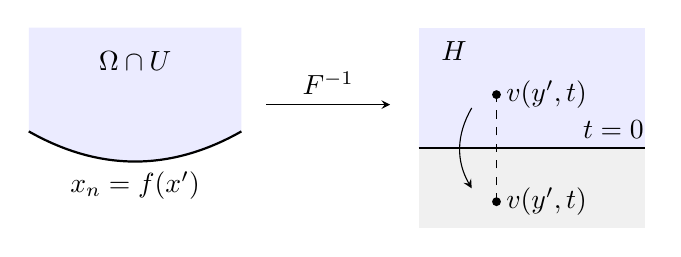
\begin{tikzpicture}[x=.9cm,y=.85cm,>=stealth]
	\fill[blue!8] (0,.25) .. controls (1,-.35) and (2,-.35) .. (3,.25) -- (3,1.8)--(0,1.8)--cycle;
	\draw[thick] (0,.25) .. controls (1,-.35) and (2,-.35) .. (3,.25);
	\node at (1.5,1.3) {\(\Omega\cap U\)};
	\node[below] at (1.5,-.2) {\(x_n=f(x')\)};
	\draw[->] (3.35,.65)--(5.1,.65) node[midway,above] {\(F^{-1}\)};
	\fill[blue!8] (5.5,0) rectangle (8.7,1.8);
	\fill[gray!12] (5.5,-1.2) rectangle (8.7,0);
	\draw[thick] (5.5,0)--(8.7,0);
	\node[above] at (8.25,0) {\(t=0\)};
	\node at (6,1.45) {\(H\)};
	\draw[dashed] (6.6,-.8)--(6.6,.8);
	\fill (6.6,.8) circle (1.6pt) node[right] {\(v(y',t)\)};
	\fill (6.6,-.8) circle (1.6pt) node[right] {\(v(y',t)\)};
	\draw[->] (6.25,.6) to[bend right=30] (6.25,-.6);
\end{tikzpicture}

	\caption[边界展平与反射延拓]{边界展平与反射延拓。左边的图形边界经 \(F^{-1}\) 变为右边的 \(t=0\)；下半空间的值由上半空间对称点的值给定。局部截断使图的侧边不产生新的跳跃。}
	\label{g3:fig:boundary-extension}
\end{figure}

这个定理使有界 \(C^1\) 域满足\cref{g3:def:sobolev-extension-domain}的延拓条件。由\cref{g3:thm:euclidean-sobolev,g3:prop:critical-sobolev,g3:thm:local-morrey}，先对 \(Eu\) 使用全空间估计再限制回来，得到区域上的连续嵌入：当 \(1\le p<n\) 时，\(W^{1,p}(\Omega)\) 嵌入 \(L^{np/(n-p)}(\Omega)\)；当 \(p=n\ge2\) 时，嵌入每个有限 \(L^q\)；当 \(p>n\) 时，有指数 \(1-n/p\) 的连续代表直到边界。\Cref{g3:thm:rellich-domain}同时给出这些嵌入在严格次临界范围内的紧性。一般函数的估计右侧采用完整 \(W^{1,p}\) 范数，因而包含 \(\|u\|_{L^p}\) 项。

\subsection{迹映射的连续性}
\label{g3:subsec:1106:02}
一个 \(L^p(\Omega)\) 等价类可以任意改变边界上的取值，所以不能直接把代表限制到 \(\partial\Omega\)。所需边界值应由内部逼近确定，并且不同逼近必须给出同一结果。一维估计提供了这种唯一性。

\begin{theorem}\label{g3:thm:sobolev-trace}
	设 \(\Omega\subset\mathbb R^n\) 为有界 \(C^1\) 域，\(1\le p<\infty\)，边界测度记为 \(\mathrm dS\)；\(n=1\) 时取端点计数测度。存在唯一有界线性\term[ji yingshe]{迹映射}[trace operator]
	\[
		\operatorname{Tr}:W^{1,p}(\Omega)\longrightarrow L^p(\partial\Omega,\mathrm dS),
	\]
	它在环境光滑函数上等于通常的边界限制。存在 \(h_0>0\) 及 \(C\)，使对 \(0<h<h_0\) 有
	\begin{equation}\label{g3:eq:trace-layer-bound}
		\|\operatorname{Tr}u\|_{L^p(\partial\Omega)}^p
		\le C\left(h^{-1}\|u\|_{L^p(\Omega)}^p
		+h^{p-1}\|\mathrm Du\|_{L^p(\Omega)}^p\right).
	\end{equation}
	若 \(1<p<\infty\)，则对每个 \(\varepsilon>0\)，存在 \(C_\varepsilon\) 使
	\begin{equation}\label{g3:eq:trace-epsilon-bound}
		\|\operatorname{Tr}u\|_{L^p(\partial\Omega)}^p
		\le\varepsilon\|\mathrm Du\|_{L^p(\Omega)}^p
		+C_\varepsilon\|u\|_{L^p(\Omega)}^p.
	\end{equation}
	若 \(u\in W^{1,p}(\Omega)\cap C(\overline\Omega)\)，其迹等于连续代表在边界的值，几乎处处成立。
\end{theorem}
\begin{proof}
	先对平半柱中的光滑函数 \(v(y',t)\) 使用微积分基本公式。对 \(0<t<h\)，有
	\[
		|v(y',0)|^p
		\le2^{p-1}|v(y',t)|^p
		+2^{p-1}t^{p-1}\int_0^t|\partial_t v(y',s)|^p\,\mathrm ds.
	\]
	这里 \(p=1\) 直接用积分三角不等式，其余情形用 Hölder 不等式。对 \(t\in(0,h)\) 取平均，再对 \(y'\) 积分，得到
	\[
		\int|v(y',0)|^p\,\mathrm dy'
		\le2^{p-1}\left(h^{-1}\int_0^h\!\int|v|^p\,\mathrm dy'\mathrm dt
		+h^{p-1}\int_0^h\!\int|\partial_t v|^p\,\mathrm dy'\mathrm dt\right).
	\]
	在每个边界图中令 \(v=(\chi_a u)\circ F\)。表面积元是 \(\sqrt{1+|\mathrm Df|^2}\,\mathrm dy'\)，它与 \(\mathrm dy'\) 一致可比。换元和乘法估计把右侧变成 \(u\) 与 \(\mathrm Du\) 的积分；由 \(\mathrm D\chi_a\) 产生的 \(h^{p-1}\|u\|_p^p\) 项在 \(h<h_0\le1\) 时并入 \(h^{-1}\|u\|_p^p\)。有限求和即得式\eqref{g3:eq:trace-layer-bound}。

	固定一个允许的 \(h\)，便得光滑函数的有界迹估计。由\cref{g3:thm:sobolev-extension-c1}的稠密性，若 \(u_j\to u\) 于 \(W^{1,p}\)，则边界限制 \(u_j|_{\partial\Omega}\) 是 \(L^p(\partial\Omega)\) 中的 Cauchy 列。定义其极限为 \(\operatorname{Tr}u\)。同一估计应用于两个逼近序列之差，证明定义无关；它也证明线性、有界性及唯一性，并使薄层估计延续到全部 \(u\)。当 \(p>1\) 时，选 \(h\) 使 \(Ch^{p-1}\le\varepsilon\)，即得式\eqref{g3:eq:trace-epsilon-bound}。

	若 \(u\) 在闭包连续，前一定理中的反射、截断和有限求和给出一个连续紧支延拓。它的卷积同时在闭包上一致收敛到 \(u\)，又在 \(W^{1,p}\) 中收敛。因此其边界限制的 \(L^p\) 极限就是 \(u|_{\partial\Omega}\)，证明最后一项。
\end{proof}
\symidx{\(\operatorname{Tr}u\)：Sobolev 函数或截面的边界迹}

薄层估计还显示了尺度。对一个固定的 \(C^1\) 域 \(\Omega_1\) 及 \(\Omega_R=R\Omega_1\)，换元 \(x=Ry\) 给出
\[
	\|\operatorname{Tr}u\|_{L^p(\partial\Omega_R)}^p
	\le C\left(R^{-1}\|u\|_{L^p(\Omega_R)}^p
	+R^{p-1}\|\mathrm Du\|_{L^p(\Omega_R)}^p\right).
\]
左侧在缩放中有 \(n-1\) 维的因子，两个右侧项恰有相同尺度。

\ProseParagraphBreak

\(p=1\) 时，式\eqref{g3:eq:trace-layer-bound}仍成立，但梯度前的系数不随 \(h\downarrow0\) 消失。例如在一个平边界片取非零光滑紧支 \(\psi(y')\)，再取 \(\eta(0)=1\)、支集位于 \([0,1)\) 的光滑函数，令 \(v_\delta(y',t)=\psi(y')\eta(t/\delta)\)。它的内部 \(L^1\) 范数趋零，\(\|\mathrm Dv_\delta\|_{L^1}\) 保持有界，而边界迹恒为 \(\psi\)。选足够小的固定 \(\varepsilon\) 就能看出，一般不能把式\eqref{g3:eq:trace-epsilon-bound}中的任意小系数结论扩展到 \(p=1\)。

\begin{proposition}\label{g3:prop:weak-boundary-integration}
	设 \(\Omega\subset\mathbb R^n\) 为有界 \(C^1\) 域，\(1\le p<\infty\)，\(u\in W^{1,p}(\Omega)\)，\(\phi\) 在 \(\overline\Omega\) 的邻域中光滑。若 \(\nu\) 为外单位法向，则
	\begin{equation}\label{g3:eq:weak-boundary-integration}
		\int_\Omega u\,\partial_i\phi\,\mathrm dx
		=-\int_\Omega(\partial_i u)\phi\,\mathrm dx
		+\int_{\partial\Omega}(\operatorname{Tr}u)\phi\nu_i\,\mathrm dS.
	\end{equation}
\end{proposition}
\begin{proof}
	先取光滑 \(u\)。在图形区域 \(x_n>f(x')\) 内，沿 \(x_n\) 积分给出下端点项；切向积分时，对变动下限 \(f(x')\) 求导，给出 \(\partial_i f\) 的因子。这恰是
	\[
		\nu\,\mathrm dS=(\mathrm Df,-1)\,\mathrm dx'
	\]
	的各分量。用单位分解求和，内部片无边界项，单位分解的导数因其总和为一而相消，得到光滑函数的公式。最后用贴边光滑函数在 \(W^{1,p}\) 中逼近 \(u\)。区域和边界测度都有限，内部两项按 \(L^p\) 收敛，边界项按迹的连续性收敛，故公式成立。
\end{proof}

\subsection{零边界 Sobolev 空间}
\label{g3:subsec:1106:03}
\(W_0^{1,p}(\Omega)\) 按定义是 \(C_c^\infty(\Omega)\) 的 \(W^{1,p}\) 闭包。它首先描述可逼近性。下面证明，在规则边界上，这个闭包恰好实现零边界值；零延拓是否产生额外边界导数是两种描述之间的联系。

\begin{theorem}\label{g3:thm:zero-trace-characterization}
	设 \(\Omega\subset\mathbb R^n\) 为有界 \(C^1\) 域，\(1\le p<\infty\)，\(u\in W^{1,p}(\Omega)\)。记 \(\widetilde u\) 为 \(u\) 在 \(\mathbb R^n\setminus\Omega\) 上补零的函数。则以下条件等价：
	\begin{equivalences}
		\item \(u\in W_0^{1,p}(\Omega)\)；
		\item \(\operatorname{Tr}u=0\)；
		\item \(\widetilde u\in W^{1,p}(\mathbb R^n)\)。
	\end{equivalences}
	此时 \(\partial_i\widetilde u=\widetilde{\partial_i u}\)，几乎处处成立。
\end{theorem}
\begin{proof}
	若 \(u\in W_0^{1,p}\)，用紧支于 \(\Omega\) 的光滑函数逼近。它们的迹都是零，故由连续性得到第二项；它们的零延拓及其导数在全空间同样是 Cauchy 列，故也得到第三项及所列导数公式。

	若 \(\operatorname{Tr}u=0\)，对任意 \(\phi\in C_c^\infty(\mathbb R^n)\)，式\eqref{g3:eq:weak-boundary-integration}成为
	\[
		\int_{\mathbb R^n}\widetilde u\,\partial_i\phi\,\mathrm dx
		=-\int_{\mathbb R^n}\widetilde{\partial_i u}\,\phi\,\mathrm dx.
	\]
	右侧由一个 \(L^p\) 函数给出，所以零延拓属于 \(W^{1,p}\)，并具有指定弱导数。

	现在从第三项构造内部紧支逼近。这一步既适用于 \(p>1\)，也适用于 \(p=1\)。用前述有限单位分解将 \(u\) 分成内部项与边界项。内部项离边界有正距离，直接卷积即可。对边界项，将其零延拓通过展平坐标拉回，得到一个紧支 \(w\in W^{1,p}(\mathbb R^n)\)，且 \(w=0\) 于 \(t<0\)。令
	\[
		w_\delta(y',t)=w(y',t-\delta),\qquad \delta>0.
	\]
	这将支集向区域内部移动，因而 \(w_\delta=0\) 于 \(t<\delta\)。由 \(L^p\) 平移连续性，函数及其全部一阶弱导数都收敛，所以 \(w_\delta\to w\) 于 \(W^{1,p}\)。再取卷积半径 \(\varepsilon_\delta<\delta/2\)，使卷积误差趋零。所得光滑函数的支集仍在 \(t>\delta/2\)，并可使其始终留在原来较大的坐标图内。

	将这些函数送回原坐标，得到离 \(\partial\Omega\) 有正距离的紧支 \(C^1\) 函数。若边界图只有 \(C^1\)，再对每个这样的函数在原 Euclid 坐标中作一次足够小半径的卷积，便得到 \(C_c^\infty(\Omega)\) 函数，且误差可任意小。换元估计保证此前的收敛仍为 \(W^{1,p}\) 收敛。有限个局部项相加，就得到逼近 \(u\) 的内部紧支光滑序列，证明第一项。
\end{proof}

例如区间上的常函数一属于 \(W^{1,p}(0,1)\)，但不属于 \(W_0^{1,p}(0,1)\)。它的零延拓是区间的示性函数，分布导数为 \(\delta_0-\delta_1\)，并非 \(L^p\) 函数。边界跳跃恰对应刚才分部积分中没有消失的边界项。

\ProseParagraphBreak

对非零给定边界数据，若已选定一个提升 \(g\in W^{1,p}(\Omega)\)，则所有满足 \(\operatorname{Tr}u=\operatorname{Tr}g\) 的函数恰为
\[
	g+W_0^{1,p}(\Omega).
\]
这是迹的线性与核的刻画直接给出的仿射空间。以后构造弱解时，减去 \(g\) 就把边界条件化为零边界条件。

\subsection{边界正则性的作用}
\label{g3:subsec:1106:04}
前面的常数来自有限个图的大小、展平映射及逆映射的导数、表面积元与单位分解。对一族区域，如果这些量一致受控，构造就给出一致的延拓与迹估计。仅知道各个区域分别有光滑边界，并不能使这些常数自动一致。

\begin{proposition}\label{g3:prop:sobolev-boundary-bundles}
	设 \((M,g)\) 为紧的光滑 \(n\) 维带边界黎曼流形，\(E\to M\) 为带光滑纤维度量及相容联络的有限秩实或复向量丛，\(1\le p<\infty\)。则存在有界线性映射
	\[
		\operatorname{Tr}:W^{1,p}(M;E)\longrightarrow
		L^p(\partial M;E|_{\partial M}),
	\]
	它延拓光滑截面的边界限制，且
	\[
		\ker\operatorname{Tr}=W_0^{1,p}(M;E),
	\]
	右侧为内部紧支光滑截面的闭包。式\eqref{g3:eq:trace-layer-bound}和 \(p>1\) 时的式\eqref{g3:eq:trace-epsilon-bound}也成立，将 \(\mathrm D\) 换为 \(\nabla\)、体积及表面积换为诱导的密度即可。相应的一阶嵌入范围为：
	\begin{enumerate}
		\item 当 \(1\le p<n\) 时，连续嵌入 \(L^q(M;E)\)，\(1\le q\le np/(n-p)\)；严格小于该上端点时嵌入为紧。
		\item 当 \(p=n\ge2\) 时，对每个 \(1\le q<\infty\)，到 \(L^q(M;E)\) 的嵌入为紧，因而连续。
		\item 当 \(p>n\) 时，连续嵌入 \(C^{0,\alpha}(M;E)\)，\(\alpha=1-n/p\)；到 \(C^{0,\beta}(M;E)\) 的嵌入在 \(0\le\beta<\alpha\) 时为紧，这里 \(\beta=0\) 表示一致范数。
		\item 当 \(n=p=1\) 时，连续嵌入 \(C^0(M;E)\)，并紧嵌入每个有限 \(L^q(M;E)\)。
	\end{enumerate}
	Hölder 范数按有限坐标图与丛标架定义。
\end{proposition}
\begin{proof}
	取有限个内部图及边界半空间图，并在各图内选择光滑丛标架。将截面乘以单位分解后逐分量反射、卷积，得到直到边界都光滑的逼近截面。局部范数与 \(\sum(|u^a|^p+|\mathrm Du^a|^p)\) 的积分等价：体积密度和纤维度量有正的上下界，协变导数与普通导数相差有界联络系数乘以截面的零阶项。

	各分量的边界迹因而满足一致的有限图估计。在两组标架的交集，分量由一个光滑可逆矩阵联系；在光滑截面上，取边界值与该矩阵的限制相容。再用逼近与乘法连续性取极限，这个相容关系保留，所以局部迹粘成 \(E|_{\partial M}\) 的截面，与标架及单位分解无关。标量证明中的分部积分、零延拓和向内平移逐分量进行，证明核正是内部紧支光滑截面的闭包。

	对每个局部项用半空间延拓，再使用欧氏 Sobolev 与 Rellich 结论，便得到相应的连续嵌入与紧嵌入；紧性只需对有限个图依次取子列。范数等价负责把分量收敛还原成截面收敛。迹的薄层估计也逐图求和；联络及截断引入的零阶项并入已有零阶项，便得到所述两种估计。
\end{proof}

\begin{proposition}\label{g3:prop:higher-order-boundary-extension}
	设 \(k\ge1\) 为整数，\(\Omega\subset\mathbb R^n\) 是有界 \(C^k\) 域，\(1\le p<\infty\)。则存在有界线性延拓
	\[
		E_k:W^{k,p}(\Omega)\longrightarrow W^{k,p}(\mathbb R^n),
	\]
	其支集包含于一个固定紧集。该构造的常数由有限边界图及逆图直到 \(k\) 阶的导数和相应截断函数控制。
\end{proposition}
\begin{proof}
	半空间上的偶反射一般不能保留二阶弱导数，例如 \(v(t)=t\) 的偶反射为 \(|t|\)，其一阶导数在零处跳跃。为使直到 \(k-1\) 阶的法向导数匹配，选择 \(c_1,\ldots,c_k\) 满足
	\[
		\sum_{j=1}^k c_j(-j)^\ell=1,
		\qquad 0\le\ell\le k-1.
	\]
	这些系数存在且唯一：系数矩阵可逆，因为次数不超过 \(k-1\) 的多项式若在 \(-1,\ldots,-k\) 都为零，就恒为零。对在闭半空间光滑的 \(v\)，在 \(t<0\) 定义
	\[
		(E_kv)(y',t)=\sum_{j=1}^k c_jv(y',-jt),
	\]
	在 \(t\ge0\) 保留原值。上述等式使所有总阶数小于 \(k\) 的导数在两侧相接。逐次分部积分时，直到第 \(k\) 次求导都没有边界跳跃项。每项的 \(\ell\) 次法向导数只多出 \((-j)^\ell\)，再以 \(s=-jt\) 换元，便得到 \(W^{k,p}\) 范数界。

	这里所用的闭半空间光滑稠密性也可在任意整数阶直接建立。先在远处截断，随后将 \(v(y',t)\) 替换为 \(v(y',t+\delta)\)。后者在 \(t>-\delta\) 已有定义；其各阶弱导数在 \(H\) 上趋于原导数，这是将这些 \(L^p(H)\) 导数各自补零后应用平移连续性的结果。再在半径小于 \(\delta/2\) 内卷积，得到闭半空间附近光滑的函数；对所有不超过 \(k\) 阶的导数同时选择足够小的卷积半径，就得到 \(W^{k,p}(H)\) 逼近。因此前述有界反射算子可连续延拓到全部 \(W^{k,p}(H)\)。

	对一般 \(C^k\) 域，使用与一阶情形相同的有限覆盖、单位分解及展平。反复使用链式法则，\(C^k\) 图及逆图的有界导数控制全部不超过 \(k\) 阶的范数。将半空间延拓限制在足够薄的较大图内、乘截断后送回并求和，就得到所需算子与固定紧支集。
\end{proof}

这个证明说明了所选展平构造为何要求相应阶数的导数控制。\(C^1\) 边界也不是一阶延拓存在的必要条件：矩形的角点不满足 \(C^1\) 图形条件，但逐个坐标反射、再乘固定截断函数，仍给出一阶有界延拓。判断边界正则性时，要检查实际能否作有界的局部变换与拼接。

\begin{example}\label{g3:exm:slit-domain-traces}
	考虑去掉一条半径的单位圆盘
	\[
		\Omega=\{(r\cos\theta,r\sin\theta):0<r<1,\ 0<\theta<2\pi\}.
	\]
	取 \(\chi\in C_c^\infty((1/4,3/4))\)，且在一个较小区间上等于一，定义 \(u(r,\theta)=\chi(r)\theta\)。函数及其一阶导数在 \(\Omega\) 上有界，所以 \(u\in W^{1,p}(\Omega)\) 对每个有限 \(p\) 成立。裂缝的上侧边界值为零，下侧为 \(2\pi\chi(r)\)，两侧都来自各自半邻域中的光滑限制。

	不存在把这个 \(u\) 延拓到整个圆盘的 \(W^{1,p}\) 函数。事实上，对裂缝中 \(\chi=1\) 的一段，几乎每条横穿裂缝的竖直线在两侧都有相差 \(2\pi\) 的极限。若延拓属于 \(W^{1,p}\)，绝对连续切片判据要求同一条线上的代表跨过裂缝连续，矛盾。裂缝作为平面中的点集只有一份，但域内逼近有两侧；在这种区域上，边界值必须保留所从属的一侧。
\end{example}
% 纲要条目排为编号小节标题，并进入目录与书签；说明段仍保留于纲要注释中。


\begin{chaptersummary}
弱导数由分部积分确定，局部平滑与坐标变换保证这一概念能够用于流形及向量丛。整数阶 Sobolev 范数把截面与各阶弱协变导数放进一组 \(L^p\) 空间，闭图关系给出完备性；在 \(1<p<\infty\) 时，积分对偶和反射性给出有界序列的弱收敛子列。光滑稠密性、截断与链式法则使这些空间能够承接微分方程中的测试和非线性运算。

\ProseParagraphBreak

Sobolev 嵌入把导数可积性换成更高的函数可积性，Morrey 估计进一步产生连续代表。临界指数与高阶端点须按维数和导数阶数判断。Poincaré 不等式通过边界条件、均值或平行截面投影去掉导数的核；其常数记录着尺度与连通区域之间的联系。Rellich 紧性则把平移控制和尾部控制化为有限近似，在严格低于临界指数处得到强收敛子列。

\ProseParagraphBreak

边界展平与反射提供延拓，法向的一维微积分给出连续迹。对有界 \(C^1\) 域，零迹恰好刻画内部紧支光滑函数的 \(W^{1,p}\) 闭包，也恰好保证补零后仍有全局一阶弱导数；高阶延拓还要匹配更多阶的边界导数。下一章将在这些空间上建立弱椭圆方程，先由能量估计获得解，再用局部与边界正则性恢复更强的微分性质。
\end{chaptersummary}

\BookExercises

\begin{exercise}\label{g3:ex:circle-sawtooth-weak}
	在周长为 \(L>0\) 的圆周 \(S^1_L=\mathbb R/L\mathbb Z\) 上，用 \([0,L)\) 的代表定义 \(u([x])=x\)。以周期光滑测试函数定义分布导数，求 \(\partial_xu\)，并判断 \(u\) 是否属于 \(W^{1,p}(S^1_L)\)，\(1\le p\le\infty\)。
\end{exercise}
\begin{solution}
	对周期光滑函数 \(\varphi\)，分部积分给出
	\[
		-\int_0^L x\varphi'(x)\,\mathrm dx
		=\int_0^L\varphi(x)\,\mathrm dx-L\varphi(0).
	\]
	因此 \(\partial_xu=1-L\delta_{[0]}\)。该函数有界，属于每个 \(L^p\)，但其导数包含点质量。由\cref{g3:exm:point-distribution}，点质量不能由局部可积函数表示，故它不属于任何上述 \(W^{1,p}\)。在开区间 \((0,L)\) 中只看到导数一，圆周的端点识别却引入了一个大小为 \(-L\) 的跳跃。
\end{solution}

\begin{exercise}\label{g3:ex:weighted-interval-weak-laplacian}
	设 \(a\in C^\infty([0,1])\) 且 \(a>0\)，在区间上取度量 \(g=a(x)^2\mathrm dx^2\)。写出标量 \(H^1\) 范数与弱 Laplace 算子。再设 \(u\in H^1(0,1)\)、\(f\in L^1_{\mathrm{loc}}(0,1)\)，以 \(y=\int_0^x a(t)\,\mathrm dt\) 换坐标，证明这一范数及弱方程 \(\Delta_gu=f\) 分别变为长度为 \(\ell=\int_0^1a\) 的普通区间上的标准 \(H^1\) 范数及 \(-\partial_y^2\widetilde u=\widetilde f\)。
\end{exercise}
\begin{solution}
	体积密度为 \(a\,\mathrm dx\)，而 \(|\mathrm du|_g^2=a^{-2}|u'|^2\)，所以
	\[
		\|u\|_{H^1(g)}^2=\int_0^1\left(a|u|^2+a^{-1}|u'|^2\right)\,\mathrm dx.
	\]
	弱方程表示对每个内部紧支光滑 \(\varphi\) 有
	\[
		\int_0^1a^{-1}u'\varphi'\,\mathrm dx=\int_0^1fa\varphi\,\mathrm dx.
	\]
	因此在分布意义下 \(\Delta_gu=-a^{-1}\partial_x(a^{-1}u')\)。换元满足 \(\mathrm dy=a\,\mathrm dx\)、\(u'=a\partial_y\widetilde u\)，两个积分变成
	\[
		\int_0^\ell\left(|\widetilde u|^2+|\partial_y\widetilde u|^2\right)\,\mathrm dy,
		\qquad
		\int_0^\ell(\partial_y\widetilde u)(\partial_y\widetilde\varphi)\,\mathrm dy
		=\int_0^\ell\widetilde f\widetilde\varphi\,\mathrm dy.
	\]
	\(a\) 有正下界，换元及逆换元的一阶导数有界，故\cref{g3:prop:weak-coordinate-change}保证这些计算也适用于弱导数。最后的恒等式正是所述非负 Laplace 约定下的方程。
\end{solution}

\begin{exercise}\label{g3:ex:noncompact-connection-sobolev}
	在 \(\mathbb R\times\mathbb C\) 上取标准底度量和纤维 Hermitian 度量，比较两个相容联络
	\[
		\nabla=\mathrm d,\qquad\nabla'=\mathrm d+\mathrm i x\,\mathrm dx.
	\]
	设 \(1\le p<\infty\)，令 \(a=1/p+1/2\)、\(s(x)=(1+x^2)^{-a/2}\)。证明 \(s\in W^{1,p}_\nabla\)，但 \(s\notin W^{1,p}_{\nabla'}\)。解释这为何不与紧流形上的联络无关性矛盾。
\end{exercise}
\begin{solution}
	联络一形式 \(\mathrm ix\,\mathrm dx\) 是反 Hermitian 的，故 \(\nabla'\) 也保持标准纤维度量。无穷远处 \(|s|\) 与 \(|x|^{-a}\) 可比，\(|s'|\) 与 \(|x|^{-a-1}\) 可比；由于 \(ap=1+p/2>1\)，两者的 \(p\) 次幂都可积。因此 \(s\in W^{1,p}_\nabla\)。

	由于 \(s,s'\) 为实值，
	\[
		|\nabla's|^2=|s'+\mathrm ixs|^2=|s'|^2+x^2s^2.
	\]
	\(|xs|^p\) 在无穷远处与 \(|x|^{p(1-a)}\) 可比，其可积性要求 \((a-1)p>1\)；这里 \((a-1)p=1-p/2<1\)，所以不可积。两个联络之差的系数 \(x\) 无界，紧流形证明所用的统一系数界不成立。它们在每个固定紧区间上仍定义等价范数。
\end{solution}

\begin{exercise}\label{g3:ex:weak-strong-oscillation}
	在 \(S^1_{2\pi}\) 上令 \(u_j(x)=j^{-1}\sin(jx)\)，\(1<p<\infty\)。证明 \(u_j\to0\) 于每个有限 \(L^q\) 及一致范数，\(u_j\rightharpoonup0\) 于 \(W^{1,p}\)，但它没有 \(W^{1,p}\) 强收敛子列。
\end{exercise}
\begin{solution}
	由 \(\|u_j\|_\infty\le j^{-1}\)，得到全部所述零阶强收敛。一阶导数为 \(u_j'=\cos(jx)\)，其 \(L^p\) 范数恒等于 \(\|\cos x\|_{L^p(0,2\pi)}>0\)。若某子列在 \(W^{1,p}\) 中强收敛，零阶极限只能为零，导数范数也应趋零，矛盾。

	对周期光滑测试函数 \(\psi\)，分部积分给出
	\[
		\left|\int_0^{2\pi}\psi(x)\cos(jx)\,\mathrm dx\right|
		\le j^{-1}\|\psi'\|_{L^1}.
	\]
	光滑函数在 \(L^{p'}\) 中稠密，而 \(\cos(jx)\) 的 \(L^p\) 范数一致有界，故这一配对趋零对所有 \(L^{p'}\) 测试函数成立。因此 \((u_j,u_j')\rightharpoonup(0,0)\) 于 \(L^p\times L^p\)。\(W^{1,p}\) 是这个乘积空间的闭子空间，每个有界线性泛函都可按\cref{g3:lem:bounded-functional-extension}延拓，故这正给出 \(W^{1,p}\) 中的弱收敛。高频振荡可以保留导数范数，同时使每个固定测试配对趋零。
\end{solution}

\begin{exercise}\label{g3:ex:bundle-modulus-sharpness}
	在 \(S^1_{2\pi}\) 的平凡复线丛上取平坦联络。令 \(s_j(x)=e^{\mathrm ijx}\)。计算 \(\||s_j|\|_{W^{1,p}}\) 和 \(\|\nabla s_j\|_{L^p}\)，\(1\le p<\infty\)。说明模长估计不能反向控制截面的导数。再设在连通开集 \(U\subset\mathbb R^n\) 上有光滑表示 \(s=\rho e^{\mathrm i\theta}\)，其中 \(\rho>0\)、\(\theta\) 实值。证明模长不等式处处取等号，当且仅当 \(\theta\) 为常数。
\end{exercise}
\begin{solution}
	\(|s_j|=1\)，所以 \(\||s_j|\|_{W^{1,p}}=(2\pi)^{1/p}\)；而 \(|\nabla s_j|=j\)，故 \(\|\nabla s_j\|_p=j(2\pi)^{1/p}\)。模长不记录相位变化，因此不存在由模长的这个范数统一控制截面导数的反向估计。

	对第二问，直接计算得到
	\[
		\mathrm ds=e^{\mathrm i\theta}(\mathrm d\rho+\mathrm i\rho\,\mathrm d\theta),
		\qquad |\mathrm ds|^2=|\mathrm d\rho|^2+\rho^2|\mathrm d\theta|^2.
	\]
	由于 \(\rho>0\)，模长不等式处处取等号等价于 \(\mathrm d\theta=0\)。连通开集中的两点可以用有限条线段连接，沿每条线段应用微积分基本定理，便知这一条件等价于 \(\theta\) 为常数。
\end{solution}

\begin{exercise}\label{g3:ex:radial-sobolev-threshold}
	设 \(n\ge2\)、\(1\le p<n\)，\(\eta\in C_c^\infty(B_1(0))\) 在 \(B_{1/2}(0)\) 上等于一。对 \(a>0\)，令 \(u_a(x)=\eta(x)|x|^{-a}\)。求 \(u_a\in W^{1,p}(B_1)\) 的充要条件，以及 \(u_a\in L^q(B_1)\)（\(1\le q<\infty\)）的条件。由此说明在固定球中，\(W^{1,p}\) 嵌入的上限指数 \(p^*=np/(n-p)\) 不能提高。
\end{exercise}
\begin{solution}
	在零点以外，\(|\mathrm Du_a|=a|x|^{-a-1}\) 当 \(|x|<1/2\)。极坐标积分说明
	\[
		\int_0^{1/2}r^{n-1-aq}\,\mathrm dr<\infty
		\quad\Longleftrightarrow\quad aq<n,
	\]
	而梯度的 \(p\) 次幂可积当且仅当 \((a+1)p<n\)。等号时积分为 \(\int\mathrm dr/r\)，仍发散。

	若 \((a+1)p<n\)，则 \(a<n-1\)。在穿孔球上分部积分，内边界项至多为常数乘 \(\varepsilon^{n-1-a}\)，故趋零；经典导数于是给出全球弱导数，且 \(u_a\in L^p\)。反过来，若 \(u_a\) 属于 \(W^{1,p}\)，在任何避开零点的开集上，其弱导数必须等于已算出的经典导数，因此 \((a+1)p<n\) 必要。这得到充要条件。

	给定 \(q>p^*\)，有 \(n/q<n/p-1\)，故可取
	\(n/q\le a<n/p-1\)。此时 \(u_a\in W^{1,p}\) 却不在 \(L^q\)。由于它支于球内部，前述局部卷积也表明它属于 \(W_0^{1,p}(B_1)\)，所以即使加入零边界条件也不能提高最大指数。所有 \(a>0\) 的函数都在零附近无界，亦给出 \(L^\infty\) 失败。
\end{solution}

\begin{exercise}\label{g3:ex:morrey-sharp-exponent}
	设 \(n<p<\infty\)，令 \(\alpha=1-n/p\)。取 \(\varphi\in C_c^\infty(B_1(0))\)，满足 \(\varphi(0)=1\)，并定义
	\[
		u_\varepsilon(x)=\varepsilon^\alpha\varphi(x/\varepsilon),
		\qquad 0<\varepsilon<1/3.
	\]
	证明 \(u_\varepsilon\) 在 \(W^{1,p}(B_1)\) 中有界，而且一致趋于零；但对任何 \(\alpha<\beta\le1\)，\([u_\varepsilon]_{C^{0,\beta}(B_1)}\to\infty\)。说明这对 Morrey 指数的意义。
\end{exercise}
\begin{solution}
	换元给出
	\[
		\|u_\varepsilon\|_p=\varepsilon^{\alpha+n/p}\|\varphi\|_p
		=\varepsilon\|\varphi\|_p,\qquad
		\|\mathrm Du_\varepsilon\|_p=\varepsilon^{\alpha-1+n/p}\|\mathrm D\varphi\|_p
		=\|\mathrm D\varphi\|_p.
	\]
	且 \(\|u_\varepsilon\|_\infty=\varepsilon^\alpha\|\varphi\|_\infty\to0\)。另一方面，在 \(0\) 与 \(2\varepsilon e_1\) 两点的函数值分别为 \(\varepsilon^\alpha\)、零，因而
	\[
		[u_\varepsilon]_{C^{0,\beta}(B_1)}\ge2^{-\beta}\varepsilon^{\alpha-\beta}\longrightarrow\infty.
	\]
	因此原 Sobolev 范数不能统一控制任何更大的 Hölder 指数。每个函数自身虽光滑，这列函数在不断缩小的区域中仍有比 \(\beta\) 次幂更强的振荡；一致收敛也不能给出高阶模连续性的统一界。
\end{solution}

\begin{exercise}\label{g3:ex:sobolev-multiplication-threshold}
	设 \((M^n,g)\) 为紧、光滑、无边界黎曼流形，\(n<p<\infty\)。用本章乘法代数的范数估计证明，对每个实值 \(u\in W^{1,p}(M)\)，指数级数在 \(W^{1,p}\) 中收敛，且
	\[
		e^u-1\in W^{1,p}(M),\qquad
		\|e^u-1\|_{W^{1,p}}\le\|u\|_{W^{1,p}}\exp\bigl(C\|u\|_{W^{1,p}}\bigr).
	\]
	证明其弱导数为 \(e^u\,\mathrm du\)。再在 \(n\ge2\)、\(1\le p<n\) 的情形，构造支于一个坐标球的 \(u\in W^{1,p}(M)\)，使 \(u^2\notin W^{1,p}(M)\)。
\end{exercise}
\begin{solution}
	令 \(C\ge1\) 为\cref{g3:cor:sobolev-multiplication-algebra}中 \(k=1\) 的常数，记 \(A=\|u\|_{W^{1,p}}\)。归纳得到 \(\|u^j\|_{W^{1,p}}\le C^{j-1}A^j\)，故
	\[
		\sum_{j=1}^\infty\left\|\frac{u^j}{j!}\right\|_{W^{1,p}}
		\le A\sum_{j=1}^\infty\frac{(CA)^{j-1}}{j!}\le A e^{CA}.
	\]
	由完备性，该级数在 \(W^{1,p}\) 中收敛。\cref{g3:thm:compact-bundle-sobolev}给出到 \(C^0\) 的连续嵌入，所以它也一致收敛；逐点普通指数级数将极限识别为 \(e^u-1\)。对部分和使用弱乘积公式，其导数为
	\[
		\left(\sum_{j=1}^N\frac{u^{j-1}}{(j-1)!}\right)\mathrm du.
	\]
	括号中的级数一致趋于 \(e^u\)，乘 \(L^p\) 的 \(\mathrm du\) 后在 \(L^p\) 中收敛，故弱导数正是所述公式。

	当 \(p<n\) 时，记 \(A=n/p-1>0\)，选择
	\[
		\frac A2<a<\min\left\{A,\frac n{2p}\right\}.
	\]
	右端严格大于左端，故可选到。取坐标球内的紧支截断，定义 \(u=\eta(x)|x|^{-a}\)，在球外补零。度量及体积密度在截断支集上与 Euclid 数据一致可比，\cref{g3:ex:radial-sobolev-threshold}的计算给出 \(u\in W^{1,p}(M)\)。同时 \(2ap<n\)，故 \(u^2\in L^p\)；但 \((2a+1)p>n\)，其在穿孔小球中的经典梯度不属于 \(L^p\)。若存在全局 \(L^p\) 弱导数，它在这个穿孔区域中必须与该梯度一致，产生矛盾。因此乘法闭性确实失败。
\end{solution}

\begin{exercise}\label{g3:ex:poincare-positive-measure-anchor}
	设 \((M,g)\) 为连通、紧且无边界的光滑黎曼流形，\(1\le p<\infty\)，其零均值 Poincaré 常数为 \(C_P\)。设可测集 \(A\subset M\) 满足 \(\operatorname{Vol}(A)\ge a>0\)。证明：若 \(u\in W^{1,p}(M)\) 且 \(u=0\) 几乎处处于 \(A\)，则
	\[
		\|u\|_{L^p(M)}\le C_P\left[1+\left(\frac{\operatorname{Vol}(M)}a\right)^{1/p}\right]\|\mathrm du\|_{L^p(M)}.
	\]
	再解释将“正测度集上为零”换成“某一点取值为零”时，在 \(n=\dim M\ge2\)、\(p\le n\) 的一般 Sobolev 类中为什么需要重新定义条件。
\end{exercise}
\begin{solution}
	令 \(c=u_M\)。在 \(A\) 上有 \(u-c=-c\)，故
	\[
		|c|a^{1/p}\le\|u-c\|_{L^p(A)}\le C_P\|\mathrm du\|_{L^p(M)}.
	\]
	由三角不等式，
	\[
		\|u\|_p\le\|u-c\|_p+|c|\operatorname{Vol}(M)^{1/p},
	\]
	代入前式即得所求常数。

	Sobolev 元素是几乎处处相等的函数类，改变一个点的取值不改变该元素，也不改变弱导数。若尚未通过连续代表或其他附加结构定义点值，“某一点为零”可由任意函数通过修改零测集实现，因而不能消除常数核。\(p>n\) 时 Morrey 连续代表提供了真正的点值，才可另行讨论以点为锚的估计。
\end{solution}

\begin{exercise}\label{g3:ex:product-poincare-optimal}
	设 \(M,N\) 为正维、连通、紧且无边界的光滑黎曼流形。令 \(C_M,C_N\) 分别为 \(L^2\) 零均值 Poincaré 不等式的最佳常数。证明乘积度量下的最佳常数满足
	\[
		C_{M\times N}=\max\{C_M,C_N\}.
	\]
	证明中不使用 Laplace 特征函数展开。
\end{exercise}
\begin{solution}
	对光滑函数 \(u(x,y)\)，令 \(v(y)=\operatorname{Vol}(M)^{-1}\int_Mu(x,y)\mu_M(x)\)，\(c=u_{M\times N}\)。对每个 \(y\)，\(u-v\) 在 \(M\) 上均值为零，所以 \(u-v\) 与仅依赖 \(y\) 的 \(v-c\) 在乘积 \(L^2\) 内积中正交。因此
	\[
		\|u-c\|_2^2=\|u-v\|_2^2+\|v-c\|_2^2.
	\]
	对第一项逐个 \(M\) 纤维应用不等式，得 \(\|u-v\|_2^2\le C_M^2\|\mathrm d_Mu\|_2^2\)。对第二项在 \(N\) 上应用不等式，并用积分平均的凸性，得
	\[
	\begin{aligned}
		\|v-c\|_{L^2(M\times N)}^2
		&\le C_N^2\operatorname{Vol}(M)\int_N|\mathrm d_Nv|^2\mu_N\\
		&\le C_N^2\|\mathrm d_Nu\|_{L^2(M\times N)}^2.
	\end{aligned}
	\]
	乘积度量使两种梯度平方相加，因而 \(C_{M\times N}\le\max\{C_M,C_N\}\)。光滑稠密性将此估计推广到 \(W^{1,2}\)。反过来，依次取只依赖 \(x\) 或只依赖 \(y\) 的非恒定函数，乘积体积因子在函数范数与梯度范数的比值中抵消，故最佳常数至少分别为 \(C_M,C_N\)。
\end{solution}

\begin{exercise}\label{g3:ex:quantitative-sobolev-finite-net}
	设 \(Q=(0,1)^n\)、\(1\le p<\infty\)，并令
	\[
		\mathcal F=\{u\in W^{1,p}(Q;\mathbb R):u_Q=0,\ \|\mathrm D u\|_{L^p(Q)}\le1\}.
	\]
	把 \(Q\) 分成 \(m^n\) 个边长 \(1/m\) 的小立方体，在每个小立方体上以平均值代替 \(u\)，所得算子记为 \(A_m\)。证明
	\[
		\|u-A_mu\|_{L^p(Q)}\le\frac{2^{n/p}\sqrt n}{m}.
	\]
	再证明存在只依赖 \(n,p\) 的常数 \(C\ge2\)，使 \(0<\varepsilon<1\) 时，\(\mathcal F\) 在 \(L^p(Q)\) 中有一个精度 \(\varepsilon\) 的有限近似集，其点数至多为
	\[
		\exp\!\left(C\varepsilon^{-n}\log\frac C\varepsilon\right).
	\]
	近似集的元素允许为分块常值函数。
\end{exercise}
\begin{solution}
	每个小立方体直径为 \(\sqrt n/m\)。由\cref{g3:prop:poincare-convex-mean}，将各块误差的 \(p\) 次方相加，立即得到第一式。对整个 \(Q\) 使用同一命题，还知 \(\|u\|_p\le C_0=2^{n/p}\sqrt n\)。

	对体积为 \(m^{-n}\) 的任一小块 \(Q_\nu\)，Hölder 不等式给出
	\[
		|u_{Q_\nu}|\le m^{n/p}\|u\|_{L^p(Q_\nu)}\le C_0m^{n/p}.
	\]
	取 \(m=\lceil2C_0/\varepsilon\rceil\)，使平均化误差至多为 \(\varepsilon/2\)。在区间 \([-C_0m^{n/p},C_0m^{n/p}]\) 上取间距不超过 \(\varepsilon\) 的等距刻度，把每个块平均值替换成最近刻度值。各点误差至多为 \(\varepsilon/2\)，而 \(|Q|=1\)，所以新增 \(L^p\) 误差也至多为 \(\varepsilon/2\)。

	每块可选刻度数至多为 \(2+2C_0m^{n/p}/\varepsilon\)，全部分块常值函数数目因而至多为
	\[
		\left(2+\frac{2C_0m^{n/p}}\varepsilon\right)^{m^n}.
	\]
	由于 \(m\le C_1/\varepsilon\)，对上式取对数并吸收只依赖 \(n,p\) 的常数，即得题设上界。这是一个明确的近似规模估计，未断言该数量级最优。
\end{solution}

\begin{exercise}\label{g3:ex:weak-and-strong-sobolev-limits}
	设 \((M^n,g)\) 为紧且无边界的光滑黎曼流形。
	\begin{enumerate}
		\item 设 \(1<p<\infty\)，\(u_j\) 是 \(W^{1,p}(M)\) 中的有界序列，且 \(u_j\rightharpoonup u\)。证明在\cref{g3:thm:compact-bundle-rellich}允许的每个有限 \(L^q\) 范数中，整个序列都强收敛到 \(u\)。
		\item 在区间 \((-1,1)\) 上构造 \(W^{1,1}\) 有界的光滑函数列，在每个有限 \(L^q\) 中强收敛到不属于 \(W^{1,1}\) 的函数。计算其导数的分布极限。
	\end{enumerate}
\end{exercise}
\begin{solution}
	1. 若某个允许的 \(L^q\) 范数中的强收敛不成立，存在 \(\varepsilon>0\) 和子列，使 \(\|u_j-u\|_q\ge\varepsilon\)。紧嵌入给出进一步子列在 \(L^q\) 中强收敛到某个 \(v\)。对任意光滑测试函数，弱 \(W^{1,p}\) 收敛使积分配对趋于 \(u\) 的配对，强 \(L^q\) 收敛使同一配对趋于 \(v\) 的配对。因此 \(u=v\) 几乎处处，与距离下界矛盾。紧性加上极限的唯一识别，消除了再次抽子列的需要。

	2. 取光滑非减函数 \(\eta:\mathbb R\to[0,1]\)，使 \(\eta(t)=0\) 当 \(t\le-1\)，\(\eta(t)=1\) 当 \(t\ge1\)。令 \(u_j(x)=\eta(jx)\)。有 \(\|u_j\|_1\le2\) 及
	\[
		\int_{-1}^1|u_j'(x)|\,\mathrm dx=1.
	\]
	它与阶跃函数 \(H=\mathbf1_{(0,1)}\) 只在长度 \(2/j\) 的区间内可能不同，且差值不超过一，故 \(\|u_j-H\|_q\le(2/j)^{1/q}\to0\)。对任意 \(\phi\in C_c^\infty(-1,1)\)，
	\[
		\int_{-1}^1u_j'\phi\,\mathrm dx=-\int_{-1}^1u_j\phi'\,\mathrm dx
		\longrightarrow-\int_0^1\phi'\,\mathrm dx=\phi(0).
	\]
	导数的分布极限为点质量 \(\delta_0\)，它不能由 \(L^1\) 函数表示：若能，取支集缩向零、值在零到一之间且在零点为一的测试函数，积分的绝对连续性会使配对趋零，与恒等于一矛盾。因此 \(H\notin W^{1,1}(-1,1)\)。强 \(L^q\) 紧性并不保证 \(p=1\) 时极限仍有 \(L^1\) 弱导数。
\end{solution}

\begin{exercise}\label{g3:ex:sobolev-tightness-moment}
	设 \(n\ge1\)、\(1\le p<\infty\)、\(a>0\)。证明函数族
	\[
		\mathcal F=\left\{u\in W^{1,p}(\mathbb R^n):
		\|u\|_{W^{1,p}}\le1,\quad
		\int_{\mathbb R^n}|x|^a|u(x)|^p\,\mathrm dx\le1\right\}
	\]
	在 \(L^p(\mathbb R^n)\) 中相对紧。若 \(p<n\)，进一步证明它在每个 \(L^q(\mathbb R^n)\)、\(p\le q<np/(n-p)\) 中相对紧。
\end{exercise}
\begin{solution}
	当 \(R>0\) 时，
	\[
		\int_{|x|>R}|u|^p\,\mathrm dx\le R^{-a}\int_{|x|>R}|x|^a|u|^p\,\mathrm dx\le R^{-a}.
	\]
	因此有统一的尾部控制。\cref{g3:lem:sobolev-translation-bound}又给出 \(\|\tau_hu-u\|_p\le|h|\)，而范数有界是题设。\Cref{g3:thm:lp-translation-compactness}遂给出 \(L^p\) 相对紧性。

	当 \(p<n\) 时，全空间 Sobolev 不等式给出统一的 \(L^{p^*}\) 界。对任意 \(p<q<p^*\)，用式\eqref{g3:eq:rellich-interpolation}将已取得的 \(L^p\) 强收敛与 \(L^{p^*}\) 有界性插值，即得 \(L^q\) 强收敛子列。矩条件通过排除质量远移，使非紧底空间仍能产生全局紧性。
\end{solution}

\begin{exercise}\label{g3:ex:circle-connection-poincare}
	在周长为 \(L>0\) 的圆周上取平凡复线丛，标准 Hermitian 度量和联络
	\[
		\nabla_a u=(u'+\mathrm iau)\,\mathrm dt,\qquad a\in\mathbb R.
	\]
	求其平行截面空间。当 \(aL\notin2\pi\mathbb Z\) 时，不用 Fourier 展开，证明
	\[
		\|u\|_{L^2}\le L\left(1+\frac1{|e^{\mathrm iaL}-1|}\right)\|\nabla_a u\|_{L^2}
	\]
	对所有 \(u\in W^{1,2}(S^1_L;\mathbb C)\) 成立，并证明当非零 \(a\to0\) 时，任何这样的无核估计常数必趋于无穷。
\end{exercise}
\begin{solution}
	平行方程的解为 \(u(t)=ce^{-\mathrm iat}\)。周期条件要求 \((e^{-\mathrm iaL}-1)c=0\)，故 \(aL\in2\pi\mathbb Z\) 时平行空间为一维，否则为零。

	先设 \(u\) 光滑，记 \(f=u'+\mathrm iau\)。乘以积分因子并从零积分，得
	\[
		u(t)=e^{-\mathrm iat}\left(c+\int_0^te^{\mathrm ias}f(s)\,\mathrm ds\right).
	\]
	周期条件给出
	\[
		(e^{\mathrm iaL}-1)c=\int_0^Le^{\mathrm ias}f(s)\,\mathrm ds,
		\qquad |c|\le\frac{\sqrt L}{|e^{\mathrm iaL}-1|}\|f\|_2.
	\]
	另有 \(\left|\int_0^te^{\mathrm ias}f(s)\,\mathrm ds\right|\le\sqrt L\|f\|_2\)。把逐点估计在长度 \(L\) 的圆周上取 \(L^2\) 范数，即得题设不等式；光滑稠密性将其推广到 \(W^{1,2}\)。

	最后取 \(u\equiv1\)。其函数范数为 \(\sqrt L\)，协变导数范数为 \(|a|\sqrt L\)，所以任何无核估计常数至少为 \(1/|a|\)。当 \(a\to0\) 时，平行核即将出现，常数相应发散；即使底空间与纤维度量都固定，联络的变化也会影响能量估计。
\end{solution}

\begin{exercise}\label{g3:ex:zero-trace-second-order}
	设 \(1\le p<\infty\)，在 \((0,1)\) 上令 \(u(t)=t(1-t)\)。证明
	\[
		u\in W^{2,p}(0,1)\cap W_0^{1,p}(0,1),
		\qquad u\notin W_0^{2,p}(0,1).
	\]
	计算 \(u\) 的零延拓在 \(\mathbb R\) 上的二阶分布导数，并说明为什么仅令函数的迹为零不能保证二阶零延拓属于 \(W^{2,p}\)。
\end{exercise}
\begin{solution}
	\(u\) 是多项式，各阶所需导数均有界，故属于 \(W^{2,p}\)。它在两端点为零，由\cref{g3:thm:zero-trace-characterization}可知 \(u\in W_0^{1,p}\)。如果还有 \(u\in W_0^{2,p}\)，则存在 \(\phi_j\in C_c^\infty(0,1)\) 趋于 \(u\) 于 \(W^{2,p}\)，从而 \(\phi_j'\to u'\) 于 \(W^{1,p}\)。迹的连续性迫使 \(u'\) 在两端的迹都是零；但 \(u'(0)=1\)、\(u'(1)=-1\)，矛盾。

	记零延拓为 \(\widetilde u\)。一次求导没有边界项，因为 \(u(0)=u(1)=0\)，故
	\[
		\widetilde u'=(1-2t)\mathbf1_{(0,1)}.
	\]
	再次对测试函数分部积分，得到
	\[
		\widetilde u''=-2\mathbf1_{(0,1)}+\delta_0+\delta_1.
	\]
	两个点质量项分别来自一阶导数在端点的跳跃。它们不是 \(L^p\) 函数，所以 \(\widetilde u\notin W^{2,p}(\mathbb R)\)。因此 \(W^{2,p}\cap W_0^{1,p}\) 与 \(W_0^{2,p}\) 表达不同的边界条件。
\end{solution}

\begin{exercise}\label{g3:ex:boundary-energy-lower-bound}
	设 \(\Omega\subset\mathbb R^n\) 为有界 \(C^1\) 域，\(\beta\in L^\infty(\partial\Omega;\mathbb R)\)。对实值 \(u\in W^{1,2}(\Omega)\) 定义
	\[
		Q(u)=\int_\Omega|\mathrm Du|^2\,\mathrm dx
		+\int_{\partial\Omega}\beta|\operatorname{Tr}u|^2\,\mathrm dS.
	\]
	证明存在 \(\lambda>0\)，使对所有 \(u\in W^{1,2}(\Omega)\)，
	\[
		Q(u)+\lambda\|u\|_{L^2(\Omega)}^2
		\ge\frac12\|\mathrm Du\|_{L^2(\Omega)}^2
		+\|u\|_{L^2(\Omega)}^2.
	\]
	这里 \(\beta\) 可以取负值。另证明相应双线性型
	\(\int_\Omega\langle\mathrm Du,\mathrm Dv\rangle+\int_{\partial\Omega}\beta(\operatorname{Tr}u)(\operatorname{Tr}v)\)
	在 \(W^{1,2}\times W^{1,2}\) 上连续。
\end{exercise}
\begin{solution}
	令 \(B=\|\beta_-\|_{L^\infty}\)，其中 \(\beta_-=\max\{-\beta,0\}\)。若 \(B=0\)，取 \(\lambda=1\) 即可。若 \(B>0\)，在式\eqref{g3:eq:trace-epsilon-bound}中取 \(\varepsilon=1/(2B)\)，得到
	\[
		\int_{\partial\Omega}\beta|\operatorname{Tr}u|^2\,\mathrm dS
		\ge-\frac12\|\mathrm Du\|_2^2-BC_\varepsilon\|u\|_2^2.
	\]
	因此取 \(\lambda=BC_\varepsilon+1\) 就有题设不等式。估计的作用是将可能为负的边界贡献分成可吸收的梯度项和一个零阶项。

	由 Cauchy--Schwarz 不等式与迹的连续性，双线性型的绝对值不超过
	\[
		\|\mathrm Du\|_2\|\mathrm Dv\|_2
		+\|\beta\|_\infty\|\operatorname{Tr}u\|_2\|\operatorname{Tr}v\|_2
		\le C\|u\|_{W^{1,2}}\|v\|_{W^{1,2}}.
	\]
	这证明连续性，并保留了常数对边界系数及域的依赖。
\end{solution}

\begin{exercise}\label{g3:ex:trace-compactness-endpoint}
	设 \(\Omega\subset\mathbb R^n\) 为有界 \(C^1\) 域，\(1<p<\infty\)。利用 Rellich 紧性与式\eqref{g3:eq:trace-epsilon-bound}证明
	\[
		\operatorname{Tr}:W^{1,p}(\Omega)\longrightarrow L^p(\partial\Omega)
	\]
	为紧算子。再在矩形 \(Q=(0,2\pi)\times(0,1)\) 上构造一个 \(W^{1,1}(Q)\) 有界序列，使其在底边的迹没有 \(L^1(0,2\pi)\) 收敛子列。矩形的迹可由逐坐标的一维估计定义。
\end{exercise}
\begin{solution}
	设 \(\{u_j\}\) 在 \(W^{1,p}(\Omega)\) 中有界，梯度范数至多为 \(A\)。\Cref{g3:thm:rellich-domain}给出在 \(L^p(\Omega)\) 收敛的子列，仍记为 \(u_j\)。对任意 \(j,k\)，
	\[
		\|\operatorname{Tr}u_j-\operatorname{Tr}u_k\|_p^p
		\le\varepsilon(2A)^p+C_\varepsilon\|u_j-u_k\|_p^p.
	\]
	先选 \(\varepsilon\) 使第一项任意小，再让 \(j,k\) 足够大，便使第二项任意小。因此迹构成 \(L^p(\partial\Omega)\) 中的 Cauchy 列，证明紧性。

	取 \(\eta\in C^\infty([0,\infty))\)，使 \(\eta(0)=1\)，且 \(\eta\) 在 \([1,\infty)\) 为零。令
	\[
		v_j(x,t)=\sin(jx)\eta(jt),\qquad j=1,2,\ldots.
	\]
	直接换元可得 \(\|v_j\|_{L^1(Q)}=O(j^{-1})\)，而 \(\|\partial_xv_j\|_{L^1(Q)}\) 与 \(\|\partial_tv_j\|_{L^1(Q)}\) 均一致有界，故 \(\{v_j\}\) 在 \(W^{1,1}(Q)\) 中有界。其底边迹为 \(\sin(jx)\)。对不同整数 \(j,k\)，正交性给出
	\[
		\|\sin(jx)-\sin(kx)\|_{L^2(0,2\pi)}^2=2\pi.
	\]
	由于差的绝对值至多为二，又有 \(\|f\|_2^2\le2\|f\|_1\)，这些迹两两的 \(L^1\) 距离至少为 \(\pi\)。所以它们没有 \(L^1\) 收敛子列。一阶积分控制在薄边界层内仍容许不消失的切向振荡。
\end{solution}

% !TeX root = ../../Book3.tex
% 纲要标题：## 第12章　弱解与局部椭圆估计
% 纲要位置：几何学计划纲要.md，第 2550 行。
% 正文状态：初稿；尚未正式审核。

% 纲要内容开始
% 
% > 本章目标与证明范围：把可解性、内部估计和正则性分开。完整建立后续 Hodge 与 Cauchy–Riemann 模块实际使用的 L² 和所选 Lᵖ 估计；标量最大值原理不得替代系统论证。
% 
% 纲要内容结束

\chapter{弱解与局部椭圆估计}
\label{g3:ch:12}
\BookChapterNumber{g3:ch:12}

\begin{chapterabstract}
椭圆方程为什么能从较弱的右端恢复较强的导数控制？本章先由 Hilbert 空间的投影、表示与能量方法构造弱解，再以主符号和 Fourier 变换揭示高频增益。冻结系数、截断交换子与差商把常系数估计移到局部；奇异积分及 Hölder 振荡估计进一步给出所需的 \(L^p\) 与 Schauder 正则性。随后把这些结果用于 Cauchy--Riemann 型算子，最后用屏障与 Moser 迭代建立实标量的最大值原理和 Harnack 不等式。每一种结论分别说明算子、系数、函数空间与区域条件，使可解性、内部正则性和次序性质各有明确依据。
\end{chapterabstract}

\begin{learninggoals}
\begin{itemize}
	\item 由投影与 Riesz 表示证明 Lax--Milgram 定理，用直接方法处理弱下半连续的约束极小问题。
	\item 写出弱 Poisson 方程，辨别零边界与闭流形上零均值条件的作用。
	\item 计算主符号与形式伴随，区分椭圆性、强椭圆性和能量型的强制性。
	\item 完整使用 Fourier、冻结系数与差商证明内部 \(L^2\) 估计，并从分布解开始正则性提升。
	\item 通过奇异积分建立 \(1<p<\infty\) 的局部估计，追踪 Hölder 估计中的尺度、插值与系数条件。
	\item 推导 Cauchy--Riemann 型系统的局部 \(W^{1,p}\) 估计，说明闭曲面、带边界域与无限条带的差别。
	\item 证明标量最大值原理、Hopf 引理与所选 Harnack 不等式，并辨明它们不能直接用于一般系统的原因。
\end{itemize}
\end{learninggoals}

给定一个源项 \(f\)，考虑零边界问题 \(-\sum_j\partial_j^2u=f\)。若只知道 \(f\in L^2\)，一开始便要求 \(u\) 有连续二阶导数，会把求解空间限制得过早。分部积分把方程改写为
\[
	\int_\Omega \mathrm Du\cdot\overline{\mathrm Dv}\,\mathrm dx
	=\int_\Omega f\overline v\,\mathrm dx,
	\qquad v\in H_0^1(\Omega).
\]
现在只需一阶弱导数，能量下界和完备性就可能给出解。但这一等式并未直接说明二阶导数属于 \(L^2\)，更未保证边界附近的全部导数可控。存在性与正则性由此成为相连而各有证明任务的两个问题。

\ProseParagraphBreak

在全空间上，Fourier 变换把 \(-\sum_j\partial_j^2\) 变成乘数 \(|\xi|^2\)。当频率很高时，由右端除以这个乘数，恰好获得两阶导数的增益；低频部分仍须用函数本身的范数控制。变系数使频率不再独立，但在足够小的球中，最高阶系数接近其中心值。把偏差作为可吸收的小项，再控制截断带来的低一阶交换子，就能保留这种局部增益。这一思路对矩阵系统同样有效，其条件是每个非零实余切方向上的主符号可逆。

\ProseParagraphBreak

从 \(L^2\) 转到 \(L^p\)，频率乘法还须转化为积分范数控制；从积分范数转到 Hölder 范数，则须估计核的消去与函数的振荡。本章分别给出所需的奇异积分证明和 Schauder 证明，不把端点 \(p=1,\infty\) 混入 \(1<p<\infty\) 的结论。对一般光滑系数椭圆系统，局部 \(L^2\) 与 \(L^p\) 正则性从分布解出发；Schauder 部分处理实标量正定主部及其适用的分量形式。标量最大值原理与 Harnack 不等式的证明还使用实数的次序结构，需要单独建立。

\ProseParagraphBreak

本章承接第十一章的弱导数、嵌入、Poincaré 不等式、紧性及迹，补足能量方法与 Fourier 分析的实际证明。Hilbert 空间的投影、表示与变分方法可对照 Brezis 第5.1—5.3节\cite[第5.1—5.3节]{Brezis2011}。本章的正则性估计以内部区域为对象；闭流形可用有限坐标覆盖拼接，边界与非紧端部则须另列条件。下一章将在这些内部工具上建立全局 Fredholm 理论、椭圆复形的调和模型及非线性映射的共同工具。

% !TeX root = ../../Book3.tex
% 纲要标题：### 12.1 能量极小化与弱解
% 纲要位置：几何学计划纲要.md，第 2554 行。
% 正文状态：初稿；尚未正式审核。

% 纲要内容开始
% 
% * Hilbert 投影和 Riesz 表示
% * Lax–Milgram 的证明
% * 约束最小化与弱下半连续
% * Poisson 方程的存在与唯一性
% 
% 纲要内容结束

\section{能量极小化与弱解}
\label{g3:sec:1201}

求解 \(\Delta_g u=f\) 时，直接寻找二阶可微函数往往过早要求了正则性。能量方法先在 \(H^1\) 中求一个满足积分恒等式的函数，再研究它是否有更多导数。存在性依赖能量的正性及允许变化的空间；这两个条件可以先在抽象 Hilbert 空间中看清。

\subsection{Hilbert 投影和 Riesz 表示}
\label{g3:subsec:1201:01}
在完备内积空间中，最短距离问题给出投影，投影又把一个有界线性泛函表示为内积。以下实、复空间都可使用；复内积 \(\langle u,v\rangle\) 对第一变量线性、第二变量共轭线性，范数为 \(\|u\|^2=\langle u,u\rangle\)。

\begin{theorem}\label{g3:thm:hilbert-projection}
	设 \(H\) 为实或复 Hilbert 空间，\(K\subset H\) 为非空闭凸集。对每个 \(x\in H\)，存在唯一 \(y=P_Kx\in K\) 使 \(\|x-y\|=\inf_{z\in K}\|x-z\|\)。它由条件
	\[
		\operatorname{Re}\langle x-y,z-y\rangle\le0\qquad(z\in K)
	\]
	刻画。投影满足 \(\|P_Kx-P_Kx'\|\le\|x-x'\|\)。若 \(K=V\) 是闭线性子空间，则 \(H=V\oplus V^\perp\)，\(P_V\) 线性且范数不超过一。
\end{theorem}
\begin{proof}
	令 \(d=\inf_K\|x-z\|\)，取极小化列 \(z_j\)。中点仍在 \(K\)，平行四边形恒等式给出
	\[
		\|z_j-z_k\|^2
		=2\|x-z_j\|^2+2\|x-z_k\|^2
		-4\left\|x-\frac{z_j+z_k}{2}\right\|^2
		\le2\|x-z_j\|^2+2\|x-z_k\|^2-4d^2.
	\]
	右侧趋零，故该列在完备空间中收敛；闭性使极限 \(y\) 属于 \(K\)，且达到距离 \(d\)。同一恒等式用于两个极小点，给出唯一性。

	对 \(z\in K\)，把 \(y+t(z-y)\)、\(0\le t\le1\) 代入最短距离条件，展开平方、除以 \(t>0\)，再令 \(t\downarrow0\)，得到所列不等式。反之，由
	\[
		\|x-z\|^2=\|x-y\|^2+\|z-y\|^2
		-2\operatorname{Re}\langle x-y,z-y\rangle
	\]
	即可恢复最短性。分别对 \(x,x'\) 的投影使用该条件，相加得到
	\(\|y-y'\|^2\le\operatorname{Re}\langle x-x',y-y'\rangle\)，再用 Cauchy--Schwarz 不等式便得非扩张性。

	若 \(K=V\) 线性，取 \(z=y+tv\) 的正、负实数 \(t\)，复情形再取 \(tv\) 的纯虚倍数，得到 \(x-y\perp V\)。正交分解的唯一性说明投影保持加法和数乘；范数估计已包含在非扩张性中。
\end{proof}

\begin{theorem}\label{g3:thm:hilbert-riesz}
	设 \(H\) 为实或复 Hilbert 空间。每个有界线性泛函 \(\ell:H\to\mathbb K\) 都唯一写成
	\(\ell(v)=\langle v,f\rangle\)，其中 \(f\in H\)、\(\|f\|=\|\ell\|\)。相应地，每个有界共轭线性泛函 \(F\) 都唯一写成 \(F(v)=\langle f,v\rangle\)。实空间中两种表述相同。
\end{theorem}
\begin{proof}
	若 \(\ell=0\)，取 \(f=0\)。否则 \(V=\ker\ell\) 为真闭子空间。选 \(x\notin V\)，令 \(e=x-P_Vx\ne0\)。对任意 \(v\)，
	\(v-\ell(v)e/\ell(e)\in V\)，因此
	\[
		\langle v,e\rangle=\frac{\ell(v)}{\ell(e)}\|e\|^2.
	\]
	取 \(f=\overline{\ell(e)}e/\|e\|^2\)，便有 \(\ell(v)=\langle v,f\rangle\)。Cauchy--Schwarz 给出 \(\|\ell\|\le\|f\|\)，以 \(v=f/\|f\|\) 测试给出反向不等式。两个表示之差对所有 \(v\) 配对为零，取 \(v\) 为该差即得唯一性。对共轭线性 \(F\)，将前述结论用于 \(\overline F\) 后取共轭即可。
\end{proof}

这个结论称为 Riesz 表示定理。\footnote{Frigyes Riesz（1880--1956），匈牙利数学家，是泛函分析的奠基者之一，研究函数空间、积分表示与算子。}在复空间中区分线性对偶 \(H^*\) 和共轭线性对偶 \(H^\dagger\)，可以使弱方程的右端与测试变量的共轭线性一致；这只是配对的记法，范数与可解性不受影响。
\symidx{\(H^\dagger\)：复 Hilbert 空间的有界共轭线性对偶}

\begin{example}\label{g3:exm:hilbert-mean-projection}
	在体积为 \(V>0\) 的紧黎曼流形上，常数函数构成 \(L^2\) 的一维闭子空间，其正交投影是 \(u\mapsto u_M=V^{-1}\int_Mu\,\mu_g\)。因为 \(\int_M(u-u_M)\,\mu_g=0\)，零均值空间正是常数的正交补。第十一章零均值 Poincaré 不等式中的归一化因而也是一个正交投影。
\end{example}

\subsection{Lax–Milgram 的证明}
\label{g3:subsec:1201:02}
积分型方程一般写成 \(a(u,v)=F(v)\)。即使 \(a\) 不对称，只要它在同一向量的配对上控制范数，也可以求解。对称性只在把解解释为二次能量的极小点时才需要。

\begin{theorem}\label{g3:thm:lax-milgram}
	设 \(H\) 为实或复 Hilbert 空间，\(a:H\times H\to\mathbb K\) 对第一变量线性、第二变量共轭线性，且存在 \(C<\infty\)、\(\alpha>0\) 满足
	\[
		|a(u,v)|\le C\|u\|\|v\|,\qquad
		\operatorname{Re}a(u,u)\ge\alpha\|u\|^2.
	\]
	则对每个 \(F\in H^\dagger\)，存在唯一 \(u\in H\) 使
	\[
		a(u,v)=F(v)\quad(v\in H),\qquad
		\|u\|\le\alpha^{-1}\|F\|.
	\]
	若另有 \(a(u,v)=\overline{a(v,u)}\)，此解是
	\(J(v)=\tfrac12a(v,v)-\operatorname{Re}F(v)\) 的唯一极小点。
\end{theorem}
\begin{proof}
	由\cref{g3:thm:hilbert-riesz}，定义有界线性算子 \(A:H\to H\) 及 \(f\in H\)，使
	\(a(u,v)=\langle Au,v\rangle\)、\(F(v)=\langle f,v\rangle\)。强制性与 Cauchy--Schwarz 给出 \(\|Au\|\ge\alpha\|u\|\)。所以 \(A\) 单射，且像闭：若 \(Au_j\) 收敛，该估计使 \(u_j\) 为 Cauchy 列，连续性使其极限仍映到指定极限。

	若 \(z\perp\operatorname{Ran}A\)，则 \(a(v,z)=0\) 对所有 \(v\) 成立；取 \(v=z\)，强制性给出 \(z=0\)。由闭子空间的正交分解，像既闭又具有零正交补，只能等于 \(H\)。因此 \(Au=f\) 唯一可解，范数界也由同一强制估计得到。

	在 Hermitian 情形，对任意 \(h\in H\)，利用方程展开可得
	\[
		J(u+h)-J(u)=\tfrac12a(h,h)\ge\tfrac\alpha2\|h\|^2.
	\]
	这给出唯一极小性。反之，极小点沿 \(th\) 的实方向导数为零，给出 \(\operatorname{Re}(a(u,h)-F(h))=0\)；复情形再取 \(\mathrm ih\) 即得到整个复数等式。
\end{proof}

第一条估计称为连续性，第二条称为\term[qiangzhixing]{强制性}[coercivity]。上述结果是 Lax--Milgram 定理。\footnote{Peter Lax（1926--2025），匈牙利出生的美国数学家，研究偏微分方程、计算数学与积分系统；Arthur N. Milgram（1912--1961），美国数学家，研究拓扑与分析。两人共同建立了这一弱方程可解性结果。}强制性是一个带统一正下界的条件，不能仅用 \(a(u,u)>0\)（\(u\ne0\)）代替。

\begin{example}\label{g3:exm:positive-not-coercive}
	在 \(\ell^2\) 上令 \(Ae_j=j^{-1}e_j\)。则 \(a(u,v)=\langle Au,v\rangle\) 连续、Hermitian 且对每个非零 \(u\) 有 \(a(u,u)>0\)，但其强制常数只能为零。向量 \(f=(1/j)_{j\ge1}\) 属于 \(\ell^2\)，方程 \(Au=f\) 却要求每个 \(u_j=1\)，所以没有 \(\ell^2\) 解。高频方向的能量越来越弱，使正性不足以保证满射。
\end{example}

若 \(a\) 含反 Hermitian 部分，\(\operatorname{Re}a(v,v)\) 只看见其 Hermitian 部分。直接极小化这个实能量一般会丢掉方程中的反对称项；Lax--Milgram 的存在性证明保留了整个算子。Hilbert 投影与上述可解性可对照 Brezis 的第5.1—5.3节。\cite[定理5.2、5.5，推论5.8]{Brezis2011}

\subsection{约束最小化与弱下半连续}
\label{g3:subsec:1201:03}
约束可能是均值为零、取值在一个凸集内，或满足指定的线性条件。弱收敛能保留哪一种约束，决定了极小化列的极限是否仍可使用。

\begin{lemma}\label{g3:lem:hilbert-weak-minimization-tools}
	设 \(H\) 为实或复 Hilbert 空间。每个有界序列都有弱收敛子列；每个范数闭凸集在弱拓扑下也闭。若 \(J:H\to(-\infty,+\infty]\) 为凸且范数下半连续的泛函，则它弱下半连续。
\end{lemma}
\begin{proof}
	对给定有界序列，取它所张成的闭线性子空间 \(V\)。有理系数有限组合（复情形同时取有理实、虚部）给出可数稠密集。Riesz 表示说明 \(V^*\) 也可分。对其单位球的可数稠密集逐次选取标量配对收敛的子列，再取对角列；统一范数界使配对极限延伸为 \(V^*\) 上的有界线性泛函。Riesz 表示使用两次说明 \(V\) 反射，即该极限由某个 \(v\in V\) 的求值给出。在 \(H\) 中测试时，可先将表示测试泛函的向量投影到 \(V\)，故所得子列也弱收敛于 \(H\)。这与\cref{g3:thm:sobolev-weak-compactness}中可分对偶的对角论证相同。

	若 \(K\) 非空、闭且凸，\(x\notin K\)，令 \(y=P_Kx\)。投影不等式给出
	\[
		\operatorname{Re}\langle x-y,z-y\rangle\le0\quad(z\in K),
		\qquad \operatorname{Re}\langle x-y,x-y\rangle>0.
	\]
	一个连续实线性泛函于是将 \(x\) 与 \(K\) 分开，其严格半空间是弱开邻域。这证明 \(K\) 弱闭；空集无须另证。\(J\) 的每个下水平集 \(\{J\le c\}\) 都范数闭且凸，故弱闭，这正是弱下半连续性。
\end{proof}

\begin{theorem}\label{g3:thm:direct-method-hilbert}
	设 \(H\) 为实或复 Hilbert 空间，\(K\subset H\) 非空且弱序列闭，\(J:K\to(-\infty,+\infty]\) 弱序列下半连续。假定 \(-\infty<\inf_KJ<\infty\)，并且至少有一个极小化列在 \(H\) 中有界。则 \(J\) 在 \(K\) 上达到下确界。若 \(K\) 凸且 \(J\) 严格凸，则极小点唯一。
\end{theorem}
\begin{proof}
	从有界极小化列提取弱收敛子列 \(u_j\rightharpoonup u\)。约束的弱序列闭性给出 \(u\in K\)，而
	\[
		\inf_KJ\le J(u)\le\liminf_jJ(u_j)=\inf_KJ.
	\]
	所以 \(u\) 为极小点。若有两个不同极小点，严格凸性使其中点的能量严格小于下确界，矛盾。
\end{proof}

\begin{corollary}\label{g3:cor:quadratic-convex-constraint}
	在\cref{g3:thm:lax-milgram}的 Hermitian 条件下，若 \(K\subset H\) 非空、范数闭且凸，则 \(J(v)=\tfrac12a(v,v)-\operatorname{Re}F(v)\) 在 \(K\) 上有唯一极小点。它由变分不等式
	\[
		\operatorname{Re}\bigl(a(u,v-u)-F(v-u)\bigr)\ge0\qquad(v\in K)
	\]
	刻画。
\end{corollary}
\begin{proof}
	强制性给出 \(J(v)\ge\alpha\|v\|^2/2-\|F\|\|v\|\)，故下确界有限且极小化列有界。\(J\) 为连续严格凸泛函，上一引理与定理给出存在唯一性。沿线段 \(u+t(v-u)\) 求右导数，得到必要的变分不等式。反之，展开
	\(J(v)-J(u)=\operatorname{Re}(a(u,v-u)-F(v-u))+a(v-u,v-u)/2\)，即知其非负。
\end{proof}

在障碍条件 \(u\ge\psi\) 下，可行集合通常是凸集，极小点满足变分不等式；只有允许向两个方向变化的测试才产生等式。另一类约束如 \(\|u\|_{L^2}=1\) 并非凸集。闭流形上若极小化列在 \(H^1\) 中有界，\cref{g3:thm:compact-bundle-rellich}给出强 \(L^2\) 子列，才可保证这一归一化在极限中保持。无限维 Hilbert 空间的正交单位向量列弱趋零，已经表明仅凭弱收敛不能保住单位长度。

\subsection{Poisson 方程的存在与唯一性}
\label{g3:subsec:1201:04}
先给出两个可解性模型：有界区域上的零边界问题，以及闭流形上去掉常数核后的问题。这里的 Laplace 算子始终采用 \(\Delta=-\operatorname{div}\operatorname{grad}\)。Poisson 方程的右端因而与非负 Dirichlet 能量配对。\footnote{Siméon Denis Poisson（1781--1840），法国数学家，研究势论、力学与概率；带源项的 Laplace 方程以其命名。}

\begin{definition}\label{g3:def:energy-dual}
	设 \(\Omega\subset\mathbb R^n\) 为有界开集。记
	\[
		H^{-1}(\Omega)=\bigl(H_0^1(\Omega)\bigr)^\dagger,
		\qquad \|F\|_{H^{-1}}=\sup_{\|v\|_{H^1}\le1}|F(v)|.
	\]
	实空间取通常的线性对偶。若 \(F\in H^{-1}\)，函数 \(u\in H_0^1(\Omega)\) 满足
	\(\int_\Omega\langle\mathrm Du,\mathrm Dv\rangle\,\mathrm dx=F(v)\) 对每个 \(v\in H_0^1\) 成立，就称它是零边界 Poisson 方程的弱解。\(f\in L^2\) 所确定的右端是 \(F(v)=\int f\overline v\)。
\end{definition}
\symidx{\(H^{-1}(\Omega)\)：零边界 \(H^1\) 空间的能量对偶}

\begin{theorem}\label{g3:thm:weak-poisson-dirichlet}
	设 \(\Omega\subset\mathbb R^n\) 为非空有界开集，\(n\ge1\)，\(F\in H^{-1}(\Omega)\)。则零边界 Poisson 方程有唯一弱解 \(u\in H_0^1(\Omega)\)，且
	\[
		\|u\|_{H^1}\le C_\Omega\|F\|_{H^{-1}}.
	\]
	它也是 \(J(v)=\tfrac12\int_\Omega|\mathrm Dv|^2-\operatorname{Re}F(v)\) 在 \(H_0^1\) 上的唯一极小点。
\end{theorem}
\begin{proof}
	第十一章定义的 \(H_0^1\) 是 \(H^1\) 的闭子空间，因而完备。\Cref{g3:thm:poincare-zero-boundary}给出 \(\|v\|_2\le C_P\|\mathrm Dv\|_2\)，从而
	\[
		\int_\Omega|\mathrm Dv|^2\ge(1+C_P^2)^{-1}\|v\|_{H^1}^2.
	\]
	能量型连续且 Hermitian，故\cref{g3:thm:lax-milgram}直接给出全部结论。这里零边界由闭包定义，对任意有界开集都有意义；当边界为 \(C^1\) 时，\cref{g3:thm:zero-trace-characterization}进一步将它识别为迹为零。
\end{proof}

若指定一个已给定的延拓 \(w\in H^1(\Omega)\)，则令 \(u=w+z\)、\(z\in H_0^1\)，把右端改为 \(F(v)-\int\langle\mathrm Dw,\mathrm Dv\rangle\) 即得到唯一的仿射边界类解。若 \(w\) 换成同一模 \(H_0^1\) 类中的另一个代表，所得仿射空间相同，解也相同。

\begin{theorem}\label{g3:thm:weak-poisson-closed}
	设 \((M,g)\) 为非空、连通、紧且无边界的光滑黎曼流形，\(F\in(H^1(M))^\dagger\)。方程
	\[
		\int_M\langle\mathrm du,\mathrm dv\rangle\,\mu_g=F(v)
		\qquad(v\in H^1(M))
	\]
	有弱解当且仅当 \(F(1)=0\)。满足 \(\int_Mu\,\mu_g=0\) 的解唯一，且
	\(\|u\|_{H^1}\le C\|F\|_{(H^1)^\dagger}\)；所有其他解与它相差常数。
\end{theorem}
\begin{proof}
	测试常数一立即给出必要条件。反过来，在闭子空间
	\(V=\{v\in H^1(M):\int_Mv\,\mu_g=0\}\) 上，\cref{g3:thm:poincare-compact-connected}使梯度能量强制，Lax--Milgram 给出唯一的 \(u\in V\)。每个测试函数分解为零均值部分与常数；\(F(1)=0\) 使这两部分都满足方程。若两解之差为 \(h\)，以 \(h\) 测试得到 \(\mathrm dh=0\)，\cref{g3:prop:weak-gradient-constant}及连通性说明 \(h\) 为常数。
\end{proof}

\begin{example}\label{g3:exm:circle-poisson}
	在标准圆周 \(\mathbb R/(2\pi\mathbb Z)\) 上，\(f(x)=\sin x\) 的平均为零，解为 \(u(x)=\sin x+C\)，因为 \(-u''=\sin x\)。若 \(f\equiv1\)，对常数测试便得到 \(0=2\pi\)，故无解。同一微分表达式是否可解，已经取决于整体的常数核及右端的配对。
\end{example}

更一般地，在 \(H_0^1(\Omega;\mathbb C^r)\) 上若积分型
\(a(u,v)=\int\langle A(x)\mathrm Du,\mathrm Dv\rangle\) 的矩阵 \(A\) 有界，且对所有 \(Z\in\mathbb C^{nr}\) 满足 \(\operatorname{Re}\langle A(x)Z,Z\rangle\ge\lambda|Z|^2\)，同一证明给出系统的弱可解性。这里要求的是整个梯度矩阵上的正性。下一节将说明主符号的椭圆性是一种不同的条件，而之后的局部估计负责把这些弱解提升到更高正则性。
% 纲要条目排为编号小节标题，并进入目录与书签；说明段仍保留于纲要注释中。

% !TeX root = ../../Book3.tex
% 纲要标题：### 12.2 主符号和常系数估计
% 纲要位置：几何学计划纲要.md，第 2561 行。
% 正文状态：初稿；尚未正式审核。

% 纲要内容开始
% 
% * 微分算子、形式伴随与主符号
% * 椭圆性、强椭圆性及 Laplace 型系统
% * Fourier 变换与 Sobolev 空间
% * 常系数 L² 估计和微分阶数
% 
% 纲要内容结束

\section{主符号和常系数估计}
\label{g3:sec:1202}

一个二阶方程为什么能够控制全部二阶导数？对常系数算子，振荡函数 \(e^{\mathrm ix\cdot\xi}v\) 把求导变成乘以频率 \(\xi\)，于是这个问题化为一个矩阵在每个非零频率处是否可逆。主符号记录最高阶的这部分矩阵；Fourier 变换把逐频率的代数估计转回函数范数。

\subsection{微分算子、形式伴随与主符号}
\label{g3:subsec:1202:01}
令 \(E,F\) 为光滑流形 \(M\) 上的有限秩实或复向量丛。阶数不超过整数 \(m\) 的线性微分算子 \(P:C^\infty(E)\to C^\infty(F)\)，在坐标与标架中写为
\[
	P=\sum_{|\alpha|\le m}A_\alpha(x)\mathrm D^\alpha,
	\qquad \mathrm D_j=-\mathrm i\partial_j,
	\qquad \mathrm D^\alpha=\prod_j\mathrm D_j^{\alpha_j}.
\]
这里 \(\alpha=(\alpha_1,\ldots,\alpha_n)\) 是非负整数多重指标，\(|\alpha|=\sum\alpha_j\)。实算子作复化后也采用此写法，因而某些 \(A_\alpha\) 可含 \(\mathrm i\)。本节中带下标或多重指标的 \(\mathrm D_j,\mathrm D^\alpha\) 固定表示这种 Fourier 归一化；\(\mathrm Du\) 作为完整梯度时仍指普通 Euclid 导数，两个版本的逐分量模长相同。

\begin{definition}\label{g3:def:principal-symbol}
	设 \(M\) 为光滑流形，\(E,F\to M\) 为有限秩实或复光滑向量丛，\(m\ge0\) 为整数。设 \(P:C^\infty(M;E)\to C^\infty(M;F)\) 在坐标及标架下写成 \(P=\sum_{|\alpha|\le m}A_\alpha(x)\mathrm D^\alpha\)，其中 \(\mathrm D_j=-\mathrm i\partial_j\)（实算子先复化）。其\term[zhufuhao]{主符号}[principal symbol]为余切向量 \(\xi\in\mathrm T_x^*M\) 上的齐次丛映射
	\[
		\sigma_m(P)(x,\xi)=\sum_{|\alpha|=m}A_\alpha(x)\xi^\alpha:E_x\longrightarrow F_x.
	\]
	它在 \(\xi\) 上为 \(m\) 次齐次；若实际阶数低于 \(m\)，此符号为零。
\end{definition}
\symidx{\(\sigma_m(P)(x,\xi)\)：\(m\) 阶微分算子的主符号}

\begin{proposition}\label{g3:prop:symbol-calculus}
	设 \(M\) 为光滑无边界流形，\(E,F,G\to M\) 为有限秩实或复光滑向量丛，\(P:C^\infty(E)\to C^\infty(F)\)、\(Q:C^\infty(F)\to C^\infty(G)\) 为阶数分别不超过整数 \(m\ge1,l\ge0\) 的光滑微分算子。按\cref{g3:def:principal-symbol}定义的主符号不依赖坐标和标架，且有
	\[
		\sigma_{m+l}(QP)=\sigma_l(Q)\sigma_m(P).
	\]
	固定光滑正密度和两丛的纤维度量后，唯一的\term[xingshi bansui]{形式伴随}[formal adjoint] \(P^*\) 满足
	\[
		\int_M\langle Pu,v\rangle\,\mu
		=\int_M\langle u,P^*v\rangle\,\mu
	\]
	对紧支光滑 \(u,v\) 成立，且 \(\sigma_m(P^*)=\sigma_m(P)^*\)。对标量光滑函数 \(\chi\)，交换子 \([P,\chi]=P\chi-\chi P\) 的阶数至多为 \(m-1\)。
\end{proposition}
\begin{proof}
	在 \(x\) 附近取实函数 \(\phi\) 满足 \(\mathrm d\phi_x=\xi\)，截面 \(s\) 满足 \(s(x)=v\)。逐次求导给出
	\[
		\lim_{t\to+\infty}t^{-m}e^{-\mathrm it\phi(x)}P(e^{\mathrm it\phi}s)(x)
		=\sigma_m(P)(x,\xi)v.
	\]
	只有每次导数都落在指数上的项保留 \(t^m\)；其他项至多含 \(t^{m-1}\)。左侧有坐标无关的意义，右侧只依赖 \(\mathrm d\phi_x,s(x)\)，因此得到内在的丛映射。复合时同样只保留全部最高阶导数，给出符号乘法。

	在一张坐标图中令 \(\mu=\rho|\mathrm dx|\)，以正定 Hermitian 矩阵 \(h_E,h_F\) 写纤维度量。由于 \(\mathrm D_j=-\mathrm i\partial_j\) 对普通 \(L^2\) 配对形式自伴，分部积分得到
	\[
		P^*v=\rho^{-1}h_E^{-1}\sum_{|\alpha|\le m}
		\mathrm D^\alpha\bigl(\rho A_\alpha^*h_Fv\bigr).
	\]
	最高阶项的系数是 \(h_E^{-1}A_\alpha^*h_F\)，正是纤维伴随；导数落在系数或密度上的项都降阶。配对恒等式保证这些局部表达式相容。唯一性由紧支测试截面的任意性得到。有边界时这里只测试内部紧支截面，故尚未引入伴随算子的边界定义域。

	最后，由多重指标乘积公式，\(P(\chi u)\) 中所有导数都落在 \(u\) 上的项恰等于 \(\chi Pu\)，剩余项至少有一次导数落在 \(\chi\)，所以对 \(u\) 的阶数至多为 \(m-1\)。
\end{proof}

\begin{example}\label{g3:exm:symbol-laplace}
	设 \((M^n,g)\) 为光滑黎曼流形，局部体积密度为 \(\rho\,|\mathrm dx|\)，其中 \(\rho=\sqrt{\det(g_{ij})}\)。函数上的非负 Laplace 算子为
	\[
		\Delta_g=-\rho^{-1}\partial_i(\rho g^{ij}\partial_j),
		\qquad \sigma_2(\Delta_g)(x,\xi)=g^{ij}\xi_i\xi_j=|\xi|_g^2.
	\]
	联络只在协变导数中增加零阶矩阵，因此度量联络的 \(\nabla^*\nabla\) 在任意有限秩丛上具有主符号 \(|\xi|_g^2I_E\)。两者的低阶系数不同，却具有相同的最高阶正性。
\end{example}

\subsection{椭圆性、强椭圆性及 Laplace 型系统}
\label{g3:subsec:1202:02}
符号可逆使每个非零频率都能由方程右端恢复；能量正性还要比较符号与纤维内积。这是两个相关而不同的要求。

\begin{definition}\label{g3:def:elliptic-system}
	设 \(M\) 为光滑流形，\(E,F\to M\) 为有限秩实或复光滑向量丛，\(P:C^\infty(M;E)\to C^\infty(M;F)\) 是光滑系数、阶数为 \(m\ge1\) 的微分算子，\(E,F\) 秩相同。若每个 \(x\) 和每个实非零余切向量 \(\xi\) 都使 \(\sigma_m(P)(x,\xi)\) 可逆，就称 \(P\) 为\term[tuoyuan suanzi]{椭圆算子}[elliptic operator]。在固定紧坐标区域上，这等价于存在 \(c>0\)，使
	\[
		|\sigma_m(P)(x,\xi)v|\ge c|\xi|^m|v|.
	\]
	若 \(E=F\)、\(m=2k\) 为偶数，且存在 \(\lambda>0\) 满足
	\[
		\operatorname{Re}\langle\sigma_{2k}(P)(x,\xi)v,v\rangle
		\ge\lambda|\xi|^{2k}|v|^2,
	\]
	就称它在此区域上\term[qiang tuoyuan]{强椭圆}[strongly elliptic]。若二阶算子的符号恰为 \(|\xi|_g^2I_E\)，称其为\term[Laplace xing suanzi]{Laplace 型算子}[Laplace-type operator]。
\end{definition}

紧集上的等价性来自 \((x,\xi,v)\) 在两个单位球面上的紧性。强椭圆性蕴含椭圆性；符号可逆也允许不定号。例如 \(\operatorname{diag}(-\sum\partial_i^2,\sum\partial_i^2)\) 的符号为 \(\operatorname{diag}(|\xi|^2,-|\xi|^2)\)，可逆却不正定。标量算子 \(\partial_1^2-\partial_2^2\) 则在 \(\xi_1=\xi_2\ne0\) 时符号为零，连椭圆性也不成立。

\ProseParagraphBreak

对一阶矩形系统，也常研究符号为单射的情形。此时 \(P^*P\) 的符号为 \(\sigma_1(P)^*\sigma_1(P)\)，在紧集上满足二阶强椭圆估计。以下将“椭圆系统”的主证明用于等秩可逆符号；矩形算子的结论须通过所写的单射条件或相应的椭圆复形另行判断。

\begin{proposition}\label{g3:prop:constant-strong-energy}
	设 \(P_0=\sum_{|\alpha|=2k}A_\alpha\mathrm D^\alpha\) 为 \(\mathbb R^n\) 上的齐次常系数系统，其中 \(n,r,k\ge1\)，\(A_\alpha\) 为 \(r\times r\) 复矩阵，\(\mathrm D_j=-\mathrm i\partial_j\)。假定存在 \(\lambda>0\)，使 \(\operatorname{Re}\langle\sum_{|\alpha|=2k}A_\alpha\xi^\alpha z,z\rangle\ge\lambda|\xi|^{2k}|z|^2\) 对所有 \(\xi\in\mathbb R^n,z\in\mathbb C^r\) 成立；Fourier 变换取 \((2\pi)^{-n/2}\) 归一化。则对 \(u\in C_c^\infty(\mathbb R^n;\mathbb C^r)\)，
	\[
		\operatorname{Re}\int\langle P_0u,u\rangle\,\mathrm dx
		\ge\lambda\int|\xi|^{2k}|\widehat u(\xi)|^2\,\mathrm d\xi.
	\]
	右侧与全部 \(k\) 阶导数的 \(L^2\) 范数平方之和等价。
\end{proposition}
证明将在下一小节建立 Fourier 等距性后直接给出。二阶情形中，这个条件只检验梯度矩阵 \(Z=\xi\otimes v\) 的特殊形状；上一节对整个 \(Z\) 的点态正性更强。可用能量方法构造弱解的系统，仍须按其实际积分型检查强制性。

\subsection{Fourier 变换与 Sobolev 空间}
\label{g3:subsec:1202:03}
\term[Fourier bianhuan]{Fourier 变换}[Fourier transform]把平移不变的求导运算变为频率乘法。\footnote{Jean Baptiste Joseph Fourier（1768--1830），法国数学家，研究热传导与三角级数，发展了以频率分解研究函数的方法。}我们采用保持 \(L^2\) 范数的归一化
\begin{equation}\label{g3:eq:fourier-normalization}
	\widehat u(\xi)=\mathcal Fu(\xi)
	=(2\pi)^{-n/2}\int_{\mathbb R^n}e^{-\mathrm ix\cdot\xi}u(x)\,\mathrm dx.
\end{equation}

\begin{definition}\label{g3:def:schwartz-tempered}
	所有对任意多重指标 \(\alpha,\beta\) 均满足 \(\sup_x|x^\alpha\partial^\beta u(x)|<\infty\) 的光滑函数组成 Schwartz 空间，记为 \(\mathcal S(\mathbb R^n)\)。\footnote{Laurent Schwartz（1915--2002），法国数学家，建立分布理论，并将其用于偏微分方程与 Fourier 分析。}在这些半范数下连续的线性泛函称为\term[huanzeng fenbu]{缓增分布}[tempered distribution]，其空间记为 \(\mathcal S'\)。连续性等价于存在有限个上述半范数，其和乘常数控制泛函的绝对值。
\end{definition}
\symidx{\(\mathcal S(\mathbb R^n),\mathcal S^\prime(\mathbb R^n)\)：Schwartz 函数与缓增分布空间}

紧支光滑函数属于 \(\mathcal S\)；高斯函数及其各阶导数也属于其中。若 \(u\in\mathcal S\)，积分求导和分部积分给出
\[
	\widehat{\mathrm D_j u}=\xi_j\widehat u,
	\qquad \widehat{x_ju}=\mathrm i\partial_{\xi_j}\widehat u,
	\qquad \widehat{u*v}=(2\pi)^{n/2}\widehat u\,\widehat v.
\]
各式的绝对可积性由快速衰减保证。将这两个求导恒等式迭代，所得 Fourier 半范数均由原函数有限个半范数控制，所以 \(\mathcal F:\mathcal S\to\mathcal S\) 连续。

\begin{theorem}\label{g3:thm:fourier-plancherel}
	在 \(\mathbb R^n\)、\(n\ge1\) 上，取 \(\widehat u(\xi)=(2\pi)^{-n/2}\int e^{-\mathrm ix\cdot\xi}u(x)\,\mathrm dx\)，其中 \(\mathcal S\) 为 Schwartz 空间，\(\mathcal S^\prime\) 为其连续对偶。若 \(u\in\mathcal S\)，则
	\[
		u(x)=(2\pi)^{-n/2}\int e^{\mathrm ix\cdot\xi}\widehat u(\xi)\,\mathrm d\xi,
		\qquad \|\widehat u\|_2=\|u\|_2.
	\]
	Fourier 变换唯一延拓为 \(L^2(\mathbb R^n;\mathbb C^r)\) 上的满射等距映射，保持内积；它及其逆也在 \(\mathcal S'\) 上连续定义，并与分布微分相容。
\end{theorem}
\begin{proof}
	先证明反演，而不预先使用 \(L^2\) 等距性。对 \(\varepsilon>0\) 插入因子 \(e^{-\varepsilon|\xi|^2}\)。一维高斯积分给出
	\[
		(2\pi)^{-n}\int e^{\mathrm iz\cdot\xi-\varepsilon|\xi|^2}\,\mathrm d\xi
		=(4\pi\varepsilon)^{-n/2}e^{-|z|^2/(4\varepsilon)}=:G_\varepsilon(z).
	\]
	这一公式可逐坐标验证：积分对 \(z\) 求导并对 \(\xi\) 分部积分，得到 \(I'(z)=-zI(z)/(2\varepsilon)\)；初值 \(I(0)=\sqrt{\pi/\varepsilon}\) 由将高斯积分平方后作平面极坐标积分得到。于是交换绝对收敛的积分可知
	\[
		(2\pi)^{-n/2}\int e^{\mathrm ix\cdot\xi-\varepsilon|\xi|^2}\widehat u(\xi)\,\mathrm d\xi
		=G_\varepsilon*u(x).
	\]
	右侧趋于 \(u(x)\)：\(G_\varepsilon\ge0\)、积分为一，任何固定小球外的质量趋零；在球内使用 \(u\) 的连续性，球外使用有界性。左侧由 \(\widehat u\in L^1\) 及支配收敛趋于反演积分。

	对 \(u,v\in\mathcal S\)，反演与积分换序给出
	\(\int\widehat u\,\overline{\widehat v}=\int u\overline v\)。例如先在 \(\int u\overline v\) 中以 \(\widehat v\) 的反演表示 \(v\)，被积绝对值由 \(|u(x)||\widehat v(\xi)|\) 控制，所得等式正是所求。取 \(u=v\) 即得等距性。\Cref{g3:lem:lp-smooth-density}保证 \(\mathcal S\) 在 \(L^2\) 中稠密，故有唯一等距延拓；其像闭，且由 \(\mathcal S\) 上的反演包含稠密的 \(\mathcal S\)，所以满射。有限维向量值情形逐分量相加。

	对 \(T\in\mathcal S'\) 定义 \(\widehat T(\phi)=T(\widehat\phi)\)。这采用双线性的分布测试配对，与函数的变换一致。\(\mathcal F\) 及反向变换在 \(\mathcal S\) 上连续互逆，转置后也互逆；对测试函数的分部积分给出 \(\widehat{\mathrm D_jT}=\xi_j\widehat T\)。
\end{proof}

等距性通常称为 Plancherel 定理。\footnote{Michel Plancherel（1885--1967），瑞士数学家，研究分析、数学物理与代数；Fourier 变换的平方可积等距定理以其命名。}

\begin{proof}[\cref{g3:prop:constant-strong-energy}的证明]
	由等距性和微分公式，左侧等于
	\(\int\operatorname{Re}\langle\sigma_{2k}(P_0)(\xi)\widehat u,\widehat u\rangle\,\mathrm d\xi\)。逐频率使用强椭圆条件，便得到所列下界。多项式 \(\sum_{|\alpha|=k}\xi^{2\alpha}\) 在单位球面上严格为正，且为 \(2k\) 次齐次，故与 \(|\xi|^{2k}\) 双向可比；再次用等距性即得导数范数比较。
\end{proof}

\termidx[shishujie Sobolev kongjian]{实数阶 Sobolev 空间}
\foreignidx{Sobolev space of real order}
\begin{definition}\label{g3:def:fourier-sobolev}
	设 \(n,r\ge1\)，对实数 \(s\)，记 \(\langle\xi\rangle=(1+|\xi|^2)^{1/2}\)。所有满足 \(\langle\xi\rangle^s\widehat u\in L^2\) 的缓增分布构成 \(H^s(\mathbb R^n;\mathbb C^r)\)，范数为
	\[
		\|u\|_{H^s}^2=\int\langle\xi\rangle^{2s}|\widehat u(\xi)|^2\,\mathrm d\xi.
	\]
	这里要求 \(\widehat u\) 由相应加权平方可积函数表示。对开集 \(U\)，\(H^s_{\mathrm{loc}}(U)\) 表示每个 \(\chi\in C_c^\infty(U)\) 都有 \(\chi u\in H^s(\mathbb R^n)\)。
\end{definition}
\symidx{\(H^s(\mathbb R^n)\)：以 Fourier 权定义的实数阶 Sobolev 空间}

\begin{lemma}\label{g3:lem:fourier-sobolev-tools}
	设 \(n,r\ge1\)、\(s\in\mathbb R\)，\(H^s=H^s(\mathbb R^n;\mathbb C^r)\) 为满足 \(\langle\xi\rangle^s\widehat u\in L^2\) 的缓增分布空间，\(\langle\xi\rangle=(1+|\xi|^2)^{1/2}\)。此空间完备，\(\mathcal S\) 在其中稠密。整数 \(s=k\ge0\) 时，它与第十一章的 \(H^k=W^{k,2}\) 相同，范数等价。另有以下性质。
	\begin{enumerate}
		\item 对 \(a\in C_c^\infty(\mathbb R^n)\)、实数 \(s\)，乘法 \(u\mapsto au\) 在 \(H^s\) 上有界。若 \(a\) 支于固定紧集，存在整数 \(N=N(n,s)\) 使乘子范数至多为 \(C\|a\|_{C^N}\)。矩阵值系数亦然。
		\item \(\mathrm D^\alpha:H^s\to H^{s-|\alpha|}\) 有界。若 \(m\ge1\)、\(\varepsilon>0\)，则
		\[
			\|u\|_{H^{s+m-1}}\le\varepsilon\|u\|_{H^{s+m}}+C_\varepsilon\|u\|_{H^s}.
		\]
		\item 每个紧支分布属于某个 \(H^{-N}\)。每个开集上的分布在相对紧子区域中因而具有某个有限的负 Sobolev 阶数。
	\end{enumerate}
\end{lemma}
\begin{proof}
	乘以 \(\langle\xi\rangle^s\) 后作 Fourier 变换，将 \(H^s\) 等距对应到 \(L^2\)；逆向得到的多项式增长加权 \(L^2\) 函数定义缓增分布。完备性随之成立。先用光滑紧支函数在频率空间逼近加权 \(L^2\) 函数，乘 \(\langle\xi\rangle^{-s}\) 后仍光滑紧支，逆变换属于 \(\mathcal S\)，这给出稠密性。整数阶比较来自
	\(\sum_{|\alpha|\le k}|\xi^\alpha|^2\asymp\langle\xi\rangle^{2k}\) 与分布微分公式。

	对乘法先取 \(u\in\mathcal S\)。由乘积的 Fourier 卷积公式和初等权重不等式
	\[
		\langle\xi\rangle^s\le C_s\langle\xi-\eta\rangle^{|s|}\langle\eta\rangle^s,
	\]
	得到
	\[
		\|au\|_{H^s}\le C_s\left\|\langle\zeta\rangle^{|s|}\widehat a(\zeta)\right\|_{L^1_\zeta}\|u\|_{H^s}.
	\]
	这里卷积的 \(L^1*L^2\to L^2\) 界由积分三角不等式和 \(L^2\) 的平移不变性给出。为估计 \(a\)，取整数 \(q\) 满足 \(2q>|s|+n\)，将 \((1-\sum\partial_j^2)^q\) 移到 \(a\) 上，便有
	\(|\widehat a(\zeta)|\le C\langle\zeta\rangle^{-2q}\|a\|_{C^{2q}}\)，常数只另依赖其固定支集体积。于是上述 \(L^1\) 范数有限，并有明确的有限阶系数界。由稠密性延拓到 \(H^s\)，同时在分布意义下仍为真实乘积。

	微分估计直接来自 \(|\xi^\alpha|\le\langle\xi\rangle^{|\alpha|}\)。插值估计将频率分成 \(\langle\xi\rangle\ge R\) 与其余部分：高频项用 \(R^{-1}\|u\|_{H^{s+m}}\) 控制，低频项用 \(R^{m-1}\|u\|_{H^s}\) 控制；选 \(R\ge\varepsilon^{-1}\) 即可。

	最后，设 \(T\) 支于紧集 \(K\)，取 \(\eta\in C_c^\infty\) 在其邻域为一。分布的有限阶估计使
	\[
		\widehat T(\xi)=(2\pi)^{-n/2}T\bigl(\eta(x)e^{-\mathrm ix\cdot\xi}\bigr),
		\qquad |\widehat T(\xi)|\le C\langle\xi\rangle^q
	\]
	对某个有限整数 \(q\) 成立。求 \(\xi\) 导数可移入测试函数，故它是光滑函数；把 \(T\) 与 Schwartz 测试函数的 Fourier 积分交换，可核对这确为分布变换。取 \(N>q+n/2\)，便有 \(\langle\xi\rangle^{-N}\widehat T\in L^2\)。局部情形先乘紧支截断，便归约于此。
\end{proof}

负阶空间在这里用来容纳尚未具有函数代表的分布。全空间的 \(H^{-1}\) 可由 \(H^1\) 的有界共轭线性对偶等距识别：Fourier 配对和加权 Cauchy--Schwarz 给出双向范数表示。这与上一节能量对偶的记法相容；在有界域上仍按 \((H_0^1)^\dagger\) 定义，不能直接把它等同于全空间中任意补零的分布。

\subsection{\texorpdfstring{常系数 \(L^2\) 估计和微分阶数}{常系数 L² 估计和微分阶数}}
\label{g3:subsec:1202:04}
现在逐频率解最高阶矩阵方程。非零频率处可逆，零频率则需要另一个低阶范数控制；这个区别也解释了局部估计中为什么常常出现 \(\|u\|\)。

\begin{theorem}\label{g3:thm:constant-elliptic-l2}
	设 \(P=\sum_{|\alpha|\le m}A_\alpha\mathrm D^\alpha\) 为 \(\mathbb R^n\) 上的 \(r\times r\) 常系数椭圆系统，\(m\ge1\)、\(n\ge1\)。则对每个实数 \(s\)，存在 \(C\) 使
	\begin{equation}\label{g3:eq:constant-elliptic-l2}
		\|u\|_{H^{s+m}}\le C\bigl(\|Pu\|_{H^s}+\|u\|_{H^s}\bigr).
	\end{equation}
	若分布 \(u\in H^s\) 且 \(Pu\in H^s\)，则 \(u\in H^{s+m}\)，并满足同一估计。齐次主部 \(P_m\) 还满足
	\[
		\sum_{|\alpha|=m}\|\partial^\alpha u\|_2^2\le C\|P_mu\|_2^2
		\qquad(u\in\mathcal S).
	\]
\end{theorem}
\begin{proof}
	写完整符号 \(p(\xi)=\sum A_\alpha\xi^\alpha=p_m(\xi)+p_{<m}(\xi)\)。由单位球面上的最小奇异值正下界，\(|p_m(\xi)v|\ge c|\xi|^m|v|\)。而低阶部分满足 \(|p_{<m}(\xi)v|\le C_0\langle\xi\rangle^{m-1}|v|\)，所以当 \(|\xi|\) 大于某个 \(R\) 时，\(|p(\xi)v|\ge(c/2)|\xi|^m|v|\)。小频率部分直接用 \(v\) 控制，两者合并得到
	\[
		\langle\xi\rangle^m|v|\le C\bigl(|p(\xi)v|+|v|\bigr).
	\]
	代入 \(v=\widehat u(\xi)\)，乘 \(\langle\xi\rangle^s\)，取 \(L^2\) 范数，即得第一式。对分布假设，\(\widehat u\) 及 \(p\widehat u\) 已具有加权 \(L^2\) 代表；同一逐点估计直接证明更高加权可积性，无须预设 \(u\) 的额外导数。齐次结论由 \(|p_m(\xi)v|\ge c|\xi|^m|v|\) 在全部非零频率处成立而得到。
\end{proof}

\begin{lemma}\label{g3:lem:constant-high-frequency-inverse}
	设 \(n,r,m\ge1\)，\(P_0=\sum_{|\alpha|=m}A_\alpha\mathrm D^\alpha\) 为 \(\mathbb R^n\) 上作用于 \(\mathbb C^r\) 值函数的常系数系统，\(\mathrm D_j=-\mathrm i\partial_j\)，\(p_m(\xi)=\sum A_\alpha\xi^\alpha\) 对 \(\xi\ne0\) 可逆。记 \(\mathcal F\) 为 \((2\pi)^{-n/2}\) 归一化的 Fourier 变换。固定 \(\chi\in C_c^\infty(\mathbb R^n)\)，在零的邻域为一。令
	\[
		q(\xi)=(1-\chi(\xi))p_m(\xi)^{-1},\qquad
		Q_0=\mathcal F^{-1}q\mathcal F,\qquad S_0=\mathcal F^{-1}\chi\mathcal F.
	\]
	则 \(q\) 在零附近按零延拓后光滑，且
	\[
		|\partial_\xi^\alpha q(\xi)|\le C_\alpha\langle\xi\rangle^{-m-|\alpha|},
		\qquad Q_0P_0=P_0Q_0=I-S_0.
	\]
	对每个实数 \(s\)，\(Q_0:H^s\to H^{s+m}\) 有界；对任意实数 \(s,t\)，\(S_0:H^s\to H^t\) 有界。\(S_0\) 还把任意缓增分布映成光滑函数。
\end{lemma}
\begin{proof}
	在单位球面上，逆矩阵光滑，求导公式为 \(\partial(p_m^{-1})=-p_m^{-1}(\partial p_m)p_m^{-1}\)。其齐次次数为 \(-m\)，每次求导再降低一次齐次次数，故远离零点有相应导数界；截断附近是固定紧环带，零附近恒为零，得到全空间估计。两个乘积恒等式直接在频率空间相乘即可验证。

	范数映射由 \(\langle\xi\rangle^m|q(\xi)|\le C\) 和 \(\chi\) 的紧支性给出。对一般缓增分布，\(\chi\widehat T\) 为紧支分布。其逆变换由它作用于 \(e^{\mathrm ix\cdot\xi}\) 乘一个固定紧支截断来表示，对 \(x\) 的任意次求导可移入这个测试函数，所以结果光滑。
\end{proof}

\begin{example}\label{g3:exm:laplace-frequency-gain}
	对 \(P=1-\sum_j\partial_j^2\)，完整符号就是 \(1+|\xi|^2\)。因此对每个实数 \(s\) 和 \(f\in H^s\)，
	\[
		\widehat u(\xi)=\frac{\widehat f(\xi)}{1+|\xi|^2}
	\]
	给出唯一的 \(u\in H^{s+2}\)，且 \(\|u\|_{H^{s+2}}=\|f\|_{H^s}\)。删掉常数一后，高频仍增益两阶，零频率处却没有同样的可逆界。
\end{example}

阶数 \(m\) 决定恢复多少导数，而不由方程分量数决定。下一节将固定一点的主系数，用这个常系数逆控制小球上的变系数误差；交换子降一阶，使截断引入的误差能够留在较低的 Sobolev 范数中。
% 纲要条目排为编号小节标题，并进入目录与书签；说明段仍保留于纲要注释中。

% !TeX root = ../../Book3.tex
% 纲要标题：### 12.3 变系数估计的局部化
% 纲要位置：几何学计划纲要.md，第 2568 行。
% 正文状态：初稿；尚未正式审核。

% 纲要内容开始
% 
% * 冻结系数与小球选择
% * 截断交换子和低阶项吸收
% * 差商方法与弱解的二阶正则性
% * 椭圆系统的同阶估计
% * 自举和分布解的光滑性
% 
% 纲要内容结束

\section{变系数估计的局部化}
\label{g3:sec:1203}

常系数估计控制每一个频率，变系数算子却会把不同频率混合。局部化的做法是在小球上固定最高阶系数，把它们的变化留作可吸收的扰动；截断产生的误差少一个导数，因而可以逐阶处理。还须区分先验估计与正则性：前者先对已有足够导数的函数计算，后者要证明一个弱解或分布确实拥有这些导数。本节先取得局部估计，再分别用差商和可逆的小扰动完成这一步。

\subsection{冻结系数与小球选择}
\label{g3:subsec:1203:01}
沿用上一节的记号，在开集 \(\Omega\subset\mathbb R^n\) 上写
\[
	P=\sum_{|\alpha|\le m}A_\alpha(x)\mathrm D^\alpha,
	\qquad \mathrm D_j=-\mathrm i\partial_j,
	\qquad p_m(x,\xi)=\sum_{|\alpha|=m}A_\alpha(x)\xi^\alpha.
\]
这里 \(m\ge1\)，各系数是光滑 \(N\times N\) 矩阵；标量情形取 \(N=1\)。若 \(P\) 椭圆，则在每个固定紧子集 \(K\Subset\Omega\) 上存在 \(c_K>0\)，使
\[
	|p_m(x,\xi)z|\ge c_K|\xi|^m|z|,
	\qquad x\in K,\quad \xi\in\mathbb R^n,\quad z\in\mathbb C^N.
\]
这是单位余向量与单位纤维向量上的紧性给出的统一下界。在一点 \(x_0\) 冻结系数，得到齐次常系数算子
\[
	P_0=\sum_{|\alpha|=m}A_\alpha(x_0)\mathrm D^\alpha.
\]
最高阶部分的差虽然系数小，却仍作用于 \(m\) 阶导数，所以必须先保证这个差能被左侧的同阶范数吸收。

\begin{lemma}\label{g3:lem:scaled-leading-perturbation}
	设 \(\Omega\subset\mathbb R^n\) 开，\(n,N,m\ge1\)，且 \(P=\sum_{|\alpha|\le m}A_\alpha(x)\mathrm D^\alpha\) 的系数为光滑 \(N\times N\) 矩阵。固定 \(x_0\in\Omega\)，取 \(\rho>0\)，使 \(\overline B_{3\rho}(x_0)\subset\Omega\)，并令 \(y=(x-x_0)/\rho\)。在 \(y\) 坐标中乘以 \(\rho^m\) 后，算子成为
	\[
		P_\rho=\sum_{|\alpha|\le m}\rho^{m-|\alpha|}
		A_\alpha(x_0+\rho y)\mathrm D_y^\alpha.
	\]
	固定 \(\zeta\in C_c^\infty(B_3)\)，使 \(\zeta=1\) 于 \(B_2\)。则在 \(B_2\) 上可写
	\[
		P_\rho=P_0+V_\rho+L_\rho,\qquad
		V_\rho=\sum_{|\alpha|=m}a_{\alpha,\rho}(y)\mathrm D_y^\alpha,
	\]
	其中 \(a_{\alpha,\rho}=\zeta(y)[A_\alpha(x_0+\rho y)-A_\alpha(x_0)]\) 紧支于 \(B_3\)，而 \(L_\rho\) 是系数也紧支于 \(B_3\) 的至多 \(m-1\) 阶算子。对每个固定实数 \(s\)，有
	\begin{equation}\label{g3:eq:scaled-leading-smallness}
		\|V_\rho v\|_{H^s}\le C_s\rho\,\|v\|_{H^{s+m}},
		\qquad
		\|L_\rho v\|_{H^s}\le C_s\|v\|_{H^{s+m-1}}
	\end{equation}
	对全空间 \(v\in H^{s+m}(\mathbb R^n;\mathbb C^N)\) 成立。这里 \(\rho\) 限于一个固定的小区间，常数由所用系数的有限阶导数界控制。
\end{lemma}
\begin{proof}
	在一个预先固定的小邻域中，对任意固定整数 \(q\ge0\)，乘积求导与微积分基本定理给出
	\[
		\max_{|\beta|\le q}\|\partial_y^\beta a_{\alpha,\rho}\|_\infty
		\le C_q\rho.
	\]
	零阶差由 \(A_\alpha(x_0+\rho y)-A_\alpha(x_0)\) 的线段积分估计；至少一次落在 \(A_\alpha\) 上的导数带因子 \(\rho^{|\beta|}\)，落在 \(\zeta\) 上的其余项仍乘以同一个零阶差。取 \(\rho\le1\)，便得到所写上界。低阶系数取
	\(\zeta(y)\rho^{m-|\alpha|}A_\alpha(x_0+\rho y)\)，它们的每个固定阶导数一致有界。

	由\cref{g3:lem:fourier-sobolev-tools}的光滑乘子估计，固定紧支集上的乘法算子范数受有限个这样的导数上确界控制；同时 \(\mathrm D^\alpha:H^{s+|\alpha|}\to H^s\) 连续。逐项相加就得到式\eqref{g3:eq:scaled-leading-smallness}。缩放把原坐标中未必小的系数导数一并变小，这是只写 \(\|A(x)-A(x_0)\|_\infty\ll1\) 所没有包含的信息。
\end{proof}

\begin{proposition}\label{g3:prop:frozen-coefficient-apriori}
	设 \(\Omega\subset\mathbb R^n\) 开，\(P\) 是光滑系数的椭圆 \(N\times N\) 系统，阶数为 \(m\ge1\)，并固定 \(s\in\mathbb R\)、\(x_0\in\Omega\)。存在 \(\rho>0\) 与 \(C>0\)，使对所有 \(v\in C_c^\infty(B_\rho(x_0);\mathbb C^N)\)，
	\begin{equation}\label{g3:eq:small-ball-elliptic-estimate}
		\|v\|_{H^{s+m}(\mathbb R^n)}
		\le C\bigl(\|Pv\|_{H^s(\mathbb R^n)}+\|v\|_{H^s(\mathbb R^n)}\bigr).
	\end{equation}
	系数只需在该球附近定义，式中的紧支函数及其算子像均在外部补零。
\end{proposition}
\begin{proof}
	先在上一引理的单位尺度上计算。对 \(P_0\) 应用\cref{g3:thm:constant-elliptic-l2}，得
	\[
	\begin{aligned}
		\|v\|_{H^{s+m}}
		&\le C_0\bigl(\|P_\rho v\|_{H^s}+\|V_\rho v\|_{H^s}
		+\|L_\rho v\|_{H^s}+\|v\|_{H^s}\bigr)\\
		&\le C_0\|P_\rho v\|_{H^s}+C_1\rho\|v\|_{H^{s+m}}
		+C_2\|v\|_{H^{s+m-1}}+C_0\|v\|_{H^s}.
	\end{aligned}
	\]
	先选 \(\rho\) 使 \(C_1\rho\le1/4\)，再用\cref{g3:lem:fourier-sobolev-tools}中的插值估计选择 \(\varepsilon\)，使
	\(C_2\|v\|_{H^{s+m-1}}\le\tfrac14\|v\|_{H^{s+m}}+C_\varepsilon\|v\|_{H^s}\)。将两项移到左侧，得到单位尺度上的结论。对已经固定的 \(\rho\)，变量替换在每个所用的 \(H^t\) 范数之间给出有界同构，因而变回 \(x\) 坐标即得式\eqref{g3:eq:small-ball-elliptic-estimate}。该常数允许依赖所选尺度，并未把非齐次范数当成齐次缩放量。
\end{proof}

\subsection{截断交换子和低阶项吸收}
\label{g3:subsec:1203:02}
将任意函数限制到小球，需要乘一个截断函数。由乘积法则，\(m\) 阶算子与截断的交换子只有至多 \(m-1\) 阶：
\begin{equation}\label{g3:eq:localized-commutator}
	[P,\eta]u=P(\eta u)-\eta Pu
	=\sum_{|\alpha|\le m}
	\sum_{0<\beta\le\alpha}\binom\alpha\beta
	A_\alpha(\mathrm D^\beta\eta)\mathrm D^{\alpha-\beta}u.
\end{equation}
这里 \(\eta\) 是标量光滑函数，因此它与矩阵系数可交换。每一项至少有一次求导落在 \(\eta\) 上，正是少掉一个 \(u\) 的导数的原因。

\begin{lemma}\label{g3:lem:cutoff-elliptic-apriori}
	设 \(P\) 是开集 \(\Omega\subset\mathbb R^n\) 上的光滑椭圆 \(N\times N\) 系统，阶数 \(m\ge1\)，\(s\in\mathbb R\)。给定 \(\chi,\psi\in C_c^\infty(\Omega)\)，且 \(\psi=1\) 于 \(\operatorname{supp}\chi\) 的某个邻域，则存在常数 \(C\)，使对每个光滑 \(u:\Omega\to\mathbb C^N\)，
	\begin{equation}\label{g3:eq:cutoff-elliptic-apriori}
		\|\chi u\|_{H^{s+m}}
		\le C\bigl(\|\psi Pu\|_{H^s}+\|\psi u\|_{H^{s+m-1}}\bigr).
	\end{equation}
	全部范数在局部截断后按全空间定义。
\end{lemma}
\begin{proof}
	用有限个满足\cref{g3:prop:frozen-coefficient-apriori}的小球覆盖 \(\operatorname{supp}\chi\)，在这些球中选光滑函数 \(\theta_a\)，使 \(\sum_a\theta_a=1\) 于该支集附近，且各支集都位于 \(\psi=1\) 的区域。对每个 \(v_a=\theta_a\chi u\) 使用式\eqref{g3:eq:small-ball-elliptic-estimate}。算子像为
	\[
		Pv_a=\theta_a\chi\,Pu+[P,\theta_a\chi]u.
	\]
	第一项由 \(\|\psi Pu\|_{H^s}\) 控制；第二项由式\eqref{g3:eq:localized-commutator}及光滑乘子估计，受 \(C\|\psi u\|_{H^{s+m-1}}\) 控制。零阶余项也受同一范数控制。最后用 \(\chi u=\sum_av_a\) 和有限项三角不等式即得结论。
\end{proof}

对二阶算子 \(P=-\sum_{i,j}\partial_i(a^{ij}\partial_j)\)，交换子也可以直接写成
\[
	[P,\eta]u
	=-\sum_{i,j}\partial_i(a^{ij}\partial_j\eta)u
	-\sum_{i,j}a^{ij}(\partial_j\eta)\partial_i u
	-\sum_{i,j}a^{ij}(\partial_i\eta)\partial_j u.
\]
当 \(a^{ij}=a^{ji}\) 时，最后两项合并。截断的导数支于两个同心球之间的区域；估计内球上的解时，须保留稍大球中的信息，如\cref{g3:fig:elliptic-localization}所示。
\begin{figure}[htbp]
	\centering
	% !TeX root = ../Book3.tex
\begin{tikzpicture}[scale=1.05,>=stealth]
	\fill[black!9] (0,0) circle (1.45);
	\fill[white] (0,0) circle (.75);
	\draw[thick] (0,0) circle (.75);
	\draw[thick] (0,0) circle (1.45);
	\draw[dashed] (0,0) circle (2.05);
	\fill (0,0) circle (1.2pt);
	\node[below] at (0,0) {\(x_0\)};
	\node at (0,.4) {\(\chi=1\)};
	\node[below left] at (-.52,-.55) {\(B_r\)};
	\node[below left] at (-1.04,-1.04) {\(B_R\)};
	\draw[->] (3,.9)--(1.15,.55);
	\node[right,align=left] at (3,.9) {\(\partial\chi\) 可能非零\\交换子至多 \(m-1\) 阶};
	\draw[->] (3,-.9)--(1.65,-.7);
	\node[right,align=left] at (3,-.9) {外层截断 \(\psi\)\\在 \(\operatorname{supp}\chi\) 附近为一};
\end{tikzpicture}

	\caption[椭圆估计中的嵌套截断]{内球上保留原函数，外侧过渡区产生低一阶交换子。再选外层截断，使其在整个内层支集附近等于一，便可继续估计这些误差。}
	\label{g3:fig:elliptic-localization}
\end{figure}

吸收低阶项时要区分两种情形。对同一个紧支函数，可以直接用全空间插值，把 \(H^{s+m-1}\) 项分成任意小的 \(H^{s+m}\) 项与 \(H^s\) 项；若这两个范数分别属于 \(\chi u\) 与 \(\psi u\)，则它们位于不同区域，不能直接移项。后面的分布正则性证明将通过有限串嵌套截断逐级提高阶数，并得到只含外层低阶范数的内部估计。

\subsection{差商方法与弱解的二阶正则性}
\label{g3:subsec:1203:03}
变分法给出的解通常只有一阶弱导数。如果直接把 \(\partial_k u\) 代入弱方程，测试函数未必具有所需的一阶导数。差商保留了有限平移，在每个非零步长下仍可构造合法的测试函数，再从统一估计恢复二阶导数。

\begin{lemma}\label{g3:lem:difference-quotient-criterion}
	设 \(B_r\Subset B_R\subset\mathbb R^n\) 为同心球，\(e_k\) 为第 \(k\) 个坐标向量。对足够小的实数 \(h\ne0\)，定义
	\[
		\delta_h^ku(x)=\frac{u(x+he_k)-u(x)}h.
	\]
	若 \(u\in H^1(B_R;\mathbb C^N)\)，则
	\(\|\delta_h^ku\|_{L^2(B_r)}\le\|\partial_ku\|_{L^2(B_R)}\) 对 \(|h|<R-r\) 成立。反之，若 \(u\in L^2(B_R;\mathbb C^N)\)，且这些差商在 \(L^2(B_r)\) 中一致有界，则 \(\partial_ku\in L^2(B_r)\)，其范数不超过该统一上界。
\end{lemma}
\begin{proof}
	第一项沿坐标线使用绝对连续代表，写成
	\[
		\delta_h^ku(x)=\int_0^1\partial_ku(x+the_k)\,\mathrm dt,
	\]
	再用积分平均的凸性与换序；这也正是\cref{g3:lem:sobolev-translation-bound}的局部证明。对第二项，由\cref{g3:thm:sobolev-weak-compactness}的 \(k=0,p=2\) 情形，从 \(h_j\to0\) 中选子列使差商弱收敛于 \(v\in L^2(B_r)\)。对 \(\phi\in C_c^\infty(B_r;\mathbb C^N)\)，平移换元给出
	\[
		\int\langle\delta_{h_j}^ku,\phi\rangle\,\mathrm dx
		=-\int\langle u,\delta_{-h_j}^k\phi\rangle\,\mathrm dx
		\longrightarrow-\int\langle u,\partial_k\phi\rangle\,\mathrm dx.
	\]
	所以 \(v\) 就是弱导数 \(\partial_ku\)，弱下半连续性给出范数界。
\end{proof}

\begin{theorem}\label{g3:thm:weak-interior-h2}
	设 \(\Omega\subset\mathbb R^n\) 开，\(u\in H^1_{\mathrm{loc}}(\Omega;\mathbb C^N)\)。设矩阵系数 \(A^{ij}\in W^{1,\infty}_{\mathrm{loc}}(\Omega)\)，\(b^j,c\in L^\infty_{\mathrm{loc}}(\Omega)\)，且在每个紧子区域上存在 \(\lambda>0\)，使
	\begin{equation}\label{g3:eq:full-gradient-coercivity}
		\operatorname{Re}\sum_{i,j=1}^n\langle A^{ij}(x)Z_j,Z_i\rangle
		\ge\lambda\sum_{j=1}^n|Z_j|^2
	\end{equation}
	对几乎处处 \(x\) 及任意 \(Z_1,\ldots,Z_n\in\mathbb C^N\) 成立。若 \(f\in L^2_{\mathrm{loc}}(\Omega;\mathbb C^N)\)，且 \(u\) 满足弱方程
	\begin{equation}\label{g3:eq:weak-system-divergence}
		-\sum_{i,j}\partial_i(A^{ij}\partial_ju)
		+\sum_jb^j\partial_ju+cu=f,
	\end{equation}
	则 \(u\in H^2_{\mathrm{loc}}(\Omega;\mathbb C^N)\)。对 \(B_r\Subset B_R\Subset\Omega\)，有
	\begin{equation}\label{g3:eq:interior-h2-estimate}
		\|u\|_{H^2(B_r)}
		\le C\bigl(\|f\|_{L^2(B_R)}+\|u\|_{L^2(B_R)}\bigr),
	\end{equation}
	其中 \(C\) 依赖于 \(n,N,r,R,\lambda\)、\(A^{ij}\) 的一阶有界导数范数及低阶系数的有界范数。
\end{theorem}
\begin{proof}
	先保留右侧的 \(H^1\) 范数，证明二阶导数存在；再用一次局部能量估计把它换成 \(L^2\) 范数。令
	\(F=f-\sum_jb^j\partial_ju-cu\)，则 \(F\in L^2\) 于任意相对紧子区域。取 \(0\le\eta\le1\) 的紧支光滑截断，在所求内球上等于一。对足够小的 \(h\)，令 \(z=\delta_h^ku\)，并在弱方程中取
	\[
		v=-\delta_{-h}^k(\eta^2z).
	\]
	固定 \(h\ne0\) 时，\(z\) 是两个 \(H^1\) 函数的差，故 \(v\in H^1_0\)，且支集仍位于原区域内部。第十一章的内部光滑逼近使弱方程可用于这个测试函数。

	使用上一引理证明中的离散分部积分，以及
	\[
		\delta_h^k(A^{ij}\partial_ju)
		=A^{ij}(x+he_k)\partial_jz+(\delta_h^kA^{ij})\partial_ju,
	\]
	得到
	\[
		\sum_{i,j}\int\left\langle
		A^{ij}(x+he_k)\partial_jz+(\delta_h^kA^{ij})\partial_ju,
		\partial_i(\eta^2z)\right\rangle\,\mathrm dx
		=\int\langle F,-\delta_{-h}^k(\eta^2z)\rangle\,\mathrm dx.
	\]
	令 \(X=\|\eta\partial z\|_2\)，其中 \(\partial z=(\partial_1z,\ldots,\partial_nz)\)。展开 \(\partial_i(\eta^2z)=\eta^2\partial_iz+2\eta(\partial_i\eta)z\)，主项的实部由式\eqref{g3:eq:full-gradient-coercivity}至少为 \(\lambda X^2\)。其余三类项分别含有 \(\delta_h^kA^{ij}\)、\(\partial_i\eta\)，或两者。由于
	\[
		\|\delta_h^kA^{ij}\|_\infty\le\|\partial_kA^{ij}\|_\infty,
		\qquad \|z\|_2\le\|\partial_ku\|_{L^2(\text{稍大区域})},
	\]
	这些项的绝对值之和不超过
	\(C\|u\|_{H^1}X+C\|u\|_{H^1}^2\)。这里所有原函数范数都取在一个固定的稍大区域，因而常数与 \(h\) 无关。

	右侧也无须对 \(F\) 求导。把 \(\eta^2z\) 补零为全空间 \(H^1\) 函数，由平移估计有
	\[
	\begin{aligned}
		\left|\int\langle F,-\delta_{-h}^k(\eta^2z)\rangle\right|
		&\le\|F\|_2\,\|\partial_k(\eta^2z)\|_2\\
		&\le C\|F\|_2\bigl(X+\|u\|_{H^1}\bigr).
	\end{aligned}
	\]
	由 \(ab\le\varepsilon a^2+(4\varepsilon)^{-1}b^2\) 逐项吸收 \(X\)，得到
	\[
		\|\eta\partial(\delta_h^ku)\|_2
		\le C\bigl(\|f\|_2+\|u\|_{H^1}\bigr).
	\]
	弱导数与平移交换，所以左侧控制每个 \(\delta_h^k\partial_ju\)。对有限个 \(j,k\) 应用差商判据，得到内球中的全部二阶弱导数以及相应估计。

	最后选内、外球之间的中间球，并取另一个截断 \(\theta\)，使其在中间球上为一、支于 \(B_R\)。将 \(v=\theta^2u\) 代入原弱方程，取实部。主项为正，其余项由系数界满足
	\[
	\begin{aligned}
		\lambda\|\theta\partial u\|_2^2
		\le{}&\|f\|_2\|u\|_2
		+C\|\theta\partial u\|_2\|u\|_2
		+C\|u\|_2^2.
	\end{aligned}
	\]
	截断导数的界已吸收到 \(C\) 中。再次吸收，得到中间球上
	\(\|u\|_{H^1}\le C(\|f\|_{L^2(B_R)}+\|u\|_{L^2(B_R)})\)。将此前的二阶估计应用于内球和中间球，便得式\eqref{g3:eq:interior-h2-estimate}。整个论证都不要求 \(u\) 在 \(\partial\Omega\) 上满足边界条件。
\end{proof}

当 \(A^{ij}=a^{ij}I_N\)，\(a=(a^{ij})\) 为实对称、一致正定矩阵时，式\eqref{g3:eq:full-gradient-coercivity}直接逐分量成立。这覆盖光滑 Laplace 型系统在坐标中的弱方程。Lipschitz 系数保证差商 \(\delta_hA^{ij}\) 一致有界；若系数跨越界面发生跳跃，解的一阶导数可以相应跳跃，二阶 \(L^2\) 正则性便可能失效。

\subsection{椭圆系统的同阶估计}
\label{g3:subsec:1203:04}
系统中的未知量是一个向量，最高阶矩阵可以把不同分量及不同微分方向耦合。冻结系数时应反转整个主符号矩阵，不能只逐个观察它的对角元素。前两小节的证明一直采用矩阵算子范数，因此已适用于同阶的等秩椭圆系统：每个未知分量用同一阶 \(m\)，每个方程也取这个共同的最高阶。

\begin{example}\label{g3:exm:coupled-elliptic-symbol}
	在 \(\mathbb R^2\) 上考虑两个复值未知函数的系统
	\[
		P\binom uv=
		\binom{-\partial_1^2u-\partial_2^2u+\partial_1\partial_2v}
		{-\partial_1^2v-\partial_2^2v+\partial_1\partial_2u}.
	\]
	其主符号为
	\[
		p_2(\xi)=
		\begin{pmatrix}|\xi|^2&-\xi_1\xi_2\\-\xi_1\xi_2&|\xi|^2\end{pmatrix}.
	\]
	在向量 \((1,1)\)、\((1,-1)\) 上的特征值分别为 \( |\xi|^2-\xi_1\xi_2\)、\( |\xi|^2+\xi_1\xi_2\)，均至少为 \( |\xi|^2/2\)。所以冻结估计可以同时控制 \(u,v\) 的所有二阶导数。把未知量换成 \(u+v,u-v\) 可在这个例子中对角化；一般变系数系统未必存在同一个固定的对角化，主符号矩阵的统一逆界仍足以给出局部估计。
\end{example}

\begin{proposition}\label{g3:prop:uniform-system-localization}
	设一族光滑 \(N\times N\) 的 \(m\) 阶系统 \(P_\tau\) 定义在同一个开集 \(\Omega\subset\mathbb R^n\) 上，固定实数 \(s\) 及截断 \(\chi,\psi\in C_c^\infty(\Omega)\)，其中 \(\psi=1\) 于 \(\operatorname{supp}\chi\) 附近。若在 \(\operatorname{supp}\psi\) 的固定邻域内，主符号满足统一下界
	\[
		|p_{m,\tau}(x,\xi)z|\ge c|\xi|^m|z|,
	\]
	且证明所需的有限阶系数导数有统一上界，则式\eqref{g3:eq:cutoff-elliptic-apriori}中的 \(C\) 可与 \(\tau\) 无关。所需导数阶数可只依赖于 \(n,m,s\)。
\end{proposition}
\begin{proof}
	常系数 Fourier 估计中的常数由 \(c^{-1}\) 及系数上界统一控制。\Cref{g3:lem:scaled-leading-perturbation}中 \(C_s\rho\) 的系数由同一组有限阶导数界控制，故所有成员可用同一个充分小的球半径。固定紧支集的有限球覆盖、单位分解和各阶截断导数也可一次选定。将这些统一界代入\cref{g3:lem:cutoff-elliptic-apriori}的证明，即得共同常数。
\end{proof}

前述差商定理采用了对任意梯度数组的正性条件\eqref{g3:eq:full-gradient-coercivity}。一般强椭圆性只要求主符号在单个实余向量上的正性，两者不能混同。例如在 \(\mathbb R^2\) 的向量场上，取
\[
	A^{ij}=\delta_{ij}I_2-\frac34 e_i\otimes e_j,
	\qquad
	p_2(\xi)=|\xi|^2I_2-\frac34\xi\otimes\xi.
\]
主符号特征值为 \( |\xi|^2\) 与 \( |\xi|^2/4\)，所以算子强椭圆；若梯度数组 \(Z_j=e_j\)，则
\[
	\sum_{i,j}\langle A^{ij}Z_j,Z_i\rangle=2-\frac34\,4=-1.
\]
因此不能把差商证明中的逐点梯度正性自动套到所有强椭圆系统。光滑同阶系统的内部正则性由主符号的可逆性得到，下面直接按这一条件证明。

\ProseParagraphBreak

在向量丛的平凡化中，联络和标架变化只产生光滑的低阶矩阵项。第十一章的范数等价\cref{g3:prop:sobolev-norm-equivalence}使局部整数阶估计与丛值 Sobolev 范数一致。若各方程和未知量具有不同最高阶，则需要另行指定权重；本节的同阶符号与估计只用于已明确的共同阶数。

\subsection{自举和分布解的光滑性}
\label{g3:subsec:1203:05}
光滑函数的先验估计尚不能直接用于一个没有 \(m\) 阶导数的分布。关键是把最高阶扰动移到左侧，并在两个不同的 Sobolev 阶数上反转同一个算子：较低阶空间保证解的识别，较高阶空间提供新增导数。

\begin{lemma}\label{g3:lem:two-scale-inverse}
	设 \(t_0<t_1\) 为实数，线性算子 \(T\) 在 \(H^{t_0}(\mathbb R^n;\mathbb C^N)\) 与 \(H^{t_1}(\mathbb R^n;\mathbb C^N)\) 上均有界，且两个作用在交集上相同。如果它在这两个空间上的算子范数都不超过 \(1/2\)，那么 \(I+T\) 在两空间上均可逆，逆算子范数均不超过二。若 \(v\in H^{t_0}\) 且 \((I+T)v=g\in H^{t_1}\)，则 \(v\in H^{t_1}\)，并有 \(\|v\|_{H^{t_1}}\le2\|g\|_{H^{t_1}}\)。
\end{lemma}
\begin{proof}
	在每个空间中，算子级数 \(\sum_{j=0}^\infty(-T)^j\) 绝对收敛。有限几何级数恒等式给出
	\[
		(I+T)\sum_{j=0}^{J}(-T)^j=I-(-T)^{J+1},
	\]
	右端按算子范数趋于 \(I\)，反向乘法也相同，故级数确为双侧逆。对 \(g\in H^{t_1}\)，先在较高阶空间得到解 \(w\)。连续包含 \(H^{t_1}\subset H^{t_0}\) 保证 \(w\) 在较低阶空间也是解；该空间的唯一性使 \(v=w\)。
\end{proof}

这里使用的几何级数称为\term[Neumann jishu]{Neumann 级数}[Neumann series]。\footnote{Carl Gottfried Neumann（1832--1925），德国数学家，研究位势论、积分方程与数学物理；这里的级数及 Neumann 边值问题以其命名。}两个空间中的逆来自同一列部分和，这一点保证了所构造的较光滑解就是原来的分布。

\begin{theorem}\label{g3:thm:elliptic-distribution-l2}
	设 \(\Omega\subset\mathbb R^n\) 开，\(P\) 是光滑系数的椭圆 \(N\times N\) 微分系统，阶数 \(m\ge1\)，\(s\in\mathbb R\)。若 \(u\in\mathcal D'(\Omega;\mathbb C^N)\) 且 \(Pu\in H^s_{\mathrm{loc}}(\Omega;\mathbb C^N)\)，则
	\[
		u\in H^{s+m}_{\mathrm{loc}}(\Omega;\mathbb C^N).
	\]
	此外，给定 \(t\in\mathbb R\)、\(\chi,\psi\in C_c^\infty(\Omega)\)，且 \(\psi=1\) 于 \(\operatorname{supp}\chi\) 的邻域，则对满足 \(\psi u\in H^t\)、\(\psi Pu\in H^s\) 的分布，有
	\begin{equation}\label{g3:eq:elliptic-distribution-estimate}
		\|\chi u\|_{H^{s+m}}
		\le C\bigl(\|\psi Pu\|_{H^s}+\|\psi u\|_{H^t}\bigr).
	\end{equation}
	常数依赖于两个截断、\(P,s,t\) 及所用的有限阶系数界。
\end{theorem}
\begin{proof}
	先说明一个小球中怎样增加至多一阶正则性。使用\cref{g3:lem:scaled-leading-perturbation}的单位尺度写法，固定一个当前已知的阶数 \(a\)，并设 \(a<s+m\)。令
	\(b=\min\{a+1,s+m\}>a\)。取\cref{g3:lem:constant-high-frequency-inverse}中的高频逆 \(Q_0\)，满足
	\[
		Q_0P_0=I-S_0,\qquad
		Q_0:H^q\longrightarrow H^{q+m}\quad(q\in\mathbb R),
	\]
	其中 \(S_0\) 为低频截断算子，从任意 \(H^q\) 映到任意 \(H^{q'}\)。由式\eqref{g3:eq:scaled-leading-smallness}，\(T_\rho=Q_0V_\rho\) 在 \(H^a,H^b\) 上的范数均为 \(O(\rho)\)。因此可选同一个 \(\rho\)，使两者都不超过 \(1/2\)。这些算子均由同一个 Fourier 乘子和微分、乘法运算定义，其在不同空间中的作用相容。

	记缩放后的分布为 \(u_\rho(y)=u(x_0+\rho y)\)，右端为 \(f_\rho(y)=\rho^m(Pu)(x_0+\rho y)\)。对分布，这个写法以变量替换定义，即
	\(\langle u_\rho,\phi\rangle=\rho^{-n}\langle u,\phi((x-x_0)/\rho)\rangle\)；于是 \(P_\rho u_\rho=f_\rho\)。取 \(\eta,\vartheta\in C_c^\infty(B_2)\)，使 \(\vartheta=1\) 于 \(\operatorname{supp}\eta\) 的邻域，令 \(v=\eta u_\rho\)。假设已知 \(\vartheta u_\rho\in H^a\)，则 \(v\in H^a\)。由分布乘积公式及 \(P_\rho=P_0+V_\rho+L_\rho\)，得到真正的分布恒等式
	\begin{equation}\label{g3:eq:elliptic-neumann-identity}
		(I+T_\rho)v
		=Q_0\bigl(\eta f_\rho+[P_\rho,\eta]u_\rho\bigr)
		-Q_0L_\rho v+S_0v.
	\end{equation}
	第一项的右端部分 \(Q_0(\eta f_\rho)\) 属于 \(H^{s+m}\)。交换子至多 \(m-1\) 阶，且其系数支于 \(\vartheta=1\) 的区域，所以
	\[
		[P_\rho,\eta]u_\rho=[P_\rho,\eta](\vartheta u_\rho)
		\in H^{a-m+1}.
	\]
	故它经过 \(Q_0\) 后属于 \(H^{a+1}\)。低阶项 \(Q_0L_\rho v\) 也属于 \(H^{a+1}\)，而 \(S_0v\) 属于所有 Sobolev 阶数。右侧因而属于 \(H^b\)，且其范数由
	\(C(\|\vartheta f_\rho\|_{H^s}+\|\vartheta u_\rho\|_{H^a})\) 控制。\Cref{g3:lem:two-scale-inverse}识别两空间的解，得到 \(v\in H^b\) 以及同样形式的估计。

	现在迭代这一增益。对给定 \(s,t\)，令 \(a_0=t\)、\(a_{j+1}=\min\{a_j+1,s+m\}\)，只要 \(a_j<s+m\) 就继续。至多需要 \(\lceil s+m-t\rceil\) 步。预先把球半径选得足够小，使 \(T_\rho\) 在这有限多个阶数上同时小，再选同样多层截断：每个外层截断在下一内层的支集附近等于一。最外层的 \(u\) 用已知 \(H^t\) 范数控制，每应用一次式\eqref{g3:eq:elliptic-neumann-identity}，就在下一内层增加一阶，最后达到 \(H^{s+m}\)。若 \(t\ge s+m\)，所需估计直接来自光滑乘法与包含 \(H^t\subset H^{s+m}\)。

	为取得一般截断 \(\chi,\psi\) 的估计，在 \(\psi=1\) 的开区域内用有限个这样的球覆盖 \(\operatorname{supp}\chi\)，每个球及全部嵌套截断都留在这一区域。将有限次增益估计代入，再以从属单位分解相加，得到式\eqref{g3:eq:elliptic-distribution-estimate}。所有缩放因子在选定球以后都是固定常数。

	最后处理未给出初始 Sobolev 阶数的任意分布。对每个固定紧支截断，\cref{g3:lem:fourier-sobolev-tools}保证截断后的分布属于某个 \(H^{-q}\)：有限阶分布的 Fourier 变换至多多项式增长，乘以足够高的负次权重就平方可积。取这个负阶作为起点，应用刚证明的有限步论证，即得每个紧子区域上的 \(H^{s+m}\) 正则性。
\end{proof}

\begin{corollary}\label{g3:cor:elliptic-smoothness}
	设 \(E,F\to M\) 是光滑无边界流形上的同秩有限秩实或复向量丛，\(P:C^\infty(M;E)\to C^\infty(M;F)\) 为光滑系数、正整数阶的椭圆算子。若分布截面 \(u\) 满足 \(Pu\in C^\infty(M;F)\)，则 \(u\in C^\infty(M;E)\)。在任意开集 \(U\subset M\) 上，\(u\) 光滑当且仅当 \(Pu\) 光滑于 \(U\)。
\end{corollary}
\begin{proof}
	在每张相对紧平凡化中，上一结果使 \(u\) 属于所有整数阶局部 \(H^k\)。对任意整数 \(r\ge0\)，选 \(k>r+n/2\)，由\cref{g3:cor:higher-sobolev-embedding}的局部版本，得到 \(C^r\) 代表。各阶代表在重叠处作为分布相等，连续性使它们逐点相等，所以这些代表相容为光滑截面。反向由光滑微分算子保持光滑性直接得到。实向量丛可先复化并使用同一局部估计。
\end{proof}

例如光滑度量的 Laplace 型算子作用于 \(L^2_{\mathrm{loc}}\) 截面时，若右端局部属于 \(H^k\)，则截面局部属于 \(H^{k+2}\)。特别地，分布调和截面也是光滑的。形式伴随的主符号是原主符号的纤维伴随，仍可逆，因此伴随方程具有同样的内部正则性。可解性仍由所选全局空间、边界条件及算子的核决定；本节的结论负责从一个已满足方程的分布中恢复局部导数。

% 纲要条目排为编号小节标题，并进入目录与书签；说明段仍保留于纲要注释中。

% !TeX root = ../../Book3.tex
% 纲要标题：### 12.4 Lᵖ 椭圆估计
% 纲要位置：几何学计划纲要.md，第 2576 行。
% 正文状态：初稿；尚未正式审核。

% 纲要内容开始
% 
% * 基本解和奇异积分核
% * Calderón–Zygmund 分解与奇异积分估计
% * 常系数估计与 Fourier 乘子
% * 变系数冻结、截断和吸收
% * 分布解到 W^{m,p} 的正则性
% * 椭圆系统与系数正则性
% 
% 纲要内容结束

\section{\texorpdfstring{\(L^p\)}{Lᵖ} 椭圆估计}
\label{g3:sec:1204}

在 \(L^2\) 中，频率空间的逐点界可以直接积分；换成 \(L^p\) 后，Fourier 变换不再保持范数。关键是把逆主符号的频率估计转成核在空间中的消去与衰减。下面先建立所需的奇异积分工具，再把它用于任意有限秩、等秩的椭圆系统。最后通过构造一个具有指定正则性的特解，处理原本只给定为分布的解。

\subsection{基本解和奇异积分核}
\label{g3:subsec:1204:01}
以非负算子 \(-\sum_i\partial_i^2\) 为例，其逆的核在原点奇异。记 \(\sigma_{n-1}\) 为单位球面面积。当 \(n\ge2\) 时，令
\[
	\Gamma(x)=
	\begin{cases}
	\displaystyle\frac{|x|^{2-n}}{(n-2)\sigma_{n-1}},&n\ge3,\\[4pt]
	\displaystyle-\frac1{2\pi}\log|x|,&n=2.
	\end{cases}
\]
这两个函数局部可积，在原点以外调和，且 \(\partial_r\Gamma=-1/(\sigma_{n-1}r^{n-1})\)。在穿孔球中分部积分，对测试函数令内球半径趋零，内边界的通量给出 \(\varphi(0)\)，含 \(\Gamma\partial_\nu\varphi\) 的项趋零。因此 \(-\sum_i\partial_i^2\Gamma=\delta_0\)。这样的分布称为\term[jiben jie]{基本解}[fundamental solution]。在一维，对应公式为 \(\Gamma(x)=-|x|/2\)，可直接用斜率的跳跃验证。

\ProseParagraphBreak

对紧支光滑 \(f\)，卷积 \(u=\Gamma*f\) 满足 \(-\sum_i\partial_i^2u=f\)。一阶导数核尚局部可积，二阶导数则具有临界奇性。对 \(n\ge2\)，在 \(x\ne0\) 处有
\[
	K_{ij}(x)=\partial_i\partial_j\Gamma(x)
	=\frac{n x_ix_j-\delta_{ij}|x|^2}{\sigma_{n-1}|x|^{n+2}},
	\qquad \int_{S^{n-1}}K_{ij}\,\mathrm dS=0.
\]
其中球面积分为零来自 \(\int_{S^{n-1}}x_ix_j\,\mathrm dS=\delta_{ij}\sigma_{n-1}/n\)。径向积分给出 \(\int_{a<|x|<b}K_{ij}=0\)。于是
\[
	\operatorname{pv}\int K_{ij}(x-y)f(y)\,\mathrm dy
	:=\lim_{\varepsilon\downarrow0}\int_{|x-y|>\varepsilon}K_{ij}(x-y)f(y)\,\mathrm dy
\]
对紧支光滑 \(f\) 存在：在原点附近减去 \(f(x)\)，剩余差为 \(O(|x-y|)\)，抵消了对数发散。这个极限称为\term[zhuzhi]{主值}[principal value]。

\begin{proposition}\label{g3:prop:newtonian-second-kernel}
	设 \(n\ge2\)，\(f\in C_c^\infty(\mathbb R^n)\)，令 \(\Gamma(x)=|x|^{2-n}/((n-2)\sigma_{n-1})\)（\(n\ge3\)）或 \(\Gamma(x)=-(2\pi)^{-1}\log|x|\)（\(n=2\)），其中 \(\sigma_{n-1}\) 为单位球面面积。令 \(K_{ij}(x)=(nx_ix_j-\delta_{ij}|x|^2)/(\sigma_{n-1}|x|^{n+2})\)（\(x\ne0\)），\(u=\Gamma*f\)。则在分布意义下，亦在逐点主值意义下，
	\[
		\partial_i\partial_j u
		=\operatorname{pv}(K_{ij}*f)-\frac{\delta_{ij}}n f.
	\]
\end{proposition}
\begin{proof}
	在 \(|x|>\varepsilon\) 上两次分部积分。由于 \(\partial_j\Gamma=-x_j/(\sigma_{n-1}|x|^n)\)，内边界中含测试函数本身的一项趋于
	\(-\sigma_{n-1}^{-1}\int_{S^{n-1}}\theta_i\theta_j\varphi(0)\,\mathrm dS=-\delta_{ij}\varphi(0)/n\)。另一边界项至多为 \(C\varepsilon\)（二维为 \(C\varepsilon|\log\varepsilon|\)），趋零。体积项用上述消去性质减去测试函数在零点的值后收敛，故
	\(\partial_i\partial_j\Gamma=\operatorname{pv}K_{ij}-(\delta_{ij}/n)\delta_0\)。再与 \(f\) 卷积即得结论。求迹时，所有 \(K_{ii}\) 之和为零，而点质量项之和为 \(-\delta_0\)，与基本解的符号相符。
\end{proof}

核的绝对值大小为 \(|x|^{-n}\)，在原点附近不能积；可用的性质是零均值所带来的消去。下一小节把这一现象写成一个能够复用的算子定理。

\subsection{Calderón–Zygmund 分解与奇异积分估计}
\label{g3:subsec:1204:02}
设 \(f\in L^1(\mathbb R^n;\mathbb C^r)\)。选择平均值较大的区域，把 \(f\) 分成有界部分与局部零均值部分，这就是 Calderón--Zygmund 分解的用途。\footnote{Alberto Pedro Calderón（1920--1998），阿根廷数学家；Antoni Szczepan Zygmund（1900--1992），波兰出生、后在美国工作的数学家。两人在奇异积分、Fourier 分析及偏微分方程方面作出基础性贡献。}

\begin{lemma}\label{g3:lem:cz-decomposition}
	设 \(n,r\ge1\)、\(f\in L^1(\mathbb R^n;\mathbb C^r)\)，\(\lambda>0\)。存在两两不交的半开二进立方体 \(Q_j\)，使
	\[
		\lambda<\frac1{|Q_j|}\int_{Q_j}|f|\le2^n\lambda,
		\qquad\sum_j|Q_j|\le\lambda^{-1}\|f\|_1.
	\]
	写 \(f=g+\sum_jb_j\)，其中 \(g=f\) 于这些立方体之外，\(g=f_{Q_j}\) 于 \(Q_j\)，\(b_j=(f-f_{Q_j})\mathbf1_{Q_j}\)。则
	\[
		\|g\|_\infty\le2^n\lambda,\quad\|g\|_1\le\|f\|_1,
		\int b_j=0,\quad\sum_j\|b_j\|_1\le2\|f\|_1.
	\]
\end{lemma}
\begin{proof}
	二进立方体指边长 \(2^k\)、顶点坐标为 \(2^k\) 整数倍的半开立方体。任意两个这样的立方体或者不交，或者一个包含另一个。由于大立方体的平均值至多为 \(2^{-kn}\|f\|_1\)，平均值超过 \(\lambda\) 的立方体都含于某个极大的此类立方体。取全部极大者作为 \(Q_j\)；其父立方体不满足严格不等式，故平均值至多为 \(2^n\lambda\)。对互不相交的 \(Q_j\) 积分就得体积和的界。

	还须证明其外部几乎处处有 \(|f|\le\lambda\)。说明所用的二进微分事实：对 \(h\in L^1\)，二进最大平均 \(M_dh=\sup_{Q\ni x}\frac1{|Q|}\int_Q|h|\) 满足
	\(|\{M_dh>t\}|\le\|h\|_1/t\)，因为取上述极大立方体即可。取连续紧支 \(h_0\) 逼近 \(h\) 于 \(L^1\)。沿缩向 \(x\) 的二进立方体，\(h_0\) 的平均趋于 \(h_0(x)\)，而 \(h\) 的平均与 \(h(x)\) 的极限上差至多为 \(M_d(h-h_0)(x)+|h-h_0|(x)\)。最大平均估计与积分的 Chebyshev 估计使这个上差超过任意 \(t>0\) 的集合测度至多为 \(2\|h-h_0\|_1/t\)。令逼近误差趋零，即得平均几乎处处趋于函数值。将它用于 \(|f|\)，在全部 \(Q_j\) 外的每个平均都不超过 \(\lambda\)，所以 \(|f|\le\lambda\) 几乎处处成立。

	其余断言由 \(|f_{Q_j}|\le\frac1{|Q_j|}\int_{Q_j}|f|\) 及三角不等式逐块得到。若还有 \(f\in L^2\)，则 \(g,b_j\) 也属于 \(L^2\)，且坏部分之和在 \(L^2\) 中收敛。
\end{proof}

\begin{theorem}\label{g3:thm:cz-lp-module}
	设 \(T\) 是 \(L^2(\mathbb R^n;\mathbb C^r)\) 上有界的线性算子。在原点以外有矩阵值 \(C^1\) 核 \(K\)，满足
	\[
		|K(z)|\le A|z|^{-n},\qquad|\mathrm DK(z)|\le A|z|^{-n-1}.
	\]
	假设对紧支 \(L^2\) 函数，在其支集之外有 \(Tf(x)=\int K(x-y)f(y)\,\mathrm dy\)。则
	\[
		|\{|Tf|>\lambda\}|\le C\lambda^{-1}\|f\|_1
		\quad(f\in L^1\cap L^2),
	\]
	且 \(T\) 唯一延拓为每个 \(L^p\)、\(1<p<\infty\) 上的有界算子。常数依赖 \(n,r,p,A\) 及 \(\|T\|_{2\to2}\)。
\end{theorem}
\begin{proof}
	对 \(f\) 作水平 \(\lambda\) 的分解。好部分满足 \(\|g\|_2^2\le2^n\lambda\|f\|_1\)，所以 \(|\{|Tg|>\lambda/2\}|\le C\|f\|_1/\lambda\)。将每个 \(Q_j\) 同心放大 \(4\sqrt n\) 倍，所有放大立方体之并的测度也至多为 \(C\|f\|_1/\lambda\)。记 \(c_j\) 为其中心、\(\ell_j\) 为边长。在放大立方体外，零均值使
	\[
		Tb_j(x)=\int_{Q_j}[K(x-y)-K(x-c_j)]b_j(y)\,\mathrm dy,
		\quad |Tb_j(x)|\le\frac{C\ell_j}{|x-c_j|^{n+1}}\|b_j\|_1.
	\]
	在外部积分得 \(\int|Tb_j|\le C\|b_j\|_1\)。对有限和求和后，用 \(L^2\) 收敛所给的几乎处处子列与积分下半连续性取极限，得到坏部分在放大立方体之外的 \(L^1\) 界 \(C\|f\|_1\)。再用 Chebyshev 估计，便证明弱型不等式。

	为得到强 \(L^p\) 界，先取 \(1<p<2\) 以及有界紧支 \(f\)。在每个 \(t>0\) 处拆成 \(f_{>t}=f\mathbf1_{\{|f|>t\}}\) 和 \(f_{\le t}\)。弱型界用于前者，\(L^2\) 界用于后者，给出
	\[
		|\{|Tf|>2t\}|\le\frac C t\int_{|f|>t}|f|
		+\frac C{t^2}\int_{|f|\le t}|f|^2.
	\]
	乘 \(p t^{p-1}\) 后积分。由 \(\|h\|_p^p=p\int_0^\infty t^{p-1}|\{|h|>t\}|\,\mathrm dt\) 与非负积分换序，右侧分别等于常数乘
	\[
		\int |f(x)|\int_0^{|f(x)|}t^{p-2}\,\mathrm dt\,\mathrm dx
		=\frac{\|f\|_p^p}{p-1},\qquad
		\int |f(x)|^2\int_{|f(x)|}^\infty t^{p-3}\,\mathrm dt\,\mathrm dx
		=\frac{\|f\|_p^p}{2-p}.
	\]
	故 \(\|Tf\|_p\le C_p\|f\|_p\)。稠密性给出延拓。

	当 \(p>2\) 时，\(L^2\) 伴随 \(T^*\) 的离对角核为 \(K(-z)^*\)：先对支集不交的紧支函数用 Fubini 公式核对，再用 \(L^2\) 逼近。这一核满足相同估计，所以已证结论适用于 \(p'=p/(p-1)<2\)。由 \(L^p\) 积分对偶，
	\( |\langle Tf,h\rangle|=|\langle f,T^*h\rangle|\le C\|f\|_p\|h\|_{p'}\)，得到所需界。有限维向量的 Euclid 范数和矩阵算子范数满足上述全部估计，故证明同时适用于有限秩系统。
\end{proof}

\subsection{常系数估计与 Fourier 乘子}
\label{g3:subsec:1204:03}
对矩阵函数 \(a(\xi)\)，记 \(a(\mathrm D)f=\mathcal F^{-1}(a\widehat f)\)。此处 \(\mathrm D_j=-\mathrm i\partial_j\)，与前节主符号约定相同。光滑齐次零阶符号在每个环带上的变化受尺度控制，因而可以应用刚建立的奇异积分定理。

\begin{theorem}\label{g3:thm:smooth-multiplier-lp}
	设 \(a:\mathbb R^n\setminus\{0\}\to\operatorname{End}(\mathbb C^r)\) 为 \(C^{n+2}\) 函数，且
	\[
		|\partial_\xi^\beta a(\xi)|\le A_\beta|\xi|^{-|\beta|},\qquad |\beta|\le n+2.
	\]
	则 \(a(\mathrm D)\) 在每个 \(L^p(\mathbb R^n;\mathbb C^r)\)、\(1<p<\infty\) 上有界，其范数受这些常数、\(n,r,p\) 控制。特别地，光滑零阶齐次矩阵函数满足此结论。
\end{theorem}
\begin{proof}
	取径向光滑 \(\rho\)，在单位球为一、在半径二球外为零，令 \(\psi(\xi)=\rho(\xi)-\rho(2\xi)\)。则 \(\sum_{j\in\mathbb Z}\psi(2^{-j}\xi)=1\) 当 \(\xi\ne0\)。写 \(a_j=a\psi(2^{-j}\cdot)\)，并令 \(k_j=(2\pi)^{-n/2}\mathcal F^{-1}a_j\)，所以 \(a_j(\mathrm D)f=k_j*f\)。缩放到固定环带后，\(a(2^j\xi)\psi(\xi)\) 的至 \(n+2\) 阶导数一致有界。

	在逆变换积分中，零次估计给出 \(|k_j(x)|\le C2^{jn}\)。当 \(x\ne0\) 时，沿 \(x/|x|\) 的方向对频率变量分部积分 \(n+2\) 次；支集紧含于环带，没有边界项。因此
	\[
		|k_j(x)|\le C2^{jn}(1+2^j|x|)^{-n-2},\qquad
		|\mathrm Dk_j(x)|\le C2^{j(n+1)}(1+2^j|x|)^{-n-2}.
	\]
	第二式只在频率积分中多一个 \(\xi\) 因子；在固定环带上它及所需导数都有界。按 \(2^j|x|\le1\) 与 \(>1\) 将几何级数分开，得到
	\[
		\sum_j|k_j(x)|\le C|x|^{-n},\qquad
		\sum_j|\mathrm Dk_j(x)|\le C|x|^{-n-1}.
	\]
	所以 \(K=\sum_jk_j\) 在原点之外局部 \(C^1\) 收敛，并满足核估计。

	Plancherel 恒等式给出 \(\|a(\mathrm D)\|_{2\to2}\le\|a\|_\infty\)，且环带部分和在 \(L^2\) 中趋于这一算子。对支集分离的紧支光滑 \(f,h\)，上面的核界在其支集乘积上可积，可以交换求和与双重积分，故极限算子的离对角核确为 \(K(x-y)\)。再以 \(L^2\) 逼近得到定理所需的紧支 \(L^2\) 版本。应用\cref{g3:thm:cz-lp-module}便完成证明。
\end{proof}

\begin{corollary}\label{g3:cor:constant-elliptic-lp}
	设 \(P_0=\sum_{|\alpha|=m}A_\alpha\mathrm D^\alpha\) 为 \(\mathbb R^n\) 上的常系数齐次算子，\(m\ge1\)，各 \(A_\alpha\) 为 \(r\times r\) 复矩阵，且 \(p_m(\xi)=\sum A_\alpha\xi^\alpha\) 对所有 \(\xi\ne0\) 可逆。对 \(1<p<\infty\)、\(u\in C_c^\infty(\mathbb R^n;\mathbb C^r)\)，有
	\[
		\sum_{|\alpha|=m}\|\partial^\alpha u\|_p\le C\|P_0u\|_p.
	\]
	若 \(\rho\in C_c^\infty\) 在零点附近为一，则符号 \(q(\xi)=(1-\rho(\xi))p_m(\xi)^{-1}\) 所定的 \(Q_0=q(\mathrm D)\) 有界地将 \(L^p\) 映到 \(W^{m,p}\)，并满足
	\(P_0Q_0=Q_0P_0=I-S_0\)，其中 \(S_0=\rho(\mathrm D)\)。
\end{corollary}
\begin{proof}
	对 \(|\alpha|=m\)，矩阵函数 \(\xi^\alpha p_m(\xi)^{-1}\) 光滑且零阶齐次。将乘子定理用于 \(P_0u\)，得到各最高阶导数估计；\(\partial^\alpha=\mathrm i^{|\alpha|}\mathrm D^\alpha\) 的相位不改变范数。对高频逆，\(\xi^\alpha q(\xi)\)、\(|\alpha|\le m\) 在低频为零，在高频的阶数不超过零，满足同一乘子条件，故控制全部 \(W^{m,p}\) 导数。算子恒等式在 Fourier 侧逐点成立，再延伸到分布。
\end{proof}

在基本解的例子中，二阶导数对应 \(-\xi_i\xi_j/|\xi|^2\)。其 \(L^p\) 有界性于是给出二阶 Poisson 估计。矩阵逆的使用也说明：这里的系统估计取决于整个主符号可逆，而非各个分量方程分别满足某个标量不等式。

\subsection{变系数冻结、截断和吸收}
\label{g3:subsec:1204:04}
最高阶系数在足够小的球上接近常数，因而可由常系数估计吸收；截断所产生的导数都降低了一阶。为了把这些低阶项最后压到函数本身的范数，先记录一个插值估计。

\begin{lemma}\label{g3:lem:lp-derivative-interpolation}
	设 \(m\ge1\)、\(1<p<\infty\)，则对 \(0\le j<m\)、\(0<\delta\le1\) 及 \(v\in W^{m,p}(\mathbb R^n)\)，
	\[
		\|\mathrm D^jv\|_p\le C\delta^{m-j}\|\mathrm D^mv\|_p+C\delta^{-j}\|v\|_p.
	\]
	这里同阶导数的范数表示其有限个分量范数之和。
\end{lemma}
\begin{proof}
	先取 \(\delta=1\)。低频 \(\rho(\mathrm D)\mathrm D^jv\) 是可积光滑核与 \(v\) 的卷积，受 \(\|v\|_p\) 控制。高频可写成最高阶导数的有限个零阶乘子之和。具体地，令 \(b(\xi)=\sum_{|\alpha|=m}\xi^{2\alpha}>0\) 当 \(\xi\ne0\)，则对 \(|\beta|=j\)，
	\[
		(1-\rho)\xi^\beta
		=\sum_{|\alpha|=m}\frac{(1-\rho)\xi^{\beta+\alpha}}{b(\xi)}\xi^\alpha.
	\]
	系数在高频的阶数 \(j-m<0\)，满足乘子定理。故 \(\|\mathrm D^jv\|_p\le C(\|\mathrm D^mv\|_p+\|v\|_p)\)。对 \(v(\delta x)\) 应用它，消去共同体积因子，就得带 \(\delta\) 的公式。光滑稠密性保证它适用于所述空间。
\end{proof}

\begin{theorem}\label{g3:thm:local-elliptic-lp-apriori}
	设 \(\Omega\subset\mathbb R^n\) 开，\(P=\sum_{|\alpha|\le m}A_\alpha(x)\mathrm D^\alpha\) 为光滑系数、有限秩等秩椭圆系统，\(m\ge1\)。若 \(1<p<\infty\)、\(U\Subset V\Subset\Omega\) 为开集，则
	\[
		\|u\|_{W^{m,p}(U)}\le C\bigl(\|Pu\|_{L^p(V)}+\|u\|_{L^p(V)}\bigr)
	\]
	对所有 \(u\in W^{m,p}(V;\mathbb C^r)\) 成立。常数依赖这些固定区域、\(p,m\)、系数界与主符号逆的球面界。此先验估计实际只需最高阶系数连续、其余系数局部有界。
\end{theorem}
\begin{proof}
	在 \(x_0\) 冻结最高阶系数。由椭圆性和球面的紧性，常系数估计有有限常数 \(C_0\)。把球缩小到使最高阶系数的振幅小于 \((2C_0)^{-1}\) 除以最高阶项数。对支于此球的 \(v\)，有
	\[
		\|\mathrm D^mv\|_p\le C_0\|Pv\|_p+\tfrac12\|\mathrm D^mv\|_p+C\|v\|_{W^{m-1,p}}.
	\]
	移项后，用上一引理选择足够小的 \(\delta\) 吸收低阶导数，得到
	\(\|v\|_{W^{m,p}}\le C(\|Pv\|_p+\|v\|_p)\)。

	说明局部化后如何去掉较大球上的导数项。固定一个上述小球 \(B_R\)，取 \(R/2\le r<t<R\) 和截断 \(\eta\)，使 \(\eta=1\) 于 \(B_r\)、支于 \(B_t\)，并使 \(|\mathrm D^k\eta|\le C_k(t-r)^{-k}\)。乘积公式使 \([P,\eta]\) 的阶数至多为 \(m-1\)。记 \(F(r)=\|u\|_{W^{m,p}(B_r)}\)，则
	\[
		F(r)\le C\|Pu\|_{L^p(B_R)}+C\sum_{j<m}(t-r)^{j-m}\|\mathrm D^ju\|_{L^p(B_t)}.
	\]
	球上的延拓算子来自\cref{g3:prop:higher-order-boundary-extension}；其有限反射与截断构造还满足零阶界 \(\|Eu\|_p\le C\|u\|_p\)。经缩放，延拓的各阶范数在 \(R/2\le t\le R\) 一致受控；将上一引理用于延拓，便对任意固定 \(\varepsilon>0\) 得
	\[
		F(r)\le\varepsilon F(t)+C_\varepsilon(t-r)^{-m}
		\bigl(\|Pu\|_{L^p(B_R)}+\|u\|_{L^p(B_R)}\bigr),
	\]
	其中可将固定的 \(R\) 因子并入常数。取 \(r_j=R(1-2^{-j-1})\)，选 \(\varepsilon<2^{-m-1}\) 并逐次代入。几何级数 \(\sum_j\varepsilon^j2^{mj}\) 收敛，余项 \(\varepsilon^NF(r_N)\le\varepsilon^N\|u\|_{W^{m,p}(B_R)}\) 趋零，故得 \(B_{R/2}\) 上所需估计。最后以有限个这种小球覆盖 \(\overline U\)，并使其大球均含于 \(V\)，相加即可。
\end{proof}

每次冻结均在选定紧集内进行。若一族算子具有相同的主符号逆界、最高阶系数连续模和低阶系数界，就能统一选择小球尺度，并得到统一的局部估计常数。

\subsection{\texorpdfstring{分布解到 \(W^{m,p}\) 的正则性}{分布解到 W\textasciicircum{}\{m,p\} 的正则性}}
\label{g3:subsec:1204:05}
上一不等式以 \(u\in W^{m,p}\) 为前提。对于尚无任何函数代表的分布解，直接代入没有意义。下面先为同一右端构造一个 \(W^{m,p}\) 特解，再利用上一节的分布椭圆光滑性识别剩余部分。

\begin{theorem}\label{g3:thm:elliptic-distribution-lp}
	设 \(\Omega\subset\mathbb R^n\) 开，\(P\) 是阶 \(m\ge1\)、光滑系数的有限秩等秩椭圆系统，\(1<p<\infty\)。若 \(u\in\mathcal D'(\Omega;\mathbb C^r)\) 且 \(Pu\in L^p_{\mathrm{loc}}\)，则 \(u\in W^{m,p}_{\mathrm{loc}}\)。更一般地，若整数 \(k\ge0\) 且 \(Pu\in W^{k,p}_{\mathrm{loc}}\)，则 \(u\in W^{k+m,p}_{\mathrm{loc}}\)。若还已知 \(u\in L^p(V)\)，则前一定理的局部估计直接适用。
\end{theorem}
\begin{proof}
	固定 \(x_0\)，令 \(x=x_0+\rho y\)，并把算子乘以 \(\rho^m\)。其最高阶系数为 \(A_\alpha(x_0+\rho y)\)，低阶系数为 \(\rho^{m-|\alpha|}A_\alpha(x_0+\rho y)\)。在固定单位球中，前者减去 \(A_\alpha(x_0)\) 后为 \(O(\rho)\)，所有低阶系数也为 \(O(\rho)\)。用固定截断将这些差与低阶系数延拓到全空间，得到
	\[
		\widetilde P=P_0+B,\qquad
		\|Bv\|_p\le C\rho\|v\|_{W^{m,p}(\mathbb R^n)}.
	\]
	这里 \(P_0\) 为冻结的齐次主部，\(B\) 的系数光滑紧支；\(\widetilde P\) 在较小单位球中等于缩放后的原算子。取上一小节的高频逆 \(Q_0:L^p\to W^{m,p}\)。选 \(\rho\) 使 \(\|Q_0B\|_{W^{m,p}\to W^{m,p}}<1/2\)。

	在这一小球中将缩放后的右端截断为紧支 \(f_0\in L^p(\mathbb R^n)\)，使它在更小球上与原右端相同。级数
	\[
		v=(I+Q_0B)^{-1}Q_0f_0
		=\sum_{j=0}^\infty(-Q_0B)^jQ_0f_0
	\]
	在完备空间 \(W^{m,p}\) 中绝对收敛。它满足 \(v+Q_0Bv=Q_0f_0\)。施以 \(P_0\) 并用 \(P_0Q_0=I-S_0\)，得到精确恒等式
	\[
		\widetilde Pv=f_0+S_0(Bv-f_0).
	\]
	\(S_0\) 的符号光滑紧支，因此其卷积核是快速下降光滑函数。由于 \(Bv-f_0\) 紧支且属于 \(L^p\)，卷积的每一阶导数都可移到这个核上，故附加项光滑。

	在更小球中，原分布 \(u\)（换到 \(y\) 坐标）与 \(v\) 的差满足同一个光滑椭圆算子作用后为光滑函数。由\cref{g3:thm:elliptic-distribution-l2}的分布光滑性，该差本身光滑。因此 \(u\) 在这个球中属于 \(W^{m,p}\)。\(x_0\) 任意，得到局部结论。这一步没有对未知分布预先假定任何 \(L^p\) 范数。

	最后证明高阶版本。若已得 \(u\in W^{m+j-1,p}_{\mathrm{loc}}\) 且 \(f=Pu\in W^{j,p}_{\mathrm{loc}}\)，对 \(|\beta|=j\) 有
	\[
		P(\partial^\beta u)=\partial^\beta f
		-\sum_{\alpha}\sum_{0<\gamma\le\beta}
		\binom\beta\gamma(\partial^\gamma A_\alpha)\mathrm D^\alpha\partial^{\beta-\gamma}u.
	\]
	右边涉及的 \(u\) 的阶数至多为 \(m+j-1\)，故属于局部 \(L^p\)。已经证明的分布结论适用于 \(\partial^\beta u\)，得到它属于 \(W^{m,p}_{\mathrm{loc}}\)。对 \(j\) 归纳，即得 \(W^{m+k,p}_{\mathrm{loc}}\)。
\end{proof}

\subsection{椭圆系统与系数正则性}
\label{g3:subsec:1204:06}
本节的主符号可以是非对角矩阵。矩阵求逆、有限维核范数和向量值分解都保留了分量间耦合，因此所得估计适用于光滑等秩椭圆系统，包括 Laplace 型系统和下面的一阶 Cauchy--Riemann 型系统。对实系数算子先复化，所得估计再限制回实截面即可。丛上的结论则在平凡化中使用：过渡函数和局部截断的有限阶导数在紧集上有界，故不同表示给出等价的局部范数。

\ProseParagraphBreak

各结论所用的系数条件可以分开。\cref{g3:thm:local-elliptic-lp-apriori}对已经属于 \(W^{m,p}\) 的函数，只用最高阶系数连续以及低阶系数有界；最高阶系数的连续模决定冻结半径。\cref{g3:thm:elliptic-distribution-lp}则对任意分布给出正则性，其特解构造之后调用了光滑系数的分布椭圆正则性，因此这里保留全部系数光滑。高阶自举中，求导系数的阶数也随所求正则性增加。有限正则性系数的更精细版本须逐阶核对，不能仅删除陈述中的“光滑”。

\ProseParagraphBreak

指数 \(1<p<\infty\) 同样进入证明。弱型与 \(L^2\) 插值在 \(p=1\) 处出现发散积分，对偶论证也不能给出 \(L^\infty\) 有界性。核的消去保证中间指数的估计，却一般不保证端点估计。下一节采用 Hölder 模连续性，得到另一种适合经典解的控制；它与端点 \(L^\infty\) 估计有不同的假设。
% 纲要条目排为编号小节标题，并进入目录与书签；说明段仍保留于纲要注释中。

% !TeX root = ../../Book3.tex
% 纲要标题：### 12.5 Schauder 方法
% 纲要位置：几何学计划纲要.md，第 2585 行。
% 正文状态：初稿；尚未正式审核。

% 纲要内容开始
% 
% * Hölder 半范数及尺度
% * 常系数的振荡控制
% * 局部插值不等式
% * 变系数估计与高阶自举
% 
% 纲要内容结束

\section{Schauder 方法}
\label{g3:sec:1205}

积分估计控制导数的平均大小，Hölder 估计则追踪两个邻近点的导数怎样变化。若方程右端在尺度 \(r\) 上的振荡为 \(r^\alpha\)，椭圆方程通常把同一指数传给解的最高阶导数；奇异核的平均抵消使这个传递成为可能。\term[Schauder fangfa]{Schauder 方法}[Schauder method]\footnote{Juliusz Paweł Schauder（1899--1943），波兰数学家，研究泛函分析、偏微分方程与非线性分析。}在常系数估计之后，通过缩小坐标球使最高阶系数的变化可以吸收。本节的主部取实标量正定矩阵，允许它逐分量作用于有限维向量值函数。

\subsection{Hölder 半范数及尺度}
\label{g3:subsec:1205:01}
固定 \(0<\alpha<1\)。对 \(B_r(x_0)\subset\mathbb R^n\)，采用带尺度的范数
\[
	\|u\|_{k,\alpha;r}
	=\sum_{j=0}^k r^j\|\mathrm D^ju\|_{L^\infty(B_r)}
	+r^{k+\alpha}[\mathrm D^ku]_{\alpha;B_r},
	\qquad
	[v]_{\alpha;A}=\sup_{x\ne y\in A}\frac{|v(x)-v(y)|}{|x-y|^\alpha}.
\]
\symidx{\(\lVert u\rVert_{k,\alpha;r}\)：带尺度的 Hölder 范数}
这里各阶导数取有限个分量的 Euclid 范数；复值函数按实分量处理。换元 \(x=x_0+ry\) 后，这恰与单位球上的范数一致。对二阶方程，右端 \(f\) 应乘 \(r^2\)，一阶与零阶系数则分别乘 \(r\) 与 \(r^2\)。

\begin{lemma}\label{g3:lem:holder-product-scale}
	设 \(0<\alpha<1\)，\(a,v\) 为同一集合上的有界 \(\alpha\)-Hölder 函数，取值允许为相容大小的矩阵与向量。则
	\[
		[av]_\alpha\le\|a\|_\infty[v]_\alpha+[a]_\alpha\|v\|_\infty.
	\]
	因此带尺度的零阶 Hölder 范数满足乘法估计。若 \(a\in C^{0,\alpha}(B_r(x_0))\)，则
	\[
		\|a-a(x_0)\|_\infty+r^\alpha[a]_\alpha
		\le2r^\alpha[a]_\alpha.
	\]
\end{lemma}
\begin{proof}
	把 \(a(x)v(x)-a(y)v(y)\) 写成
	\(a(x)(v(x)-v(y))+(a(x)-a(y))v(y)\)，除以 \(|x-y|^\alpha\) 后取上确界，即得第一式。第二式由 \(|x-x_0|\le r\) 直接得到。
\end{proof}

冻结系数时，要小的是 \(a-a(x_0)\) 的带尺度 Hölder 范数。仅有 \(\|a-a(x_0)\|_\infty\) 小，并不能直接删去乘积估计中的第二项。后面会把该项放到二阶导数的上确界范数中，再用插值处理。

\subsection{常系数的振荡控制}
\label{g3:subsec:1205:02}
为保持最大值原理中常用的符号，暂记
\[
	\mathcal L_0=\sum_{i=1}^n\partial_i^2=-\Delta_{\mathrm{Eucl}}.
\]
\(n\ge2\) 时，令 \(\sigma_{n-1}\) 为单位球面面积，取上一节非负 Laplace 算子基本解的相反数，记为
\[
	\Phi(x)=
	\begin{cases}
		\displaystyle\frac{|x|^{2-n}}{(2-n)\sigma_{n-1}},&n\ge3,\\[4pt]
		\displaystyle\frac1{2\pi}\log|x|,&n=2.
	\end{cases}
\]
这里 \(\mathcal L_0\Phi=\delta_0\)。确实，零点以外 \(\mathcal L_0\Phi=0\)，而 \(\partial_r\Phi=\sigma_{n-1}^{-1}r^{1-n}\) 的球面通量恒为一；在穿孔球上对测试函数分部积分，再令内半径趋零，就得到这个分布恒等式。

\begin{lemma}\label{g3:lem:newton-holder-estimate}
	设 \(n\ge2\)、\(0<\alpha<1\)，\(f\in C_c^{0,\alpha}(\mathbb R^n)\) 支于 \(B_2\)。则 \(w=\Phi*f\) 属于 \(C^{2,\alpha}_{\mathrm{loc}}(\mathbb R^n)\)，满足 \(\mathcal L_0w=f\)，且
	\[
		\|w\|_{C^{2,\alpha}(B_3)}
		\le C(n,\alpha)\|f\|_{C^{0,\alpha}(\mathbb R^n)}.
	\]
\end{lemma}
\begin{proof}
	真正需要估计的是二阶导数。对 \(z\ne0\)，写
	\[
		K_{ij}(z)=\partial_i\partial_j\Phi(z)
		=\frac1{\sigma_{n-1}}\left(\frac{\delta_{ij}}{|z|^n}
		-\frac{n z_i z_j}{|z|^{n+2}}\right).
	\]
	它满足 \(|K(z)|\le C|z|^{-n}\)、\(|\mathrm DK(z)|\le C|z|^{-n-1}\)，并且在每个以零为中心的球面、因而每个同心球壳上的积分为零。对穿孔区域再次分部积分，内球面上的 \(z_i z_j\) 平均为 \(\delta_{ij}/n\)，于是
	\begin{equation}\label{g3:eq:newton-second-derivative}
		\partial_i\partial_jw(x)
		=\frac{\delta_{ij}}n f(x)
		+\operatorname{pv}\int K_{ij}(x-y)f(y)\,\mathrm dy.
	\end{equation}
	在 \(|x-y|<1\) 中把 \(f(y)\) 换成 \(f(y)-f(x)\)，不改变主值；此时绝对值积分不超过
	\(C[f]_\alpha\int_0^1 t^{\alpha-1}\,\mathrm dt\)。外部积分在 \(x\in B_3\) 上由固定支集和 \(\|f\|_\infty\) 控制。这已给出二阶导数的上确界估计。

	说明 Hölder 估计中怎样避免一个多余的对数。令 \(h=|x-x'|>0\)，把积分分成距两点至多 \(3h\) 的部分和其余部分。在近区分别减去 \(f(x)\)、\(f(x')\)，其积分大小不超过
	\[
		C[f]_\alpha\int_0^{4h}t^{\alpha-1}\,\mathrm dt
		\le C\alpha^{-1}[f]_\alpha h^\alpha.
	\]
	在公共远区，差核满足
	\(|K(x-y)-K(x'-y)|\le Ch|x-y|^{-n-1}\)。将它乘以 \(f(y)-f(x)\) 后，积分不超过
	\[
		Ch[f]_\alpha\int_{2h}^{\infty}t^{\alpha-2}\,\mathrm dt
		\le C(1-\alpha)^{-1}[f]_\alpha h^\alpha.
	\]
	还会出现 \((f(x)-f(x'))\) 乘以远区核积分。这个核积分有与 \(h\) 无关的界：以 \(x'\) 为中心的完整球壳积分为零，而被另一近球切掉的部分位于半径在 \(2h\) 与 \(4h\) 之间的球壳，其绝对值积分至多为 \(C\log2\)。外截断半径趋于无穷时的两球壳差趋零。因而这一项同样至多为 \(C[f]_\alpha h^\alpha\)。式\eqref{g3:eq:newton-second-derivative}中的局部项也有同样估计。

	上述公式先对光滑 \(f\) 成立。对一般 \(f\)，卷积得到 \(f_\varepsilon\)，其 \(C^{0,\alpha}\) 范数一致有界，且对每个 \(0<\beta<\alpha\) 在 \(C^{0,\beta}\) 中趋于 \(f\)：近点用统一的 \(\alpha\)-半范数，远点用一致收敛即可证明。用刚证的 \(\beta\) 估计知 \(\mathrm D^2(\Phi*f_\varepsilon)\) 局部一致收敛；\(\Phi\) 及其一阶导数局部可积，所以函数与一阶导数也局部一致收敛。沿线段积分导数关系，极限确为 \(w\) 的经典二阶导数。最后对任意两点取极限保留 \(\alpha\)-半范数界。函数及一阶导数的上确界由可积核直接估计，证明完成。
\end{proof}

\begin{theorem}\label{g3:thm:constant-schauder}
	设 \(n\ge1\)、\(0<\alpha<1\)，实对称常矩阵 \(A=(a^{ij})\) 满足 \(\lambda I\le A\le\Lambda I\)，其中 \(0<\lambda\le\Lambda\)。若 \(u\in C^2(B_{2r}(x_0);\mathbb R^N)\) 且
	\(a^{ij}\partial_i\partial_j u=f\in C^{0,\alpha}(B_{2r})\)，则 \(u\in C^{2,\alpha}(B_r)\)，并有
	\begin{equation}\label{g3:eq:constant-schauder}
		\|u\|_{2,\alpha;r}
		\le C\bigl(\|u\|_{L^\infty(B_{2r})}
		+r^2\|f\|_{L^\infty(B_{2r})}
		+r^{2+\alpha}[f]_{\alpha;B_{2r}}\bigr),
	\end{equation}
	其中 \(C\) 只依赖 \(n,N,\alpha,\lambda,\Lambda\)。
\end{theorem}
\begin{proof}
	先令 \(A=I\)、\(r=1\)。取支于 \(B_2\)、在 \(B_{3/2}\) 上为一的光滑截断 \(\eta\)，并令 \(w=\Phi*(\eta f)\)。上一引理给出 \(w\) 的所需估计，\(h=u-w\) 在 \(B_{3/2}\) 上调和。

	调和函数的高阶导数可直接由平均值公式控制。球面平均对半径的导数等于球内 \(\mathcal L_0h\) 的积分除以球面面积，故平均值等于中心值。将球面平均对半径作光滑径向平均，得到 \(h=\rho_\delta*h\)，其中 \(\rho_\delta\) 为支于 \(B_\delta\) 的固定光滑径向核，积分为一。对 \(x\in B_{5/4}\) 取固定小 \(\delta\)，把任意阶导数放到核上，得到
	\[
		\|\mathrm D^jh\|_{L^\infty(B_{5/4})}
		\le C_j\|h\|_{L^\infty(B_{3/2})}.
	\]
	\(j=2,3\) 的估计分别处理远点与近点，给出 \([\mathrm D^2h]_{\alpha;B_1}\le C\|h\|_\infty\)。与 \(w\) 相加，得到结论。

	一般常矩阵用 \(x=A^{1/2}y\) 化为上述情形。由特征值界，变换后的椭球包含与外切的球半径之比受 \(\lambda,\Lambda\) 控制；用有限个固定比例的小球覆盖较小椭球，近点用同一球内的估计，远点用二阶导数上确界，便得到相同形式的 Hölder 界。缩放恢复 \(r\)，向量值情况逐分量处理。\(n=1\) 时，\(u''=f/a^{11}\) 直接给出二阶半范数，沿区间积分并用函数上确界控制一次积分常数，得到同一估计。
\end{proof}

核的抵消把不可积的 \(|x-y|^{-n}\) 与增量 \(f(y)-f(x)\) 配对。条件 \(\alpha>0\) 保证近区积分收敛，\(\alpha<1\) 保证差核的远区积分具有 \(h^\alpha\) 大小；两个端点需要不同的连续性尺度。

\subsection{局部插值不等式}
\label{g3:subsec:1205:03}
截断会引入 \(\mathrm Du\) 与 \(u\)，冻结系数的乘积还会产生 \(\|\mathrm D^2u\|_\infty\)。这些量虽低于最高的 Hölder 半范数，却必须带上可任意缩小的系数。下面用有限差分给出这种插值，而不预先假定更高阶导数。

\begin{lemma}\label{g3:lem:weighted-holder-interpolation}
	设 \(\Omega\subset\mathbb R^n\) 为有界开集，\(0<\alpha<1\)，\(u\in C^{2,\alpha}(\overline\Omega)\)。记 \(d(x)=\operatorname{dist}(x,\partial\Omega)\)、\(d_{xy}=\min\{d(x),d(y)\}\)，并令
	\[
		M_j=\sup_{x\in\Omega}d(x)^j|\mathrm D^ju(x)|\quad(0\le j\le2),
		\qquad
		H_2=\sup_{x\ne y}d_{xy}^{2+\alpha}
		\frac{|\mathrm D^2u(x)-\mathrm D^2u(y)|}{|x-y|^\alpha}.
	\]
	则对每个 \(\varepsilon>0\)，存在 \(C_\varepsilon=C(n,\alpha,\varepsilon)\)，使
	\begin{equation}\label{g3:eq:weighted-holder-interpolation}
		M_1+M_2\le\varepsilon H_2+C_\varepsilon M_0.
	\end{equation}
	此外，按同样权重定义的 \(H_1,H_0\) 满足
	\(H_1\le C(M_1+M_2)\)、\(H_0\le C(M_0+M_1)\)。
\end{lemma}
\begin{proof}
	取 \(0<\tau<1/4\)，\(h=\tau d(x)\)。沿单位向量 \(e\) 作二阶中心差分，Taylor 公式的积分余项给出
	\[
		\left|\partial_e^2u(x)-
		\frac{u(x+he)-2u(x)+u(x-he)}{h^2}\right|
		\le C h^\alpha[\mathrm D^2u]_{\alpha;B_h(x)}.
	\]
	球内的边界距离至少为 \((1-\tau)d(x)\)，故乘以 \(d(x)^2\) 后取上确界，得到
	\(M_2\le C\tau^\alpha H_2+C\tau^{-2}M_0\)。这里先取坐标方向，再取 \((e_i+e_j)/\sqrt2\)，用极化恒等式恢复混合导数。

	一阶差分同理给出 \(M_1\le C\tau M_2+C\tau^{-1}M_0\)。先选 \(\tau\) 使 \(H_2\) 的系数足够小，再吸收固定有限维常数，即得式\eqref{g3:eq:weighted-holder-interpolation}。

	为估计 \(H_1\)，若 \(|x-y|\ge d_{xy}/2\)，用两个一阶导数的上确界；若 \(|x-y|<d_{xy}/2\)，连接线段位于 \(\Omega\)，沿线段积分二阶导数，且其边界距离与 \(d_{xy}\) 可比。两种估计分别给出 \(CM_1\) 与 \(CM_2\)。对 \(H_0\) 用同样的零阶、一阶论证即可。
\end{proof}

在两个严格嵌套的球上，这给出通常的局部插值形式。例如固定 \(B_r\Subset B_R\) 后，\(\|\mathrm Du\|_\infty\)、\(\|\mathrm D^2u\|_\infty\) 及所需低阶 Hölder 半范数，都由较大球上最高阶半范数的任意小倍数与 \(\|u\|_\infty\) 控制；常数同时记录两球之间的距离。边界距离权重把全部内球的估计装进一个有限量中，便于随后一次完成吸收。

\subsection{变系数估计与高阶自举}
\label{g3:subsec:1205:04}
现在考虑
\begin{equation}\label{g3:eq:schauder-operator}
	Lu=a^{ij}(x)\partial_i\partial_ju+b^i(x)\partial_i u+c(x)u.
\end{equation}
主系数 \(a^{ij}\) 为实标量，对称且一致正定；\(b^i,c\) 可为 \(N\times N\) 实矩阵。因而这一估计适用于主符号为正定标量乘恒等的二阶系统，低阶耦合保留在右侧进行估计。

\begin{theorem}[内部 Schauder 估计]\label{g3:thm:interior-schauder}
	设 \(n,N\ge1\)、\(0<\alpha<1\)，式\eqref{g3:eq:schauder-operator}的系数在 \(B_2\) 上属于 \(C^{0,\alpha}\)，其范数至多为 \(K\)，且
	\(\lambda I\le(a^{ij})\le\Lambda I\)，\(\lambda>0\)。若 \(u\in C^{2,\alpha}(\overline B_2;\mathbb R^N)\)，则
	\begin{equation}\label{g3:eq:interior-schauder}
		\|u\|_{C^{2,\alpha}(B_1)}
		\le C\bigl(\|Lu\|_{C^{0,\alpha}(B_2)}+\|u\|_{L^\infty(B_2)}\bigr),
	\end{equation}
	其中 \(C=C(n,N,\alpha,\lambda,\Lambda,K)\)。同一结论也适用于 \(u\in C^2(B_2)\)、\(Lu\in C^{0,\alpha}(B_2)\)：这时结论还包括 \(u\in C^{2,\alpha}_{\mathrm{loc}}(B_2)\)。
\end{theorem}
\begin{proof}
	先作已知 \(C^{2,\alpha}\) 的先验估计。在 \(B_2\) 上用上一引理的 \(M_j,H_2\)。固定 \(x\)，令 \(r=\theta d(x)\)，其中 \(0<\theta<1/8\) 待定。把主系数冻结在 \(x\)，有
	\[
		a^{ij}(x)\partial_i\partial_j u
		=f+(a^{ij}(x)-a^{ij})\partial_i\partial_j u
		-b^i\partial_i u-cu,\qquad f=Lu.
	\]
	对 \(B_r(x)\) 使用常系数估计，以 \(B_{r/2}(x)\) 为内球。冻结误差对二阶半范数产生两项：
	\[
		Cr^{2+\alpha}[a]_\alpha\|\mathrm D^2u\|_{0;B_r(x)}
		+Cr^{2+2\alpha}[a]_\alpha[\mathrm D^2u]_{\alpha;B_r(x)}.
	\]
	第一项来自系数自身的 Hölder 增量，第二项来自 \(\|a-a(x)\|_\infty\le r^\alpha[a]_\alpha\)。这一区别决定了两者的吸收方式。

	取任意两点，令较小边界距离对应点为 \(x\)。若 \(|x-y|<\theta d(x)/4\)，它们位于上述内球。将半范数估计乘以 \((d(x)/r)^{2+\alpha}\)，冻结误差分别不超过 \(CKM_2\) 与 \(CK\theta^\alpha H_2\)，因为 \(d\le2\) 且球内边界距离一致可比。若两点距离较大，直接由 \(M_2\) 得到 \(C\theta^{-\alpha}M_2\)。低阶项利用乘法公式与 \(H_1\le C(M_1+M_2)\)、\(H_0\le C(M_0+M_1)\) 控制。取所有两点的上确界，遂有
	\[
		H_2\le C_\theta\bigl(\|f\|_{C^{0,\alpha}(B_2)}+M_0\bigr)
		+C_{\theta,K}(M_1+M_2)+CK\theta^\alpha H_2.
	\]
	先选 \(\theta\) 使最后一项系数不超过 \(1/4\)，再在插值式\eqref{g3:eq:weighted-holder-interpolation}中选 \(\varepsilon\)，使中间项贡献的 \(H_2\) 系数也不超过 \(1/4\)。移项后，\(M_1+M_2+H_2\) 均受 \(C(\|f\|_{C^{0,\alpha}}+M_0)\) 控制。\(B_1\) 内边界距离至少为一，便得到所述内估计。

	还须把经典 \(C^2\) 解提升到 \(C^{2,\alpha}\)，才能取消预设的半范数。固定 \(B_R\Subset B_2\)，在稍大的球内卷积 \(u_\varepsilon=\rho_\varepsilon*u\)。其方程右端等于 \(f_\varepsilon\) 加有限个形如
	\[
		R_\varepsilon(x)=\int\rho_\varepsilon(x-z)
		\bigl(a(x)-a(z)\bigr)v(z)\,\mathrm dz
	\]
	的项，其中 \(v\) 是 \(u\) 的至多二阶导数，在该较大球上有界。它们满足
	\begin{equation}\label{g3:eq:holder-mollifier-commutator}
		\|R_\varepsilon\|_{C^{0,\alpha}(B_R)}
		\le C\|a\|_{C^{0,\alpha}}\|v\|_\infty,
	\end{equation}
	且常数不依赖小 \(\varepsilon\)。证明这一点时，上确界由 \(C[a]_\alpha\varepsilon^\alpha\|v\|_\infty\) 控制；对于两点差 \(h\le\varepsilon\)，先分离 \(a(x)-a(x')\)，剩余差放到平滑核上，其 \(L^1\) 范数至多为 \(Ch/\varepsilon\)，而系数差至多为 \(C[a]_\alpha\varepsilon^\alpha\)。于是增量不超过 \(C[a]_\alpha\|v\|_\infty(h^\alpha+h\varepsilon^{\alpha-1})\le Ch^\alpha[a]_\alpha\|v\|_\infty\)。\(h>\varepsilon\) 时用上确界即可。

	对光滑 \(u_\varepsilon\) 使用已证估计，得到更小球上一致的 \(C^{2,\alpha}\) 界。又因 \(u\in C^2\)，这些卷积在 \(C^2\) 中局部收敛，故极限保留 \(\alpha\)-半范数界。先这样得到局部 Hölder 正则性，再在逐渐增大的内球上应用先验估计；其半径可保持在固定正下界以上，令外球趋于 \(B_2\)，得到式\eqref{g3:eq:interior-schauder}。
\end{proof}

\begin{corollary}\label{g3:cor:schauder-higher-bootstrap}
	设 \(\Omega\subset\mathbb R^n\) 开，\(L\) 为式\eqref{g3:eq:schauder-operator}的算子，主部在紧子集上一致正定。若 \(a,b,c,f\in C^{k,\alpha}_{\mathrm{loc}}(\Omega)\)，\(k\ge0\) 为整数、\(0<\alpha<1\)，且 \(u\in C^2(\Omega;\mathbb R^N)\) 满足 \(Lu=f\)，则 \(u\in C^{k+2,\alpha}_{\mathrm{loc}}(\Omega)\)。任意 \(\Omega'\Subset\Omega''\Subset\Omega\) 上有
	\[
		\|u\|_{C^{k+2,\alpha}(\Omega')}
		\le C\bigl(\|f\|_{C^{k,\alpha}(\Omega'')}+\|u\|_{L^\infty(\Omega'')}\bigr),
	\]
	常数依赖这些集合、椭圆性及所列有限阶系数界。
\end{corollary}
\begin{proof}
	\(k=0\) 已证。假定系数与 \(f\) 多一阶 Hölder 导数，并已知 \(u\in C^{2,\alpha}\)。令 \(\delta_hu(x)=(u(x+he_l)-u(x))/h\)。它满足
	\[
		L(\delta_hu)=\delta_hf
		-(\delta_ha^{ij})\partial_i\partial_j u(x+he_l)
		-(\delta_hb^i)\partial_i u(x+he_l)
		-(\delta_hc)u(x+he_l).
	\]
	\(\delta_ha=\int_0^1\partial_la(x+the_l)\,\mathrm dt\)，故右端在固定内球的 \(C^{0,\alpha}\) 中一致有界；\(\|\delta_hu\|_\infty\le\|\partial_lu\|_\infty\)。对差商应用先验估计，得到一致的 \(C^{2,\alpha}\) 界。有限网与等度连续性给出各阶导数一致收敛的子列，函数极限是 \(\partial_lu\)，沿线段积分识别其导数，且极限保留 \(\alpha\)-半范数界。因此 \(u\in C^{3,\alpha}\)。继续对方程求导，最高阶项仍为 \(L\) 作用于该导数，其余项由乘积公式和已经获得的阶数控制；有限次归纳给出结论与范数估计。
\end{proof}

\begin{corollary}\label{g3:cor:schauder-distribution-smooth-coefficients}
	设 \(L\) 的主部如上，全部系数在开集 \(\Omega\) 上光滑，\(u\) 为 \(\mathbb R^N\) 值分布。若 \(Lu=f\in C^{k,\alpha}_{\mathrm{loc}}(\Omega)\)，其中整数 \(k\ge0\)、\(0<\alpha<1\)，则 \(u\in C^{k+2,\alpha}_{\mathrm{loc}}(\Omega)\)。
\end{corollary}
\begin{proof}
	由\cref{g3:thm:elliptic-distribution-lp}，\(u\in W^{2,p}_{\mathrm{loc}}\) 对每个有限 \(p>1\) 成立。取 \(p\) 足够大，使 \(1-n/p>\alpha\)；\cref{g3:cor:higher-sobolev-embedding}的局部版本给出 \(u\in C^{1,\alpha}_{\mathrm{loc}}\)。这时卷积交换子中的 \(\mathrm D^2u\) 尚未有界，但可以把一个导数移到核和系数上。具体地，若 \(v=\partial_ju\)，则
	\[
	\begin{aligned}
		[a,\rho_\varepsilon*]\partial_i v(x)
		={}&\int\partial_i\rho_\varepsilon(y)\,y_l
		\int_0^1\partial_la(x-ty)v(x-y)\,\mathrm dt\,\mathrm dy\\
		&+\int\rho_\varepsilon(y)\partial_i a(x-y)v(x-y)\,\mathrm dy.
	\end{aligned}
	\]
	此式由分部积分及 \(a(x)-a(x-y)=\int_0^1\partial_la(x-ty)y_l\,\mathrm dt\) 得到。核 \(y_l\partial_i\rho_\varepsilon\) 的 \(L^1\) 范数一致有界；乘法估计因此把上式的 \(C^{0,\alpha}\) 范数控制在 \(C\|a\|_{C^{1,\alpha}}\|u\|_{C^{1,\alpha}}\) 内。低阶交换子更直接。于是 \(Lu_\varepsilon\) 在 \(C^{0,\alpha}\) 中局部一致有界，先验估计给出 \(u_\varepsilon\) 的局部 \(C^{2,\alpha}\) 界。取子列、识别分布极限得到 \(u\in C^{2,\alpha}\)，再用上一推论完成高阶提升。
\end{proof}

对光滑度量及光滑丛联络，Laplace 型算子在局部标架中具有这样的标量主部，故上述估计可逐图使用。一般椭圆系统的 \(L^p\) 理论已经在前节建立；本节的 Hölder 证明则使用了正定实标量基本解，主部若为任意矩阵系统，应另核其对应核的 Hölder 估计。
% 纲要条目排为编号小节标题，并进入目录与书签；说明段仍保留于纲要注释中。

% !TeX root = ../../Book3.tex
% 纲要标题：### 12.6 一阶 Cauchy–Riemann 型算子
% 纲要位置：几何学计划纲要.md，第 2592 行。
% 正文状态：初稿；尚未正式审核。

% 纲要内容开始
% 
% * 椭圆主符号与局部 W¹ᵖ 估计
% * p>2 时的连续性及非线性复合
% * 闭曲面与条带上的全局条件
% 
% 纲要内容结束

\section{一阶 Cauchy–Riemann 型算子}
\label{g3:sec:1206}

在二维区域中，一阶方程已经可以是椭圆的。复值函数的方程 \(\partial_su+\mathrm i\partial_tu=f\) 同时控制两个方向的变化；其齐次解是全纯函数。几何中把乘以 \(\mathrm i\) 换成纤维上的复结构矩阵，就得到 Cauchy--Riemann 型算子。\footnote{Augustin Louis Cauchy（1789--1857），法国数学家，在实与复分析、微分方程及数学物理中作出基础性贡献。}本节用主符号直接核对椭圆性，再把上一节的估计转为后续曲面方程可以使用的局部结论。

\subsection{\texorpdfstring{椭圆主符号与局部 \(W^{1,p}\) 估计}{椭圆主符号与局部 W¹ᵖ 估计}}
\label{g3:subsec:1206:01}
设 \(J_0\) 是 \(\mathbb R^{2r}\) 上的线性复结构，即 \(J_0^2=-I\)。对
\[
	D_{J_0}u=\partial_su+J_0\partial_tu
\]
及非零实余向量 \(\xi=(\sigma,\tau)\)，有
\[
	(\sigma I-\tau J_0)(\sigma I+\tau J_0)=(\sigma^2+\tau^2)I.
\]
按 \(\mathrm D=-\mathrm i\partial\) 的约定，主符号是 \(\mathrm i(\sigma I+\tau J_0)\)，其逆为 \(-\mathrm i(\sigma I-\tau J_0)/|\xi|^2\)。取相容的实标架可把 \(J_0\) 写成 \(r\) 个标准二维复结构块，但上述计算已经给出不依赖这一换基的可逆性验证。

\begin{theorem}\label{g3:thm:cr-local-w1p}
	设 \(\Omega\subset\mathbb R^2\) 开，\(J:\Omega\to\operatorname{End}(\mathbb R^{2r})\) 光滑且 \(J^2=-I\)，\(A:\Omega\to\operatorname{End}(\mathbb R^{2r})\) 光滑。定义
	\[
		D_Ju=\partial_su+J(s,t)\partial_tu+A(s,t)u.
	\]
	若 \(1<p<\infty\)、\(U\Subset V\Subset\Omega\)，则
	\[
		\|u\|_{W^{1,p}(U)}\le C\bigl(\|D_Ju\|_{L^p(V)}+\|u\|_{L^p(V)}\bigr)
	\]
	对 \(u\in W^{1,p}(V;\mathbb R^{2r})\) 成立。若 \(u\) 仅为分布且 \(D_Ju\in W^{k,p}_{\mathrm{loc}}\)，则 \(u\in W^{k+1,p}_{\mathrm{loc}}\)，其中 \(k\ge0\) 为整数。
\end{theorem}
\begin{proof}
	把上面的逆矩阵公式逐点用于 \(J(s,t)\)。在固定紧集上，\(\|J\|\) 有界，故单位余球上的主符号逆有统一界。零阶项 \(A\) 不改变主符号。将实系统复化，直接应用\cref{g3:thm:local-elliptic-lp-apriori}及\cref{g3:thm:elliptic-distribution-lp}，再限制回实截面，便得全部结论。对于已有 \(W^{1,p}\) 正则性的先验不等式，证明实际上只需 \(J\) 连续、\(A\) 局部有界；从任意分布恢复正则性的陈述保留光滑系数条件。
\end{proof}

\begin{example}\label{g3:exm:cr-factorization}
	当 \(J_0\) 常值且 \(A=0\) 时，
	\[
		(\partial_s-J_0\partial_t)D_{J_0}
		=\partial_s^2+\partial_t^2.
	\]
	若 \(J_0\) 还对 Euclid 内积正交，则 \(J_0^*=-J_0\)，形式伴随为 \(D_{J_0}^*=-\partial_s+J_0\partial_t\)，从而
	\(D_{J_0}^*D_{J_0}=-\partial_s^2-\partial_t^2\)，符号与本卷非负 Laplace 约定一致。若 \(J\) 随点变化，展开乘积会产生 \(\partial_sJ\)、\(\partial_tJ\) 乘一阶导数的项，主部仍是同一个二阶标量 Laplace 主部。
\end{example}

在光滑曲面上，Cauchy--Riemann 型算子的局部表达可以再乘一个光滑可逆的目标丛矩阵；将它移到右端不会改变局部估计。在重叠平凡化中，换标架的导数只增加零阶项。因而上述结论可以用于曲面上有限秩丛的截面，无需把丛整体平凡化。

\subsection{\texorpdfstring{\(p>2\) 时的连续性及非线性复合}{p>2 时的连续性及非线性复合}}
\label{g3:subsec:1206:02}
曲面维数为二，故 \(p>2\) 时 \(\alpha=1-2/p>0\)。由\cref{g3:thm:local-morrey}，在内部小球上每个 \(W^{1,p}\) 函数都有唯一连续代表，且
\[
	\|u\|_{C^{0,\alpha}(B_r)}\le C\|u\|_{W^{1,p}(B_{2r})}.
\]
这里的唯一性来自两个连续代表若几乎处处相等，就处处相等。这使得条件“\(u\) 的像包含于目标坐标图”成为稳定的条件，而不只是对某个可测代表的选择。

\begin{proposition}\label{g3:prop:surface-w1p-composition}
	设 \(\Omega\subset\mathbb R^2\) 为有界光滑域，\(p>2\)，\(u\in W^{1,p}(\Omega;\mathbb R^a)\)，其连续代表的像位于某个紧集 \(K\) 中。若 \(F\) 在 \(K\) 的开邻域为 \(C^2\)，则 \(F(u)\in W^{1,p}\)，且
	\[
		\partial_j(F(u))=\mathrm DF(u)\partial_j u.
	\]
	在满足像位于同一 \(K\)、\(W^{1,p}\) 范数至多为 \(R\) 的函数中，复合映射局部 Lipschitz：对充分接近的 \(u,v\)，
	\[
		\|F(u)-F(v)\|_{W^{1,p}}\le C_{K,F,R,\Omega,p}\|u-v\|_{W^{1,p}}.
	\]
\end{proposition}
\begin{proof}
	在 \(K\) 的邻域取一个紧支截断，将 \(F\) 延拓为全空间 \(C^2\) 函数，使它在 \(K\) 附近不变，且前两阶导数有界。\Cref{g3:prop:sobolev-product-chain}给出弱链式法则。对差值，积分中值公式和链式法则分别给出
	\[
		|F(u)-F(v)|\le C|u-v|,
	\]
	\[
		\partial_j(F(u)-F(v))
		=\mathrm DF(u)\partial_j(u-v)
		+[\mathrm DF(u)-\mathrm DF(v)]\partial_jv.
	\]
	第二项的 \(L^p\) 范数至多为 \(C\|u-v\|_\infty\|\partial_jv\|_p\)。在有界光滑域上，延拓与 Morrey 估计给出 \(\|u-v\|_\infty\le C\|u-v\|_{W^{1,p}}\)，从而得到所需界。若仅在给定开邻域中工作，一致范数足够小就保证连接线段仍落在这一邻域，得到同样的局部结论。
\end{proof}

作为具体应用，若目标坐标中的光滑复结构写为 \(J(z)\)，则
\[
	\mathcal N(u)=\partial_su+J(u)\partial_tu
\]
在像位于固定坐标紧集的 \(W^{1,p}\) 映射上取值于 \(L^p\)，并在有界小邻域内局部 Lipschitz。事实上，差值中的新项为 \([J(u)-J(v)]\partial_tv\)，由上一证明的同一估计控制。线性化沿一个光滑映射 \(u\) 的表达为
\[
	\xi\longmapsto\partial_s\xi+J(u)\partial_t\xi
	+\bigl(\mathrm DJ(u)[\xi]\bigr)\partial_tu,
\]
主符号仍是 Cauchy--Riemann 型，最后一项为零阶项。这一计算说明 \(p>2\) 如何使复合与乘法进入方程；映射空间中的连续微分及高阶光滑性将在下一章按明确的范数和目标空间证明。

\subsection{闭曲面与条带上的全局条件}
\label{g3:subsec:1206:03}
在闭曲面上，有限覆盖可以把局部估计拼成全局估计。边界及无穷远端则引入新的条件，不能由内部小球的估计消除。

\begin{proposition}\label{g3:prop:cr-closed-estimate}
	设 \(\Sigma\) 为紧、光滑、无边界曲面，\(E,F\) 为等秩光滑实或复度量向量丛，\(D:C^\infty(E)\to C^\infty(F)\) 为光滑 Cauchy--Riemann 型一阶算子。对 \(1<p<\infty\)，
	\[
		\|u\|_{W^{1,p}(\Sigma;E)}\le C\bigl(\|Du\|_{L^p(\Sigma;F)}+\|u\|_{L^p(\Sigma;E)}\bigr).
	\]
\end{proposition}
\begin{proof}
	取有限个相对紧平凡化坐标片，并选从属的光滑单位分解 \(\chi_i\)。对 \(\chi_i u\) 使用局部估计。由于 \(D\) 是一阶算子，\([D,\chi_i]u\) 仅含 \(\mathrm d\chi_i\) 乘 \(u\)，因而受全局零阶范数控制。有限求和与局部 Sobolev 范数等价性给出不等式。先对光滑截面证明，再由\cref{g3:thm:sobolev-smooth-density}延伸到 \(W^{1,p}\)。
\end{proof}

零阶范数在这里有实际作用。例如平坦复环面上常数函数满足 \(\bar\partial u=0\)，所以不能无条件删去 \(\|u\|_p\)。核、余核和可解条件须结合全局论证确定。

\ProseParagraphBreak

带边界区域的内部估计不能控制全部边界附近的变化。在单位圆盘取 \(u_k(z)=z^k\)，则 \(\bar\partial u_k=0\)，而极坐标积分给出
\[
	\|u_k\|_p^p=\frac{2\pi}{kp+2},\qquad
	\|\mathrm Du_k\|_p^p=(\sqrt2k)^p\frac{2\pi}{(k-1)p+2}.
\]
所以梯度与函数范数之比随 \(k\) 线性增大。这排除了没有边界条件的整圆盘 \(W^{1,p}\) 估计；在任何严格内部的小圆盘上，上一局部定理仍成立。

\ProseParagraphBreak

在无限条带 \(\mathbb R\times(0,1)\) 上，除两侧边界条件外，还要规定无穷远端的函数空间。以 \(D=\partial_s+\mathrm i\partial_t\) 为例，取非零 \(\eta\in C_c^\infty(\mathbb R;\mathbb R)\)，令
\[
	u_R(s,t)=R^{-1/p}\eta(s/R).
\]
则 \(\|u_R\|_p=\|\eta\|_p\)，而 \(\|Du_R\|_p=R^{-1}\|\eta'\|_p\to0\)。这些函数在两边界都取实值，说明即使给出这种实边界条件，也仍可能在长尺度上出现近零模式。加权空间、两端渐近算子与相应谱条件会改变全局可解性；本节的内部估计负责局部正则性，并不替代这些全局条件。
% 纲要条目排为编号小节标题，并进入目录与书签；说明段仍保留于纲要注释中。

% !TeX root = ../../Book3.tex
% 纲要标题：### 12.7 标量最大值原理与 Harnack 不等式
% 纲要位置：几何学计划纲要.md，第 2598 行。
% 正文状态：初稿；尚未正式审核。

% 纲要内容开始
% 
% * 弱最大值原理及零阶项符号
% * 强最大值原理和屏障
% * Hopf 边界引理的条件
% * Moser 迭代与 Harnack 不等式
% * 椭圆系统中最大值原理的失效
% 
% ---
% 
% 纲要内容结束

\section{标量最大值原理与 Harnack 不等式}
\label{g3:sec:1207}

对实值函数，可以比较两个值的大小，也可以把方程与正部、负幂或对数配对。这些操作产生了前面系统估计之外的工具：边界值控制内部极值，非负解的大小在内球之间相互控制。本节先处理经典解的屏障，再用积分与迭代证明只需可测系数的 Harnack 不等式。\footnote{Karl Gustav Axel von Harnack（1851--1888），德国数学家，研究势论、实分析与代数曲线；正调和函数的比较不等式以其命名。}最后用一个可直接求解的耦合系统说明，标量的次序结构是这些证明的实质条件。

\subsection{弱最大值原理及零阶项符号}
\label{g3:subsec:1207:01}
本小节的经典算子写作
\begin{equation}\label{g3:eq:scalar-maximum-operator}
	Lu=a^{ij}\partial_i\partial_ju+b^i\partial_i u+cu,
\end{equation}
其中 \(a^{ij}=a^{ji}\) 为实数，\(a^{ij}\xi_i\xi_j\ge\lambda|\xi|^2\)，\(\lambda>0\)。这个符号下，\(\sum_i\partial_i^2=-\Delta_{\mathrm{Eucl}}\)；因此 \(Lu\ge0\) 对应通常的下调和方向。

\begin{theorem}[弱最大值原理]\label{g3:thm:weak-maximum-classical}
	设 \(\Omega\subset\mathbb R^n\) 为有界开集，\(Lu=a^{ij}\partial_i\partial_ju+b^i\partial_i u+cu\)，其中 \(a^{ij}=a^{ji},b^i,c\) 为实系数，在 \(\Omega\) 连续且有界，并满足 \(a^{ij}(x)\xi_i\xi_j\ge\lambda|\xi|^2\) 对所有 \(x\in\Omega,\xi\in\mathbb R^n\) 成立，其中 \(\lambda>0\)，\(c\le0\)。若实值 \(u\in C^2(\Omega)\cap C^0(\overline\Omega)\) 且 \(Lu\ge0\)，则
	\[
		\sup_\Omega u\le\max\{0,\sup_{\partial\Omega}u\}.
	\]
	若 \(c=0\)，右侧可直接取 \(\sup_{\partial\Omega}u\)。
\end{theorem}
\begin{proof}
	先设 \(Lu>0\)。若一个正的最大值出现在内部，则该处 \(\mathrm Du=0\)、\(\mathrm D^2u\) 半负定。把正定矩阵 \(a\) 对角化，得 \(a^{ij}u_{ij}\le0\)，又有 \(cu\le0\)，与 \(Lu>0\) 矛盾。

	一般情形取 \(\psi(x)=e^{\kappa x_1}\)。当 \(\kappa\) 足够大时，
	\[
		L\psi=e^{\kappa x_1}(\kappa^2a^{11}+\kappa b^1+c)>0,
	\]
	因为正的二次项压过有界的一次项和零阶项。对 \(u+\varepsilon\psi\) 使用严格情形，再令 \(\varepsilon\downarrow0\)，得到结论。\(c=0\) 时可先减去边界上确界，算子不变。
\end{proof}

应用于两个函数之差便得到比较原理。零阶项的符号不能删去：在 \((0,\pi)\) 上，\(u=\sin x\) 满足 \(u''+u=0\)，边界值为零，内部却为正。即使 \(c\le0\)，若不假定内部最大值非负，也不能在强最大值结论中随意消去零值基准；例如 \(-\cosh x\) 满足 \(u''-u=0\)，在零点达到负的严格最大值。

\begin{proposition}\label{g3:prop:weak-maximum-energy}
	设 \(\Omega\subset\mathbb R^n\) 为有界开集，实矩阵场 \(A\in L^\infty(\Omega)\) 满足
	\(\xi\cdot A(x)\xi\ge\lambda|\xi|^2\) 几乎处处，\(\lambda>0\)，并设 \(c\in L^\infty(\Omega)\)、\(c\ge0\)。若 \(u\in H^1(\Omega;\mathbb R)\)、\(u_+\in H_0^1(\Omega)\)，且
	\[
		\int_\Omega A\mathrm Du\cdot\mathrm D\phi+cu\phi\,\mathrm dx\le0
	\]
	对每个非负 \(\phi\in H_0^1(\Omega)\) 成立，则 \(u\le0\) 几乎处处。
\end{proposition}
\begin{proof}
	取 \(\phi=u_+\)。第十一章的截断链式法则给出 \(\mathrm Du_+=\mathbf1_{\{u>0\}}\mathrm Du\)，所以
	\[
		0\ge\int_\Omega A\mathrm Du_+\cdot\mathrm Du_++c u_+^2\,\mathrm dx
		\ge\lambda\|\mathrm Du_+\|_2^2.
	\]
	零边界 Poincaré 不等式\cref{g3:thm:poincare-zero-boundary}于是给出 \(u_+=0\)。\(A\) 无须对称，因为这里只使用二次型的下界。
\end{proof}

这里采用非负主部 \(-\operatorname{div}(A\mathrm D)+c\)，所以零阶条件写作 \(c\ge0\)，与前一定理的符号完全相容。条件 \(u_+\in H_0^1\) 把边界上“不大于零”写成可用于测试的函数空间条件；边界有第十一章所需正则性时，它与非正的迹相符。

\subsection{强最大值原理和屏障}
\label{g3:subsec:1207:02}
\term[ruo zuidazhi yuanli]{弱最大值原理}[weak maximum principle]只给出大小界。要排除内部一处接触最大值、其他位置仍较小的情形，需要一个从小球边缘向内严格增加的函数。

\begin{lemma}\label{g3:lem:exponential-annular-barrier}
	设 \(R>0\)、\(y\in\mathbb R^n\)，\(Lu=a^{ij}\partial_i\partial_ju+b^i\partial_i u+cu\)，其中 \(a^{ij}=a^{ji},b^i,c\) 为实系数，其系数在球壳 \(R/2<|x-y|<R\) 上有界，主部统一正定，\(c\le0\)。当 \(\gamma\) 足够大时，
	\[
		w(x)=e^{-\gamma|x-y|^2}-e^{-\gamma R^2}
	\]
	在球壳内为正，在外球面为零，并满足 \(Lw>0\)。外球面上的径向外导数为 \(-2\gamma R e^{-\gamma R^2}<0\)。
\end{lemma}
\begin{proof}
	直接求导得
	\[
		Lw=e^{-\gamma|x-y|^2}
		\bigl(4\gamma^2 a^{ij}(x_i-y_i)(x_j-y_j)
		-2\gamma\operatorname{tr}a-2\gamma b\cdot(x-y)\bigr)+cw.
	\]
	在此球壳上，括号内首项至少为 \(\gamma^2\lambda R^2\)，其余两项至多按 \(C\gamma\) 增长；又有 \(cw\ge-\|c\|_\infty e^{-\gamma|x-y|^2}\)。故足够大的 \(\gamma\) 保证严格正性，边界导数的公式直接成立。
\end{proof}

\begin{theorem}[强最大值原理]\label{g3:thm:strong-maximum-classical}
	设 \(\Omega\subset\mathbb R^n\) 为连通开集，\(Lu=a^{ij}\partial_i\partial_ju+b^i\partial_i u+cu\)，其中 \(a^{ij}=a^{ji},b^i,c\) 为实系数，在 \(\Omega\) 连续、在紧子集上有界，主部在紧子集上一致正定，\(c\le0\)。若 \(u\in C^2(\Omega;\mathbb R)\)、\(Lu\ge0\)，且 \(u\) 在某内点达到整个 \(\Omega\) 上的最大值 \(M\ge0\)，则 \(u\equiv M\)。若 \(c=0\)，不要求 \(M\ge0\)。
\end{theorem}
\begin{proof}
	令 \(v=M-u\ge0\)。由 \(M\ge0\)、\(c\le0\)，有 \(Lv=cM-Lu\le0\)。假设 \(v\) 不恒为零。沿连接零点与正值点的紧路径，在正值集合中选一个足够靠近其内部边界的点 \(y\)。从 \(y\) 到零集的距离 \(R\) 为正且足够小，使 \(\overline B_R(y)\subset\Omega\)；最近零点 \(x_0\) 位于球面，而球内 \(v>0\)。最近点存在，因为可把距离问题限制在包含该路径的紧邻域中。

	在 \(R/2<|x-y|<R\) 上取上一引理的 \(w\)。内球面上 \(v\) 有正下界，故可选 \(\varepsilon>0\)，使 \(v-\varepsilon w\ge0\) 在两球面上成立；且 \(L(v-\varepsilon w)<0\)。弱最大值原理应用于 \(-(v-\varepsilon w)\)，得到整个球壳内 \(v\ge\varepsilon w\)。令 \(\nu=(x_0-y)/R\)，沿 \(x_0-t\nu\) 趋向 \(x_0\)，得
	\[
		\liminf_{t\downarrow0}\frac{v(x_0-t\nu)-v(x_0)}t
		\ge2\varepsilon\gamma R e^{-\gamma R^2}>0.
	\]
	但 \(x_0\) 是 \(\Omega\) 内部的 \(v\) 的最小点，\(\mathrm Dv(x_0)=0\)，矛盾。因此正值集合为空。\(c=0\) 时，\(Lv=-Lu\le0\) 对任意 \(M\) 都成立。
\end{proof}

\term[qiang zuidazhi yuanli]{强最大值原理}[strong maximum principle]的证明只在一个内接球壳上使用统一常数，因此不要求区域有界。连通性把一个内点的极值传播到整个区域；不连通时只能得到所在连通分支上的结论。

\subsection{Hopf 边界引理的条件}
\label{g3:subsec:1207:03}
若上述接触点位于区域边界，梯度不必为零，球壳论证留下一个严格的外法向导数。这正是\term[Hopf bianjie yinli]{Hopf 边界引理}[Hopf boundary point lemma]的内容。\footnote{Eberhard Frederich Ferdinand Hopf（1902--1983），奥地利出生的美籍数学家，研究遍历理论、动力系统与偏微分方程；这里的边界引理归于他，与前面 Hopf--Rinow 定理中的 Heinz Hopf 为不同人物。}

\begin{theorem}[Hopf 边界引理]\label{g3:thm:hopf-boundary-lemma}
	设 \(\Omega\subset\mathbb R^n\) 为开集，\(x_0\in\partial\Omega\)，且存在内接球 \(B_R(y)\subset\Omega\)，满足 \(x_0\in\partial B_R(y)\)。设 \(Lu=a^{ij}\partial_i\partial_ju+b^i\partial_i u+cu\)，其中 \(a^{ij}=a^{ji},b^i,c\) 为实系数，在该球附近连续且有界、主部一致正定，\(c\le0\)。若 \(u\in C^2(\Omega)\) 且在 \(\overline B_R(y)\) 连续，\(Lu\ge0\)，并且
	\[
		u(x)<u(x_0)=M\quad(x\in B_R(y)),\qquad M\ge0,
	\]
	则对 \(\nu=(x_0-y)/R\)，有
	\[
		\liminf_{t\downarrow0}\frac{u(x_0)-u(x_0-t\nu)}t>0.
	\]
	特别地，若 \(u\) 在 \(x_0\) 可微，则 \(\partial_\nu u(x_0)>0\)。\(c=0\) 时可删去 \(M\ge0\)。
\end{theorem}
\begin{proof}
	在内接球中令 \(v=M-u>0\)。内球面 \(|x-y|=R/2\) 紧且位于 \(\Omega\)，故 \(v\) 有正下界。与强最大值原理的证明相同，选 \(\varepsilon>0\)，在球壳上比较 \(v\) 与 \(\varepsilon w\)，得到
	\(v(x_0-t\nu)\ge\varepsilon w(x_0-t\nu)\)。除以 \(t\)，令 \(t\downarrow0\)，即得正下界 \(2\varepsilon\gamma R e^{-\gamma R^2}\)。
\end{proof}

若边界为 \(C^2\)，则在每个边界点有足够小的内接球，且球的 \(\nu\) 就是区域外法向；证明实际需要的是内接球条件，而非整个边界的一套光滑图册。图\cref{g3:fig:hopf-barrier}标出这一局部构造。
\begin{figure}[htbp]
	\centering
	% !TeX root = ../Book3.tex
\begin{tikzpicture}[x=1cm,y=1cm,>=stealth]
	\fill[blue!7] (-3,-1.55) rectangle (2,1.55);
	\draw[thick] (2,-1.55)--(2,1.55);
	\node[right] at (2,1.25) {\(\partial\Omega\)};
	\draw[thick] (.7,0) circle (1.3);
	\draw[dashed] (.7,0) circle (.65);
	\fill (.7,0) circle (1.5pt) node[below] {\(y\)};
	\fill (2,0) circle (1.8pt) node[below right] {\(x_0\)};
	\draw[->,thick] (2,0)--(2.85,0) node[right] {\(\nu\)};
	\draw[->] (1.85,.32)--(1.42,.32) node[midway,above] {\(M-u\) 增大};
	\draw[<->] (.7,-.08)--(1.35,-.08);
	\node at (1.02,-.35) {\(R/2\)};
	\node at (-1.85,.95) {\(\Omega\)};
\end{tikzpicture}

	\caption[内接球与 Hopf 屏障]{内接球在 \(x_0\) 接触边界。球壳上的屏障从外球面向内严格增加，因而 \(M-u\) 的内向增长有正下界。}
	\label{g3:fig:hopf-barrier}
\end{figure}

例如在平面第一象限内，\(u(x,y)=-xy\) 调和，在两条坐标边上为零，但顶点的梯度也为零。顶点没有与两条边都相容的内接球，故这一例子并不满足引理的几何条件。再如半区间上的 \(u(x)=-x^2\) 满足 \(xu''-u'=0\)，却有 \(u'(0)=0\)；这里主系数在接触点退化，一致椭圆性已经失效。

\subsection{Moser 迭代与 Harnack 不等式}
\label{g3:subsec:1207:04}
屏障利用二阶点态导数；当主系数只有可测性时，解起初只是 \(H^1\) 函数，必须改用积分。\term[Moser diedai]{Moser 迭代}[Moser iteration]\footnote{Jürgen Kurt Moser（1928--1999），德国出生的美籍数学家，研究 Hamilton 动力系统与偏微分方程，以迭代估计建立了重要的正则性结果。}把一个有限次幂的积分界反复提高到更高次幂，最终得到本性上确界。对正解同时处理正幂与负幂，再以对数的平均振荡连接两者，就得到\term[Harnack budengshi]{Harnack 不等式}[Harnack inequality]。

\ProseParagraphBreak

以下记 \(Q_r(x_0)=x_0+(-r,r)^n\)。在同心立方体上证明估计，是为了让后面的二进分割保持简单；球上的版本可用有限个重叠立方体连接得到。

\begin{lemma}\label{g3:lem:moser-power-estimates}
	设 \(n\ge2\)，记 \(Q_a=(-a,a)^n\)，\(A\) 是 \(Q_4\) 上的实可测矩阵场，满足
	\[
		\xi\cdot A(x)\xi\ge\lambda|\xi|^2,
		\qquad |A(x)\xi|\le\Lambda|\xi|,
		\qquad 0<\lambda\le\Lambda.
	\]
	若 \(u\in H^1(Q_4)\) 非负且弱满足 \(\operatorname{div}(A\mathrm Du)=0\)，令 \(v=u+\varepsilon\)，\(\varepsilon>0\)。则对每个 \(p>0\)，有
	\begin{align}
		\mathop{\mathrm{ess\,sup}}_{Q_1}v
		&\le C_p\left(\frac1{|Q_2|}\int_{Q_2}v^p\right)^{1/p},\label{g3:eq:moser-positive-power}\\
		\mathop{\mathrm{ess\,inf}}_{Q_1}v
		&\ge C_p^{-1}\left(\frac1{|Q_2|}\int_{Q_2}v^{-p}\right)^{-1/p}.\label{g3:eq:moser-negative-power}
	\end{align}
	常数只依赖 \(n,\lambda,\Lambda,p\)，不依赖 \(\varepsilon\)。
\end{lemma}
\begin{proof}
	\(v\) 仍解同一方程，且 \(v\ge\varepsilon\)。先证明正幂的能量估计，并使测试函数的合法性明确。取 \(q\ge2\)、紧支 Lipschitz 截断 \(\eta\)，令
	\[
		F_M(t)=t\min\{t,M\}^{q-2},\qquad
		G_M(t)=t\min\{t,M\}^{q/2-1}.
	\]
	\(F_M\) 在 \([\varepsilon,\infty)\) 上 Lipschitz，故 \(\eta^2F_M(v)\) 是合法的 \(H_0^1\) 测试函数。展开弱方程、用椭圆性及平方配方吸收交叉项，得到
	\[
		\int\eta^2F_M'(v)|\mathrm Dv|^2
		\le C\int\frac{F_M(v)^2}{F_M'(v)}|\mathrm D\eta|^2.
	\]
	在 \(t<M\) 与 \(t>M\) 分别计算，得
	\(|G_M'(t)|^2\le q^2 F_M'(t)\)、\(F_M(t)^2/F_M'(t)\le G_M(t)^2\)。于是
	\[
		\int|\mathrm D(\eta G_M(v))|^2
		\le Cq^2\int G_M(v)^2|\mathrm D\eta|^2
		\le Cq^2\int v^q|\mathrm D\eta|^2.
	\]
	若右端有限，先用 \(M\to\infty\) 和弱紧性识别 \(\eta v^{q/2}\) 的弱导数，再用下半连续性，得到
	\begin{equation}\label{g3:eq:moser-power-energy}
		\int|\mathrm D(\eta v^{q/2})|^2
		\le Cq^2\int v^q|\mathrm D\eta|^2,\qquad q\ge2.
	\end{equation}
	截断过程只在已知 \(v^q\) 可积的那一步使用，随后由 Sobolev 不等式提高下一次可积指数。

	取 \(\chi=n/(n-2)>1\) 当 \(n\ge3\)，在 \(n=2\) 时取 \(\chi=2\)。第十一章的 Euclid Sobolev 不等式给出紧支于 \(Q_2\) 的 \(w\) 满足 \(\|w\|_{2\chi}^2\le C\|\mathrm Dw\|_2^2\)；二维时先用 \(W^{1,4/3}\to L^4\)，再在固定支集上用 Hölder 不等式把梯度换成 \(L^2\)。选 \(\eta=1\) 于 \(Q_\rho\)、支于 \(Q_R\)，\(|\mathrm D\eta|\le C/(R-\rho)\)，则
	\[
		\|v\|_{L^{q\chi}(Q_\rho)}
		\le\left(\frac{Cq^2}{(R-\rho)^2}\right)^{1/q}
		\|v\|_{L^q(Q_R)},\qquad1\le\rho<R\le2.
	\]
	令 \(q_j=2\chi^j\)，在递减半径之间应用此式。因 \(\sum_j1/q_j\) 与 \(\sum_jj/q_j\) 均收敛，常数的乘积有限，得到
	\begin{equation}\label{g3:eq:moser-l2-sup}
		M(\rho):=\mathop{\mathrm{ess\,sup}}_{Q_\rho}v
		\le C(R-\rho)^{-\nu/2}\|v\|_{L^2(Q_R)},
		\qquad \nu=\frac{2\chi}{\chi-1}.
	\end{equation}
	可积指数趋于无穷时，若某个正测度集上的值超过所得统一界，就会与其 \(L^{q_j}\) 界矛盾，故这一步确实得到本性上确界。

	当 \(0<p<2\) 时，记 \(A_p=\|v\|_{L^p(Q_2)}\)。由
	\(\|v\|_{L^2(Q_R)}\le M(R)^{1-p/2}A_p^{p/2}\)，式\eqref{g3:eq:moser-l2-sup}及 Young 不等式给出
	\[
		M(\rho)\le\theta M(R)+C_{p,\theta}(R-\rho)^{-\nu/p}A_p
	\]
	对任意 \(0<\theta<1\) 成立。取 \(\rho_j=3/2-2^{-j-1}\)，选 \(\theta<2^{-\nu/p}\) 后反复代入，几何级数收敛；余项 \(\theta^jM(\rho_j)\) 趋零，因为式\eqref{g3:eq:moser-l2-sup}已使 \(M(3/2)\) 有限。这就得到从任意正幂到上确界的估计。\(p\ge2\) 则由有限体积上的 Hölder 不等式直接降至 \(p=2\)。固定体积因子吸收入 \(C_p\)，得式\eqref{g3:eq:moser-positive-power}。

	对负幂取 \(q<0\)，测试 \(\eta^2v^{q-1}\)。由于 \(v\ge\varepsilon\)，该复合及其导数有界，测试合法；整理弱方程并对 \(q-1\) 取绝对值，得到
	\[
		\int|\mathrm D(\eta v^{q/2})|^2
		\le C\left(1+\frac{q^2}{(q-1)^2}\right)
		\int v^q|\mathrm D\eta|^2.
	\]
	令 \(w=v^{-1}\)，从 \(w^p\) 出发用同一 Sobolev 迭代，得到 \(\|w\|_{\infty;Q_1}\le C_p\|w\|_{p;Q_2}\)。初始积分因 \(w\le\varepsilon^{-1}\) 而有限；迭代常数不使用这个上界。对所得不等式取倒数即为式\eqref{g3:eq:moser-negative-power}。
\end{proof}

正幂与负幂估计还不能直接连接：一般正函数可在大部分区域很小，却在一小块上很大。下面的平均振荡引理排除这种失控，它是此处所需的 John--Nirenberg 估计。\footnote{Fritz John（1910--1994），德国出生的美籍数学家，研究偏微分方程与不适定问题。Louis Nirenberg（1925--2020），加拿大出生的美籍数学家，研究线性与非线性偏微分方程及其几何应用。}

\begin{lemma}\label{g3:lem:dyadic-exponential-oscillation}
	设 \(Q_0\) 为立方体，\(g\in L^1(Q_0;\mathbb R)\)，且对 \(Q_0\) 及它的每个二进子立方体 \(Q\)，都有
	\[
		\frac1{|Q|}\int_Q|g-g_Q|\le B,
		\qquad g_Q=\frac1{|Q|}\int_Qg,
	\]
	其中 \(B>0\)。则存在只依赖 \(n\) 的 \(c_n,C_n>0\)，使
	\[
		\frac1{|Q_0|}\int_{Q_0}
		\exp\left(\frac{c_n}{B}|g-g_{Q_0}|\right)\le C_n.
	\]
\end{lemma}
\begin{proof}
	在 \(Q_0\) 的二进网格中，选取使 \(|g-g_{Q_0}|\) 的平均大于 \(2B\) 的极大子立方体 \(Q_j\)。它们互不相交，且
	\[
		\sum_j|Q_j|\le\frac1{2B}\int_{Q_0}|g-g_{Q_0}|\le\frac12|Q_0|.
	\]
	每个 \(Q_j\) 的父立方体平均不超过 \(2B\)，故
	\(|g_{Q_j}-g_{Q_0}|\le2^{n+1}B\)。在其余点上，二进平均收敛到函数值，因而 \(|g-g_{Q_0}|\le2B\) 几乎处处。

	所用的二进微分性质可由同一最大立方体论证取得：对可积 \(h\)，二进平均的最大值超过 \(t\) 的集合测度不超过 \(\|h\|_1/t\)。用连续函数在 \(L^1\) 中逼近 \(g\)；连续函数的细网格平均趋于其点值，而误差的最大平均及误差本身超过 \(t\) 的集合测度至多为 \(2\|h\|_1/t\)。令逼近误差趋零，再令有理 \(t\downarrow0\)，便得上述几乎处处收敛。

	在每个 \(Q_j\) 内改减去它自己的平均，重复同一选择。第 \(m\) 代坏立方体的总体积至多为 \(2^{-m}|Q_0|\)。沿包含某点的立方体链，连续两个平均之差至多为 \(2^{n+1}B\)；离开第 \(m\) 代坏集合的点因而满足
	\[
		|g-g_{Q_0}|\le(m+1)2^{n+1}B
	\]
	几乎处处。把 \(Q_0\) 按离开坏集合的代数分层，取 \(c_n>0\) 足够小使 \(e^{c_n2^{n+1}}<2\)，则指数积分除以 \(|Q_0|\) 不超过
	\(\sum_{m\ge0}2^{-m}e^{c_n(m+1)2^{n+1}}\)，是收敛的几何级数。
\end{proof}

\termidx[Moser Harnack budengshi]{Moser--Harnack 不等式}
\foreignidx{Moser--Harnack inequality}
\begin{theorem}[Moser--Harnack 不等式]\label{g3:thm:moser-harnack}
	设 \(n\ge2\)、\(r>0\)、\(x_0\in\mathbb R^n\)，记 \(Q_a(x_0)=x_0+(-a,a)^n\)，\(A\) 为 \(Q_{4r}(x_0)\) 上实可测矩阵场，满足
	\(\xi\cdot A\xi\ge\lambda|\xi|^2\)、\(|A\xi|\le\Lambda|\xi|\)，\(\lambda>0\)。若非负 \(u\in H^1(Q_{4r}(x_0))\) 满足
	\[
		\int_{Q_{4r}(x_0)} A\mathrm Du\cdot\mathrm D\phi\,\mathrm dx=0
		\quad\text{对所有 }\phi\in C_c^\infty(Q_{4r}(x_0)),
	\]
	则
	\begin{equation}\label{g3:eq:moser-harnack}
		\mathop{\mathrm{ess\,sup}}_{Q_r(x_0)}u
		\le C(n,\lambda,\Lambda)
		\mathop{\mathrm{ess\,inf}}_{Q_r(x_0)}u.
	\end{equation}
\end{theorem}
\begin{proof}
	缩放后可取 \(r=1\)、\(x_0=0\)。仍令 \(v=u+\varepsilon\)。测试函数 \(\phi=\eta^2/v\) 合法，因为 \(1/v\) 是有界导数的复合；展开弱方程，得
	\[
		\int\eta^2 A\mathrm D(\log v)\cdot\mathrm D(\log v)
		=2\int\eta A\mathrm D(\log v)\cdot\mathrm D\eta.
	\]
	吸收交叉项后有
	\begin{equation}\label{g3:eq:moser-log-energy}
		\int\eta^2|\mathrm D\log v|^2
		\le C(\lambda,\Lambda)\int|\mathrm D\eta|^2.
	\end{equation}
	\(\log v\) 在紧子集上属于 \(H^1\)：函数本身由 \(|\log v|\le C_\varepsilon+v\) 控制，导数为 \(\mathrm Dv/v\)。

	对 \(Q_2\) 的任意二进子立方体 \(Q\)，其同心二倍立方体 \(2Q\) 都含于 \(Q_4\)。选 \(\eta=1\) 于 \(Q\)、支于 \(2Q\)，且 \(|\mathrm D\eta|\le C/\ell(Q)\)。式\eqref{g3:eq:moser-log-energy}给出
	\(\int_Q|\mathrm D\log v|^2\le C\ell(Q)^{n-2}\)。结合凸域 Poincaré 不等式\cref{g3:prop:poincare-convex-mean}及 Hölder 不等式，得到
	\[
		\frac1{|Q|}\int_Q|\log v-(\log v)_Q|
		\le C\ell(Q)\left(\frac1{|Q|}\int_Q|\mathrm D\log v|^2\right)^{1/2}
		\le B,
	\]
	其中 \(B\) 只依赖 \(n,\lambda,\Lambda\)。上一引理遂给出一个固定 \(p_0>0\)，使
	\[
		\left(\frac1{|Q_2|}\int_{Q_2}v^{p_0}\right)
		\left(\frac1{|Q_2|}\int_{Q_2}v^{-p_0}\right)\le C.
	\]
	这里分别把 \(e^{\pm p_0(\log v-(\log v)_{Q_2})}\) 控制在指数绝对振荡之下；两个平均中的常数因子相互抵消。

	将这个乘积界代入正幂估计\eqref{g3:eq:moser-positive-power}与负幂估计\eqref{g3:eq:moser-negative-power}，得到
	\(\mathop{\mathrm{ess\,sup}}_{Q_1}v\le C\mathop{\mathrm{ess\,inf}}_{Q_1}v\)。全部常数不依赖 \(\varepsilon\)，而 \(\operatorname*{ess\,inf}(u+\varepsilon)=\operatorname*{ess\,inf}u+\varepsilon\)，上确界亦然；令 \(\varepsilon\downarrow0\) 即得结论。
\end{proof}

\begin{corollary}\label{g3:cor:measurable-elliptic-holder}
	设 \(\Omega\subset\mathbb R^n\) 开，\(n\ge2\)，\(A:\Omega\to\mathbb R^{n\times n}\) 可测，且存在 \(0<\lambda\le\Lambda\)，使 \(\xi\cdot A(x)\xi\ge\lambda|\xi|^2\)、\(|A(x)\xi|\le\Lambda|\xi|\) 对几乎处处 \(x\) 及所有 \(\xi\) 成立。满足 \(\int_\Omega A\mathrm Du\cdot\mathrm D\phi=0\)（\(\phi\in C_c^\infty(\Omega)\)）的实弱解 \(u\in H^1_{\mathrm{loc}}(\Omega)\) 有局部 Hölder 连续代表。若 \(\Omega\) 连通且此代表非负，则它或者处处为正，或者恒为零。
\end{corollary}
\begin{proof}
	先说明任意符号的弱解也局部有界。在正幂能量证明中，把测试函数改为 \(\eta^2 u\min\{|u|,M\}^{q-2}\)，或者先用 \((u^2+\delta^2)^{1/2}\) 作光滑化，再令 \(\delta\downarrow0\)。按 \(u>0\)、\(u<0\) 两部分计算，其导数同样具有正的主项，得到 \(|u|\) 的式\eqref{g3:eq:moser-power-energy}，故 \(u\) 局部有界。

	在一个紧含的 \(Q_{4r}\) 上记 \(m=\operatorname*{ess\,inf}u\)、\(M=\operatorname*{ess\,sup}u\)。\(u-m\) 与 \(M-u\) 都是非负弱解。设内立方体上的本性上下确界为 \(a,b\)，两次 Harnack 不等式给出
	\[
		b-m\le C(a-m),\qquad M-a\le C(M-b).
	\]
	相加整理，得到
	\[
		\operatorname*{ess\,osc}_{Q_r}u
		\le\vartheta\operatorname*{ess\,osc}_{Q_{4r}}u,
		\qquad \vartheta=\frac{C-1}{C+1}<1.
	\]
	迭代缩小立方体，振荡按半径的 \(\beta=-\log\vartheta/\log4>0\) 次幂衰减（必要时取更小的 \(\beta<1\)）。嵌套本性值域的共同极限定义每个中心点的代表；重叠立方体的振荡界给出其 Hölder 连续性，在几乎处处的微分点它与 \(u\) 相等。最后若非负连续代表有一个零点，Harnack 使邻近内立方体上恒零；零集既开又闭，连通性给出恒零。
\end{proof}

\(n=1\) 时无需迭代。弱方程 \((a u')'=0\) 给出 \(a u'=c\) 几乎处处，故
\(u(t)=u(t_0)+c\int_{t_0}^t a(s)^{-1}\,\mathrm ds\)。由 \(\lambda\le a\le\Lambda\)，在外区间上非负便使内区间满足同型的最大值与最小值比较不等式，其常数只依赖椭圆性比。高维证明中各方向的能量与 Sobolev 提升，正承担了这一维积分公式的作用。

\subsection{椭圆系统中最大值原理的失效}
\label{g3:subsec:1207:05}
丛值和矩阵系统通常没有与换标架相容的“正部”，而一个分量的方程又会受到其他分量的驱动。即使主部是最简单的正 Laplace 型，能量正定也不保证按分量保持次序。

\begin{example}\label{g3:exm:elliptic-system-no-order}
	在 \((0,\pi)\) 上考虑两分量实系统
	\[
		PU=-U''+\begin{pmatrix}2&1\\1&2\end{pmatrix}U
		=\begin{pmatrix}0\\\sin x\end{pmatrix},
		\qquad U(0)=U(\pi)=0.
	\]
	主符号为 \(\xi^2I\)，零阶矩阵的特征值为一和三，所以二次型严格正定。令 \(U(x)=v\sin x\)，方程等价于
	\[
		\begin{pmatrix}3&1\\1&3\end{pmatrix}v
		=\begin{pmatrix}0\\1\end{pmatrix},
		\qquad v=\begin{pmatrix}-1/8\\3/8\end{pmatrix}.
	\]
	右端逐分量非负，边界值为零，解的第一分量却在内部严格为负。由能量法可知该解唯一：齐次解与自身配对后，各非负项之和为零。因此失败来自真实的次序问题，而非解的非唯一性。
\end{example}

对完全解耦的标量方程可以逐分量应用最大值原理；某些具有特定非对角符号的合作系统也有另外的比较定理。一般椭圆系统仍使用本章已经建立的 \(L^2\)、\(L^p\) 与适用主部的 Hölder 估计。标量 Moser 证明中的负幂和对数，不能直接换成一个向量的同名运算；需要对丛值模长另行推出标量微分不等式时，联络和零阶曲率项都必须进入计算。
% 纲要条目排为编号小节标题，并进入目录与书签；说明段仍保留于纲要注释中。


\begin{chaptersummary}
能量方法在完备空间中给出弱解。Lax--Milgram 定理使用有界性与强制性；约束极小问题还须检查弱闭性、弱下半连续性和极小化序列的有界性。零边界 Poincaré 不等式消去常数核，闭流形上则须令右端消灭常数，并固定解的均值。这些条件决定可解性，尚不替代导数估计。

\ProseParagraphBreak

主符号可逆使高频得到与算子阶数相同的导数增益。Fourier 方法先证明常系数 \(L^2\) 估计，冻结与交换子把它局部化；差商直接作用于能量弱解，兼容 Sobolev 阶数的逆算子则从任意分布解开始提升。奇异积分补足 \(L^p\) 乘子控制，\(1<p<\infty\) 时得到相应的内部估计与正则性。Hölder 核估计、带尺度插值及小球吸收建立标量主部的 Schauder 结论，系数正则性决定可继续提升的次数。

\ProseParagraphBreak

Cauchy--Riemann 型算子的实主符号可逆，因而服从一阶系统的局部 \(W^{1,p}\) 理论；二维 \(p>2\) 时的连续嵌入使非线性复合可控。全局估计仍保留零阶项、核以及边界和端部条件。实标量方程另有次序工具：屏障把极值变成严格的法向信息，Moser 迭代与对数平均振荡把正解的上、下界联系起来。耦合系统的显式反例说明，椭圆性与能量正定本身并不保证逐分量比较。
\end{chaptersummary}

\BookExercises

\begin{exercise}\label{g3:ex:skew-energy-equation}
	在 \(H=\mathbb R^2\) 上令
	\[
		A=\begin{pmatrix}1&-b\\ b&1\end{pmatrix},\qquad
		a(u,v)=\langle Au,v\rangle,\qquad f=(1,0),\qquad b\ne0.
	\]
	计算方程 \(a(u,v)=\langle f,v\rangle\) 的解，以及 \(J(v)=\tfrac12a(v,v)-\langle f,v\rangle\) 的极小点。再设 \(\Omega\subset\mathbb R^n\) 为有界开集，\(B\in W^{1,\infty}(\Omega;\mathbb R^n)\)、\(\operatorname{div}B=0\)，\(c\in L^\infty(\Omega)\)、\(c\ge0\)。证明对每个 \(F\in H^{-1}(\Omega)\)，弱方程
	\[
		-\sum_i\partial_i^2u+B\cdot\mathrm Du+cu=F,
		\qquad u\in H_0^1(\Omega;\mathbb R)
	\]
	唯一可解。解释漂移项如何同时影响方程而不改变对角能量。
\end{exercise}
\begin{solution}
	\(A\) 的行列式为 \(1+b^2\)，故解为
	\(u=(1,-b)/(1+b^2)\)。但 \(a(v,v)=|v|^2\)，所以 \(J\) 的唯一极小点为 \((1,0)\)。反对称矩阵被二次能量消去了，而方程的逆矩阵仍含 \(b\)。

	在 \(H_0^1\) 上取
	\[
		a(u,v)=\int_\Omega\bigl(\mathrm Du\cdot\mathrm Dv+(B\cdot\mathrm Du)v+cuv\bigr)\,\mathrm dx.
	\]
	系数有界与 Cauchy--Schwarz 不等式使该型连续。对紧支光滑 \(u\)，分部积分给出
	\(\int(B\cdot\mathrm Du)u=-\tfrac12\int(\operatorname{div}B)u^2=0\)。用 \(H_0^1\) 的定义作光滑逼近，\(B\) 有界使这一恒等式传到所有 \(u\in H_0^1\)。因此
	\(a(u,u)\ge\|\mathrm Du\|_2^2\ge(1+C_P^2)^{-1}\|u\|_{H^1}^2\)。Lax--Milgram 给出唯一解。对一般的不同测试 \(u,v\)，漂移积分并不为零，所以它仍真实地存在于方程中。
\end{solution}

\begin{exercise}\label{g3:ex:galerkin-energy-approximation}
	设 \(H\) 为实或复 Hilbert 空间，\(a\) 满足\cref{g3:thm:lax-milgram}的连续性常数 \(C\) 与强制常数 \(\alpha\)，\(u\) 是右端 \(F\in H^\dagger\) 的解。若 \(V_N\subset H\) 为有限维子空间，证明存在唯一 \(u_N\in V_N\) 使 \(a(u_N,v)=F(v)\) 对所有 \(v\in V_N\) 成立，并证明
	\[
		\|u-u_N\|\le\frac C\alpha\inf_{v\in V_N}\|u-v\|.
	\]
	若 \(a\) 另为 Hermitian，证明在能量范数 \(\|w\|_a=a(w,w)^{1/2}\) 下，上式中的常数可取一。说明嵌套子空间之并稠密时的收敛结论。
\end{exercise}
\begin{solution}
	有限维子空间闭，限制的型保留原来的界，所以 Lax--Milgram 给出 \(u_N\)。相减得到 \(a(u-u_N,w)=0\) 对 \(w\in V_N\) 成立。对任意 \(v\in V_N\)，记 \(e=u-u_N\)，则
	\[
		\alpha\|e\|^2\le\operatorname{Re}a(e,e)
		=\operatorname{Re}a(e,u-v)\le C\|e\|\|u-v\|.
	\]
	若 \(e=0\) 已得结论，否则约去 \(\|e\|\) 再取下确界即可。

	Hermitian 情形中，\(a\) 是等价的 Hilbert 内积，误差与 \(V_N\) 正交。因此对每个 \(v\in V_N\)，
	\(\|u-v\|_a^2=\|u-u_N\|_a^2+\|u_N-v\|_a^2\)，给出最佳逼近性质。若子空间嵌套且并稠密，每个固定精度的逼近向量从某个 \(N\) 起都在 \(V_N\) 中，故右端下确界趋零，\(u_N\to u\) 于 \(H\)。
\end{solution}

\begin{exercise}\label{g3:ex:point-source-energy}
	设 \(0<a<1\)。证明点值 \(F(v)=v(a)\) 是 \(H_0^1(0,1;\mathbb R)\) 上的有界线性泛函，求 \(-u''=\delta_a\) 的零边界弱解，并计算 \(\int_0^1|u'|^2\)。证明它不属于 \(H^2(0,1)\)。再用本章 Fourier 归一化证明，在 \(\mathbb R^n\) 上
	\[
		\delta_0\in H^{-s}(\mathbb R^n)\quad\Longleftrightarrow\quad s>n/2.
	\]
\end{exercise}
\begin{solution}
	一维 \(H^1\) 函数有绝对连续代表。对零端点函数，\(|v(a)|=|\int_0^av'|\le\sqrt a\|v'\|_2\)，故点值有界。分段线性函数
	\[
		u(x)=\begin{cases}(1-a)x,&0\le x\le a,\\ a(1-x),&a\le x\le1\end{cases}
	\]
	连续且两端为零，属于 \(H_0^1\)。其导数在 \(a\) 处的跳跃为 \(-1\)，分段分部积分给出 \(\int u'v'=v(a)\)，所以它是唯一弱解。直接计算
	\(\int|u'|^2=a(1-a)^2+(1-a)a^2=a(1-a)=u(a)\)。二阶分布导数为 \(-\delta_a\)，不能由 \(L^2\) 函数表示，故不属于 \(H^2\)。

	在全空间，\(\widehat{\delta_0}=(2\pi)^{-n/2}\)。因而负阶范数有限等价于
	\(\int_{\mathbb R^n}(1+|\xi|^2)^{-s}\,\mathrm d\xi<\infty\)。零附近无奇性，无穷远的极坐标积分与 \(\int_1^\infty r^{n-1-2s}\,\mathrm dr\) 同敛散，恰要求 \(2s>n\)。等号为对数发散。这说明点源是否属于能量对偶取决于维数。
\end{solution}

\begin{exercise}\label{g3:ex:div-curl-elliptic}
	对 \(u=(u_1,u_2):\mathbb R^2\to\mathbb R^2\)，令
	\[
		Pu=\bigl(\partial_1u_1+\partial_2u_2,\,
		\partial_1u_2-\partial_2u_1\bigr).
	\]
	计算 \(\sigma_1(P)\) 与 \(P^*P\)，证明 \(P\) 椭圆，并证明
	\[
		\|Pu\|_2^2=\|\mathrm Du\|_2^2\qquad(u\in C_c^\infty(\mathbb R^2;\mathbb R^2)).
	\]
	指出 \(\partial_1\) 单独作用于标量函数时在二维为什么不具有相应的全梯度估计。
\end{exercise}
\begin{solution}
	按 \(\mathrm D_j=-\mathrm i\partial_j\) 约定，
	\[
		\sigma_1(P)(\xi)=\mathrm i\begin{pmatrix}\xi_1&\xi_2\\-\xi_2&\xi_1\end{pmatrix},
		\qquad\sigma_1(P)^*\sigma_1(P)=|\xi|^2I_2.
	\]
	因此非零 \(\xi\) 时符号可逆，且常系数乘法给出
	\(P^*P=-(\partial_1^2+\partial_2^2)I_2\)。分部积分于是给出题设能量等式；也可直接用 Plancherel 逐频率计算。

	\(\partial_1\) 的符号是 \(\mathrm i\xi_1\)，在 \((0,\xi_2)\)、\(\xi_2\ne0\) 时为零。更具体地，取非零紧支光滑 \(\phi,\psi\)，令 \(u_N(x_1,x_2)=\phi(x_1)\psi(x_2)e^{\mathrm iNx_2}\)。其 \(\partial_1\) 范数保持不变，而 \(\partial_2\) 范数至少为 \(N\|\phi\psi\|_2-\|\phi\psi'\|_2\)，趋于无穷。实值估计若成立也会分别控制实、虚部，从而控制该复值函数，故实情形同样失败。
\end{solution}

\begin{exercise}\label{g3:ex:elliptic-order-sharp}
	设 \(P\) 为 \(\mathbb R^n\) 上 \(m\ge1\) 阶常系数椭圆系统，取非零 \(\phi\in C_c^\infty\)、非零 \(v\in\mathbb C^r\)、单位向量 \(\xi_0\)。令
	\[
		u_N(x)=N^{-m}\phi(x)e^{\mathrm iNx\cdot\xi_0}v.
	\]
	证明 \(\|Pu_N\|_2+\|u_N\|_2\) 有界，而 \(\|u_N\|_{H^{m+1}}\to\infty\)。由此说明二阶椭圆方程对 \(L^2\) 右端的普遍估计不能额外多得一个导数。
\end{exercise}
\begin{solution}
	每次求导落在指数上贡献一个 \(N\)，落在 \(\phi\) 上则不增加 \(N\)。所有不超过 \(m\) 阶的项因此在乘 \(N^{-m}\) 后一致有界，得到 \(Pu_N\) 的 \(L^2\) 界；\(\|u_N\|_2=N^{-m}\|\phi\|_2|v|\)。

	另一方面，频率平移公式给出 \(\widehat u_N(\xi)=N^{-m}\widehat\phi(\xi-N\xi_0)v\)。选有限的 \(R\)，使 \(c=\int_{|\eta|\le R}|\widehat\phi(\eta)|^2\,\mathrm d\eta>0\)。若 \(N\ge2R\)，该球中有 \(|\eta+N\xi_0|\ge N/2\)，故
	\[
		\|u_N\|_{H^{m+1}}^2
		\ge N^{-2m}(N/2)^{2m+2}c|v|^2.
	\]
	右侧为固定正数乘 \(N^2\)，所以范数趋于无穷。额外正则性可以来自右端或特殊解的附加信息，但不能由这一组统一的 \(L^2\) 数据界给出。
\end{solution}

\begin{exercise}\label{g3:ex:poisson-linear-constraint}
	设 \((M,g)\) 为连通、紧且无边界的光滑黎曼流形，\(f,\eta\in L^2(M;\mathbb R)\) 均为零均值，且 \(\eta\ne0\)。令 \(w,z\in H^1(M)\) 分别为 \(\Delta_gw=f\)、\(\Delta_gz=\eta\) 的零均值弱解。给定 \(a\in\mathbb R\)，求能量
	\[
		J(u)=\frac12\int_M|\mathrm du|^2\mu_g-\int_Mfu\,\mu_g
	\]
	在约束 \(\int_Mu\,\mu_g=0\)、\(\int_M\eta u\,\mu_g=a\) 下的唯一极小点，并写出它满足的弱方程。
\end{exercise}
\begin{solution}
	以 \(z\) 测试其方程，得到
	\(b=\int_M\eta z\,\mu_g=\int_M|\mathrm dz|^2\mu_g>0\)。若等号为零，\(z\) 是零均值常数，故为零；方程便迫使 \(\eta=0\)，与假设矛盾。于是取
	\[
		t=\frac{a-\int_M\eta w\,\mu_g}{b},\qquad u=w+tz.
	\]
	它满足两项约束，并满足 \(\Delta_gu=f+t\eta\)。若 \(v\) 为任意另一可行函数，则 \(h=v-u\) 为零均值且 \(\int\eta h=0\)，因此
	\[
		J(v)-J(u)=\frac12\int_M|\mathrm dh|^2\mu_g
		+\int_M(\Delta_gu-f)h\,\mu_g
		=\frac12\int_M|\mathrm dh|^2\mu_g\ge0.
	\]
	中间的配对按弱方程理解。等号使 \(h\) 为零均值常数，故 \(h=0\)，给出唯一性。约束产生的额外右端是 \(t\eta\)，并保留了闭流形上的零均值兼容条件。
\end{solution}

\begin{exercise}\label{g3:ex:nonelliptic-missing-direction}
	在 \(\mathbb R^2\) 上考虑 \(P=-\partial_1^2\)。取非零 \(\eta,\zeta\in C_c^\infty(\mathbb R)\)，令 \(u_j(x,y)=\eta(x)\zeta(y)e^{\mathrm ijy}\)。证明 \(\|u_j\|_2+\|Pu_j\|_2\) 一致有界，而 \(\|u_j\|_{H^2}\to\infty\)。再构造一个不光滑的分布 \(T\)，满足 \(PT=0\)。说明这两个现象如何对应于主符号缺失的方向。
\end{exercise}
\begin{solution}
	指数因子的模长恒为一，故
	\[
		\|u_j\|_2=\|\eta\|_2\|\zeta\|_2,\qquad
		\|Pu_j\|_2=\|\eta''\|_2\|\zeta\|_2.
	\]
	另一方面，
	\[
		\partial_y^2u_j
		=\eta(x)e^{\mathrm ijy}\bigl(\zeta''+2\mathrm ij\zeta'-j^2\zeta\bigr),
	\]
	所以
	\[
		\|\partial_y^2u_j\|_2
		\ge\|\eta\|_2
		\bigl(j^2\|\zeta\|_2-2j\|\zeta'\|_2-\|\zeta''\|_2\bigr)
		\longrightarrow\infty.
	\]
	因此无法用右端和零阶范数统一控制全部二阶导数。

	定义 \(T(\phi)=\int_{\mathbb R}\phi(x,0)\,\mathrm dx\)。由于测试函数紧支，
	\[
		(PT)(\phi)=-\int_{\mathbb R}\partial_x^2\phi(x,0)\,\mathrm dx=0.
	\]
	这个分布支于直线 \(\{y=0\}\) 而非零，不能由光滑函数表示：若光滑代表在直线外为零，连续性便迫使它处处为零。主符号为 \(\xi_1^2\)，在非零方向 \((0,\xi_2)\) 消失；函数列的高频振荡和分布的奇性都恰好位于未被算子控制的 \(y\) 方向。
\end{solution}

\begin{exercise}\label{g3:ex:jump-coefficient-regularity}
	在区间 \((-1,1)\) 上令
	\[
		a(x)=
		\begin{cases}1,&x<0,\\2,&x>0,\end{cases}
		\qquad
		u(x)=
		\begin{cases}x,&x\le0,\\x/2,&x>0.\end{cases}
	\]
	证明 \(u\in H^1(-1,1)\) 且 \(-\partial_x(a\,\partial_xu)=0\) 弱成立，但 \(u\notin H^2(-1,1)\)。计算 \(u''\) 的分布表达式，并解释这里哪一个系数条件失效。
\end{exercise}
\begin{solution}
	\(u\) 连续且分段线性，是 Lipschitz 函数，因此属于 \(H^1\)，其弱导数为
	\[
		u'=\mathbf1_{(-1,0)}+\frac12\mathbf1_{(0,1)}.
	\]
	连续性保证第一次分部积分没有原点的跳跃项。几乎处处有 \(a\,u'=1\)，所以对任意 \(\phi\in C_c^\infty(-1,1)\)，
	\[
		\int_{-1}^1a\,u'\phi'\,\mathrm dx=\int_{-1}^1\phi'\,\mathrm dx=0.
	\]
	再次求导得到 \(u''=-\tfrac12\delta_0\)。点质量不能由 \(L^2\) 函数表示，故 \(u\notin H^2\)。系数 \(a\) 始终介于一和二之间，椭圆下界保持成立，但它不属于 \(W^{1,\infty}_{\mathrm{loc}}\)。其差商在跨越原点时大小为 \(1/|h|\)，因此差商证明所需的统一系数界失效。保持连续的是通量 \(a\,u'\)，不是导数 \(u'\)。
\end{solution}

\begin{exercise}\label{g3:ex:point-source-sobolev-threshold}
	在 \(\mathbb R^n\)、\(n\ge1\) 上，令 \(\Delta_0=-\sum_j\partial_j^2\)。证明方程
	\[
		(1+\Delta_0)u=\delta_0
	\]
	有唯一的缓增分布解，且
	\[
		u\in H^s(\mathbb R^n)\quad\Longleftrightarrow\quad s<2-\frac n2.
	\]
	说明 \(u\) 在原点以外光滑，并证明它不可能在整个 \(\mathbb R^n\) 上光滑。将这个阈值与 \(\delta_0\) 的负 Sobolev 阶数比较。
\end{exercise}
\begin{solution}
	按本章的单位等距归一化，\(\widehat{\delta_0}=(2\pi)^{-n/2}\)。因此解必须满足
	\[
		\widehat u(\xi)=(2\pi)^{-n/2}(1+|\xi|^2)^{-1}.
	\]
	右侧为缓增光滑函数，定义一个缓增分布；乘以 \(1+|\xi|^2\) 恢复所需右端，故存在。该乘数在 \(\mathcal S'\) 上可用光滑倒数反转，故也唯一。

	其 \(H^s\) 范数平方有限恰好等价于
	\[
		\int_{\mathbb R^n}(1+|\xi|^2)^{s-2}\,\mathrm d\xi<\infty.
	\]
	原点附近没有问题；无穷远处的径向积分与
	\(\int_1^\infty r^{2s-4+n-1}\,\mathrm dr\) 可比，故充要条件为 \(s<2-n/2\)，等号时对数发散。同样计算给出 \(\delta_0\in H^t\) 当且仅当 \(t<-n/2\)，恰好相差两阶。

	在原点以外，右端为零，\cref{g3:cor:elliptic-smoothness}保证 \(u\) 光滑。若它在原点也光滑，则 \((1+\Delta_0)u\) 会是光滑函数，与非零点质量矛盾。这是局部正则性精确跟随右端奇性的例子。
\end{solution}

\begin{exercise}\label{g3:ex:interior-distance-constant}
	在单位圆盘 \(B_1\subset\mathbb R^2\) 中令
	\(u_j(r,\theta)=r^j\cos(j\theta)\)，其中 \(j\ge1\)。证明它们调和，并计算
	\[
		\|u_j\|_{L^2(B_1)}^2,\qquad
		\|\mathrm Du_j\|_{L^2(B_R)}^2
		\quad(0<R\le1).
	\]
	说明对每个固定 \(R<1\)，梯度与外层零阶范数的比值随 \(j\) 一致有界；但若要求同一个估计延伸到 \(R=1\)，则这样的常数不存在。
\end{exercise}
\begin{solution}
	\(u_j\) 是多项式 \(\operatorname{Re}(x+\mathrm iy)^j\)。直接用极坐标 Laplace 表达式计算，
	\[
		\partial_r^2u_j+r^{-1}\partial_ru_j+r^{-2}\partial_\theta^2u_j
		=\bigl(j(j-1)+j-j^2\bigr)r^{j-2}\cos(j\theta)=0
	\]
	于穿孔圆盘成立；由于它本来就是光滑多项式，原点处也成立。积分得到
	\[
		\|u_j\|_{L^2(B_1)}^2
		=\pi\int_0^1r^{2j+1}\,\mathrm dr=\frac{\pi}{2j+2}.
	\]
	而
	\[
		|\mathrm Du_j|^2
		=|\partial_ru_j|^2+r^{-2}|\partial_\theta u_j|^2
		=j^2r^{2j-2},
	\]
	故 \(\|\mathrm Du_j\|_{L^2(B_R)}^2=\pi jR^{2j}\)。两范数比值的平方为 \(2j(j+1)R^{2j}\)。固定 \(R<1\) 时，指数衰减控制这个二次多项式，因而上确界有限；取 \(R=1\) 则随 \(j\) 发散。内部估计中距外边界的正距离具有实际作用，即使算子系数恒定、方程右端恒为零，也不能删去这个条件。
\end{solution}

\begin{exercise}\label{g3:ex:anisotropic-fundamental-solution}
	设 \(n\ge3\)，\(A\) 为实对称正定矩阵，\(L_A=-\sum_{i,j}a^{ij}\partial_i\partial_j\)。用本章的 \(\Gamma\) 写出 \(L_A\) 的基本解，并验证其归一化因子。若 \(f\in C_c^\infty(\mathbb R^n)\)、\(u=\Gamma_A*f\)，证明对 \(1<p<\infty\)，\(\|\mathrm D^2u\|_p\le C(A,n,p)\|f\|_p\)。说明其中对 \(A\) 的依赖可由最小、最大特征值控制。
\end{exercise}
\begin{solution}
	令 \(B=A^{1/2}\)、\(y=B^{-1}x\)。若 \(u(x)=v(y)\)，链式法则给出 \(L_Au=-\sum_i\partial_{y_i}^2v\)。体积换元为 \(\mathrm dx=(\det B)\mathrm dy\)，所以
	\[
		\Gamma_A(x)=(\det A)^{-1/2}\Gamma(A^{-1/2}x).
	\]
	对测试函数 \(\varphi\)，换元后
	\[
		\int\Gamma_A(x)L_A\varphi(x)\,\mathrm dx
		=\int\Gamma(y)\left(-\sum_i\partial_{y_i}^2\right)(\varphi(By))\,\mathrm dy
		=\varphi(0),
	\]
	故归一化恰使右端为单位点质量。

	令 \(F(y)=f(By)\)，则 \(v(y)=u(By)=\Gamma*F(y)\)。二阶导数的 Fourier 乘子为 \(-\xi_i\xi_j/|\xi|^2\)，因而 \(\|\mathrm D_y^2v\|_p\le C(n,p)\|F\|_p\)。这一恒等式也可由基本解的二阶核公式直接识别；卷积的远处衰减使其没有额外的多项式项。又有
	\(\mathrm D_x^2u=B^{-1}(\mathrm D_y^2v)B^{-1}\)，体积换元的因子在两边范数中抵消，所以可取常数不超过 \(C(n,p)\|B^{-1}\|^2=C(n,p)/\lambda_{\min}(A)\)。对于采用一般坐标范数或同时控制原坐标与新坐标的区域版本，\(\|B\|=\lambda_{\max}(A)^{1/2}\) 同样控制区域的形变。
\end{solution}

\begin{exercise}\label{g3:ex:lp-endpoint-poisson}
	在 \(B_1\subset\mathbb R^2\) 取光滑截断 \(\eta\)，在 \(B_{1/4}\) 为一、在 \(B_{1/2}\) 外为零。令
	\[
		u(x,y)=\eta(x,y)(x^2-y^2)\log\sqrt{x^2+y^2},\qquad u(0)=0.
	\]
	证明 \(u\in W^{2,p}(B_1)\) 对每个有限 \(p\ge1\) 成立，\(-\partial_x^2u-\partial_y^2u\in L^\infty(B_1)\)，但 \(u\notin W^{2,\infty}(B_1)\)。由此解释 \(p=\infty\) 不能直接加入本章二阶 \(L^p\) 估计。
\end{exercise}
\begin{solution}
	在 \(r<1/4\) 中，\(u=r^2\log r\cos(2\theta)\)。极坐标 Laplace 公式给出
	\[
		(\partial_x^2+\partial_y^2)u=4\cos(2\theta)\qquad(r>0).
	\]
	远离零点的截断项均光滑有界。零附近 \(u=O(r^2|\log r|)\)、\(\mathrm Du=O(r|\log r|)\)、\(\mathrm D^2u=O(1+|\log r|)\)。在穿孔球上作一阶或二阶分部积分，内边界项分别受 \(Cr^3|\log r|\)、\(Cr^2|\log r|\) 控制而趋零，故这些经典导数在原点没有附加点质量，确为弱导数。因为 \(\int_0^{1/4}r(1+|\log r|)^p\,\mathrm dr<\infty\)，全部有限指数的结论成立。

	将 \((x^2-y^2)\log r\) 对 \(x\) 求两次导数，可写成 \(2\log r+b(\theta)\)，其中 \(b\) 有界。因此 \(\partial_x^2u\) 在任意足够小圆环上都有越来越大的绝对值，其本质上界为无穷。右端有界仍不能控制全部二阶导数的上确界；这与 Hölder 右端的 Schauder 估计不矛盾，这里的 \(\cos(2\theta)\) 在原点没有连续延拓。
\end{solution}

\begin{exercise}\label{g3:ex:cr-degenerating-symbol}
	对 \(a>0\)，在 \(\mathbb R^2\) 上考虑复标量算子 \(D_a=\partial_s+\mathrm i a\partial_t\)。求其主符号的逆，并证明存在 \(C_a\) 使
	\[
		\|\mathrm Du\|_{L^p}\le C_a\|D_au\|_{L^p},\qquad u\in C_c^\infty(\mathbb R^2;\mathbb C),\quad1<p<\infty.
	\]
	再证明，当 \(a\downarrow0\) 时任何这样的常数都至少按 \(1/a\) 发散。
\end{exercise}
\begin{solution}
	主符号为 \(\mathrm i\sigma-a\tau\)，其逆为 \((-\mathrm i\sigma-a\tau)/(\sigma^2+a^2\tau^2)\)，对非零实 \((\sigma,\tau)\) 可逆。各一阶导数乘以这个逆，得到光滑零阶齐次乘子；\cref{g3:cor:constant-elliptic-lp}给出所需估计。

	取非零实函数 \(\chi\in C_c^\infty(\mathbb R)\)，令 \(u_N(s,t)=\chi(s)\chi(t)e^{\mathrm iNt}\)。记 \(c=\|\chi(s)\chi(t)\|_p>0\)。三角不等式给出
	\[
		N^{-1}\|\partial_tu_N\|_p\longrightarrow c,
		\qquad N^{-1}\|D_au_N\|_p\longrightarrow ac.
	\]
	将题设估计用于 \(u_N\)，除以 \(N\) 后令 \(N\to\infty\)，得到 \(C_a\ge1/a\)。\(a=0\) 时主符号在纯 \(t\) 余方向上消失，失去椭圆性；常数的发散正是这个退化的定量表现。
\end{solution}

\begin{exercise}\label{g3:ex:critical-surface-composition}
	在二维单位圆盘中取光滑径向截断 \(\eta\)，在 \(r<e^{-3}\) 为一、在 \(r>e^{-2}\) 为零，令 \(u(r)=\eta(r)(\log(1/r))^{1/3}\)。证明 \(u\in W^{1,2}(B_1)\)，但对全空间光滑函数 \(F(t)=e^{t^4}\)，有 \(F(u)\notin L^1(B_1)\)。这说明曲面的临界 \(W^{1,2}\) 空间为何不能无条件承接任意光滑复合。
\end{exercise}
\begin{solution}
	令 \(t=\log(1/r)\)。零阶积分由 \(\int_3^\infty t^{2/3}e^{-2t}\,\mathrm dt<\infty\) 控制；一阶积分为常数乘
	\[
		\int_0^{e^{-3}}\frac{1}{r(\log(1/r))^{4/3}}\,\mathrm dr
		=\int_3^\infty t^{-4/3}\,\mathrm dt<\infty.
	\]
	穿孔圆盘上的分部积分内边界项至多为 \(Cr(\log(1/r))^{1/3}\)，趋零，所以计算出的导数确是全圆盘弱导数。截断区域没有奇性，故 \(u\in W^{1,2}\)。

	另一方面，零附近 \(F(u)=\exp(t^{4/3})\)。其积分包含
	\[
		2\pi\int_3^\infty\exp(t^{4/3}-2t)\,\mathrm dt=\infty.
	\]
	\(F\) 虽光滑，但 \(u\) 的值域无界，\(F'\) 在这一值域上也没有界。\(p>2\) 时的连续嵌入在有界光滑域上给出有界值域，正是本章复合命题可固定导数界的原因。
\end{solution}

\begin{exercise}\label{g3:ex:cr-scalar-gauge}
	设 \(\Omega\subset\mathbb C\) 开，\(\phi\in C^\infty(\Omega;\mathbb C)\)，记 \(D=\partial_s+\mathrm i\partial_t\)、\(D_\phi=D+(D\phi)\)。证明对任意局部 \(W^{1,p}\) 函数 \(u\)，
	\[
		D_\phi u=e^{-\phi}D(e^\phi u).
	\]
	据此描述 \(D_\phi u=0\) 的全部分布解。若某段边界上要求 \(u\) 的迹为实数，说明变换 \(v=e^\phi u\) 后的边界条件；何时它仍是取实值条件？
\end{exercise}
\begin{solution}
	光滑乘法的弱链式法则给出 \(D(e^\phi u)=e^\phi Du+e^\phi(D\phi)u\)，故恒等式成立；局部光滑乘数也作用于分布，同一公式在分布意义下成立。若 \(D_\phi u=0\)，则 \(Dv=0\)。\cref{g3:thm:cr-local-w1p}及其光滑性推论使 \(v\) 光滑，随后方程 \(Dv=0\) 就是经典 Cauchy--Riemann 方程，即 \(v\) 全纯。因而全部分布解恰为 \(u=e^{-\phi}h\)，其中 \(h\) 全纯。

	在可定义迹的光滑边界片，乘数与迹相容，所以 \(v\) 的迹位于实直线 \(e^{\phi(s,t)}\mathbb R\subset\mathbb C\)。这个直线等于 \(\mathbb R\) 当且仅当 \(\operatorname{Im}\phi\in\pi\mathbb Z\) 于该边界片；特别地，\(\phi\) 实值时保留实边界条件。局部算子的变换同时改变边界数据，故算子在内部共轭并不自动说明两套原边值问题相同。
\end{solution}

\begin{exercise}\label{g3:ex:schauder-holder-sharpness}
	设 \(0<\alpha<1\)。在 \((-1,1)\) 上求满足 \(u''=|x|^\alpha\)、\(u(0)=u'(0)=0\) 的解，并证明它属于 \(C^{2,\alpha}\)，但不属于任何 \(C^{2,\beta}\)，\(\alpha<\beta\le1\)。说明二阶椭圆方程保持右端 Hölder 指数的估计在这个模型中不能提高。
\end{exercise}
\begin{solution}
	两次积分得到
	\[
		u(x)=\frac{|x|^{2+\alpha}}{(1+\alpha)(2+\alpha)}.
	\]
	零点处前两阶导数由两侧极限连续延伸，且 \(u''=|x|^\alpha\)。凹性给出 \(|s^\alpha-t^\alpha|\le|s-t|^\alpha\) 对非负 \(s,t\) 成立，再用 \(\bigl||x|-|y|\bigr|\le|x-y|\)，可得 \([u'']_\alpha\le1\)。另一方面，取 \(y=0\)，有
	\[
		\frac{|u''(x)-u''(0)|}{|x|^\beta}=|x|^{\alpha-\beta}\longrightarrow\infty.
	\]
	因此更大的半范数无界。右端的精确振荡指数已经出现在解的二阶导数中。
\end{solution}

\begin{exercise}\label{g3:ex:continuous-rhs-not-c2}
	在平面小圆盘 \(B_{1/2}\) 上，对 \(0<r=\sqrt{x^2+y^2}<1/2\) 令
	\[
		u(x,y)=(x^2-y^2)\log\log(e/r),\qquad u(0)=0.
	\]
	证明 \(u\in C^1(B_{1/2})\)，并计算 \(f=(\partial_x^2+\partial_y^2)u\) 在穿孔圆盘上的表达式。证明令 \(f(0)=0\) 后，\(f\) 连续、分布方程仍成立，但 \(u\notin C^2\)。由此辨明把 Schauder 条件中的 Hölder 连续改成一般连续所遇到的困难。
\end{exercise}
\begin{solution}
	记 \(L(r)=\log(e/r)\)、\(\psi(r)=\log L(r)\)。有 \(u=r^2\psi(r)\cos2\theta\)，并且
	\[
		\psi'=-\frac1{rL},\qquad
		\psi''=\frac1{r^2L}-\frac1{r^2L^2}.
	\]
	函数大小为 \(O(r^2\log L)\)，梯度大小为 \(O(r\log L+r/L)\)，均以足够速度趋零，因此 \(u\) 在零点可微、导数为零，且梯度连续。极坐标 Laplace 公式给出
	\[
		f=(r^2\psi''+5r\psi')\cos2\theta
		=-\left(\frac4L+\frac1{L^2}\right)\cos2\theta.
	\]
	这在零点一致趋零，故 \(f\) 连续。对紧支测试函数在穿孔区域分部积分，内圆边界项的绝对值由
	\(C r(\sup_{|x|=r}|\mathrm Du|+\sup_{|x|=r}|u|)\) 控制，趋于零，因此没有额外点质量，分布方程在整个圆盘成立。

	沿正 \(x\) 轴两次求导，得到
	\[
		u_{xx}(x,0)=2\log L(x)-\frac3{L(x)}-\frac1{L(x)^2},
	\]
	它趋于正无穷，故 \(u\) 不能为 \(C^2\)。同时沿该轴，\(|f(x,0)|/x^\alpha\to\infty\) 对每个 \(\alpha>0\) 成立。连续右端的振荡未必足以使二阶势核在零点产生连续导数。
\end{solution}

\begin{exercise}\label{g3:ex:maximum-spectral-threshold}
	在 \((0,\pi)\) 上考虑 \(P_\mu u=-u''-\mu u\)，其中 \(\mu\in\mathbb R\)。先对 \(\phi\in C_c^\infty(0,\pi)\) 证明
	\[
		\int_0^\pi(|\phi'|^2-|\phi|^2)\,\mathrm dx
		=\int_0^\pi\sin^2x\left|\left(\frac\phi{\sin x}\right)'\right|^2\mathrm dx.
	\]
	由此证明：若 \(\mu<1\)、\(u\in H_0^1(0,\pi)\) 弱满足 \(P_\mu u=f\ge0\)，其中 \(f\in L^2\)，则 \(u\ge0\)。再分别说明 \(\mu=1\) 时的唯一性失效及 \(\mu>1\) 时的非负保持失效。
\end{exercise}
\begin{solution}
	令 \(w=\phi/\sin x\)。展开 \(\phi'=w'\sin x+w\cos x\)，积分交叉项，并用
	\((\sin x\cos x)'=\cos^2x-\sin^2x\)，得到所述恒等式；\(w\) 支于区间内部，所以边界项为零。因此 \(\|\phi\|_2\le\|\phi'\|_2\)，由 \(H_0^1\) 的定义延伸到整个空间。

	记 \(v=u_-\)。测试弱方程以 \(-v\)，得到
	\[
		\int_0^\pi(|v'|^2-\mu v^2)\,\mathrm dx
		=-\int_0^\pi fv\,\mathrm dx\le0.
	\]
	左端至少为 \((1-\mu)\|v\|_2^2\)，故 \(v=0\)。当 \(\mu=1\) 时，\(\sin x\) 是非零的齐次零边界解；当 \(\mu>1\) 时，取 \(f=\sin x\)，则
	\(u=\sin x/(1-\mu)\) 是一个严格为负的解。因而允许负的零阶项后，比较性质取决于它与域上能量下界的相对大小。
\end{solution}

\begin{exercise}\label{g3:ex:harnack-ellipticity-dependence}
	设 \(0<\varepsilon<1\)，在 \((-4,4)\) 上令
	\[
		a_\varepsilon(x)=
		\begin{cases}\varepsilon,&|x|<1,\\1,&1\le|x|<4,\end{cases}
		\qquad
		u_\varepsilon(x)=\int_{-4}^x a_\varepsilon(t)^{-1}\,\mathrm dt.
	\]
	证明 \(u_\varepsilon\) 是正的 \(H^1\) 弱解，满足 \((a_\varepsilon u_\varepsilon')'=0\)。计算它在 \((-1,1)\) 上的本性上确界与本性下确界之比，并解释这个例子对 Harnack 常数依赖的意义。
\end{exercise}
\begin{solution}
	对每个固定 \(\varepsilon>0\)，\(u_\varepsilon\) 为绝对连续函数，导数是有界的 \(a_\varepsilon^{-1}\)，故属于 \(H^1(-4,4)\)，且在开区间中为正。通量 \(a_\varepsilon u_\varepsilon'=1\) 几乎处处，测试任意内部紧支函数即得弱方程；系数在两个界面上的跳跃没有造成通量跳跃。

	在 \((-1,1)\) 上，\(u_\varepsilon(x)=3+(x+1)/\varepsilon\)。因此
	\[
		\frac{\operatorname*{ess\,sup}_{(-1,1)}u_\varepsilon}
		{\operatorname*{ess\,inf}_{(-1,1)}u_\varepsilon}
		=\frac{3+2/\varepsilon}{3}\longrightarrow\infty.
	\]
	区域及外尺度固定，系数上界也固定为一，但椭圆性下界趋零。故比较常数不能对这样的退化系数族保持统一。
\end{solution}

\begin{exercise}\label{g3:ex:cooperative-system-comparison}
	设常数 \(a>|b|\)，在 \((0,\pi)\) 上取
	\[
		C=\begin{pmatrix}a&b\\b&a\end{pmatrix},\qquad
		P U=-U''+CU.
	\]
	当 \(b\le0\) 时，证明任何零边界弱解 \(U\in H_0^1(0,\pi;\mathbb R^2)\) 在右端 \(F\in L^2\) 逐分量非负时也逐分量非负。当 \(b>0\) 时，以 \(F=(0,\sin x)\) 给出相反例子。说明主部及能量正定之外，什么附加结构控制了这里的次序性质。
\end{exercise}
\begin{solution}
	令 \(W=( (U_1)_-,(U_2)_-)\)、\(V=( (U_1)_+,(U_2)_+)\)，则 \(U=V-W\)，每个分量有 \(V_iW_i=0\)。测试向量弱方程以 \(-W\)，得到
	\[
		\int_0^\pi |W'|^2+W\cdot CW-V\cdot CW\,\mathrm dx
		=-\int_0^\pi F\cdot W\,\mathrm dx\le0.
	\]
	对角乘积 \(V_iW_i\) 为零，而 \(b\le0\) 使交叉项 \(V\cdot CW\le0\)。又因 \(C\) 的最小特征值为 \(a-|b|>0\)，左端至少为
	\(\int |W'|^2+(a-|b|)|W|^2\)，故 \(W=0\)。

	若 \(b>0\)，令 \(U=v\sin x\)，则
	\[
		v=(I+C)^{-1}\begin{pmatrix}0\\1\end{pmatrix}
		=\frac1{(1+a)^2-b^2}\begin{pmatrix}-b\\1+a\end{pmatrix}.
	\]
	分母为正，第一分量却为负。这里两种系统都有相同的正定标量主部，零阶能量也都正定；决定分量正锥是否保持的是非对角耦合的符号。
\end{solution}

% !TeX root = ../../Book3.tex
% 纲要标题：## 第13章　全局椭圆理论与非线性分析
% 纲要位置：几何学计划纲要.md，第 2608 行。
% 正文状态：初稿；尚未正式审核。

% 纲要内容开始
% 
% > 本章目标与证明范围：从局部估计和紧嵌入推出闭值域、有限核余核，再构造 Green 算子及椭圆复形的调和模型。第13.5—13.6节独立建立非线性共同工具，供 Yamabe、Einstein、几何流、伪全纯方程与形变理论调用；只学线性椭圆与 Hodge 的读者可以先跳过这两节。
% 
% 纲要内容结束

\chapter{全局椭圆理论与非线性分析}
\label{g3:ch:13}
\BookChapterNumber{g3:ch:13}

\begin{chapterabstract}
局部正则性说明椭圆方程的解有多光滑，全局理论则判断哪些右端可解、解有多少自由度以及怎样连续选择解。本章在闭流形上由局部估计与 Rellich 紧性证明核有限维、值域闭，并用形式伴随识别余核；随后构造 Green 算子，证明非负自伴椭圆算子的离散谱及相应的 Sobolev 展开。椭圆复形把这些分析结果组织成正合、余正合与调和分解。后两节从 Banach 微分、定量隐函数方法与有限维约化出发，建立 Sobolev 映射空间和非线性微分算子的实际运算规则，为后续几何方程提供可直接核对的求解条件。
\end{chapterabstract}

\begin{learninggoals}
\begin{itemize}
	\item 用有限覆盖拼接内部估计，并由紧嵌入证明核有限维及核正交补上的加强估计。
	\item 区分形式伴随与带定义域的 Hilbert 伴随，写出完整的 Fredholm 可解条件。
	\item 构造 Green 广义逆，证明紧正自伴谱分解并用特征系数刻画正则性。
	\item 检验微分复形的主符号正合，推导调和分解与有限维上同调代表。
	\item 证明定量逆函数、隐函数和分裂满射定理，计算有限维障碍映射。
	\item 为 Sobolev 映射选取可用的指数和坐标，核对乘法、复合及微分损失。
	\item 在明确的系数与初始正则性下实施非线性自举，辨别约束极小与对称性造成的自由度。
\end{itemize}
\end{learninggoals}

在圆周上求解 \(u'=f\)，局部积分总能给出原函数，但周期性要求 \(\int_{S^1}f=0\)。这个额外条件只占一个维度；满足它以后，解仍可加任意常数。两种有限维自由度分别属于右端和未知量，全局方程必须同时处理它们。椭圆正则性负责控制局部导数，紧流形上的整体拓扑与算子结构则决定哪些方向留下核和可解障碍。

\ProseParagraphBreak

把方程改成实值非线性方程 \(u'+u^2=f\)，积分条件变为
\[
	\int_{S^1}u^2=\int_{S^1}f.
\]
例如 \(f=0\) 时只有零解；但在零解处线性化仍是 \(\partial_x\)，其核含全部常数。线性化的核说明一阶方程未限制哪些方向，却不能独自保证这些方向延伸成真实解族。要判断解的局部形状，需要先反演可逆方向，再检验核方向上剩余的非线性方程。这正是后面有限维约化所保留的信息。

\ProseParagraphBreak

本章前四节沿着全局估计、闭值域、Green 算子和椭圆复形展开。闭流形的有限覆盖将第十二章的内部估计拼起来，第十一章的紧嵌入排除无限多个相互分离的归一化齐次解。伴随方程把余核转化为光滑截面，因而可解性由有限个积分条件决定。对非负自伴算子，逆的紧性进一步给出离散特征展开；对微分复形，主符号正合则把这个分析构造变成上同调的调和模型。

\ProseParagraphBreak

第13.5—13.6节建立非线性共同工具。逆函数、分裂满射与 Fredholm 约化使用不同的线性化条件，Sobolev 复合则同时取决于源维数、导数阶数与可积指数。只学习线性椭圆与 Hodge 理论的读者可先读前四节，待使用非线性几何方程时再回到后两节。所需函数空间、局部估计和紧性均来自前两章；紧算子的基础与谱分解可对照 Brezis 第6.2、6.4节\cite[第6.2、6.4节]{Brezis2011}。边界正则性与边值条件放在下一章，闭流形的分析结论在本章完整建立。

% !TeX root = ../../Book3.tex
% 纲要标题：### 13.1 紧流形上的全局估计
% 纲要位置：几何学计划纲要.md，第 2612 行。
% 正文状态：初稿；尚未正式审核。

% 纲要内容开始
% 
% * 有限覆盖与局部估计的粘合
% * 含低阶范数的先验不等式
% * 核的有限维性
% * 核的正交补上的先验估计
% 
% 纲要内容结束

\section{紧流形上的全局估计}
\label{g3:sec:1301}

局部估计控制一个坐标片内的导数。要解整个流形上的方程，还须知道这些估计能否统一、齐次方程有多少自由度，以及去掉这些自由度后能否稳定地反解。本节在闭流形上把三个问题接起来：有限覆盖给出全局估计，紧嵌入限制核的维数，正交归一化去掉估计中最后的零阶项。

\ProseParagraphBreak

这里的闭流形指紧且无边界的光滑流形。固定光滑底度量、正体积密度、有限秩丛的度量与联络；复 Hermitian 内积仍对第一变量线性，\((u,v)_2=\int_M\langle u,v\rangle\mu_g\)。算子的阶数记为 \(d\)，流形维数记为 \(n\)。

\subsection{有限覆盖与局部估计的粘合}
\label{g3:subsec:1301:01}
先说明 Sobolev 空间与微分算子的具体对应。在有限平凡化中，光滑 \(d\) 阶算子有表达式
\[
	P=\sum_{|\alpha|\le d}A_\alpha(x)\mathrm D^\alpha,
	\qquad \mathrm D_j=-\mathrm i\partial_j.
\]
对每个整数 \(k\ge0\)，乘积求导至 \(k\) 阶时，\(Pu\) 只涉及 \(u\) 的至 \(k+d\) 阶导数及有限阶系数导数。紧集上的系数界与\cref{g3:prop:sobolev-norm-equivalence}因此给出有界映射
\[
	P:W^{k+d,p}(M;E)\longrightarrow W^{k,p}(M;F),\qquad1\le p<\infty.
\]
这个作用与分布意义的作用一致，因为光滑逼近可代入每个测试配对。椭圆性将提供反方向的估计。

\begin{theorem}[全局椭圆估计]\label{g3:thm:global-elliptic-hk}
	设 \(M^n\) 为非空闭光滑流形，\(n\ge1\)，\(E,F\to M\) 为同秩有限秩光滑实或复向量丛，固定光滑度量与联络。设 \(P:C^\infty(E)\to C^\infty(F)\) 为光滑系数的椭圆微分算子，阶数 \(d\ge1\)。对每个整数 \(k\ge0\)，存在 \(C_k\)，使
	\begin{equation}\label{g3:eq:global-elliptic-hk}
		\|u\|_{H^{k+d}}\le C_k\bigl(\|Pu\|_{H^k}+\|u\|_2\bigr)
	\end{equation}
	对所有 \(u\in H^{k+d}(E)\) 成立。若分布截面 \(u\) 满足 \(Pu\in H^k(F)\)，则 \(u\in H^{k+d}(E)\)，并满足同一估计。
\end{theorem}
\begin{proof}
	选有限平凡化 \(U_a\)，从属单位分解 \(\chi_a\)，以及 \(\psi_a\in C_c^\infty(U_a)\)，使 \(\psi_a=1\) 于 \(\operatorname{supp}\chi_a\) 附近。第十二章的分布估计\cref{g3:thm:elliptic-distribution-l2}在每个坐标片中取 \(s=k,t=0\)，得到
	\[
		\|(\chi_a u)_a\|_{H^{k+d}(\mathbb R^n)}
		\le C_a\bigl(\|(\psi_a Pu)_a\|_{H^k(\mathbb R^n)}+\|(\psi_a u)_a\|_2\bigr).
	\]
	下标表示相应丛的局部分量。局部定理已经控制了截断交换子；这一步无需把 \(P(\chi_a u)\) 错写成 \(\chi_a Pu\)。对有限个 \(a\) 求和，使用 Sobolev 范数等价及光滑乘法的有界性，即得式\eqref{g3:eq:global-elliptic-hk}。光滑稠密性使估计延伸到 \(H^{k+d}\)。

	对任意分布 \(u\)，先在每张坐标片使用同一定理的正则性部分，得到 \(u\in H^{k+d}_{\mathrm{loc}}\)。紧性与有限覆盖使其成为全局 \(H^{k+d}\) 截面，再应用已证估计。这个次序并未预先要求未知分布具有 \(L^2\) 范数。
\end{proof}

闭流形上的每个点都位于一个内部坐标片中。若 \(M\) 有边界，覆盖边界的半球不是第十二章的内部区域；边界条件和相应估计将在下一章另行建立。对变化的几何族，式\eqref{g3:eq:global-elliptic-hk}中的常数仍依赖覆盖、截断、度量、标架和所需系数界，固定流形上的有限性不自动给出族上的一致性。

\subsection{含低阶范数的先验不等式}
\label{g3:subsec:1301:02}
零阶项记录了尚未由方程控制的低频部分。要在其他可积指数中得到相同形式，先把低阶导数压到任意小倍数的高阶范数中。

\begin{lemma}\label{g3:lem:compact-sobolev-interpolation}
	设 \(M\) 为闭光滑流形，\(E\) 为光滑有限秩度量丛，\(q\ge1\) 为整数，\(1<p<\infty\)。对每个 \(\varepsilon>0\)，存在 \(C_\varepsilon\)，使
	\[
		\|u\|_{W^{q-1,p}}\le\varepsilon\|u\|_{W^{q,p}}+C_\varepsilon\|u\|_{L^p}
		\qquad(u\in W^{q,p}(E)).
	\]
\end{lemma}
\begin{proof}
	\(q=1\) 时取 \(C_\varepsilon=1\) 即可。若某个 \(q>1\)、\(\varepsilon>0\) 的结论不成立，归一化后可取 \(u_j\)，使
	\[
		\|u_j\|_{W^{q-1,p}}=1,\qquad
		\varepsilon\|u_j\|_{W^{q,p}}+j\|u_j\|_p<1.
	\]
	由\cref{g3:thm:compact-bundle-rellich}，一个子列在 \(W^{q-1,p}\) 中收敛。它的 \(L^p\) 范数趋零，故极限只能为零，却又应有 \(W^{q-1,p}\) 范数一，矛盾。
\end{proof}

\begin{theorem}\label{g3:thm:global-elliptic-wkp}
	设 \(M^n\) 为非空闭光滑流形，\(n\ge1\)，\(E,F\) 为同秩有限秩光滑度量丛，\(P:C^\infty(E)\to C^\infty(F)\) 是光滑系数、阶 \(d\ge1\) 的椭圆算子。固定整数 \(k\ge0\) 及 \(1<p<\infty\)。则
	\begin{equation}\label{g3:eq:global-elliptic-wkp}
		\|u\|_{W^{k+d,p}}\le C\bigl(\|Pu\|_{W^{k,p}}+\|u\|_p\bigr)
	\end{equation}
	对 \(u\in W^{k+d,p}(E)\) 成立；若分布截面满足 \(Pu\in W^{k,p}(F)\)，则它属于 \(W^{k+d,p}(E)\)，并满足此式。
\end{theorem}
\begin{proof}
	\(k=0\) 时，在一组内外嵌套坐标片上应用\cref{g3:thm:local-elliptic-lp-apriori}，有限相加即得结论。

	为处理高阶，先令 \(u\) 光滑。在每个稍大的坐标片中，对全部 \(|\beta|=k\) 写出
	\[
		P(\partial^\beta u)=\partial^\beta(Pu)+[P,\partial^\beta]u.
	\]
	交换子中至少一次导数落在系数上，所以其作用于 \(u\) 的阶数至多为 \(k+d-1\)。局部 \(W^{d,p}\) 估计用于 \(\partial^\beta u\)，再加上较低阶导数并以有限片拼接，得到
	\[
		\|u\|_{W^{k+d,p}}
		\le C\bigl(\|Pu\|_{W^{k,p}}+\|u\|_{W^{k+d-1,p}}\bigr).
	\]
	坐标、联络与截断带来的项也都包含在后一个范数中。上一引理取 \(q=k+d\)，选择 \(\varepsilon\) 使 \(C\varepsilon<1/2\)，移项得到所需估计。光滑稠密性处理一般 \(W^{k+d,p}\) 截面。

	分布解先由\cref{g3:thm:elliptic-distribution-lp}逐片提升为 \(W^{k+d,p}\)，再用紧性拼合并代入估计。实丛可复化后取实部，结论相同。
\end{proof}

\begin{example}\label{g3:exm:global-zero-order-term}
	连通闭流形上的非负 Laplace 算子 \(\Delta_g\) 满足
	\(\|u\|_{H^2}\le C(\|\Delta_gu\|_2+\|u\|_2)\)。常数函数的 Laplace 为零，故尚未规定均值时不能删除零阶项。相反，\(P=1+\Delta_g\) 的齐次解与自身配对给出 \(\|u\|_2^2+\|\mathrm du\|_2^2=0\)，其核为零；下面的估计将说明此时可以去掉该项。
\end{example}

\subsection{核的有限维性}
\label{g3:subsec:1301:03}
令 \(\mathcal N_P\) 表示齐次方程的光滑解空间。局部正则性使这个空间也包含全部分布齐次解，因此核的大小由全局几何决定。

\begin{proposition}\label{g3:prop:finite-elliptic-kernel}
	设 \(M^n\) 为非空闭光滑流形，\(n\ge1\)，\(E,F\) 为同秩光滑有限秩度量丛，\(P:C^\infty(E)\to C^\infty(F)\) 为光滑椭圆算子，阶 \(d\ge1\)。则
	\[
		\mathcal N_P=\{u\in\mathcal D'(E):Pu=0\}
		\subset C^\infty(E)
	\]
	为有限维空间。它是 \(L^2(E)\) 的闭子空间，所有 Sobolev 实现的核都等于它。
\end{proposition}
\begin{proof}
	分布解光滑性来自\cref{g3:cor:elliptic-smoothness}。若 \(u_j\in\mathcal N_P\) 在 \(L^2\) 中趋于 \(u\)，则对任意光滑测试截面，分部积分并取极限可得 \(Pu=0\) 分布成立；所以 \(u\in\mathcal N_P\)，核闭。

	若核无限维，逐次取与前面有限多个向量正交的单位向量，可构造 \(L^2\) 正交归一列 \(e_j\in\mathcal N_P\)。全局估计给出 \(\|e_j\|_{H^d}\le C\)。由 \(d\ge1\) 及 Rellich 紧性，一个子列在 \(L^2\) 中收敛；但不同项的 \(L^2\) 距离恒为 \(\sqrt2\)，矛盾。因此核有限维。任何 Sobolev 核都包含于分布核，而每个光滑核元素属于全部这些空间，故各实现的核相同。
\end{proof}

取 \(\mathcal N_P\) 的 \(L^2\) 正交归一基 \(e_1,\ldots,e_r\)，正交投影为
\begin{equation}\label{g3:eq:elliptic-kernel-projection}
	\Pi_Pu=\sum_{j=1}^r(u,e_j)_2e_j.
\end{equation}
\symidx{\(\mathcal N_P,\Pi_P\)：椭圆算子的光滑核及其 \(L^2\) 正交投影}
它与基的选择无关，因为 \(u-\Pi_Pu\) 与核正交。每个 \(e_j\) 光滑，Hölder 不等式还给出
\[
	\|\Pi_Pu\|_{W^{q,p}}\le C_{q,p}\|u\|_{L^p},
	\qquad q\ge0,\quad1<p<\infty.
\]
因此式\eqref{g3:eq:elliptic-kernel-projection}也定义了 \(L^p\) 上的有界有限秩投影；即使 \(p\ne2\)，我们仍用这些积分配对规定“与核正交”。

\subsection{核的正交补上的先验估计}
\label{g3:subsec:1301:04}
齐次解可以任意加到一个特解上。规定特解与核正交，既选出唯一候选，也恢复稳定估计。

\begin{theorem}\label{g3:thm:kernel-orthogonal-estimate}
	设 \(M^n\) 为非空闭光滑流形，\(n\ge1\)，\(E,F\) 为同秩光滑有限秩度量丛，\(P:C^\infty(E)\to C^\infty(F)\) 为光滑椭圆 \(d\) 阶算子，\(d\ge1\)。对整数 \(k\ge0\)、\(1<p<\infty\)，存在 \(C_{k,p}\)，使
	\begin{equation}\label{g3:eq:kernel-orthogonal-estimate}
		\|u\|_{W^{k+d,p}}\le C_{k,p}\|Pu\|_{W^{k,p}}
	\end{equation}
	对所有 \(u\in W^{k+d,p}(E)\)、\(\Pi_Pu=0\) 成立。特别地，任意 \(u\in W^{k+d,p}(E)\) 满足同一右端控制 \(\|u-\Pi_Pu\|_{W^{k+d,p}}\) 的估计。
\end{theorem}
\begin{proof}
	先证明 \(\Pi_Pu=0\) 时 \(\|u\|_p\le C\|Pu\|_p\)。若不成立，可取 \(u_j\in W^{d,p}\)，使
	\[
		\Pi_Pu_j=0,\qquad \|u_j\|_p=1,\qquad \|Pu_j\|_p\longrightarrow0.
	\]
	式\eqref{g3:eq:global-elliptic-wkp}使它们在 \(W^{d,p}\) 中有界。由 Rellich 紧性，可取子列在 \(L^p\) 中趋于 \(u\)。于是 \(\|u\|_p=1\)、\(\Pi_Pu=0\)，并且测试配对中 \(Pu=0\)。分布正则性使 \(u\in\mathcal N_P\)，所以 \(u=\Pi_Pu=0\)，矛盾。

	现在把 \(\|u\|_p\le C\|Pu\|_p\) 代入全局 \(W^{k+d,p}\) 估计，即得式\eqref{g3:eq:kernel-orthogonal-estimate}。最后 \(P\Pi_Pu=0\)，所以将同一估计用于 \(u-\Pi_Pu\) 即可。
\end{proof}

这个矛盾论证也说明常数的含义：若归一化截面能让方程残差越来越小，紧性会产生一个非零齐次解。正交条件恰好排除了这个极限。因而当一族算子的核发生跳跃时，补空间上的反解常数可能变大；指数的稳定性与这种常数的一致性是两个不同的问题。
% 纲要条目排为编号小节标题，并进入目录与书签；说明段仍保留于纲要注释中。

% !TeX root = ../../Book3.tex
% 纲要标题：### 13.2 闭值域与 Fredholm 择一定理
% 纲要位置：几何学计划纲要.md，第 2619 行。
% 正文状态：初稿；尚未正式审核。

% 纲要内容开始
% 
% * 值域的闭性
% * 形式伴随的正则性
% * 余核与伴随核
% * 可解条件和 Fredholm 指数
% * 指数对连续扰动的稳定性
% 
% 纲要内容结束

\section{闭值域与 Fredholm 择一定理}
\label{g3:sec:1302}

有了核上的投影与补空间估计，方程能否求解就转化为右端是否落在值域中。闭值域保证近似可解的右端确实可解；形式伴随把所有障碍写成有限个积分条件。这是本节的 Fredholm 选择。\footnote{Erik Ivar Fredholm（1866--1927），瑞典数学家，研究积分方程、谱理论与数学物理。}它把矩阵方程中“右端与转置核正交”的条件推广到闭流形上的椭圆方程。

\subsection{值域的闭性}
\label{g3:subsec:1302:01}
若 \(Pu_j\) 收敛，\(u_j\) 未必收敛，因为可以给它任意加上核元素。先减去核投影，上一节的估计就把右端的 Cauchy 性传给解。

\begin{proposition}\label{g3:prop:elliptic-closed-range}
	设 \(M^n\) 为非空闭光滑流形，\(n\ge1\)，\(E,F\) 为同秩光滑有限秩度量丛，\(P:C^\infty(E)\to C^\infty(F)\) 是光滑椭圆算子，阶 \(d\ge1\)。固定底流形的光滑黎曼度量以及各丛的光滑参考联络，Sobolev范数用这些数据定义；积分与形式伴随采用该度量的体积密度及给定的纤维度量。记 \(\Pi_P\) 为到光滑核 \(\ker P\) 的 \(L^2\) 正交投影。则 \(P:H^d(E)\to L^2(F)\) 的值域 \(\mathcal R_P\) 闭，且
	\[
		P:\{u\in H^d(E):\Pi_Pu=0\}\longrightarrow\mathcal R_P
	\]
	为双射，其逆有界。
\end{proposition}
\begin{proof}
	设 \(f_j=Pu_j\to f\) 于 \(L^2\)，令 \(v_j=u_j-\Pi_Pu_j\)。\Cref{g3:thm:kernel-orthogonal-estimate}给出
	\[
		\|v_j-v_\ell\|_{H^d}\le C\|f_j-f_\ell\|_2.
	\]
	故 \(v_j\) 在完备空间 \(H^d\) 中收敛到 \(v\)。算子的有界性给出 \(Pv=f\)，投影的连续性给出 \(\Pi_Pv=0\)，所以 \(f\in\mathcal R_P\)。核正交截面中的齐次解为零，故所述映射单射；减去核投影又不改变右端，故它满射。逆的范数界正是上一节的估计。
\end{proof}

证明中的关键下界来自上一节的矛盾紧性论证。闭值域使残差趋零具有求解意义：只要右端 \(f\) 可以被某列 \(Pu_j\) 在 \(L^2\) 中逼近，就能在去掉核以后得到一个真正满足 \(Pu=f\) 的极限。

\begin{example}\label{g3:exm:dense-nonclosed-range}
	在 \(\ell^2\) 中令 \(T(x_j)=(x_j/j)\)。它有界且单射，值域包含所有有限支序列，因而稠密。令 \(y=(1/j)_{j\ge1}\in\ell^2\)，其有限截断均在值域中，且收敛到 \(y\)；但 \(Tx=y\) 要求 \(x_j=1\)，不属于 \(\ell^2\)，故值域不闭。这里伴随核为零，却仍有不可解右端，说明正交条件要成为充分条件，闭值域不能缺少。
\end{example}

\subsection{形式伴随的正则性}
\label{g3:subsec:1302:02}
第十二章的形式伴随 \(P^*\) 由积分恒等式确定：
\[
	(Pu,v)_2=(u,P^*v)_2,\qquad u\in C^\infty(E),\quad v\in C^\infty(F).
\]
闭流形没有边界项。按\cref{g3:prop:symbol-calculus}，其主符号为 \(\sigma_d(P^*)(x,\xi)=\sigma_d(P)(x,\xi)^*\)，故 \(P^*\) 同样椭圆，阶数仍为 \(d\)。于是 \(P^*v=0\) 的分布解也是光滑的，且 \(\mathcal N_{P^*}\) 有限维。

\ProseParagraphBreak

形式伴随是微分表达式。若把 \(P\) 看成从 \(H^d\) 到 \(L^2\) 的有界映射，它关于这两个 Hilbert 范数的有界伴随取值于 \(H^d\)，并不是同一个表达式。谱论需要的是把 \(P\) 看成 \(L^2\) 上定义域为 \(H^d\) 的算子，下面把这一点准确落实。

\begin{proposition}\label{g3:prop:elliptic-adjoint-domain}
	设 \(M^n\) 为非空闭光滑流形，\(n\ge1\)，\(E,F\) 为同秩有限秩光滑 Hermitian 丛，\(P:C^\infty(E)\to C^\infty(F)\) 为光滑椭圆 \(d\) 阶算子，\(d\ge1\)。固定底流形的光滑黎曼度量以及各丛的光滑参考联络，Sobolev范数用这些数据定义；积分与形式伴随采用该度量的体积密度及给定的纤维度量。以 \(P^*\) 表示由固定体积密度及丛度量确定的形式伴随。把 \(\mathsf P\) 定义为 \(L^2(E)\to L^2(F)\) 的算子，域为 \(H^d(E)\)，作用为 \(P\)。则 \(\mathsf P\) 稠定且闭。其 Hilbert 伴随的域恰为 \(H^d(F)\)，在此域上作用为 \(P^*\)。
\end{proposition}
\begin{proof}
	光滑截面在 \(L^2\) 中稠密，故定义域稠密。若 \(u_j\to u\) 于 \(L^2(E)\)、\(Pu_j\to f\) 于 \(L^2(F)\)，全局估计给出
	\[
		\|u_j-u_\ell\|_{H^d}
		\le C\bigl(\|Pu_j-Pu_\ell\|_2+\|u_j-u_\ell\|_2\bigr).
	\]
	因此 \(u_j\) 在 \(H^d\) 中收敛，极限在 \(L^2\) 中只能是 \(u\)，且 \(Pu=f\)。这正是图闭的含义。

	按定义，\(v\in L^2(F)\) 属于 Hilbert 伴随的域，等价于存在 \(w\in L^2(E)\)，使
	\((Pu,v)_2=(u,w)_2\) 对全部 \(u\in H^d(E)\) 成立。对光滑 \(u\) 作测试，得 \(P^*v=w\) 分布成立。伴随的椭圆正则性使 \(v\in H^d(F)\)。反之，若 \(v\in H^d(F)\)，先对光滑 \(u,v\) 分部积分，再由 \(H^d\) 光滑逼近取极限，得到上述恒等式，其中 \(w=P^*v\in L^2\)。故两种定义域恰好相同。
\end{proof}

\subsection{余核与伴随核}
\label{g3:subsec:1302:03}
对右端空间中的闭子空间 \(\mathcal R_P\)，正交补中的向量记录了全部线性阻碍。形式伴随的正则性把这些原本只有 \(L^2\) 意义的向量变成光滑截面。

\termidx[Fredholm xuanze]{Fredholm 选择}
\foreignidx{Fredholm alternative}
\begin{theorem}[椭圆 Fredholm 选择]\label{g3:thm:elliptic-fredholm}
	设 \(M^n\) 为非空闭光滑流形，\(n\ge1\)，\(E,F\) 为同秩光滑有限秩度量丛，\(P:C^\infty(E)\to C^\infty(F)\) 为光滑椭圆算子，阶 \(d\ge1\)。固定底流形的光滑黎曼度量以及各丛的光滑参考联络，Sobolev范数用这些数据定义；积分与形式伴随采用该度量的体积密度及给定的纤维度量。记 \(P^*\) 为形式伴随，\(\mathcal N_Q\) 为 \(Q=P,P^*\) 在光滑截面上的核，\(\Pi_P\) 为到 \(\mathcal N_P\) 的 \(L^2\) 正交投影。则
	\begin{equation}\label{g3:eq:elliptic-range-orthogonal}
		\operatorname{ran}(P:H^d(E)\to L^2(F))
		=\mathcal N_{P^*}^{\perp}.
	\end{equation}
	因此 \(L^2(F)/\operatorname{ran}P\) 自然同构于 \(\mathcal N_{P^*}\)，特别地余维有限。对 \(f\in L^2(F)\)，方程 \(Pu=f\) 可解当且仅当
	\[
		(f,h)_2=0\qquad\text{对全部 }h\in\mathcal N_{P^*}.
	\]
	可解时有唯一满足 \(\Pi_Pu=0\) 的 \(H^d\) 解，其余解为它加上任意核元素。
\end{theorem}
\begin{proof}
	若 \(v\in\mathcal R_P^\perp\)，则 \((Pu,v)_2=0\) 对全部光滑 \(u\) 成立，所以 \(P^*v=0\) 分布成立。正则性给出 \(v\in\mathcal N_{P^*}\)。反向由分部积分和光滑稠密性立得，故
	\(\mathcal R_P^\perp=\mathcal N_{P^*}\)。\Cref{g3:prop:elliptic-closed-range}保证值域闭；Hilbert 投影定理\cref{g3:thm:hilbert-projection}因而给出
	\(\mathcal R_P=(\mathcal R_P^\perp)^\perp\)，得到式\eqref{g3:eq:elliptic-range-orthogonal}。

	余核的具体同构把类 \([f]\) 送到 \(\Pi_{P^*}f\)：给 \(f\) 加上值域元素不改变投影，投影为零又恰好意味着 \(f\) 在值域中，故它良定义且双射。存在性随值域等式成立；减去 \(\Pi_Pu\) 给出归一化解，两个这样的解之差同时属于核和核正交补，只能为零。
\end{proof}

\begin{corollary}\label{g3:cor:elliptic-range-hk}
	设 \(M\) 为非空闭光滑黎曼流形，\(E,F\to M\) 为带固定底流形的光滑黎曼度量，以及两丛的光滑纤维度量和参考联络的同秩有限秩实或复光滑向量丛，\(P:C^\infty(E)\to C^\infty(F)\) 为 \(d\ge1\) 阶光滑椭圆算子。记 \(P^*\) 为形式伴随，\(\mathcal N_{P^*}=\ker(P^*:C^\infty(F)\to C^\infty(E))\)，对每个整数 \(k\ge0\)，有
	\[
		P(H^{k+d}(E))=\{f\in H^k(F):(f,h)_2=0\text{ 对所有 }h\in\mathcal N_{P^*}\}.
	\]
	相容右端的核正交解满足 \(\|u\|_{H^{k+d}}\le C_k\|f\|_{H^k}\)。特别地，光滑右端的解光滑。
\end{corollary}
\begin{proof}
	必要性由分部积分。相容的 \(H^k\) 右端先由上一结果得到 \(H^d\) 解，再由\cref{g3:thm:global-elliptic-hk}提升到 \(H^{k+d}\)。归一化与估计来自\cref{g3:thm:kernel-orthogonal-estimate}；光滑性可由逐阶提升或直接由分布椭圆光滑性得到。
\end{proof}

这里的余核用光滑 \(\mathcal N_{P^*}\) 表示，与 Sobolev 阶数的选择相容。不过在 \(H^k\) 中，所写条件仍是 \(L^2\) 配对，不能自行替换为 \(H^k\) 正交条件。

\subsection{可解条件和 Fredholm 指数}
\label{g3:subsec:1302:04}
\begin{definition}\label{g3:def:fredholm-operator}
	设 \(X,Y\) 为实或复 Banach 空间。若有界线性映射 \(T:X\to Y\) 的核有限维、值域闭且余核 \(Y/\operatorname{ran}T\) 有限维，则称它为\term[Fredholm suanzi]{Fredholm 算子}[Fredholm operator]，定义其\term[Fredholm zhishu]{Fredholm 指数}[Fredholm index]为
	\[
		\operatorname{ind}T=\dim\ker T-\dim(Y/\operatorname{ran}T).
	\]
\end{definition}
\symidx{\(\operatorname{ind}P\)：核维数减余核维数的 Fredholm 指数}

椭圆算子的上述实现因而是 Fredholm 的，指数为
\(\dim\mathcal N_P-\dim\mathcal N_{P^*}\)。这是一个有限整数；它不要求 \(P\) 自伴，也不要求指数为零。若 \(E=F\)、\(P=P^*\)，指数才立即为零。抽象紧算子的 Fredholm 选择及定义可对照 Brezis 第6.2节和第6章评注第1项\cite[第6.2节，第6章评注第1项]{Brezis2011}。

\begin{theorem}\label{g3:thm:elliptic-fredholm-wkp}
	设 \(M^n\) 为非空闭光滑流形，\(n\ge1\)，\(E,F\) 为同秩光滑有限秩度量丛，\(P:C^\infty(E)\to C^\infty(F)\) 为光滑椭圆 \(d\) 阶算子，\(d\ge1\)。固定底流形的光滑黎曼度量 \(g\)以及各丛的光滑参考联络，Sobolev范数用这些数据定义；积分与形式伴随采用该度量的体积密度及给定的纤维度量。记 \(\mathcal N_P,\mathcal N_{P^*}\) 为 \(P\) 及其形式伴随的光滑核，\(\Pi_P\) 为到 \(\mathcal N_P\) 的 \(L^2\) 正交投影。对整数 \(k\ge0\)、\(1<p<\infty\)，有界映射
	\[
		P:W^{k+d,p}(E)\longrightarrow W^{k,p}(F)
	\]
	为 Fredholm 算子，核为 \(\mathcal N_P\)，值域为
	\[
		\{f\in W^{k,p}(F):\textstyle\int_M\langle f,h\rangle\mu_g=0
		\text{ 对全部 }h\in\mathcal N_{P^*}\}.
	\]
	余核由 \(\mathcal N_{P^*}\) 表示，指数独立于 \(k,p\)。相容右端有唯一的 \(\Pi_Pu=0\) 解，并满足 \(\|u\|_{W^{k+d,p}}\le C_{k,p}\|Pu\|_{W^{k,p}}\)。
\end{theorem}
\begin{proof}
	先取 \(k=0\)。上一节的 \(L^p\) 核正交估计使值域闭：对收敛列 \(Pu_j\) 减去核投影后，\(u_j-\Pi_Pu_j\) 在 \(W^{d,p}\) 中为 Cauchy 列，与闭值域命题的证明完全相同。

	令 \(p'=p/(p-1)\)。由积分对偶\cref{g3:lem:lp-duality-reflexivity}及纤维度量，每个 \(L^p(F)\) 上的连续线性泛函都写成
	\(f\mapsto\int_M\langle f,h\rangle\mu_g\)，其中 \(h\in L^{p'}(F)\)。它消灭值域，当且仅当 \(P^*h=0\) 分布成立；于是 \(h\) 光滑且属于 \(\mathcal N_{P^*}\)。反之每个这样的 \(h\) 都消灭值域。若 \(f\) 不在闭值域中，Hahn--Banach 分离\cref{g3:lem:bounded-functional-extension}给出一个在值域上为零而在 \(f\) 上非零的泛函，故必有上述某个积分不为零。这就证明了 \(k=0\) 的值域等式。

	取 \(\mathcal N_{P^*}\) 的 \(L^2\) 正交归一基，积分配对构成满射 \(L^p(F)\to\mathbb K^{\dim\mathcal N_{P^*}}\)：将右端取为该光滑基的线性组合即可得到任意坐标。因此值域的余维恰为这个维数。

	对于 \(k>0\)，相容的 \(W^{k,p}\) 右端先有 \(W^{d,p}\) 解，再由\cref{g3:thm:global-elliptic-wkp}提升正则性。上述有限个积分在 \(W^{k,p}\) 中仍连续且联合满射，所以值域闭、余维相同。核光滑且不随空间改变，唯一性、归一化和估计均由上一节得到。
\end{proof}

\begin{example}\label{g3:exm:circle-fredholm-compatibility}
	在 \(S^1=\mathbb R/(2\pi\mathbb Z)\) 上，\(P=\partial_x\) 的形式伴随为 \(-\partial_x\)，两者的核都由常数生成，指数为零。方程 \(u'=f\) 有周期解当且仅当 \(\int_0^{2\pi}f=0\)；取
	\[
		u(x)=\int_0^x f(t)\,\mathrm dt-
		\frac1{2\pi}\int_0^{2\pi}\int_0^y f(t)\,\mathrm dt\,\mathrm dy
	\]
	即得唯一零均值解。这里可解性并不要求算子自伴。对 \(\Delta_g\) 而言，核在每个连通分支上由常数构成，因此相容条件是逐个分支的积分为零，不能只检查总积分。
\end{example}

\subsection{指数对连续扰动的稳定性}
\label{g3:subsec:1302:05}
核与余核的维数可能同时变化，差却保持不变。把无限维可逆部分先消去，会留下一个有限维映射；它的秩怎样变化都不改变“核维数减余维数”。

\begin{theorem}\label{g3:thm:index-local-constancy}
	设 \(M^n\) 为非空闭光滑流形，\(n\ge1\)，\(E,F\) 为同秩光滑有限秩度量丛，\(P:C^\infty(E)\to C^\infty(F)\) 为光滑椭圆 \(d\) 阶算子，\(d\ge1\)。固定底流形的光滑黎曼度量以及各丛的光滑参考联络，Sobolev范数用这些数据定义；积分与形式伴随采用该度量的体积密度及给定的纤维度量。把它看成 \(X=H^d(E)\to Y=L^2(F)\) 的有界映射。则存在 \(\delta>0\)，使每个有界线性映射 \(Q:X\to Y\) 满足 \(\|Q-P\|<\delta\) 时，\(Q\) 为 Fredholm 算子且
	\[
		\operatorname{ind}Q=\operatorname{ind}P.
	\]
	特别地，在固定 \(M,E,F\) 上，阶数为 \(d\) 的光滑椭圆算子组成的算子范数连续道路 \(P_t:H^d(E)\to L^2(F)\)、\(0\le t\le1\)，具有恒定指数。
\end{theorem}
\begin{proof}
	记 \(K=\mathcal N_P\)、\(C=\mathcal N_{P^*}\)、\(R=\mathcal R_P\)，并令 \(X_0=\ker\Pi_P\cap H^d(E)\)。我们已经证明有连续直和
	\[
		X=X_0\oplus K,\qquad Y=R\oplus C,
	\]
	以及有界可逆映射 \(A=P|_{X_0}:X_0\to R\)。按这些分解把 \(Q\) 写成
	\[
		Q=\begin{pmatrix}A_Q&B_Q\\ C_Q&D_Q\end{pmatrix}.
	\]
	投影均有界，所以 \(Q\) 充分接近 \(P\) 时，\(\|A^{-1}(A_Q-A)\|<1\)。Neumann 级数给出 \(A_Q\) 的有界逆。作有界可逆的行、列消元，得到
	\begin{equation}\label{g3:eq:fredholm-block-reduction}
		\begin{pmatrix}I&0\\-C_QA_Q^{-1}&I\end{pmatrix}
		Q
		\begin{pmatrix}I&-A_Q^{-1}B_Q\\0&I\end{pmatrix}
		=\begin{pmatrix}A_Q&0\\0&S_Q\end{pmatrix},
		\quad S_Q=D_Q-C_QA_Q^{-1}B_Q:K\to C.
	\end{equation}
	右端的第一块可逆，第二块作用在有限维空间之间，故值域为闭空间 \(R\oplus\operatorname{ran}S_Q\)，核与余核均有限维。可逆行、列变换保持这些性质和维数，因而
	\[
		\operatorname{ind}Q
		=\dim\ker S_Q-\bigl(\dim C-\operatorname{rank}S_Q\bigr)
		=\dim K-\dim C.
	\]
	这就是 \(\operatorname{ind}P\)。沿连续道路，每一点附近都可应用同一论证，故指数局部常值；区间连通使它处处相同。
\end{proof}

分块消元把所有无限维求解集中到同构 \(A_Q\)，剩下的有限维映射 \(S_Q\) 决定核与余核怎样跳跃，如图\cref{g3:fig:fredholm-reduction}。其秩同时从源维数与靶维数中扣除，因此在指数里抵消。
\begin{figure}[htbp]
	\centering
	% !TeX root = ../Book3.tex
\begin{tikzcd}[row sep=1.1em,column sep=4em]
	X_0 \arrow[r,"A_Q", "\simeq"'] & R \\
	K \arrow[r,"S_Q"'] & C
\end{tikzcd}

	\caption[可逆部分与有限维剩余方程]{可逆坐标变换后，两块独立作用。上方是闭补空间之间的同构，下方保留有限维核与余核的变化。}
	\label{g3:fig:fredholm-reduction}
\end{figure}

\begin{corollary}\label{g3:cor:lower-order-index-invariance}
	设 \(M\) 为闭光滑流形，\(E,F\) 为同秩光滑有限秩度量丛，\(P:C^\infty(E)\to C^\infty(F)\) 是光滑椭圆 \(d\) 阶算子，\(d\ge1\)。若 \(B:C^\infty(M;E)\to C^\infty(M;F)\) 为光滑系数、阶数至多 \(d-1\) 的算子，则 \(\operatorname{ind}(P+B)=\operatorname{ind}P\)。
\end{corollary}
\begin{proof}
	\(P_t=P+tB\) 的主符号与 \(P\) 相同，所以整条道路椭圆；又有 \(\|P_t-P_s\|_{H^d\to L^2}\le |t-s|\|B\|\)。应用上一结果即可。
\end{proof}

\begin{example}\label{g3:exm:kernel-jump-circle}
	在复值周期函数上取 \(P_t=-\mathrm i\partial_x+t\)，\(|t|<1/2\)。齐次解为 \(u(x)=a e^{-\mathrm itx}\)，它周期当且仅当 \(t=0\) 或 \(a=0\)。算子形式自伴，故核与余核在 \(t=0\) 同时从零维跳到一维，指数始终为零。\(t\ne0\) 时对常数右端一有 \(P_t(1/t)=1\)，因此逆算子的范数至少按 \(1/|t|\) 增长。这解释了为什么指数稳定并不保证解对参数一致有界。
\end{example}
% 纲要条目排为编号小节标题，并进入目录与书签；说明段仍保留于纲要注释中。

% !TeX root = ../../Book3.tex
% 纲要标题：### 13.3 Green 算子和谱
% 纲要位置：几何学计划纲要.md，第 2627 行。
% 正文状态：初稿；尚未正式审核。

% 纲要内容开始
% 
% * 广义逆及有限秩投影
% * 自伴非负算子的紧预解式
% * 特征值离散性和光滑特征截面
% * 谱展开的范数与正则性
% 
% 纲要内容结束

\section{Green 算子和谱}
\label{g3:sec:1303}

上一节把方程的障碍压缩到两个有限维空间：解可以加上核中的截面，右端必须正交于伴随核。固定正交补以后，就能把“存在一个解”变成一个连续的求解算子。对于形式自伴且非负的算子，这个求解过程还可与正交特征截面联系起来：椭圆估计控制导数，紧嵌入保证高频的逆作用趋于零，二者共同产生离散谱。

\subsection{广义逆及有限秩投影}
\label{g3:subsec:1303:01}
设 \(P:C^\infty(E)\to C^\infty(F)\) 是闭黎曼流形上的光滑椭圆算子。记
\[
	\mathcal N_P=\ker P,\qquad \mathcal N_{P^*}=\ker P^*,
	\qquad \Pi_P:L^2(E)\to \mathcal N_P,\quad
	\Pi_{P^*}:L^2(F)\to \mathcal N_{P^*},
\]
其中两个核都取光滑截面，并以 \(L^2\) 内积正交投影。若 \(e_1,\ldots,e_a\) 是 \(\mathcal N_P\) 的正交归一基，则
\[
	\Pi_Pu=\sum_{\nu=1}^a\langle u,e_\nu\rangle_{L^2}e_\nu.
\]
所以投影为有限秩算子，且把 \(L^2\) 截面送到光滑截面；每个 \(H^k\) 范数中的有界性都来自有限个光滑基向量的范数。基可以改变，正交投影本身不变。

\begin{theorem}\label{g3:thm:elliptic-green-general}
	设 \(M\) 为非空、紧且无边界的光滑黎曼流形，\(\dim M\ge1\)，\(E,F\to M\) 为同秩有限秩光滑复 Hermitian 丛，\(P:C^\infty(E)\to C^\infty(F)\) 为阶数 \(d\ge1\) 的光滑椭圆微分算子。存在唯一有界线性算子
	\[
		G_P:L^2(F)\longrightarrow H^d(E),
	\]
	使 \(G_Pf\perp \mathcal N_P\)、\(PG_Pf=(I-\Pi_{P^*})f\)。它满足
	\begin{equation}\label{g3:eq:green-identities}
		PG_P=I-\Pi_{P^*},\qquad
		G_PP=I-\Pi_P,\qquad
		G_P\Pi_{P^*}=0,\quad \Pi_PG_P=0,
	\end{equation}
	其中第二式作用于 \(H^d(E)\)。对每个整数 \(k\ge0\)，同一个算子有界地映射 \(H^k(F)\) 到 \(H^{k+d}(E)\)，特别地保持光滑性。作为 \(L^2(F)\to L^2(E)\) 的算子，它是紧的。若另有 \(E=F\)、\(P=P^*\)，则 \(G_P\) 在 \(L^2(E)\) 上自伴；在此条件下，若 \(\langle Pu,u\rangle_{L^2}\ge0\) 对所有光滑 \(u\) 成立，则 \(G_P\) 也非负。
\end{theorem}
\begin{proof}
	对 \(f\in L^2(F)\)，令 \(f_0=(I-\Pi_{P^*})f\)。由\cref{g3:thm:elliptic-fredholm}，\(f_0\) 属于 \(P:H^d(E)\to L^2(F)\) 的像。选择一个解 \(v\)，再取 \(u=v-\Pi_Pv\)，便得唯一的正交核解：若另有同样的解，两解之差既在 \(\mathcal N_P\) 中又正交于它，故为零。定义 \(G_Pf=u\)。唯一性保证线性，\cref{g3:thm:kernel-orthogonal-estimate}给出
	\[
		\|G_Pf\|_{H^d}\le C\|f_0\|_2\le C\|f\|_2.
	\]
	对 \(v\in H^d(E)\)，\(Pv\perp \mathcal N_{P^*}\)，而 \(v-\Pi_Pv\) 是方程 \(Pu=Pv\) 的正交核解，因此 \(G_PPv=v-\Pi_Pv\)。其余恒等式由定义直接得到。

	若 \(f\in H^k(F)\)，\cref{g3:cor:elliptic-range-hk}使 \(u=G_Pf\) 属于 \(H^{k+d}(E)\)。结合全局估计与刚得的 \(L^2\) 界，
	\[
		\|u\|_{H^{k+d}}
		\le C_k\bigl(\|f_0\|_{H^k}+\|u\|_2\bigr)
		\le C'_k\|f\|_{H^k}.
	\]
	光滑数据属于每个 \(H^k\)，故解也属于所有整数阶 Sobolev 空间，高阶嵌入\cref{g3:cor:higher-sobolev-embedding}遂给出光滑性。由\cref{g3:thm:compact-bundle-rellich}，\(H^d(E)\Subset L^2(E)\)，所以 \(G_P\) 的 \(L^2\) 作用为紧算子。

	最后设 \(P=P^*\)。取 \(u=G_Pf\)、\(v=G_Pg\)。光滑稠密性把形式伴随恒等式延伸到 \(H^d\)；核的正交性于是给出
	\[
		\langle G_Pf,g\rangle
		=\langle u,Pv\rangle
		=\langle Pu,v\rangle
		=\langle f,G_Pg\rangle.
	\]
	若 \(P\) 非负，同一稠密性使 \(\langle Pu,u\rangle\ge0\) 对 \(u\in H^d\) 仍成立，因而
	\(\langle G_Pf,f\rangle=\langle u,Pu\rangle\ge0\)。
\end{proof}

\(G_P\) 称为所固定 \(L^2\) 度量下的\term[Green suanzi]{Green 算子}[Green operator]，也是 \(P\) 的规范广义逆。\footnote{George Green（1793--1841），英国数学家，研究势论与数学物理，Green 函数及有关积分公式以其命名。}它在可解右端上选择唯一的最小 \(L^2\) 范数解，因为其余解为 \(G_Pf+h\)、\(h\in \mathcal N_P\)，且
\(\|G_Pf+h\|_2^2=\|G_Pf\|_2^2+\|h\|_2^2\)。在不可解右端上，算子先去掉伴随核分量；式\eqref{g3:eq:green-identities}准确记录了这个有限维误差。

\subsection{自伴非负算子的紧预解式}
\label{g3:subsec:1303:02}
以下取 \(E=F\)，并假设 \(P=P^*\) 且 \(P\) 非负。必须先明确 \(P\) 在 \(L^2\) 中的定义域。微分算子会损失导数，通常不是处处定义的有界 \(L^2\) 算子；将它看作
\[
	A:\mathcal D(A)=H^d(E)\subset L^2(E)\longrightarrow L^2(E)
\]
才与此前的椭圆估计相符。对于稠密定义算子，伴随域由配对决定：\(v\in\mathcal D(A^*)\) 表示存在 \(w\in L^2\) 使 \(\langle Au,v\rangle=\langle u,w\rangle\) 对所有 \(u\in\mathcal D(A)\) 成立，此时定义 \(A^*v=w\)。自伴要求域与作用同时相等。

\begin{theorem}\label{g3:thm:positive-elliptic-realization}
	设 \(M\) 为非空、紧且无边界的光滑黎曼流形，\(\dim M\ge1\)，\(E\to M\) 为有限秩光滑复 Hermitian 丛，\(P\) 为阶数 \(d\ge1\) 的光滑椭圆算子，满足 \(P=P^*\) 及 \(\langle Pu,u\rangle\ge0\) 对所有 \(u\in C^\infty(E)\) 成立。令 \(A\) 为 \(P\) 在 \(L^2(E)\) 中定义域为 \(H^d(E)\) 的实现。则 \(A\) 是稠密定义、闭且非负的自伴算子，并且
	\[
		R=(A+I)^{-1}:L^2(E)\longrightarrow H^d(E)
	\]
	存在且有界。作为 \(L^2\) 算子，\(R\) 紧、自伴、单射，满足 \(\|R\|_{L^2\to L^2}\le1\)，并且 \(\langle Rf,f\rangle>0\) 对每个非零 \(f\) 成立。
\end{theorem}
\begin{proof}
	\Cref{g3:prop:elliptic-adjoint-domain}已经证明：\(A\) 稠定且闭，其 Hilbert 伴随的域为 \(H^d(E)\)，作用为形式伴随 \(P^*\)。这里 \(P^*=P\)，故 \(A^*=A\)，包括域也相同。光滑截面在 \(H^d\) 中稠密，\(P:H^d\to L^2\) 有界，所以光滑截面上的非负性取极限后对整个定义域成立。

	算子 \(P+I\) 仍椭圆、形式自伴，而且
	\[
		\langle(P+I)u,u\rangle\ge\|u\|_2^2.
	\]
	故它的核为零。\Cref{g3:thm:elliptic-fredholm}把像的正交补识别为同一个零核，因而 \(P+I:H^d\to L^2\) 为双射。令 \(u=Rf\)，配对方程给出 \(\|u\|_2\le\|f\|_2\)，再由全局椭圆估计得到 \(\|u\|_{H^d}\le C\|f\|_2\)。紧性随即由 \(H^d\Subset L^2\) 得到。

	设 \(u=Rf\)、\(v=Rg\)。则
	\[
		\langle Rf,g\rangle
		=\langle u,(A+I)v\rangle
		=\langle(A+I)u,v\rangle
		=\langle f,Rg\rangle.
	\]
	这证明 \(R\) 自伴。又有
	\(\langle Rf,f\rangle=\langle u,(A+I)u\rangle\ge\|u\|_2^2\)，非零 \(f\) 对应非零 \(u\)，故得到严格正性和单射性。
\end{proof}

若一个复数 \(z\) 使 \(A-zI:\mathcal D(A)\to L^2\) 为双射，且其逆在 \(L^2\) 上有界，则称 \(z\) 属于\term[yujieji]{预解集}[resolvent set] \(\rho(A)\)，逆 \((A-zI)^{-1}\) 称为\term[yujieshi]{预解式}[resolvent]。补集 \(\sigma(A)=\mathbb C\setminus\rho(A)\) 称为\term[pu]{谱}[spectrum]。刚才的定理给出 \(-1\in\rho(A)\)，并证明这个预解式紧。加上 \(I\) 的作用是统一消去可能存在的零特征值，随后再从 \(R\) 的特征值反求 \(A\) 的特征值。

\subsection{特征值离散性和光滑特征截面}
\label{g3:subsec:1303:03}
先把紧性怎样产生特征向量这一泛函分析步骤完整写出。下面只需要非负自伴情形；零空间可以无限维，而每个正特征值的空间必为有限维。

\begin{theorem}[紧非负自伴算子的谱分解]\label{g3:thm:compact-positive-spectrum}
	设 \(H\) 为可分的实或复 Hilbert 空间，\(T:H\to H\) 为紧自伴算子，且 \(\langle Tu,u\rangle\ge0\)。则 \(H\) 有由 \(T\) 的特征向量组成的正交归一基。每个正特征值具有有限重数；按重数排列的正特征值若有无限多个，只能趋于零。特别地，若 \(H\) 无限维且 \(\ker T=0\)，则存在正交归一基 \((e_j)_{j\ge1}\) 及
	\[
		\mu_1\ge\mu_2\ge\cdots>0,\qquad
		\mu_j\longrightarrow0,\qquad Te_j=\mu_je_j.
	\]
\end{theorem}
\begin{proof}
	证明的核心是让单位球上二次型的上确界达到。先记
	\(a=\sup_{\|u\|=1}\langle Tu,u\rangle\)。非负 Hermitian 型 \(b(u,v)=\langle Tu,v\rangle\) 满足
	\[
		|b(u,v)|^2\le b(u,u)b(v,v).
	\]
	确实，将 \(b(u-tv,u-tv)\ge0\) 对标量 \(t\) 配方即可；当 \(b(v,v)=0\) 时，让 \(t\) 沿交叉项的相位取任意大模长，必有 \(b(u,v)=0\)。所以
	\(|\langle Tu,v\rangle|\le a\|u\|\|v\|\)，即 \(\|T\|\le a\)；反向不等式直接成立，故 \(a=\|T\|\)。若 \(T\ne0\)，则 \(a>0\)。

	取单位向量列 \(u_\ell\) 使 \(\langle Tu_\ell,u_\ell\rangle\to a\)。由\cref{g3:lem:hilbert-weak-minimization-tools}，抽子列使 \(u_\ell\rightharpoonup u\)，\(\|u\|\le1\)；紧性再使 \(Tu_\ell\) 强收敛。它的极限必为 \(Tu\)，因为对任意 \(v\)，\(\langle Tu_\ell,v\rangle=\langle u_\ell,Tv\rangle\to\langle Tu,v\rangle\)。于是
	\[
		a=\langle Tu,u\rangle\le a\|u\|^2\le a.
	\]
	因此 \(\|u\|=1\)，并且 \(\langle(aI-T)u,u\rangle=0\)。算子 \(aI-T\) 非负，对它使用刚证的半内积不等式，得 \(\langle(aI-T)u,v\rangle=0\) 对所有 \(v\) 成立。因此 \(Tu=au\)。

	取 \(e_1=u\)。自伴性保证 \(e_1^\perp\) 在 \(T\) 下不变：\(\langle Tv,e_1\rangle=\langle v,Te_1\rangle=0\)。在这个闭子空间上重复最大化过程；只要限制算子非零，就得到新的单位特征向量 \(e_j\)，其特征值 \(\mu_j\) 为剩余空间上 \(T\) 的范数。因此 \(\mu_j\) 非增。若有无限多个 \(\mu_j\ge\varepsilon>0\)，则
	\[
		\|Te_i-Te_j\|^2=\mu_i^2+\mu_j^2\ge2\varepsilon^2
		\quad(i\ne j),
	\]
	与紧性矛盾。这同时说明正特征值的重数有限，以及无限序列 \(\mu_j\to0\)。

	令 \(V\) 为所得正特征向量的闭线性张成空间。在 \(V^\perp\) 上若 \(T\) 非零，刚证的最大化论证又产生正特征值 \(b>0\)。无限过程的每个剩余空间都包含 \(V^\perp\)，因而每个 \(\mu_j\ge b\)，与趋零矛盾；有限过程中则与停止时限制算子为零矛盾。因此 \(T|_{V^\perp}=0\)。另一方面，\(\ker T\) 正交于所有正特征向量，故 \(V^\perp=\ker T\)。在可分闭子空间 \(\ker T\) 的可数稠密集上施行逐次正交化，丢掉为零的余向量，即得它的正交归一基；与 \((e_j)\) 合在一起得到所需基。

	最后，任意 \(x\in H\) 到前 \(N\) 个基向量张成空间的正交投影为 \(\sum_{j\le N}\langle x,e_j\rangle e_j\)。其误差与该空间正交，平方范数为 \(\|x\|^2-\sum_{j\le N}|\langle x,e_j\rangle|^2\)。基的闭张成性使误差趋零，故展开在范数中收敛且满足平方和恒等式。这也说明上述“基”具有实际的级数展开含义。
\end{proof}

紧自伴分解可对照 Brezis 第6.4节的定理6.11。\cite[第6.4节，定理6.11]{Brezis2011}这里通过弱收敛与紧性直接取得二次型最大值，使所需的正算子版本不依赖一般有界算子的谱理论。

\begin{theorem}\label{g3:thm:elliptic-discrete-spectrum}
	设 \(M\) 为非空、紧且无边界的光滑黎曼流形，\(\dim M\ge1\)，\(E\to M\) 为正秩光滑复 Hermitian 丛。设 \(P\) 为光滑、形式自伴、非负、椭圆的 \(d\ge1\) 阶微分算子，令 \(A\) 为其定义域 \(H^d(E)\) 的 \(L^2\) 实现。则存在光滑截面组成的 \(L^2\) 正交归一基 \((e_j)_{j\ge1}\)，使
	\[
		Pe_j=\lambda_je_j,\qquad
		0\le\lambda_1\le\lambda_2\le\cdots,
		\qquad \lambda_j\longrightarrow+\infty.
	\]
	各特征值均具有有限重数，\(\sigma(A)=\{\lambda_j:j\ge1\}\)。对 \(u=\sum_jc_je_j\in L^2(E)\)，有
	\begin{equation}\label{g3:eq:spectral-domain}
		u\in H^d(E)
		\quad\Longleftrightarrow\quad
		\sum_j(1+\lambda_j)^2|c_j|^2<\infty;
	\end{equation}
	此时 \(Au=\sum_j\lambda_jc_je_j\)，级数在 \(L^2\) 中收敛。
\end{theorem}
\begin{proof}
	\(L^2(E)\) 可分：有限坐标平凡化中，以有理阶梯函数逼近各分量，再用固定单位分解拼合，可得可数稠密集；它又因正维坐标球中可选择无限多个线性独立紧支截面而无限维。将紧谱定理用于\cref{g3:thm:positive-elliptic-realization}的 \(R=(A+I)^{-1}\)。因 \(R\) 单射，所得基向量的特征值 \(\mu_j\) 均为正，\(\mu_j\to0\)。从 \(e_j=\mu_j^{-1}Re_j\) 知 \(e_j\in H^d\)，且
	\[
		Ae_j=(\mu_j^{-1}-1)e_j.
	\]
	令 \(\lambda_j=\mu_j^{-1}-1\)。由非负性，\(\lambda_j\ge0\)，其有限重数与趋于正无穷均由 \(\mu_j\) 的性质得到。方程 \(Pe_j=\lambda_je_j\) 反复应用\cref{g3:thm:elliptic-distribution-l2}，使 \(e_j\) 依次属于 \(H^{2d},H^{3d},\ldots\)，故由高阶嵌入\cref{g3:cor:higher-sobolev-embedding}有光滑代表。

	若 \(u\in H^d\)，形式伴随恒等式给出 \(\langle Au,e_j\rangle=\lambda_jc_j\)。平方和恒等式说明 \(\sum_j\lambda_j^2|c_j|^2=\|Au\|_2^2\)，再加上 \(u\in L^2\)，即得式\eqref{g3:eq:spectral-domain}的必要性。反之，若该带权平方和有限，则部分和 \(u_N=\sum_{j\le N}c_je_j\) 及 \(Pu_N\) 分别在 \(L^2\) 中为 Cauchy 列。\Cref{g3:thm:global-elliptic-hk}给出
	\[
		\|u_N-u_K\|_{H^d}
		\le C\bigl(\|P(u_N-u_K)\|_2+\|u_N-u_K\|_2\bigr).
	\]
	故它们在 \(H^d\) 中收敛；其 \(L^2\) 极限是 \(u\)，这就证明充分性及 \(Au\) 的展开。

	每个 \(\lambda_j\) 显然不属于预解集。若 \(z\) 不等于任何 \(\lambda_j\)，由 \(\lambda_j\to+\infty\)，有
	\[
		\inf_j|\lambda_j-z|>0,\qquad
		\sup_j\frac{1+\lambda_j}{|\lambda_j-z|}<\infty.
	\]
	因此对 \(f=\sum_jf_je_j\)，级数
	\[
		u=\sum_j\frac{f_j}{\lambda_j-z}e_j
	\]
	定义一个 \(H^d\) 截面，满足 \((A-zI)u=f\)，且 \(L^2\) 范数由 \(C_z\|f\|_2\) 控制。逐个系数又给出唯一性，故 \(z\in\rho(A)\)。这证明了整个谱的描述，而不只是列出若干特征值。
\end{proof}

\begin{example}\label{g3:exm:circle-elliptic-spectrum}
	在周长 \(2\pi\) 的圆周上，取 \(P=-\partial_x^2\)。解常微分方程 \(-u''=\lambda u\) 并施加函数及一阶导数的周期条件，得到零特征空间为常数，正特征值为 \(k^2\)、\(k\ge1\)，每个复特征空间由 \(e^{\mathrm ikx},e^{-\mathrm ikx}\) 张成。上述定理保证除此之外没有缺失的 \(L^2\) 方向。因此
	\[
		e_k(x)=(2\pi)^{-1/2}e^{\mathrm ikx},\qquad k\in\mathbb Z,
	\]
	构成正交归一基，\(Re_k=(1+k^2)^{-1}e_k\)，而 \(G_Pe_0=0\)、\(G_Pe_k=k^{-2}e_k\) 对 \(k\ne0\) 成立。原算子在高频上增长，两个逆算子的高频作用却衰减，这正是紧性的具体表现。
\end{example}

\subsection{谱展开的范数与正则性}
\label{g3:subsec:1303:04}
特征展开不仅描述 \(L^2\) 函数，还可记录导数范数。最直接的版本按算子的整数次幂计数；它已经足以识别光滑截面，并控制谱截断在每个固定导数阶数中的误差。

\begin{theorem}\label{g3:thm:elliptic-spectral-sobolev}
	设 \(M\) 为非空、紧且无边界的正维光滑黎曼流形，\(E\to M\) 为正秩光滑复 Hermitian 丛，\(P\) 为光滑、形式自伴、非负的 \(d\ge1\) 阶椭圆微分算子。取\cref{g3:thm:elliptic-discrete-spectrum}的特征基，写 \(u=\sum_jc_je_j\in L^2(E)\)。对每个整数 \(q\ge0\)，有
	\begin{equation}\label{g3:eq:spectral-sobolev-weight}
		u\in H^{qd}(E)
		\quad\Longleftrightarrow\quad
		\sum_j(1+\lambda_j)^{2q}|c_j|^2<\infty,
	\end{equation}
	并且存在只依赖 \(P,q\) 及所固定几何数据的正数 \(c_q,C_q\)，使
	\[
		c_q\|u\|_{H^{qd}}^2
		\le\sum_j(1+\lambda_j)^{2q}|c_j|^2
		\le C_q\|u\|_{H^{qd}}^2.
	\]
	特别地，\(u\) 有光滑代表当且仅当这些带权平方和对每个 \(q\) 都有限；此时特征展开在每个 \(C^r\) 范数中收敛。
\end{theorem}
\begin{proof}
	\(q=0\) 正是正交归一展开的平方和恒等式。设 \(q\ge1\)，令 \(B_q=(P+I)^q\)，这是阶数 \(qd\) 的光滑椭圆算子：其最高阶主符号为 \(\sigma_d(P)^q\)，在非零余切方向上仍可逆。对 \(u\in H^{qd}\)，光滑稠密性及逐次形式伴随给出
	\[
		\langle B_qu,e_j\rangle=(1+\lambda_j)^qc_j,
		\qquad
		\|B_qu\|_2^2=\sum_j(1+\lambda_j)^{2q}|c_j|^2.
	\]
	微分算子的有界性给出右侧至多为 \(C_q\|u\|_{H^{qd}}^2\)。另一方面，对 \(B_q\) 使用\cref{g3:thm:global-elliptic-hk}，得
	\[
		\|u\|_{H^{qd}}\le C\bigl(\|B_qu\|_2+\|u\|_2\bigr)
		\le2C\|B_qu\|_2,
	\]
	最后一步使用 \((1+\lambda_j)^q\ge1\)。这证明了范数等价及必要性。

	若带权平方和有限，对光滑有限和 \(u_N=\sum_{j\le N}c_je_j\) 应用刚才的估计，便知 \(u_N\) 在 \(H^{qd}\) 中为 Cauchy 列。其极限的 \(L^2\) 展开为 \(u\)，故 \(u\in H^{qd}\)，并在取极限后保留全部恒等式与不等式。

	光滑截面在紧流形上具有所有整数阶 Sobolev 范数。反之，若每个 \(q\) 的带权平方和有限，对任意整数 \(r\ge0\)，选择 \(qd>r+\dim M/2\)。高阶 Sobolev 嵌入\cref{g3:cor:higher-sobolev-embedding}给出 \(H^{qd}(E)\hookrightarrow C^r(E)\)。因此 \(u\) 的各个连续代表相容，并具有任意阶连续导数；同时 \(u_N\to u\) 在 \(H^{qd}\) 中收敛，故也在 \(C^r\) 中收敛。
\end{proof}

上述正则性判据中的衰减是带权平方可和条件，导数阶数由权重的幂明确计量。它还使 Green 算子具有可直接使用的谱公式：
\begin{equation}\label{g3:eq:green-spectral-series}
	G_Pf=\sum_{\lambda_j>0}\frac{\langle f,e_j\rangle}{\lambda_j}e_j,
	\qquad
	\Pi_Pf=\sum_{\lambda_j=0}\langle f,e_j\rangle e_j.
\end{equation}
对 \(f\in L^2\)，第一式在 \(H^d\) 中收敛，因为正特征值有正的最小值，且 \((1+\lambda_j)/\lambda_j\) 在正谱上一致有界。所得截面满足正交核条件和方程，故由唯一性就是先前构造的 \(G_Pf\)。这把可解性、规范解与特征展开联系在同一算子上。

\begin{corollary}\label{g3:cor:spectral-truncation-error}
	设 \(M\) 为非空、紧且无边界的正维光滑黎曼流形，\(E\to M\) 为正秩光滑复 Hermitian 丛，\(P\) 为光滑、形式自伴、非负的 \(d\ge1\) 阶椭圆算子。令 \(\Pi_{\le L}\) 为其特征值不超过 \(L\ge0\) 的有限维特征空间之和上的 \(L^2\) 正交投影。对每个整数 \(q\ge0\) 及 \(u\in H^{(q+1)d}(E)\)，有
	\[
		\|(I-\Pi_{\le L})u\|_{H^{qd}}
		\le\frac{C_q}{1+L}\|u\|_{H^{(q+1)d}}.
	\]
\end{corollary}
\begin{proof}
	在 \(\lambda_j>L\) 的项上有
	\((1+\lambda_j)^{2q}\le(1+L)^{-2}(1+\lambda_j)^{2(q+1)}\)。乘以 \(|c_j|^2\) 求和，再对两端使用式\eqref{g3:eq:spectral-sobolev-weight}的范数等价，开平方即得结论。
\end{proof}
% 纲要条目排为编号小节标题，并进入目录与书签；说明段仍保留于纲要注释中。

% !TeX root = ../../Book3.tex
% 纲要标题：### 13.4 椭圆复形
% 纲要位置：几何学计划纲要.md，第 2634 行。
% 正文状态：初稿；尚未正式审核。

% 纲要内容开始
% 
% * 符号序列的正合性
% * 相应 Laplace 算子的椭圆性
% * 正合、余正合与调和分解
% * 有限维上同调及代表元
% * de Rham 和 Dolbeault 的共同机制
% 
% 纲要内容结束

\section{椭圆复形}
\label{g3:sec:1304}

外微分满足 \(\mathrm d^2=0\)，于是正合形式一定闭合，而闭合形式未必正合。这里的障碍原本定义为一个无限维空间的商。怎样用有限个光滑对象描述它？单独的外微分通常不是方形椭圆算子；把相邻两个方向的微分及其伴随合在一起，却能得到椭圆的二阶算子。上一节的 Green 算子将使每个截面分成三个正交部分，并使上同调类有唯一的调和代表。

\subsection{符号序列的正合性}
\label{g3:subsec:1304:01}
先把“相邻两次微分为零”与“每个非零频率都没有剩余障碍”分开。前者是微分算子的恒等式，后者是各纤维上的有限维线性代数条件。

\begin{definition}\label{g3:def:first-order-elliptic-complex}
	设 \(M\) 为光滑流形，\(E^0,\ldots,E^N\) 为有限秩复向量丛，\(D_q:C^\infty(M;E^q)\to C^\infty(M;E^{q+1})\) 为阶数至多一的光滑系数微分算子。若 \(D_{q+1}D_q=0\)，则
	\[
		0\longrightarrow C^\infty(E^0)
		\xrightarrow{D_0}C^\infty(E^1)
		\xrightarrow{D_1}\cdots
		\xrightarrow{D_{N-1}}C^\infty(E^N)
		\longrightarrow0
	\]
	称为一阶\term[weifen fuxing]{微分复形}[differential complex]。记 \(a_q(x,\xi)=\sigma_1(D_q)(x,\xi)\)。若对每个 \(x\in M\) 和每个非零实余切向量 \(\xi\)，序列
	\begin{equation}\label{g3:eq:elliptic-symbol-sequence}
		0\longrightarrow E_x^0\xrightarrow{a_0(x,\xi)}E_x^1
		\longrightarrow\cdots\xrightarrow{a_{N-1}(x,\xi)}E_x^N
		\longrightarrow0
	\end{equation}
	在每一项正合，就称该复形为\term[tuoyuan fuxing]{椭圆复形}[elliptic complex]。端点处约定 \(E^{-1}=E^{N+1}=0\)、\(D_{-1}=D_N=0\)。
\end{definition}

由主符号的复合公式\cref{g3:prop:symbol-calculus}，\(D_{q+1}D_q=0\) 蕴含 \(a_{q+1}a_q=0\)，所以像总包含在下一个核中。椭圆性进一步要求这两个子空间相等。式\eqref{g3:eq:elliptic-symbol-sequence}首项的正合要求 \(a_0\) 单射，末项要求 \(a_{N-1}\) 满射；不能只核对中间项。只有两个非零丛时，这个定义恰好要求唯一的主符号可逆，因而回到普通椭圆算子。

\begin{example}\label{g3:exm:gradient-curl-symbol-complex}
	在 \(\mathbb R^2\) 上，取
	\[
		D_0f=(\partial_1f,\partial_2f),\qquad
		D_1(v_1,v_2)=\partial_1v_2-\partial_2v_1.
	\]
	混合偏导可交换，故 \(D_1D_0=0\)。沿用 \(\mathrm D_j=-\mathrm i\partial_j\) 的约定，两个符号为
	\[
		a_0(\xi)c=\mathrm i c(\xi_1,\xi_2),\qquad
		a_1(\xi)v=\mathrm i(\xi_1v_2-\xi_2v_1).
	\]
	若 \(\xi\ne0\)，第一映射单射，第二映射满射，而第二映射的核正是 \(\mathbb C\xi\)。因此它是椭圆复形。若删掉最后的旋度映射，\(0\to\mathbb C\xrightarrow{a_0}\mathbb C^2\to0\) 在末项便不正合：梯度的符号只控制沿 \(\xi\) 的方向。
\end{example}

\begin{example}\label{g3:exm:nonelliptic-complex-infinite-cohomology}
	在 \(\mathbb T^2=(\mathbb R/2\pi\mathbb Z)^2\) 上，考虑两项复形 \(C^\infty(\mathbb T^2)\xrightarrow{\partial_x}C^\infty(\mathbb T^2)\)。它在 \(\xi_x=0\) 的非零方向不椭圆。核含有所有 \(f(y)\)，因而无限维。靶空间对像的商也同构于 \(C^\infty(S^1)\)：映射是取 \(x\) 方向平均，零平均函数 \(g\) 的原函数 \(\int_0^x g(t,y)\,\mathrm dt\) 则是周期光滑函数。复形恒等式本身没有带来有限维性。
\end{example}

\subsection{相应 Laplace 算子的椭圆性}
\label{g3:subsec:1304:02}
固定各丛的光滑 Hermitian 度量与底流形的光滑正密度，形式伴随由积分配对定义。对 \(E^q\) 中的一个截面，有两个可测量的方向：向前的 \(D_qu\)，以及与前一箭头对应的 \(D_{q-1}^*u\)。把两者的平方能量相加，正好产生所需的方形算子。

\ProseParagraphBreak

正密度的选择也能纳入上一节的黎曼框架。若 \(\dim M=n\ge1\)，取任意底度量 \(g_0\)，写 \(\mu=\rho\mu_{g_0}\)，其中 \(\rho>0\) 光滑；令 \(g=\rho^{2/n}g_0\)，便有 \(\mu_g=\mu\)。在紧流形上，更换光滑底度量只改变 Sobolev 范数的等价常数，因此可以直接应用上一节以黎曼体积定义的 Green 算子理论。

\begin{lemma}\label{g3:lem:complex-symbol-laplacian}
	设 \(V_-,V,V_+\) 为有限维 Hermitian 空间，\(A:V_-\to V\)、\(B:V\to V_+\) 满足 \(BA=0\)。则
	\[
		\ker(AA^*+B^*B)=\ker A^*\cap\ker B.
	\]
	特别地，\(\operatorname{im}A=\ker B\) 当且仅当 \(AA^*+B^*B\) 正定。
\end{lemma}
\begin{proof}
	对 \(v\in V\) 与自身配对，有
	\[
		\langle(AA^*+B^*B)v,v\rangle=|A^*v|^2+|Bv|^2.
	\]
	两项非负，故左侧为零恰好意味着右侧两向量都为零。若中间正合，这样的 \(v\) 属于 \(\operatorname{im}A\)，同时正交于 \(\operatorname{im}A\)，所以 \(v=0\)。反过来，由 \(BA=0\)，\(\operatorname{im}A\subset\ker B\)。任意 \(v\in\ker B\) 可分解为在 \(\operatorname{im}A\) 上的投影与正交余项；余项仍在 \(\ker B\)，又在 \(\ker A^*\)，正定性迫使余项为零。
\end{proof}

\begin{proposition}\label{g3:prop:elliptic-complex-laplacians}
	设 \(M\) 为维数 \(n\ge1\) 的紧致无边界光滑流形，\((E^\bullet,D)\) 为其上的一阶椭圆复形，各丛带光滑 Hermitian 度量，积分采用固定光滑正密度。则
	\begin{equation}\label{g3:eq:complex-laplacian}
		\Delta_q=D_{q-1}D_{q-1}^*+D_q^*D_q
	\end{equation}
	是 \(E^q\) 上形式自伴、非负的二阶椭圆算子。相对于任意固定底度量，其主符号满足
	\[
		\sigma_2(\Delta_q)=a_{q-1}a_{q-1}^*+a_q^*a_q,
		\qquad
		\langle\sigma_2(\Delta_q)(x,\xi)v,v\rangle
		\ge c_q|\xi|^2|v|^2
	\]
	对某个 \(c_q>0\) 成立。其核是有限维光滑空间
	\[
		\mathcal H_D^q
		=\{u\in C^\infty(E^q):D_qu=0,\ D_{q-1}^*u=0\}.
	\]
\end{proposition}
\begin{proof}
	符号公式来自复合及伴随的符号运算，上一引理与符号正合性保证它对每个 \(\xi\ne0\) 正定。在单位余切球面与单位纤维球面上，连续的正函数取得正的最小值；这些球面丛在紧底空间上紧。再用符号的二次齐次性即得所述统一下界。

	形式伴随的定义与无边界条件给出，对光滑 \(u\)，
	\begin{equation}\label{g3:eq:complex-energy-identity}
		(\Delta_qu,u)_{L^2}
		=\|D_qu\|_2^2+\|D_{q-1}^*u\|_2^2.
	\end{equation}
	每个乘积项均形式自伴，因此 \(\Delta_q\) 形式自伴且非负。上一节的\cref{g3:thm:elliptic-green-general}适用于这个方形椭圆算子，给出有限维光滑核；式\eqref{g3:eq:complex-energy-identity}又把该核识别为同时满足两个一阶方程的截面。反向包含直接代入式\eqref{g3:eq:complex-laplacian}即可。
\end{proof}

\(\mathcal H_D^q\) 中的元素称为该复形的\term[tiaohe jiemian]{调和截面}[harmonic section]。这一说法同时包含闭合与余闭合两个条件。定义形式伴随使用正密度即可，以上论证没有要求流形可定向。

\subsection{正合、余正合与调和分解}
\label{g3:subsec:1304:03}
令 \(H_q\) 为到 \(\mathcal H_D^q\) 的 \(L^2\) 正交投影，\(G_q\) 为 \(\Delta_q\) 的 Green 算子。由\cref{g3:thm:elliptic-green-general}，二者保持光滑截面，且
\[
	\Delta_qG_q=G_q\Delta_q=I-H_q,\qquad
	G_q:H^k(E^q)\longrightarrow H^{k+2}(E^q),\quad k\ge0.
\]
这里第一式按各自定义域理解；作用于光滑截面时全部运算均有意义。要使这个解算子反映复形结构，须先证明它与相邻微分相容。

\begin{lemma}\label{g3:lem:complex-green-commutation}
	设 \(M\) 为维数 \(n\ge1\) 的紧致无边界光滑流形，\((E^\bullet,D)\) 为带光滑 Hermitian 度量与正密度的一阶椭圆复形。其 Laplace 算子、调和投影与 Green 算子在光滑截面上满足
	\begin{align*}
		\Delta_{q+1}D_q&=D_q\Delta_q,
		&\Delta_qD_q^*&=D_q^*\Delta_{q+1},\\
		H_{q+1}D_q&=0,
		&D_qH_q&=0,\\
		D_qG_q&=G_{q+1}D_q,
		&D_q^*G_{q+1}&=G_qD_q^*.
	\end{align*}
\end{lemma}
\begin{proof}
	展开 \(\Delta_{q+1}D_q\) 与 \(D_q\Delta_q\)，两者都剩下 \(D_qD_q^*D_q\)，因为 \(D_{q+1}D_q=D_qD_{q-1}=0\)。取形式伴随得到第二个交换关系。调和截面被 \(D_q\) 消去，所以 \(D_qH_q=0\)。若 \(h\in\mathcal H_D^{q+1}\)，则
	\((D_qu,h)=(u,D_q^*h)=0\)，故 \(H_{q+1}D_q=0\)。

	现在比较 \(D_qG_qu\) 与 \(G_{q+1}D_qu\)。第一交换关系给出
	\[
		\Delta_{q+1}D_qG_qu=D_q(u-H_qu)=D_qu.
	\]
	又由 \(H_{q+1}D_q=0\)，Green 恒等式给出
	\(\Delta_{q+1}G_{q+1}D_qu=D_qu\)。两者都正交于 \(\mathcal H_D^{q+1}\)：第一项因它在 \(D_q\) 的像中，第二项因 Green 算子的取值约定。正交核后的解唯一，因此两者相等。对 \(D_q^*\) 重复相同论证，或对刚证的等式使用 \(G_q^*=G_q\) 并与任意光滑截面配对，即得最后一个关系。
\end{proof}

\term[Hodge fenjie]{Hodge 分解}[Hodge decomposition]\footnote{William Vallance Douglas Hodge（1903--1975），苏格兰数学家，研究代数几何、微分几何与调和积分；用调和形式表示上同调类的理论以其命名。}把 Green 恒等式中的二阶项拆成两个一阶像。下述直和的正交性是 \(L^2\) 正交性；光滑截面空间本身没有被当成完备 Hilbert 空间。

\begin{theorem}\label{g3:thm:elliptic-complex-hodge-decomposition}
	设 \(M\) 为维数 \(n\ge1\) 的紧致无边界光滑流形，\((E^\bullet,D)\) 为带光滑 Hermitian 度量与正密度的一阶椭圆复形。则有 \(L^2\) 正交直和
	\begin{equation}\label{g3:eq:smooth-complex-hodge}
		C^\infty(E^q)=\mathcal H_D^q
		\oplus D_{q-1}C^\infty(E^{q-1})
		\oplus D_q^*C^\infty(E^{q+1}),
	\end{equation}
	其中任意 \(u\) 的三个分量分别为
	\begin{equation}\label{g3:eq:explicit-complex-hodge}
		u=H_qu+D_{q-1}(D_{q-1}^*G_qu)+D_q^*(D_qG_qu).
	\end{equation}
	还成立
	\[
		L^2(E^q)=\mathcal H_D^q
		\oplus D_{q-1}H^1(E^{q-1})
		\oplus D_q^*H^1(E^{q+1}),
	\]
	右侧三个子空间均闭。此时式\eqref{g3:eq:explicit-complex-hodge}仍成立，括号内的两个原像属于 \(H^1\)。
\end{theorem}
\begin{proof}
	在光滑截面上，\(I-H_q=\Delta_qG_q\) 直接给出式\eqref{g3:eq:explicit-complex-hodge}。两个像之间正交，因为
	\[
		(D_{q-1}v,D_q^*w)=(D_qD_{q-1}v,w)=0.
	\]
	它们又都正交于调和空间，因为调和截面被相应伴随或微分消去。因此每个 \(u\) 的三个分量唯一。原像本身可以加上相应算子的核，故唯一的是三个分量，而非所有表示这些分量的原像。

	记 \(\mathsf E_q=D_{q-1}D_{q-1}^*G_q\)、\(\mathsf C_q=D_q^*D_qG_q\)。由于 \(G_q:L^2\to H^2\) 有界，两个一阶算子依次作用后，这两映射在 \(L^2\) 上有界。光滑情形的正交分解表明 \(H_q,\mathsf E_q,\mathsf C_q\) 在稠密光滑子空间上是互相正交的投影，和为恒等算子。取 \(L^2\) 极限后，同样的恒等式与正交性在全空间成立，所以三个像都是闭子空间。

	还须识别像的实际定义域。\(\mathsf E_qu=D_{q-1}(D_{q-1}^*G_qu)\)，括号内属于 \(H^1\)，故 \(\operatorname{im}\mathsf E_q\subset D_{q-1}H^1\)。反过来，若 \(v\in H^1(E^{q-1})\)，取光滑 \(v_j\to v\) 于 \(H^1\)。光滑分解给出 \(\mathsf E_qD_{q-1}v_j=D_{q-1}v_j\)，由 \(D_{q-1}:H^1\to L^2\) 与 \(\mathsf E_q:L^2\to L^2\) 的连续性得 \(\mathsf E_qD_{q-1}v=D_{q-1}v\)。因此两像相等。\(\operatorname{im}\mathsf C_q=D_q^*H^1\) 的证明相同，结论全部成立。
\end{proof}

两个微分像分别称为正合部分与\term[yuzhenghe]{余正合}[coexact]部分。式\eqref{g3:eq:explicit-complex-hodge}既给出存在性，也给出了可选择的原像；其中 Green 算子的两阶增益，保证原像比 \(u\) 多一阶正则性。

\subsection{有限维上同调及代表元}
\label{g3:subsec:1304:04}
在代数定义中，上同调只记住闭截面对正合截面的等价类。调和分解将从每个类中选出一个同时满足椭圆方程的截面，使这个商有有限维的具体模型。

\begin{definition}\label{g3:def:elliptic-complex-cohomology}
	设 \((E^\bullet,D)\) 为光滑流形上的微分复形。其第 \(q\) 次光滑上同调为
	\[
		H_D^q(M)=
		\frac{\{u\in C^\infty(E^q):D_qu=0\}}
		{D_{q-1}C^\infty(E^{q-1})}.
	\]
	两个闭截面等价，恰好表示它们之差为 \(D_{q-1}v\)，其中 \(v\) 光滑。
\end{definition}
\symidx{\(H_D^q(M),\mathcal H_D^q\)：微分复形上同调及调和截面空间}

\begin{theorem}\label{g3:thm:elliptic-complex-harmonic-representatives}
	设 \(M\) 为维数 \(n\ge1\) 的紧致无边界光滑流形，\((E^\bullet,D)\) 为带光滑 Hermitian 度量与正密度的一阶椭圆复形。映射
	\[
		\mathcal H_D^q\longrightarrow H_D^q(M),\qquad h\longmapsto[h],
	\]
	是同构，其逆将任意闭代表 \(u\) 送到 \(H_qu\)。因此 \(H_D^q(M)\) 有限维，每个上同调类有唯一的调和代表；该代表也是这一类中唯一的 \(L^2\) 范数最小者。
\end{theorem}
\begin{proof}
	调和截面闭合，因此映射有定义。若 \(h=D_{q-1}v\) 又调和，则
	\(\|h\|_2^2=(h,D_{q-1}v)=(D_{q-1}^*h,v)=0\)，故映射单射。若 \(D_qu=0\)，Green 交换关系给出 \(D_qG_qu=G_{q+1}D_qu=0\)，于是
	\[
		u=H_qu+D_{q-1}D_{q-1}^*G_qu.
	\]
	第二项正合，所以 \([u]=[H_qu]\)，映射满射。更换代表增加 \(D_{q-1}v\) 时，调和投影不变，因而逆映射与代表选择无关。有限维性随 \(\mathcal H_D^q\) 的有限维性而来。

	若 \(h\) 为该类的调和代表，任何其他代表都写为 \(h+D_{q-1}v\)，且两项正交。因此
	\[
		\|h+D_{q-1}v\|_2^2=\|h\|_2^2+\|D_{q-1}v\|_2^2.
	\]
	最小值恰在正合分量为零时达到，即代表等于 \(h\)。
\end{proof}

\begin{corollary}\label{g3:cor:canonical-complex-primitive}
	设 \(M\) 为维数 \(n\ge1\) 的紧致无边界光滑流形，\((E^\bullet,D)\) 为带光滑 Hermitian 度量与正密度的一阶椭圆复形。光滑闭截面 \(u\in C^\infty(E^q)\) 正合当且仅当 \(H_qu=0\)。此时下述原像及估计对每个整数 \(k\ge0\) 成立：
	\[
		v=D_{q-1}^*G_qu,\qquad D_{q-1}v=u,
		\qquad \|v\|_{H^{k+1}}\le C_k\|u\|_{H^k}\quad(k\ge0).
	\]
	该 \(v\) 正交于所有光滑的 \(D_{q-1}\)-闭截面，是光滑原像中唯一的 \(L^2\) 范数最小者。
\end{corollary}
\begin{proof}
	正合性判别及原像公式已由前一定理给出。Green 算子将 \(H^k\) 有界送到 \(H^{k+2}\)，再施加一阶 \(D_{q-1}^*\) 即得估计。若 \(D_{q-1}w=0\)，则
	\((v,w)=(G_qu,D_{q-1}w)=0\)。任何其他光滑原像为 \(v+w\)，由正交性，平方范数增加 \(\|w\|_2^2\)，从而得到唯一最小性。
\end{proof}

改变正密度或丛度量会改变形式伴随、调和空间与最小范数代表，却不会改变 \(H_D^q(M)\) 的代数定义。若两种选择对应调和投影 \(H_q^{(0)},H_q^{(1)}\)，则
\[
	\mathcal H_{D,(0)}^q\longrightarrow\mathcal H_{D,(1)}^q,
	\qquad h\longmapsto H_q^{(1)}h
\]
是同构：它保持同一个上同调类，逆映射为另一方向的调和投影。这个识别说明有限维障碍属于复形，而代表的形状记录着度量选择。

\subsection{de Rham 和 Dolbeault 的共同机制}
\label{g3:subsec:1304:05}
先看实微分形式的复化。记 \(\Omega^q(M;\mathbb C)=C^\infty(\Lambda^q\mathrm T^*M\otimes\mathbb C)\)，局部写
\[
	\mathrm d\left(\sum_I f_I\,\mathrm dx^I\right)
	=\sum_{j,I}\partial_jf_I\,\mathrm dx^j\wedge\mathrm dx^I.
\]
链式法则保证不同坐标中的表达式相容，混合偏导的对称性与外乘的反对称性给出 \(\mathrm d^2=0\)。这是 de Rham 复形。它的符号是否正合，只需一条外代数恒等式。

\begin{lemma}\label{g3:lem:wedge-contraction-symbol}
	设 \(V\) 为有限维实内积空间或复 Hermitian 空间，在其外代数上使用诱导内积。对 \(\eta\in V^*\)，令 \(\varepsilon_\eta\) 为左外乘 \(\eta\)，\(\varepsilon_\eta^*\) 为其伴随，则
	\[
		\varepsilon_\eta^*\varepsilon_\eta+
		\varepsilon_\eta\varepsilon_\eta^*=|\eta|^2I.
	\]
	若 \(\eta\ne0\)，外乘 \(\eta\) 的有限外代数序列处处正合。
\end{lemma}
\begin{proof}
	取正交或酉余标架，使 \(\eta=|\eta|e^1\)。每个形式唯一写成 \(e^1\wedge\alpha+\beta\)，其中 \(\alpha,\beta\) 都不含 \(e^1\)。两部分正交；\(\varepsilon_\eta\) 将 \(\beta\) 送到 \(|\eta|e^1\wedge\beta\)，并消去第一部分，其伴随则把 \(e^1\wedge\alpha\) 送到 \(|\eta|\alpha\)，并消去第二部分。逐项作用即得恒等式。若 \(\varepsilon_\eta u=0\)，则
	\(u=|\eta|^{-2}\varepsilon_\eta\varepsilon_\eta^*u\)，所以 \(u\) 属于前一外乘的像，正合性得证。
\end{proof}

对实余切向量 \(\xi\)，由 \(\partial_j=\mathrm i\mathrm D_j\) 得到
\[
	\sigma_1(\mathrm d)(x,\xi)=\mathrm i\varepsilon_\xi,
	\qquad
	\sigma_1(\mathrm d^*)(x,\xi)=-\mathrm i\varepsilon_\xi^*,
	\qquad
	\sigma_2(\Delta_{\mathrm d})(x,\xi)=|\xi|_g^2I.
\]
因此 de Rham 复形椭圆，关联的 \(\Delta_{\mathrm d}=\mathrm d\mathrm d^*+\mathrm d^*\mathrm d\) 具有非负 Laplace 型主符号。在任意紧致无边界黎曼流形上，光滑 de Rham 上同调已经具有上述唯一调和代表。第十五章将以形式为中心恢复 Hodge 星、配对与曲率公式，进一步解释这些代表的几何性质。

\begin{example}\label{g3:exm:flat-torus-harmonic-forms}
	在平坦环面 \(\mathbb T^n=(\mathbb R/2\pi\mathbb Z)^n\) 上，余标架 \(\mathrm dx^j\) 平行且正交。分部积分得
	\[
		\mathrm d=\sum_j\varepsilon_{\mathrm dx^j}\partial_j,
		\mathrm d^*=-\sum_j\varepsilon_{\mathrm dx^j}^*\partial_j,
		\Delta_{\mathrm d}=-\sum_j\partial_j^2
	\]
	逐分量作用。最后一个等式中，同指标用上一引理，不同指标的外乘与收缩交叉项相消；也可在 \(\mathrm dx^I\) 基底上逐项计算。对 \(u=\sum_Iu_I\mathrm dx^I\) 与自身积分配对，得到
	\[
		(\Delta_{\mathrm d}u,u)=\sum_{I,j}\int_{\mathbb T^n}|\partial_ju_I|^2.
	\]
	故调和形式恰为系数恒定的形式。因此 \(\dim H_{\mathrm d}^q(\mathbb T^n)=\binom nq\)，调和投影就是对每个系数取平均。这是由微分方程直接算出的上同调维数。
\end{example}

复几何中相应的微分只增加反全纯次数。为明确这里需要的条件，设 \(X\) 是复维数 \(n\) 的复流形，即具有双全纯坐标变换的复坐标图册；记 \(\Omega^{p,q}(X)\) 为局部由 \(\mathrm dz^I\wedge\mathrm d\bar z^J\) 张成的光滑形式，\(|I|=p,|J|=q\)。写 \(z^j=x^j+\mathrm iy^j\)，定义
\[
	\bar\partial u
	=\sum_{j,I,J}\frac{\partial u_{I,J}}{\partial\bar z^j}
	\,\mathrm d\bar z^j\wedge\mathrm dz^I\wedge\mathrm d\bar z^J,
	\qquad
	\frac{\partial}{\partial\bar z^j}
	=\frac12\left(\partial_{x^j}+\mathrm i\partial_{y^j}\right).
\]
坐标变换的全纯性使 \(\mathrm dz^I\) 的变换系数被 \(\bar\partial\) 消去，链式法则因而给出全局算子；再次求导时，反全纯混合偏导交换而外乘反交换，故 \(\bar\partial^2=0\)。固定 \(p\) 后得到\term[Dolbeault fuxing]{Dolbeault 复形}[Dolbeault complex]。\footnote{Pierre Dolbeault（1924--2015），法国数学家，研究多复变函数、解析几何与微分形式上同调；\(\bar\partial\) 上同调及其与全纯对象的联系以其命名。}

\begin{proposition}\label{g3:prop:dolbeault-elliptic-symbol}
	设 \(X\) 为复维数 \(n\ge1\) 的复流形，给定 Hermitian 度量，其相应实黎曼度量记为 \(g\)。固定 \(0\le p\le n\)，则
	\[
		0\longrightarrow\Omega^{p,0}(X)\xrightarrow{\bar\partial}
		\Omega^{p,1}(X)\longrightarrow\cdots
		\xrightarrow{\bar\partial}\Omega^{p,n}(X)\longrightarrow0
	\]
	为椭圆复形。采用由 \(g\) 复化诱导的形式内积，对实 \(\xi\in\mathrm T_x^*X\)，有
	\[
		\sigma_1(\bar\partial)(x,\xi)=\mathrm i\varepsilon_{\xi^{0,1}},
		\qquad
		\sigma_2(\Delta_{\bar\partial})(x,\xi)
		=|\xi^{0,1}|^2I=\frac12|\xi|_g^2I,
	\]
	其中 \(\Delta_{\bar\partial}=\bar\partial\bar\partial^*+\bar\partial^*\bar\partial\)。若 \(X\) 紧且无边界，则
	\[
		H_{\bar\partial}^{p,q}(X)
		=\frac{\ker(\bar\partial:\Omega^{p,q}\to\Omega^{p,q+1})}
		{\bar\partial\Omega^{p,q-1}}
	\]
	有限维，并与 \(\ker\Delta_{\bar\partial}\) 自然同构。
\end{proposition}
\begin{proof}
	在坐标中，实协向量 \(\xi=\sum_j(a_j\,\mathrm dx^j+b_j\,\mathrm dy^j)\) 的反全纯部分为
	\[
		\xi^{0,1}=\frac12\sum_j(a_j+\mathrm i b_j)\,\mathrm d\bar z^j.
	\]
	前述 \(\bar\partial\) 表达式立刻给出其主符号。实 \(\xi\) 的两种类型分量互为共轭；Hermitian 度量下二者正交且等长，所以 \(|\xi^{0,1}|^2=|\xi|_g^2/2\)，特别地非零实 \(\xi\) 的反全纯部分非零。把\cref{g3:lem:wedge-contraction-symbol}用于反全纯外代数，固定的全纯外代数只作为有限维系数空间，便得到符号正合性。若把全纯因子统一放在前面，外乘可能带有固定的 \((-1)^p\)，它不改变正合性，也在与伴随相乘时抵消。

	由伴随符号公式，\(\sigma_1(\bar\partial^*)=-\mathrm i\varepsilon_{\xi^{0,1}}^*\)。外乘收缩恒等式于是给出所述 Laplace 符号。最后对紧致无边界的 \(X\) 应用\cref{g3:thm:elliptic-complex-harmonic-representatives}，即得有限维性与唯一调和代表。
\end{proof}

这里复坐标的存在保证 \(\bar\partial^2=0\)，Hermitian 度量则用于定义伴随和代表元。所得调和分解适用于一般紧复流形；将 \(\mathrm d\)-调和空间进一步按复类型分解，还需要另外的几何恒等式。这样，de Rham 与 Dolbeault 的共同部分明确落在“符号正合、非负椭圆 Laplace、Green 分解”这三步中。
% 纲要条目排为编号小节标题，并进入目录与书签；说明段仍保留于纲要注释中。

% !TeX root = ../../Book3.tex
% 纲要标题：### 13.5 Banach 微分与非线性隐函数方法
% 纲要位置：几何学计划纲要.md，第 2642 行。
% 正文状态：初稿；尚未正式审核。

% 纲要内容开始
% 
% 本节是非线性几何的共同工具，独立于第24章的 Yamabe 专题；逆函数、分裂满射和 Fredholm 约化三种情形分别列明假设。
% 
% * Fréchet 微分、连续可微性与链式法则
% * Banach 空间逆函数与隐函数定理的定量证明
% * 分裂满射的零点集及有限维核的局部参数
% * Fredholm 线性化的核、像和余核分解
% * Lyapunov–Schmidt 有限维约化与障碍映射
% * 压缩映射、二次余项和参数一致性
% 
% 纲要内容结束

\section{Banach 微分与非线性隐函数方法}
\label{g3:sec:1305}

线性椭圆理论把核与余核集中到有限维空间。面对非线性方程，还要回答两个问题：线性化的逆怎样控制真实解，以及无法反演的有限维方向留下什么方程。本节先在一般 Banach 空间中建立微分和定量求解，再将满射与 Fredholm 两种线性化分别转化为局部参数和障碍映射。后续几何应用只需核对具体算子的函数空间、微分与估计。

\subsection{Fréchet 微分、连续可微性与链式法则}
\label{g3:subsec:1305:01}
以下以实 Banach 空间为基本对象；复空间上的一般几何非线性映射也先按实空间微分。记 \(\mathcal L(X,Y)\) 为有界线性算子空间，赋予算子范数。它是 Banach 空间：算子范数 Cauchy 列在每个向量上收敛，逐点极限线性且有界，再取单位球上确界便得算子范数收敛。

\begin{definition}\label{g3:def:frechet-derivative}
	设 \(X,Y\) 为 Banach 空间，\(U\subset X\) 开、\(F:U\to Y\)，并取 \(x\in U\)。若存在 \(A\in\mathcal L(X,Y)\)，使
	\[
		F(x+h)=F(x)+Ah+R_x(h),\qquad
		\frac{\|R_x(h)\|_Y}{\|h\|_X}\longrightarrow0,
	\]
	则称 \(F\) 在 \(x\) 处 Fréchet 可微，记 \(\mathrm DF(x)=A\)。若它处处可微，且 \(x\mapsto\mathrm DF(x)\) 在算子范数中连续，则称 \(F\in C^1(U,Y)\)。递归微分定义 \(C^r\)，其 \(r\) 阶微分取值于连续 \(r\) 重线性映射空间。
\end{definition}
\term[Frechet weifen]{Fréchet 微分}[Fréchet derivative]要求余项对所有趋零方向统一变小。\footnote{René Maurice Fréchet（1878--1973），法国数学家，研究抽象空间、点集拓扑与泛函分析。}导数的唯一性来自固定 \(v\)、令 \(h=tv\)：两个候选导数之差作用于 \(v\) 必为零。只在每个固定方向分别求导，尚未给出上述统一余项；这是把形式线性化用于函数空间时必须检查的条件。

\begin{proposition}\label{g3:prop:banach-calculus}
	设 \(X,Y,Z\) 为 Banach 空间，\(F\) 与 \(G\) 在相应开集上可微，且复合有定义，则 Fréchet 微分满足链式法则
	\[
		\mathrm D(G\circ F)(x)=\mathrm DG(F(x))\,\mathrm DF(x).
	\]
	若 \(F\in C^1(U,Y)\)，线段 \([x,x+h]\subset U\)，则
	\begin{equation}\label{g3:eq:banach-fundamental-calculus}
		F(x+h)-F(x)=\int_0^1\mathrm DF(x+th)h\,\mathrm dt.
	\end{equation}
	特别地，在凸集上 \(\sup\|\mathrm DF\|\le L\) 蕴含 \(F\) 为 \(L\)-Lipschitz。连续双线性映射满足乘积法则。
\end{proposition}
\begin{proof}
	把 \(F(x+h)-F(x)=Ah+o(\|h\|)\) 代入 \(G\) 在 \(F(x)\) 处的展开。该增量为 \(O(\|h\|)\)，故第二个余项也是 \(o(\|h\|)\)，得到链式法则。

	连续的 Banach 值函数在紧区间上一致连续，其 Riemann 和为 Cauchy 列；完备性定义积分，并给出 \(\|\int v\|\le\int\|v\|\)。对任意 \(\ell\in Y^*\)，一元微积分应用于 \(\ell(F(x+th))\)，得到式\eqref{g3:eq:banach-fundamental-calculus}两边经 \(\ell\) 后相等。第十一章的 Hahn--Banach 分离结论于是给出向量恒等式。取范数便得 Lipschitz 界。双线性映射 \(B\) 的展开中，额外项 \(B(h,k)\) 为 \(O(\|h\|\|k\|)\)，从而得到乘积法则。
\end{proof}

例如在一个 Banach 代数中，\(F(u)=u^2\) 的导数是 \(\mathrm DF(u)h=uh+hu\)，余项恰为 \(h^2\)。代数不交换时不能把它改写成 \(2uh\)。这说明线性化既要保留乘法次序，也要在实际目标范数中估计余项。

\subsection{Banach 空间逆函数与隐函数定理的定量证明}
\label{g3:subsec:1305:02}
\begin{lemma}[压缩映射原理]\label{g3:lem:banach-contraction}
	设 \(K\) 为非空完备度量空间，\(T:K\to K\) 满足
	\(d(Tx,Ty)\le qd(x,y)\)，其中 \(0\le q<1\)。则 \(T\) 有唯一不动点 \(x_*\)，且从任意 \(x_0\in K\) 出发的迭代 \(x_{j+1}=T(x_j)\) 满足
	\[
		d(x_j,x_*)\le\frac{q^j}{1-q}d(x_1,x_0).
	\]
\end{lemma}
\begin{proof}
	逐次应用压缩性，得 \(d(x_{j+1},x_j)\le q^j d(x_1,x_0)\)。对相邻距离求和，几何级数使 \((x_j)\) 为 Cauchy 列，完备性给出极限 \(x_*\)。\(T\) 连续，所以 \(Tx_*=x_*\)；尾和给出误差界。若 \(y_*\) 也为不动点，则 \(d(x_*,y_*)\le qd(x_*,y_*)\)，故二者相同。
\end{proof}

\begin{theorem}[定量逆函数定理]\label{g3:thm:quantitative-banach-inverse}
	设 \(X,Y\) 为 Banach 空间，\(F\in C^1(U,Y)\)，\(\overline B_r(x_0)\subset U\)，且 \(A=\mathrm DF(x_0):X\to Y\) 有有界逆。若
	\begin{equation}\label{g3:eq:inverse-small-derivative}
		\sup_{x\in\overline B_r(x_0)}
		\|I-A^{-1}\mathrm DF(x)\|\le q<1,
	\end{equation}
	则 \(F\) 在该球上单射。每个满足
	\(\|A^{-1}(y-F(x_0))\|<(1-q)r\) 的 \(y\)，在开球中有唯一原像 \(x=G(y)\)，并且
	\[
		\|G(y)-G(z)\|\le\frac{\|A^{-1}\|}{1-q}\|y-z\|,
		\qquad \mathrm DG(y)=\mathrm DF(G(y))^{-1}.
	\]
	\(F\) 在 \(x_0\) 附近是 \(C^1\) 微分同胚；若 \(F\in C^r\)，\(1\le r\le\infty\)，则局部逆也属于 \(C^r\)。
\end{theorem}
\begin{proof}
	令 \(T_y(x)=x-A^{-1}(F(x)-y)\)。由上一命题和式\eqref{g3:eq:inverse-small-derivative}，它在闭球中为 \(q\)-压缩，且
	\[
		\|T_y(x)-x_0\|
		\le q\|x-x_0\|+\|A^{-1}(y-F(x_0))\|\le r.
	\]
	压缩原理给出唯一不动点，正是 \(F(x)=y\) 的解。严格的右端条件及同一估计使 \(\|x-x_0\|<r\)。对两个解相减，得
	\[
		(1-q)\|x-x'\|\le\|A^{-1}(F(x)-F(x'))\|;
	\]
	这同时证明单射与逆的 Lipschitz 界。

	算子 \(A^{-1}\mathrm DF(x)=I-B_x\) 满足 \(\|B_x\|\le q\)。几何级数 \(\sum_{j\ge0}B_x^j\) 在算子范数中收敛，与 \(I-B_x\) 相乘后为恒等，所以每个 \(\mathrm DF(x)\) 可逆，逆范数至多为 \(\|A^{-1}\|/(1-q)\)。在每个内点重新取小闭球，重复不动点构造，可知 \(F(B_r(x_0))\) 为开集。

	写 \(x=G(y)\)、\(h=G(y+k)-G(y)\)。可微性给出
	\(k=\mathrm DF(x)h+o(\|h\|)\)。已得 \(\|h\|=O(\|k\|)\)，故
	\(h=\mathrm DF(x)^{-1}k+o(\|k\|)\)，证明逆的导数公式。逆算子的连续性由
	\[
		B^{-1}-C^{-1}=B^{-1}(C-B)C^{-1}
	\]
	得到；因而 \(G\in C^1\)。进一步，在可逆算子组成的开集上，上式给出
	\(\mathrm D(B\mapsto B^{-1})[H]=-B^{-1}HB^{-1}\)，余项为 \(O(\|H\|^2)\)。反复使用乘积法则，求逆映射光滑。由 \(\mathrm DG=(\mathrm DF\circ G)^{-1}\) 归纳即得高阶结论。
\end{proof}

连续性保证在 \(\mathrm DF(x_0)\) 有界可逆时，缩小 \(r\) 总能满足式\eqref{g3:eq:inverse-small-derivative}。条件中的逆范数与导数变化率决定可用邻域的大小，这比单说“在附近可解”保留了更多可用于参数族的信息。

\begin{corollary}[带参数的隐函数定理]\label{g3:cor:banach-implicit-parameters}
	设 \(Z,X,Y\) 为 Banach 空间，\(F\) 在 \((z_0,x_0)\) 附近为 \(C^r\) 映射，\(r\ge1\)，且 \(\mathrm D_xF(z_0,x_0):X\to Y\) 有有界逆。则在 \((z_0,F(z_0,x_0))\) 附近，方程 \(F(z,x)=y\) 有唯一的近邻解 \(x=\varphi(z,y)\)，且 \(\varphi\in C^r\)。
\end{corollary}
\begin{proof}
	对 \(\mathcal F(z,x)=(z,F(z,x))\) 应用逆函数定理。其导数为块三角矩阵，对 \((\zeta,\eta)\) 的逆作用为
	\((\zeta,(\mathrm D_xF)^{-1}(\eta-\mathrm D_zF\,\zeta))\)，确有有界逆。逆映射的第二分量就是 \(\varphi\)。微分恒等式还给出
	\[
		\mathrm D_z\varphi=-(\mathrm D_xF)^{-1}\mathrm D_zF,\qquad
		\mathrm D_y\varphi=(\mathrm D_xF)^{-1},
	\]
	其中右边在 \((z,\varphi(z,y))\) 处取值。
\end{proof}

\subsection{分裂满射的零点集及有限维核的局部参数}
\label{g3:subsec:1305:03}
\begin{definition}\label{g3:def:split-surjection}
	设 \(X,Y\) 为 Banach 空间。有界线性算子 \(L:X\to Y\) 称为\term[fenlie manshe]{分裂满射}[split surjection]，若存在有界线性 \(Q:Y\to X\) 使 \(LQ=I_Y\)。这里 \(Q\) 是一个有界右逆。
\end{definition}
由 \((QL)^2=QL\)，有界投影 \(QL\) 给出
\[
	X=\ker L\oplus X_1,\qquad X_1=\operatorname{im}Q.
\]
两部分均闭，投影分别为 \(I-QL\) 与 \(QL\)，而 \(L|_{X_1}\) 的逆为 \(Q\)。这个分解把保持方程不变的一阶方向与实际被方程控制的方向分开。

\begin{theorem}\label{g3:thm:split-regular-level}
	设 \(X,Y\) 为 Banach 空间，\(U\subset X\) 开，\(F:U\to Y\) 为 \(C^r\)，\(r\ge1\)，\(F(x_0)=y_0\)，且 \(L=\mathrm DF(x_0)\) 为分裂满射。按上式取 \(K=\ker L\)、\(X_1=\operatorname{im}Q\)。存在零点邻域上的 \(C^r\) 映射 \(\phi:K\to X_1\)，使 \(x_0\) 附近的水平集恰为
	\[
		F^{-1}(y_0)=\{x_0+k+\phi(k):k\in K\text{ 充分小}\},
		\qquad\phi(0)=0,\quad\mathrm D\phi(0)=0.
	\]
	因此该水平集是以 \(K\) 为模型的局部 Banach 子流形；若 \(\dim K=N<\infty\)，它在此处有 \(N\) 个局部参数。
\end{theorem}
\begin{proof}
	将 \(F(x_0+k+z)=y_0\) 看成对 \(z\in X_1\) 的方程。其 \(z\) 导数为有界同构 \(L|_{X_1}\)，带参数隐函数定理给出唯一 \(z=\phi(k)\)。每个近邻 \(x\) 都有唯一的 \(K\oplus X_1\) 分解，因此没有遗漏其他解。对等式在零点微分，得
	\(L(k+\mathrm D\phi(0)k)=0\)。\(Lk=0\)，且 \(L|_{X_1}\) 单射，所以 \(\mathrm D\phi(0)=0\)。图的微分为 \(h\mapsto h+\mathrm D\phi(k)h\)，并把模型空间识别为该点线性化的核。
\end{proof}

在 Hilbert 空间中可以借助正交补寻找右逆；在一般 Banach 空间中则必须保留“有界补空间”条件。下一小节将证明，有有限维核且闭值域的 Fredholm 算子总有本节所需的分解。

\begin{example}\label{g3:exm:banach-sphere-regular-level}
	在实 Hilbert 空间 \(H\) 中，令 \(F(u)=\|u\|^2\)。当 \(\|u_0\|=1\) 时，\(\mathrm DF(u_0)h=2\langle h,u_0\rangle\)，右逆为 \(Q(t)=tu_0/2\)，核是 \(u_0^\perp\)。单位球面在 \(u_0\) 附近由
	\[
		k\longmapsto k+\sqrt{1-\|k\|^2}\,u_0,
		\qquad k\in u_0^\perp,\quad\|k\|<1,
	\]
	参数化。有限维的球面图形在这里直接变成 Hilbert 空间中的水平集模型。
\end{example}

\subsection{Fredholm 线性化的核、像和余核分解}
\label{g3:subsec:1305:04}
要从一个连续线性双射取得有界逆，需要使用完备性。下面把这一功能明确补齐。

\begin{lemma}[开映射定理]\label{g3:lem:banach-open-mapping}
	Banach 空间之间的有界线性满射 \(L:X\to Y\) 是开映射。特别地，有界线性双射的逆也有界。
\end{lemma}
\begin{proof}
	先证完备度量空间不能是可数个闭的无内点集合 \(F_j\) 之并。这是所需的 Baire 性质。\footnote{René-Louis Baire（1874--1932），法国数学家，研究函数分类、连续性与极限理论。}若这种覆盖成立，可依次选择非空闭球 \(\overline B_j\)，使它位于前一球的内部、避开 \(F_j\)，且半径小于 \(2^{-j}\)。选择可能，因为 \(F_j\) 闭且无内点。球心列为 Cauchy 列，其极限属于全部闭球，故不在任何 \(F_j\)，矛盾。

	由满射性，\(Y=\bigcup_{j\ge1}\overline{L(jB_X)}\)，其中 \(B_X\) 为开单位球。Baire 性质给出某个闭集包含一个开球。将该球内的两个点相减，利用线性与闭包的相容性，再缩放，得到某个 \(c>0\) 满足
	\[
		B_Y(0,c)\subset\overline{L(B_X)}.
	\]
	现在去掉闭包。若 \(\|y\|<c/2\)，先选 \(\|x_1\|<1/2\)，使 \(\|y-Lx_1\|<c/4\)；再选 \(\|x_2\|<1/4\)，使新余项小于 \(c/8\)，如此继续。于是 \(\sum x_j\) 在 \(X\) 中收敛，和 \(x\) 满足 \(\|x\|<1\)、\(Lx=y\)。因此 \(B_Y(0,c/2)\subset L(B_X)\)。平移与缩放证明开映射；双射时，同一包含给出 \(\|L^{-1}y\|\le(2/c)\|y\|\)。
\end{proof}

\begin{proposition}\label{g3:prop:banach-fredholm-splitting}
	设 \(X,Y\) 为 Banach 空间，有界线性 \(L:X\to Y\) 为 Fredholm 算子，即 \(K=\ker L\) 有限维、\(R=\operatorname{im}L\) 闭且 \(Y/R\) 有限维。则存在有界投影及闭分解
	\[
		X=K\oplus X_1,\qquad Y=R\oplus C,
	\]
	其中 \(C\) 有限维，\(L_1=L|_{X_1}:X_1\to R\) 有有界逆 \(Q\)。若 \(R=Y\)，则 \(L\) 为分裂满射。
\end{proposition}
\begin{proof}
	在 \(K\) 中选基 \(e_1,\ldots,e_a\)，其坐标泛函连续。由 Hahn--Banach 将它们延拓为 \(\ell_i\in X^*\)，则 \(\Pi_Kx=\sum_i\ell_i(x)e_i\) 是有界投影，取 \(X_1=\ker\Pi_K\)。因为 \(R\) 闭，商空间 \(Y/R\) 的商范数是范数；它有限维，所以任何线性坐标与截面都连续。选择一组商基的代表，张成 \(C\)，便得到连续截面 \(S:Y/R\to Y\) 及投影 \(\Pi_C=S\circ\pi\)。\(I-\Pi_C\) 投影到 \(R\)。\(L_1\) 为闭子空间间的有界双射，开映射定理使其逆有界。
\end{proof}

椭圆情形中的 \(K\) 和余核由光滑解表示，可以使用前面构造的正交投影；上述论证说明一般 Banach 线性化也有足够的分解。不同补空间会改变局部坐标与障碍映射的具体公式，方程的真实零点集合则由这些坐标互相对应。

\subsection{Lyapunov–Schmidt 有限维约化与障碍映射}
\label{g3:subsec:1305:05}
\term[Lyapunov Schmidt yuehua]{Lyapunov--Schmidt 约化}[Lyapunov--Schmidt reduction]先解值域中的方程，再把剩余条件放到余核。\footnote{Aleksandr Mikhailovich Lyapunov（1857--1918），俄国数学家，研究动力系统稳定性、数学物理与概率论。Erhard Schmidt（1876--1959），德国数学家，研究积分方程与 Hilbert 空间理论。}

\begin{theorem}\label{g3:thm:lyapunov-schmidt-reduction}
	设 \(X,Y\) 为 Banach 空间，\(U\subset X\) 开，\(F:U\to Y\) 为 \(C^r\)，\(r\ge1\)，\(F(0)=0\)，且 \(L=\mathrm DF(0)\) 为 Fredholm 算子。取上一命题的分解，记 \(\Pi_R=I-\Pi_C\)。存在 \(C^r\) 映射 \(\psi:K\supset V\to X_1\)，满足
	\[
		\psi(0)=0,\quad\mathrm D\psi(0)=0,\qquad
		\Pi_RF(k+\psi(k))=0.
	\]
	定义\term[zhangai yingshe]{障碍映射}[obstruction map]
	\[
		\kappa(k)=\Pi_CF(k+\psi(k))\in C.
	\]
	则零点附近，\(F(x)=0\) 与有限维方程 \(\kappa(k)=0\) 等价，具体对应为 \(x=k+\psi(k)\)。并且 \(\kappa(0)=0\)、\(\mathrm D\kappa(0)=0\)。
\end{theorem}
\begin{proof}
	考虑 \(\Pi_RF(k+z)=0\)，未知量为 \(z\in X_1\)，参数为 \(k\in K\)。在原点对 \(z\) 的微分为 \(L_1\)，是有界同构，故隐函数定理给出唯一的 \(z=\psi(k)\)。对 \(k\) 微分并用 \(Lk=0\)，得到 \(\mathrm D\psi(0)=0\)。原方程等价于 \(R\) 与 \(C\) 两个投影同时为零；前者已经解出，后者正是 \(\kappa(k)=0\)。最后 \(\Pi_CL=0\)，所以 \(\mathrm D\kappa(0)=0\)。
\end{proof}

若 \(F\in C^2\)，则 \(\psi(k)=O(\|k\|^2)\)，而首个可能非零的障碍为
\begin{equation}\label{g3:eq:quadratic-obstruction}
	\kappa(k)=\frac12\Pi_C\mathrm D^2F(0)[k,k]+o(\|k\|^2).
\end{equation}
这是因为 \(\Pi_CL\psi=0\)，且把 \(k+O(\|k\|^2)\) 代入二阶项只改变更高阶余项。若 \(C=0\)，约化没有剩余方程，恢复正则水平集定理；若 \(C\ne0\)，即使线性化有非零核，也未必有经过原点的非平凡解族。

\begin{example}\label{g3:exm:quadratic-obstruction-isolated}
	设 \(H\) 为实 Hilbert 空间，\(F:\mathbb R\oplus H\to\mathbb R\oplus H\) 为 \(F(t,z)=(t^2,z)\)。在原点，核与余核各一维、指数为零，值域方程给出 \(z=0\)，障碍是 \(\kappa(t)=t^2\)。因此原点仍是孤立零点。改为 \(F_\lambda(t,z)=(t^2-\lambda,z)\)，则 \(\lambda<0\) 无实解，\(\lambda=0\) 有一个，\(\lambda>0\) 有两个近邻解。有限维障碍保留了线性化没有记录的分支信息。
\end{example}

参数化方程可把外参数与 \(k\) 一起放进隐函数定理，得到 \(\psi(k,a)\)、\(\kappa(k,a)\)。这里核、值域与余核首先取自固定基点的线性化；近邻方程的变化进入非线性项，而非在核维数可能跳跃时任意选择一族核基。

\subsection{压缩映射、二次余项和参数一致性}
\label{g3:subsec:1305:06}
\begin{proposition}\label{g3:prop:uniform-quadratic-solve}
	设 \(X,Y\) 为 Banach 空间，\(F:X\supset\overline B_r(0)\to Y\) 在该球邻域为 \(C^1\)，写
	\[
		F(x)=b+Ax+N(x),\qquad N(0)=0,
	\]
	其中 \(A\) 有有界逆，\(\|A^{-1}\|\le M\)，且
	\[
		\|\mathrm DN(x)\|\le L\|x\|\quad(\|x\|\le r).
	\]
	若 \(MLr\le1/2\)、\(M\|b\|\le r/2\)，则 \(F(x)=0\) 在闭球中有唯一解，并有
	\[
		\|x\|\le2M\|b\|,\qquad
		\|x+A^{-1}b\|\le\frac{ML}{2}\|x\|^2.
	\]
	所有满足同一组 \(M,L,r\) 的方程共享这些结论。
\end{proposition}
\begin{proof}
	令 \(T(x)=-A^{-1}b-A^{-1}N(x)\)。微积分公式给出
	\[
		\|N(x)\|\le\frac L2\|x\|^2,\qquad
		\|N(x)-N(y)\|\le Lr\|x-y\|
	\]
	于闭球内成立。因此 \(T\) 的压缩常数至多为 \(1/2\)，且
	\(\|T(x)\|\le r/2+MLr^2/2\le3r/4\)。压缩原理给出唯一解。由
	\(\|x\|\le M\|b\|+MLr\|x\|/2\le M\|b\|+\|x\|/2\)
	得到第一界；固定点恒等式及 \(N\) 的二次界给出第二界。
\end{proof}

若 \(F\in C^2\) 且 \(\|\mathrm D^2F\|\le L\)，取 \(A=\mathrm DF(0)\) 后便有上述导数界。一般 \(C^1\) 映射的余项只是 \(o(\|x\|)\)；二次余项需要导数具有局部 Lipschitz 控制，不能由一阶连续可微性自动获得。

\ProseParagraphBreak

参数一致性还给出解的连续依赖。若 \(T_a\) 都将同一闭球映入自身、压缩常数统一为 \(q<1\)，其不动点满足
\[
	\|x_a-x_b\|\le\frac1{1-q}
	\|T_a(x_b)-T_b(x_b)\|.
\]
因此右侧关于参数的连续性、Lipschitz 性分别传给解。若方程对 Banach 参数为 \(C^r\)，则由带参数隐函数定理得到 \(C^r\) 依赖。实际应用中须同时控制线性逆的范数与非线性导数的变化率；当逆范数因小特征值趋于无穷时，可解邻域也可能缩小。
% 纲要条目排为编号小节标题，并进入目录与书签；说明段仍保留于纲要注释中。

% !TeX root = ../../Book3.tex
% 纲要标题：### 13.6 Sobolev 映射空间与非线性算子
% 纲要位置：几何学计划纲要.md，第 2653 行。
% 正文状态：初稿；尚未正式审核。

% 纲要内容开始
% 
% 函数空间、微分阶数、系数正则性及参数范围同时固定；不对任意 Sobolev 指数无条件宣称复合算子光滑。
% 
% * Sobolev 连续嵌入与复合定理
% * 指数图册、丛值截面及局部坐标转换
% * Sobolev 乘法、复合及微分损失的估计
% * 非线性微分算子的可微性和目标空间选择
% 
%   曲面上的 Cauchy–Riemann 模块固定 $p>2$，使用 $W^{1,p}\to L^p$ 的映射；高阶族与规范群作用另行核验所需指数，不将微分损失隐藏在“光滑作用”中。
% 
% * 椭圆自举、先验界与弱解的正则性恢复
% * 直接方法、约束临界点与规范对称的区别
% 
% ---
% 
% 纲要内容结束

\section{Sobolev 映射空间与非线性算子}
\label{g3:sec:1306}

要把上一节用于几何方程，必须先选定一个能容纳未知对象的 Banach 空间，并证明非线性表达式在该空间中可微。连续嵌入控制映射的像，乘法控制导数展开，目标空间则记录方程损失的导数。本节按这个顺序建立 Sobolev 映射图册与所需非线性算子，并用半线性方程和曲面上的 Cauchy--Riemann 方程说明正则性怎样恢复。

\subsection{Sobolev 连续嵌入与复合定理}
\label{g3:subsec:1306:01}
以下固定紧、光滑、无边界源流形 \(M^m\)，\(m\ge1\)，整数 \(k\ge1\)、\(1<p<\infty\)，并假定 \(kp>m\)。第十一章给出
\[
	W^{k,p}(M;E)\longrightarrow C^0(M;E),\qquad
	\|uv\|_{W^{k,p}}\le C\|u\|_{W^{k,p}}\|v\|_{W^{k,p}},
\]
其中 \(E\) 为固定光滑有限秩丛，第二式用于相容的逐点乘法。选任意 \(0<\alpha<\min\{1,k-m/p\}\)，还可得到 \(C^{0,\alpha}\) 控制。因而充分小的 Sobolev 邻域同时是逐点小的邻域。

\begin{lemma}\label{g3:lem:sobolev-multiple-products}
	设 \(M^m\) 为紧光滑无边界流形，\(m\ge1\)、\(k\ge1\) 为整数，\(1<p<\infty\)、\(kp>m\)。若正整数 \(j_1,\ldots,j_a\) 的和不超过 \(k\)，则在固定坐标片及截断下，任意相应导数乘积满足
	\[
		\left\|\prod_{i=1}^a\mathrm D^{j_i}u_i\right\|_{L^p}
		\le C\prod_{i=1}^a\|u_i\|_{W^{k,p}}.
	\]
	取向量或张量的有限次收缩也有同样估计。
\end{lemma}
\begin{proof}
	\(a=1\) 直接成立。\(a\ge2\) 时每个 \(j_i<k\)。令
	\(b_i=\max\{1/p-(k-j_i)/m,0\}\)。若有 \(r\ge2\) 个正的 \(b_i\)，则
	\[
		\sum b_i\le\frac rp-\frac{rk-k}{m}
		=\frac1p+(r-1)\left(\frac1p-\frac km\right)<\frac1p.
	\]
	只有一个正数时也严格小于 \(1/p\)，全为零时同样成立。因此可选有限 \(q_i\ge p\)，使 \(1/q_i>b_i\) 且 \(\sum_i1/q_i=1/p\)。第十一章的高阶嵌入给出 \(\mathrm D^{j_i}u_i\in L^{q_i}\)，包括临界时任取有限指数的情形。Hölder 不等式给出结论；有限分量相加处理收缩。
\end{proof}

\begin{theorem}\label{g3:thm:sobolev-composition-smooth}
	设 \(F:M\times O\to\mathbb R^b\) 光滑，\(O\subset\mathbb R^a\) 开，且 \(kp>m\)。则
	\[
		\mathcal U=\{u\in W^{k,p}(M;\mathbb R^a):u(M)\subset O\}
	\]
	为开集，逐点复合 \(\mathcal N_F(u)(x)=F(x,u(x))\) 定义光滑映射
	\(\mathcal U\to W^{k,p}(M;\mathbb R^b)\)。其 \(r\) 阶微分为
	\begin{equation}\label{g3:eq:sobolev-composition-derivative}
		\mathrm D^r\mathcal N_F(u)[h_1,\ldots,h_r](x)
		=\partial_y^rF(x,u(x))[h_1(x),\ldots,h_r(x)].
	\end{equation}
	在像位于固定紧集邻域、Sobolev 范数有界的充分小邻域内，各阶所需算子范数和余项常数只依赖相应有限阶导数界。
\end{theorem}
\begin{proof}
	\(u(M)\) 紧且在 \(O\) 内，与其补集有正距离；连续嵌入证明 \(\mathcal U\) 开。先对光滑 \(u\) 求坐标导数。重复链式法则后，每项是某个有界的 \(F\) 的偏导在 \((x,u(x))\) 取值，乘以
	\(\mathrm D^{j_1}u\cdots\mathrm D^{j_a}u\)，其中 \(j_i\ge1\)、\(\sum j_i\le k\)。上一引理控制这些乘积，零阶项由紧像控制。因此在 \(\|u\|_{W^{k,p}}\le R\) 的集合上，有 \(\|F(\cdot,u)\|_{W^{k,p}}\le C_R\)。

	对两个充分接近的 \(u,v\)，逐项相减。乘积用望远镜展开，每项有一个 \(u-v\) 的导数因子；系数差用 \(F\) 的再高一阶导数及 \(\|u-v\|_\infty\) 控制。得到
	\begin{equation}\label{g3:eq:sobolev-composition-lipschitz}
		\|F(\cdot,u)-F(\cdot,v)\|_{W^{k,p}}
		\le C_R\|u-v\|_{W^{k,p}}.
	\end{equation}
	所说充分接近保证两像之间的直线段仍位于同一个紧邻域；一般开集无需假定凸。光滑稠密性及连续嵌入使光滑逼近的像保持在这个邻域内。式\eqref{g3:eq:sobolev-composition-lipschitz}使复合列在 \(W^{k,p}\) 中收敛，一致收敛又识别其极限为逐点复合，因而上述估计延伸到一般 \(u\)。

	现在证明真正的 Banach 微分。点态微积分给出
	\[
		F(x,u+h)-F(x,u)-\partial_yF(x,u)h
		=\int_0^1\bigl(\partial_yF(x,u+th)-\partial_yF(x,u)\bigr)h\,\mathrm dt.
	\]
	对 \(\partial_yF\) 使用刚证的局部 Lipschitz 估计，再用 \(W^{k,p}\) 代数估计，右端范数至多为 \(C_R\|h\|_{W^{k,p}}^2\)。其积分是连续的 Banach 值积分。故一阶微分确为式\eqref{g3:eq:sobolev-composition-derivative}，并依 \(u\) 连续。把同一论证用于 \(\partial_y^rF\)，结合连续多线性乘法，逐次证明所有高阶微分。每次只使用有限个偏导，最后得到光滑性。
\end{proof}

这一证明适用于有限坐标片上的光滑纤维映射，也适用于光滑边界域上的局部问题；有限覆盖与第十一章的延拓估计给出同样结论。由此可以内在定义\term[Sobolev yingshe kongjian]{Sobolev 映射空间}[Sobolev mapping space] \(W^{k,p}(M,N)\)：它由连续映射 \(u:M\to N\) 组成，在覆盖其图像的有限组源、目标坐标中，各坐标表达属于局部 \(W^{k,p}\)。坐标变换是刚证明的光滑复合，故定义与所选图无关。目标流形 \(N\) 可以非紧；每个固定 \(u\) 的像仍紧，所需常数只在像的一个紧邻域内计算。

\subsection{指数图册、丛值截面及局部坐标转换}
\label{g3:subsec:1306:02}
取目标 \(N\) 上的辅助光滑黎曼度量。若 \(u_0:M\to N\) 光滑，拉回丛 \(u_0^*\mathrm TN\) 是光滑丛。在零截面附近定义
\begin{equation}\label{g3:eq:sobolev-exponential-chart}
	\mathcal E_{u_0}(\xi)(x)=\exp_{u_0(x)}\xi(x),
	\qquad\xi\in W^{k,p}(M;u_0^*\mathrm TN).
\end{equation}
这里用的是逐点指数映射，而不是把一个向量场积分到时间一后得到的自微分同胚。

\begin{lemma}\label{g3:lem:sobolev-map-smooth-density}
	在 \(kp>m\) 时，每个 \(u\in W^{k,p}(M,N)\) 都可由光滑映射逼近，逼近同时在局部 Sobolev 坐标和 \(C^0\) 意义下成立。
\end{lemma}
\begin{proof}
	只须处理紧集 \(K=u(M)\) 的邻域。选择有限个目标坐标 \((V_i,y_i)\) 及支于其中的光滑函数 \(\chi_i\)，使 \(\sum_i\chi_i=1\) 在 \(K\) 的一个邻域成立。各 \(\chi_i y_i\) 在图外补零，定义
	\[
		\iota(q)=\bigl(\chi_i(q),\chi_i(q)y_i(q)\bigr)_i\in\mathbb R^A.
	\]
	在稍小且闭包紧含的邻域上，它是嵌入。确实，若两点的像相同，选在第一点非零的 \(\chi_i\)，则第二点同样非零，且两点的 \(y_i\) 坐标相同。若 \(\mathrm d\iota(v)=0\)，同一坐标中 \(\mathrm d\chi_i(v)=0\) 和 \(\chi_i\mathrm dy_i(v)=0\)，故 \(v=0\)。紧闭包上的连续单射为到其像的同胚，因而取得所需局部嵌入。

	在 \(\iota(K)\) 附近有光滑回缩 \(\pi\) 到所嵌入的子流形。具体地，法丛映射 \((q,\nu)\mapsto\iota(q)+\nu\) 在零截面的导数把切向与法向直和送到 \(\mathbb R^A\)，为同构；有限维逆函数定理给出局部逆，投影到 \(q\) 即得 \(\pi\)。在紧集附近可统一缩小邻域以保证这些逆相容：若任意小的法向量仍产生不同的两个表示，则取趋向紧集的子列，其两个底点距离也趋零，落入同一局部逆的邻域，与唯一性矛盾。

	由上一复合定理，\(\iota\circ u\in W^{k,p}(M;\mathbb R^A)\)。将它在欧氏目标中光滑逼近为 \(v_j\)，同时有 \(v_j\to\iota\circ u\) 一致。因此大 \(j\) 时 \(v_j(M)\) 位于回缩定义域内。光滑映射 \(u_j=\iota^{-1}\circ\pi\circ v_j\) 由复合估计在 \(W^{k,p}\) 及 \(C^0\) 中趋于 \(u\)，证明完成。
\end{proof}

以 Banach 空间的开集为坐标域、过渡映射光滑的 Hausdorff 空间，称为\term[Banach liuxing]{Banach 流形}[Banach manifold]。这里的映射空间用上述 Sobolev 局部坐标拓扑；连续嵌入使不同映射能由不交的 \(C^0\) 邻域分开。

\begin{theorem}\label{g3:thm:sobolev-map-charts}
	设 \(M^m\) 紧、光滑、无边界，\(N\) 为有限维光滑流形，\(k\ge1\)、\(1<p<\infty\)、\(kp>m\)。式\eqref{g3:eq:sobolev-exponential-chart}以光滑参考映射 \(u_0\) 为中心，构成 \(W^{k,p}(M,N)\) 的光滑 Banach 图册。更换目标度量所得图册光滑相容。
\end{theorem}
\begin{proof}
	映射 \((q,v)\mapsto(q,\exp_qv)\) 在零截面的导数可逆。因此在紧集 \(u_0(M)\) 附近，可以统一选择 \(\varepsilon>0\)，使 \(|\xi(x)|<\varepsilon\) 时逐点指数单射且有光滑局部逆 \(\log_{u_0(x)}\)。连续嵌入保证这一条件在截面空间中给出开集。复合定理同时证明 \(\mathcal E_{u_0}\) 及其逆在固定坐标中光滑，所以它确为图。

	若 \(u_0,u_1\) 两图重叠，其过渡映射逐点为
	\[
		\xi(x)\longmapsto
		\log_{u_1(x)}\bigl(\exp_{u_0(x)}\xi(x)\bigr).
	\]
	这是固定光滑丛之间的光滑纤维映射，因而在 \(W^{k,p}\) 中光滑。不同辅助度量之间的过渡具有同样形式。最后，对任意 Sobolev 映射 \(u\)，上一引理给出足够接近的光滑 \(u_0\)。这些逼近的像均在 \(u(M)\) 的同一紧邻域内，指数映射可用半径因此能统一选取。二者足够一致接近，所以 \(u\) 落入 \(u_0\) 的指数图。这一步保证图册覆盖整个映射空间，而不只覆盖光滑映射本身。
\end{proof}

在一个可能不光滑的 \(u\) 处，切向量仍可逐点看成 \(u^*\mathrm TN\) 的 \(W^{k,p}\) 截面；其函数空间结构由附近光滑参考映射的指数微分传递。过渡矩阵属于 \(W^{k,p}\)，乘法估计保证所得范数相容。这样无需把 \(u^*\mathrm TN\) 误称为由 \(u\) 自动给出的光滑拉回丛。

\subsection{Sobolev 乘法、复合及微分损失的估计}
\label{g3:subsec:1306:03}
前面的代数估计控制同阶乘积。微分方程还会出现“高阶系数乘低阶未知量”的组合，需要如下版本。

\begin{proposition}\label{g3:prop:sobolev-multiplier-loss}
	在 \(M^m\) 紧、光滑、无边界，\(m\ge1\)、\(k\ge1\) 为整数、\(kp>m\)、\(1<p<\infty\) 时，对整数 \(0\le l\le k\)，有
	\begin{equation}\label{g3:eq:sobolev-multiplier-loss}
		\|av\|_{W^{l,p}}\le C\|a\|_{W^{k,p}}\|v\|_{W^{l,p}}.
	\end{equation}
	特别地，固定光滑联络给出连续线性微分映射
	\(\nabla^r:W^{k,p}(E)\to W^{k-r,p}((\mathrm T^*M)^{\otimes r}\otimes E)\)，\(0\le r\le k\)。
\end{proposition}
\begin{proof}
	\(l=0\) 由 \(a\in L^\infty\) 直接得到。对 \(l>0\)，先估计最高阶 Leibniz 项 \((\mathrm D^j a)(\mathrm D^{l-j}v)\)。\(j=0\) 仍用 \(L^\infty\cdot L^p\)；若 \(j=l=k\)，则交换两因子使用同一论证。其他 \(1\le j\le l\) 的项，令
	\[
		b=\max\{1/p-(k-j)/m,0\},\qquad
		c=\max\{1/p-j/m,0\}.
	\]
	若二者为正，则 \(b+c=2/p-k/m<1/p\)；若仅一个为正，除已处理的端项外也严格小于 \(1/p\)。可选有限 \(q_1,q_2\) 使 \(1/q_1>b\)、\(1/q_2>c\)、\(1/q_1+1/q_2=1/p\)。高阶 Sobolev 嵌入及 Hölder 不等式控制该乘积。较低总阶的导数同样处理，有限图与逼近完成证明。联络微分的断言直接由局部表达及光滑系数的乘法估计得到。
\end{proof}

若 \(F\) 为固定的光滑纤维映射，式\eqref{g3:eq:sobolev-composition-derivative}表明，零阶复合保持 \(W^{k,p}\) 的阶数；\(r\) 次微分则消耗 \(r\) 阶。于是
\[
	u\longmapsto A(x,u)\nabla^r u
\]
在 \(kp>m\)、\(k\ge r\) 时是到 \(W^{k-r,p}\) 的光滑映射。其微分为
\[
	h\longmapsto A(x,u)\nabla^r h
	+\partial_uA(x,u)[h]\nabla^r u,
\]
由乘子估计，两项落在同一目标空间。

\ProseParagraphBreak

固定目标上的逐点复合与变化源上的重参数化具有不同的导数计数。在圆周上，\(\mathcal R(t,u)(x)=u(x+t)\) 对参数的候选导数是 \(u'\)。若要求它仍取值于 \(W^{k,p}\)，就额外需要 \(u\in W^{k+1,p}\)。因此本节的光滑复合定理用于固定源上的纤维映射；变化坐标、自微分同胚和规范群作用必须按实际公式核验微分损失。

\subsection{非线性微分算子的可微性和目标空间选择}
\label{g3:subsec:1306:04}
记 \(j^ru(x)\) 为截面在 \(x\) 处至 \(r\) 阶的导数数据，称为 \(r\) 阶\term[penshe]{喷射}[jet]。两个局部截面的这些导数全相同时代表同一喷射；链式法则保证这一等价关系与坐标选择无关。选定联络后，可以用 \(u,\nabla u,\ldots,\nabla^ru\) 的相应对称分量表示它。

\begin{proposition}\label{g3:prop:nonlinear-jet-operator}
	设 \(M^m\) 紧、光滑、无边界，\(E,F\) 为光滑丛，\(r\ge0\)、\(k>r\) 为整数，\(1<p<\infty\)、\((k-r)p>m\)。若 \(\mathcal P\) 是由至 \(r\) 阶喷射的光滑纤维映射给出的微分算子，则在其喷射值落于定义域的开集上，
	\[
		\mathcal P:W^{k,p}(M;E)\longrightarrow W^{k-r,p}(M;F)
	\]
	光滑。局部写 \(\mathcal P(u)=F(x,u,\partial u,\ldots,\partial^r u)\)，其导数为
	\[
		\mathrm D\mathcal P(u)h
		=\sum_{|\beta|\le r}\partial_{z_\beta}F(x,j^ru)\,\partial^\beta h.
	\]
\end{proposition}
\begin{proof}
	\(u\mapsto j^ru\) 在联络分解后是到有限个 \(W^{k-r,p}\) 丛截面的连续线性映射。条件 \((k-r)p>m\) 使这些分量连续，并使其空间成为乘法代数。将复合定理用于喷射纤维映射，再用 Banach 链式法则，便得结论与导数公式。有限图上的表达按照原来的微分算子变换规则粘合。
\end{proof}

这是一般光滑喷射非线性的一个充分范围。若最高阶导数仅线性出现，上一小节的乘子估计允许更弱的条件。下面的曲面方程正好处于 \(W^{1,p}\to L^p\)，其目标空间本身并非乘法代数。

\begin{theorem}\label{g3:thm:cr-nonlinear-smooth}
	设 \(\Omega\subset\mathbb R^2\) 为有界光滑域，\(p>2\)，\(O\subset\mathbb R^{2n}\) 开，\(J:O\to\operatorname{End}(\mathbb R^{2n})\) 光滑且 \(J(y)^2=-I\)。在满足连续代表 \(u(\overline\Omega)\subset O\) 的 \(W^{1,p}(\Omega;\mathbb R^{2n})\) 开集上，
	\[
		\mathcal F(u)=\partial_su+J(u)\partial_tu
	\]
	是到 \(L^p(\Omega;\mathbb R^{2n})\) 的光滑映射，且
	\begin{equation}\label{g3:eq:cr-nonlinear-derivative}
		\mathrm D\mathcal F(u)h
		=\partial_sh+J(u)\partial_th
		+\mathrm dJ(u)[h]\partial_tu.
	\end{equation}
	若 \(u\) 光滑，此线性化是光滑系数的实椭圆一阶系统。
\end{theorem}
\begin{proof}
	复合定理给出 \(u\mapsto J(u)\) 的 \(W^{1,p}\) 光滑性，而
	\(W^{1,p}\times L^p\to L^p\) 的乘法连续，因为第一因子嵌入 \(L^\infty\)。和线性导数映射复合即得光滑性。为直接看到余项，展开得
	\[
		\mathcal F(u+h)-\mathcal F(u)-\mathrm D\mathcal F(u)h
		=\bigl(J(u+h)-J(u)-\mathrm dJ(u)[h]\bigr)\partial_tu
		+\bigl(J(u+h)-J(u)\bigr)\partial_th.
	\]
	在固定紧像和有界 \(W^{1,p}\) 邻域内，其 \(L^p\) 范数至多为 \(C_R\|h\|_{W^{1,p}}^2\)。一阶导数的连续性及高阶公式也由同一复合和乘法估计得到。

	在光滑 \(u\) 处，最后一项是零阶项，主符号为
	\(\mathrm i(\sigma I+\tau J(u))\)。由 \(J^2=-I\)，其逆为
	\(-\mathrm i(\sigma I-\tau J(u))/(\sigma^2+\tau^2)\)，故在非零实余切方向可逆。
\end{proof}

这一结论可以在闭黎曼曲面 \((\Sigma,j)\) 与几乎复流形 \((N,J)\) 之间粘合。算子
\[
	\overline\partial_Ju=\frac12\bigl(\mathrm du+J(u)\mathrm du\circ j\bigr)
\]
取值于沿 \(u\) 的复反线性一形式，即满足 \(A\circ j=-J(u)\circ A\) 的实线性映射。为把变化的目标纤维变成固定 Banach 空间，在光滑参考映射 \(u_0\) 的指数图中，沿短测地线平行运输即可。可以选保持 \(J\) 的光滑联络：从任意联络出发，改为 \(\nabla^J=\nabla-\tfrac12J(\nabla J)\)，由 \(J(\nabla J)+(\nabla J)J=0\) 验证 \(\nabla^JJ=0\)。其平行运输与 \(J\) 交换，因而识别各个复反线性目标丛；系数对指数坐标光滑。上一定理于是证明该截面在固定图中为 \(W^{1,p}\to L^p\) 的光滑映射。在光滑解处，线性化适用\cref{g3:thm:elliptic-fredholm-wkp}，从而可用分裂满射或 Lyapunov--Schmidt 约化。

\subsection{椭圆自举、先验界与弱解的正则性恢复}
\label{g3:subsec:1306:05}
\begin{theorem}\label{g3:thm:semilinear-sobolev-bootstrap}
	设 \(M^m\) 为闭流形，\(P\) 为正阶 \(d\) 的光滑系数椭圆系统，\(F\) 为光滑零阶纤维映射。若 \(u\in W^{k,p}\)、\(k\ge1\)、\(1<p<\infty\)、\(kp>m\)，并在分布意义下满足 \(Pu=F(x,u)\)，则 \(u\) 光滑。在 \(\|u\|_{W^{k,p}}\) 有界且像位于固定紧集的解族中，逐次可得各固定高阶 Sobolev 范数的统一界。
\end{theorem}
\begin{proof}
	复合定理先给 \(F(\cdot,u)\in W^{k,p}\)。第十二章的分布解正则性\cref{g3:thm:elliptic-distribution-lp}在有限坐标覆盖上给出 \(u\in W^{k+d,p}\)。现在 \((k+d)p>m\)，可再次使用复合定理，得到右端属于 \(W^{k+d,p}\)，继而 \(u\in W^{k+2d,p}\)。重复即可达到任意阶，由高阶嵌入得到光滑性。每步复合估计的常数依赖前一步范数及固定紧像内有限阶系数界；全局椭圆估计又把下一阶范数控制在这些量之内，归纳即得一致性。
\end{proof}

曲面上的非线性 Cauchy--Riemann 方程，其最高阶系数 \(J(u)\) 一开始只有 \(W^{1,p}\) 正则性。对此可以直接证明以下升级，而无需先假定它已是光滑系数。

\begin{proposition}\label{g3:prop:weak-cr-smooth-bootstrap}
	设 \(\Omega\subset\mathbb R^2\)、\(p>2\)，\(J\) 在目标开集上光滑且 \(J^2=-I\)。若 \(u\in W^{1,p}_{\mathrm{loc}}(\Omega;\mathbb R^{2n})\)，连续像位于目标内，且
	\(\partial_su+J(u)\partial_tu=0\) 弱成立，则 \(u\) 光滑。
\end{proposition}
\begin{proof}
	先记录一个只需连续系数、但作用于已有 \(W^{1,q}\) 函数的估计。若 \(K(x)\) 连续、\(K^2=-I\)，\(1<q<\infty\)，则在充分小的嵌套圆盘 \(B'\Subset B\) 上有
	\begin{equation}\label{g3:eq:continuous-cr-apriori}
		\|w\|_{W^{1,q}(B')}
		\le C\bigl(\|\partial_sw+K\partial_tw\|_{L^q(B)}
		+\|w\|_{L^q(B)}\bigr),\qquad w\in W^{1,q}(B).
	\end{equation}
	证明是在中心冻结 \(K_0\)，对 \(\chi w\) 使用常系数一阶 \(L^q\) 估计。误差 \((K-K_0)\partial_t(\chi w)\) 的范数至多为 \(\|K-K_0\|_\infty\|\mathrm D(\chi w)\|_q\)，缩小球即可吸收到左侧；截断交换子为零阶，故由 \(\|w\|_q\) 控制。这个论证不微分 \(K\)。

	取 \(K=J(u)\)，它由 \(p>2\) 的嵌入而连续。在一个坐标方向取差商 \(\delta_h\)，弱方程给出
	\[
		(\partial_s+J(u)\partial_t)\delta_hu
		=-\delta_h(J(u))\,\partial_tu(\cdot+h).
	\]
	目标紧像内的链式差商满足 \(|\delta_h(J(u))|\le C|\delta_hu|\)。切片基本定理给出 \(\|\delta_hu\|_p\le C\|\mathrm Du\|_p\) 于较小区域，故右侧一致有界于 \(L^{p/2}\)。每个非零 \(h\) 的 \(\delta_hu\) 本来属于 \(W^{1,p}\)，因此可合法代入式\eqref{g3:eq:continuous-cr-apriori}，取 \(q=p/2>1\)。得到内盘上差商一致有界于 \(W^{1,p/2}\)。反射性提取弱子列，测试配对的差商极限识别它为对应的 \(\partial u\)，遂得 \(u\in W^{2,p/2}_{\mathrm{loc}}\)。

	若 \(2<p<4\)，二维嵌入使 \(\mathrm Du\in L^{p_1}_{\mathrm{loc}}\)，其中
	\[
		p_1=\frac{2p}{4-p}>p,\qquad
		\frac12-\frac1{p_1}=2\left(\frac12-\frac1p\right).
	\]
	重复有限次便达到 \(p\ge4\)；等号时的临界嵌入给出任意有限的更高指数。因此最终 \(u\in W^{2,q}_{\mathrm{loc}}\) 对某个 \(q>2\) 成立，进而 \(u\in C^{1,\alpha}_{\mathrm{loc}}\)，某个 \(\alpha>0\)。每步只需再缩小内部区域。

	现在可在弱意义下对原方程作用 \(\partial_s-J(u)\partial_t\)，用乘积法则和 \(J^2=-I\) 得
	\[
		(\partial_s^2+\partial_t^2)u
		=-\bigl(\partial_sJ(u)-J(u)\partial_tJ(u)\bigr)\partial_tu.
	\]
	右侧属于 \(C^{0,\alpha}_{\mathrm{loc}}\)。此时主部已是光滑的标量 Laplace 算子，可逐分量应用分布型 Schauder 正则性\cref{g3:cor:schauder-distribution-smooth-coefficients}，得到 \(u\in C^{2,\alpha}_{\mathrm{loc}}\)。右端随之提升一阶，再反复应用同一结论，即得光滑性。
\end{proof}

对一般准线性系统，起始正则性、主部对 \(u\) 及其导数的依赖，以及冻结后可吸收的范数，都须像上述证明一样逐项确定。先验界则承担另一职责：它使一个变化的解族保持在同一组估计常数所覆盖的区域；单个解光滑并不直接给出这样的统一界。

\subsection{直接方法、约束临界点与规范对称的区别}
\label{g3:subsec:1306:06}
局部隐函数方法从一个已知解及其线性化出发。直接方法从极小化序列出发；约束改变允许的变分方向，规范对称则使多个未知量代表同一几何对象。以下模型分别落实这三种结构。

\begin{example}\label{g3:exm:semilinear-convex-minimization}
	在闭黎曼曲面 \(M\) 上，给定实光滑 \(f\)，考虑
	\[
		E(u)=\frac12\int_M(|\mathrm du|^2+u^2)\,\mu_g
		+\frac14\int_Mu^4\,\mu_g-\int_Mfu\,\mu_g,
		\qquad u\in H^1(M;\mathbb R).
	\]
	二维嵌入 \(H^1\to L^4\) 使它有定义。由 Cauchy--Schwarz 与平方配方，\(E(u)\ge\tfrac14\|u\|_{H^1}^2-C_f\)，所以极小化序列有界。弱子列在 \(H^1\) 中收敛，Rellich 紧性使它在 \(L^4\) 中强收敛；二次范数弱下半连续，四次项与线性项收敛，故极小值取得。严格凸性给出唯一性。

	对任意 \(h\in H^1\) 微分，得到弱方程
	\[
		\Delta_gu+u+u^3=f.
	\]
	由于 \(H^1\to L^6\)，右端 \(f-u-u^3\in L^2\)，椭圆正则性先给 \(u\in H^2\)；此时 \(2\cdot2>\dim M\)，上一半线性自举定理给出 \(u\) 光滑。这一存在证明使用能量与紧性，并不要求事先知道一个解。
\end{example}

\begin{proposition}\label{g3:prop:constraint-lagrange-banach}
	设 \(X\) 为实 Banach 空间，\(E:X\to\mathbb R\)、\(C:X\to\mathbb R^a\) 在 \(u\) 附近为 \(C^1\)，且 \(\mathrm DC(u)\) 满射。若 \(u\) 为约束 \(C=C(u)\) 上的局部极值，则存在唯一 \(\lambda\in(\mathbb R^a)^*\)，使
	\[
		\mathrm DE(u)=\lambda\circ\mathrm DC(u).
	\]
\end{proposition}
\begin{proof}
	有限维目标的满射有有界右逆：逐个提升一组基并线性延拓即可。分裂水平集定理说明每个 \(h\in\ker\mathrm DC(u)\) 都是约束中一条 \(C^1\) 曲线的初速度，故 \(\mathrm DE(u)h=0\)。取右逆 \(Q\)，定义 \(\lambda=\mathrm DE(u)\circ Q\)。分解
	\(h=(h-Q\mathrm DC(u)h)+Q\mathrm DC(u)h\)，第一项在核中，遂得公式。满射性保证 \(\lambda\) 唯一。
\end{proof}

例如将二次能量 \(\tfrac12\int(|\mathrm du|^2+Vu^2)\) 限制在 \(\int u^2=1\) 上，得到的临界方程是 \(\Delta_gu+Vu=\lambda u\)，其中乘子来自约束，而非原先的无约束 Euler 方程。直接方法还须证明约束在所用极限下保留；这里通过 \(H^1\) 到 \(L^2\) 的紧性保持单位范数，不能仅凭弱收敛断言。

\ProseParagraphBreak

规范对称可在一形式上直接看到。令 \(a\) 为闭连通流形上的光滑实一形式，能量 \(\tfrac12\|\mathrm da\|_2^2\) 在 \(a\mapsto a+\mathrm d\phi\) 下不变，所以 Euler 算子 \(\mathrm d^*\mathrm d\) 的核包含所有恰当一形式。它的主符号也沿 \(\xi\) 方向退化。选取代表条件 \(\mathrm d^*a=0\)，需解
\[
	\Delta_g\phi=-\mathrm d^*a.
\]
右端与常数正交，因为 \(\langle\mathrm d^*a,1\rangle=\langle a,\mathrm d1\rangle=0\)，故零均值的 \(\phi\) 存在且唯一。此时 \(a+\mathrm d\phi\) 满足代表条件，而主方程与该条件组合成 \((\mathrm d^*\mathrm d+\mathrm d\mathrm d^*)a\) 的椭圆结构。这里解的是如何在同一规范类中选代表；剩余调和形式由前面的椭圆复形理论控制。对于度量、自微分同胚或非交换规范群，代表条件、稳定子及作用的微分损失需要按相应对象重新建立。
% 纲要条目排为编号小节标题，并进入目录与书签；说明段仍保留于纲要注释中。


\begin{chaptersummary}
闭流形上的局部估计经有限覆盖成为全局先验界，Rellich 紧性使椭圆核有限维，并给出去掉核后的加强估计。由此，收敛的右端产生收敛的归一化解，值域闭；与值域正交的截面恰是伴随齐次解。Fredholm 选择将可解性写成有限个积分条件，同一光滑核与余核贯穿各个整数阶、\(1<p<\infty\) 的 Sobolev 实现。指数在连续扰动下稳定，核维数及逆的范数则可以变化。

\ProseParagraphBreak

Green 算子选择核正交的规范解，并以有限秩投影记录求逆误差。非负自伴算子的一个预解式是紧正算子，二次型最大化由此产生完备的光滑特征基；带权平方和记录算子的整数次幂和相应 Sobolev 正则性。椭圆复形的符号正合保证其 Laplace 算子椭圆，Green 交换关系进而给出正合、余正合与调和正交分解，每个光滑上同调类具有唯一调和代表。

\ProseParagraphBreak

非线性求解把线性估计用于真实余项。定量隐函数方法控制解的邻域与参数依赖，分裂满射产生局部水平集，有限维核与余核则留下障碍映射。Sobolev 连续嵌入和乘法估计使映射坐标、复合及线性化成为有界且可微的操作；微分算子的目标空间须记录导数损失。最后，正则性自举、变分极小化和对称性处理分别承担提升解、取得解和选择代表的任务，应用时需要逐项匹配。
\end{chaptersummary}

\BookExercises

\begin{exercise}\label{g3:ex:periodic-drift-fredholm}
	设 \(a,f\in C^\infty(S^1;\mathbb R)\)，\(S^1=\mathbb R/(2\pi\mathbb Z)\)。记 \(A(x)=\int_0^x a(t)\,\mathrm dt\)、\(\tau=A(2\pi)\)。求周期方程 \(u'+au=f\) 的全部解，并分别在 \(\tau=0\) 与 \(\tau\ne0\) 时计算 \(P=\partial_x+a\) 及其形式伴随的核。验证所得可解条件与 Fredholm 选择相符。
\end{exercise}
\begin{solution}
	乘以积分因子，得到 \((e^Au)'=e^Af\)，所以
	\[
		u(x)=e^{-A(x)}\left(c+\int_0^x e^{A(t)}f(t)\,\mathrm dt\right).
	\]
	周期条件等价于
	\((e^\tau-1)c=\int_0^{2\pi}e^{A(t)}f(t)\,\mathrm dt\)。若 \(\tau\ne0\)，它唯一确定 \(c\)，故任意光滑右端有唯一解。若 \(\tau=0\)，相容条件为该积分等于零，此时 \(c\) 任意。端点值相等后，方程及周期系数逐阶确定相同的端点导数，故所得解确为光滑周期函数。

	分部积分给出 \(P^*=-\partial_x+a\)。两齐次方程的局部解分别为 \(c e^{-A}\) 与 \(c e^A\)。当 \(\tau\ne0\) 时均无非零周期解；当 \(\tau=0\) 时，它们各生成一个一维核。此时相容条件正是 \((f,e^A)_2=0\)。两个核通常由不同函数生成，不能把“与伴随核正交”改成“与原核正交”；两种情形的指数都为零。
\end{solution}

\begin{exercise}\label{g3:ex:noncompact-derivative-range}
	在 \(\mathbb R\) 上考虑 \(P=\partial_x:H^1(\mathbb R)\to L^2(\mathbb R)\)。证明其主符号椭圆、核为零，但值域不闭。具体取 \(\chi\in C_c^\infty(\mathbb R)\) 在零点附近为一，定义
	\[
		\widehat f=\chi,\qquad
		\widehat f_j=\mathbf1_{\{|\xi|\ge1/j\}}\chi.
	\]
	证明 \(f_j\) 在值域中、\(f_j\to f\) 于 \(L^2\)，而 \(f\) 不在值域中。再取非零 \(\eta\in C_c^\infty(\mathbb R)\)，用 \(u_R(x)=R^{-1/2}\eta(x/R)\) 说明补空间估计缺失的机制。
\end{exercise}
\begin{solution}
	符号为 \(\mathrm i\xi\)，在实 \(\xi\ne0\) 时非零。若 \(u'=0\) 分布成立，\(u\) 为常数；属于 \(L^2(\mathbb R)\) 的常数只有零。也可由 \(\xi\widehat u=0\) 且 \(\widehat u\in L^2\) 立即得到核为零。

	令 \(\widehat v_j=\widehat f_j/(\mathrm i\xi)\)，并在 \(\xi=0\) 取零。每个 \(j\) 的频率支集紧且避开零点，故 \(v_j\in H^1\)，且 \(v_j'=f_j\)。Plancherel 定理与控制收敛给出 \(f_j\to f\)。若 \(u'=f\)、\(u\in H^1\)，则在 \(\xi\ne0\) 几乎处处有 \(\widehat u=\chi/(\mathrm i\xi)\)，但它在零点附近不平方可积，矛盾。

	最后，\(\|u_R\|_2=\|\eta\|_2\)，而 \(\|u_R'\|_2=R^{-1}\|\eta'\|_2\to0\)。没有常数 \(C\) 能使 \(\|u\|_{H^1}\le C\|u'\|_2\)。这些截面的质量在越来越大的尺度上分散；闭流形证明使用的全局 Rellich 紧性在此不成立。局部椭圆性本身并未失败。
\end{solution}

\begin{exercise}\label{g3:ex:shift-fredholm-index}
	在 \(\ell^2(\mathbb N;\mathbb C)\) 上定义
	\[
		R(x_1,x_2,\ldots)=(0,x_1,x_2,\ldots),\qquad
		L(x_1,x_2,\ldots)=(x_2,x_3,\ldots).
	\]
	计算它们的伴随、核、余核与指数。对 \(\alpha\in\mathbb C\)，再考虑 \(R_\alpha x=Rx+\alpha x_1e_1\)，直接证明其 Fredholm 指数独立于 \(\alpha\)，并写出其值域的一个方程。
\end{exercise}
\begin{solution}
	直接逐项配对得 \(R^*=L\)、\(L^*=R\)。\(R\) 是等距嵌入，核为零，值域是第一坐标为零的闭超平面，故余核一维、指数为 \(-1\)。\(L\) 满射，核为 \(\mathbb C e_1\)，故余核零维、指数为一。

	有 \(R_\alpha x=(\alpha x_1,x_1,x_2,\ldots)\)，所以它仍单射，且
	\[
		\operatorname{ran}R_\alpha
		=\{y\in\ell^2:y_1=\alpha y_2\}.
	\]
	反向把满足条件的 \(y\) 送到 \((y_2,y_3,\ldots)\)，即可验证值域等式。右边是连续非零线性泛函 \(y\mapsto y_1-\alpha y_2\) 的核，闭且余维一，所以指数始终为 \(-1\)。这个例子说明一般 Fredholm 算子可以单射而不满射；“单射等价于满射”还需要指数为零。
\end{solution}

\begin{exercise}\label{g3:ex:rank-one-resonance}
	设 \(M\) 为非空正维闭黎曼流形，\(h\in C^\infty(M;\mathbb R)\) 非零，令 \(A=I+\Delta_g\)、\(w=A^{-1}h\) 和 \(a=(w,h)_2\)。证明 \(a>0\)。对实数 \(t\)，研究
	\[
		A u-t(u,h)_2h=f,\qquad f\in L^2(M;\mathbb R),\quad u\in H^2(M).
	\]
	给出 \(ta\ne1\) 时的唯一解，以及 \(ta=1\) 时的核与相容条件。证明这族有界映射 \(H^2\to L^2\) 始终有指数零，并解释逆在共振参数附近的变化。
\end{exercise}
\begin{solution}
	\(A\) 形式自伴且能量为 \(\|u\|_2^2+\|\mathrm du\|_2^2\)，故核为零。Fredholm 选择给出有界逆，正则性使 \(w\) 光滑，且
	\[
		a=(w,Aw)_2=\|w\|_2^2+\|\mathrm dw\|_2^2>0.
	\]
	记 \(v=A^{-1}f\)。原方程等价于 \(u=v+t(u,h)_2w\)，与 \(h\) 配对得到
	\((1-ta)(u,h)_2=(v,h)_2\)。因此 \(ta\ne1\) 时唯一解为
	\[
		u=v+\frac{t(v,h)_2}{1-ta}\,w.
	\]
	当 \(ta=1\) 时，必要条件为 \((v,h)_2=0\)。由自伴性，\((v,h)_2=(v,Aw)_2=(Av,w)_2=(f,w)_2\)。这个条件成立时，全部解为 \(v+c w\)，\(c\in\mathbb R\)；其核就是 \(\mathbb Rw\)，值域为闭超平面 \(w^\perp\)。因此非共振参数处核与余核都为零，共振参数处二者都一维，指数始终为零。

	取 \(f=h\)，有 \(v=w\)、\((v,h)_2=a\)，解变为 \(u=w/(1-ta)\)。其范数在 \(t\to1/a\) 时发散，给出逆算子不能一致有界的直接证据。有限秩项不是局部微分项，但其全部可解性仍可由这个代数计算确定。
\end{solution}

\begin{exercise}\label{g3:ex:boundary-free-infinite-kernel}
	在单位圆盘 \(D\subset\mathbb R^2\) 上，将 \(\Delta_0=-\partial_x^2-\partial_y^2\) 看成 \(H^2(D)\to L^2(D)\) 的有界映射，不规定边界条件。证明它的核无限维，因而不是 Fredholm 算子。再说明要求 \(u\in H_0^1(D)\cap H^2(D)\) 如何消除这个核，并指出这个计算还没有单独证明什么。
\end{exercise}
\begin{solution}
	对每个 \(j\ge0\)，\(u_j(x,y)=\operatorname{Re}(x+\mathrm iy)^j\) 是光滑调和多项式，属于 \(H^2(D)\)。它们线性无关：若有限线性组合为零，限制到实轴小区间就得到一个恒零多项式，所有系数均为零。因此未指定边界条件时核无限维，不满足 Fredholm 定义。

	若 \(u\in H_0^1(D)\cap H^2(D)\) 且 \(\Delta_0u=0\)，以光滑紧支函数在 \(H_0^1\) 中逼近 \(u\)，弱分部积分给出 \(\int_D|\mathrm Du|^2=0\)。零边界 Poincaré 不等式使 \(u=0\)。这证明了 Dirichlet 问题的唯一性；对每个 \(L^2\) 右端的整体 \(H^2\) 存在性还需要边界正则性，不能仅由核为零代替。
\end{solution}

\begin{exercise}\label{g3:ex:elliptic-variational-eigenvalues}
	设 \(M\) 是非空闭黎曼流形，\(\dim M\ge1\)，\(E\to M\) 是正秩复 Hermitian 丛，\(P\) 是光滑、形式自伴、非负的 \(d\ge1\) 阶椭圆算子。将特征值按重数写作 \(\lambda_1\le\lambda_2\le\cdots\)。证明
	\[
		\lambda_j
		=\inf_{\substack{V\subset H^d(E)\\\dim V=j}}
		\sup_{0\ne u\in V}\frac{\langle Pu,u\rangle}{\|u\|_2^2}.
	\]
	再设 \(W\) 为光滑 Hermitian 丛自同态场，逐点满足 \(0\le W\le cI\)，其中 \(c\ge0\) 为常数。证明
	\[
		\lambda_j(P)\le\lambda_j(P+W)\le\lambda_j(P)+c
		\quad(j\ge1).
	\]
\end{exercise}
\begin{solution}
	设 \((e_k)\) 是正交归一特征基。对 \(u\in H^d\)，\cref{g3:thm:elliptic-discrete-spectrum}给出
	\[
		\langle Pu,u\rangle=\sum_k\lambda_k|\langle u,e_k\rangle|^2.
	\]
	级数绝对收敛，因为 \(u\in L^2\)、\(Pu\in L^2\)，可用 Cauchy--Schwarz 控制 \(\sum_k\lambda_k|\langle u,e_k\rangle|^2\)。

	任取 \(j\) 维子空间 \(V\subset H^d\)。将 \(u\in V\) 映到前 \(j-1\) 个系数，是从 \(j\) 维空间到 \(\mathbb C^{j-1}\) 的线性映射，因此有非零核向量 \(u\)。它的前 \(j-1\) 个系数为零，故
	\[
		\langle Pu,u\rangle
		=\sum_{k\ge j}\lambda_k|\langle u,e_k\rangle|^2
		\ge\lambda_j\|u\|_2^2.
	\]
	所以每个 \(V\) 上的上确界至少为 \(\lambda_j\)。另一方面，取 \(V=\operatorname{span}(e_1,\ldots,e_j)\)，同一展开使商不超过 \(\lambda_j\)，而取 \(u=e_j\) 达到它。这证明所求公式，且此处下确界实际能够达到。

	\(P+W\) 的最高阶符号与 \(P\) 相同，仍椭圆、形式自伴且非负，其 \(L^2\) 实现域仍为 \(H^d\)。逐点 Hermitian 不等式积分后给出，对每个非零 \(u\in H^d\)，
	\[
		\frac{\langle Pu,u\rangle}{\|u\|_2^2}
		\le\frac{\langle(P+W)u,u\rangle}{\|u\|_2^2}
		\le\frac{\langle Pu,u\rangle}{\|u\|_2^2}+c.
	\]
	先在每个 \(j\) 维子空间上取上确界，再对全部这样的子空间取下确界，即得两个特征值界。估计不要求两个算子的特征基相同。
\end{solution}

\begin{exercise}\label{g3:ex:green-resolvent-regularization}
	设 \(M\) 为非空、紧且无边界的正维光滑黎曼流形，\(E\to M\) 为正秩光滑复 Hermitian 丛，\(P\) 为光滑、形式自伴、非负的 \(d\ge1\) 阶椭圆算子。令 \(\Pi\) 为其零空间的 \(L^2\) 正交投影，\(G\) 为 Green 算子，\(\lambda_+>0\) 为最小正特征值。对 \(\varepsilon>0\)，令 \(R_\varepsilon=(P+\varepsilon I)^{-1}\)，其逆按 \(H^d\to L^2\) 理解。证明
	\[
		\left\|R_\varepsilon-\varepsilon^{-1}\Pi-G\right\|_{L^2\to L^2}
		\le\frac{\varepsilon}{\lambda_+^2}.
	\]
	再证明 \(\varepsilon R_\varepsilon\to\Pi\) 按 \(L^2\) 算子范数收敛，并说明 \(R_\varepsilon\) 在 \(\varepsilon\downarrow0\) 时有界的充要条件。
\end{exercise}
\begin{solution}
	所有 \(\lambda_j\ge0\)，故 \(-\varepsilon\) 在预解集中。逐个特征向量上有
	\[
		R_\varepsilon e_j=(\lambda_j+\varepsilon)^{-1}e_j.
	\]
	当 \(\lambda_j=0\) 时，\(R_\varepsilon-\varepsilon^{-1}\Pi-G\) 的系数为零；当 \(\lambda_j>0\) 时，其系数为
	\[
		\frac1{\lambda_j+\varepsilon}-\frac1{\lambda_j}
		=-\frac{\varepsilon}{\lambda_j(\lambda_j+\varepsilon)}.
	\]
	绝对值至多 \(\varepsilon/\lambda_+^2\)。对任意 \(L^2\) 展开求平方和，便得所述算子范数估计。

	同理，\(\varepsilon R_\varepsilon-\Pi\) 在零空间为零，在正特征向量上乘以 \(\varepsilon/(\lambda_j+\varepsilon)\)，所以
	\[
		\|\varepsilon R_\varepsilon-\Pi\|_{L^2\to L^2}
		=\frac{\varepsilon}{\lambda_++\varepsilon}\longrightarrow0.
	\]
	若零空间非零，在其中取单位向量 \(h\)，则 \(\|R_\varepsilon h\|_2=\varepsilon^{-1}\)，因而无一致界。若零空间为零，则 \(\lambda_1=\lambda_+>0\)，并有 \(\|R_\varepsilon\|=(\lambda_1+\varepsilon)^{-1}\le\lambda_1^{-1}\)。所以有界的充要条件为 \(\ker P=0\)。发散部分恰好是有限秩项 \(\varepsilon^{-1}\Pi\)，将它扣除才得到 Green 算子的极限。
\end{solution}

\begin{exercise}\label{g3:ex:circle-green-kernel}
	在 \(S^1=\mathbb R/(2\pi\mathbb Z)\) 上，取非负 Laplace 算子 \(P=-\partial_x^2\)。将函数
	\[
		K(t)=\frac{t^2}{4\pi}-\frac{|t|}2+\frac\pi6,
		\qquad -\pi\le t\le\pi,
	\]
	按 \(2\pi\) 周期延拓。证明 \(K\) 连续且均值为零，并在周期分布意义下满足
	\[
		-K''=\delta_0-\frac1{2\pi}.
	\]
	证明对每个 \(f\in L^2(S^1)\)，其规范 Green 解可写成
	\[
		Gf(x)=\int_{-\pi}^\pi K(x-y)f(y)\,\mathrm dy.
	\]
	最后由特征展开证明
	\(K(t)=\frac1{2\pi}\sum_{k\ne0}e^{\mathrm ikt}/k^2\)，并从 \(t=0\) 求出 \(\sum_{k\ge1}k^{-2}\)。
\end{exercise}
\begin{solution}
	两端函数值同为 \(-\pi/12\)，而两端的一阶导数都为零，所以周期延拓在识别端点处没有额外的导数跳跃。零点两侧函数连续，一阶导数分别为 \(t/(2\pi)+1/2\) 与 \(t/(2\pi)-1/2\)，在零点有大小 \(-1\) 的跳跃。因此弱求导给出 \(K''=1/(2\pi)-\delta_0\)。直接积分为
	\[
		\int_{-\pi}^\pi K(t)\,\mathrm dt
		=2\left(\frac{\pi^2}{12}-\frac{\pi^2}4+\frac{\pi^2}6\right)=0.
	\]
	连续性已经由分段公式及两处接合检查得到。

	令 \(u\) 为题中的卷积。\(K\) 有界而圆周体积有限，由 Cauchy--Schwarz 得 \(u\in L^2\)，并且积分换序给出 \(\int u=0\)。对光滑周期测试函数交换积分，使用已证的分布恒等式，即得
	\[
		-u''=f-\frac1{2\pi}\int_{-\pi}^\pi f.
	\]
	右端在 \(L^2\)，椭圆正则性给出 \(u\in H^2\)；零均值条件使它正交于常数核。因此由\cref{g3:thm:elliptic-green-general}的唯一性，\(u=Gf\)。这个卷积公式中的积分使用通常长度测度，故不再补乘 \(1/(2\pi)\)。

	对分布方程取第 \(k\) 个周期 Fourier 系数。采用 \(\widehat K(k)=(2\pi)^{-1}\int K(t)e^{-\mathrm ikt}\,\mathrm dt\)，零均值给出 \(\widehat K(0)=0\)，而 \(k\ne0\) 时
	\(k^2\widehat K(k)=1/(2\pi)\)。由圆周特征基的完备性，所给级数在 \(L^2\) 中等于 \(K\)。因 \(\sum_{k\ne0}k^{-2}<\infty\)，该级数还绝对一致收敛到连续函数；两个连续代表既几乎处处相等，就处处相等。取 \(t=0\)，得到
	\[
		\frac\pi6=\frac1\pi\sum_{k=1}^\infty\frac1{k^2},
		\qquad \sum_{k=1}^\infty\frac1{k^2}=\frac{\pi^2}6.
	\]
\end{solution}

\begin{exercise}\label{g3:ex:twisted-circle-complex}
	在 \(S^1=\mathbb R/2\pi\mathbb Z\) 上，对实数 \(a\) 定义两项复形
	\[
		C^\infty(S^1;\mathbb C)\xrightarrow{D_a}
		C^\infty(S^1;\mathbb C),\qquad D_af=f'+\mathrm i a f.
	\]
	证明它椭圆，计算 \(H_{D_a}^0,H_{D_a}^1\) 及两个次数的调和空间。给出方程 \(D_af=g\) 的可解条件，并在 \(a\notin\mathbb Z\) 时写出唯一周期解。解释核维数的变化为何不改变该两项复形的指数。
\end{exercise}
\begin{solution}
	主符号为 \(\mathrm i\xi\)，与 \(a\) 无关，在 \(\xi\ne0\) 时可逆。齐次解为 \(f(x)=Ce^{-\mathrm iax}\)，周期性要求
	\((e^{-2\pi\mathrm ia}-1)C=0\)。因此当 \(a\in\mathbb Z\) 时，核是一维空间 \(\mathbb C e^{-\mathrm iax}\)；其余参数处核为零。

	乘以积分因子 \(e^{\mathrm iax}\)，非齐次方程变成 \((e^{\mathrm iax}f)'=e^{\mathrm iax}g\)。所有解为
	\[
		f(x)=e^{-\mathrm iax}\left(C+\int_0^x e^{\mathrm iat}g(t)\,\mathrm dt\right).
	\]
	若 \(a\notin\mathbb Z\)，唯一使其周期的常数为
	\[
		C=\frac{\int_0^{2\pi}e^{\mathrm iat}g(t)\,\mathrm dt}
		{e^{2\pi\mathrm ia}-1}.
	\]
	端点处函数值匹配；由方程及 \(g\) 的周期性，依次求导可知所有导数也匹配，因而确实定义圆周上的光滑解。此时像为整个靶空间，两个上同调都为零。

	若 \(a\in\mathbb Z\)，可解条件恰为
	\(\int_0^{2\pi}e^{\mathrm iat}g(t)\,\mathrm dt=0\)，其成立时 \(C\) 任意。这个条件是一个非零线性泛函的零集，所以余核一维。对通常 \(L^2\) 内积，\(D_a^*=-\partial_x-\mathrm ia=-D_a\)，故两个次数的 Laplace 算子均为 \(-D_a^2\)，调和空间都等于 \(\ker D_a\)。在整数参数处，核与余核同时增加一维，故指数 \(\dim H^0-\dim H^1\) 始终为零。
\end{solution}

\begin{exercise}\label{g3:ex:flat-torus-explicit-hodge}
	在平坦环面 \(\mathbb T^2=(\mathbb R/2\pi\mathbb Z)^2\) 上，令
	\[
		\alpha=(a+\cos x)\,\mathrm dx+(b+\sin x)\,\mathrm dy,
		\qquad a,b\in\mathbb R.
	\]
	求 \(\alpha\) 的调和、正合和余正合三个分量。分别求可选择的零均值函数原像和零均值二形式原像，并计算三分量的 \(L^2\) 范数平方。判断 \(\alpha\) 能否代表 de Rham 上同调类。
\end{exercise}
\begin{solution}
	分部积分或外乘收缩公式给出
	\[
		\mathrm d^*(h\,\mathrm dx\wedge\mathrm dy)
		=(\partial_yh)\,\mathrm dx-(\partial_xh)\,\mathrm dy.
	\]
	因此
	\[
		\alpha=\underbrace{a\,\mathrm dx+b\,\mathrm dy}_{\text{调和}}
		+\underbrace{\mathrm d(\sin x)}_{\text{正合}}
		+\underbrace{\mathrm d^*(\cos x\,\mathrm dx\wedge\mathrm dy)}_{\text{余正合}}.
	\]
	两个所写原像的系数均零均值。常系数形式调和，而后三项处于相应微分像中，故由正文的正交唯一性，这正是所求分解。直接积分得
	\[
		\|a\,\mathrm dx+b\,\mathrm dy\|_2^2=4\pi^2(a^2+b^2),
		\qquad
		\|\cos x\,\mathrm dx\|_2^2
		=\|\sin x\,\mathrm dy\|_2^2=2\pi^2.
	\]
	另外，\(\mathrm d\alpha=\cos x\,\mathrm dx\wedge\mathrm dy\ne0\)，所以 \(\alpha\) 不是闭形式，不能直接代表上同调类。调和投影对所有形式都有定义，而“同一个上同调类的调和代表”只对闭形式成立。
\end{solution}

\begin{exercise}\label{g3:ex:exact-one-form-twisted-complex}
	在平坦 \(\mathbb T^2\) 上取光滑实函数 \(\phi\)，在复值微分形式上定义 \(D_\phi=\mathrm d+\mathrm d\phi\wedge\)。证明 \(D_\phi^2=0\) 且它是椭圆复形，并证明乘以 \(e^\phi\) 诱导其上同调与普通 de Rham 上同调的同构。使用通常的平坦 \(L^2\) 内积，求它在零次与二次的调和截面；当 \(\phi\) 不恒定时，解释同构的上同调为何可以有不同形状的调和代表。
\end{exercise}
\begin{solution}
	对任意形式 \(u\)，乘积法则给出
	\[
		D_\phi u=e^{-\phi}\mathrm d(e^\phi u).
	\]
	因此 \(D_\phi^2=e^{-\phi}\mathrm d^2e^\phi=0\)，且乘以 \(e^\phi\) 是与微分交换的可逆映射，它将闭形式与正合形式分别双射到普通的闭形式与正合形式，因而诱导上同调同构。\(\mathrm d\phi\wedge\) 是零阶算子，所以 \(D_\phi\) 与 \(\mathrm d\) 有相同主符号，复形椭圆。

	零次调和条件只有 \(D_\phi f=0\)，即 \(\mathrm d(e^\phi f)=0\)。环面连通，故所有零次调和截面为 \(Ce^{-\phi}\)。二次形式写作 \(h\,\mathrm dx\wedge\mathrm dy\)，此时向前的微分自动为零，只需计算伴随条件。外乘实一形式的伴随为相应向量的收缩，故
	\[
		D_\phi^*=\mathrm d^*+\iota_{\operatorname{grad}\phi},
	\]
	并且
	\[
		D_\phi^*(h\,\mathrm dx\wedge\mathrm dy)
		=(h_y-\phi_yh)\,\mathrm dx+(-h_x+\phi_xh)\,\mathrm dy.
	\]
	其为零等价于 \(\mathrm d(e^{-\phi}h)=0\)，所以二次调和空间为 \(\mathbb C e^\phi\,\mathrm dx\wedge\mathrm dy\)。这两个空间都仍是一维，然而代表一般不再为常系数。乘以 \(e^\phi\) 保持复形关系，却不是通常 \(L^2\) 内积的等距映射；上同调同构因此不要求保持指定度量选出的调和代表。
\end{solution}

\begin{exercise}\label{g3:ex:elliptic-complex-euler-index}
	设 \((E^\bullet,D)\) 为正维紧致无边界光滑流形上的一阶椭圆复形，固定光滑 Hermitian 度量与正密度。令
	\[
		E^{\mathrm{ev}}=\bigoplus_{q\ \mathrm{even}}E^q,
		\qquad E^{\mathrm{odd}}=\bigoplus_{q\ \mathrm{odd}}E^q,
		\qquad \mathcal Q=D+D^*.
	\]
	证明 \(\mathcal Q^+:C^\infty(E^{\mathrm{ev}})\to C^\infty(E^{\mathrm{odd}})\) 为椭圆算子，并证明
	\[
		\operatorname{ind}\mathcal Q^+
		=\sum_q(-1)^q\dim H_D^q(M).
	\]
	说明这个等式中的解析核、余核分别对应哪些次数的调和截面。
\end{exercise}
\begin{solution}
	\(D\) 提高一次，\(D^*\) 降低一次，所以 \(\mathcal Q\) 交换偶次与奇次部分。由于 \(D^2=(D^*)^2=0\)，有
	\[
		\mathcal Q^2=DD^*+D^*D=\bigoplus_q\Delta_q.
	\]
	在非零余切方向上，右侧符号正定可逆。于是 \(\sigma_1(\mathcal Q)\) 可逆；它的两个非对角块互为伴随，并分别给出偶纤维到奇纤维、奇纤维到偶纤维的双射。特别地两丛秩相同，\(\mathcal Q^+\) 确为方形椭圆算子，其形式伴随是另一块 \(\mathcal Q^-\)。

	对光滑总截面 \(u=\sum_qu_q\)，形式自伴与分次正交性给出
	\[
		\|\mathcal Qu\|_2^2
		=(\mathcal Q^2u,u)
		=\sum_q\bigl(\|D_qu_q\|_2^2+\|D_{q-1}^*u_q\|_2^2\bigr).
	\]
	因此 \(\mathcal Q u=0\) 当且仅当每个 \(u_q\) 调和。椭圆正则性使 Sobolev 核同样由这些光滑截面组成，故 \(\ker\mathcal Q^+=\bigoplus_{q\ \mathrm{even}}\mathcal H_D^q\)，而伴随核为奇次调和空间之和。\cref{g3:thm:elliptic-fredholm}将余核识别为这个伴随核；再用调和代表定理 \(\dim\mathcal H_D^q=\dim H_D^q(M)\)，便得到所述指数公式。
\end{solution}

\begin{exercise}\label{g3:ex:directional-not-frechet}
	在 \(\mathbb R^2\) 上令
	\[
		f(x,y)=\begin{cases}\displaystyle\frac{x^3y}{x^4+y^2},&(x,y)\ne(0,0),\\0,&(x,y)=(0,0).\end{cases}
	\]
	证明它在原点连续，沿每个固定方向的方向导数都为零，但在原点不 Fréchet 可微。指出哪个估计区分了这两种可微性。
\end{exercise}
\begin{solution}
	由 \(2x^2|y|\le x^4+y^2\)，有 \(|f(x,y)|\le|x|/2\)，所以它在原点连续。沿方向 \((a,b)\)，若 \(b\ne0\)，则
	\[
		\frac{f(ta,tb)}t=\frac{t a^3b}{t^2a^4+b^2}\longrightarrow0;
	\]
	若 \(b=0\)，分子恒为零。因此所有方向导数存在，合起来也是零线性映射。

	若存在 Fréchet 微分，它必须等于这个零映射。但是沿 \(y=x^2\) 有 \(f(x,x^2)=x/2\)，故
	\[
		\frac{|f(x,x^2)|}{\sqrt{x^2+x^4}}
		=\frac1{2\sqrt{1+x^2}}\longrightarrow\frac12.
	\]
	余项与增量范数的比值并不趋零。方向导数只固定一条直线，本例中破坏统一估计的增量方向随 \(x\) 改变。
\end{solution}

\begin{exercise}\label{g3:ex:lyapunov-schmidt-coupled-branch}
	设 \(H\) 为实 Hilbert 空间，\(w\in H\)、\(\ell\in H^*\)，记 \(a=\ell(w)\)。考虑
	\[
		F_\lambda(t,z)=(t^3-\lambda t+\ell(z),\ z-t^2w),
		\qquad(t,z)\in\mathbb R\oplus H.
	\]
	对 \(F_0\) 在原点的线性化求核、像与余核，写出一个 Lyapunov--Schmidt 障碍。分别在 \(a=0\) 与 \(a\ne0\) 时，描述 \(\lambda=0\) 附近经过原点的实解分支。
\end{exercise}
\begin{solution}
	线性化为 \(L(t,z)=(\ell(z),z)\)。其核是 \(\mathbb R\oplus\{0\}\)，像是闭图 \(\{(\ell(z),z):z\in H\}\)，可取余核补空间 \(\mathbb R\oplus\{0\}\)。值域投影取 \(\Pi_R(b,y)=(\ell(y),y)\)，余核投影为 \(\Pi_C(b,y)=(b-\ell(y),0)\)。值域方程等价于 \(z=t^2w\)，所以障碍为
	\[
		\kappa_\lambda(t)=t^3+a t^2-\lambda t
		=t(t^2+a t-\lambda).
	\]
	因此始终有平凡分支 \((t,z)=(0,0)\)。若 \(a=0\)，另外两个实分支在 \(\lambda>0\) 时为
	\(t=\pm\sqrt\lambda\)、\(z=\lambda w\)，\(\lambda<0\) 时没有非零实解。

	若 \(a\ne0\)，\(t^2+at-\lambda=0\) 在 \((0,0)\) 的 \(t\) 导数为 \(a\)，故有唯一的光滑小分支 \(t=\tau(\lambda)\)，满足 \(\tau(0)=0\)、\(\tau'(0)=1/a\)，相应 \(z=\tau(\lambda)^2w\)。另一个根在 \(\lambda=0\) 时为 \(-a\)，不经过原点，可用小邻域排除。因此非零的二次障碍系数改变了分支形状，尽管两种情形的线性化核与余核维数相同。
\end{solution}

\begin{exercise}\label{g3:ex:semilinear-cubic-expansion}
	设 \(M^m\) 为闭黎曼流形，整数 \(s>m/2\)，令 \(A=I+\Delta_g\)。证明在 \(f=0\) 附近，方程
	\[
		Au+u^3=f
	\]
	给出唯一的充分小解 \(u\in H^{s+2}(M;\mathbb R)\)，它光滑依赖于 \(f\in H^s\)。记 \(Q=A^{-1}\)，证明在 \(H^{s+2}\) 范数中
	\[
		u=Qf-Q\bigl((Qf)^3\bigr)+O(\|f\|_{H^s}^5).
	\]
\end{exercise}
\begin{solution}
	\(A\) 的核为零，因为 \(Au=0\) 与 \(u\) 配对给出 \(\|u\|_2^2+\|\mathrm du\|_2^2=0\)。它形式自伴，故 Fredholm 选择给出满射，正交核后的椭圆估计使 \(Q:H^s\to H^{s+2}\) 有界。映射 \(u\mapsto Au+u^3\) 从 \(H^{s+2}\) 到 \(H^s\) 光滑，且零点微分为 \(A\)。Banach 逆函数定理给出所述局部唯一解及光滑依赖，特别是 \(\|u\|_{H^{s+2}}\le C\|f\|_{H^s}\)。

	令 \(v=Qf\)。方程写成 \(u=v-Qu^3\)，代数估计首先给出
	\(\|u-v\|_{H^{s+2}}\le C\|f\|_{H^s}^3\)。再用
	\(u^3-v^3=(u-v)(u^2+uv+v^2)\)，有
	\[
		\|u-v+Qv^3\|_{H^{s+2}}
		\le C\|u-v\|_{H^s}
		\bigl(\|u\|_{H^s}^2+\|v\|_{H^s}^2\bigr)
		\le C\|f\|_{H^s}^5.
	\]
	这里每次乘积都在 \(s>m/2\) 的 Sobolev 代数中估计，随后用 \(Q\) 获得两阶导数。
\end{solution}

\begin{exercise}\label{g3:ex:sobolev-sphere-chart}
	设 \(M^m\) 闭，\(k\ge1\)、\(1<p<\infty\)、\(kp>m\)，且 \(u_0\in W^{k,p}(M;\mathbb R^{n+1})\) 满足 \(|u_0|=1\)。无需假定 \(u_0\) 光滑，证明
	\[
		K_{u_0}=\{h\in W^{k,p}(M;\mathbb R^{n+1}):h\cdot u_0=0\}
	\]
	为有界投影的像，并用它为 \(u_0\) 附近的球面值映射给出显式光滑图。
\end{exercise}
\begin{solution}
	乘法估计使 \(P h=h-(h\cdot u_0)u_0\) 为有界算子，\(|u_0|=1\) 给出 \(P^2=P\)、\(\operatorname{im}P=K_{u_0}\)。所以 \(K_{u_0}\) 是闭 Banach 子空间。

	对 \(h\in K_{u_0}\)、\(\|h\|_\infty<1\)，定义
	\[
		\Psi(h)=h+\sqrt{1-|h|^2}\,u_0.
	\]
	由于 \(h\perp u_0\)，有 \(|\Psi(h)|^2=|h|^2+1-|h|^2=1\)，且 \(\Psi(h)\cdot u_0>0\)。复合定理和乘法估计证明 \(\Psi\) 光滑，其逆为 \(u\mapsto u-(u\cdot u_0)u_0\)，定义于球面值映射满足 \(u\cdot u_0>0\) 的开邻域上。严格正性在紧源上有统一下界，所以逆图确实得到 \(\|h\|_\infty<1\)。在零点，\(\mathrm D\Psi(0)h=h\)，故这一模型空间也就是该映射空间在 \(u_0\) 处的切空间。
\end{solution}

\begin{exercise}\label{g3:ex:sobolev-translation-loss}
	在 \(S^1=\mathbb R/(2\pi\mathbb Z)\) 上取整数 \(k\ge1\)。证明平移作用
	\(\mathcal R(t,u)(x)=u(x+t)\) 从 \(\mathbb R\times H^k(S^1)\) 到 \(H^k(S^1)\) 连续，但不是处处 \(C^1\)。具体证明：曲线 \(t\mapsto\mathcal R(t,u)\) 在零点按 \(H^k\) 范数可微，当且仅当 \(u\in H^{k+1}\)。
\end{exercise}
\begin{solution}
	写 \(u=\sum_{n\in\mathbb Z}u_ne^{\mathrm inx}\)。平移乘以 \(e^{\mathrm int}\)，故是 \(H^k\) 等距算子。由
	\(|e^{\mathrm int}-1|\le2\) 及加权平方可和，控制收敛给出每个固定 \(u\) 的强连续性。再用
	\[
		\|\mathcal R(t,u)-\mathcal R(t_0,u_0)\|_{H^k}
		\le\|u-u_0\|_{H^k}
		+\|\mathcal R(t-t_0,u_0)-u_0\|_{H^k}
	\]
	得到联合连续性。

	若 \(u\in H^{k+1}\)，差商的 Fourier 系数为 \((e^{\mathrm int}-1)u_n/t\)，逐项趋于 \(\mathrm in u_n\)，并由 \(|(e^{\mathrm int}-1)/t|\le|n|\) 控制，所以在 \(H^k\) 中趋于 \(u'\)。反之，若差商在 \(H^k\) 中收敛，则其每个 Fourier 系数必趋于 \(\mathrm in u_n\)，故极限为分布导数 \(u'\in H^k\)，即 \(u\in H^{k+1}\)。

	取实函数 \(u(x)=\sum_{n\ge1}n^{-k-1}\cos(nx)\)。其 \(H^k\) 范数平方与 \(\sum n^{-2}\) 可比，而 \(H^{k+1}\) 范数平方发散。因此平移轨道在这个点不可按 \(H^k\) 微分，联合映射不可能处处为 \(C^1\)。
\end{solution}

\begin{exercise}\label{g3:ex:torus-gauge-representative}
	在平坦环面 \(\mathbb T^2=\mathbb R^2/(2\pi\mathbb Z)^2\) 上令
	\(a=\cos x\,\mathrm dx+\sin x\,\mathrm dy\)。求唯一的零均值周期函数 \(\phi\)，使 \(a'=a+\mathrm d\phi\) 满足 \(\mathrm d^*a'=0\)。计算 \(\mathrm da'\)、\(\mathrm d^*\mathrm da'\) 及能量 \(\tfrac12\|\mathrm da'\|_2^2\)。再说明加上 \(c\,\mathrm dx+d\,\mathrm dy\) 后，为什么这些常数一形式不能总由周期函数的微分消去。
\end{exercise}
\begin{solution}
	平坦坐标中 \(\mathrm d^*(b_1\mathrm dx+b_2\mathrm dy)=-\partial_xb_1-\partial_yb_2\)，所以 \(\mathrm d^*a=\sin x\)。所需方程为 \(\Delta\phi=-\sin x\)，零均值解为 \(\phi=-\sin x\)，于是
	\[
		a'=\sin x\,\mathrm dy,\qquad
		\mathrm da'=\cos x\,\mathrm dx\wedge\mathrm dy,
		\mathrm d^*\mathrm da'=\sin x\,\mathrm dy.
	\]
	最后一个等式可直接分部积分：对二形式 \(f\,\mathrm dx\wedge\mathrm dy\)，\(\mathrm d^*\) 的坐标表达为 \((\partial_yf)\mathrm dx-(\partial_xf)\mathrm dy\)。能量为
	\[
		\frac12\int_0^{2\pi}\int_0^{2\pi}\cos^2x\,\mathrm dx\,\mathrm dy=\pi^2.
	\]
	若 \(\mathrm d\psi=c\,\mathrm dx+d\,\mathrm dy\) 且 \(\psi\) 周期，则沿两个坐标圆周积分分别得 \(2\pi c=0\)、\(2\pi d=0\)。故非零常数一形式不能由这种规范变化消去；它们是满足 \(\mathrm d=\mathrm d^*=0\) 的剩余调和方向。
\end{solution}

\begin{exercise}\label{g3:ex:inverse-radius-degeneration}
	对 \(\varepsilon>0\)，令 \(F_\varepsilon(x)=\varepsilon x+x^2\)。计算经过原点的局部逆，找出它的实值存在区间与原点导数。证明无法选择一个与 \(\varepsilon\downarrow0\) 无关的零点邻域，使该逆对其中所有右端存在，并将失败与定量逆函数定理中的常数联系起来。
\end{exercise}
\begin{solution}
	经过原点的分支是
	\[
		G_\varepsilon(y)=\frac{-\varepsilon+\sqrt{\varepsilon^2+4y}}2,
		\qquad y\ge-\frac{\varepsilon^2}4.
	\]
	它在 \(y>-\varepsilon^2/4\) 上光滑，\(G_\varepsilon(0)=0\)、\(G_\varepsilon'(0)=1/\varepsilon\)；在端点与另一根合并，逆的导数发散。函数 \(F_\varepsilon\) 的全局最小值就是 \(-\varepsilon^2/4\)，所以比这个值更小的右端根本没有实解。任意固定的零点开邻域都包含某个固定负数，它对足够小的 \(\varepsilon\) 位于该最小值以下，故不能统一取逆。

	在原点 \(A=\varepsilon\)，\(\|A^{-1}\|=1/\varepsilon\)，且
	\(1-A^{-1}F_\varepsilon'(x)=-2x/\varepsilon\)。若要求压缩常数至多 \(1/2\)，则可取的对称原像球半径须满足 \(r\le\varepsilon/4\)，相应定量保证的右端半径为 \(O(\varepsilon^2)\)。这与显式根的退化尺度一致。
\end{solution}

% !TeX root = ../../Book3.tex
% 纲要标题：## 第14章　椭圆边值问题与参数族
% 纲要位置：几何学计划纲要.md，第 2669 行。
% 正文状态：初稿；尚未正式审核。

% 纲要内容开始
% 
% > 本章目标与证明范围：把原来一节里的边界、参数和系统拆为有明确对象的整章。主证明限定光滑紧区域上的 Dirichlet、Neumann 及所选丛值问题；一般伪微分边界理论只作准确出口。
% 
% 纲要内容结束

\chapter{椭圆边值问题与参数族}
\label{g3:ch:14}
\BookChapterNumber{g3:ch:14}

\begin{chapterabstract}
	在有边界区域上，微分表达式与边界条件共同确定算子。边界既改变弱方程的测试空间，也决定哪些整体估计能够成立。本章由 Green 配对建立 Dirichlet、Neumann 与混合条件的能量解，随后用边界展平、切向差商和法向导数恢复证明光滑边界上的正则性，并构造非齐次数据所需的迹与提升。半空间衰减模型说明补条件怎样约束边界数据；所选丛值问题以 Hodge 的绝对、相对条件为核心，落实 Fredholm 可解性。最后讨论参数变化中的投影、Green 算子与统一估计，区分固定核维数的平稳求解和穿过共振值时的核跳跃。
\end{chapterabstract}

\begin{learninggoals}
	\begin{itemize}
		\item 从 Green 公式辨认外共法向通量、弱测试空间及 Neumann 兼容条件的符号。
		\item 构造非齐次 Dirichlet 提升，证明边界弱解的存在、唯一性和能量刻画。
		\item 用切向差商取得贴边导数，再从方程恢复法向导数，完成高阶边界估计。
		\item 说明半整数阶迹空间和边界数据提升为何与二阶正则性配套。
		\item 计算半空间的衰减解及边界符号，检验补条件并处理绝对、相对形式边界条件。
		\item 在固定空间中构造参数核投影与 Green 算子，核对统一常数、兼容条件与边界域识别。
		\item 用角点、条件交界与共振例子辨明整体正则性和参数连续性的适用范围。
	\end{itemize}
\end{learninggoals}

在区间 \([0,1]\) 上，\(-u''=0\) 的所有解都是 \(u=ax+b\)。加入 \(u(0)=u(1)=0\)，只剩零解；改成 \(u'(0)=u'(1)=0\)，则留下全部常数。若要求 \(-u''=1\) 且两端导数为零，积分给出 \(0=1\)，因而无解。同一个内部表达式既可能唯一可解，也可能留有核或遇到兼容障碍，区别来自边界。

\ProseParagraphBreak

边界还影响正则性证明。内部差商可以沿每个方向平移，贴近边界时，法向平移可能离开区域，或破坏指定的边界值。将边界展平以后，切向平移保留半空间；先取得这些方向的导数，再借助方程中非退化的法向二阶项恢复剩余导数，便形成可继续迭代的证明。若边界有角，或者 Dirichlet 与 Neumann 条件在一点相接，平移所保留的结构发生变化，显式分数次幂解会显示相应的正则性损失。

\ProseParagraphBreak

参数问题则要求同时跟踪算子与其定义域。例如在零端点条件下，\(-u''-t u\) 作用于 \(\sin(\pi x)\) 的结果为 \((\pi^2-t)\sin(\pi x)\)。当 \(t\) 接近 \(\pi^2\) 时，这个方向上的逆越来越大；到达 \(\pi^2\) 时，它转化为核方向，并产生一个新的右端正交条件。单个参数处的椭圆估计，必须配合核、投影及边界条件的统一控制，才能用于变化的几何族。

\ProseParagraphBreak

所需基础是第十一章的迹、紧嵌入和弱紧性，第十二章的能量存在性及内部正则性，以及第十三章的 Fredholm 分解、紧自伴谱与 Banach 隐函数方法。本章先完成标量边界问题，再证明所选形式丛问题；最后一节以固定 Banach 空间中的有限维约化组织参数依赖。基本变分与边界正则性可对照 Brezis 第9.5—9.6节\cite[第9.5—9.6节]{Brezis2011}；一般边界伪微分方法在所选证明之后说明其所处理的对象。

% !TeX root = ../../Book3.tex
% 纲要标题：### 14.1 边值问题的弱形式
% 纲要位置：几何学计划纲要.md，第 2673 行。
% 正文状态：初稿；尚未正式审核。

% 纲要内容开始
% 
% * Green 公式和边界配对
% * Dirichlet 变分问题
% * Neumann 兼容条件及常数核
% * 混合边界条件与角点奇性
% 
% 纲要内容结束

\section{边值问题的弱形式}
\label{g3:sec:1401}

边界条件决定了方程允许怎样变化。指定函数值时，变分在边界消失；指定通量时，边界上的测试仍然自由，通量便成为右端的一部分。本节从这一差别构造弱问题，先取得能量空间中的解，再把边界处导数的恢复留给下一节。

\subsection{Green 公式和边界配对}
\label{g3:subsec:1401:01}
以下以紧的光滑带边界黎曼流形 \((M,g)\) 为区域，\(\dim M=n\ge1\)，每个连通分支都与 \(\partial M\) 相交。Euclid 空间中光滑有界域的闭包是基本例子。记外单位法向为 \(\nu\)，体积与边界密度分别为 \(\mu_g,\mu_{\partial}\)。一维时边界密度就是端点计数测度。系数 \(A:\mathrm TM\to\mathrm TM\) 光滑、实对称，并满足
\[
	\lambda|\xi|^2\le\langle A\xi,\xi\rangle_g\le\Lambda|\xi|^2,
	\qquad0<\lambda\le\Lambda<\infty.
\]
它按复线性延拓作用于复梯度。对实光滑函数 \(c\)，取
\begin{equation}\label{g3:eq:boundary-operator-form}
	\begin{aligned}
		Pu&=-\operatorname{div}_g(A\operatorname{grad}_g u)+cu,\\
		Q(u,v)&=\int_M\bigl(\langle A\operatorname{grad}u,\operatorname{grad}v\rangle_g
		+cu\overline v\bigr)\,\mu_g,\\
		B_Au&=\langle A\operatorname{grad}u,\nu\rangle_g.
	\end{aligned}
\end{equation}
内积对第一变量线性。\(B_Au\) 称为外\term[gongfaxiang daoshu]{共法向导数}[conormal derivative]；只有 \(A=I\) 时它就是普通外法向导数。

\begin{proposition}\label{g3:prop:boundary-green-identities}
	设 \(M\) 为紧光滑带边界黎曼流形，\(A\) 为光滑实对称丛自同态，\(c\) 为实光滑函数，令 \(\gamma\) 为边界迹，\(\nu\) 为外单位法向，\(P=-\operatorname{div}(A\operatorname{grad})+c\)，\(Q(u,v)=\int_M(\langle A\operatorname{grad}u,\operatorname{grad}v\rangle+cu\overline v)\,\mu_g\)，\(B_Au=\langle A\operatorname{grad}u,\nu\rangle\)，其中 \(\mu_g\) 和 \(\mu_\partial\) 分别为体积密度及边界密度。若 \(u,v\in C^\infty(M;\mathbb C)\)，则
	\begin{align}
		(Pu,v)_2&=Q(u,v)-\int_{\partial M}B_Au\,\overline{\gamma v}\,\mu_{\partial},
		\label{g3:eq:boundary-green-first}\\
		(Pu,v)_2-(u,Pv)_2
		&=\int_{\partial M}\bigl(\gamma u\,\overline{B_Av}
		-B_Au\,\overline{\gamma v}\bigr)\,\mu_{\partial}.
		\label{g3:eq:boundary-green-second}
	\end{align}
	这里 \(\gamma\) 表示边界限制。
\end{proposition}
\begin{proof}
	对复向量场 \(\overline v A\operatorname{grad}u\) 逐实、虚部使用散度公式。乘积法则给出
	\[
		\operatorname{div}(\overline v A\operatorname{grad}u)
		=\overline v\operatorname{div}(A\operatorname{grad}u)
		+\langle A\operatorname{grad}u,\operatorname{grad}v\rangle,
	\]
	边界通量为 \(B_Au\,\overline{\gamma v}\)。移项并加入零阶项就得到第一式。交换 \(u,v\) 后取共轭，利用 \(Q(u,v)=\overline{Q(v,u)}\)，两式相减即得第二式。这里使用密度的散度公式，不要求 \(M\) 可定向。
\end{proof}

式\eqref{g3:eq:boundary-green-second}把函数值与通量成对放在边界上；检验边界实现是否对称，就要检查这个配对是否消失。对 \(H^1\) 函数，第十一章的\cref{g3:prop:sobolev-boundary-bundles}给出有界迹 \(\gamma:H^1(M)\to L^2(\partial M)\)，且核为 \(H_0^1(M)\)。用迹的实际像记录可指定的边界值：
\begin{definition}\label{g3:def:trace-range-space}
	设 \(M\) 为紧光滑带边界黎曼流形，\(\gamma:H^1(M)\to L^2(\partial M)\) 为边界迹。定义
	\[
		\mathcal T(\partial M)=\gamma H^1(M),\qquad
		\|\psi\|_{\mathcal T}=\inf_{\gamma w=\psi}\|w\|_{H^1(M)}.
	\]
	记 \(\mathcal T^\dagger\) 为其连续反线性泛函空间；实值问题中取连续线性泛函。
\end{definition}
由于 \(H_0^1\) 是闭子空间，\(\mathcal T\) 等距同构于 Hilbert 商空间 \(H^1/H_0^1\)。具体地，把任意提升投影到 \((H_0^1)^{\perp_{H^1}}\)，就得到唯一的最小 \(H^1\) 范数提升。这个操作给出有界线性右逆 \(E:\mathcal T\to H^1\)，满足 \(\gamma E=I\)。因此 \(\mathcal T\) 完备，并连续嵌入边界 \(L^2\)。下一节将用 Fourier 方法把它识别为 \(H^{1/2}(\partial M)\)。
\symidx{\(\mathcal T(\partial M)\)：赋商范数的 \(H^1\) 边界迹空间}

\begin{proposition}\label{g3:prop:weak-conormal-trace}
	设 \(M\) 为紧光滑带边界黎曼流形，\(A\) 光滑、实对称且一致正定，\(c\) 实光滑。令 \(\gamma\) 为边界迹，\(\nu\) 为外单位法向，\(P=-\operatorname{div}(A\operatorname{grad})+c\)，\(Q(u,v)=\int_M(\langle A\operatorname{grad}u,\operatorname{grad}v\rangle+cu\overline v)\,\mu_g\)，\(B_Au=\langle A\operatorname{grad}u,\nu\rangle\)，其中 \(\mu_g\) 和 \(\mu_\partial\) 分别为体积密度及边界密度。记 \(\mathcal T=\gamma H^1(M)\) 配商范数 \(\inf_{\gamma w=\psi}\|w\|_{H^1}\)，\(\mathcal T^\dagger\) 为其有界反线性对偶。若 \(u\in H^1(M;\mathbb C)\)，且 \(Pu=f\in L^2(M)\) 在分布意义下成立，则有唯一 \(\gamma_Au\in\mathcal T^\dagger\) 满足
	\begin{equation}\label{g3:eq:weak-conormal-green}
		(\gamma_Au)(\gamma v)=Q(u,v)-(f,v)_2\qquad(v\in H^1(M)).
	\end{equation}
	并有 \(\|\gamma_Au\|_{\mathcal T^\dagger}\le C(\|u\|_{H^1}+\|f\|_2)\)。若 \(u\) 光滑，则该泛函为 \(\psi\mapsto\int_{\partial M}B_Au\,\overline\psi\,\mu_{\partial}\)。
\end{proposition}
\begin{proof}
	分布方程先给出 \(Q(u,v)=(f,v)_2\) 对内部紧支光滑 \(v\) 成立；两侧都对 \(H^1\) 范数连续，所以等式延拓到 \(H_0^1\)。因此右侧在 \(\ker\gamma\) 上为零，只依赖于 \(\gamma v\)，并且对所有提升的 \(H^1\) 范数有同一上界。取下确界即得商范数估计。\(\gamma\) 满射到 \(\mathcal T\)，所以泛函唯一。光滑情形由第一 Green 公式识别。
\end{proof}

这个定义没有对 \(H^1\) 函数的一阶导数直接取迹；它利用方程 \(Pu\in L^2\) 定义整体边界通量。Dirichlet 数据属于迹空间，而 Neumann 数据属于它的对偶，二者在弱问题中承担不同的配对。

\subsection{Dirichlet 变分问题}
\label{g3:subsec:1401:02}
在\term[Dirichlet bianjie tiaojian]{Dirichlet 边界条件}[Dirichlet boundary condition]下，指定 \(\gamma u=\psi\)，所有允许的变分都属于 \(H_0^1\)。\footnote{Johann Peter Gustav Lejeune Dirichlet（1805--1859），德国数学家，研究数论、Fourier 级数与位势论；指定边界值的调和函数问题以其命名。}先把所需的 Poincaré 估计写成带边界版本。

\begin{lemma}\label{g3:lem:boundary-poincare}
	设 \(M\) 为非空紧光滑带边界黎曼流形，维数至少一，每个连通分支均有非空边界。则有以下两种估计。
	\begin{enumerate}
		\item 若 \(u\in H^1(M)\) 在每个连通分支上积分为零，则 \(\|u\|_{H^1}\le C\|\mathrm du\|_2\)。
		\item 若可测集 \(\Gamma_D\subset\partial M\) 在每个分支的边界中均有正测度，且 \(\gamma u=0\) 于 \(\Gamma_D\)，则同样有 \(\|u\|_{H^1}\le C_D\|\mathrm du\|_2\)。特别地，该估计适用于 \(H_0^1(M)\)。
	\end{enumerate}
\end{lemma}
\begin{proof}
	两种条件分别定义 \(H^1\) 的闭子空间。若其中一种估计失败，可取满足该条件的 \(u_j\)，使 \(\|u_j\|_2=1\)、\(\|\mathrm du_j\|_2\to0\)。带边界的紧嵌入\cref{g3:prop:sobolev-boundary-bundles}与弱紧性给出子列，在 \(L^2\) 中强收敛、在 \(H^1\) 中弱收敛到 \(u\)。于是 \(\|u\|_2=1\)、\(\mathrm du=0\)，故 \(u\) 在各分支上为常数；这一结论由内部的\cref{g3:prop:weak-gradient-constant}得到，边界是零体积集。

	第一种情形中，各分支平均值在极限下仍为零，故全部常数为零。第二种情形中，有界线性迹保持弱收敛，限制到 \(\Gamma_D\) 的迹仍为零；各分支上边界集合的正测度迫使相应常数为零。两者都与 \(\|u\|_2=1\) 矛盾。加上一阶导数项即得到所列 \(H^1\) 估计。
\end{proof}

\begin{theorem}\label{g3:thm:weak-general-dirichlet}
	设 \(M\) 为非空紧光滑带边界黎曼流形，\(\dim M\ge1\)，每个分支均有边界；\(A\) 光滑、实对称且一致正定，\(c\in C^\infty(M;\mathbb R)\)、\(c\ge0\)。令 \(\gamma\) 为边界迹，\(\nu\) 为外单位法向，\(P=-\operatorname{div}(A\operatorname{grad})+c\)，\(Q(u,v)=\int_M(\langle A\operatorname{grad}u,\operatorname{grad}v\rangle+cu\overline v)\,\mu_g\)，\(B_Au=\langle A\operatorname{grad}u,\nu\rangle\)，其中 \(\mu_g\) 和 \(\mu_\partial\) 分别为体积密度及边界密度。记 \(\mathcal T(\partial M)=\gamma H^1(M)\) 并配商范数，\(V^\dagger\) 为 \(V\) 的有界反线性对偶。对任意 \(F\in(H_0^1(M))^\dagger\)、\(\psi\in\mathcal T(\partial M)\)，存在唯一 \(u\in H^1(M;\mathbb C)\) 满足
	\[
		\gamma u=\psi,\qquad Q(u,v)=F(v)\quad(v\in H_0^1(M)).
	\]
	而且 \(\|u\|_{H^1}\le C(\|F\|+\|\psi\|_{\mathcal T})\)。当 \(F(v)=(f,v)_2\)、\(f\in L^2(M)\) 时，\(u\) 是
	\[
		\mathcal E(w)=\tfrac12Q(w,w)-\operatorname{Re}(f,w)_2
	\]
	在仿射空间 \(\{w\in H^1:\gamma w=\psi\}\) 上的唯一极小点。
\end{theorem}
\begin{proof}
	取最小范数提升 \(w=E\psi\)，写 \(u=w+z\)，其中 \(z\in H_0^1\)。未知量满足
	\[
		Q(z,v)=F(v)-Q(w,v)\quad(v\in H_0^1).
	\]
	右侧为有界反线性泛函。由上一引理、\(A\) 的正定性和 \(c\ge0\)，有 \(Q(v,v)\ge\alpha\|v\|_{H^1}^2\)，\(\alpha>0\)。\Cref{g3:thm:lax-milgram}给出唯一的 \(z\) 及范数界。若更换提升，仿射空间不变；两解之差在 \(H_0^1\)，对它自身测试给出零，所以最终的 \(u\) 与提升无关。

	当右端来自 \(L^2\) 时，对任意 \(h\in H_0^1\) 展开能量差，得到
	\[
		\mathcal E(u+h)-\mathcal E(u)
		=\operatorname{Re}\bigl(Q(u,h)-(f,h)_2\bigr)+\tfrac12Q(h,h)
		=\tfrac12Q(h,h).
	\]
	故 \(u\) 唯一极小。反过来，对 \(th\) 求实参数导数，再对 \(\mathrm ih\) 求导，便恢复复弱方程。
\end{proof}

例如在 \([0,L]\) 上求 \(-u''=f\)、\(u(0)=a\)、\(u(L)=b\)，可先减去线性提升 \(a+(b-a)x/L\)。剩余未知量有零端点值，梯度能量强制。存在性因而不要求 \(f\) 的积分为零；外通量由解确定，不能再任意指定。

\ProseParagraphBreak

非齐次边界提升与变分极小的基本版本可对照 Brezis 第9.5节例2、命题9.22\cite[第9.5节例2，命题9.22]{Brezis2011}。在一般 \(F\in(H_0^1)^\dagger\) 的情形，\(F\) 只定义于零边界测试空间；存在性证明使用的是上面的移位方程，无需把 \(F\) 未经选择地作用在全部仿射边界类上。

\subsection{Neumann 兼容条件及常数核}
\label{g3:subsec:1401:03}
在\term[Neumann bianjie tiaojian]{Neumann 边界条件}[Neumann boundary condition]下，指定共法向通量。若 \(Pu=f\)、\(B_Au=g\)，第一 Green 公式要求
\begin{equation}\label{g3:eq:weak-neumann-form}
	Q(u,v)=(f,v)_2+G(\gamma v)\qquad(v\in H^1(M)),
\end{equation}
其中 \(G\in\mathcal T^\dagger\) 是给定通量；当 \(g\in L^2(\partial M)\) 时，\(G(\psi)=\int g\overline\psi\,\mu_{\partial}\)。这里对全部 \(H^1\) 函数测试，正是边界通量得以确定的原因。

\begin{theorem}\label{g3:thm:weak-general-neumann}
	设 \(M\) 为非空紧光滑带边界黎曼流形，维数至少一，每个分支均有边界；\(A\) 光滑、实对称且一致正定。取 \(P=-\operatorname{div}(A\operatorname{grad})\)，即 \(c=0\)。记 \(\gamma\) 为边界迹，\(\mathcal T=\gamma H^1(M)\) 配商范数，\(\mathcal T^\dagger\) 为其有界反线性对偶。给定 \(f\in L^2(M)\)、\(G\in\mathcal T^\dagger\)，弱问题 \(\int_M\langle A\operatorname{grad}u,\operatorname{grad}v\rangle\,\mu_g=(f,v)_{L^2}+G(\gamma v)\)（\(u,v\in H^1(M)\)，对所有 \(v\) 成立）可解当且仅当对每个连通分支 \(M_j\) 有
	\begin{equation}\label{g3:eq:neumann-compatibility}
		\int_{M_j}f\,\mu_g+G(\gamma\mathbf1_{M_j})=0.
	\end{equation}
	满足 \(\int_{M_j}u\,\mu_g=0\) 的解唯一，且
	\[
		\|u\|_{H^1}\le C\bigl(\|f\|_2+\|G\|_{\mathcal T^\dagger}\bigr).
	\]
	所有其他解与它相差逐分支常数。该解满足 \(Pu=f\) 及弱共法向通量 \(\gamma_Au=G\)。
\end{theorem}
\begin{proof}
	以 \(\mathbf1_{M_j}\) 为测试，左侧为零，得到必要条件。反过来，令 \(V\subset H^1(M)\) 为逐分支零均值的闭子空间。在 \(V\) 上，\cref{g3:lem:boundary-poincare}及一致正定性使 \(Q\) 强制。右端连续，所以 Lax--Milgram 给出唯一的 \(u\in V\) 满足全部 \(V\) 中的测试方程。

	任意 \(v\in H^1\) 唯一分解为 \(v_0+\sum_jv_{M_j}\mathbf1_{M_j}\)，其中 \(v_0\in V\)。兼容条件使常数部分的右端为零，左侧也为零，故方程对任意 \(v\) 成立。两解相减并取自身测试，得到梯度为零，从而差为逐分支常数。内部测试给出分布方程，\cref{g3:prop:weak-conormal-trace}随后把剩余配对识别为 \(\gamma_Au=G\)。范数界来自强制常数与迹范数的定义。
\end{proof}

若通量由 \(g\in L^2(\partial M)\) 给出，则兼容条件是
\[
	\int_{M_j}f\,\mu_g=-\int_{\partial M_j}g\,\mu_{\partial}.
\]
负号由 \(P=-\operatorname{div}(A\operatorname{grad})\) 决定。对于区间 \([0,L]\)，\(g(0)=-u'(0)\)、\(g(L)=u'(L)\)，所以 \(\int_0^Lf+g(0)+g(L)=0\)。当 \(f=1\) 而两端外通量均为零时，条件立即失败。

\ProseParagraphBreak

若增加正零阶项，例如 \(P=\Delta_g+1\)，则 \(Q(u,u)=\|\mathrm du\|_2^2+\|u\|_2^2\) 在全部 \(H^1\) 上强制，每个 \(f,G\) 都有唯一解。此时对常数测试得到 \(\int u=\int f+G(1)\)，这是确定解的平均值的等式。对应齐次 Neumann 变分问题见 Brezis 第9.5节例4、命题9.24\cite[第9.5节例4，命题9.24]{Brezis2011}。

\subsection{混合边界条件与角点奇性}
\label{g3:subsec:1401:04}
同一边界可以在不同部分施加不同条件。设 \(\Gamma_D,\Gamma_N\subset\partial M\) 是不交的相对开集，余下交界集合的边界测度为零。定义
\[
	V_D=\{v\in H^1(M):\gamma v=0\text{ 于 }\Gamma_D\}.
\]
这是闭子空间。若 \(\Gamma_D\) 在每个连通分支边界上均有正测度，则刚才的 Poincaré 证明直接适用。给定 \(w\in H^1\)，用 \(w+V_D\) 表示指定 \(\Gamma_D\) 上函数值的仿射空间。

\begin{theorem}\label{g3:thm:weak-mixed-boundary}
	设 \(M\) 为紧光滑带边界黎曼流形，维数至少一，\(A\) 光滑、实对称且一致正定，\(c\ge0\) 实光滑。令 \(\gamma\) 为边界迹，\(\nu\) 为外单位法向，\(P=-\operatorname{div}(A\operatorname{grad})+c\)，\(Q(u,v)=\int_M(\langle A\operatorname{grad}u,\operatorname{grad}v\rangle+cu\overline v)\,\mu_g\)，\(B_Au=\langle A\operatorname{grad}u,\nu\rangle\)，其中 \(\mu_g\) 和 \(\mu_\partial\) 分别为体积密度及边界密度。设 \(\Gamma_D,\Gamma_N\) 是边界上不交的相对开集，其并的补集有边界测度零，且每个连通分支的 \(\Gamma_D\) 有正测度；令 \(V_D=\{v\in H^1:\gamma v|_{\Gamma_D}=0\}\)。对 \(f\in L^2(M)\)、\(g\in L^2(\Gamma_N)\) 和 \(w\in H^1(M)\)，存在唯一 \(u\in w+V_D\)，使
	\[
		Q(u,v)=(f,v)_2+\int_{\Gamma_N}g\,\overline{\gamma v}\,\mu_{\partial}
		\qquad(v\in V_D).
	\]
	并且 \(\|u\|_{H^1}\le C(\|f\|_2+\|g\|_{L^2(\Gamma_N)}+\|w\|_{H^1})\)。它唯一极小化同一仿射空间上的能量
	\[
		\tfrac12Q(u,u)-\operatorname{Re}(f,u)_2
		-\operatorname{Re}\int_{\Gamma_N}g\,\overline{\gamma u}\,\mu_{\partial}.
	\]
\end{theorem}
\begin{proof}
	迹估计保证边界积分是 \(V_D\) 上的连续反线性泛函。写 \(u=w+z\)，由\cref{g3:lem:boundary-poincare}，\(Q\) 在 \(V_D\) 上强制；应用 Lax--Milgram 便得到唯一 \(z\) 和所列估计。能量差的展开与 Dirichlet 情形相同，线性项由弱方程消去，留下严格正的 \(Q(h,h)/2\)。内部紧支测试给出 \(Pu=f\)；若解光滑，在 \(\Gamma_N\) 内任取紧支边界测试并提升，Green 公式给出 \(B_Au=g\)。
\end{proof}

这种\term[hunhe bianjie tiaojian]{混合边界条件}[mixed boundary condition]在能量空间中十分自然，但其交界点会改变高阶正则性。先看真正的几何角点。

\begin{example}\label{g3:exm:reentrant-corner-singularity}
	取平面扇形 \(S_\omega=\{0<r<1,\ 0<\theta<\omega\}\)，其中 \(\pi<\omega<2\pi\)，令 \(\alpha=\pi/\omega\in(1/2,1)\)。选光滑径向截断 \(\chi\)，在 \(r\le1/4\) 时等于一、在 \(r\ge1/2\) 时为零，置
	\[
		u(r,\theta)=\chi(r)r^\alpha\sin(\alpha\theta).
	\]
	在角点附近，\(\sum_i\partial_i^2u=0\)，且两条边上 \(u=0\)。一阶导数平方的径向积分为常数乘以 \(\int_0^{1/4}r^{2\alpha-1}\,\mathrm dr<\infty\)，所以 \(u\in H^1\)。在 \(r<2\varepsilon\) 切去此函数，\(H^1\) 误差为 \(O(\varepsilon^\alpha)\)；切去后的函数在光滑边界片上具有零迹，可向内平移并光滑化，故 \(u\in H_0^1(S_\omega)\)。

	设 \(f=\Delta u\)，采用本书非负号。\(f\) 只支于 \(1/4\le r\le1/2\)，在各个闭边界片光滑，因而属于 \(L^2\)。内部积分及 \(H_0^1\) 稠密性说明 \(u\) 是对应 Dirichlet 弱解。但在角点附近
	\[
		|\mathrm D^2u|^2=2\alpha^2(\alpha-1)^2r^{2\alpha-4},\qquad
		\int_0^{1/4}r^{2\alpha-3}\,\mathrm dr=\infty.
	\]
	因此 \(u\notin H^2\)。零边界、光滑右端与内部光滑性共同存在，凹角仍使整体二阶估计失败。
\end{example}

\begin{example}\label{g3:exm:smooth-boundary-mixed-singularity}
	光滑边界也会出现相同机制。在一个局部等于上半平面的光滑有界区域中，以原点为条件交界点：\(\theta=0\) 的正半轴施加 Dirichlet 条件，\(\theta=\pi\) 的负半轴施加 Neumann 条件。令
	\[
		u=\chi(r)r^{1/2}\sin(\theta/2),
	\]
	其中截断支于这个平边界图内，并在图外补零。在正半轴 \(u=0\)；在负半轴 \(\partial_\theta u=0\)，故外法向导数为零。\(u\in H^1\)，而 Hessian 平方积分含 \(\int_0r^{-2}\,\mathrm dr\)，所以 \(u\notin H^2\)。右端 \(f=\Delta u\) 仍光滑且支于远离原点的环带。

	验证它满足混合弱问题时，先以有界的 \(v\in V_D\) 测试，并用径向截断 \(\eta_\varepsilon\) 消去原点：\(\eta_\varepsilon=0\) 于 \(r<\varepsilon\)、等于一于 \(r>2\varepsilon\)、\(|\mathrm D\eta_\varepsilon|\le C/\varepsilon\)。穿过小环带的额外项满足
	\[
		\left|\int v\,\mathrm du\cdot\mathrm d\eta_\varepsilon\right|
		\le C\|v\|_\infty\varepsilon^{-1}
		\int_\varepsilon^{2\varepsilon}r^{-1/2}r\,\mathrm dr
		\le C\|v\|_\infty\varepsilon^{1/2}\longrightarrow0.
	\]
	其余项由 \(H^1\) 可积性取极限。在实、虚部分别作截断，任意 \(V_D\) 函数均可在 \(H^1\) 中由有界的 \(V_D\) 函数逼近，故弱恒等式对全部测试成立。区域的几何边界在原点光滑，失去二阶正则性的原因是边界条件在那里改变。
\end{example}

\begin{figure}[htbp]
	\centering
	% !TeX root = ../Book3.tex
\begin{tikzpicture}[scale=1.05,>=stealth]
	\fill[blue!4] (-2.7,0) rectangle (2.7,1.8);
	\draw[very thick,blue!65!black] (-2.7,0)--(0,0);
	\draw[very thick,red!65!black] (0,0)--(2.7,0);
	\fill (0,0) circle (1.6pt);
	\node[below=4pt] at (0,0) {条件交界点};
	\node[below=4pt] at (-1.8,0) {\(\Gamma_N\)};
	\node[below=4pt] at (1.8,0) {\(\Gamma_D\)};
	\draw[dashed] (1.1,0) arc[start angle=0,end angle=180,radius=1.1];
	\draw[->] (0,0)--(35:1.55) node[right] {\(r\)};
	\draw[->] (.5,0) arc[start angle=0,end angle=35,radius=.5];
	\node at (.72,.19) {\(\theta\)};
	\node at (0,1.53) {\(u=r^{1/2}\sin(\theta/2)\)};
\end{tikzpicture}

	\caption{光滑边界上的混合条件交界}
	\label{g3:fig:mixed-boundary-interface}
\end{figure}

因此下一节的整体光滑边界估计分别处理完整的 Dirichlet 条件或完整的 Neumann 条件。两类条件若只分布在互不相交的整个边界分支上，各个边界图仍只有一种条件，局部证明可以逐图拼接；一旦出现交界，就需要另行分析其奇异指数。
% 纲要条目排为编号小节标题，并进入目录与书签；说明段仍保留于纲要注释中。

% !TeX root = ../../Book3.tex
% 纲要标题：### 14.2 边界正则性
% 纲要位置：几何学计划纲要.md，第 2680 行。
% 正文状态：初稿；尚未正式审核。

% 纲要内容开始
% 
% * 边界展平与切向差商
% * 法向导数的方程恢复
% * 齐次及非齐次边界数据
% * 高阶边界估计
% * 整体估计中的边界条件
% 
% 纲要内容结束

\section{边界正则性}
\label{g3:sec:1402}

前一节的能量方法给出 \(H^1\) 弱解。要进一步求二阶导数，内部差商论证只有在平移仍留在区域中时才能使用；贴近边界时，允许的平移方向和测试函数都受边界条件约束。本节先沿边界求导，再利用椭圆方程求出尚未控制的法向导数。这一方法同时解释了边界数据为什么会出现在整体估计中。

以下以有界光滑域 \(\Omega\subset\mathbb R^n\) 上的标量算子为主：
\[
	Pu=-\partial_i(a^{ij}\partial_j u)+cu,\qquad
	B_\nu u=\nu_i a^{ij}\partial_j u.
\]
重复指标求和，\(A=(a^{ij})\) 为实对称一致正定矩阵，\(\nu\) 为外单位法向量。函数可取复值，积分配对对第一变量线性。记 \(\gamma=\operatorname{Tr}\)。正则性估计保留 \(\|u\|_{L^2}\) 项，因而不要求 \(c\ge0\)；正性在前一节负责存在性与唯一性。

\subsection{边界展平与切向差商}
\label{g3:subsec:1402:01}
取边界展平图 \(x=\Phi(y)\)，把区域映成
\[
	Q_R^+=(-R,R)^{n-1}\times(0,R),\qquad
	\Gamma_R=(-R,R)^{n-1}\times\{0\}.
\]
令 \(v=u\circ\Phi\)、\(J=\mathrm D\Phi\)、\(\rho=|\det J|\)。直接在弱形式中换元，主部系数变为
\begin{equation}\label{g3:eq:boundary-flattened-coefficients}
	\widetilde A=\rho J^{-1}(A\circ\Phi)J^{-T},\qquad
	\widetilde c=\rho(c\circ\Phi),\qquad
	\widetilde f=\rho(f\circ\Phi).
\end{equation}
图与逆图的一阶导数有界，\(\rho\) 有正下界，所以 \(\widetilde A\) 仍一致正定。\(C^2\) 边界图和 \(W^{1,\infty}\) 主系数保证 \(\widetilde A\in W^{1,\infty}\)。这里变换的是弱形式：不需要先假定 \(u\) 已有二阶导数。齐次 Dirichlet 条件成为 \(\gamma v=0\)；齐次 Neumann 条件使贴近平面 \(\Gamma_R\) 的测试函数仍可自由取值。

下面保留一个散度形式的源项。高阶求导会产生这样的项，它使后面的递推能够使用同一个局部结论。

\begin{lemma}\label{g3:lem:boundary-tangential-differences}
	设 \(n\ge2\)、\(0<r<R\)，记 \(Q_a^+=(-a,a)^{n-1}\times(0,a)\)、\(\Gamma_a=(-a,a)^{n-1}\times\{0\}\)，\(\gamma\) 为平面边界迹。设 \(A\in W^{1,\infty}(Q_R^+)\) 为实对称矩阵，且
	\(a^{ij}(y)\xi_j\xi_i\ge\lambda|\xi|^2\)，其中 \(\lambda>0\)。设 \(v\in H^1(Q_R^+)\)、\(F\in L^2(Q_R^+)\)、\(G\in H^1(Q_R^+;\mathbb C^n)\)，并有
	\begin{equation}\label{g3:eq:flat-boundary-weak-div-source}
	\int a^{ij}\partial_jv\,\overline{\partial_i\varphi}
	=\int F\overline\varphi+\int G^i\overline{\partial_i\varphi}.
	\end{equation}
	积分均在 \(Q_R^+\) 上进行；测试函数在侧面与顶面附近消失。允许下列两类边界条件之一：
	\begin{enumerate}
		\item \(\gamma v=0\) 于 \(\Gamma_R\)，且测试函数满足 \(\gamma\varphi=0\)；
		\item 对平面 \(\Gamma_R\) 上的迹不加限制，式中允许全部上述测试函数。
	\end{enumerate}
	则对每个 \(\alpha<n\)，\(\partial_\alpha\mathrm Dv\in L^2(Q_r^+)\)，且
	\[
	\|\partial_\alpha\mathrm Dv\|_{L^2(Q_r^+)}
	\le C\bigl(\|F\|_{L^2(Q_R^+)}
							+\|G\|_{H^1(Q_R^+)}+\|v\|_{H^1(Q_R^+)}\bigr).
	\]
	常数只依赖于 \(r,R,n,\lambda\) 与 \(\|A\|_{W^{1,\infty}}\)。
\end{lemma}
\begin{proof}
	记切向差商为
	\[
	\delta_h v(y)=\frac{v(y+he_\alpha)-v(y)}h.
	\]
	取实截断函数 \(\eta\)，使其在 \(Q_r^+\) 上为一，在侧面与顶面附近为零；它可在 \(\Gamma_R\) 上非零。选 \(|h|\) 小于截断支集到人工边界距离的一半，令
	\[
	z=\delta_hv,\qquad \psi=\eta^2z,\qquad
	\varphi=-\delta_{-h}\psi.
	\]
	固定 \(h\) 时这些函数属于 \(H^1\)。第一类边界条件下，切向平移保持零迹，故 \(\varphi\) 仍为许可的测试函数。迹与平移交换可先对光滑函数核对，再用 \(H^1\) 逼近和迹连续性取极限。第二类条件没有平面上的迹限制，同一个测试函数也可使用。

	差商的分部积分公式
	\(\int p\,\overline{-\delta_{-h}q}=\int\delta_hp\,\overline q\)
	与乘法公式给出
	\begin{align}
	\int a^{ij}(y+he_\alpha)\partial_jz\,
																	\overline{\partial_i(\eta^2z)}
	&=\int F\,\overline{-\delta_{-h}(\eta^2z)}
			+\int\delta_hG^i\,\overline{\partial_i(\eta^2z)}
	\notag\\
	&\quad-\int(\delta_ha^{ij})\partial_jv\,
																				\overline{\partial_i(\eta^2z)}.
	\label{g3:eq:boundary-tangential-energy}
	\end{align}
	支集留在较大的半柱内，所以没有侧面或顶面的边界项。取实部，左侧的主项至少为
	\(\lambda\|\eta\mathrm Dz\|_2^2\)；截断导数引入的项至多为
	\(C\|\eta\mathrm Dz\|_2\|z\|_2\)。

	为估计右侧，关键是让差商留在测试函数上，而不对 \(F\) 求导。由\cref{g3:lem:difference-quotient-criterion}中的差商估计，
	\[
	\|\delta_{-h}(\eta^2z)\|_2
	\le\|\partial_\alpha(\eta^2z)\|_2
	\le C\bigl(\|\eta\mathrm Dz\|_2+\|z\|_2\bigr).
	\]
	其余两项分别使用
	\[
	\|\delta_hG\|_2\le\|\partial_\alpha G\|_2,\qquad
	\|\delta_hA\|_\infty\le\|\partial_\alpha A\|_\infty,\qquad
	\|z\|_2\le C\|\mathrm Dv\|_{L^2(Q_R^+)}.
	\]
	这些范数取在包含全部平移支集的半柱上。于是记
	\(K=\|F\|_2+\|G\|_{H^1}+\|v\|_{H^1}\)，便有
	\[
	\lambda\|\eta\mathrm Dz\|_2^2
	\le CK\|\eta\mathrm Dz\|_2+CK^2
	\le \frac{\lambda}{2}\|\eta\mathrm Dz\|_2^2+C'K^2.
	\]
	吸收后得到与 \(h\) 无关的界。

	因此 \(\delta_h(\partial_jv)\) 在 \(L^2(Q_r^+)\) 中有弱收敛子列。对内部紧支光滑函数 \(\chi\) 使用差商分部积分并令 \(h\to0\)，极限满足
	\[
	\int w\,\overline\chi=-\int\partial_jv\,\overline{\partial_\alpha\chi},
	\]
	故 \(w=\partial_\alpha\partial_jv\)。弱下半连续性给出所列估计。虽然辨认弱导数只使用内部测试函数，所得积分界覆盖整个 \(Q_r^+\)，包括任意接近平面的部分。
\end{proof}

\subsection{法向导数的方程恢复}
\label{g3:subsec:1402:02}
切向估计已经控制所有含至少一个切向指标的二阶导数。唯一遗漏的是 \(\partial_n^2v\)。它不能靠向外平移取得，但方程在法向上具有非零的最高阶系数。

\begin{lemma}\label{g3:lem:flat-boundary-h2-div-source}
	设 \(n\ge2\)、\(0<r<R\)，\(Q_a^+=(-a,a)^{n-1}\times(0,a)\)。设 \(A\in W^{1,\infty}(Q_R^+;\mathbb R^{n\times n})\) 实对称且一致正定，\(F\in L^2(Q_R^+)\)、\(G\in H^1(Q_R^+;\mathbb C^n)\)、\(v\in H^1(Q_R^+)\)。假定 \(\int A\mathrm Dv\cdot\overline{\mathrm D\varphi}=\int F\overline\varphi+G\cdot\overline{\mathrm D\varphi}\) 对侧面及顶面附近消失的测试函数成立，并且底面上或者 \(v\) 及测试函数都为零迹，或者允许所有测试函数的底面迹。则
	\(v\in H^2(Q_r^+)\)，并且
	\[
	\|v\|_{H^2(Q_r^+)}
	\le C\bigl(\|F\|_{L^2(Q_R^+)}
							+\|G\|_{H^1(Q_R^+)}+\|v\|_{H^1(Q_R^+)}\bigr).
	\]
	一维半区间上相同结论成立，且不需要切向步骤。
\end{lemma}
\begin{proof}
	先把切向估计应用于一个严格介于 \(Q_r^+\) 与 \(Q_R^+\) 之间的半柱。在分布意义下，弱方程给出
	\[
	\partial_n(a^{nn}\partial_nv)
	=-F+\partial_iG^i
							-\sum_{(i,j)\ne(n,n)}\partial_i(a^{ij}\partial_jv).
	\]
	右侧属于 \(L^2\)：最后一个和式中的每个二阶导数都含切向指标，系数导数与 \(\mathrm Dv\) 的乘积也属于 \(L^2\)。因此 \(a^{nn}\partial_nv\) 有 \(L^2\) 的法向弱导数。由于
	\(a^{nn}\ge\lambda\)，其倒数属于 \(W^{1,\infty}\)。弱乘法公式遂给出
	\[
	\partial_n^2v
	=\frac1{a^{nn}}\partial_n(a^{nn}\partial_nv)
			-\frac{\partial_na^{nn}}{a^{nn}}\partial_nv\in L^2.
	\]
	逐项估计即得结论。这个写法先对通量 \(a^{nn}\partial_nv\) 求导，再除以系数，因而不预先假定 \(\partial_n^2v\) 是函数。一维时和式为空，同一通量计算直接完成证明。
\end{proof}

\begin{theorem}\label{g3:thm:boundary-h2-homogeneous}
	设 \(\Omega\subset\mathbb R^n\) 为有界 \(C^2\) 域，\(A\in W^{1,\infty}(\Omega)\) 为实对称一致正定矩阵，\(c\in L^\infty(\Omega;\mathbb R)\)，
	\(P=-\partial_i(a^{ij}\partial_j)+c\)。记 \(\gamma\) 为边界迹，\(B_\nu u=\nu_i a^{ij}\partial_ju\) 为外共法向通量。若 \(f\in L^2(\Omega)\)，而 \(u\in H^1(\Omega)\) 满足下列齐次边值问题之一：
	\[
	Pu=f,\quad\gamma u=0;\qquad
	Pu=f,\quad B_\nu u=0,
	\]
	其中第一式以全部 \(H_0^1(\Omega)\) 函数测试，第二式以全部 \(H^1(\Omega)\) 函数测试，则
	\(u\in H^2(\Omega)\)，且
	\begin{equation}\label{g3:eq:homogeneous-boundary-h2-estimate}
	\|u\|_{H^2(\Omega)}
	\le C\bigl(\|f\|_{L^2(\Omega)}+\|u\|_{L^2(\Omega)}\bigr).
	\end{equation}
	Neumann 条件在升级后等于 \(H^2\) 函数的通常共法向导数迹。
\end{theorem}
\begin{proof}
	在边界图中按式\eqref{g3:eq:boundary-flattened-coefficients}换元，将零阶项移到右侧，取
	\(F=\widetilde f-\widetilde c\,v\)、\(G=0\)。前两个引理给出较小边界图上的 \(H^2\) 估计。内部图使用\cref{g3:thm:weak-interior-h2}；其假设由实对称一致正定主部满足。有限覆盖和坐标范数等价得到
	\[
	\|u\|_{H^2}\le C(\|f\|_2+\|u\|_{H^1}).
	\]
	两类齐次问题都允许以 \(u\) 本身测试。取实部并记 \(c_-=\max\{-c,0\}\)，得
	\[
	\lambda\|\mathrm Du\|_2^2
	\le \|f\|_2\|u\|_2+\|c_-\|_\infty\|u\|_2^2
	\le C(\|f\|_2^2+\|u\|_2^2).
	\]
	代回即得整体估计。

	升级为 \(H^2\) 后，\(A\mathrm Du\in H^1\)，故其边界迹存在。由\cref{g3:prop:weak-boundary-integration}逐分量分部积分，
	\[
	\int_\Omega\bigl(a^{ij}\partial_ju\,\overline{\partial_iw}
																									+cu\overline w\bigr)
	-\int_\Omega f\overline w
	=\int_{\partial\Omega}B_\nu u\,\overline{\gamma w}
	\quad(w\in H^1).
	\]
	左侧在齐次 Neumann 情形为零。每个光滑边界函数都有光滑的局部法向常值延拓，拼接后可作为 \(\gamma w\)，所以 \(B_\nu u=0\) 的迹成立。这也确认了它与前一节定义的弱共法向导数一致。
\end{proof}

在紧的光滑带边界 黎曼流形上，上述定理同样适用于
\(P=-\operatorname{div}(A\nabla)+c\)，其中 \(A\) 是切丛上光滑、实对称、一致正定的自同态。坐标中的体积密度并入 \(\widetilde A,\widetilde c,\widetilde f\)，正密度与有限坐标覆盖保持所有估计；边界积分使用诱导的面积密度。因此以后在流形上应用本节的标量结论时，共法向导数仍取 \(A\nabla u\) 与几何外法向 \(\nu\) 的配对。

\subsection{齐次及非齐次边界数据}
\label{g3:subsec:1402:03}
若边界值不为零，可以减去一个具有这些边界值的函数。但为了得到 \(H^2\) 结论，减去的函数也必须属于 \(H^2\)。这一要求把 Dirichlet 数据放在 \(H^{3/2}(\partial\Omega)\)，把 Neumann 数据放在 \(H^{1/2}(\partial\Omega)\)。先建立这些空间及提升，才能准确实施这一步。

设 \(m\ge1\)。对 \(s\ge0\)，在 \(\mathbb R^m\) 上用单位化 Fourier 变换定义
\[
	\|h\|_{H^s(\mathbb R^m)}^2
	=\int_{\mathbb R^m}\langle\xi\rangle^{2s}|\widehat h(\xi)|^2\,\mathrm d\xi,
	\qquad \langle\xi\rangle=(1+|\xi|^2)^{1/2}.
\]
整数阶时它与弱导数范数等价。本节只需要半整数阶。为把定义搬到边界，须先确认它在换坐标及乘截断下稳定。

\begin{lemma}\label{g3:lem:half-integer-localization}
	设 \(m\ge1\)，对整数 \(\ell\ge0\)，\(H^{\ell+1/2}(\mathbb R^m)\) 的范数等价于
	\[
	\|h\|_{H^\ell}^2+
	\sum_{|\alpha|=\ell}
	\iint_{\mathbb R^m\times\mathbb R^m}
	\frac{|\partial^\alpha h(x)-\partial^\alpha h(y)|^2}
						{|x-y|^{m+1}}\,\mathrm dx\,\mathrm dy.
	\]
	光滑紧支函数的乘法，以及紧支局部函数在光滑坐标变换下的拉回，均在这些空间上有界。因此，对任意有界光滑域 \(\Omega\subset\mathbb R^{m+1}\)，可用有限边界图和单位分解定义
	\(H^{\ell+1/2}(\partial\Omega)\)，且不同选择给出等价范数。
\end{lemma}
\begin{proof}
	对 Schwartz 函数 \(h\)，将 \(y=x+z\) 代入双重积分，使用 Plancherel 等式与非负积分换序，得到
	\[
	[h]_{1/2}^2
	=\int|\widehat h(\xi)|^2
			\left(\int\frac{|e^{i\xi\cdot z}-1|^2}{|z|^{m+1}}\,\mathrm dz\right)\mathrm d\xi
	=C_m\int|\xi|\,|\widehat h(\xi)|^2\,\mathrm d\xi.
	\]
	内层积分在零点附近由分子 \(O(|z|^2)\) 控制，在无穷远由分子有界控制；旋转和伸缩给出最后的等式，且 \(0<C_m<\infty\)。于是
	\(\|h\|_2^2+[h]_{1/2}^2\) 等价于 \(H^{1/2}\) 范数。对 \(\ell\) 阶导数求和，并使用
	\(\sum_{|\alpha|=\ell}|\xi^\alpha|^2\asymp|\xi|^{2\ell}\)，得到一般等价式。在 Fourier 侧用光滑紧支函数于加权 \(L^2\) 中逼近，其逆变换为 Schwartz 函数。对逼近列应用上述等式并完成，便得 Fourier 定义与双重积分范数的等价性。

	若 \(a\) 是有界 Lipschitz 函数，则
	\[
	|a(x)h(x)-a(y)h(y)|
	\le \|a\|_\infty|h(x)-h(y)|
						+|a(x)-a(y)|\,|h(y)|.
	\]
	第二项在 \(|x-y|<1\) 用 Lipschitz 界，在 \(|x-y|\ge1\) 用有界性；相应核积分均有限。故乘以 \(a\) 在 \(H^{1/2}\) 上有界。高阶情形对乘积求 \(\ell\) 阶导数：每一项是光滑系数乘某个 \(\partial^\beta h\)，\(|\beta|\le\ell\)，而 Fourier 权重给出
	\(\|\partial^\beta h\|_{H^{1/2}}\le C\|h\|_{H^{\ell+1/2}}\)。

	对坐标变换，在包含局部支集的较大坐标邻域上，映射与逆映射均为 Lipschitz，体积比有上下界，因而双重积分的距离核和体积因子受常数控制。两个点中有一个离开该较大邻域时，紧支集与其补集之间有正距离，所得积分只需 \(L^2\) 控制。高阶拉回的链式法则把问题归结为已证的 \(H^{1/2}\) 拉回与光滑乘法。两组边界图取交并细分单位分解，便得两个全局范数的相互控制。局部卷积再拼接还说明 \(C^\infty(\partial\Omega)\) 在这些空间中稠密。
\end{proof}

\begin{theorem}\label{g3:thm:half-integer-boundary-trace}
	设 \(\Omega\subset\mathbb R^n\) 为有界光滑域，\(q\ge1\) 为整数。迹映射有连续满射延拓
	\[
	\gamma:H^q(\Omega)\longrightarrow H^{q-1/2}(\partial\Omega),
	\]
	并有有界线性右逆。若 \(q\ge2\)，联合迹
	\[
	(\gamma,\gamma\partial_\nu):H^q(\Omega)\longrightarrow
	H^{q-1/2}(\partial\Omega)\times H^{q-3/2}(\partial\Omega)
	\]
	也有有界线性右逆。这里 \(\partial_\nu\) 表示普通外法向导数。这些结论对紧的光滑带边界流形及光滑向量丛逐分量成立；丛情形固定光滑联络，并将法向导数换为 \(\nabla_\nu\)。
\end{theorem}
\begin{proof}
	先在 \(\mathbb R^{n-1}\times(0,\infty)\) 上沿 \(y'\) 作部分 Fourier 变换，记 \(t=y_n\)、\(\lambda_\xi=\langle\xi\rangle\)。对闭半空间上的光滑紧支函数，一维分部积分给出
	\[
	|\widehat v(\xi,0)|^2
	\le2\int_0^\infty|\widehat v|\,|\partial_t\widehat v|\,\mathrm dt
	\le\lambda_\xi\int_0^\infty|\widehat v|^2\,\mathrm dt
					+\lambda_\xi^{-1}\int_0^\infty|\partial_t\widehat v|^2\,\mathrm dt.
	\]
	两边乘 \(\lambda_\xi^{2q-1}\) 并对 \(\xi\) 积分，右侧由整数阶 \(H^q\) 范数控制。这证明 \(\gamma:H^q\to H^{q-1/2}\) 的界。将 \(q\) 换为 \(q-1\) 并应用于 \(\partial_tv\)，便得一阶法向迹的界。闭半空间上的高阶光滑稠密性已在\cref{g3:prop:higher-order-boundary-extension}中用向内平移与卷积证明，故两种迹均连续延拓。

	右逆可直接写出。只指定零阶迹 \(g\) 时，取
	\[
	\widehat{E_0g}(\xi,t)=e^{-t\lambda_\xi}\widehat g(\xi).
	\]
	同时指定 \(v|_{t=0}=g\)、\(\partial_tv|_{t=0}=h\) 时，取
	\begin{equation}\label{g3:eq:fourier-boundary-jet-lift}
	\widehat{E(g,h)}(\xi,t)
	=e^{-t\lambda_\xi}
							\bigl((1+t\lambda_\xi)\widehat g(\xi)+t\widehat h(\xi)\bigr).
	\end{equation}
	因为 \(\partial_t[(1+t\lambda_\xi)e^{-t\lambda_\xi}]_{t=0}=0\)，两个迹恰为 \(g,h\)。对任意 \(|\alpha|+b\le q\)，求 \(\partial_{y'}^\alpha\partial_t^b\) 后，\(g\) 项由常数倍
	\(\lambda_\xi^{|\alpha|+b}(1+t\lambda_\xi)e^{-t\lambda_\xi}|\widehat g|\)
	控制，\(h\) 项由常数倍
	\(\lambda_\xi^{|\alpha|+b-1}(1+t\lambda_\xi)e^{-t\lambda_\xi}|\widehat h|\)
	控制。变量代换 \(s=t\lambda_\xi\) 因而给出
	\[
	\|E(g,h)\|_{H^q}^2
	\le C_q\left(
			\int\lambda_\xi^{2q-1}|\widehat g|^2\,\mathrm d\xi+
			\int\lambda_\xi^{2q-3}|\widehat h|^2\,\mathrm d\xi\right).
	\]
	\(E_0\) 有相同的第一项估计。先对光滑数据计算，再按此界完成，便得到全部数据的线性提升；迹连续性保证完成后的迹仍正确。

	现在用边界法向领圈拼接。欧氏情形的领圈映射为
	\(\Phi(p,t)=p-t\nu(p)\)。在 \(t=0\) 它的微分可逆；局部逆函数定理和边界紧性给出统一的正宽度。若任意小宽度仍有两个不同点映到同一点，取收敛子列后它们趋向同一边界点，便与该点附近的局部单射性矛盾。因此可取一个全局领圈。

	取边界单位分解 \(\{\psi_a\}\)，把 \(\psi_ag,\psi_ah\) 在边界图中视为紧支函数。在领圈坐标里 \(\partial_t=-\partial_\nu\)，故对要求的外法向数据使用式\eqref{g3:eq:fourier-boundary-jet-lift}中的第二输入 \(-\psi_ah\)。将提升乘以切向截断 \(\theta_a\) 及法向截断 \(\eta(t)\)：\(\theta_a\) 在 \(\operatorname{supp}\psi_a\) 附近为一，\(\eta\) 在 \(t=0\) 附近恒为一。送回领圈并在其外补零，有限求和便得全局提升。截断不改变两个指定迹，也不损失整数阶范数；\cref{g3:lem:half-integer-localization}控制输入的局部范数。只需零阶迹时用 \(E_0\) 作同样拼接。

	一般流形用由法向测地线给出的领圈，局部可逆性和紧性论证相同。向量丛在领圈上取沿法向平行移动的局部标架，逐分量构造再用单位分解求和；变换矩阵的光滑乘法有界性给出范数界。一维时边界是有限个端点，所有列出的边界空间都取端点数据的有限维范数；以局部常数、一次函数乘截断即可分别指定函数值与外法向导数。
\end{proof}

特别地，前一节定义的迹像空间有具体描述
\[
	\mathcal T(\partial\Omega)=\gamma H^1(\Omega)=H^{1/2}(\partial\Omega),
	\qquad
	\inf_{\gamma w=g}\|w\|_{H^1}\asymp\|g\|_{H^{1/2}}.
\]
一个方向由迹估计得到，另一个方向由有界右逆得到。因此前一节的连续反线性对偶 \(\mathcal T^\dagger\) 也可记作 \(H^{-1/2}(\partial\Omega)\)。这个负阶记号表示对偶空间，不要求对边界分布另作 Fourier 定义。
\symidx{\(H^{q-1/2}(\partial\Omega)\)：以局部 Fourier 范数定义的半整数阶边界 Sobolev 空间}

\begin{corollary}\label{g3:cor:boundary-conormal-lifting}
	设 \(\Omega\subset\mathbb R^n\) 为有界光滑域，\(A\) 光滑、实对称且一致正定；记 \(\gamma\) 为边界迹，\(B_\nu u=\nu_i a^{ij}\partial_ju\)，\(\nu\) 为外单位法向。对每个整数 \(q\ge2\)，存在有界线性算子
	\[
	E_N:H^{q-3/2}(\partial\Omega)\longrightarrow H^q(\Omega),
	\qquad \gamma E_Ng=0,\quad B_\nu E_Ng=g.
	\]
\end{corollary}
\begin{proof}
	令 \(a_\nu=\nu\cdot A\nu\)，它是光滑正函数，有正下界。对联合迹使用前一定理，指定
	\(\gamma w=0\)、\(\gamma\partial_\nu w=g/a_\nu\)。光滑乘法在半整数空间上有界，故提升有界。又因零阶迹为零，所有切向一阶导数的迹为零，从而
	\(B_\nu w=a_\nu\,\gamma\partial_\nu w=g\)。
	这里迹与切向求导的交换先在光滑函数上成立，再由 \(H^q\) 光滑逼近及两个迹映射的连续性成立。
\end{proof}

\begin{corollary}\label{g3:cor:boundary-h2-inhomogeneous}
	设 \(\Omega\) 为有界光滑域，\(A,c\) 光滑，\(A\) 实对称一致正定，\(c\) 实值。令 \(P=-\partial_i(a^{ij}\partial_j)+c\)，\(\gamma\) 为迹，\(B_\nu u=\nu_i a^{ij}\partial_ju\)；\(Q(u,w)=\int_\Omega(a^{ij}\partial_ju\overline{\partial_iw}+cu\overline w)\,\mathrm dx\)。若 \(f\in L^2(\Omega)\)，则满足 \(Pu=f\) 的 \(H^1\) 弱解在下列任一条件下属于 \(H^2(\Omega)\)：
	\[
	\gamma u=g_D\in H^{3/2}(\partial\Omega),\qquad
	B_\nu u=g_N\in H^{1/2}(\partial\Omega).
	\]
	分别有
	\[
	\begin{split}
	\|u\|_{H^2}&\le C\bigl(\|f\|_2+\|g_D\|_{H^{3/2}}+\|u\|_2\bigr),\\
	\|u\|_{H^2}&\le C\bigl(\|f\|_2+\|g_N\|_{H^{1/2}}+\|u\|_2\bigr).
	\end{split}
	\]
	Neumann 弱条件是
	\(Q(u,w)=(f,w)_{L^2}+\int_{\partial\Omega}g_N\overline{\gamma w}\)
	对全部 \(w\in H^1\) 成立。
\end{corollary}
\begin{proof}
	Dirichlet 情形取有界 \(H^2\) 提升 \(w=E_0g_D\)；Neumann 情形取 \(w=E_Ng_N\)。则 \(u-w\) 满足相应的齐次弱条件和方程
	\(P(u-w)=f-Pw\)。对它应用\cref{g3:thm:boundary-h2-homogeneous}，再用
	\(\|Pw\|_2\le C\|w\|_{H^2}\) 及提升界，即得结论。
\end{proof}

\subsection{高阶边界估计}
\label{g3:subsec:1402:04}
继续求导时，法向导数仍由方程恢复，边界条件仍只由切向求导来保持。为了不在 Neumann 情形遗漏系数导数所产生的边界项，应始终对弱形式求切向导数；这样交换子自然进入式\eqref{g3:eq:flat-boundary-weak-div-source}的向量源项。

\begin{theorem}\label{g3:thm:boundary-higher-regularity}
	设 \(\Omega\subset\mathbb R^n\) 为有界光滑域，\(A\in C^\infty(\overline\Omega)\) 为实对称一致正定矩阵，\(c\in C^\infty(\overline\Omega;\mathbb R)\)，
	\(P=-\partial_i(a^{ij}\partial_j)+c\)。记 \(\gamma\) 为边界迹，\(B_\nu u=\nu_i a^{ij}\partial_ju\)，\(\nu\) 为外单位法向。令 \(k\ge0\) 为整数，\(f\in H^k(\Omega)\)。若 \(u\in H^1(\Omega)\) 是满足下列任一条件的弱解，则 \(u\in H^{k+2}(\Omega)\)：
	\[
	Pu=f,\quad\gamma u=g_D\in H^{k+3/2}(\partial\Omega);
	\qquad
	Pu=f,\quad B_\nu u=g_N\in H^{k+1/2}(\partial\Omega).
	\]
	相应估计为
	\begin{align}
	\|u\|_{H^{k+2}}
	&\le C_k\bigl(\|f\|_{H^k}+\|g_D\|_{H^{k+3/2}}
																									+\|u\|_{L^2}\bigr),\label{g3:eq:dirichlet-higher-boundary-estimate}\\
	\|u\|_{H^{k+2}}
	&\le C_k\bigl(\|f\|_{H^k}+\|g_N\|_{H^{k+1/2}}
																									+\|u\|_{L^2}\bigr).\label{g3:eq:neumann-higher-boundary-estimate}
	\end{align}
	常数由区域的有限个边界图、椭圆性下界和有限阶系数界控制。相同结论适用于紧的光滑带边界 黎曼流形上的标量算子
	\(-\operatorname{div}(A\nabla)+c\)。
\end{theorem}
\begin{proof}
	先证齐次条件。\(k=0\) 已证。设 \(k\ge1\)，并已由前一阶结论知道
	\(u\in H^{k+1}\)。在展平坐标中仍将零阶项移到右侧，记主系数为 \(a^{ij}\)，记 \(F=\widetilde f-\widetilde c\,v\)。于是 \(F\in H^k\)，且
	\(\|F\|_{H^k}\le C(\|f\|_{H^k}+\|u\|_{H^k})\)。

	对纯切向多重指标 \(\beta\)，\(|\beta|=k\)，令 \(w=\partial_{y'}^\beta v\in H^1\)。在原弱等式中对测试函数作切向分部积分，得到
	\begin{equation}\label{g3:eq:boundary-tangential-commutator}
	\int a^{ij}\partial_jw\,\overline{\partial_i\varphi}
	=\int\partial_{y'}^\beta F\,\overline\varphi
								+\int G_\beta^i\,\overline{\partial_i\varphi},
	\qquad
	G_\beta^i=
	-\sum_{0<\sigma\le\beta}\binom\beta\sigma
			(\partial_{y'}^\sigma a^{ij})
							\partial_j\partial_{y'}^{\beta-\sigma}v.
	\end{equation}
	这一等式可先以光滑测试函数的切向导数代入原弱形式，再按分布导数的定义移动导数；因此不要求 \(v\) 预先具有 \(k+2\) 阶导数。在 Dirichlet 情形，
	\(\gamma w=\partial_{y'}^\beta\gamma v=0\)，其迹交换由前一小节的迹定理和 \(H^{k+1}\) 逼近给出；在 Neumann 情形，测试函数在平面上仍任意，交换子已包含在 \(G_\beta\) 中。

	每一项 \(G_\beta\) 对 \(v\) 至多使用 \(k\) 阶导数，对它再求一个导数至多使用 \(k+1\) 阶，故
	\[
	\|G_\beta\|_{H^1}\le C\|v\|_{H^{k+1}}.
	\]
	\Cref{g3:lem:flat-boundary-h2-div-source}应用于 \(w\)，给出
	\[
	\|\partial_{y'}^\beta v\|_{H^2(Q_r^+)}
	\le C\bigl(\|F\|_{H^k(Q_R^+)}
																									+\|v\|_{H^{k+1}(Q_R^+)}\bigr).
	\]
	因而所有总阶数为 \(k+2\)、法向指标个数不超过二的导数都已受控。

	还需恢复法向指标更多的导数。写成非散度形式，
	\begin{equation}\label{g3:eq:normal-high-derivative-recovery}
	-a^{nn}\partial_n^2v
	=F+\sum_{(i,j)\ne(n,n)}a^{ij}\partial_i\partial_jv
							+\sum_{i,j}(\partial_i a^{ij})\partial_jv.
	\end{equation}
	对法向指标数 \(r=3,\ldots,k+2\) 逐次归纳。给定 \(|\gamma|=k+2\)、\(\gamma_n=r\)，对上式施加 \(\partial^{\gamma-2e_n}\)，把左侧最高阶项
	\(-a^{nn}\partial^\gamma v\) 单独留下。右侧中落在 \(v\) 上的 \(k+2\) 阶导数，来自 \((i,j)\ne(n,n)\)，所以法向指标数至多为 \(r-1\)，已由归纳受控；凡有导数落在系数上的项，对 \(v\) 至多求 \(k+1\) 阶导数。对 \(F\) 只求 \(k\) 阶导数。故右侧均属于 \(L^2\)。除以 \(a^{nn}\ge\lambda\)，便得到 \(\partial^\gamma v\in L^2\) 及同型估计。所有等式在分布意义下进行，系数光滑保证求导与乘法合法。

	在内部图中，相同的弱形式求导可使用全部方向；对每个 \(|\beta|=k\) 应用内部差商证明，便直接得到 \(H^{k+2}\) 控制。该证明对 \(G_\beta\in H^1\) 的项使用
	\(\|\delta_hG_\beta\|_2\le\|\mathrm DG_\beta\|_2\)，与式\eqref{g3:eq:boundary-tangential-energy}完全相同，且无平面上的测试限制。有限个缩小的图仍覆盖闭包，于是
	\[
	\|u\|_{H^{k+2}}\le C_k(\|f\|_{H^k}+\|u\|_{H^{k+1}}).
	\]
	前一阶的齐次估计把 \(\|u\|_{H^{k+1}}\) 控制为
	\(C(\|f\|_{H^{k-1}}+\|u\|_2)\)，完成齐次归纳。一维时直接对通量方程递推，或只用式\eqref{g3:eq:normal-high-derivative-recovery}，即可得到相同结论。

	对非齐次数据，在\cref{g3:thm:half-integer-boundary-trace,g3:cor:boundary-conormal-lifting}中取 \(q=k+2\)。相应提升 \(w\) 属于 \(H^{k+2}\)，且
	\[
	\|Pw\|_{H^k}\le C_k\|w\|_{H^{k+2}}.
	\]
	将齐次结论用于 \(u-w\)，再代入提升界，分别得到两种估计。流形情形的密度、坐标变换及有限求和与二阶证明相同。
\end{proof}

若区域、系数、\(f\) 和相应边界数据都光滑，则弱解属于每个整数阶 \(H^q(\Omega)\)。\Cref{g3:prop:higher-order-boundary-extension}给出各阶有界延拓；再用高阶 Sobolev 嵌入，得到 \(u\in C^\infty(\overline\Omega)\)。这里的光滑性包含所有阶导数连续延伸到边界，正是局部内部正则性尚未提供的结论。

\subsection{整体估计中的边界条件}
\label{g3:subsec:1402:05}
整体估计包含两个不同的信息来源：方程控制内部导数，边界条件控制贴近边界的行为。下面的调和函数族可以把二者分开观察。

\begin{example}\label{g3:exm:harmonic-boundary-growth}
	在单位圆盘 \(D\subset\mathbb R^2\) 上令
	\(u_j(r,\theta)=r^j\cos(j\theta)\)，\(j\ge2\)。它们满足
	\(\Delta u_j=0\)，但
	\[
	\|u_j\|_{L^2(D)}^2=\frac{\pi}{2j+2},\qquad
	\|\nabla u_j\|_{L^2(D)}^2=\pi j,\qquad
	\sum_{a,b=1}^2\|\partial_a\partial_bu_j\|_{L^2(D)}^2
							=2\pi j^2(j-1).
	\]
	前两式由极坐标积分得到。对第三式，写 \(u_j=\operatorname{Re}(x+iy)^j\)，则
	\[
	u_{j,xx}=j(j-1)\operatorname{Re}(x+iy)^{j-2},\quad
	u_{j,xy}=-j(j-1)\operatorname{Im}(x+iy)^{j-2},\quad
	u_{j,yy}=-u_{j,xx},
	\]
	平方求和再积分即得。因此不存在对所有光滑 \(u\) 都成立的估计
	\[
	\|u\|_{H^2(D)}\le C(\|\Delta u\|_{L^2(D)}+\|u\|_{L^2(D)}).
	\]
	这些函数的 Dirichlet 数据为 \(\cos(j\theta)\)，外法向 Neumann 数据为 \(j\cos(j\theta)\)，并不满足齐次条件。高频增长来自边界数据，而非内部源项。
\end{example}

对固定的 \(0<\rho<1\)，同一族在较小圆盘 \(D_\rho\) 上的各阶导数带有 \(\rho^{j-s}\) 因子，因而与内部估计完全相容。差别在于内部图与边界之间始终有正距离。用越来越贴近边界的内部图穷尽区域时，截断函数的导数及估计常数会增长，不能由此得到一个统一的整体常数。

\ProseParagraphBreak
本节的高阶结论采用光滑边界与光滑系数。前一节若在同一连通边界上让 Dirichlet 条件与 Neumann 条件相接，交界处的测试空间不再具有本节的纯 Dirichlet 或纯 Neumann 形式；此处的论证只能应用于远离交界的边界片。下一节的微分形式边界条件则是在每个边界点分拆不同分量，所需系统估计将另行说明其测试空间和低阶边界项。
% 纲要条目排为编号小节标题，并进入目录与书签；说明段仍保留于纲要注释中。

% !TeX root = ../../Book3.tex
% 纲要标题：### 14.3 系统与补条件
% 纲要位置：几何学计划纲要.md，第 2688 行。
% 正文状态：初稿；尚未正式审核。

% 纲要内容开始
% 
% * 半空间常系数边界模型
% * 椭圆补条件的含义
% * Hodge 的绝对与相对边界条件
% * Laplace 型算子的混合边值问题
% 
% 纲要内容结束

\section{系统与补条件}
\label{g3:sec:1403}

对一个丛值方程，边界上应规定哪些分量的值，哪些分量的法向导数？仅按分量数配齐条件还不够：边界条件可能恰好消去不了某些向内部衰减的高频解。本节先在半空间把这个现象化为有限维线性代数，再证明一类具有光滑纤维分裂的边值问题。微分形式的绝对与相对边界条件属于这一类；它们的能量恒等式同时说明了边界曲率怎样进入一阶估计。

\subsection{半空间常系数边界模型}
\label{g3:subsec:1403:01}
在半空间 \(\mathbb R^{n-1}\times(0,\infty)\) 中，记坐标为 \((y,t)\)，其中 \(t\) 指向内部，所以外法向为 \(-\partial_t\)。考虑取值于 \(\mathbb C^r\) 的非负 Laplace 算子
\[
	P_0=-\partial_t^2-\sum_{a=1}^{n-1}\partial_{y_a}^2.
\]
把一个切向振荡写成 \(u(y,t)=\mathrm e^{\mathrm i y\cdot\xi}v(t)\)，其中 \(\xi\ne0\)，方程 \(P_0u=0\) 化为
\[
	-v''+|\xi|^2v=0.
\]
每个解都是 \(\mathrm e^{-|\xi|t}c+\mathrm e^{|\xi|t}d\)。要求它沿法向趋零，就剩下 \(r\) 维的解空间
\begin{equation}\label{g3:eq:decaying-boundary-model}
	v(t)=\mathrm e^{-|\xi|t}c,\qquad c\in\mathbb C^r.
\end{equation}
高切向频率对应厚度约为 \(|\xi|^{-1}\) 的边界层。能否从边界数据确定这个层内的振幅 \(c\)，是边界正则性的一个局部检验。

\begin{example}\label{g3:exm:boundary-dirichlet-robin-symbol}
	取正交分解 \(\mathbb C^r=E_{\mathrm D}\oplus E_{\mathrm N}\)，相应投影记为 \(\Pi_{\mathrm D},\Pi_{\mathrm N}\)。对 Dirichlet 与 Robin\footnote{Victor Gustave Robin（1855--1897），法国数学家，曾在 Paris 科学学院任教，研究数学分析与数学物理。} 型条件
	\[
		\Pi_{\mathrm D}v(0)=h_{\mathrm D},\qquad
		-\Pi_{\mathrm N}v'(0)+S\Pi_{\mathrm N}v(0)=h_{\mathrm N},
	\]
	其中 \(S:E_{\mathrm N}\to E_{\mathrm N}\) 是零阶项，取最高阶边界部分后，式\eqref{g3:eq:decaying-boundary-model}给出的映射是
	\[
		c\longmapsto\bigl(\Pi_{\mathrm D}c,\ |\xi|\Pi_{\mathrm N}c\bigr).
	\]
	它对每个 \(\xi\ne0\) 都可逆。纯 Dirichlet 与纯 Neumann 是两个端点；零阶矩阵 \(S\) 不改变这个最高阶检验，但会改变全局的核与特征值。
\end{example}

对标量实系数斜导数 \(b_\nu\partial_\nu+b_T\cdot\partial_y\)，相应振幅为
\[
	\bigl(b_\nu|\xi|+\mathrm i b_T\cdot\xi\bigr)c.
\]
若 \(b_\nu\ne0\)，实部已经排除非零核。若只保留切向导数，则需要重新检查：例如当 \(n\ge3\) 时，条件 \(\partial_{y_1}u=0\) 无法排除 \(\xi_1=0\) 方向的非零边界层。这里起作用的是方向，而不只是条件的条数。

\subsection{椭圆补条件的含义}
\label{g3:subsec:1403:02}
一般二阶系统也可在边界点冻结最高阶系数，沿切向作 Fourier 变换。它给出一个常系数法向常微分方程；内部椭圆性保证其特征根不落在实的法向频率轴上，但边界条件还必须控制向内部衰减的那一半解。

\begin{definition}\label{g3:def:complementing-boundary-condition}
	设 \(P\) 是作用于秩为 \(r\) 的复向量丛的光滑二阶椭圆算子。在一个边界点展平边界，并将 \(t>0\) 取为内部。对每个非零切向余向量 \(\xi\)，设冻结的主部方程
	\[
		p_2(y,0;\xi,-\mathrm i\partial_t)v=0
	\]
	的指数衰减解空间为 \(\mathcal E^+(y,\xi)\)，并假定它的维数为 \(r\)。设所取边界算子的主部在该空间上定义了总计 \(r\) 个标量条件。若其边界数据映射
	\[
		\mathcal E^+(y,\xi)\longrightarrow\mathbb C^r
	\]
	对每个边界点及每个 \(\xi\ne0\) 都为同构，就说这些边界条件满足\term[tuoyuan butiaojian]{椭圆补条件}[elliptic complementing condition]。各行分别按该边界算子的阶数取主部；在等维假设下，只需检验齐次边界条件没有非零衰减解。
\end{definition}

上一定义只检验非零切向频率。在一维区间上没有这样的方向，端点问题直接由常微分方程处理。在高维情形，补条件也不消除全局低频障碍：Neumann 问题仍可有常数核。\cref{g3:exm:boundary-dirichlet-robin-symbol}中的系统具有标量主符号 \(|\zeta|^2I\)，其衰减空间与维数已经直接算出，因而没有额外的根数假设需要验证。

\begin{example}\label{g3:exm:elliptic-bad-boundary-disk}
	在单位圆盘 \(D\subset\mathbb C\) 上，令 \(P=-\partial_x^2-\partial_y^2\)，并对复值函数施加
	\[
		Bu=(\partial_\nu+\mathrm i\partial_\theta)u=0
		\quad\text{于 }\partial D.
	\]
	这里 \(\theta\) 是圆周的弧长参数。每个 \(u_k(z)=z^k\) 都满足 \(Pu_k=0\)，且
	\[
		Bu_k=(k+\mathrm i\cdot\mathrm i k)\mathrm e^{\mathrm i k\theta}=0.
	\]
	因此齐次问题有无限维光滑核。展平边界后，最高阶边界算子为 \(-\partial_t+\mathrm i\partial_y\)，它对衰减模态的作用是 \((|\xi|-\xi)c\)，在 \(\xi>0\) 时恰好为零。这把全局失败与局部补条件的失败对应起来；内部算子仍是最简单的椭圆算子。
\end{example}

下一步采用一类可由能量和差商直接证明的系统：主符号为度量的平方范数乘恒等映射，边界条件由光滑的正交丛分裂给出。这个分裂发生在每个边界纤维内，允许不同分量承担不同条件；它不包含在边界的相邻区域之间突然切换条件的交界点。

\subsection{Hodge 的绝对与相对边界条件}
\label{g3:subsec:1403:03}
设 \((M,g)\) 为紧的光滑 \(n\) 维带边界黎曼流形，\(\nu\) 为外单位法向，\(j:\partial M\hookrightarrow M\) 为包含映射。可以使用实形式，也可以将形式复化；以下配对均在第一变量线性。对一个 \(q\) 次形式，在边界有正交分解
\begin{equation}\label{g3:eq:form-tangential-normal-traces}
	\omega|_{\partial M}=\tau+\nu^\flat\wedge\beta,
	\qquad \tau=\mathrm t\omega:=j^*\omega,
	\qquad \beta=\mathrm n\omega:=j^*(\iota_\nu\omega).
\end{equation}
右侧把边界上的形式视作其切向延拓。这里的 \(\mathrm n\omega\) 是 \(q-1\) 次形式；\(q=0\) 时规定它为零，\(q=n\) 时 \(\mathrm t\omega\) 自动为零。定义与积分均使用黎曼密度，不要求 \(M\) 可定向。

\begin{lemma}[形式的 Green 边界配对]\label{g3:lem:hodge-boundary-green}
	设 \(M\) 为紧的光滑带边界黎曼流形，\(\delta\) 为 \(\mathrm d\) 的内部形式伴随，\(\Delta=\mathrm d\delta+\delta\mathrm d\)。对直到边界都光滑的形式，有
	\begin{equation}\label{g3:eq:d-boundary-green}
		(\mathrm d\alpha,\eta)_M-(\alpha,\delta\eta)_M
		=(\mathrm t\alpha,\mathrm n\eta)_{\partial M}.
	\end{equation}
	若 \(\omega,\eta\) 同为 \(q\) 次形式，记
	\[
		Q(\omega,\eta)=(\mathrm d\omega,\mathrm d\eta)_M
		+(\delta\omega,\delta\eta)_M.
	\]
	则
	\begin{equation}\label{g3:eq:hodge-energy-green}
		Q(\omega,\eta)=(\Delta\omega,\eta)_M
		+(\mathrm n\mathrm d\omega,\mathrm t\eta)_{\partial M}
		-(\mathrm t\delta\omega,\mathrm n\eta)_{\partial M}.
	\end{equation}
	相应的二阶边界配对为
	\begin{align}\label{g3:eq:hodge-second-green}
		(\Delta\omega,\eta)_M-(\omega,\Delta\eta)_M
		={}&(\mathrm t\omega,\mathrm n\mathrm d\eta)_{\partial M}
		-(\mathrm n\mathrm d\omega,\mathrm t\eta)_{\partial M}\notag\\
		&+(\mathrm t\delta\omega,\mathrm n\eta)_{\partial M}
		-(\mathrm n\omega,\mathrm t\delta\eta)_{\partial M}.
	\end{align}
\end{lemma}
\begin{proof}
	在局部正交标架 \((e_i)\) 及其对偶标架 \((e^i)\) 中，无挠性给出
	\[
		\mathrm d=\sum_i e^i\wedge\nabla_{e_i},\qquad
		\delta=-\sum_i\iota_{e_i}\nabla_{e_i}.
	\]
	第二式可由第一式逐项分部积分得到；\(e^i\wedge\) 的纤维伴随是 \(\iota_{e_i}\)，相容联络及体积密度的导数合成散度项。对散度积分，边界项就是 \(\langle\nu^\flat\wedge\alpha,\eta\rangle=\langle\mathrm t\alpha,\mathrm n\eta\rangle\)，从而得到式\eqref{g3:eq:d-boundary-green}。将它分别用于 \((\omega,\mathrm d\eta)\) 与 \((\delta\omega,\eta)\)，并在需要时取复共轭，便得到式\eqref{g3:eq:hodge-energy-green}。再交换 \(\omega,\eta\) 并取共轭相减，得到式\eqref{g3:eq:hodge-second-green}。
\end{proof}

\begin{definition}\label{g3:def:absolute-relative-boundary}
	对紧光滑带边界黎曼流形上的光滑 \(q\) 次形式，下列两组条件分别称为 \term[juedui bianjie tiaojian]{绝对边界条件}[absolute boundary conditions]与\term[xiangdui bianjie tiaojian]{相对边界条件}[relative boundary conditions]：
	\begin{equation}\label{g3:eq:absolute-relative-boundary}
		\begin{array}{c|cc}
		 &\text{零阶条件}&\text{一阶条件}\\ \hline
		\mathrm A&\mathrm n\omega=0&\mathrm n\mathrm d\omega=0\\
		\mathrm R&\mathrm t\omega=0&\mathrm t\delta\omega=0.
		\end{array}
	\end{equation}
	它们的能量空间分别为
	\[
		V_{\mathrm A}^q=\{\omega\in H^1(M;\Lambda^q):\mathrm n\omega=0\},\qquad
		V_{\mathrm R}^q=\{\omega\in H^1(M;\Lambda^q):\mathrm t\omega=0\}.
	\]
	这里零阶条件按有界迹解释；一阶条件不放进 \(H^1\) 能量空间，而将由弱方程产生。
\end{definition}

对函数，绝对条件就是 Neumann 条件，相对条件就是 Dirichlet 条件。对一般次数的形式，两类条件使式\eqref{g3:eq:hodge-energy-green}的边界项消失，因此在相应光滑定义域上有 \((\Delta\omega,\omega)=Q(\omega,\omega)\ge0\)。但是，要从这个能量构造弱解，还必须证明它控制整个一阶 Sobolev 范数。

\begin{lemma}[边界形算子与一阶能量]\label{g3:lem:hodge-boundary-energy-estimate}
	设 \(M\) 为紧的光滑带边界黎曼流形，\(0\le q\le n\)。则存在 \(C\)，使 \(V_{\mathrm A}^q\) 或 \(V_{\mathrm R}^q\) 中的每个形式满足
	\begin{equation}\label{g3:eq:hodge-gaffney-estimate}
		\|\omega\|_{H^1}^2
		\le C\bigl(\|\mathrm d\omega\|_{L^2}^2
		+\|\delta\omega\|_{L^2}^2+\|\omega\|_{L^2}^2\bigr).
	\end{equation}
	更具体地，令 \(S(X)=\nabla_X\nu\) 作用于边界切向量，并定义它在切向 \(p\) 次形式上的作用
	\[
		S^{[p]}=\sum_{a=1}^{n-1}e^a\wedge\iota_{S e_a},
		\qquad S^{[0]}=0.
	\]
	存在光滑自伴零阶丛映射 \(\mathcal R_q\)，使光滑形式分别满足
	\begin{align}
		Q(\omega,\omega)
		&=\|\nabla\omega\|_{L^2}^2+(\mathcal R_q\omega,\omega)_M
		+(S^{[q]}\mathrm t\omega,\mathrm t\omega)_{\partial M},
		&&\mathrm n\omega=0,\label{g3:eq:hodge-energy-absolute}\\
		Q(\omega,\omega)
		&=\|\nabla\omega\|_{L^2}^2+(\mathcal R_q\omega,\omega)_M
		+\bigl(((\operatorname{tr}S)I-S^{[q-1]})\mathrm n\omega,
		\mathrm n\omega\bigr)_{\partial M},
		&&\mathrm t\omega=0.\label{g3:eq:hodge-energy-relative}
	\end{align}
	在没有相应分量的端点次数，忽略该边界项。这里 \(S=\nabla\nu\) 的符号约定与本卷采用的形算子 \(A_\nu=-\nabla\nu\) 相反。
\end{lemma}
\begin{proof}
	先说明内部二阶项怎样合并。写 \(\varepsilon_i\omega=e^i\wedge\omega\)、\(\iota_i=\iota_{e_i}\)。外乘与收缩满足
	\(\varepsilon_i\iota_j+\iota_j\varepsilon_i=\delta_{ij}I\)。在一点选取协变导数为零的正交标架，将前一引理中的 \(\mathrm d,\delta\) 展开，得到
	\begin{equation}\label{g3:eq:hodge-rough-laplacian}
		\Delta=\nabla^*\nabla+\mathcal R_q,
		\qquad
		\mathcal R_q=-\sum_{i,j}\varepsilon_i\iota_j R^\Lambda(e_i,e_j).
	\end{equation}
	这里 \(R^\Lambda(X,Y)=[\nabla_X,\nabla_Y]-\nabla_{[X,Y]}\) 是形式丛上的曲率。确切地说，两种二阶导数之和先成为 \(-\sum_i\nabla_{e_i}\nabla_{e_i}\)，剩余的反对称部分正是所写交换子；恢复非正规标架时，迹联络项组成 \(\nabla^*\nabla\)。因此剩余项是光滑零阶映射。\(\Delta\) 与 \(\nabla^*\nabla\) 在内部紧支截面上均形式自伴，故其零阶差逐点自伴。紧性使 \(\mathcal R_q\) 的范数有界。

	现在计算边界。沿法向测地线延拓 \(\nu\) 及边界切向正交标架，使 \(\nabla_\nu\nu=0\)、\(\nabla_\nu e_a=0\)。\(S\) 自伴，因为对切向 \(X,Y\)，无挠性给出
	\(\langle SX,Y\rangle-\langle X,SY\rangle=-\langle\nu,[X,Y]\rangle=0\)。当 \(\mathrm n\omega=0\) 时，沿边界求导得到
	\[
		\iota_\nu\nabla_{e_a}\omega=-\iota_{S e_a}\omega,
	\]
	因而
	\begin{equation}\label{g3:eq:absolute-robin-form}
		\mathrm n\mathrm d\omega
		=(\nabla_\nu\omega)_{\mathrm T}+S^{[q]}\mathrm t\omega.
	\end{equation}
	这里下标 \(\mathrm T\) 表示切向分量。确实，展开 \(\iota_\nu\mathrm d\omega\)，法向项给出 \((\nabla_\nu\omega)_{\mathrm T}\)，切向项为
	\(-\sum_a e^a\wedge\iota_\nu\nabla_{e_a}\omega\)，代入上一式即得结论。

	当 \(\mathrm t\omega=0\) 时，边界上写 \(\omega=\nu^\flat\wedge\beta\)。\(\delta\) 的法向项给出 \(-\nabla_\nu\beta\)。切向项的切向部分为
	\[
		-\sum_a\iota_{e_a}\bigl((S e_a)^\flat\wedge\beta\bigr)
		=-(\operatorname{tr}S)\beta+S^{[q-1]}\beta.
	\]
	含有 \(\nu^\flat\) 的其他项取切向分量后为零。因此
	\begin{equation}\label{g3:eq:relative-robin-form}
		\mathrm t\delta\omega
		=-\bigl(\mathrm n\nabla_\nu\omega
		+((\operatorname{tr}S)I-S^{[q-1]})\mathrm n\omega\bigr).
	\end{equation}
	这两式也说明绝对、相对条件分别是一个分量的 Dirichlet 条件，加上互补分量的 Robin 条件。

	粗 Laplace 算子的分部积分为
	\[
		(\nabla^*\nabla\omega,\omega)_M
		=\|\nabla\omega\|_{L^2}^2-(\nabla_\nu\omega,\omega)_{\partial M}.
	\]
	把它与式\eqref{g3:eq:hodge-energy-green}、\eqref{g3:eq:hodge-rough-laplacian}合并。在绝对零阶条件下，用式\eqref{g3:eq:absolute-robin-form}，法向导数项相消，留下式\eqref{g3:eq:hodge-energy-absolute}；相对情形用式\eqref{g3:eq:relative-robin-form}，同样得到式\eqref{g3:eq:hodge-energy-relative}。\(S^{[p]}\) 自伴：在 \(S\) 的正交特征标架中，基形式 \(e^{a_1}\wedge\cdots\wedge e^{a_p}\) 的特征值是对应 \(p\) 个特征值之和。因此两种边界零阶项均为实数且绝对值不超过 \(C\|\operatorname{Tr}\omega\|_{L^2(\partial M)}^2\)。

	由丛值迹估计\cref{g3:prop:sobolev-boundary-bundles}，对每个 \(\varepsilon>0\)，
	\[
		\|\operatorname{Tr}\omega\|_{L^2(\partial M)}^2
		\le\varepsilon\|\nabla\omega\|_{L^2}^2+C_\varepsilon\|\omega\|_{L^2}^2.
	\]
	先取 \(\varepsilon\) 足够小，吸收梯度项，便得到光滑形式的式\eqref{g3:eq:hodge-gaffney-estimate}。为延拓到所述能量空间，在边界适配标架中把要求零迹的分量作奇反射，其他分量作偶反射，再用关于法向偶对称的光滑核卷积。奇分量仍在边界为零；局部截断、单位分解及内部卷积使这些光滑截面在 \(H^1\) 中逼近原截面。所有项对 \(H^1\) 连续，故估计以及相应能量恒等式都延续到 \(V_{\mathrm A}^q,V_{\mathrm R}^q\)。
\end{proof}

式\eqref{g3:eq:hodge-gaffney-estimate}保留 \(L^2\) 项，是因为存在的调和形式可能有零能量。它已足以使 \(Q+(\cdot,\cdot)_{L^2}\) 在两种能量空间上强制。剩下的问题是：这样得到的弱解是否具有二阶乃至更高的正则性，以及它的一阶边界条件是否真正成立。下面把这一步放在统一的丛值问题中证明。

\subsection{Laplace 型算子的混合边值问题}
\label{g3:subsec:1403:04}
设 \(E\to M\) 为光滑 Hermitian 向量丛，\(\nabla\) 为相容联络。称
\[
	P=\nabla^*\nabla+R
\]
为这里使用的 Laplace 型算子，其中 \(R=R^*\) 是光滑丛映射。它的主符号是 \(|\xi|_g^2I\)。在边界给定光滑正交分解
\[
	E|_{\partial M}=E_{\mathrm D}\oplus E_{\mathrm N},
\]
其秩在每个边界连通分支上固定，并给定 \(E_{\mathrm N}\) 上光滑自伴映射 \(S\)。本小节的 \(S\) 表示任意 Robin 系数；应用于形式时再取上一小节计算出的相应映射。定义
\begin{align}
	V&=\{u\in H^1(M;E):\Pi_{\mathrm D}\operatorname{Tr}u=0\},\label{g3:eq:mixed-bundle-energy-space}\\
	a(u,v)&=(\nabla u,\nabla v)_M+(Ru,v)_M
	+(S\Pi_{\mathrm N}u,\Pi_{\mathrm N}v)_{\partial M}.
	\label{g3:eq:mixed-bundle-energy-form}
\end{align}
边界积分中的截面均取迹。对光滑 \(u\)，分部积分表明 \(a(u,v)=(Pu,v)\) 对所有 \(v\in V\) 成立的条件是
\begin{equation}\label{g3:eq:mixed-bundle-boundary}
	\Pi_{\mathrm D}u=0,\qquad
	\Pi_{\mathrm N}\nabla_\nu u+S\Pi_{\mathrm N}u=0.
\end{equation}
在边界适配标架中，两个投影成为常数矩阵；沿法向平行延拓标架后，法向联络导数就是普通分量导数。主符号及边界主部因此正好是\cref{g3:exm:boundary-dirichlet-robin-symbol}。

\begin{lemma}[固定分量分裂的边界正则性]\label{g3:lem:mixed-bundle-local-regularity}
	设 \(Q_R^+=(-R,R)^{n-1}\times(0,R)\)，\(\Gamma_R=\{t=0\}\cap\partial Q_R^+\)，\(\mathbb C^r=E_{\mathrm D}\oplus E_{\mathrm N}\) 为固定正交分解。设 \(a^{ij}\) 为实对称光滑一致正定矩阵，\(S\) 为 \(E_{\mathrm N}\) 上的光滑矩阵。若 \(u\in H^1(Q_R^+;\mathbb C^r)\)、\(\Pi_{\mathrm D}\operatorname{Tr}u=0\)，且对侧面及顶面附近消失、满足相同零阶边界条件的全部 \(v\in H^1\)，有
	\begin{equation}\label{g3:eq:mixed-flat-weak-equation}
		\int_{Q_R^+}a^{ij}\langle\partial_j u,\partial_i v\rangle
		+\int_{\Gamma_R}\langle Su_{\mathrm N},v_{\mathrm N}\rangle
		=\int_{Q_R^+}\langle F,v\rangle
		+\int_{Q_R^+}\langle G^i,\partial_i v\rangle
		+\int_{\Gamma_R}\langle g,v_{\mathrm N}\rangle,
	\end{equation}
	其中 \(F\in L^2\)、\(G\in H^1\)、\(g\in H^{1/2}(\Gamma_R;E_{\mathrm N})\)，则对 \(0<r_0<R\)，有 \(u\in H^2(Q_{r_0}^+)\) 及
	\begin{equation}\label{g3:eq:mixed-flat-h2-estimate}
		\|u\|_{H^2(Q_{r_0}^+)}
		\le C\bigl(\|F\|_{L^2}+\|G\|_{H^1}
		+\|g\|_{H^{1/2}}+\|u\|_{H^1}\bigr).
	\end{equation}
	局部边界范数以图中的半整数 Sobolev 范数解释。向弱形式加入光滑矩阵系数的内部一阶或零阶项，结论仍成立，常数还依赖这些系数的有界范数。
\end{lemma}
\begin{proof}
	先消去独立的边界源项 \(g\)。在稍大的边界片上乘以切向截断，使 \(g\) 在所需较小片上不变。由\cref{g3:thm:half-integer-boundary-trace}的联合迹右逆，存在 \(w\in H^2\)，满足全分量的 \(\operatorname{Tr}w=0\) 及
	\[
		-a^{nn}\partial_t w=g\quad\text{于边界},
	\]
	右端视为 \(E_{\mathrm N}\) 中的数据，且 \(\|w\|_{H^2}\le C\|g\|_{H^{1/2}}\)。这是因为 \(a^{nn}\) 有正下界，而零迹保证所有切向导数迹为零，故外共法向导数正是 \(-a^{nn}\partial_t w\)。把 \(u-w\) 代入弱式，并对 \(w\) 分部积分，消去 \(g\)；新增内部源项是 \(L^2\) 函数，由 \(\|w\|_{H^2}\) 控制。局部截断只需在严格较大的片中进行，故不影响欲证的较小半柱估计。以下取 \(g=0\)。

	沿一个切向方向取差商 \(\delta_h\)，令 \(z=\delta_hu\)，并以
	\[
		v=-\delta_{-h}(\eta^2z)
	\]
	测试，其中 \(\eta\) 在较小半柱上等于一，在人工侧面及顶面附近消失。由于 \(\Pi_{\mathrm D}\) 是常数矩阵，切向平移保持其零迹，所以这个测试函数可用。主部、截断、\(F\) 和 \(G\) 的计算逐分量同\cref{g3:lem:boundary-tangential-differences}，并对有限个分量求和：主项至少为 \(c\|\eta\mathrm Dz\|_2^2\)，其余内部项至多为
	\[
		\varepsilon\|\eta\mathrm Dz\|_2^2
		+C_\varepsilon(\|F\|_2+\|G\|_{H^1}+\|u\|_{H^1})^2.
	\]
	在此仍把 \(F\) 上的差商留在测试函数，利用
	\(\|\delta_{-h}(\eta^2z)\|_2\le C(\|\eta\mathrm Dz\|_2+\|z\|_2)\)，所以没有要求 \(F\) 的导数。

	新增的边界项经切向差商分部积分成为
	\[
		\int_{\Gamma_R}
		\left\langle
		S(y+he_a)z_{\mathrm N}+(\delta_hS)u_{\mathrm N},
		\eta^2z_{\mathrm N}\right\rangle.
	\]
	其绝对值由
	\[
		C\|\operatorname{Tr}(\eta z)\|_2^2
		+C\|\operatorname{Tr}u\|_2^2
	\]
	控制。对 \(\eta z\) 使用带任意小系数的迹估计，再用
	\(\|z\|_2\le C\|u\|_{H^1}\)，可将第一项界为
	\(\varepsilon\|\eta\mathrm Dz\|_2^2+C_\varepsilon\|u\|_{H^1}^2\)。第二项直接由有界迹控制。选取 \(\varepsilon\) 后吸收，得到与 \(h\) 无关的 \(\|\eta\mathrm D\delta_hu\|_2\) 界。差商弱收敛判据遂给出所有含切向指标的二阶导数。

	对内部紧支测试函数，边界项消失，弱式给出
	\[
		\partial_n(a^{nn}\partial_nu)
		=-F+\partial_iG^i
		-\sum_{(i,j)\ne(n,n)}\partial_i(a^{ij}\partial_ju).
	\]
	右侧各分量均在 \(L^2\)，因此先求通量的弱导数，再乘 \((a^{nn})^{-1}\)，便得 \(\partial_n^2u\in L^2\) 及所列估计。一维情形直接使用这一步。最后，内部低阶项
	\(\langle B^j\partial_ju+Eu,v\rangle+\langle C^iu,\partial_iv\rangle\)
	可分别移入 \(F\) 与 \(G\)；光滑系数使 \(B^j\partial_ju+Eu\in L^2\)、\(C^iu\in H^1\)，其范数都由 \(\|u\|_{H^1}\) 控制。这证明了矩阵低阶项的版本。
\end{proof}

\begin{theorem}[光滑丛分裂下的 Fredholm 边值问题]\label{g3:thm:mixed-bundle-fredholm}
	设 \(M\) 为紧的光滑 \(n\ge1\) 维带边界黎曼流形，\(E\to M\) 为有限正秩光滑 Hermitian 向量丛，\(\nabla\) 为相容联络，\(R=R^*\) 为光滑丛映射。设边界上的光滑正交分解 \(E_{\mathrm D}\oplus E_{\mathrm N}\) 及光滑自伴 \(S:E_{\mathrm N}\to E_{\mathrm N}\) 如上，令 \(P=\nabla^*\nabla+R\)。对整数 \(k\ge0\)，定义闭子空间
	\[
		H_B^{k+2}=
		\{u\in H^{k+2}(M;E):
		\Pi_{\mathrm D}u=0,\quad
		\Pi_{\mathrm N}\nabla_\nu u+S\Pi_{\mathrm N}u=0\}.
	\]
	边界条件按 \(H^{k+3/2}\) 与 \(H^{k+1/2}\) 迹解释。则有以下结论。
	\begin{enumerate}
		\item 若 \(u\in V\) 满足 \(a(u,v)=(f,v)\) 对所有 \(v\in V\) 成立，且 \(f\in H^k(M;E)\)，则 \(u\in H_B^{k+2}\)，并有
		\begin{equation}\label{g3:eq:mixed-bundle-global-estimate}
			\|u\|_{H^{k+2}}
			\le C_k(\|f\|_{H^k}+\|u\|_{L^2}).
		\end{equation}
		\item 在 \(L^2(M;E)\) 上取定义域 \(\mathcal D(A_B)=H_B^2\)，令 \(A_Bu=Pu\)。则 \(A_B\) 自伴且下有界；充分大的 \(\lambda>0\) 使 \((A_B+\lambda I)^{-1}\) 存在且紧。其特征截面可取为直到边界光滑的正交归一基，特征值为实数，重数有限，按重数排列后趋于 \(+\infty\)。
		\item \(P:H_B^{k+2}\to H^k(M;E)\) 是指标为零的 Fredholm 算子。其核 \(\mathcal H_B\) 是同一个有限维光滑截面空间，而
		\begin{equation}\label{g3:eq:mixed-bundle-fredholm-range}
			\operatorname{ran}P
			=\{f\in H^k:(f,h)_{L^2}=0\text{ 对所有 }h\in\mathcal H_B\}.
		\end{equation}
		对上述右端存在唯一的 \(u\in H_B^{k+2}\cap\mathcal H_B^\perp\)，且
		\(\|u\|_{H^{k+2}}\le C_k\|f\|_{H^k}\)。
	\end{enumerate}
\end{theorem}
\begin{proof}
	证明先从能量得到一个可逆平移，再用边界正则性辨认其定义域，最后由紧谱定理除去平移。由于 \(R,S\) 有界，迹的小系数估计给出
	\[
		a(u,u)\ge\tfrac12\|\nabla u\|_2^2-C\|u\|_2^2,
		\qquad u\in V.
	\]
	型 \(a\) 在 \(V\times V\) 上连续且 Hermitian。\(V\) 是 \(H^1\) 的闭子空间；取 \(\lambda\) 足够大后，\(a_\lambda=a+\lambda(\cdot,\cdot)\) 强制。由\cref{g3:thm:lax-milgram}，每个 \(f\in L^2\) 对应唯一 \(u\in V\)，满足
	\(a_\lambda(u,v)=(f,v)\)，且 \(\|u\|_{H^1}\le C\|f\|_2\)。

	对任一满足 \(a(u,v)=(f,v)\) 的弱解，取边界法向坐标与适配丛标架。由相容联络，主部能量逐分量为 \(a^{ij}\partial_j u\,\overline{\partial_i v}\)，其中 \(a^{ij}=\rho g^{ij}\) 为实对称正定标量矩阵；\(\rho\) 是体积密度。联络系数只产生前一引理允许的矩阵低阶项，边界密度并入 \(S\)。两个边界投影为常数矩阵。因此该引理给出局部 \(H^2\) 正则性。内部同样逐分量使用差商，矩阵低阶项移入源项，得到内部 \(H^2\) 界。有限覆盖得到
	\[
		\|u\|_{H^2}\le C(\|f\|_2+\|u\|_{H^1}).
	\]
	此时对 \(u\) 分部积分合法，比较弱等式得
	\[
		(\Pi_{\mathrm N}\nabla_\nu u+S\Pi_{\mathrm N}u,
		\Pi_{\mathrm N}\operatorname{Tr}v)_{\partial M}=0
		\quad(v\in V).
	\]
	每个光滑 \(E_{\mathrm N}\) 边界截面都有沿领圈延拓再截断得到的 \(V\) 中截面；这些边界截面稠密。因此一阶边界迹为零，弱解确实属于 \(H_B^2\)。自然边界条件在这一步由方程得出。

	下面求高阶导数。假定已知 \(f\in H^k\)、\(u\in H^{k+1}\)，其中 \(k\ge1\)。在稍小边界片内，对弱形式求 \(k\) 次切向导数，令 \(w=\partial_{y'}^\beta u\)、\(|\beta|=k\)。常数 Dirichlet 投影使 \(\Pi_{\mathrm D}\operatorname{Tr}w=0\)。主部交换子在右端产生
	\[
		G_\beta^i=-\sum_{\gamma<\beta}\binom\beta\gamma
		(\partial_{y'}^{\beta-\gamma}a^{ij})
		\partial_j\partial_{y'}^\gamma u,
	\]
	其中 \(\gamma<\beta\) 表示逐分量不超过 \(\beta\) 且不等于 \(\beta\)。每项属于 \(H^1\)，因为 \(|\gamma|\le k-1\) 且已知 \(u\in H^{k+1}\)。内部低阶交换子或归入 \(L^2\) 的 \(F_\beta\)，或归入同样的 \(H^1\) 向量源项；对 \(f\) 最多求 \(k\) 次导数。边界项则给出
	\[
		g_\beta=-\sum_{\gamma<\beta}\binom\beta\gamma
		(\partial_{y'}^{\beta-\gamma}S)
		\partial_{y'}^\gamma u_{\mathrm N}\in H^{1/2}.
	\]
	最后的包含由半整数迹定理及光滑乘法得到：\(\partial_{y'}^\gamma u\) 至少属于 \(H^2\)，其边界迹甚至属于 \(H^{3/2}\)。这些等式可先在分布意义下对测试函数求导，再用已有 \(H^{k+1}\) 正则性解释各项。局部截断带来的项具有相同的低阶形式。

	对 \(w\) 使用\cref{g3:lem:mixed-bundle-local-regularity}，获得所有含至少 \(k\) 个切向指标的 \(k+2\) 阶导数。为取得其余导数，把内部方程写成
	\[
		-a^{nn}\partial_n^2u
		=f_0+\sum_{(i,j)\ne(n,n)}a^{ij}\partial_i\partial_ju
		+\sum_j B^j\partial_ju+Cu,
	\]
	其中 \(f_0\) 与原来的 \(f\) 相差光滑密度因子。对总阶数为 \(k+2\) 的导数按法向指标数递增归纳。已知法向指标数至多二的情形；若目标有 \(r\ge3\) 个法向指标，就对上式求相应的 \(k\) 阶导数。右侧的最高阶导数至多有 \(r-1\) 个法向指标，已在此前得到；落在系数上的导数使 \(u\) 的阶数降至 \(k+1\) 以下。除以正的标量 \(a^{nn}\)，便恢复目标导数。内部图用各方向的同类差商与求导。有限覆盖给出
	\[
		\|u\|_{H^{k+2}}\le C_k(\|f\|_{H^k}+\|u\|_{H^{k+1}}).
	\]
	一维情形全部由法向方程递推。\(H^m\) 的延拓、Fourier 插值及有限分解给出
	\(\|u\|_{H^{k+1}}\le\varepsilon\|u\|_{H^{k+2}}+C_\varepsilon\|u\|_2\)。取小 \(\varepsilon\) 吸收；\(k=0\) 时同样处理 \(H^1\) 项，得到式\eqref{g3:eq:mixed-bundle-global-estimate}。这也证明光滑右端的弱解直到边界光滑。

	回到强制型得到的平移方程。上述正则性对 \(P+\lambda I\) 同样适用，所以其弱解属于 \(H_B^2\)。反过来，\(H_B^2\) 中的截面由分部积分满足相同弱等式。因此
	\[
		K=(A_B+\lambda I)^{-1}:L^2\longrightarrow H_B^2
	\]
	是有界映射，并且由 \(H^2\hookrightarrow L^2\) 的紧嵌入成为紧算子。若 \(u=Kf,v=Kg\)，则
	\[
		(f,Kg)=a_\lambda(Kf,Kg)=(Kf,g),\qquad
		(Kf,f)=a_\lambda(Kf,Kf)>0\quad(f\ne0).
	\]
	所以 \(K\) 自伴、非负且单射。对称性已经由边界配对保证；为核对无界算子的真正自伴性，若 \(v\in\mathcal D(A_B^*)\)、\(A_B^*v=w\)，则对全部 \(u\in H_B^2\)，
	\[
		((A_B+\lambda I)u,v)=(u,w+\lambda v)
		=((A_B+\lambda I)u,K(w+\lambda v)).
	\]
	平移算子满射，故 \(v=K(w+\lambda v)\in H_B^2\)，证明伴随定义域没有扩大。定义域稠密则来自内部紧支光滑截面包含在其中。

	\cref{g3:thm:compact-positive-spectrum}给出 \(Ke_j=\mu_je_j\)，其中 \((e_j)\) 为 \(L^2\) 正交归一基，\(\mu_j>0\)、\(\mu_j\to0\)。于是
	\[
		A_Be_j=\lambda_je_j,\qquad
		\lambda_j=\mu_j^{-1}-\lambda\longrightarrow+\infty.
	\]
	正则性递推使每个 \(e_j\) 光滑；有限重数来自 \(K\) 的紧性。由于 \(H_B^2=\operatorname{ran}K\)，一个展开 \(u=\sum_j u_je_j\) 属于定义域当且仅当
	\(\sum_j\mu_j^{-2}|u_j|^2<\infty\)。这给出该实现的全部谱，并说明零特征值只有有限重数。

	记 \(\mathcal H_B=\ker A_B\)。对 \(f\perp\mathcal H_B\)，级数
	\[
		u=\sum_{\lambda_j\ne0}\frac{(f,e_j)}{\lambda_j}e_j
	\]
	属于 \(H_B^2\)：非零 \(\lambda_j\) 离零有正距离，而且 \(\mu_j^{-1}/|\lambda_j|\) 一致有界。它是唯一正交于核的解，并有 \(\|u\|_2\le C\|f\|_2\)。若 \(f\in H^k\)，第一部分再给出 \(u\in H_B^{k+2}\) 及加强估计。必要的正交条件由自伴性得到，故式\eqref{g3:eq:mixed-bundle-fredholm-range}成立。其右侧是 \(H^k\) 中的闭子空间，余维恰为 \(\dim\mathcal H_B\)：核中的光滑正交基可直接检验这些泛函线性独立。核与余核同维，指标为零。
\end{proof}

\begin{corollary}[形式的绝对与相对实现]\label{g3:cor:hodge-boundary-fredholm}
	设 \(M\) 为紧的光滑 \(n\ge1\) 维带边界黎曼流形，\(0\le q\le n\)。\(\Delta_q=\mathrm d\delta+\delta\mathrm d\) 在 \(L^2(M;\Lambda^q)\) 上分别取绝对或相对 \(H^2\) 定义域，得到非负自伴算子 \(\Delta_{q,\mathrm A}\)、\(\Delta_{q,\mathrm R}\)。二者都有紧预解式、光滑特征形式与有限维核，而且
	\[
		\mathcal H_{\mathrm A}^q
		=\{\omega\in V_{\mathrm A}^q:\mathrm d\omega=0,\ \delta\omega=0\},
		\qquad
		\mathcal H_{\mathrm R}^q
		=\{\omega\in V_{\mathrm R}^q:\mathrm d\omega=0,\ \delta\omega=0\}.
	\]
	右侧最初按弱导数解释，其中每个元素实际上直到边界光滑。对整数 \(k\ge0\)，右端 \(f\in H^k\) 可解相应齐次边值问题，当且仅当 \(f\) 正交于相应调和核；正交于核的解唯一且满足 \(\|\omega\|_{H^{k+2}}\le C_k\|f\|_{H^k}\)。
\end{corollary}
\begin{proof}
	由式\eqref{g3:eq:hodge-rough-laplacian}，取 \(E=\Lambda^q\)、\(R=\mathcal R_q\)。绝对情形令法向形式为 Dirichlet 分量、切向形式为互补分量，并取 \(S=S^{[q]}\)；相对情形交换这两个分量，在 \(\nu^\flat\wedge\Lambda^{q-1}T^*\partial M\) 上取 \(S=(\operatorname{tr}S_0)I-S_0^{[q-1]}\)，其中 \(S_0(X)=\nabla_X\nu\)。式\eqref{g3:eq:absolute-robin-form}、\eqref{g3:eq:relative-robin-form}说明两种丛边界条件正是所定义的绝对与相对条件，所需系数光滑自伴。

	两种能量恒等式及极化表明相应的 \(a\) 等于 \(Q\)，故非负性成立；式\eqref{g3:eq:hodge-gaffney-estimate}还保证 \(Q+(\cdot,\cdot)\) 强制，可以直接取平移 \(\lambda=1\)。其余正则性、谱与 Fredholm 结论来自上一定理。若 \(\omega\) 属于算子核，能量为零，故 \(\mathrm d\omega=\delta\omega=0\)。反之，若 \(\omega\in V_{\mathrm A}^q\) 或 \(V_{\mathrm R}^q\) 且两个弱导数均为零，则 \(Q(\omega,v)=0\) 对相应全部测试形式成立。上一定理将它提升为光滑齐次边值问题的解，故它属于算子核。
\end{proof}

这里的证明用到了三项具体结构：标量的正定主符号、边界上光滑的纤维分裂，以及边界项只有零阶的 Robin 矩阵。一般系统的补条件理论还允许矩阵主符号、不同阶数的边界算子及非局部边界条件；其证明需要构造与衰减空间相容的边界参数解算子。若引入谱参数，还须对参数与切向频率共同趋大的情形检验相应条件。半空间检验给出这类理论的局部问题，不能单凭一次冻结计算就代替全局正则性与 Fredholm 证明。
% 纲要条目排为编号小节标题，并进入目录与书签；说明段仍保留于纲要注释中。

% !TeX root = ../../Book3.tex
% 纲要标题：### 14.4 算子族的参数依赖与核维数跳跃
% 纲要位置：几何学计划纲要.md，第 2695 行。
% 正文状态：初稿；尚未正式审核。

% 纲要内容开始
% 
% * 固定核维数下的投影和 Green 算子
% * 参数椭圆估计和连续性
% * 核维数跳跃及谱流动机
% * 参数化求解与几何族
% 
% ---
% 
% 纲要内容结束

\section{算子族的参数依赖与核维数跳跃}
\label{g3:sec:1404}

方程的系数、度量或区域发生变化时，我们希望解也随之连续变化。这里首先要说明“变化”在哪个空间中度量。例如，Dirichlet 条件可以给出固定的定义域，而随度量改变的法向导数通常不能。以下先在固定 Banach 空间之间研究算子族，再把边值问题放进这个模型。第十三章的有限维消元将再次出现：可逆的大块控制求解，有限维的小块记录核的变化。

\subsection{固定核维数下的投影和 Green 算子}
\label{g3:subsec:1404:01}
设 \(U\subset\mathbb R^s\) 为开集，\(X,Y\) 为固定的实或复 Banach 空间。说 \(a\mapsto T_a\) 为 \(C^r\) 算子族，指它作为取值于 \(\mathcal L(X,Y)\) 的映射为 \(C^r\)；\(r=0\) 表示算子范数连续。参数始终取实变量，即使 \(X,Y\) 是复空间。这一定义同时固定了定义域、值域及其范数。

\begin{theorem}\label{g3:thm:parameter-fredholm-constant-kernel}
	设 \(X,Y\) 为 Banach 空间，\(U\subset\mathbb R^s\) 开，\(a_0\in U\)，\(T:U\to\mathcal L(X,Y)\) 为 \(C^r\)，\(0\le r\le\infty\)。假设 \(T_{a_0}\) 为 Fredholm 算子，且在 \(a_0\) 附近 \(\dim\ker T_a=\dim\ker T_{a_0}\)。则在一个邻域内，核、值域分别有 \(C^r\) 的有界投影 \(P_a,Q_a\)，并有 \(C^r\) 映射 \(\widetilde G_a:Y\to X\)，满足
	\[
		T_a\widetilde G_a=Q_a,\qquad
		\widetilde G_aT_a=I-P_a.
	\]
	各 \(T_a\) 均为 Fredholm 算子，余核维数也恒定。这里的投影由选定补空间构造，未要求正交。
\end{theorem}
\begin{proof}
	由\cref{g3:prop:banach-fredholm-splitting}，取连续直和
	\[
		X=X_1\oplus K,\qquad Y=R\oplus C,
		\quad K=\ker T_{a_0},\quad R=\operatorname{ran}T_{a_0},
	\]
	其中 \(K,C\) 有限维，\(A_0=T_{a_0}|_{X_1}:X_1\to R\) 有有界逆。按此顺序写
	\[
		T_a=\begin{pmatrix}A_a&B_a\\ C_a&D_a\end{pmatrix},
		\qquad S_a=D_a-C_aA_a^{-1}B_a:K\to C.
	\]
	在 \(a_0\) 的小邻域，\(A_a\) 可逆。事实上当
	\(\|A_0^{-1}(A_a-A_0)\|<1\) 时，Neumann 级数收敛且给出其逆。逆映射为光滑映射：恒等式
	\[
		(A+H)^{-1}-A^{-1}=-(A+H)^{-1}HA^{-1}
	\]
	先给连续性，再给导数 \(H\mapsto-A^{-1}HA^{-1}\)；反复微分得到全部高阶导数。因此以下各个含 \(A_a^{-1}\) 的表达式均为 \(C^r\)。

	与式\eqref{g3:eq:fredholm-block-reduction}相同的行、列消元将 \(T_a\) 化为 \(\operatorname{diag}(A_a,S_a)\)。特别地
	\[
		\ker T_a=\{(-A_a^{-1}B_ak,k):k\in\ker S_a\}.
	\]
	恒核维数假设意味着 \(\dim\ker S_a=\dim K\)，故 \(S_a=0\)。记
	\[
		J_ak=(-A_a^{-1}B_ak,k),\qquad E_a=C_aA_a^{-1}:R\to C.
	\]
	于是 \(\ker T_a=J_aK\)，而 \(\operatorname{ran}T_a\) 恰为闭图
	\(\{(y,E_ay):y\in R\}\)。它以 \(\{0\}\oplus C\) 为补空间，故余维恒为 \(\dim C\)。所求算子可直接取为
	\begin{equation}\label{g3:eq:parameter-oblique-green}
		P_a(x,k)=J_ak,\qquad
		Q_a(y,c)=(y,E_ay),\qquad
		\widetilde G_a(y,c)=(A_a^{-1}y,0).
	\end{equation}
	\(P_a^2=P_a\)、\(Q_a^2=Q_a\) 由公式立即得到。又因 \(D_a=E_aB_a\)，直接相乘得到两个所述恒等式。全部映射有界，并按算子范数为 \(C^r\)。
\end{proof}

对椭圆方程，规范解通常用 \(L^2\) 正交条件选出。斜投影有利于计算，正交投影则能去掉补空间的选择。下面用有限个向量的 Gram 矩阵完成这一步。

\begin{theorem}\label{g3:thm:parameter-orthogonal-green}
	设 \(H_0,H_1\) 为实或复 Hilbert 空间，Banach 空间 \(X\) 连续且稠密地嵌入 \(H_0\)。设 \(U\subset\mathbb R^s\) 开，\(a\mapsto T_a\in\mathcal L(X,H_1)\) 为 \(C^r\) Fredholm 族，\(0\le r\le\infty\)，且核维数局部恒定。则 \(H_0\) 中的核正交投影 \(\Pi_a\)、\(H_1\) 中的值域正交补投影 \(\Pi_a^{\mathrm c}\)，分别按
	\[
		a\mapsto\Pi_a\in\mathcal L(H_0,X),\qquad
		a\mapsto\Pi_a^{\mathrm c}\in\mathcal L(H_1,H_1)
	\]
	为 \(C^r\)。存在唯一的 \(C^r\) 族 \(G_a\in\mathcal L(H_1,X)\)，满足
	\begin{equation}\label{g3:eq:parameter-orthogonal-green}
		T_aG_a=I-\Pi_a^{\mathrm c},\quad
		G_aT_a=I-\Pi_a,\quad
		\Pi_aG_a=0,\quad G_a\Pi_a^{\mathrm c}=0.
	\end{equation}
	把 \(T_a\) 看成从 \(H_0\) 到 \(H_1\)、域为 \(X\) 的稠定算子 \(\mathsf T_a\)，则它是闭算子，且
	\(\operatorname{ran}\Pi_a^{\mathrm c}=\ker\mathsf T_a^*\)。这里的伴随针对 \(H_0,H_1\) 的内积。
\end{theorem}
\begin{proof}
	固定 \(a_0\)，在上一证明中取 \(C=R^\perp\subset H_1\)。给有限维 \(K\) 固定一个内积，将 \(J_a:K\to X\hookrightarrow H_0\) 看成单射。其 Gram 算子 \(J_a^*J_a:K\to K\) 正定可逆，故
	\[
		\Pi_a=J_a(J_a^*J_a)^{-1}J_a^*.
	\]
	这个算子在 \(J_aK\) 上为恒等，且对全部 \(k\in K\)，\(u-\Pi_au\) 与 \(J_ak\) 正交，因此确为所求正交投影。有限维 Gram 算子及其逆均为 \(C^r\)，而 \(J_a\) 按 \(K\to X\) 的范数为 \(C^r\)，所以投影甚至按 \(H_0\to X\) 的范数为 \(C^r\)。

	值域是 \(E_a:R\to C\) 的图，其正交补是单射
	\[
		Z_a:C\to H_1,\qquad Z_ac=(-E_a^*c,c)
	\]
	的像。因为 \(\langle(y,E_ay),(-E_a^*c,c)\rangle=0\)，且每个与图正交的 \((z,c)\) 都满足 \(z=-E_a^*c\)，这里没有遗漏任何正交向量。故
	\[
		\Pi_a^{\mathrm c}=Z_a(Z_a^*Z_a)^{-1}Z_a^*
	\]
	也是 \(C^r\)。零维的 \(K\) 或 \(C\) 对应零投影。

	取上一结果的 \(\widetilde G_a\)，令
	\[
		G_a=(I-\Pi_a)\widetilde G_a(I-\Pi_a^{\mathrm c}).
	\]
	右端先投到值域，\(\widetilde G_a\) 在此给一个解，最后减去核分量。因此 \(T_aG_af=(I-\Pi_a^{\mathrm c})f\)。对 \(u\in X\)，\(G_aT_au\) 与 \(u\) 相差核元素，又与核正交，所以等于 \(u-\Pi_au\)。另外两个恒等式同样由构造成立。若另一算子也满足这四式，对每个 \(f\) 所得两个输出之差同时在核与核正交补中，因而为零。局部构造遂在重叠处一致，给出整个 \(U\) 上的 \(C^r\) 族。

	由 \(u=G_aT_au+\Pi_au\) 得
	\[
		\|u\|_X\le C_a\bigl(\|T_au\|_{H_1}+\|u\|_{H_0}\bigr).
	\]
	若 \(u_j\to u\) 于 \(H_0\) 且 \(T_au_j\to f\) 于 \(H_1\)，此界使 \(u_j\) 在 \(X\) 中为 Cauchy 列；极限只能是 \(u\)，且 \(T_au=f\)。所以 \(\mathsf T_a\) 闭。最后，\(v\perp\operatorname{ran}T_a\) 等价于
	\(\langle T_au,v\rangle=0=\langle u,0\rangle\) 对所有 \(u\in X\) 成立；这正是 \(v\in\operatorname{dom}\mathsf T_a^*\)、\(\mathsf T_a^*v=0\) 的定义。
\end{proof}

在边值问题中，\(\ker\mathsf T_a^*\) 由伴随微分表达式和伴随边界条件共同决定。上面的证明不把它误写成只满足内部伴随方程的解空间。另一方面，若把目标改成 \(H^k\) 并使用该空间的内积，得到的是另一套正交条件。几何上的 \(L^2\) 规范解应先在 \(X=H^2_B\)、\(H_0=H_1=L^2\) 中构造，再由边界正则性提升；下标 \(B\) 表示已经固定的齐次边界条件。

\subsection{参数椭圆估计和连续性}
\label{g3:subsec:1404:02}
一个算子拥有椭圆估计，还不能直接说明整族算子共享同一常数。固定定义域后，吸收一个小的算子扰动就给出局部统一常数；紧参数集再将局部结论拼成整体结论。

\begin{proposition}\label{g3:prop:uniform-parameter-elliptic}
	设 \(X,Y,Z\) 为 Banach 空间，\(X\hookrightarrow Z\) 连续，\(U\subset\mathbb R^s\) 开，\(a\mapsto T_a\in\mathcal L(X,Y)\) 连续。若在 \(a_0\in U\) 有
	\[
		\|u\|_X\le C_0\bigl(\|T_{a_0}u\|_Y+\|u\|_Z\bigr)
		\quad(u\in X),
	\]
	则在 \(a_0\) 的某邻域内，同一估计对 \(T_a\) 成立，常数可取 \(2C_0\)。若每个参数都满足这样的估计，则任意紧集 \(K\subset U\) 上有统一常数。
\end{proposition}
\begin{proof}
	令 \(\|T_a-T_{a_0}\|_{X\to Y}\le(2C_0)^{-1}\)。三角不等式给出
	\[
		\|u\|_X\le C_0\bigl(\|T_au\|_Y+\|u\|_Z\bigr)
		+\tfrac12\|u\|_X.
	\]
	吸收最后一项即得结论。对紧集取这些邻域的有限子覆盖，再取有限个常数的最大值。
\end{proof}

例如，在固定光滑有界域 \(\Omega\subset\mathbb R^m\) 上令
\[
	P_au=-\partial_i(a_a^{ij}\partial_ju)+c_au,
	\qquad X_k=H^{k+2}(\Omega)\cap H^1_0(\Omega),\quad Y_k=H^k(\Omega).
\]
这里 \(k\ge0\) 为整数，每个参数的系数均光滑到边界，矩阵 \((a_a^{ij})\) 实对称且一致正定，\(c_a\) 为实值光滑函数；本段不要求 \(c_a\ge0\)。这里与以后均对重复的 \(i,j\) 求和。若主部系数随参数在 \(C^{k+1}(\overline\Omega)\) 中连续，零阶系数在 \(C^k(\overline\Omega)\) 中连续，则乘积求导给出
\begin{equation}\label{g3:eq:parameter-coefficient-norm}
	\|(P_a-P_b)u\|_{H^k}
	\le C\left(\sum_{i,j}\|a_a^{ij}-a_b^{ij}\|_{C^{k+1}}
	+\|c_a-c_b\|_{C^k}\right)\|u\|_{H^{k+2}}.
\end{equation}
具体说，\(|\alpha|\le k\) 时，\(\partial^\alpha\partial_i(a^{ij}\partial_ju)\) 的每项都是系数的至多 \(k+1\) 阶导数乘以 \(u\) 的至多 \(k+2\) 阶导数；用系数的上确界和后者的 \(L^2\) 范数即可。于是\cref{g3:thm:boundary-higher-regularity}的零 Dirichlet 边界估计在紧参数集上给出
\begin{equation}\label{g3:eq:uniform-dirichlet-estimate}
	\|u\|_{H^{k+2}}\le C_K
	\bigl(\|P_au\|_{H^k}+\|u\|_2\bigr),\qquad a\in K,\quad u\in X_k.
\end{equation}
若系数按上述范数为 \(C^r\)，式\eqref{g3:eq:parameter-coefficient-norm}也说明 \(a\mapsto P_a\) 按 \(X_k\to Y_k\) 的范数为 \(C^r\)。

\begin{corollary}\label{g3:cor:uniform-parameter-green}
	设 \(H_0,H_1\) 为 Hilbert 空间，Banach 空间 \(X\) 连续稠密嵌入 \(H_0\)，\(U\subset\mathbb R^s\) 开，\(a\mapsto T_a\in\mathcal L(X,H_1)\) 为 \(C^r\) 的 Fredholm 族，\(0\le r\le\infty\)，核维数局部恒定。令 \(\Pi_a,\Pi_a^{\mathrm c}\) 分别为核及值域正交补的正交投影，\(G_a\) 为满足 \(T_aG_a=I-\Pi_a^{\mathrm c}\)、\(G_aT_a=I-\Pi_a\)、\(\Pi_aG_a=G_a\Pi_a^{\mathrm c}=0\) 的 Green 算子。设 \(K\subset U\) 紧。则有 \(C_K<\infty\)，使
	\[
		\|G_af\|_X\le C_K\|f\|_{H_1},\qquad
		\|u\|_X\le C_K\|T_au\|_{H_1}\quad(\Pi_au=0),\qquad a\in K.
	\]
	若 \(f_a\in H_1\) 为 \(C^r\) 族且 \(\Pi_a^{\mathrm c}f_a=0\)，则规范解 \(u_a=G_af_a\) 在 \(X\) 中为 \(C^r\)。当 \(r\ge1\)、参数为 \(t\) 时，其导数满足
	\begin{equation}\label{g3:eq:normalized-solution-derivative}
		\dot u_t=G_t(\dot f_t-\dot T_tu_t)-\dot\Pi_tu_t.
	\end{equation}
\end{corollary}
\begin{proof}
	连续映射 \(a\mapsto\|G_a\|\) 在紧集上有界，这给出第一式；对核正交的 \(u\) 用 \(u=G_aT_au\) 即得第二式。算子与向量的配对是连续双线性映射，所以 \(u_a\) 为 \(C^r\)。微分 \(T_tu_t=f_t\) 得
	\(T_t\dot u_t=\dot f_t-\dot T_tu_t\)，微分 \(\Pi_tu_t=0\) 得
	\(\Pi_t\dot u_t=-\dot\Pi_tu_t\)。将两式代入
	\(\dot u_t=G_tT_t\dot u_t+\Pi_t\dot u_t\)，便得导数公式。
\end{proof}

导数公式中的最后一项反映规范条件本身正在改变。核固定时投影固定，这一项为零；核变化时一般需要保留。统一椭圆估计控制的是含低阶范数的左逆；去掉低阶项所需的核正交估计，还要控制零附近的谱隙。

\subsection{核维数跳跃及谱流动机}
\label{g3:subsec:1404:03}
前面分块证明在不假设恒核维数时仍给出
\[
	\dim\ker T_a=\dim\ker S_a\le\dim\ker T_{a_0}.
\]
这称为核维数的上半连续性：某个参数处多出的齐次解，离开该参数便可能消失。指数保持不变，因为核和余核的变化都由同一个有限维映射 \(S_a\) 控制。

\begin{example}\label{g3:exm:dirichlet-resonance-parameter}
	取实值函数空间 \(X=H^2(0,\pi)\cap H^1_0(0,\pi)\)，并令
	\[
		P_tu=-u''-tu,\qquad |t-1|<\tfrac12.
	\]
	齐次方程的解为 \(A\sin(\sqrt t\,x)+B\cos(\sqrt t\,x)\)。两个端点条件先给 \(B=0\)，再给 \(A\sin(\sqrt t\,\pi)=0\)。在指定参数区间中，核仅在 \(t=1\) 为 \(\mathbb R\sin x\)，其余参数核为零。

	每个 \(P_t:X\to L^2\) 都是 Fredholm 的。对此可在 \(t=1\) 直接取归一化正弦基 \(e_j=\sqrt{2/\pi}\sin(jx)\)：它由圆周 Fourier 基的奇延拓得到，且 \(P_te_j=(j^2-t)e_j\)。在去掉可能的 \(j=1\) 模式后，除以 \(j^2-t\) 给出有界的 \(L^2\to H^2\cap H^1_0\) 逆，因为 \((1+j^2)/|j^2-t|\) 统一有界。级数按 \(H^2\) 收敛，可逐项求导到二阶，并保留零端点迹；故它确实解出全部与核正交的右端。

	对 \(t\ne1\)，右端 \(e_1\) 的解为 \(u_t=(1-t)^{-1}e_1\)。因此逆的 \(L^2\to L^2\) 范数至少为 \(|1-t|^{-1}\)。核投影在 \(t\ne1\) 为零，在 \(t=1\) 却为秩一投影，算子范数上不连续。主符号一直是 \(\xi^2\)，而式\eqref{g3:eq:uniform-dirichlet-estimate}的常数仍可统一选取。发散来自趋近零的特征值，不是椭圆性的丧失。
\end{example}

核维数只记录“是否等于零”，没有记录特征值穿过零的方向。有限维 Hermitian 矩阵给出\term[puliu]{谱流}[spectral flow]最直接的模型。对连续道路 \(A:[\alpha,\beta]\to\operatorname{Herm}(N)\)，假设两个端点可逆，令 \(n_-(A)\) 为负特征值个数，按重数计，定义
\begin{equation}\label{g3:eq:finite-spectral-flow}
	\operatorname{sf}(A)=n_-(A(\alpha))-n_-(A(\beta)).
\end{equation}
因此从负侧穿向正侧计 \(+1\)。这个有限维定义不要求选择一组连续的特征向量。

\begin{proposition}\label{g3:prop:spectral-crossing-finite}
	设 \(A:[\alpha,\beta]\to\operatorname{Herm}(N)\) 为 \(C^1\) 道路，端点可逆。若每个满足 \(K_t=\ker A(t)\ne0\) 的内点 \(t\) 上，Hermitian 形式
	\[
		\Gamma_t(v,w)=\langle\dot A(t)v,w\rangle,\qquad v,w\in K_t,
	\]
	均非退化，则这些交叉时刻有限，且
	\[
		\operatorname{sf}(A)=\sum_{t:\,K_t\ne0}\operatorname{sign}\Gamma_t.
	\]
	这里 \(\operatorname{sf}(A)=n_-(A(\alpha))-n_-(A(\beta))\)，\(n_-\) 为负特征值按重数计数；\(\operatorname{sign}\Gamma_t\) 为正惯性指数减负惯性指数。
\end{proposition}
\begin{proof}
	固定交叉时刻 \(t_0\)，按 \(\mathbb C^N=K_{t_0}^\perp\oplus K_{t_0}\) 写
	\[
		A(t)=\begin{pmatrix}B(t)&C(t)\\ C(t)^*&D(t)\end{pmatrix}.
	\]
	\(B(t_0)\) 可逆，而 \(C(t_0)=D(t_0)=0\)。令
	\(S(t)=D(t)-C(t)^*B(t)^{-1}C(t)\)。对二次型完成平方得到
	\[
		\langle A(t)(x,y),(x,y)\rangle
		=\langle B(t)(x+B(t)^{-1}C(t)y),x+B(t)^{-1}C(t)y\rangle
		+\langle S(t)y,y\rangle.
	\]
	可逆坐标变换不改变最大负定子空间的维数，所以
	\(n_-(A(t))=n_-(B(t))+n_-(S(t))\)。这是二次型惯性定理的直接用法。又有
	\[
		S(t)=(t-t_0)\Gamma_{t_0}+o(|t-t_0|),
	\]
	其中将 \(\Gamma_{t_0}\) 用所选内积表示为 Hermitian 算子。

	可逆 Hermitian 矩阵的惯性在充分小的扰动下不变：在其正、负特征子空间上，二次型分别有一个严格的正下界、负上界，小扰动保留这两个界；这两个子空间的维数相加已是总维数。应用此事实，\(B(t)\) 的负惯性局部不变，而当 \(t\) 位于 \(t_0\) 两侧且充分接近时，\(S(t)\) 的惯性分别等于 \(-\Gamma_{t_0}\)、\(\Gamma_{t_0}\) 的惯性。因此该处负特征值数的减少量为
	\[
		n_-(-\Gamma_{t_0})-n_-(\Gamma_{t_0})
		=n_+(\Gamma_{t_0})-n_-(\Gamma_{t_0}).
	\]
	同时 \(S(t)\) 在删去 \(t_0\) 的这个邻域内可逆，故交叉孤立。交叉集合是紧区间中的闭集，且不包含端点；若它无限，就有一个积点，积点本身也是交叉，与孤立性矛盾。所以交叉有限。其余区间上负惯性不变，将各处的减少量相加即得公式。
\end{proof}

例如，\(A(t)=\operatorname{diag}(t,-2t,1+t^2)\)、\(-1\le t\le1\)，在零点有二维核，交叉形式为 \(\operatorname{diag}(1,-2)\)，签名为零。两个特征值向相反方向穿越，谱流为零。若改成 \(\operatorname{diag}(t,t,1+t^2)\)，谱流为二。它们的零点核维数相同，穿越信息却不同。

\ProseParagraphBreak

第十三章的圆周族\cref{g3:exm:kernel-jump-circle}进一步说明无限维情形的动机。对 \(P_t=-\mathrm i\partial_x+t\)、\(-1/2\le t\le1/2\)，固定域为 \(H^1(S^1;\mathbb C)\)，Fourier 模式 \(e^{\mathrm inx}\) 的特征值为 \(n+t\)。其中只有常数模式穿过零，方向为正，净穿越数为一；然而每个端点都有无穷多个负特征值，不能将式\eqref{g3:eq:finite-spectral-flow}的两个有限整数直接换成两个无穷数。

一般谱流理论的一个常用框架是：在固定复 Hilbert 空间 \(H\) 上取闭自伴 Fredholm 算子道路，端点可逆，并要求其闭图 \(\{(u,A_tu):u\in\operatorname{dom}A_t\}\subset H\oplus H\) 上的正交投影按算子范数连续。这就是图的 gap 连续性；它允许定义域变化。在这一框架中，一般理论用零附近的有限维谱空间拼接净穿越数。这里已经证明的是有限维公式，并算出了一个具有显式 Fourier 分解的无限维模型；一般道路的谱投影拼接、选择无关性和同伦不变性是进一步学习谱流时需要建立的内容。

\subsection{参数化求解与几何族}
\label{g3:subsec:1404:04}
现在将参数和非齐次边界数据一起放入求解问题。给出一个内部延拓既能准确表达边界值，也能使空间保持固定。

\begin{theorem}\label{g3:thm:dirichlet-parameter-solution}
	设 \(\Omega\subset\mathbb R^m\) 为非空有界光滑域，\(U\subset\mathbb R^s\) 开，\(k\ge0\) 为整数，\(0\le r\le\infty\)。对每个 \(a\in U\)，令
	\[
		P_au=-\partial_i(a_a^{ij}\partial_ju)+c_au,
	\]
	其中系数光滑到边界，\((a_a^{ij})\) 实对称且在 \(\overline\Omega\) 上一致正定，\(c_a\ge0\)；主部系数随参数在 \(C^{k+1}(\overline\Omega)\) 中为 \(C^r\)，\(c_a\) 在 \(C^k(\overline\Omega)\) 中为 \(C^r\)。设 \(f_a\in H^k(\Omega)\)、\(w_a\in H^{k+2}(\Omega)\) 为 \(C^r\) 族。则有唯一的 \(u_a\in H^{k+2}(\Omega)\)，满足
	\[
		P_au_a=f_a,\qquad \gamma u_a=\gamma w_a,
	\]
	且 \(a\mapsto u_a\) 在 \(H^{k+2}\) 中为 \(C^r\)。对每个紧集 \(K\subset U\)，有统一估计
	\[
		\|u_a\|_{H^{k+2}}\le C_K
		\bigl(\|f_a\|_{H^k}+\|w_a\|_{H^{k+2}}\bigr),\qquad a\in K.
	\]
	解只依赖于 \(\gamma w_a\)，不依赖所选延拓。若 \(r\ge1\)，则一参数导数由
	\begin{equation}\label{g3:eq:dirichlet-parameter-derivative}
		P_t\dot u_t=\dot f_t-\dot P_tu_t,
		\qquad \gamma\dot u_t=\gamma\dot w_t
	\end{equation}
	唯一确定。
\end{theorem}
\begin{proof}
	固定 \(a\)。在 \(H^1_0\) 中，弱形式
	\[
		\mathfrak a_a(v,v)=\int_\Omega
		\left(a_a^{ij}\partial_jv\,\overline{\partial_iv}+c_a|v|^2\right)
	\]
	由一致正定性和\cref{g3:lem:boundary-poincare}的 Dirichlet Poincar\'e 不等式控制 \(\|v\|_{H^1}^2\)。因此\cref{g3:thm:weak-general-dirichlet}给出任意 \(L^2\) 右端的唯一弱解；\cref{g3:thm:boundary-higher-regularity}将 \(H^k\) 右端的解提升为 \(H^{k+2}\)。齐次解以自身测试即为零，所以
	\[
		T_a=P_a|_{X_k}:X_k=H^{k+2}\cap H^1_0\longrightarrow H^k
	\]
	是有界双射；开映射定理保证其逆有界。

	式\eqref{g3:eq:parameter-coefficient-norm}证明 \(a\mapsto T_a\) 为 \(C^r\)，故局部 Neumann 级数及逆映射的光滑性证明 \(a\mapsto T_a^{-1}\) 为 \(C^r\)。令
	\begin{equation}\label{g3:eq:parameter-boundary-lifting}
		u_a=w_a+T_a^{-1}(f_a-P_aw_a).
	\end{equation}
	这给出所述方程、边界条件和 \(C^r\) 依赖。若另一个延拓为 \(w_a+h_a\)，则 \(h_a\in X_k\)，公式的变化为
	\(h_a-T_a^{-1}P_ah_a=0\)，所以解与选择无关。

	紧参数集上，系数范数、\(\|T_a^{-1}\|_{H^k\to X_k}\) 均有界，代入式\eqref{g3:eq:parameter-boundary-lifting}即得估计。最后在固定空间中微分方程，连续迹算子与参数微分可交换，得到式\eqref{g3:eq:dirichlet-parameter-derivative}。同样的齐次唯一性使它唯一确定 \(\dot u_t\)。
\end{proof}

例如，\(w_a(x)=a_1+a_2x_1\) 给出一个明确的光滑边界数据族。一般地，若直接给定 \(C^r\) 族 \(g_a\in H^{k+3/2}(\partial\Omega)\)，则\cref{g3:thm:half-integer-boundary-trace}给出固定的有界线性右逆 \(E_D:H^{k+3/2}(\partial\Omega)\to H^{k+2}(\Omega)\)。取 \(w_a=E_Dg_a\)，上一结果即适用，并将估计中的 \(\|w_a\|_{H^{k+2}}\) 换成 \(C\|g_a\|_{H^{k+3/2}}\)。固定右逆的线性连续性使延拓自动保持参数的 \(C^r\) 正则性。

\ProseParagraphBreak

几何族还需要把不同纤维上的函数识别。设 \(M\) 为固定紧光滑流形，允许有光滑边界，\(\Phi_a:M\to M_a\) 是一族将边界映到边界的光滑微分同胚。给 \(M_a\) 配度量 \(g_a\)，拉回后的密度相对固定正密度 \(\mu_0\) 写为
\[
	\Phi_a^*\mu_{g_a}=\rho_a\mu_0,\qquad \rho_a>0.
\]
若全部拉回系数与 \(\rho_a\) 对参数光滑到所需阶，则
\begin{equation}\label{g3:eq:geometric-unitary-identification}
	U_a:L^2(M_a,\mu_{g_a})\longrightarrow L^2(M,\mu_0),
	\qquad U_av=\rho_a^{1/2}(v\circ\Phi_a)
\end{equation}
是酉同构。事实上换元公式给出
\(\|U_av\|_{L^2(\mu_0)}^2=\int_M|v\circ\Phi_a|^2\rho_a\mu_0=\|v\|_{L^2(\mu_{g_a})}^2\)，逆由 \(\Phi_a^{-1}\) 和 \(\rho_a^{-1/2}\) 明确给出。单纯拉回已经统一底流形，乘上密度平方根又统一了内积。

\ProseParagraphBreak

以 \(P_a=\Delta_{g_a}+1\) 的 Dirichlet 实现为例。拉回坐标中的系数为
\[
	\Delta_{\Phi_a^*g_a}v
	=-|\widetilde g_a|^{-1/2}\partial_i
	\left(|\widetilde g_a|^{1/2}\widetilde g_a^{ij}\partial_jv\right),
	\qquad \widetilde g_a=\Phi_a^*g_a.
\]
乘以正光滑函数保持零迹，因此
\[
	U_a\bigl(H^2(M_a)\cap H^1_0(M_a)\bigr)
	=H^2(M)\cap H^1_0(M)=X.
\]
变换后的 \(\widehat P_a=U_aP_aU_a^{-1}\) 具有固定域 \(X\) 与固定值域 \(L^2(M,\mu_0)\)。坐标公式、乘积求导和有限坐标覆盖证明 \(a\mapsto\widehat P_a\in\mathcal L(X,L^2)\) 光滑；主部仍正定。原方程的弱形式为
\(\int_{M_a}(|\mathrm du|_{g_a}^2+|u|^2)\mu_{g_a}\)，故弱存在和边界正则性给出双射。于是 \(\widehat P_a^{-1}\) 光滑，拉回并调整密度后的解光滑依赖参数。非齐次数据先选择同样已识别的延拓 \(\widehat w_a\)，再用式\eqref{g3:eq:parameter-boundary-lifting}；所有导数均在固定 \(M\) 上计算。

\ProseParagraphBreak

Neumann 与 Hodge 边界条件还包含法向或法向导数，识别底流形后需继续检查定义域。例如在固定区域、仅改变密度的简单情形，写 \(u=\rho_a^{-1/2}v\)，则
\[
	\partial_\nu u=0
	\quad\Longleftrightarrow\quad
	\partial_\nu v-\tfrac12(\partial_\nu\log\rho_a)v=0.
\]
调整密度已经将零 Neumann 条件变成随参数变化的 Robin 条件；若度量也变，法向本身还会改变。要对这样的几何族应用本节定理，须先给出有界同构 \(J_a:X_0\to X_a\) 来识别定义域，并证明搬回的算子 \(U_aP_aJ_a:X_0\to H_1\) 具有所需算子范数正则性。若还要搬回核的正交投影，也须核对这些识别与底层内积的关系。Hodge 的绝对、相对条件同样要检查法向分量与相应导数。固定的边界条件名称本身不能代替这个定义域识别。
% 纲要条目排为编号小节标题，并进入目录与书签；说明段仍保留于纲要注释中。


\begin{chaptersummary}
	Green 公式把内部方程与边界通量联系起来。Dirichlet 条件通过仿射迹类限制未知量及测试，Neumann 条件通过边界对偶进入右端；常数核对应逐连通分支的总通量兼容条件。混合条件仍可给出强制的弱问题，而角点与条件交界的显式解说明，弱存在性和整体二阶正则性需要分别论证。

	\ProseParagraphBreak

	光滑边界上的正则性先由切向差商建立，再用方程恢复法向导数。半整数阶迹与有界提升把非齐次边界数据转化为齐次问题，高阶估计记录了内部右端与两类边界数据不同的导数阶数。对于系统，衰减模型中的补条件解释了边界算子应当控制哪些方向；绝对、相对形式条件把这一结构与能量估计结合起来，得到有限维调和核、闭值域及相应的规范解。

	\ProseParagraphBreak

	参数依赖需要先把变化的对象识别到固定空间。Fredholm 块分解在恒定核维数下给出连续或光滑的核投影与广义逆，统一的椭圆估计再控制高阶范数。核跳跃处，有限维剩余方程记录共振与逆的发散；特征值穿零的具体模型则引出谱流所计数的现象。几何族中的拉回、密度和边界域都是这种识别的一部分。
\end{chaptersummary}

\BookExercises

\begin{exercise}\label{g3:ex:interval-variable-flux}
	设 \(a\in C^\infty([0,L];\mathbb R)\)、\(a>0\)，\(f\in L^2(0,L)\)，考虑 \(-(au')'=f\)。
	\begin{enumerate}
		\item 给定 \(u(0)=\alpha\)、\(u(L)=\beta\)，写出解的积分公式。
		\item 若改为指定外通量 \(-a(0)u'(0)=g_0\)、\(a(L)u'(L)=g_L\)，求兼容条件及唯一零均值解。
	\end{enumerate}
\end{exercise}
\begin{solution}
	（1）令 \(F(x)=\int_0^xf(t)\,\mathrm dt\)。积分方程得到 \(a(x)u'(x)=J-F(x)\)，所以
	\[
		u(x)=\alpha+\int_0^x\frac{J-F(s)}{a(s)}\,\mathrm ds,\qquad
		J=\frac{\beta-\alpha+\int_0^LF(s)/a(s)\,\mathrm ds}
		{\int_0^L1/a(s)\,\mathrm ds}.
	\]
	分母为正，因此没有额外兼容条件。所得函数属于 \(H^2\)，分部积分验证弱方程和端点值。

	（2）左端通量使 \(J=-g_0\)，右端要求 \(-g_0-F(L)=g_L\)，即
	\(\int_0^Lf+g_0+g_L=0\)。条件成立时全部解为
	\[
		u(x)=C-\int_0^x\frac{g_0+F(s)}{a(s)}\,\mathrm ds.
	\]
	交换积分次序，零均值条件给出
	\[
		C=\frac1L\int_0^L\frac{(L-s)(g_0+F(s))}{a(s)}\,\mathrm ds.
	\]
	两种问题的齐次差均满足 \(a u'=\text{常数}\)。零端点值使该常数及函数同时为零；零通量只使导数为零，仍需均值确定函数常数。
\end{solution}

\begin{exercise}\label{g3:ex:ball-neumann-flux-sign}
	在 Euclid 单位球 \(B^n\)、\(n\ge1\)，求 \(\Delta u=-2n\)、\(\partial_\nu u=2\) 的零均值解。用体积与边界面积直接验证兼容条件，并说明若将外通量改为零会怎样。这里 \(\Delta=-\sum_i\partial_i^2\)。
\end{exercise}
\begin{solution}
	\(u_0(x)=|x|^2\) 满足 \(\Delta u_0=-2n\)，球面上 \(\partial_\nu u_0=2\)。记单位球体积为 \(\omega_n\)，边界测度为 \(n\omega_n\)，则
	\[
		\int_{B^n}(-2n)+\int_{\partial B^n}2
		=-2n\omega_n+2n\omega_n=0.
	\]
	径向积分给出 \(\int_{B^n}|x|^2=n\omega_n/(n+2)\)，所以唯一零均值解为
	\[
		u(x)=|x|^2-\frac n{n+2}.
	\]
	\(n=1\) 时边界是两个端点，计数测度给出相同公式。若通量改成零，兼容条件的左侧为 \(-2n\omega_n\ne0\)，因而连弱解也不存在；这与内部多项式原函数是否存在无关。
\end{solution}

\begin{exercise}\label{g3:ex:disk-dirichlet-neumann-map}
	在单位圆盘上，给定边界数据 \(\psi(\theta)=\sum_{k\in\mathbb Z}c_ke^{\mathrm ik\theta}\)，满足 \(\sum_k(1+|k|)|c_k|^2<\infty\)。用圆盘内的调和函数计算从 Dirichlet 数据到外法向通量的映射，并证明
	\[
		\int_{B^2}|\mathrm du|^2=2\pi\sum_k|k||c_k|^2.
	\]
	说明其核及通量的平均值；同时解释为什么所得通量总能作用于 \(H^{1/2}(S^1)\)，却未必属于 \(L^2(S^1)\)。
\end{exercise}
\begin{solution}
	先说明圆周半阶空间的 Fourier 表达。对周期函数，半阶差分积分可取 \(\int_{-\pi}^{\pi}\int_0^{2\pi}|\psi(\theta+h)-\psi(\theta)|^2|h|^{-2}\,\mathrm d\theta\mathrm dh\)。它与局部图中的半阶范数等价：小的 \(h\) 对应同图中两点的距离，大的 \(h\) 部分由 \(L^2\) 范数控制。Parseval 将该积分写成各频率平方乘以 \(2\pi\int_{-\pi}^{\pi}|e^{\mathrm ikh}-1|^2/h^2\,\mathrm dh\)。当 \(k\ne0\) 时令 \(s=|k|h\)，最后的积分与 \(|k|\) 一致可比，因为被积函数在零附近有界、在无穷远为 \(O(s^{-2})\)，且在 \([-\pi,\pi]\) 上积分严格为正。因此题设平方和正是 \(H^{1/2}(S^1)\) 的一个等价范数。

	对有限 Fourier 和取
	\[
		u(r,\theta)=\sum_kc_kr^{|k|}e^{\mathrm ik\theta}.
	\]
	每项在原点也是光滑调和多项式。不同角频率在圆周上正交；对 \(k\ne0\)，径向和角向梯度项各贡献 \(\pi|k||c_k|^2\)，故得到题给能量等式。另外
	\[
		\|u\|_{L^2(B^2)}^2=\pi\sum_k\frac{|c_k|^2}{|k|+1}.
	\]
	这两个公式使部分和在 \(H^1(B^2)\) 中收敛；其迹在边界 \(L^2\) 中趋于 \(\psi\)。弱调和性由测试配对传到极限，所以这是唯一的 Dirichlet 弱解。其弱通量的 Fourier 系数为 \(|k|c_k\)，即
	\[
		\Lambda\psi=\sum_k|k|c_ke^{\mathrm ik\theta}.
	\]
	若 \(\varphi=\sum_kd_ke^{\mathrm ik\theta}\in H^{1/2}\)，则
	\[
		|\langle\Lambda\psi,\varphi\rangle|
		=\left|2\pi\sum_k|k|c_k\overline{d_k}\right|
		\le2\pi\left(\sum_k|k||c_k|^2\right)^{1/2}
		\left(\sum_k|k||d_k|^2\right)^{1/2}.
	\]
	以 \(H^{-1/2}\) 表示 \(H^{1/2}\) 的连续反线性对偶，这个估计说明 \(\Lambda:H^{1/2}\to H^{-1/2}\) 有界。零频率消失，所以通量平均值为零；核恰为常数。取 \(c_k=k^{-3/2}\) 于 \(k\ge1\)、其余为零，则边界数据满足题设，而通量的平方和为 \(\sum_{k\ge1}k^{-1}=\infty\)，故通量不属于 \(L^2\)。
\end{solution}

\begin{exercise}\label{g3:ex:positive-boundary-energy}
	设 \(M\) 为连通紧光滑带边界黎曼流形，\(\partial M\ne\varnothing\)，\(\beta>0\) 为常数。证明
	\[
		Q_\beta(u,v)=\int_M\langle\mathrm du,\mathrm dv\rangle\,\mu_g
		+\beta\int_{\partial M}\gamma u\,\overline{\gamma v}\,\mu_{\partial}
	\]
	在 \(H^1(M)\) 上强制，并据此求解弱边值问题
	\(\Delta u=f\)、\(\partial_\nu u+\beta\gamma u=g\)，其中 \(f\in L^2(M)\)、\(g\in L^2(\partial M)\)。在区间 \([0,1]\) 上找出 \(\beta<0\) 时使齐次问题出现非零解的全部常数 \(\beta\)。
\end{exercise}
\begin{solution}
	若不存在强制常数，可取 \(\|u_j\|_{H^1}=1\)，而 \(\|\mathrm du_j\|_2\to0\)、\(\|\gamma u_j\|_2\to0\)。紧嵌入与弱紧性给出 \(u_j\to u\) 于 \(L^2\)、弱收敛于 \(H^1\)。因梯度范数趋零，有 \(\|u\|_2=1\)，且 \(u\) 为常数。迹的弱连续性又给出 \(\gamma u=0\)，边界非空使该常数为零，矛盾。故 \(Q_\beta\) 强制。

	迹估计使右端 \((f,v)_2+\int_{\partial M}g\overline{\gamma v}\) 有界。Lax--Milgram 给出唯一 \(u\in H^1\)。内部测试给出 \(\Delta u=f\)；弱共法向定义给出 \(\gamma_Iu+\beta\gamma u=g\)，这就是所指定边界条件的弱含义。

	区间上齐次方程使 \(u(x)=a x+b\)。两端的外法向相反，故条件为
	\[
		-a+\beta b=0,\qquad a+\beta(a+b)=0.
	\]
	第一式给 \(a=\beta b\)，第二式化为 \(\beta(\beta+2)b=0\)。非零解且 \(\beta<0\) 时只能 \(\beta=-2\)，解为 \(u=b(1-2x)\)。负边界项可以抵消内部梯度能量，从而产生非平凡核。
\end{solution}

\begin{exercise}\label{g3:ex:conormal-not-normal}
	在平面半域 \(\{(x,t):t>0\}\) 上取
	\[
	A=\begin{pmatrix}2&1\\1&2\end{pmatrix},\qquad
	P=-\operatorname{div}(A\nabla).
	\]
	\begin{enumerate}
		\item 对 \(u(x,t)=x-\tfrac12t\)，计算 \(Pu\)、\(\partial_\nu u\) 与 \(B_\nu u\)，其中平面边界的外法向量为 \(\nu=-e_t\)。
		\item 设 \(g\in C_c^\infty(\mathbb R)\)。构造在 \(t=0\) 附近满足
		\(\gamma w=0\)、\(B_\nu w=g\) 的光滑函数，并说明为何一般提升时需除以 \(\nu\cdot A\nu\)。
	\end{enumerate}
\end{exercise}
\begin{solution}
	线性函数的二阶导数为零，故 \(Pu=0\)。又
	\[
	\nabla u=(1,-\tfrac12),\qquad
	A\nabla u=(\tfrac32,0),
	\]
	所以 \(\partial_\nu u=-u_t=\tfrac12\)，而 \(B_\nu u=0\)。因此齐次共法向条件并不等于齐次普通法向条件。

	取 \(\eta\in C_c^\infty([0,\infty))\)，使其在零点附近为一，令
	\[
	w(x,t)=-\tfrac12t\,g(x)\eta(t).
	\]
	在 \(t=0\)，\(w=0\)、\(w_x=0\)、\(w_t=-g/2\)，从而
	\(B_\nu w=-(w_x+2w_t)=g\)。一般情形下，零迹使所有切向导数迹为零，因此边界梯度只有法向分量，且
	\[
	B_\nu w=(\nu\cdot A\nu)\partial_\nu w.
	\]
	这就要求把普通法向导数指定为 \(g/(\nu\cdot A\nu)\)。椭圆性给出分母的正下界。这里显式乘 \(t\) 的公式适用于光滑 \(g\)；要把有限正则性数据提升且只损失规定的半阶，需使用正文的 Fourier 提升。
\end{solution}

\begin{exercise}\label{g3:ex:half-order-trace-scaling}
	在平圆柱 \(C=(\mathbb R/2\pi\mathbb Z)\times(0,1)\) 上取
	\(v_N(x,t)=e^{iNx}e^{-Nt}\)，\(N\ge1\)。固定整数 \(q\ge1\)。
	\begin{enumerate}
		\item 证明 \(\|v_N\|_{H^q(C)}\asymp N^{q-1/2}\)，比较其 \(t=0\) 的函数值与法向导数。
		\item 对周期函数 \(w\in H^q(C)\) 且 \(\gamma_0w=e^{iNx}\)，证明
		\(\|w\|_{H^q(C)}\ge c_qN^{q-1/2}\)。由此解释 \(H^q\) 到边界损失半阶的尺度。
	\end{enumerate}
\end{exercise}
\begin{solution}
	对 \(a+b\le q\)，
	\[
	\|\partial_x^a\partial_t^bv_N\|_{L^2(C)}^2
	=2\pi N^{2(a+b)}\int_0^1e^{-2Nt}\,\mathrm dt
	=\pi N^{2(a+b)-1}(1-e^{-2N}).
	\]
	取总阶数 \(q\) 的项给出下界，对全部有限项求和给出上界。下边界外法向为 \(-\partial_t\)，故两个数据分别为
	\(e^{iNx}\) 和 \(Ne^{iNx}\)。若周期 Sobolev 范数写成
	\(\sum_j(1+j^2)^s|\widehat g_j|^2\)，它们在
	\(H^{q-1/2}\) 与 \(H^{q-3/2}\) 中的范数均与 \(N^{q-1/2}\) 同阶；第二个比较在 \(q\ge2\) 时对应正文的联合迹定理。

	为直接证明任何提升的下界，令
	\[
	W(t)=\frac1{2\pi}\int_0^{2\pi}w(x,t)e^{-iNx}\,\mathrm dx.
	\]
	则 \(W\in H^1(0,1)\)、\(W(0)=1\)。选择固定光滑截断 \(\chi\)，使 \(\chi(0)=1\)、\(\chi=0\) 于 \(t\ge3/4\)。对 \(\chi W\) 使用一维分部积分，并以 \(N\) 配平两个因子，得
	\[
	|W(0)|^2
	\le C\left(N\int_0^1|W|^2\,\mathrm dt
																+N^{-1}\int_0^1|W'|^2\,\mathrm dt\right).
	\]
	乘以 \(N^{2q-1}\)，右侧由
	\(C(N^{2q}\|W\|_2^2+N^{2q-2}\|W'\|_2^2)\) 控制。周期 Fourier 正交性说明这两项不超过常数倍
	\[
	\|\partial_x^qw\|_2^2+
	\|\partial_x^{q-1}\partial_tw\|_2^2.
	\]
	因而 \(\|w\|_{H^q}^2\ge c_qN^{2q-1}\)。光滑逼近使计算对全部 \(H^q\) 函数成立。第一问的 \(v_N\) 达到同阶上界，故这个尺度不能再改善。
\end{solution}

\begin{exercise}\label{g3:ex:rough-neumann-data-harmonic}
	在单位圆盘 \(D\) 上考虑
	\[
	u(r,\theta)=\sum_{j=2}^\infty j^{-7/4}r^j\cos(j\theta).
	\]
	证明该级数定义一个 \(H^1(D)\) 函数，在内部调和，边界迹属于
	\(H^1(\partial D)\)，并且是某个 \(L^2(\partial D)\) Neumann 数据的弱解；但 \(u\notin H^2(D)\)。写出该 Neumann 数据并验证兼容条件。
\end{exercise}
\begin{solution}
	记 \(p_j=r^j\cos(j\theta)\)。不同 \(j\) 的函数、梯度在 \(L^2(D)\) 中分别正交；梯度正交也可由分部积分及
	\(\partial_\nu p_j=j\cos(j\theta)\) 得到。由正文算例，
	\[
	\|p_j\|_2^2=\frac{\pi}{2j+2},\qquad
	\|\nabla p_j\|_2^2=\pi j.
	\]
	因此部分和在 \(H^1(D)\) 中为 Cauchy 列，因为
	\(\sum_{j\ge2}j^{-7/2}(j+(2j+2)^{-1})<\infty\)。
	每个部分和调和，对内部紧支测试函数取 \(H^1\) 极限，得到 \(\Delta u=0\) 的分布等式。内部正则性给出内部光滑性。

	边界级数
	\[
	g_D(\theta)=\sum_{j=2}^\infty j^{-7/4}\cos(j\theta)
	\]
	在 \(H^1(\mathbb R/2\pi\mathbb Z)\) 中收敛，因为
	\(\sum j^2j^{-7/2}=\sum j^{-3/2}<\infty\)。部分和的内部迹收敛到 \(\gamma u\)，故 \(\gamma u=g_D\)。相应外法向数据为
	\[
	g_N(\theta)=\sum_{j=2}^\infty j^{-3/4}\cos(j\theta)\in L^2(\partial D),
	\]
	其平方系数和为 \(\sum j^{-3/2}<\infty\)。对每个部分和 \(u_J\)，分部积分给出
	\[
	\int_D\nabla u_J\cdot\overline{\nabla w}
	=\int_{\partial D}g_{N,J}\,\overline{\gamma w}
	\quad(w\in H^1(D)).
	\]
	左侧按 \(H^1\) 收敛，右侧按 \(L^2\) 与迹连续性收敛，因此 \(u\) 是该 Neumann 数据的弱解。各余弦项的积分为零，\(L^2\) 收敛保留积分，故
	\(\int_D0+\int_{\partial D}g_N=0\)，恰为兼容条件。

	最后证明 \(u\notin H^2(D)\)。若 \(u\in H^2\)，则其二阶导数在较小圆盘上由逐项求导得到。对 \(0<\rho<1\)，不同 \(j\) 的二阶导数矩阵在 \(L^2(D_\rho)\) 中正交，于是
	\[
	\sum_{a,b=1}^2\|\partial_a\partial_bu\|_{L^2(D_\rho)}^2
	=2\pi\sum_{j=2}^\infty j^{-7/2}j^2(j-1)\rho^{2j-2}.
	\]
	当 \(\rho\uparrow1\)，右侧单调趋于无穷，因为各项与 \(j^{-1/2}\) 同阶，矛盾。这里局部逐项求导由几何因子 \(\rho^j\) 保证；不同频率 \(j-2\) 的实部、虚部给出所用正交性。这个例子说明，光滑域上的光滑内部方程配以 \(L^2\) Neumann 数据，仍不足以自动推出 \(H^2\)。
\end{solution}

\begin{exercise}\label{g3:ex:coefficient-regularity-boundary}
	在区间 \((0,1)\) 上令
	\[
	a(t)=1+t^{5/4},\qquad
	u(t)=\int_0^t\frac{\mathrm ds}{a(s)}.
	\]
	证明 \(a\) 一致正且属于 \(C^1([0,1])\)，\(u\) 满足
	\(-\bigl(au'\bigr)'=0\)，边界值与共法向值均为有限的端点数据，但
	\(u\in H^2(0,1)\setminus H^3(0,1)\)。说明这与本节的高阶正则性定理是否冲突。
\end{exercise}
\begin{solution}
	有 \(1\le a(t)\le2\)，且
	\(a'(t)=\tfrac54t^{1/4}\) 连续延伸到零点，所以 \(a\in C^1([0,1])\)。由定义
	\[
	u'=\frac1a,\qquad au'=1,\qquad
	u''=-\frac{a'}{a^2}.
	\]
	前两阶导数都连续有界，故 \(u\in H^2(0,1)\)。Dirichlet 数据为
	\(u(0)=0\)、\(u(1)=\int_0^1a(s)^{-1}\,\mathrm ds\)；
	外法向在左端为 \(-1\)、右端为 \(+1\)，所以共法向数据为
	\(B_\nu u(0)=-1\)、\(B_\nu u(1)=1\)。它们的和为零，与内部源项为零相容。

	在 \(t>0\) 上，
	\[
	u'''(t)
	=-\frac{5}{16}\frac{t^{-3/4}}{(1+t^{5/4})^2}
			+\frac{25}{8}\frac{t^{1/2}}{(1+t^{5/4})^3}.
	\]
	第二项在零点附近有界，第一项的绝对值与 \(t^{-3/4}\) 同阶，其平方不可积。如果 \(u\in H^3(0,1)\)，三阶弱导数在每个内部紧区间上必须等于这个经典导数，从而必须在整个区间平方可积，矛盾。

	高阶定理要求足够高阶的系数正则性；本例的
	\(a''(t)=\tfrac5{16}t^{-3/4}\) 在边界发散，主系数不光滑。因此不存在冲突。二阶结论只用 \(W^{1,\infty}\) 主系数，本例恰好满足并取得这一结论。
\end{solution}

\begin{exercise}\label{g3:ex:complex-oblique-boundary-family}
	设 \(D\subset\mathbb C\) 为单位圆盘，\(a\in\mathbb R\)，对复值函数取
	\[
		P=-\partial_x^2-\partial_y^2,\qquad
		B_a=\partial_\nu+\mathrm i a\partial_\theta.
	\]
	检验哪些 \(a\) 满足椭圆补条件，并确定光滑齐次问题 \(Pu=0,B_au=0\) 的核。解释为什么满足补条件仍不能推出核为零。
\end{exercise}
\begin{solution}
	沿边界取正向弧长坐标 \(y\)，令 \(t\) 指向内部。对衰减模态 \(\mathrm e^{\mathrm i y\xi-|\xi|t}c\)，边界主部给出
	\[
		(|\xi|-a\xi)c.
	\]
	当 \(\xi>0\) 时系数为 \((1-a)\xi\)，当 \(\xi<0\) 时为 \(-(1+a)\xi\)。因此补条件成立当且仅当 \(a\ne1,-1\)。特别地，\(|a|>1\) 仍满足此处没有谱参数的补条件。

	为确定核，把光滑调和函数沿圆周展开。第 \(k\ne0\) 个 Fourier 系数满足径向方程
	\[
		u_k''+r^{-1}u_k'-k^2r^{-2}u_k=0,
	\]
	解为 \(A_kr^{|k|}+B_kr^{-|k|}\)；原点光滑排除第二项。零频率解为 \(A_0+B_0\log r\)，同样排除对数项。因此
	\[
		u(r,\theta)=c_0+\sum_{k\ge1}r^k
		\bigl(c_k\mathrm e^{\mathrm i k\theta}
		+d_k\mathrm e^{-\mathrm i k\theta}\bigr).
	\]
	光滑边界迹保证系数迅速衰减，故可在边界逐项求导。条件变成
	\[
		k(1-a)c_k=0,\qquad k(1+a)d_k=0\quad(k\ge1).
	\]
	若 \(a\ne\pm1\)，核恰为常数；若 \(a=1\)，核为所有在闭圆盘上光滑的全纯函数；若 \(a=-1\)，核为相应的反全纯函数。后两者均无限维。补条件只检验非零切向频率，常数属于它没有排除的全局零频率。
\end{solution}

\begin{exercise}\label{g3:ex:ball-absolute-relative-harmonics}
	设 \(B_R\subset\mathbb R^n\) 为半径 \(R>0\) 的 Euclid 球，\(n\ge2\)。用本节的边界能量恒等式，直接求出所有次数的绝对与相对调和形式空间。这里取复值形式，不调用上同调计算。
\end{exercise}
\begin{solution}
	球面外法向满足 \(S(X)=\nabla_X\nu=R^{-1}X\)，故在切向 \(p\) 次形式上
	\[
		S^{[p]}=\frac pR I,\qquad
		(\operatorname{tr}S)I-S^{[q-1]}=\frac{n-q}{R}I.
	\]
	Euclid 联络曲率为零，因而 \(\mathcal R_q=0\)。由\cref{g3:cor:hodge-boundary-fredholm}，调和核中的形式光滑并满足 \(Q(\omega,\omega)=0\)。绝对情形在 \(1\le q\le n-1\) 时给出
	\[
		0=\|\nabla\omega\|_2^2
		+\frac qR\|\mathrm t\omega\|_{L^2(\partial B_R)}^2.
	\]
	于是 \(\omega\) 平行，切向迹为零；绝对零阶条件又使法向迹为零，所以它在边界为零。平行形式的长度为常数，故 \(\omega=0\)。当 \(q=n\) 时切向迹自动为零，而绝对条件已经使全部边界值为零；同一能量恒等式先给出平行性，仍得零解。\(q=0\) 时能量只要求 \(\mathrm du=0\)，核为常数。因此
	\[
		\mathcal H_{\mathrm A}^0(B_R)=\mathbb C,
		\qquad \mathcal H_{\mathrm A}^q(B_R)=0\quad(1\le q\le n).
	\]

	相对情形在 \(1\le q\le n-1\) 时变成
	\[
		0=\|\nabla\omega\|_2^2
		+\frac{n-q}{R}\|\mathrm n\omega\|_{L^2(\partial B_R)}^2,
	\]
	再结合 \(\mathrm t\omega=0\)，同样得到零解。\(q=0\) 是零 Dirichlet 的常数函数，故也为零。\(q=n\) 时边界系数为零，只得到平行性；所有平行顶次形式是 \(c\,\mathrm dx^1\wedge\cdots\wedge\mathrm dx^n\)，并且确实满足相对条件及 \(\mathrm d\omega=\delta\omega=0\)。所以
	\[
		\mathcal H_{\mathrm R}^q(B_R)=0\quad(0\le q<n),\qquad
		\mathcal H_{\mathrm R}^n(B_R)
		=\mathbb C\,\mathrm dx^1\wedge\cdots\wedge\mathrm dx^n.
	\]
\end{solution}

\begin{exercise}\label{g3:ex:cylinder-hodge-boundary-spectrum}
	设 \(M=[0,L]\times(\mathbb R/2\pi\mathbb Z)\)，带乘积度量 \(\mathrm dt^2+\mathrm d\theta^2\)，\(L>0\)。对一形式 \(\omega=a\,\mathrm dt+b\,\mathrm d\theta\)，把绝对与相对条件写成 \(a,b\) 的端点条件，求两种实现的特征值及一组特征形式，并确定调和核。由此说明式\eqref{g3:eq:hodge-gaffney-estimate}中的 \(L^2\) 项一般不能直接删去。
\end{exercise}
\begin{solution}
	在此平坦乘积中，
	\[
		\mathrm d\omega=(\partial_tb-\partial_\theta a)
		\,\mathrm dt\wedge\mathrm d\theta,
		\qquad
		\delta\omega=-(\partial_ta+\partial_\theta b),
	\]
	而 \(\Delta\) 对两个分量分别作用为 \(-\partial_t^2-\partial_\theta^2\)。端点的外法向分别是 \(-\partial_t\) 与 \(\partial_t\)。绝对零阶条件给出 \(a=0\)；沿边界对该等式求导得到 \(\partial_\theta a=0\)，故一阶条件等价于 \(\partial_tb=0\)。相对零阶条件给出 \(b=0\)，再用 \(\partial_\theta b=0\) 得 \(\partial_ta=0\)。这些等式均在 \(t=0,L\) 上成立。

	绝对实现的特征形式可取
	\[
		\sin\frac{m\pi t}{L}\,\mathrm e^{\mathrm i k\theta}\,\mathrm dt
		\quad(m\ge1,\ k\in\mathbb Z),\qquad
		\cos\frac{m\pi t}{L}\,\mathrm e^{\mathrm i k\theta}\,\mathrm d\theta
		\quad(m\ge0,\ k\in\mathbb Z).
	\]
	相对实现交换正弦与余弦所在的分量：
	\[
		\cos\frac{m\pi t}{L}\,\mathrm e^{\mathrm i k\theta}\,\mathrm dt
		\quad(m\ge0),\qquad
		\sin\frac{m\pi t}{L}\,\mathrm e^{\mathrm i k\theta}\,\mathrm d\theta
		\quad(m\ge1),\qquad k\in\mathbb Z.
	\]
	每个所列形式对应特征值 \((m\pi/L)^2+k^2\)，重数按出现的独立形式计。\(t\) 方向的正弦、余弦系分别由区间上的奇、偶延拓及 Fourier 完备性得到，\(\theta\) 方向使用周期 Fourier 基；它们的乘积因此给出完整的正交基。除以各自的 \(L^2\) 范数便成为正交归一基。

	零特征值要求 \(m=k=0\)，故
	\[
		\mathcal H_{\mathrm A}^1=\mathbb C\,\mathrm d\theta,
		\qquad \mathcal H_{\mathrm R}^1=\mathbb C\,\mathrm dt.
	\]
	这些形式非零而 \(\mathrm d\omega=\delta\omega=0\)。它们的 \(H^1\) 范数含有正的 \(L^2\) 范数，因此若在式\eqref{g3:eq:hodge-gaffney-estimate}中直接删去 \(L^2\) 项，就会得到矛盾。若先限制到相应调和核的正交补，则谱隙配合该估计可恢复不含这一项的强制估计。
\end{solution}

\begin{exercise}\label{g3:ex:robin-negative-eigenvalue}
	给定 \(\kappa>0\)，在 \([0,L]\) 上考虑 \(Pu=-u''\)，端点条件为
	\[
		-u'(0)+\kappa u(0)=0,\qquad
		u'(L)-\kappa u(L)=0.
	\]
	证明该实现自伴、下有界并具有负特征值。写出对应的能量型，说明这与绝对、相对 Hodge 实现的非负性有何关系。
\end{exercise}
\begin{solution}
	两个端点都取自由的 Robin 分量，系数分别为 \(S(0)=\kappa\)、\(S(L)=-\kappa\)。它们是实数，故满足\cref{g3:thm:mixed-bundle-fredholm}的自伴假设；区间是光滑一维带边界流形。因此该实现自伴且下有界，并具有紧预解式。其能量型是
	\[
		a(u,v)=\int_0^L u'\overline{v'}\,\mathrm dt
		+\kappa u(0)\overline{v(0)}
		-\kappa u(L)\overline{v(L)}.
	\]
	直接取 \(u(t)=\mathrm e^{\kappa t}\)，两个端点条件均成立，且
	\[
		Pu=-\kappa^2u.
	\]
	所以 \(-\kappa^2\) 是负特征值。也可直接计算
	\[
		a(u,u)=\frac\kappa2(\mathrm e^{2\kappa L}-1)
		+\kappa-\kappa\mathrm e^{2\kappa L}
		=-\kappa^2\|u\|_{L^2}^2.
	\]
	自伴性保证特征值为实数，并不保证其为非负。Hodge 的绝对与相对实现多了一项具体恒等式：它们的能量型恰为 \(\|\mathrm d\omega\|_2^2+\|\delta\omega\|_2^2\)。非负性来自这个平方和结构，而非一般 Robin 边界条件的名称。
\end{solution}

\begin{exercise}\label{g3:ex:moving-kernel-normalization}
	在标准 Euclidean 空间 \(\mathbb R^2\) 中令
	\[
		T_t=\begin{pmatrix}1&t\\0&0\end{pmatrix},\qquad f=\binom10.
	\]
	求核正交投影 \(\Pi_t\)、余核正交投影 \(\Pi_t^{\mathrm c}\) 与 Green 算子 \(G_t\)。求 \(T_tu_t=f\)、\(u_t\perp\ker T_t\) 的规范解，并验证在 \(t=0\) 处，式\eqref{g3:eq:normalized-solution-derivative}中的移动投影项不能删去。
\end{exercise}
\begin{solution}
	核由 \((-t,1)\) 张成，值域由 \((1,0)\) 张成，所以
	\[
		\Pi_t=\frac1{1+t^2}\begin{pmatrix}t^2&-t\\-t&1\end{pmatrix},
		\qquad\Pi_t^{\mathrm c}=\begin{pmatrix}0&0\\0&1\end{pmatrix}.
	\]
	核正交补由 \((1,t)\) 张成，而 \(T_t(1,t)=(1+t^2,0)\)。先去掉右端的第二坐标再求规范解，得到
	\[
		G_t=\frac1{1+t^2}\begin{pmatrix}1&0\\t&0\end{pmatrix},
		\qquad u_t=\frac{(1,t)}{1+t^2}.
	\]
	直接相乘得 \(T_tG_t=I-\Pi_t^{\mathrm c}\)、\(G_tT_t=I-\Pi_t\)，并且两个规范条件也成立。在零点有 \(u_0=(1,0)\)、\(\dot u_0=(0,1)\)，但
	\[
		\dot T_0u_0=0,\qquad
		\dot\Pi_0=\begin{pmatrix}0&-1\\-1&0\end{pmatrix},\qquad
		-\dot\Pi_0u_0=(0,1).
	\]
	因此导数完全来自核正交补的旋转。若漏掉投影的导数，就会错误地得到 \(\dot u_0=0\)。
\end{solution}

\begin{exercise}\label{g3:ex:principal-coefficient-parameter}
	对 \(|t|<1/2\)，令 \(u_t\in H^2(0,1)\cap H^1_0(0,1)\) 解
	\[
		-\bigl((1+tx)u_t'\bigr)'=1.
	\]
	证明此解存在唯一且光滑依赖 \(t\)。求 \(u_0\) 与 \(w=\partial_tu_t|_{t=0}\)，并证明在 \(H^2(0,1)\) 中有 \(u_t=u_0+tw+O(t^2)\)。
\end{exercise}
\begin{solution}
	主部系数 \(1+tx\ge1/2\)，且参数依赖光滑。\Cref{g3:thm:dirichlet-parameter-solution}给出存在、唯一和 \(H^2\) 中的光滑依赖。直接积分得 \(u_0=x(1-x)/2\)。写 \(P_t=P_0+tB\)，其中 \(P_0u=-u''\)、\(Bu=-(xu')'\)。导数方程为
	\[
		-w''=-Bu_0=(xu_0')'=\tfrac12-2x,\qquad w(0)=w(1)=0.
	\]
	积分两次并用端点条件，得到
	\[
		w(x)=-\frac{x^2}{4}+\frac{x^3}{3}-\frac{x}{12}.
	\]
	令 \(r_t=u_t-u_0-tw\)。因 \(P_0u_0=1\)、\(P_0w+Bu_0=0\)，有
	\[
		P_tr_t=-t^2Bw,\qquad r_t\in H^2\cap H^1_0.
	\]
	在例如 \(|t|\le1/4\) 上，\(P_t^{-1}:L^2\to H^2\cap H^1_0\) 的范数有统一上界。因此
	\(\|r_t\|_{H^2}\le Ct^2\|Bw\|_2\)，得到所需二阶余项。这也直接核对了导数方程中的符号。
\end{solution}

\begin{exercise}\label{g3:ex:moving-interval-dirichlet}
	设 \(L(t)>0\)、\(p(t)\)、\(q(t)\) 为实值 \(C^1\) 函数。求区间 \((0,L(t))\) 上的解
	\[
		-u_t''=1,\qquad u_t(0)=p(t),\quad u_t(L(t))=q(t).
	\]
	用 \(x=L(t)y\) 将方程拉回 \((0,1)\)，分别写出普通拉回 \(v_t(y)=u_t(L(t)y)\) 和酉识别 \(\widehat u_t(y)=L(t)^{1/2}v_t(y)\)。求 \(\dot v_t\) 的方程与端点值，并说明为什么不能将固定 \(y\) 的参数导数当作固定 \(x\) 的参数导数。
\end{exercise}
\begin{solution}
	二次积分给出
	\[
		u_t(x)=p(t)+\frac{q(t)-p(t)}{L(t)}x
		+\frac{x(L(t)-x)}2,
	\]
	故
	\[
		v_t(y)=p(t)+(q(t)-p(t))y+\frac{L(t)^2}2y(1-y).
	\]
	变换后的方程为 \(-L(t)^{-2}v_t''=1\)，端点值为 \(p(t),q(t)\)。密度由 \(\mathrm dx=L(t)\mathrm dy\) 变化，因此酉识别为
	\(\widehat u_t=L(t)^{1/2}v_t\)，其方程为
	\(-L(t)^{-2}\widehat u_t''=L(t)^{1/2}\)，端点值为 \(L(t)^{1/2}p(t)\)、\(L(t)^{1/2}q(t)\)。零 Dirichlet 域始终是固定的 \(H^2(0,1)\cap H^1_0(0,1)\)。

	在固定 \(y\) 处微分得到
	\[
		\dot v_t=\dot p+ (\dot q-\dot p)y+L\dot L\,y(1-y),
		\qquad -\dot v_t''=2L\dot L,
	\]
	并且 \(\dot v_t(0)=\dot p\)、\(\dot v_t(1)=\dot q\)。在可同时比较的内部点，链式法则给出
	\[
		\dot v_t(y)=(\partial_tu_t)(L(t)y)
		+u_t'(L(t)y)\dot L(t)y.
	\]
	第二项记录坐标点随区间伸缩而移动；忽略它会把变化区域的方程导数计算错。酉识别还需再加密度导数：
	\(\partial_t\widehat u_t=L^{1/2}\dot v_t+\dot L\,v_t/(2L^{1/2})\)。
\end{solution}

\begin{exercise}\label{g3:ex:coupled-spectral-crossing}
	固定 \(0<\varepsilon<1\)，考虑实对称矩阵道路
	\[
		A(t)=\begin{pmatrix}t&\varepsilon\\\varepsilon&1\end{pmatrix},
		\qquad -1\le t\le1.
	\]
	求全部零特征值时刻、相应核和交叉形式，并用两种方法计算谱流。说明耦合项如何改变交叉位置。再计算 \(B(t)=\operatorname{diag}(t^2,1)\) 的谱流，并解释为何不能对它套用非退化交叉公式。
\end{exercise}
\begin{solution}
	\(\det A(t)=t-\varepsilon^2\)，故唯一交叉在 \(t_0=\varepsilon^2\)。其核由 \((1,-\varepsilon)\) 张成。对单位核向量
	\(e=(1,-\varepsilon)/\sqrt{1+\varepsilon^2}\)，有
	\[
		\Gamma_{t_0}(e,e)=\langle\operatorname{diag}(1,0)e,e\rangle
		=\frac1{1+\varepsilon^2}>0.
	\]
	所以交叉非退化、签名为一，谱流为一。也可直接计算端点惯性：\(A(-1)\) 的行列式为负，故有一个负特征值；\(A(1)\) 的两个特征值为 \(1\pm\varepsilon>0\)，故没有负特征值。于是定义给出 \(1-0=1\)。当 \(\varepsilon=0\) 时交叉位于零，耦合将它移至 \(\varepsilon^2\)，并未改变净穿越数。

	\(B(-1)=B(1)=I\)，所以 \(\operatorname{sf}(B)=0\)。在零点的核由 \((1,0)\) 张成，但 \(\dot B(0)=0\)，交叉形式退化。特征值 \(t^2\) 仅接触零后返回正侧；它不能用一阶非退化交叉的签名公式来描述，而有限维的端点定义仍然适用。
\end{solution}

% !TeX root = ../../Book3.tex
% 纲要标题：## 第15章　Hodge 理论、Bochner 公式与分裂定理
% 纲要位置：几何学计划纲要.md，第 2704 行。
% 正文状态：初稿；尚未正式审核。

% 纲要内容开始
% 
% > 本章目标与证明范围：闭流形 Hodge 定理在全局椭圆工具之后完整证明。随后将 Weitzenböck 用于曲率消失；非紧分裂独立补齐截断、弱调和与 Busemann 的工具，不照搬紧情形积分。
% 
% 纲要内容结束

\chapter{Hodge 理论、Bochner 公式与分裂定理}
\label{g3:ch:15}
\BookChapterNumber{g3:ch:15}

\begin{chapterabstract}
	微分形式把上同调与椭圆方程联系起来。本章以 Hodge 星和形式伴随固定符号，由 Green 算子证明闭流形上的正合、余正合与调和分解，建立每个 de Rham 类的唯一调和代表及积分对偶。Weitzenböck 公式将调和条件转成联络能量与曲率作用的关系，给出正 Ricci 下的一阶消失和适当非负曲率条件下的平行性。转到非紧流形后，先用完备距离截断控制无穷远误差，辨明平方可积调和形式的范围，再建立连续弱次调和函数的最大值工具。最后由两侧 Busemann 函数完整证明 Cheeger--Gromoll 分裂。
\end{chapterabstract}

\begin{learninggoals}
	\begin{itemize}
		\item 计算不同次数的 Hodge 星、余微分与 Laplace 主符号，区分定向体积形式与正体积密度。
		\item 从 Green 恒等式得到 Hodge 分解，并为闭形式构造唯一调和代表及规范原像。
		\item 用星算子证明 de Rham 积分配对非退化，说明不可定向情形的系数改变。
		\item 推导一形式的 Ricci 项及函数 Bochner 公式，识别各阶消失结论的曲率假设。
		\item 构造完备流形上的紧支截断，估计环带误差，判断平方可积性与增长条件的作用。
		\item 通过调和替换证明连续弱次调和函数的强最大值原理，并把弱调和方程提升为光滑方程。
		\item 从一条测地直线构造两侧 Busemann 函数、平行单位梯度及整体等距乘积。
	\end{itemize}
\end{learninggoals}

在圆周上，一形式 \(\mathrm d\theta\) 闭合，却不是一个周期函数的微分：它沿圆周的积分为 \(2\pi\)，而周期函数的微分沿一周期积分为零。加入任意 \(\mathrm dF\) 不改变这个积分，却改变形式的点态系数。给定度量以后，能否从所有这些代表中选出一个最省能量的？对范数沿 \(\mathrm dF\) 方向作变分，出现的条件正是余闭方程 \(\delta\omega=0\)。它与原来的闭合条件共同给出 Hodge Laplace 方程。

\ProseParagraphBreak

椭圆理论保证闭流形上的这种选择存在而且唯一。几何信息随后进入：Weitzenböck 公式把形式 Laplace 写成联络 Laplace 加曲率项。调和形式若遇到非负的曲率作用，就必须平行；适当的严格正性再迫使它消失。圆球与平坦环面的差别由此体现为一阶上同调的差别。高阶形式看到的曲率作用更丰富，需要重新检验正性条件。

\ProseParagraphBreak

紧性在这条论证中并非可以省略的背景。在实直线上，函数 \(x\) 调和而不恒定；若把没有紧支的 \(x\) 直接代入整体能量恒等式，就会错误地得到其导数为零。非紧情形要先乘截断，留下的导数项由环带上的质量控制。一旦这些分析条件清楚，局部曲率公式又能用于整体几何：非负 Ricci 曲率下，一条在所有区间上都实现距离的测地直线将产生一个光滑调和函数，其梯度平行且长度为一，沿梯度流动便得到一个真实的直积因子。

\ProseParagraphBreak

本章使用第十一章的弱导数、迹与紧嵌入，第十二章的椭圆正则性和经典最大值原理，第十三章的 Fredholm 与 Green 算子，以及第十四章的弱 Dirichlet 求解。最后一节还接续第二章的完备性、七至八章的距离比较与 Busemann 函数。Hodge 与 Laplace 的进一步阅读可从 Jost 第3章\cite[第3章]{Jost2017}开始；曲率作用及 Bochner 方法可参阅 Petersen 第9章\cite[第9章]{Petersen2016}。

% !TeX root = ../../Book3.tex
% 纲要标题：### 15.1 微分形式上的椭圆结构
% 纲要位置：几何学计划纲要.md，第 2708 行。
% 正文状态：初稿；尚未正式审核。

% 纲要内容开始
% 
% * Hodge 星和形式伴随
% * Hodge Laplace 的主符号
% * 能量恒等式及调和条件
% * 定向与密度约定
% 
% 纲要内容结束

\section{微分形式上的椭圆结构}
\label{g3:sec:1501}

外微分记录形式的局部变化，却没有使用度量。度量提供第二个方向的算子：把外微分在积分配对中移到另一边，得到余微分。二者合成的 Laplace 算子既保留上同调的信息，又具有椭圆正则性。本节先把这些运算在形式上的含义、符号和定向条件写清楚，使后续的调和分解能够直接用于几何计算。

\subsection{Hodge 星和形式伴随}
\label{g3:subsec:1501:01}
设 \(M\) 为 \(n\) 维光滑黎曼流形，记 \(\Omega^k(M;\mathbb C)\) 为光滑复值 \(k\) 形式空间；实值空间记为 \(\Omega^k(M;\mathbb R)\)。在实正交余标架 \(e^1,\ldots,e^n\) 下，严格递增指标的 \(e^{i_1}\wedge\cdots\wedge e^{i_k}\) 构成形式丛的正交归一标架。诱导的 Hermitian 内积对第一变量线性，积分内积写成
\[
	(\alpha,\beta)=\int_M\langle\alpha,\beta\rangle_g\,\mu_g.
\]
这个定义只需要正体积密度。暂且给 \(M\) 选择定向，用 \(\operatorname{vol}_g\) 表示相应的体积形式。

\begin{definition}\label{g3:def:form-hodge-star}
	设 \(M\) 为定向光滑 \(n\) 维黎曼流形，\(0\le k\le n\)，\(\operatorname{vol}_g\) 为正定向体积形式。满足
	\begin{equation}\label{g3:eq:hodge-star-pairing}
		\alpha\wedge *\overline\beta
		=\langle\alpha,\beta\rangle_g\operatorname{vol}_g
		\qquad(\alpha,\beta\in\Lambda^k\mathrm T_x^*M\otimes\mathbb C)
	\end{equation}
	的复线性丛映射
	\[
		*:\Lambda^k\mathrm T^*M\otimes\mathbb C
		\longrightarrow\Lambda^{n-k}\mathrm T^*M\otimes\mathbb C
	\]
	称为 \term[Hodge xing]{Hodge 星算子}[Hodge star operator]。它是实形式上的星算子的复线性延拓，共轭显式写在式\eqref{g3:eq:hodge-star-pairing}中。
\end{definition}
\symidx{\(*\)：定向黎曼流形上的 Hodge 星算子}

这里确实存在唯一这样的映射。对正向正交余标架及递增指标 \(I\)，令 \(I^c\) 为补指标，并以 \(\epsilon(I,I^c)\) 表示排列 \((I,I^c)\) 的符号，则
\[
	*e^I=\epsilon(I,I^c)e^{I^c}.
\]
将这一公式与每个基向量外乘，正好得到定义中的配对，且外乘的非退化性保证唯一。定义本身与所选正向正交标架无关，因而局部公式拼成光滑丛映射。

\begin{proposition}\label{g3:prop:hodge-star-identities}
	在定向光滑 \(n\) 维黎曼流形上，令 \(\nabla\) 为 Levi-Civita 诱导的形式联络，\(X\) 为光滑向量场，\(0\le k\le n\)。Hodge 星算子保持逐点范数与内积，并满足
	\begin{equation}\label{g3:eq:hodge-star-square}
		**\alpha=(-1)^{k(n-k)}\alpha,\qquad
		\nabla_X(*\alpha)=*(\nabla_X\alpha)
		\quad(\alpha\in\Omega^k).
	\end{equation}
	若改变定向，星算子变为原来的负号。
\end{proposition}
\begin{proof}
	在正交外代数基中，星算子只把基向量带符号地换成补指标基，所以保持内积。再次取补指标，需要将长度为 \(k\) 与 \(n-k\) 的两组指标交换，符号为 \((-1)^{k(n-k)}\)。Levi--Civita 联络保持度量与定向体积形式；对定义等式求协变导数，用内积和外乘的乘积法则，再由配对的非退化性，得到与联络交换。反转定向使体积形式变号，定义中的星也随之变号。
\end{proof}

例如在标准定向的 \(\mathbb R^3\) 中，\(*\mathrm dx=\mathrm dy\wedge\mathrm dz\)、\(*(\mathrm dx\wedge\mathrm dy)=\mathrm dz\)。在定向曲面上，\(*e^1=e^2\)、\(*e^2=-e^1\)，因此一形式上的星平方为 \(-I\)。后一公式把一个余切方向转成与它正交的方向。

\ProseParagraphBreak

现在用积分定义反向的一阶算子。对内部紧支光滑形式，要求
\[
	(\mathrm d\alpha,\beta)=(\alpha,\delta\beta),
	\qquad \alpha\in\Omega_c^{k-1},\quad\beta\in\Omega_c^k.
\]
这里的 \(\delta=\mathrm d^*\) 称为\term[yuweifen]{余微分}[codifferential]。紧支条件消除了边界通量；在闭流形上可以直接对任意光滑形式使用这个配对。

\begin{proposition}\label{g3:prop:codifferential-star}
	设 \(M\) 为光滑 \(n\ge1\) 维黎曼流形，\(\delta\) 为外微分相对于诱导形式内积及正体积密度的形式伴随。在局部正交标架中，
	\begin{equation}\label{g3:eq:form-covariant-d-delta}
		\mathrm d=\sum_i e^i\wedge\nabla_{e_i},
		\qquad
		\delta=-\sum_i\iota_{e_i}\nabla_{e_i}.
	\end{equation}
	若 \(M\) 定向，则在 \(k\) 形式上
	\begin{equation}\label{g3:eq:codifferential-star}
		\delta=(-1)^{n(k+1)+1}*\mathrm d*.
	\end{equation}
\symidx{\(\delta=\mathrm d^*\)：微分形式上的余微分}
	在零形式上取 \(\delta=0\)，在最高次形式上取 \(\mathrm d=0\)；各次数均有 \(\delta^2=0\)。
\end{proposition}
\begin{proof}
	无挠性使外微分等于协变导数的交替化，给出第一式。外乘 \(e^i\) 的逐点伴随是收缩 \(\iota_{e_i}\)。在任一点取该点协变导数为零的正交标架，将导数分部积分，形式伴随在该点就是 \(-\sum_i\iota_{e_i}\nabla_{e_i}\)。所写表达式是协变导数的张量收缩，与正交标架无关，因此在整个流形上成立。

	定向情形还可直接看出星公式的符号。对紧支的 \((k-1)\) 形式 \(\alpha\) 与 \(k\) 形式 \(\beta\)，Stokes 公式及乘积法则给出
	\[
		\int_M\mathrm d\alpha\wedge *\overline\beta
		=(-1)^k\int_M\alpha\wedge\mathrm d*\overline\beta.
	\]
	所以 \(*\delta\beta=(-1)^k\mathrm d*\beta\)。用式\eqref{g3:eq:hodge-star-square}消去左边的星，所得指数与 \(n(k+1)+1\) 相差偶数，得到式\eqref{g3:eq:codifferential-star}。最后对任意紧支测试形式 \(\eta\)，有
	\((\delta^2\beta,\eta)=(\beta,\mathrm d^2\eta)=0\)，故 \(\delta^2\beta=0\)。这一局部结论不需要紧性或定向。
\end{proof}

把一形式写为 \(\alpha=X^\flat\)，协变表达式给出 \(\delta\alpha=-\operatorname{div}X\)。在 Euclid 平面上，若 \(\alpha=a\,\mathrm dx+b\,\mathrm dy\)，则
\[
	\delta\alpha=-(\partial_xa+\partial_yb),\qquad
	\delta(f\,\mathrm dx\wedge\mathrm dy)
	=\partial_yf\,\mathrm dx-\partial_xf\,\mathrm dy.
\]
这些计算同时核对了余微分和本书非负 Laplace 算子的符号。

\subsection{Hodge Laplace 的主符号}
\label{g3:subsec:1501:02}
闭形式的条件是 \(\mathrm d\omega=0\)，而与所有正合形式正交的条件是 \(\delta\omega=0\)。把这两个方程的平方能量合在一起，定义 \(k\) 形式上的\term[Hodge Laplace suanzi]{Hodge Laplace 算子}[Hodge Laplacian]
\[
	\Delta_k=\mathrm d\delta+\delta\mathrm d.
\]
次数下标在对象清楚时省略。对函数，\(\Delta_0=\delta\mathrm d=-\operatorname{div}\operatorname{grad}\)，与前文约定一致。

\begin{proposition}\label{g3:prop:hodge-laplacian-symbol}
	设 \(M\) 为光滑 \(n\ge1\) 维黎曼流形，\(0\le k\le n\)。记 \(\delta=\mathrm d^*\) 为形式伴随，\(\Delta_k=\mathrm d\delta+\delta\mathrm d\) 为 \(k\) 次形式上的 Hodge Laplace 算子。则 \(\Delta_k\) 为光滑二阶椭圆算子，且沿用 \(\mathrm D_j=-\mathrm i\partial_j\) 的主符号约定时，
	\begin{equation}\label{g3:eq:hodge-symbol}
		\sigma_1(\mathrm d)(x,\xi)=\mathrm i\,\varepsilon_\xi,\qquad
		\sigma_1(\delta)(x,\xi)=-\mathrm i\,\iota_{\xi^\sharp},\qquad
		\sigma_2(\Delta_k)(x,\xi)=|\xi|_g^2I.
	\end{equation}
	这里 \(\xi\) 是实余切向量，\(\varepsilon_\xi\alpha=\xi\wedge\alpha\)。
\end{proposition}
\symidx{\(\Delta_k=\mathrm d\delta+\delta\mathrm d\)：\(k\) 次形式上的 Hodge Laplace 算子}
\begin{proof}
	在一点取正交标架，式\eqref{g3:eq:form-covariant-d-delta}的最高阶项给出前两个符号。对任意形式，收缩乘积法则为
	\[
		\iota_{\xi^\sharp}(\xi\wedge\alpha)
		=|\xi|^2\alpha-\xi\wedge\iota_{\xi^\sharp}\alpha.
	\]
	因此两种复合符号之和等于 \(|\xi|^2I\)，非零 \(\xi\) 时可逆。这也直接恢复了\cref{g3:lem:wedge-contraction-symbol}在实余切方向的计算；联络和度量的导数只进入较低阶项。
\end{proof}

同一个外乘收缩恒等式还说明 de Rham 符号序列正合：若 \(\xi\wedge\alpha=0\)，则
\[
	\alpha=\xi\wedge\bigl(|\xi|^{-2}\iota_{\xi^\sharp}\alpha\bigr).
\]
所以第十三章的一般椭圆复形理论确实适用于形式。这里的椭圆性是局部性质，在非紧流形上同样成立；有限维核和整体分解还需要下一节所列的紧性。

\subsection{能量恒等式及调和条件}
\label{g3:subsec:1501:03}
\begin{proposition}\label{g3:prop:form-hodge-energy}
	设 \(M\) 为无边界光滑黎曼流形，\(\omega,\eta\) 为光滑 \(k\) 形式。记 \(\delta=\mathrm d^*\) 为形式伴随，\(\Delta_k=\mathrm d\delta+\delta\mathrm d\) 为 \(k\) 次形式上的 Hodge Laplace 算子。括号取体积密度及形式内积确定的 \(L^2\) 配对。若 \(M\) 紧，或两形式至少有一个紧支，则
	\begin{equation}\label{g3:eq:form-hodge-energy}
		(\Delta_k\omega,\eta)
		=(\mathrm d\omega,\mathrm d\eta)+(\delta\omega,\delta\eta)
		=(\omega,\Delta_k\eta).
	\end{equation}
	特别地，在闭黎曼流形上，
	\[
		\Delta_k\omega=0
		\quad\Longleftrightarrow\quad
		\mathrm d\omega=0,\quad\delta\omega=0.
	\]
	此结论对实值与复值形式都成立，且不要求定向。
\end{proposition}
\begin{proof}
	对 \(\mathrm d\delta\) 与 \(\delta\mathrm d\) 分别用形式伴随定义，即得两项能量及对称性。取 \(\eta=\omega\)，在紧流形上有
	\[
		(\Delta_k\omega,\omega)=\|\mathrm d\omega\|_2^2+\|\delta\omega\|_2^2.
	\]
	左侧为零时，两个非负项都为零；光滑性将几乎处处为零提升为处处为零。反方向直接代入 \(\Delta_k\) 的定义。
\end{proof}

满足 \(\Delta_k\omega=0\) 的光滑形式称为\term[tiaohe xingshi]{调和形式}[harmonic form]，其空间记为 \(\mathcal H_g^k(M)\)。在闭流形上，命题把这个二阶方程换成闭合与余闭合两个一阶条件。非紧情形则需保留积分条件：在 \(\mathbb R\) 上，函数 \(x\) 满足 \(\Delta x=0\)，但 \(\mathrm dx\ne0\)；它不能直接代入一个要求紧支或有限能量的整体积分论证。

\begin{proposition}\label{g3:prop:hodge-star-commutes}
	设 \(M\) 为定向光滑 \(n\) 维黎曼流形。记 \(\delta=\mathrm d^*\) 为形式伴随，\(\Delta_k=\mathrm d\delta+\delta\mathrm d\) 为 \(k\) 次形式上的 Hodge Laplace 算子。以 \(*\) 为 Hodge 星，对 \(0\le k\le n\) 的光滑 \(k\) 形式 \(\alpha\)，有
	\begin{align*}
		\mathrm d*\alpha&=(-1)^k*\delta\alpha,&
		\delta*\alpha&=(-1)^{k+1}*\mathrm d\alpha,\\
		\Delta_{n-k}*\alpha&=*\Delta_k\alpha.
	\end{align*}
	此外，在任意光滑黎曼流形上有 \(\mathrm d\Delta=\Delta\mathrm d\)、\(\delta\Delta=\Delta\delta\)，各式按相应次数解释。
\end{proposition}
\begin{proof}
	前两个等式由式\eqref{g3:eq:codifferential-star}及星的平方公式得到。分别将它们用于 \(\mathrm d\delta*\alpha\) 与 \(\delta\mathrm d*\alpha\)，两次出现的次数符号抵消，得到星与 Laplace 的交换。余下两式只需展开并使用 \(\mathrm d^2=\delta^2=0\)；例如 \(\mathrm d\Delta=\mathrm d\delta\mathrm d=\Delta\mathrm d\)。
\end{proof}

因而在定向闭流形上，星将 \(k\) 次调和形式同构地送到 \(n-k\) 次调和形式。这个算子将成为下一节积分配对非退化的具体见证。

\subsection{定向与密度约定}
\label{g3:subsec:1501:04}
星算子使用定向体积形式，而 \((\cdot,\cdot)\)、\(\delta\) 和 \(\Delta\) 使用正体积密度。反转定向时，式\eqref{g3:eq:codifferential-star}中的两个星同时变号，\(\delta\) 不变。因此在不可定向流形上，可以在每个坐标邻域选择定向并计算 \(\delta,\Delta\)，重叠处所得算子相同。式\eqref{g3:eq:form-covariant-d-delta}则直接给出了不依赖定向的整体表达式。

\ProseParagraphBreak

若仍要保留星，需记录局部定向的符号。记 \(o_M\) 为\term[dingxiang xiancong]{定向线丛}[orientation line bundle]：在每个有定向的坐标邻域取一个单位生成元，换向的重叠处以 \(-1\) 为过渡函数，同向处以 \(1\) 为过渡函数。这些局部常值过渡函数定义平坦度量实线丛，且 \(o_M\otimes o_M\) 有自然的平凡化。记 \(\Omega^k(M;o_M)\) 为取值于它的形式；局部对系数作外微分得到全局算子 \(\mathrm d_o\)，因为过渡函数的导数为零。

\begin{proposition}\label{g3:prop:twisted-hodge-star}
	设 \(M\) 为任意光滑 \(n\) 维黎曼流形。记 \(o_M\) 为带自然平坦联络的定向线丛。局部 Hodge 星算子定义整体映射
	\[
		*:\Omega^k(M;\mathbb R)\longrightarrow\Omega^{n-k}(M;o_M),
		\qquad
		*:\Omega^k(M;o_M)\longrightarrow\Omega^{n-k}(M;\mathbb R).
	\]
	它们在 \(k\) 次形式上的复合为 \((-1)^{k(n-k)}I\)，并将普通与定向线丛值的 Laplace 算子交织。普通形式与互补次数的定向线丛值形式的外积是可积分的顶次密度。
\end{proposition}
\begin{proof}
	换向时，局部星与 \(o_M\) 的单位生成元都变号，故两者的乘积不变。反方向使用 \(o_M^{\otimes2}\) 的自然平凡化，得到第二个映射。所有平方、伴随和交换公式都是局部恒等式，而线丛过渡函数局部常值，所以前面的计算逐图适用并相容。

	最后，顶次形式在反向坐标变换下的符号由定向线丛因子抵消；局部表达式因而按 Jacobian 的绝对值变换。这正是密度的变换规则。用单位分解积分，结果与图册及局部定向选择无关；紧支的定向线丛值 \((n-1)\) 形式也满足 Stokes 公式，逐图积分后单位分解的导数项相消。
\end{proof}

当 \(M\) 可定向并选定定向时，\(o_M\) 获得一个平行单位截面，以上两种形式便可识别。没有这种选择时，普通顶次形式与顶次密度仍是不同对象；下一节的对偶结论将相应地使用定向线丛系数。
% 纲要条目排为编号小节标题，并进入目录与书签；说明段仍保留于纲要注释中。

% !TeX root = ../../Book3.tex
% 纲要标题：### 15.2 Hodge 定理的证明
% 纲要位置：几何学计划纲要.md，第 2715 行。
% 正文状态：初稿；尚未正式审核。

% 纲要内容开始
% 
% * 正合、余正合及调和分解
% * 每个 de Rham 类的调和代表
% * 唯一性、有限维性和自然配对
% * Poincaré 对偶的解析再解释
% 
% 纲要内容结束

\section{Hodge 定理的证明}
\label{g3:sec:1502}

一个闭形式有许多相差正合形式的代表。要从中作出有几何意义的选择，可以要求代表正交于所有正合方向，也就是同时满足余闭条件。上一节把这两个一阶条件合成了椭圆方程；现在借助第十三章已经建立的 Green 算子，证明这样的代表总能选出，并说明它与积分配对的关系。以下“闭流形”指紧致、无边界的光滑流形。

\subsection{正合、余正合及调和分解}
\label{g3:subsec:1502:01}
固定闭黎曼流形 \(M\)，暂取复值形式。由\cref{g3:prop:hodge-laplacian-symbol,g3:prop:form-hodge-energy}，\(\Delta_k\) 是形式自伴、非负的二阶椭圆算子。因此\cref{g3:thm:elliptic-fredholm,g3:thm:elliptic-green-general}适用：其核 \(\mathcal H_g^k\) 有限维且光滑，存在 \(L^2\) 正交投影 \(\Pi_k\) 及 Green 算子 \(G_k\)，满足
\begin{equation}\label{g3:eq:form-green-identities}
	\Delta_kG_k=I-\Pi_k,\qquad
	G_k\Delta_k=I-\Pi_k,\qquad
	G_k\Pi_k=\Pi_kG_k=0.
\end{equation}
第二式的定义域为 \(H^2\)，而 \(G_k:H^s\to H^{s+2}\) 对整数 \(s\ge0\) 有界；特别地，它把光滑形式送到光滑形式。

\begin{theorem}[闭流形上的 Hodge 分解]\label{g3:thm:closed-hodge-decomposition}
	设 \(M\) 为闭的 \(n\ge1\) 维黎曼流形，\(0\le k\le n\)。则有 \(L^2\) 正交直和
	\begin{equation}\label{g3:eq:closed-form-hodge-decomposition}
		\Omega^k(M;\mathbb C)
		=\mathcal H_g^k
		\oplus\mathrm d\Omega^{k-1}(M;\mathbb C)
		\oplus\delta\Omega^{k+1}(M;\mathbb C).
	\end{equation}
	端点处不存在的形式空间取零。任意 \(\omega\) 的三个分量为
	\begin{equation}\label{g3:eq:form-hodge-components}
		\omega=\Pi_k\omega
		+\mathrm d(\delta G_k\omega)
		+\delta(\mathrm dG_k\omega).
	\end{equation}
	在 \(L^2\) 中还成立闭子空间的正交直和
	\[
		L^2(\Lambda^k)
		=\mathcal H_g^k
		\oplus\mathrm dH^1(\Lambda^{k-1})
		\oplus\delta H^1(\Lambda^{k+1}).
	\]
	同样结论适用于实值形式。
\end{theorem}
\begin{proof}
	由式\eqref{g3:eq:form-green-identities}，展开 \(\Delta_kG_k\) 便得到式\eqref{g3:eq:form-hodge-components}。若 \(\alpha,\beta,h\) 光滑且 \(h\) 调和，则
	\[
		(\mathrm d\alpha,\delta\beta)
		=(\mathrm d^2\alpha,\beta)=0,\qquad
		(\mathrm d\alpha,h)=(\alpha,\delta h)=0,\qquad
		(\delta\beta,h)=(\beta,\mathrm dh)=0.
	\]
	所以所得分量两两正交，因而唯一。分量的原像 \(\alpha,\beta\) 可以改变；唯一性说的是 \(\mathrm d\alpha,\delta\beta,h\)。

	为取得 \(L^2\) 结论，记 \(E_k=\mathrm d\delta G_k\)、\(C_k=\delta\mathrm dG_k\)。Green 算子的两阶增益使二者在 \(L^2\) 上有界。光滑分解证明了 \(\Pi_k,E_k,C_k\) 在稠密的光滑子空间上是互相正交的投影；取极限后在全 \(L^2\) 上仍然如此，故其像闭。

	由 \(\delta G_k:L^2\to H^1\)，有 \(\operatorname{ran}E_k\subset\mathrm dH^1\)。反过来，若 \(\alpha\in H^1\)，以光滑 \(\alpha_j\) 在 \(H^1\) 中逼近，则
	\(E_k\mathrm d\alpha_j=\mathrm d\alpha_j\) 收敛为 \(E_k\mathrm d\alpha=\mathrm d\alpha\)，故两像相等。余正合像同理。这也是\cref{g3:thm:elliptic-complex-hodge-decomposition}在外微分复形上的具体实现。最后，\(\Delta_k\) 具有实系数；共轭保持核与正交补，规范解的唯一性使 \(G_k\)、\(\Pi_k\) 与共轭交换。因此对实形式得到的全部分量仍为实形式。
\end{proof}

正合部分测量能够由低一次形式的外微分产生的变化，余正合部分则与闭形式正交。这个分解还给出求解条件：
\[
	\Delta_k u=f\text{ 可解}
	\quad\Longleftrightarrow\quad
	(f,h)=0\quad\text{对所有 }h\in\mathcal H_g^k.
\]
满足正交条件时，\(G_kf\) 是唯一正交于调和核的解。于是调和空间同时承担上同调代表与椭圆方程可解障碍两种职责。

\subsection{每个 de Rham 类的调和代表}
\label{g3:subsec:1502:02}
对 \(\mathbb F=\mathbb R\) 或 \(\mathbb C\)，回忆光滑 de Rham 上同调的定义：
\[
	H_{\mathrm{dR}}^k(M;\mathbb F)
	=\frac{\ker(\mathrm d:\Omega^k\to\Omega^{k+1})}
	{\mathrm d\Omega^{k-1}}.
\]
分子中的形式闭合，等价关系要求差为一个光滑形式的外微分。这个定义没有使用黎曼度量。

\begin{theorem}[Hodge 定理]\label{g3:thm:hodge-de-rham}
	设 \(M\) 为闭的 \(n\ge1\) 维黎曼流形，\(0\le k\le n\)，\(\mathbb F=\mathbb R\) 或 \(\mathbb C\)。映射
	\[
		\mathcal H_g^k(M;\mathbb F)\longrightarrow
		H_{\mathrm{dR}}^k(M;\mathbb F),\qquad h\longmapsto[h]
	\]
	为线性同构。具体地，若 \(\mathrm d\omega=0\)，则
	\begin{equation}\label{g3:eq:hodge-closed-representative}
		\omega=\Pi_k\omega+\mathrm d(\delta G_k\omega).
	\end{equation}
	因此每个上同调类有唯一调和代表，且上同调有限维；这里不要求 \(M\) 定向。
\end{theorem}
\begin{proof}
	调和形式闭合，故映射有定义。设 \(\omega=h+\mathrm d\alpha+\delta\beta\) 为上一分解，且 \(\mathrm d\omega=0\)。用伴随公式与正交性，
	\[
		\|\delta\beta\|_2^2
		=(\omega,\delta\beta)=(\mathrm d\omega,\beta)=0.
	\]
	于是余正合部分为零，\(\omega\) 与 \(h=\Pi_k\omega\) 相差正合形式，给出存在性及式\eqref{g3:eq:hodge-closed-representative}。若两个调和代表之差为 \(h=\mathrm d\alpha\)，则
	\(\|h\|_2^2=(h,\mathrm d\alpha)=(\delta h,\alpha)=0\)，故二者相同。核的有限维性随即给出上同调的有限维性。全部步骤在实形式空间内也成立。
\end{proof}

同一个证明说明如何为正合形式选择原像。若 \(k\ge1\)、\(\omega\) 光滑且正合，则
\[
	\alpha_0=\delta G_k\omega,\qquad
	\mathrm d\alpha_0=\omega,\qquad
	\delta\alpha_0=0,\qquad \Pi_{k-1}\alpha_0=0.
\]
最后一式来自 \(\alpha_0\) 是余正合形式。任意其他原像为 \(\alpha_0+\zeta\)，其中 \(\mathrm d\zeta=0\)；而
\((\alpha_0,\zeta)=(G_k\omega,\mathrm d\zeta)=0\)。
所以 \(\alpha_0\) 是唯一范数最小的光滑原像，且
\[
	\|\alpha_0\|_{H^{s+1}}\le C_s\|\omega\|_{H^s}
	\qquad(s=0,1,\ldots).
\]
这把“存在原像”加强成了带有规范与估计的求解。

\begin{example}\label{g3:exm:hodge-variable-circle}
	在 \(\mathbb R/2\pi\mathbb Z\) 上取 \(g=a(\theta)^2\mathrm d\theta^2\)，其中 \(a>0\) 光滑且周期。令 \(L=\int_0^{2\pi}a(\theta)\,\mathrm d\theta\)。每个一形式 \(f(\theta)\,\mathrm d\theta\) 都闭合，而
	\[
		*\bigl(f\,\mathrm d\theta\bigr)=\frac f a,\qquad
		\delta(f\,\mathrm d\theta)
		=-\frac1a\,\frac{\mathrm d}{\mathrm d\theta}\left(\frac f a\right).
	\]
	故调和一形式恰为 \(c\,a(\theta)\,\mathrm d\theta\)。给定 \(\omega=f\,\mathrm d\theta\)，取
	\[
		c=\frac1L\int_0^{2\pi}f(\theta)\,\mathrm d\theta,\qquad
		F(\theta)=\int_0^\theta(f(s)-c\,a(s))\,\mathrm ds.
	\]
	被积函数在一周期的积分为零，故 \(F\) 是周期光滑函数，且
	\(\omega=c\,a\,\mathrm d\theta+\mathrm dF\)。
	上同调类由周期积分决定，调和代表的具体系数却随度量改变。
\end{example}

\subsection{唯一性、有限维性和自然配对}
\label{g3:subsec:1502:03}
设 \(c\) 是一个 de Rham 类，\(h_c\) 为其调和代表。任何光滑代表都可写成 \(h_c+\mathrm d\alpha\)，因而
\[
	\|h_c+\mathrm d\alpha\|_2^2
	=\|h_c\|_2^2+\|\mathrm d\alpha\|_2^2.
\]
所以调和代表是给定上同调类中唯一的最小 \(L^2\) 范数代表。另一方面，沿正合方向作一阶变分，最小值条件就是 \((h_c,\mathrm d\alpha)=0\)，即 \(\delta h_c=0\)。这解释了余闭条件为何能消除代表选择中的自由度。

\ProseParagraphBreak

由此在上同调上得到正定配对
\begin{equation}\label{g3:eq:hodge-inner-product-cohomology}
	\langle c_1,c_2\rangle_g=(h_{c_1},h_{c_2})_{L^2}.
\end{equation}
实系数时它是实内积，复系数时是第一变量线性的 Hermitian 内积。定义不依赖代表元，但依赖度量；上同调本身和维数 \(b_k=\dim H_{\mathrm{dR}}^k(M;\mathbb R)\) 则不依赖度量。

\begin{proposition}\label{g3:prop:hodge-naturality}
	设 \(M,N\) 为闭黎曼流形，\(F:N\to M\) 光滑。以两端的 Hodge 同构识别上同调后，拉回映射由
	\[
		\mathcal H_g^k(M)\longrightarrow\mathcal H_h^k(N),
		\qquad\omega\longmapsto\Pi_{N,k}F^*\omega
	\]
	表示。这些映射与恒等及复合相容。若 \(F\) 为黎曼等距微分同胚，则 \(F^*\omega\) 本身调和，无需再次投影。
	同一闭流形上的两个度量 \(g_0,g_1\) 给出同构
	\[
		\mathcal H_{g_0}^k\longrightarrow\mathcal H_{g_1}^k,
		\qquad h\longmapsto\Pi_{g_1,k}h,
	\]
	其逆为另一方向的调和投影。
\end{proposition}
\begin{proof}
	拉回与外微分交换，故保持闭形式与正合形式。Hodge 定理说明投影后的形式仍代表同一拉回类，且这个类的调和代表唯一。对复合映射，任何中途投影只使闭形式改变一个正合项；再次拉回仍是正合项，最终投影消去它。这证明复合相容，恒等情形直接成立。

	等距微分同胚保持诱导形式内积与体积密度。将形式伴随等式拉回，得到 \(F^*\delta_M=\delta_NF^*\)，于是它也与 Laplace 交换。度量改变的两张映射则都保持原上同调类；先后应用两次，得到与原形式同类的调和形式，由唯一性即为原形式。
\end{proof}

调和代表还可用于计算上同调乘积，但取外积后通常需要再次投影。若 \(h_1,h_2\) 调和，它们闭合，所以
\[
	h_1\mathbin{\smile_g}h_2=\Pi(h_1\wedge h_2)
\]
代表原来两类的外积。这个乘法在调和空间上结合、分次交换，因为对应的 de Rham 类具有这些性质，调和代表又唯一。

\begin{example}\label{g3:exm:harmonic-wedge-not-harmonic}
	在二维环面 \((\mathbb R/2\pi\mathbb Z)^2\) 上取
	\(g=e^{2\varphi(x,y)}(\mathrm dx^2+\mathrm dy^2)\)，其中 \(\varphi\) 光滑、周期且非常数。正交余标架为 \(e^\varphi\mathrm dx,e^\varphi\mathrm dy\)，故
	\[
		*\mathrm dx=\mathrm dy,\qquad *\mathrm dy=-\mathrm dx,\qquad
		*(\mathrm dx\wedge\mathrm dy)=e^{-2\varphi}.
	\]
	一形式 \(\mathrm dx,\mathrm dy\) 均闭且余闭，所以调和；它们的外积却不余闭，因为
	\(\mathrm d(e^{-2\varphi})\not\equiv0\)。
	调和顶次形式为体积形式的常数倍，故这个外积的调和代表是
	\[
		\Pi_2(\mathrm dx\wedge\mathrm dy)
		=\frac{4\pi^2}{\operatorname{Vol}_g(M)}\operatorname{vol}_g.
	\]
	系数由积分相等确定，也可直接用顶次调和空间上的正交投影计算。调和条件选出了每个类的代表，却不使这些代表在普通外积下封闭。
\end{example}

\subsection{Poincaré 对偶的解析再解释}
\label{g3:subsec:1502:04}
Hodge 内积依赖度量。另一个配对来自互补次数形式的外积积分：
\[
	\mathcal I([\alpha],[\beta])=\int_M\alpha\wedge\beta.
\]
它只需要闭流形的定向。若用 \(\alpha+\mathrm d\eta\) 替换闭形式 \(\alpha\)，增加的积分是 \(\int_M\mathrm d(\eta\wedge\beta)=0\)；替换 \(\beta\) 同理。因此它确实定义在上同调类上。

\begin{theorem}\label{g3:thm:hodge-poincare-duality}
	设 \(M\) 为闭、定向的 \(n\ge1\) 维光滑流形，\(\mathbb F=\mathbb R\) 或 \(\mathbb C\)。对每个 \(k\)，双线性配对
	\begin{equation}\label{g3:eq:de-rham-duality-pairing}
		H_{\mathrm{dR}}^k(M;\mathbb F)
		\times H_{\mathrm{dR}}^{n-k}(M;\mathbb F)
		\longrightarrow\mathbb F,\qquad
		([\alpha],[\beta])\longmapsto\int_M\alpha\wedge\beta
	\end{equation}
	非退化，因而给出
	\[
		H_{\mathrm{dR}}^k(M;\mathbb F)
		\cong \bigl(H_{\mathrm{dR}}^{n-k}(M;\mathbb F)\bigr)^*.
	\]
	配对与所选黎曼度量无关；任取一个度量，星算子在调和形式间给出依赖这个度量的同构 \(\mathcal H_g^k\cong\mathcal H_g^{n-k}\)。
\end{theorem}
\begin{proof}
	良定义已经由 Stokes 公式得到。选择一个黎曼度量，并取一个非零类的调和代表 \(h\)。\cref{g3:prop:hodge-star-commutes}说明 \(*\overline h\) 调和，特别地闭合；实系数时共轭可以省略。于是
	\[
		\int_M h\wedge *\overline h
		=\|h\|_2^2>0.
	\]
	所以左核为零。交换两个次数，用同一论证得到右核也为零；Hodge 定理已给出两空间有限维，双边非退化于是给出到线性对偶的同构。积分配对的定义没有用度量；星所给的具体代表和同构则使用了度量。
\end{proof}

这就是 de Rham 形式的 Poincaré 对偶。它的解析证明把一个非零类变成调和形式，再用星构造一个与它积分不为零的互补次数类。尤其 \(b_k=b_{n-k}\)。若 \(M\) 连通，则调和函数为常数，故 \(b_0=b_n=1\)；若 \(n\) 为奇数，交替和 \(\sum_k(-1)^k b_k\) 中互补次数两两抵消。若 \(n=2m\)，中间次数的配对满足
\[
	\mathcal I(c_2,c_1)=(-1)^m\mathcal I(c_1,c_2).
\]
当 \(m\) 为奇数时，它是非退化交替型，所以 \(b_m\) 为偶数：在实基中交替矩阵 \(A\) 满足 \(A^{\mathsf T}=-A\)，奇数阶时其行列式必为零。

\ProseParagraphBreak

不可定向流形使用上一节的定向线丛。其平坦微分 \(\mathrm d_o\) 的主符号仍为 \(\mathrm i\varepsilon_\xi\)，形式内积与正密度给出伴随 \(\delta_o\)。因此第十三章的椭圆复形分解适用于这个秩一系数复形，证明每个 \(H_{\mathrm{dR}}^j(M;o_M)\) 类也有唯一调和代表。由\cref{g3:prop:twisted-hodge-star}，普通与定向线丛值调和形式被星互相对应，重复前面的正范数论证便得到非退化配对
\begin{equation}\label{g3:eq:twisted-poincare-pairing}
	H_{\mathrm{dR}}^k(M;\mathbb R)
	\times H_{\mathrm{dR}}^{n-k}(M;o_M)
	\longrightarrow\mathbb R.
\end{equation}
这里顶次定向线丛值形式作为密度积分，因而不需选择整体定向。

\ProseParagraphBreak

例如，连通闭流形上 \(H_{\mathrm{dR}}^n(M;o_M)\cong\mathbb R\)，对应常数函数。若流形不可定向，则普通的 \(H_{\mathrm{dR}}^n(M;\mathbb R)=0\)：经星，这个空间对应定向线丛上的调和零形式；能量恒等式使这样的截面平行。非零平行截面处处不为零，归一化以后会选择一个整体定向，矛盾。于是定向条件在最高次上同调中留下了可直接检测的差别。
% 纲要条目排为编号小节标题，并进入目录与书签；说明段仍保留于纲要注释中。

% !TeX root = ../../Book3.tex
% 纲要标题：### 15.3 Weitzenböck 公式与 Bochner 方法
% 纲要位置：几何学计划纲要.md，第 2722 行。
% 正文状态：初稿；尚未正式审核。

% 纲要内容开始
% 
% * 联络 Laplace 和曲率作用
% * 一形式上的 Ricci 项
% * 正 Ricci 下的消失
% * 调和形式的平行性与维数界
% * 高阶形式的曲率项与曲率算子
% 
% 纲要内容结束

\section{Weitzenböck 公式与 Bochner 方法}
\label{g3:sec:1503}

Hodge 定理把上同调类交给调和形式来表示；曲率条件若能限制这些形式，就能限制流形的拓扑。关键是把形式 Laplace 算子与联络产生的二阶算子比较。两者具有相同主部，其差是曲率的零阶作用，这就是\term[Weitzenbock gongshi]{Weitzenböck 公式}[Weitzenböck formula]。\footnote{Roland Weitzenböck（1885--1955），奥地利数学家，长期任教于荷兰，研究不变量理论与微分几何。}

\ProseParagraphBreak

将这个恒等式与形式自身配对，得到范数的微分公式或积分公式。\term[Bochner fangfa]{Bochner 方法}[Bochner method]利用其中非负项之和为零，推出平行性或消失。\footnote{Salomon Bochner（1899--1982），美国数学家，出生于今波兰，研究调和分析、概率论与几何分析。}本节始终使用非负号约定
\(\Delta f=-\operatorname{div}\nabla f\)，并沿用
\(\mathrm{Rm}(X,Y,Z,W)=g(R(X,Y)W,Z)\)。固定度量后简记
\(\mathcal H^q(M)=\mathcal H_g^q(M)\)，并记
\(b_q(M)=\dim_{\mathbb R}H_{\mathrm{dR}}^q(M;\mathbb R)\)。
局部恒等式不要求紧性；将它积分为消失结论时，才明确假设流形是闭流形。

\subsection{联络 Laplace 和曲率作用}
\label{g3:subsec:1503:01}
设 \(E\to M\) 为带度量及相容联络的实或复向量丛。联络
\(\nabla:\Gamma(E)\to\Gamma(\mathrm T^*M\otimes E)\)
有形式伴随 \(\nabla^*\)，相应的\term[lianluo laplace suanzi]{联络 Laplace 算子}[connection Laplacian]为
\(\nabla^*\nabla\)。在正交单位标架中，
\begin{equation}\label{g3:eq:rough-laplacian-local}
	\nabla^*\nabla s
	=-\sum_i\bigl(\nabla_{e_i}\nabla_{e_i}s
	                  -\nabla_{\nabla_{e_i}e_i}s\bigr).
\end{equation}
第二项扣除了求导方向自身的变化，因而右侧是协变 Hessian 的负迹，与标架无关。对紧支截面 \(s,t\)，度量相容性和散度定理给出
\[
	(\nabla^*\nabla s,t)_{L^2}=(\nabla s,\nabla t)_{L^2}.
\]
这里及以下的复内积均对第一变量线性，积分使用黎曼体积密度，因而不需要定向。

\begin{lemma}\label{g3:lem:connection-norm-laplacian}
	设 \(M\) 为光滑无边界黎曼流形，\(E\) 带相容联络，\(s\) 为光滑截面。则逐点有
	\[
		\frac12\Delta|s|^2
		=\operatorname{Re}\langle\nabla^*\nabla s,s\rangle-|\nabla s|^2.
	\]
\end{lemma}
\begin{proof}
	在给定点取 \(\nabla_{e_i}e_j=0\) 的局部正交标架。度量相容性给出
	\(e_i|s|^2=2\operatorname{Re}\langle\nabla_{e_i}s,s\rangle\)，再求一次导数得
	\[
		e_i e_i|s|^2
		=2\operatorname{Re}\langle\nabla_{e_i}\nabla_{e_i}s,s\rangle
		 +2|\nabla_{e_i}s|^2.
	\]
	取负迹并用式\eqref{g3:eq:rough-laplacian-local}即可。一般标架中的联络修正项恰好恢复 Hessian 的迹。
\end{proof}

现在令 \(E=\Lambda^q\mathrm T^*M\)，联络由 Levi-Civita 联络诱导。记
\[
	\varepsilon_i\omega=e^i\wedge\omega,\qquad
	\iota_i\omega=\iota_{e_i}\omega,\qquad
	R^\Lambda(X,Y)=[\nabla_X,\nabla_Y]-\nabla_{[X,Y]}.
\]
诱导曲率对协变槽的作用为
\begin{equation}\label{g3:eq:curvature-action-on-forms}
	(R^\Lambda(X,Y)\omega)(Z_1,\ldots,Z_q)
	=-\sum_{a=1}^q
	\omega(Z_1,\ldots,R(X,Y)Z_a,\ldots,Z_q).
\end{equation}
此式可由协变导数的乘法法则求两次交换子得到：对标量配对的交换子扣除 Lie 括号后为零，故输入向量上的曲率作用移到形式一侧时带负号。

\begin{theorem}[Weitzenböck 公式]\label{g3:thm:weitzenbock-forms}
	设 \(M^n\) 为光滑无边界黎曼流形，\(0\le q\le n\)，
	\(\Delta_q=\mathrm d\delta+\delta\mathrm d\) 作用于实或复 \(q\) 形式。则
	\begin{equation}\label{g3:eq:weitzenbock-forms}
		\Delta_q=\nabla^*\nabla+\mathcal R_q,\qquad
		\mathcal R_q=-\sum_{i,j}\varepsilon_i\iota_jR^\Lambda(e_i,e_j).
	\end{equation}
	其中 \(\mathcal R_q\) 是光滑、自伴的零阶丛映射，与正交标架无关。每个光滑 \(q\) 形式满足
	\begin{equation}\label{g3:eq:bochner-form-pointwise}
		\frac12\Delta|\omega|^2
		=\operatorname{Re}\langle\Delta_q\omega,\omega\rangle
		  -|\nabla\omega|^2-\langle\mathcal R_q\omega,\omega\rangle.
	\end{equation}
	若 \(M\) 闭合，或 \(\omega\) 具有紧支集，则
	\begin{equation}\label{g3:eq:bochner-form-integrated}
		\|\mathrm d\omega\|_2^2+\|\delta\omega\|_2^2
		=\|\nabla\omega\|_2^2
		  +\int_M\langle\mathcal R_q\omega,\omega\rangle\,\mu_g.
	\end{equation}
\end{theorem}
\begin{proof}
	这与式\eqref{g3:eq:hodge-rough-laplacian}中的曲率项相同。为计算它的符号，在一点取正规正交标架。由
	\(\mathrm d=\sum_i\varepsilon_i\nabla_{e_i}\)、
	\(\delta=-\sum_j\iota_j\nabla_{e_j}\)，并利用
	\(\iota_j\varepsilon_i+\varepsilon_i\iota_j=\delta_{ij}I\)，二阶项合并为
	\[
		\begin{split}
		\mathrm d\delta+\delta\mathrm d
		&=-\sum_{i,j}\varepsilon_i\iota_j\nabla_{e_i}\nabla_{e_j}
		  -\sum_{i,j}\iota_j\varepsilon_i\nabla_{e_j}\nabla_{e_i}\\
		&=-\sum_i\nabla_{e_i}\nabla_{e_i}
		  -\sum_{i,j}\varepsilon_i\iota_j
		     [\nabla_{e_i},\nabla_{e_j}].
		\end{split}
	\]
	该点有 \([e_i,e_j]=0\)，故交换子就是 \(R^\Lambda(e_i,e_j)\)。恢复一般标架的迹联络项便得到第一式。左侧和 \(\nabla^*\nabla\) 均为内蕴算子，故其零阶差也与标架无关。它们对紧支截面均形式自伴；对任意局部截面乘紧支函数测试，得到
	\(\langle\mathcal R_q v,w\rangle=\langle v,\mathcal R_qw\rangle\)
	逐点成立，所以该零阶差自伴。

	把第一式代入前一引理，得到点态等式；自伴性保证最后一项为实数。在闭流形上或紧支情形积分，散度项的积分为零，再用\cref{g3:prop:form-hodge-energy}的能量恒等式，便得积分式。
\end{proof}

在这两种 Laplace 算子之间，\(\Delta_q\) 记录外微分复形，\(\nabla^*\nabla\) 记录各方向的协变变化。曲率项描述两种结构的差别。即使 \(\Delta_q\omega=0\)，也不能单凭非负的 \(\nabla^*\nabla\) 就断定 \(\nabla\omega=0\)：还需要判断 \(\mathcal R_q\) 的符号。

\subsection{一形式上的 Ricci 项}
\label{g3:subsec:1503:02}
一形式只有一个协变槽，曲率作用的收缩恰好成为 Ricci 张量。这使 Ricci 下界直接进入一阶上同调的分析，而不必控制曲率张量的全部分量。

\begin{theorem}\label{g3:thm:weitzenbock-one-form}
	设 \(M^n\) 为光滑无边界黎曼流形。定义自伴映射
	\(\operatorname{Ric}^{\sharp}:\mathrm TM\to\mathrm TM\)，使
	\(g(\operatorname{Ric}^{\sharp}X,Y)=\operatorname{Ric}(X,Y)\)，并定义其对一形式的作用
	\((\operatorname{Ric}^{[1]}\alpha)(X)=\alpha(\operatorname{Ric}^{\sharp}X)\)。
	则
	\begin{equation}\label{g3:eq:weitzenbock-one-form}
		\Delta_1\alpha=\nabla^*\nabla\alpha+\operatorname{Ric}^{[1]}\alpha.
	\end{equation}
	特别地，实一形式满足
	\(\langle\mathcal R_1\alpha,\alpha\rangle
	=\operatorname{Ric}(\alpha^\sharp,\alpha^\sharp)\)。
\end{theorem}
\begin{proof}
	对一形式，先收缩再外乘只留下一个分量。因此在正交标架中，对任意 \(X\) 有
	\[
		\begin{split}
		(\mathcal R_1\alpha)(X)
		&=-\sum_j(R^\Lambda(X,e_j)\alpha)(e_j)\\
		&=\sum_j\alpha(R(X,e_j)e_j).
		\end{split}
	\]
	用本卷的曲率槽位核对这个向量收缩：对任意 \(Y\)，
	\[
		\begin{split}
		g\left(\sum_jR(X,e_j)e_j,Y\right)
		&=\sum_j\mathrm{Rm}(X,e_j,Y,e_j)\\
		&=\sum_j\mathrm{Rm}(e_j,X,e_j,Y)
		=\operatorname{Ric}(X,Y).
		\end{split}
	\]
	第二个等号在两对槽位各交换一次，两个负号相消。因此
	\(\sum_jR(X,e_j)e_j=\operatorname{Ric}^{\sharp}X\)，得到所求公式。

	也可直接检查二阶交换子。在正规标架中心写
	\(\alpha_i=\alpha(e_i)\)，有
	\[
		(\mathrm d\alpha)_{ij}=\nabla_i\alpha_j-\nabla_j\alpha_i,
		\qquad \delta\alpha=-\sum_i\nabla_i\alpha_i.
	\]
	故
	\[
		(\Delta_1\alpha)_j
		=-\sum_i\nabla_i\nabla_i\alpha_j
		  +\sum_i\bigl((\nabla_i\nabla_j-\nabla_j\nabla_i)\alpha\bigr)_i.
	\]
	这里二阶导数指含求导方向修正的协变二阶导数，在所选点修正的一级系数为零。第二个和式为
	\(-\sum_i\alpha(R(e_i,e_j)e_i)
	 =\alpha(\operatorname{Ric}^{\sharp}e_j)\)，与上面的内蕴计算一致。
\end{proof}

对复一形式 \(\alpha=\beta+\mathrm i\gamma\)，曲率二次型为
\(\operatorname{Ric}(\beta^\sharp,\beta^\sharp)
 +\operatorname{Ric}(\gamma^\sharp,\gamma^\sharp)\)。
后面的正性结论因而同时适用于实、复系数。

\begin{theorem}[函数的 Bochner 公式]\label{g3:thm:bochner-function}
	设 \(M\) 为光滑无边界黎曼流形，\(f\in C^\infty(M;\mathbb R)\)，并取
	\(\Delta=-\operatorname{div}\nabla\)。则逐点有
	\begin{equation}\label{g3:eq:bochner-function}
		\frac12\Delta|\nabla f|^2
		=\langle\nabla\Delta f,\nabla f\rangle
		  -|\operatorname{Hess}f|^2
		  -\operatorname{Ric}(\nabla f,\nabla f).
	\end{equation}
\end{theorem}
\begin{proof}
	外微分的平方为零，故
	\[
		\Delta_1\mathrm df
		=\mathrm d\delta\mathrm df
		=\mathrm d\Delta_0f.
	\]
	对 \(\omega=\mathrm df\) 使用式\eqref{g3:eq:bochner-form-pointwise}；
	\(\nabla\mathrm df=\operatorname{Hess}f\)，而前一定理将曲率项化为 Ricci 项，立即得到公式。整个推导逐点进行，不需要积分或完备性。
\end{proof}

例如在 Euclid 空间取 \(f(x)=|x|^2/2\)，有
\(\Delta f=-n\)、\(\operatorname{Hess}f=I\)，等式两边都为 \(-n\)。这核对了本书非负 Laplace 约定下 Hessian 平方项的负号。

\begin{corollary}\label{g3:cor:harmonic-unit-gradient-parallel}
	设 \(M\) 为连通光滑无边界黎曼流形，\(\operatorname{Ric}\ge0\)。若实光滑函数 \(f\) 满足
	\(\Delta f=0\)，且 \(|\nabla f|\) 为常数，则
	\(\operatorname{Hess}f=0\)，所以 \(\nabla f\) 是平行向量场。若该常数为一，它是平行单位场。
\end{corollary}
\begin{proof}
	式\eqref{g3:eq:bochner-function}的左侧与第一项均为零，故
	\(0=|\operatorname{Hess}f|^2+\operatorname{Ric}(\nabla f,\nabla f)\)。
	两个非负量逐点为零。又
	\(g(\nabla_X\nabla f,Y)=\operatorname{Hess}f(X,Y)\)，故梯度平行。
\end{proof}

\subsection{正 Ricci 下的消失}
\label{g3:subsec:1503:03}
闭流形上的调和一形式满足一个没有边界项的能量等式。Ricci 非负时，其中两个积分都非负；某一点的严格正性还会排除非零平行形式。下面先把这一推理写成适用于各个次数的形式。

\begin{theorem}\label{g3:thm:bochner-vanishing}
	设 \(M^n\) 为连通闭黎曼流形，\(0\le q\le n\)。假设式\eqref{g3:eq:weitzenbock-forms}中的
	\(\mathcal R_q\) 在每一点非负。则每个实或复调和 \(q\) 形式都平行，并满足
	\(\mathcal R_q\omega=0\)。若还存在一点 \(p\) 使
	\(\mathcal R_q(p)\) 正定，则
	\(\mathcal H^q(M)=0\)，从而
	\(H_{\mathrm{dR}}^q(M;\mathbb R)=H_{\mathrm{dR}}^q(M;\mathbb C)=0\)。
\end{theorem}
\begin{proof}
	调和形式光滑，并由式\eqref{g3:eq:bochner-form-integrated}满足
	\[
		0=\int_M|\nabla\omega|^2\,\mu_g
		  +\int_M\langle\mathcal R_q\omega,\omega\rangle\,\mu_g.
	\]
	两个被积函数连续、非负，所以各自处处为零，特别是
	\(\nabla\omega=0\)。再代回 Weitzenböck 公式便得
	\(\mathcal R_q\omega=0\)。平行形式的范数沿任意曲线恒定，因为
	\(X|\omega|^2=2\operatorname{Re}\langle\nabla_X\omega,\omega\rangle=0\)。
	若 \(\mathcal R_q(p)\) 正定，则 \(\omega(p)=0\)；连通性和范数恒定给出 \(\omega=0\)。最后由\cref{g3:thm:hodge-de-rham}的调和代表同构得到上同调消失。
\end{proof}

\begin{corollary}\label{g3:cor:positive-ricci-first-cohomology}
	设 \(M\) 为连通闭黎曼流形。若 \(\operatorname{Ric}\ge0\)，且在某点正定，则
	\[
		\mathcal H^1(M)=0,\qquad b_1(M)=0.
	\]
	特别地，处处正 Ricci 的闭流形没有非零调和一形式，每个光滑闭一形式都正合。
\end{corollary}
\begin{proof}
	由\cref{g3:thm:weitzenbock-one-form}，
	\(\mathcal R_1=\operatorname{Ric}^{[1]}\)，所以前一定理在 \(q=1\) 时适用。
	若 \(\alpha\) 闭，其 de Rham 类的调和代表为零，因此 \(\alpha=\mathrm df\)。
\end{proof}

圆球 \(S^n\)、\(n\ge2\)，满足 \(\operatorname{Ric}=(n-1)g\)，所以一阶上同调消失。这里得到的是实或复上同调的结论。例如\cref{g3:exm:spherical-space-form-quotients}中的标准实射影空间
\(\mathbb{RP}^n=S^n/\{I,-I\}\)、\(n\ge2\)，由圆球的局部等距商得到同样的正 Ricci 曲率。对径作用自由，且由有限群给出；\cref{g3:thm:space-form-quotient}因此识别其基本群为
\(\{I,-I\}\cong\mathbb Z/2\mathbb Z\)。一阶实上同调的消失并不排除基本群中的有限信息。

\subsection{调和形式的平行性与维数界}
\label{g3:subsec:1503:04}
非负条件通常留下平行形式。这些形式由任意一点的值决定，因而其维数受单个纤维的维数控制。这个有限维事实给出了不需要估计特征值的上同调维数界。

\begin{proposition}\label{g3:prop:nonnegative-curvature-betti-bound}
	设 \(M^n\) 为连通闭黎曼流形。若 \(\mathcal R_q\ge0\)，则
	\[
		\mathcal H^q(M)=\{\omega:\nabla\omega=0\},\qquad
		b_q(M)\le\binom nq.
	\]
	特别地，若 \(\operatorname{Ric}\ge0\)，则 \(b_1(M)\le n\)。
	若后一个等号成立，则该度量平坦。
\end{proposition}
\begin{proof}
	调和形式平行已由前一定理证明。反过来，平行形式满足
	\(\mathrm d\omega=\sum_i\varepsilon_i\nabla_{e_i}\omega=0\)、
	\(\delta\omega=-\sum_i\iota_i\nabla_{e_i}\omega=0\)，故调和。
	固定 \(p\in M\)，求值映射
	\[
		\operatorname{ev}_p:\mathcal H^q(M)\longrightarrow\Lambda^q\mathrm T_p^*M
	\]
	为单射：平行形式若在 \(p\) 为零，其恒定范数处处为零。于是维数至多为 \(\binom nq\)，再用 Hodge 定理得到上同调维数界。

	在一形式情形，若 \(b_1=n\)，可选 \(n\) 个实平行形式，使它们在 \(p\) 构成余切空间的一组基。其内积矩阵平行且恒定，故它们在每点均为基。对任意向量场 \(X,Y\)，诱导曲率 \(R^\Lambda(X,Y)\) 消灭这组平行形式。由式\eqref{g3:eq:curvature-action-on-forms}，它们同时消灭向量 \(R(X,Y)Z\)，对全部 \(Z\) 成立；基的分离性给出 \(R(X,Y)Z=0\)。因此度量平坦。
\end{proof}

\begin{example}\label{g3:exm:flat-torus-parallel-forms}
	在平坦环面 \(T^n=\mathbb R^n/\mathbb Z^n\) 上，形式
	\(\mathrm dx^{i_1}\wedge\cdots\wedge\mathrm dx^{i_q}\)
	从平行常系数形式下降，给出 \(\binom nq\) 个线性无关的平行形式。曲率项为零，上一命题说明它们已经组成全部调和 \(q\) 形式的一组基，所以
	\(b_q(T^n)=\binom nq\)。非负条件允许这些非零形式；严格正性才会在相应次数消灭它们。
\end{example}

平行性还保留了环路平行移动的信息：沿闭路移动一个平行形式，它回到同一个值。反过来，若一点处的形式被所有闭路平行移动固定，就可沿路径把它平行移动到其他点；两条路径的差组成闭路，因而结果与路径无关。局部平行移动的光滑依赖使其成为光滑形式；沿任意短曲线的取值恰由平行移动给出，故它的协变导数为零。因此曲率非负时的调和空间可理解为这些被环路平行移动固定的纤维向量，而不只是一个抽象的维数上界。

\subsection{高阶形式的曲率项与曲率算子}
\label{g3:subsec:1503:05}
一形式的曲率项只用 Ricci 收缩；高阶形式还保留不同协变槽之间的相互作用。为把正性条件写准确，区分第三章定义的
\(\mathcal R:\Lambda^2\mathrm TM\to\Lambda^2\mathrm TM\)
与作用在 \(q\) 形式上的 \(\mathcal R_q\)。前者作用于二向量，后者依赖形式的次数。

\begin{proposition}\label{g3:prop:curvature-operator-bochner}
	设 \(M^n\) 为光滑无边界黎曼流形。在一点选正交基，令
	\[
		L_{ij}=\varepsilon_i\iota_j-\varepsilon_j\iota_i\quad(i<j).
	\]
	将 \(L\) 对二向量线性延拓。若
	\(\{\eta_a\}\) 是曲率算子 \(\mathcal R\) 的正交单位特征基，
	\(\mathcal R\eta_a=\lambda_a\eta_a\)，则
	\begin{equation}\label{g3:eq:curvature-operator-bochner-squares}
		\mathcal R_q=-\sum_a\lambda_a L_{\eta_a}^2,\qquad
		\langle\mathcal R_q\omega,\omega\rangle
		   =\sum_a\lambda_a|L_{\eta_a}\omega|^2.
	\end{equation}
	并且
	\begin{equation}\label{g3:eq:forms-casimir-count}
		\sum_a|L_{\eta_a}\omega|^2=q(n-q)|\omega|^2.
	\end{equation}
	故若 \(\mathcal R\ge\kappa I\)，则
	\(\mathcal R_q\ge\kappa q(n-q)I\)。
\end{proposition}
\begin{proof}
	把二向量 \(e_i\wedge e_j\) 对应于切空间上的反对称映射
	\[
		K_{ij}X=g(e_j,X)e_i-g(e_i,X)e_j.
	\]
	它在协变形式上的诱导作用为
	\(-\sum_r\omega(\ldots,K_{ij}X_r,\ldots)\)，恰等于 \(L_{ij}\omega\)：在一形式基上两者均把 \(e^i\) 送到 \(-e^j\)、把 \(e^j\) 送到 \(e^i\)，并按外积的求导法则作用。又由曲率槽位约定，
	\[
		R(e_i,e_j)=\sum_{k<l}R_{ijkl}K_{kl},
		\qquad
		R^\Lambda(e_i,e_j)=\sum_{k<l}R_{ijkl}L_{kl}.
	\]
	代入式\eqref{g3:eq:weitzenbock-forms}，将 \(i,j\) 与 \(j,i\) 合并，得到
	\[
		\mathcal R_q
		=-\sum_{i<j,\ k<l}R_{ijkl}L_{ij}L_{kl}.
	\]
	曲率算子是实自伴的，正交换基将矩阵 \((R_{ijkl})\) 对角化，便得平方和公式的第一式。因为
	\(\varepsilon_i^*=\iota_i\)，有 \(L_{ij}^*=-L_{ij}\)，故
	\(\langle-L_\eta^2\omega,\omega\rangle=|L_\eta\omega|^2\)，得到第二式。

	为计算平方和，取单位基形式
	\(e^I=e^{i_1}\wedge\cdots\wedge e^{i_q}\)。
	若 \(i,j\) 同在 \(I\) 中或都不在其中，则 \(L_{ij}e^I=0\)；
	若恰有一个在 \(I\) 中，则 \(L_{ij}\) 把它换成另一个指标，并带一个符号，再作用一次得到
	\(L_{ij}^2e^I=-e^I\)。这样的无序指标对恰有 \(q(n-q)\) 个。因此在每个基向量上，
	\[
		-\sum_{i<j}L_{ij}^2=q(n-q)I.
	\]
	正交换基保持该和式，配对后得到式\eqref{g3:eq:forms-casimir-count}。最后在平方和中逐项使用
	\(\lambda_a\ge\kappa\) 即得下界，\(\kappa\) 可为任意实数。
\end{proof}

\begin{corollary}\label{g3:cor:nonnegative-curvature-operator-forms}
	设 \(M^n\) 为连通闭黎曼流形，曲率算子 \(\mathcal R\ge0\)。则各阶调和形式都平行。若曲率算子在某一点正定，则
	\[
		H_{\mathrm{dR}}^q(M;\mathbb R)=0\qquad(1\le q\le n-1).
	\]
	若截面曲率恒为 \(\kappa\)，则逐点有
	\(\mathcal R_q=\kappa q(n-q)I\)。
\end{corollary}
\begin{proof}
	非负曲率算子给出每个 \(\mathcal R_q\ge0\)，所以可用\cref{g3:thm:bochner-vanishing}。在严格正的点取曲率算子的最小特征值 \(\kappa_p>0\)，对 \(1\le q\le n-1\) 有
	\(\mathcal R_q(p)\ge\kappa_pq(n-q)I>0\)，得到消失。常截面曲率时
	\(\mathcal R=\kappa I\)，平方和公式即给出最后的等式。
\end{proof}

端点次数 \(q=0,n\) 的系数 \(q(n-q)\) 为零。常函数总是平行；在定向流形上，体积形式也平行。这与闭连通定向流形的零阶、顶阶上同调各为一维相容。

\begin{example}\label{g3:exm:positive-ricci-higher-form}
	单位圆球的乘积 \(S^2\times S^2\) 具有正 Ricci 曲率，却有非零调和二形式。乘积联络在两个因子上分别作用，混合方向的曲率为零；两个单位圆球的 Ricci 张量均等于各自度量，所以乘积上
	\(\operatorname{Ric}=g\)。令 \(\omega=\pi_1^*\operatorname{vol}_{S^2}\)。面积形式由 Levi-Civita 联络保持，故 \(\omega\) 平行，从而调和。它不是正合形式，因为
	\[
		\int_{S^2\times\{p\}}\omega=\operatorname{Area}(S^2)>0,
	\]
	而正合形式在此闭曲面上的积分为零。因此正 Ricci 的一阶消失结论不能推广到所有次数。此例的曲率算子为非负，但在混合二向量上为零。
\end{example}

二形式还允许把差别写成一个明确的算子公式。把 \(\mathcal R\) 通过度量视为二形式上的算子，则
\begin{equation}\label{g3:eq:two-form-weitzenbock-curvature}
	(\mathcal R_2\omega)(X,Y)
	=\omega(\operatorname{Ric}^{\sharp}X,Y)
	 +\omega(X,\operatorname{Ric}^{\sharp}Y)
	 -2(\mathcal R\omega)(X,Y).
\end{equation}
为验证它，将式\eqref{g3:eq:curvature-action-on-forms}代入曲率项。两个作用在被收缩槽上的部分分别给出上述两个 Ricci 项；余下部分在正交基中为
\[
	\sum_{a,b}(R_{ajbi}-R_{aibj})\omega_{ab}
	=-\sum_{a,b}R_{ijab}\omega_{ab}
	=-2(\mathcal R\omega)_{ij}.
\]
中间等号是第一 Bianchi 恒等式及两对槽位反对称性的结果，最后一步用第三章二形式算子中的 \(1/2\) 归一化。

\begin{example}\label{g3:exm:positive-sectional-negative-bochner}
	正截面曲率甚至不能逐点保证 \(\mathcal R_2\ge0\)。在定向四维 Euclid 空间取正交单位二向量
	\[
		\begin{array}{lll}
		\sigma_1=(e_{12}+e_{34})/\sqrt2,&
		\sigma_2=(e_{13}-e_{24})/\sqrt2,&
		\sigma_3=(e_{14}+e_{23})/\sqrt2,\\
		\tau_1=(e_{12}-e_{34})/\sqrt2,&
		\tau_2=(e_{13}+e_{24})/\sqrt2,&
		\tau_3=(e_{14}-e_{23})/\sqrt2.
		\end{array}
	\]
	令自伴曲率候选算子在三个 \(\sigma_i\) 上的特征值为
	\(-1,-1,6\)，在三个 \(\tau_i\) 上均为 \(4/3\)。其三个交叉分量为
	\[
		R_{1234}=-\frac76,\qquad R_{1324}=\frac76,\qquad
		R_{1423}=\frac73.
	\]
	故 \(R_{1234}-R_{1324}+R_{1423}=0\)；按式\eqref{g3:eq:operator-bianchi-test}，这确实满足第一 Bianchi 恒等式，是代数曲率张量。

	写单位可分解二向量为
	\(\xi=\sum a_i\sigma_i+\sum b_i\tau_i\)。由
	\(\xi\wedge\xi=0\)、\(|\xi|=1\)，有
	\(\sum a_i^2=\sum b_i^2=1/2\)，于是
	\[
		\langle\mathcal R\xi,\xi\rangle
		\ge-\frac12+\frac43\cdot\frac12=\frac16>0.
	\]
	另一方面，直接收缩得到 \(\operatorname{Ric}=4g\)。
	具体地，坐标截面 \(12,34,13,24\) 的曲率均为 \(1/6\)，
	截面 \(14,23\) 的曲率为 \(11/3\)，每一行的三个截面之和为四；非对角 Ricci 分量为零，因为算子的非对角项仅联系互补指标对。
	由式\eqref{g3:eq:two-form-weitzenbock-curvature}，
	\[
		\mathcal R_2\sigma_3^\flat
		=(8-12)\sigma_3^\flat=-4\sigma_3^\flat.
	\]
	\Cref{g3:prop:curvature-local-realization}将这个张量实现为一个光滑度量在一点的曲率。由于单位可分解二向量构成紧集，严格截面下界在一个小邻域中仍为正，而所示负方向也由连续性保留。因此这不仅是形式上的矩阵区别，也是实际局部度量中的区别。
\end{example}

对给定次数，Bochner 积分需要的是 \(\mathcal R_q\) 的非负性；非负曲率算子提供一个同时覆盖全部次数的充分条件。一形式只需 Ricci，而截面曲率逐个平面为正并不能代替高阶曲率项的检验。有关这些曲率作用及 Bochner 方法的一般背景，可参阅\cite[第9章，9.2--9.4节]{Petersen2016}。
% 纲要条目排为编号小节标题，并进入目录与书签；说明段仍保留于纲要注释中。

% !TeX root = ../../Book3.tex
% 纲要标题：### 15.4 非紧分析中的截断
% 纲要位置：几何学计划纲要.md，第 2730 行。
% 正文状态：初稿；尚未正式审核。

% 纲要内容开始
% 
% * 完备度量上的截断函数
% * 积分边界项的控制
% * L² 调和形式与额外增长条件
% * 弱次调和函数与强最大值原理
% 
% 纲要内容结束

\section{非紧分析中的截断}
\label{g3:sec:1504}

在闭流形上，积分分部没有边界项。非紧流形即使没有几何边界，积分时仍要处理无穷远：把方程乘以紧支截断以后，截断的导数会留下误差。完备性提供一族梯度趋于零的截断，而平方可积性或适当的增长条件决定误差是否消失。本节把这些条件逐一写出，并建立下一节处理 Busemann 函数所需的弱最大值工具。

\subsection{完备度量上的截断函数}
\label{g3:subsec:1504:01}
距离函数适合构造截断，因为其斜率有全局控制；它在割迹上不光滑，却仍有足够的弱导数。这里保留 Lipschitz 截断，不额外要求其二阶导数受控。

\begin{proposition}\label{g3:prop:complete-lipschitz-cutoffs}
	设 \((M^n,g)\) 为非空、连通、完备的光滑无边界黎曼流形，\(n\ge1\)，固定 \(o\in M\)。对每个 \(R>0\)，存在紧支 Lipschitz 函数 \(\chi_R\)，满足
	\[
		0\le\chi_R\le1,\qquad
		\chi_R=1\text{ 于 }B_R(o),\qquad
		\operatorname{supp}\chi_R\subset\overline B_{2R}(o),
		\qquad |\mathrm d\chi_R|_g\le R^{-1}\quad\text{几乎处处}.
	\]
	其弱导数只可能支于环带 \(A_R=B_{2R}(o)\setminus B_R(o)\)，且 \(\chi_R\to1\) 在每个紧集上最终恒等成立。
\end{proposition}
\begin{proof}
	记 \(r(x)=d(o,x)\)，取分段线性函数
	\[
		\eta(s)=
		\begin{cases}
		1,&0\le s\le1,\\
		2-s,&1<s<2,\\
		0,&s\ge2,
		\end{cases}
		\qquad \chi_R(x)=\eta(r(x)/R).
	\]
	三角不等式给出 \(|r(x)-r(y)|\le d(x,y)\)。第七章的距离正则性与割迹零测性，以及\cref{g3:lem:lipschitz-weak-gradient}，说明 \(r\) 的弱微分满足 \(|\mathrm dr|=1\) 几乎处处；一维时在每个距离正则区间直接得到同一结论。分段线性链式法则由\cref{g3:prop:sobolev-truncation}给出，故
	\[
		\mathrm d\chi_R=-R^{-1}\mathbf1_{\{R<r<2R\}}\mathrm dr
		\quad\text{几乎处处}.
	\]
	在两个拐点对应的水平集上，弱梯度为零的水平集论证保证链式公式仍成立。完备性通过\cref{g3:thm:hopf-rinow}使 \(\overline B_{2R}(o)\) 紧，所以截断确实紧支。每个紧集上的 \(r\) 有界，最后一项随之成立。
\end{proof}

上面的梯度界对所有半径使用同一个常数，没有曲率或单射半径下界的假设。完备性用于支集的紧性。在开区间或开球上，同样的距离公式可能给出一个触及缺失边界的支集，因而不能直接作为紧支测试函数。

\begin{lemma}\label{g3:lem:lipschitz-cutoff-testing}
	设 \(M\) 为光滑无边界黎曼流形，\(E\) 为光滑度量丛并配光滑联络，\(u\in H^1_{\mathrm{loc}}(M;E)\)，\(\chi\) 为紧支 Lipschitz 实函数。则 \(\chi u\in H^1(M;E)\) 且紧支，并有
	\[
		\nabla(\chi u)=\mathrm d\chi\otimes u+\chi\nabla u.
	\]
	它可由支集留在同一个相对紧邻域内的光滑紧支截面按 \(H^1\) 范数逼近。因此对测试截面的 \(H^1\) 范数连续的一阶弱恒等式，可以用 \(\chi u\) 或 \(\chi^2u\) 测试。
\end{lemma}
\begin{proof}
	在包含支集的有限个坐标片内，\(\chi\in W^{1,\infty}\)。沿几乎每条坐标线，\(u\) 的分量绝对连续，故乘积的导数为通常的两项；两项均属于 \(L^2\)。\Cref{g3:prop:weak-line-slices}将它还原成弱乘积公式，加入光滑联络系数就得到所列协变公式。取有限单位分解，把各个局部紧支分量零延拓后卷积；卷积半径足够小时，支集仍在预先选定的相对紧邻域内。\Cref{g3:lem:local-weak-smoothing}给出函数及一阶弱导数的 \(L^2\) 收敛。将各项相加，便得到所需逼近；弱恒等式由连续性传到极限。
\end{proof}

例如，若 \(M\) 完备且 \(u\in H^1(M;E)\)，则
\[
	\|(1-\chi_R)u\|_2\longrightarrow0,\qquad
	\|\nabla((1-\chi_R)u)\|_2
	\le\|\nabla u\|_{L^2(M\setminus B_R)}+R^{-1}\|u\|_2
	\longrightarrow0.
\]
再对每个 \(\chi_Ru\) 使用上一引理，就证明 \(C_c^\infty(M;E)\) 在 \(H^1(M;E)\) 中稠密。这一论证同时说明，为当前的积分分部准备测试函数，并不需要把所有 \(\chi_R\) 平滑化后再维持同一个全局梯度界。

\subsection{积分边界项的控制}
\label{g3:subsec:1504:02}
截断把“无穷远的边界项”写成一个普通的环带积分。以下两种形式分别对应散度恒等式与能量估计。

\begin{proposition}\label{g3:prop:complete-integrable-divergence}
	设 \((M,g)\) 非空、连通、完备、光滑且无边界。若 \(X\) 为 \(C^1\) 向量场，且 \(|X|,\operatorname{div}X\in L^1(M)\)，则
	\[
		\int_M\operatorname{div}X\,\mu_g=0.
	\]
	更一般地，可将 \(|X|\in L^1\) 换成：存在 \(R_j\to\infty\)，使
	\(R_j^{-1}\int_{A_{R_j}}|X|\,\mu_g\to0\)，其中 \(A_R=B_{2R}(o)\setminus B_R(o)\)，\(o\in M\) 固定，仍要求 \(\operatorname{div}X\in L^1\)。
\end{proposition}
\begin{proof}
	用上一小节的紧支 Lipschitz 截断积分分部，得到
	\[
		\int_M\chi_R\operatorname{div}X\,\mu_g
		=-\int_M\mathrm d\chi_R(X)\,\mu_g,
		\qquad
		\left|\int_M\mathrm d\chi_R(X)\,\mu_g\right|
		\le R^{-1}\int_{A_R}|X|\,\mu_g.
	\]
	这里可先用光滑紧支函数逼近 \(\chi_R\)；固定紧集上 \(X\) 及其散度有界，故两侧都可取极限。若 \(|X|\in L^1\)，右侧至多为 \(R^{-1}\|X\|_1\)，趋于零；一般增长假设则使它沿所给子列趋零。左侧由 \(\operatorname{div}X\) 的绝对可积性和控制收敛趋于全积分，得到结论。
\end{proof}

在 \(\mathbb R\) 上，\(X=\tanh x\,\partial_x\) 的散度为 \(1/\cosh^2x\)，可积且积分等于二；但 \(|X|\) 不可积，环带中的量 \(R^{-1}\int_{R<|x|<2R}|X|\) 趋于二。因而即使向量场有界、散度可积，也不能无条件丢掉截断项。

\begin{proposition}\label{g3:prop:complete-harmonic-caccioppoli}
	设 \((M,g)\) 为光滑无边界黎曼流形，\(u\in H^1_{\mathrm{loc}}(M;\mathbb C)\) 弱调和，即
	\(\int_M\langle\mathrm du,\mathrm d\varphi\rangle\mu_g=0\) 对全部 \(\varphi\in C_c^\infty(M;\mathbb C)\) 成立。则对任意紧支 Lipschitz 实函数 \(\chi\) 和常数 \(a\in\mathbb C\)，有
	\begin{equation}\label{g3:eq:noncompact-caccioppoli}
		\int_M\chi^2|\mathrm du|^2\,\mu_g
		\le4\int_M|u-a|^2|\mathrm d\chi|^2\,\mu_g.
	\end{equation}
	若 \(M\) 连通且完备，并存在 \(R_j\to\infty\) 及一个固定常数 \(a\)，使
	\[
		R_j^{-2}\int_{A_{R_j}}|u-a|^2\,\mu_g\longrightarrow0,
	\]
	则 \(u\) 几乎处处为常数；这里 \(A_R=B_{2R}(o)\setminus B_R(o)\)，\(o\in M\) 固定。
\end{proposition}
\begin{proof}
	取合法的测试函数 \(\varphi=\chi^2(u-a)\)。乘积公式及配对第一变量线性给出
	\[
		0=\int_M\chi^2|\mathrm du|^2\,\mu_g
		+2\operatorname{Re}\int_M
		\chi\langle\mathrm du,(u-a)\mathrm d\chi\rangle\,\mu_g.
	\]
	将第一个积分记为 \(E\)，右侧交叉项的绝对值至多为
	\(2E^{1/2}(\int|u-a|^2|\mathrm d\chi|^2)^{1/2}\)。若 \(E=0\) 已有结论；否则除以 \(E^{1/2}\) 再平方，得到式\eqref{g3:eq:noncompact-caccioppoli}。

	在完备情形取 \(\chi=\chi_{R_j}\)。任意固定球 \(B_s(o)\) 在充分大的 \(j\) 时包含于 \(\chi_{R_j}=1\) 的区域，故
	\[
		\int_{B_s(o)}|\mathrm du|^2\,\mu_g
		\le4R_j^{-2}\int_{A_{R_j}}|u-a|^2\,\mu_g\longrightarrow0.
	\]
	于是 \(\mathrm du=0\) 几乎处处；\cref{g3:prop:weak-gradient-constant}及连通性说明 \(u\) 为常数。
\end{proof}

这里真正消失的是带 \(R^{-2}\) 的平方质量。平方可积性是使它消失的一种充分条件；如果质量增长虽无界，但仍是 \(o(R^2)\)，同一论证也能成立。反过来，在 Euclid 空间中，坐标函数 \(u=x_1\) 调和且不恒定，其环带平方积分按 \(R^{n+2}\) 增长，恰好不满足上述要求。

\subsection{\texorpdfstring{\(L^2\) 调和形式与额外增长条件}{L² 调和形式与额外增长条件}}
\label{g3:subsec:1504:03}
记 \(\Delta_q=\mathrm d\delta+\delta\mathrm d\)，其中 \(\delta\) 为外微分关于固定度量和密度的形式伴随。定义
\[
	\mathcal H_{(2)}^q(M)=
	\{\omega\in L^2(M;\Lambda^q\mathrm T^*M):
	\Delta_q\omega=0\text{ 于分布意义下}\}.
\]
实形式或复化形式均可使用；复配对取第一变量线性。这一定义只先要求 \(\omega\) 平方可积，没有预先假设 \(\mathrm d\omega\)、\(\delta\omega\) 全局平方可积。
\symidx{\(\mathcal H_{(2)}^q(M)\)：平方可积的分布调和 \(q\) 次形式空间}

\begin{theorem}\label{g3:thm:complete-l2-harmonic-forms}
	设 \((M^n,g)\) 非空、连通、完备、光滑且无边界，\(n\ge1\)，\(0\le q\le n\)。记 \(\delta=\mathrm d^*\)、\(\Delta_q=\mathrm d\delta+\delta\mathrm d\)，\(\mathcal H_{(2)}^q(M)=\{\omega\in L^2(M;\Lambda^q):\Delta_q\omega=0\text{ 分布成立}\}\)，\(A_R=B_{2R}(o)\setminus B_R(o)\)，\(o\in M\) 固定。若 \(\omega\in\mathcal H_{(2)}^q(M)\)，则 \(\omega\) 光滑，并且
	\[
		\mathrm d\omega=0,\qquad\delta\omega=0.
	\]
	反之，平方可积的形式若在分布意义下满足这两个一阶方程，则属于 \(\mathcal H_{(2)}^q(M)\) 并且光滑。更一般地，对光滑的 \(\Delta_q\omega=0\) 形式，只要存在 \(R_j\to\infty\) 满足
	\begin{equation}\label{g3:eq:harmonic-form-annular-growth}
		R_j^{-2}\int_{A_{R_j}}|\omega|^2\,\mu_g\longrightarrow0,
	\end{equation}
	也有 \(\mathrm d\omega=\delta\omega=0\)。
\end{theorem}
\begin{proof}
	\(\Delta_q\) 是光滑系数的方形椭圆系统，故\cref{g3:cor:elliptic-smoothness}先使分布解光滑。这一步是局部的，不使用完备性。对一个紧支 Lipschitz 实函数 \(\chi\)，\(\chi^2\omega\) 是合法的 \(H^1\) 测试形式。紧支积分分部给出
	\[
		0=(\mathrm d\omega,\mathrm d(\chi^2\omega))
		+(\delta\omega,\delta(\chi^2\omega)).
	\]
	各积分都只涉及一个紧集。乘积公式为
	\[
		\mathrm d(\chi^2\omega)=\chi^2\mathrm d\omega
		+2\chi\mathrm d\chi\wedge\omega,\qquad
		\delta(\chi^2\omega)=\chi^2\delta\omega
		-2\chi\iota_{\operatorname{grad}\chi}\omega.
	\]
	第二式由局部表达 \(\delta=-\sum_i\iota_{e_i}\nabla_{e_i}\) 得到，对 Lipschitz 乘数仍由弱乘积公式成立。

	对任意实余向量 \(\zeta\)，有纤维恒等式
	\[
		|\zeta\wedge\omega|^2+|\iota_{\zeta^\sharp}\omega|^2
		=|\zeta|^2|\omega|^2.
	\]
	当 \(|\zeta|=1\) 时，把 \(\omega\) 正交分成含 \(\zeta\) 的分量与不含它的分量，即可逐项验证；一般情形由齐次性得到。于是将能量记为
	\(E=\int\chi^2(|\mathrm d\omega|^2+|\delta\omega|^2)\)，取前式实部并用 Cauchy--Schwarz，得
	\[
		E\le2E^{1/2}
		\left(\int_M|\mathrm d\chi|^2|\omega|^2\,\mu_g\right)^{1/2}.
	\]
	因此
	\begin{equation}\label{g3:eq:harmonic-form-cutoff-energy}
		\int_M\chi^2(|\mathrm d\omega|^2+|\delta\omega|^2)\,\mu_g
		\le4\int_M|\mathrm d\chi|^2|\omega|^2\,\mu_g.
	\end{equation}
	取 \(\chi=\chi_R\)，右侧不超过 \(4R^{-2}\|\omega\|_2^2\)，趋于零。固定任意内球，再令 \(R\to\infty\)，得到该球上两个一阶导数均为零，因而处处为零。在增长条件下，同样沿 \(R_j\) 使用环带积分即可。

	反向中，分布微分可以复合，所以两个一阶方程推出 \(\Delta_q\omega=0\)；再由同一个内部正则性结果得到光滑性。
\end{proof}

这个结论不需要曲率假设。曲率的作用出现在进一步要求调和形式平行时。

\begin{corollary}\label{g3:cor:complete-l2-bochner-vanishing}
	设 \((M^n,g)\) 非空、连通、完备、光滑且无边界，\(0\le q\le n\)。记 \(\mathcal R_q=\Delta_q-\nabla^*\nabla\) 为 Weitzenböck 曲率项，\(\Delta_q=\mathrm d\mathrm d^*+\mathrm d^*\mathrm d\)，\(\nabla\) 为 Levi-Civita 诱导联络；\(\mathcal H^q\) 为光滑调和核，\(b_q=\dim H_{\mathrm{dR}}^q(M;\mathbb R)\)。记 \(\mathcal H_{(2)}^q(M)=\{\omega\in L^2:\Delta_q\omega=0\text{ 分布成立}\}\)。假设自伴曲率项 \(\mathcal R_q\) 在每一点非负，即
	\(\langle\mathcal R_q\xi,\xi\rangle\ge0\) 对全部 \(q\) 次形式 \(\xi\) 成立。则每个 \(\omega\in\mathcal H_{(2)}^q(M)\) 都平行，并满足 \(\mathcal R_q\omega=0\)。若进一步有 \(\operatorname{Vol}_g(M)=\infty\)，则 \(\mathcal H_{(2)}^q(M)=0\)。若某一点的 \(\mathcal R_q\) 正定，也有同一消失结论。以上平行性还适用于满足式\eqref{g3:eq:harmonic-form-annular-growth}的光滑调和形式。
\end{corollary}
\begin{proof}
	由\cref{g3:thm:weitzenbock-forms}，
	\(0=\Delta_q\omega=\nabla^*\nabla\omega+\mathcal R_q\omega\)。以 \(\chi_R^2\omega\) 测试并取实部，得到
	\[
		\int\chi_R^2\bigl(|\nabla\omega|^2
		+\langle\mathcal R_q\omega,\omega\rangle\bigr)
		=-2\operatorname{Re}\int
		\chi_R\langle\nabla\omega,\mathrm d\chi_R\otimes\omega\rangle.
	\]
	省略的积分密度均为 \(\mu_g\)。用 \(2ab\le a^2/2+2b^2\) 吸收梯度项，得
	\[
		\frac12\int\chi_R^2|\nabla\omega|^2
		+\int\chi_R^2\langle\mathcal R_q\omega,\omega\rangle
		\le2R^{-2}\int_{A_R}|\omega|^2.
	\]
	左侧两项非负，右侧在平方可积情形趋零，在增长假设下沿相应子列趋零。固定内球后取极限，得到 \(\nabla\omega=0\) 及 \(\langle\mathcal R_q\omega,\omega\rangle=0\)。非负自伴矩阵在向量上的二次型为零，等价于该向量属于其核，故 \(\mathcal R_q\omega=0\)。

	平行性使 \(|\omega|\) 在连通的 \(M\) 上为常数。如果体积无限且 \(\omega\in L^2\)，该常数只能为零。若曲率项在一点正定，\(\mathcal R_q\omega=0\) 先使 \(\omega\) 在该点为零，平行性再使它处处为零。
\end{proof}

对一形式，\(\mathcal R_1\) 就是 Ricci 作用，因而非负 Ricci 曲率足以用于这个推论。一般次数须检查相应的 \(\mathcal R_q\)，不能用 Ricci 的符号替代它。非紧也不自动意味着体积无限：例如
\[
	M=\mathbb R\times S^1,\qquad
	g=\mathrm dt^2+e^{-2\sqrt{1+t^2}}\mathrm d\theta^2
\]
是完备的，因为任何有界距离球都落在一个紧的 \(t\) 坐标带中；该带上光滑度量与乘积度量等价，所以闭球紧。其体积为 \(2\pi\int_{\mathbb R}e^{-\sqrt{1+t^2}}\,\mathrm dt<\infty\)。常数函数一是非零的平方可积调和函数，与推论的平行性完全相容。

\ProseParagraphBreak

普通 de Rham 上同调与 \(L^2\) 条件记录不同的信息。在平坦圆柱 \(S^1\times\mathbb R\) 上，全部曲率项为零、体积无限，所以上一推论给出各次 \(\mathcal H_{(2)}^q=0\)。但闭形式 \(\mathrm d\theta\) 沿圆周的积分为 \(2\pi\)，故不是正合形式，给出非零的普通 de Rham 类。闭流形上的调和代表定理因而不能直接改写成非紧流形上每个普通类都有一个 \(L^2\) 调和代表。

\subsection{弱次调和函数与强最大值原理}
\label{g3:subsec:1504:04}
距离函数及其极限通常只有 Lipschitz 正则性。对实值 \(u\in H^1_{\mathrm{loc}}(M)\)，在本书的非负 Laplace 约定下，称它为\term[ruo citiaohe hanshu]{弱次调和函数}[weakly subharmonic function]，是指
\begin{equation}\label{g3:eq:weak-subharmonic-convention}
	\Delta u\le0,
	\qquad\text{即}\qquad
	\int_M\langle\mathrm du,\mathrm d\varphi\rangle\,\mu_g\le0
	\quad(0\le\varphi\in C_c^\infty(M)).
\end{equation}
这里也可在任意开子域上定义。由于 \(\Delta=-\operatorname{div}\operatorname{grad}\)，它正好对应 Euclid 空间中 \(\sum_i\partial_i^2u\ge0\) 的通常次调和方向。弱次调和函数不必光滑；需要将光滑化和保留不等式分别证明。

\begin{lemma}\label{g3:lem:positive-tests-and-traces}
	设 \(\Omega\) 为光滑黎曼流形中相对紧的光滑域。记 \(\gamma\) 为边界迹，\(\Delta=-\operatorname{div}\operatorname{grad}\)。非负的 \(H^1_0(\Omega)\) 函数可在 \(H^1\) 中由非负 \(C_c^\infty(\Omega)\) 函数逼近。对实值 \(v\in H^1(\Omega)\)，有
	\[
		\gamma(v^+)=(\gamma v)^+.
	\]
	特别地，若 \(\gamma v\le0\)，则 \(v^+\in H^1_0(\Omega)\)。因此式\eqref{g3:eq:weak-subharmonic-convention}在 \(u\in H^1(\Omega)\) 时，也可用任意非负 \(H^1_0(\Omega)\) 函数测试。
\end{lemma}
\begin{proof}
	先说明取正部在 \(H^1\) 中连续。若 \(v_j\to v\) 于 \(H^1\)，零阶项由 \(|v_j^+-v^+|\le|v_j-v|\) 控制。取一个逐点几乎处处收敛的子列；由截断链式法则，导数差满足
	\[
		|\mathrm d(v_j^+)-\mathrm d(v^+)|
		\le|\mathrm d(v_j-v)|
		+|\mathbf1_{\{v_j>0\}}-\mathbf1_{\{v>0\}}|\,|\mathrm dv|.
	\]
	在 \(v\ne0\) 处，第二项逐点趋零；在 \(v=0\) 的水平集上，\(\mathrm dv=0\) 几乎处处，见\cref{g3:prop:sobolev-truncation}的证明。控制收敛给出第二项的 \(L^2\) 收敛。对任意子列都可这样再抽子列，故原序列的正部在 \(H^1\) 中收敛。

	若 \(v\ge0\) 且 \(v\in H^1_0\)，先取 \(v_j\in C_c^\infty\) 逼近它，再取 \(v_j^+\)。后者非负、紧支且属 \(H^1\)。在有限个坐标片中用非负单位分解及非负卷积核逼近，每次保持支集离边界有正距离，便得到所需非负光滑逼近。

	对一般 \(v\)，用光滑到边界的 \(v_j\) 在 \(H^1\) 中逼近。每个 \(v_j^+\) 连续到边界，\cref{g3:thm:sobolev-trace}使其迹等于通常的限制，因此 \(\gamma(v_j^+)=(\gamma v_j)^+\)。迹的有界性、刚证的正部连续性及边界 \(L^2\) 中的正部连续性，允许两侧取极限，给出所述恒等式。迹的核为 \(H^1_0\)，所以非正迹推出 \(v^+\in H^1_0\)。最后，\(\varphi\mapsto\int\langle\mathrm du,\mathrm d\varphi\rangle\) 在 \(H^1_0\) 上连续，非负逼近使不等式延续到全部非负测试。
\end{proof}

\begin{proposition}\label{g3:prop:weak-harmonic-smoothing}
	设 \((M,g)\) 为光滑无边界黎曼流形，\(\Omega\subset M\) 开。若分布 \(u\in\mathcal D'(\Omega)\) 满足 \(\Delta u=0\)，则它由唯一的光滑调和函数表示。特别地，\(H^1_{\mathrm{loc}}\) 弱调和函数具有这样的代表；若原来还给定连续代表，两者处处相等。
\end{proposition}
\begin{proof}
	局部坐标中的 \(\Delta\) 是光滑系数的标量二阶椭圆算子。\Cref{g3:cor:elliptic-smoothness}给出光滑代表，其分布方程随即是经典方程。两个光滑代表作为分布相等，故几乎处处相等；连续性使它们处处相等。同样的论证也适用于原先的连续代表。
\end{proof}

\begin{proposition}\label{g3:prop:weak-harmonic-replacement}
	设 \(\Omega\) 为光滑黎曼流形中的非空、连通、相对紧光滑域，\(\partial\Omega\ne\varnothing\)。若实值 \(u\in H^1(\Omega)\) 弱次调和，即 \(\int_\Omega\langle\mathrm du,\mathrm d\phi\rangle\le0\) 对所有非负 \(\phi\in C_c^\infty(\Omega)\) 成立；记 \(\gamma\) 为迹、\(\Delta=-\operatorname{div}\operatorname{grad}\)，则存在唯一的实值 \(h\in H^1(\Omega)\)，满足
	\[
		\Delta h=0,\qquad \gamma h=\gamma u.
	\]
	它在 \(\Omega\) 内光滑，且 \(u\le h\) 几乎处处。若进一步 \(u\le M\) 几乎处处且 \(\gamma u\le M\)，则 \(h\le M\) 于 \(\Omega\)。特别地，若 \(u\in C(\overline\Omega)\)，这些比较在内部逐点成立，并可取 \(M=\max_{\overline\Omega}u\)。
\end{proposition}
\begin{proof}
	\Cref{g3:thm:weak-general-dirichlet}用于 \(P=\Delta\)、零右端及边界迹 \(\gamma u\)，给出唯一的 \(h\)。系数和数据均为实，复共轭后仍为同一个弱问题，所以 \(h\) 为实值。上一命题给出内部光滑性。

	令 \(v=u-h\)。其迹为零，且 \(\Delta v\le0\)。由上一引理可用 \(v^+\in H^1_0\) 测试，得到
	\[
		0\ge\int_\Omega\langle\mathrm dv,\mathrm d(v^+)\rangle\,\mu_g
		=\int_\Omega|\mathrm d(v^+)|^2\,\mu_g.
	\]
	零边界 Poincaré 不等式使 \(v^+=0\)，故 \(u\le h\)。对调和函数 \(h-M\) 同样用其正部测试；由于 \(\gamma(h-M)\le0\)，得到 \(h\le M\)。若 \(u\) 连续，迹等于其边界值，且两个内部连续函数间的几乎处处比较就是逐点比较。
\end{proof}

\(h\) 称为 \(u\) 在 \(\Omega\) 上的调和替换。它在内部给出光滑的上控制，并保持全部边界数据；一般并不等于 \(u\)。下面只对替换使用经典强最大值原理，从而把正则性要求与次调和不等式分开。

\begin{theorem}\label{g3:thm:weak-subharmonic-strong-maximum}
	设 \((M,g)\) 为光滑无边界黎曼流形，\(\Omega\subset M\) 为非空连通开集，\(u\in C^0(\Omega;\mathbb R)\cap H^1_{\mathrm{loc}}(\Omega)\)。若 \(\Delta u\le0\) 分布成立，并存在 \(p\in\Omega\) 使 \(u(p)=\sup_\Omega u=m_0<\infty\)，则 \(u\equiv m_0\)。本结论不要求流形 \(M\) 完备。
\end{theorem}
\begin{proof}
	最大值集合 \(Z=\{x\in\Omega:u(x)=m_0\}\) 非空且相对闭。固定任意 \(p\in Z\)，取 \(r_0>0\)，使每个 \(0<r<r_0\) 的测地球 \(B_r(p)\) 都有光滑球面，且闭包紧含于 \(\Omega\) 并位于一张正规坐标图中。

	对每个这样的 \(r\)，用上一命题构造调和替换 \(h_r\)。有 \(u\le h_r\le m_0\) 于球内，所以 \(h_r(p)=m_0\)。坐标中的 \(-\Delta\) 具有光滑实系数、正定主部且无零阶项；\cref{g3:thm:strong-maximum-classical}于是给出 \(h_r\equiv m_0\) 于 \(B_r(p)\)。取边界迹，得到 \(\gamma u=\gamma h_r=m_0\)。因为 \(u\) 连续，迹等于球面限制；球面每个非空开片都有正的边界测度，所以 \(u=m_0\) 在整个 \(\partial B_r(p)\) 上成立。一维时球面是两个端点，迹结论直接给出两个值。

	这一论证对所有 \(0<r<r_0\) 成立，而这些球面覆盖 \(B_{r_0}(p)\setminus\{p\}\)。故整个 \(B_{r_0}(p)\) 包含于 \(Z\)，证明 \(Z\) 相对开。连通性使这个非空开闭集等于 \(\Omega\)。
\end{proof}

最后给出一个保留次调和方向的具体正则化。若实值 \(h\) 光滑且调和，令
\[
	u_\varepsilon=\sqrt{h^2+\varepsilon^2}.
\]
链式法则直接给出
\[
	\Delta u_\varepsilon
	=-\frac{\varepsilon^2}{(h^2+\varepsilon^2)^{3/2}}|\mathrm dh|^2\le0.
\]
它在紧集上一致趋于 \(|h|\)，并且在 \(H^1_{\mathrm{loc}}\) 中收敛：梯度为 \(h\mathrm dh/\sqrt{h^2+\varepsilon^2}\)，由 \(|\mathrm dh|\) 控制；零水平集上的弱导数为零，所以控制收敛给出梯度极限。将不等式对固定的非负测试函数积分，再令 \(\varepsilon\downarrow0\)，便知 \(|h|\) 弱次调和。例如 \(h(x)=x\) 给出 \(|x|\)，它在原点不光滑。

\ProseParagraphBreak

对一般变系数 Laplace 算子，坐标卷积可以逼近 \(H^1\) 函数，却不与算子交换，因此不能仅凭卷积的正性宣称它保留 \(\Delta u\le0\)。本节的调和替换通过解一个固定的弱 Dirichlet 问题取得光滑比较函数；一旦两个相反方向的不等式进一步合成 \(\Delta u=0\)，\cref{g3:prop:weak-harmonic-smoothing}就给出函数本身的光滑性。这正是下一节使用弱 Busemann 函数时所需的两步。
% 纲要条目排为编号小节标题，并进入目录与书签；说明段仍保留于纲要注释中。

% !TeX root = ../../Book3.tex
% 纲要标题：### 15.5* Cheeger–Gromoll 分裂
% 纲要位置：几何学计划纲要.md，第 2737 行。
% 正文状态：初稿；尚未正式审核。

% 纲要内容开始
% 
% * 直线与两侧 Busemann 函数
% * 弱 Laplace 比较与最大值原理
% * Busemann 的调和性和光滑性
% * Bochner 公式与平行单位梯度
% * 整体等距乘积的构造
% 
% ---
% 
% 纲要内容结束

\OptionalSection{Cheeger–Gromoll 分裂}{g3:sec:1505}

一条测地线可以无限延长，却未必在远处仍然最短。如果它的任意有限段都最短，两端同时通向无穷远，就能产生两个相互制约的距离极限。第八章已经用它们构造了弱次调和函数；现在借助强最大值原理、椭圆正则性与 Bochner 公式，可以把这个极限变成一个平行单位梯度。本节证明 Cheeger--Gromoll 分裂定理\footnote{Jeff Cheeger（1943--），美国数学家，研究黎曼几何与几何分析，在曲率界、流形结构和奇点的定量研究方面作出贡献。 Detlef Gromoll（1938--2008），德国数学家，长期在美国工作，研究整体微分几何、非负曲率流形与测地线，参与建立灵魂定理。}：连通完备无边界流形若具有非负 Ricci 曲率并含有测地直线，便有一个整体的等距 \(\mathbb R\) 因子。

\ProseParagraphBreak

距离比较负责找到候选坐标，局部分析负责使它光滑，完备性则使坐标方向的流存在任意长时间。最后一项还不能省去：局部的平行场只有在能够全时流动、并且来自全局实值函数时，才会给出这里需要的全局乘积。以下继续使用 \(\Delta=-\operatorname{div}\nabla\)，以及沿射线增加的 Busemann 符号。

\subsection{直线与两侧 Busemann 函数}
\label{g3:subsec:1505:01}
回顾\cref{g3:def:busemann-function}，单位速测地射线 \(\eta:[0,\infty)\to M\) 满足 \(d(\eta(s),\eta(t))=|s-t|\)。测地直线则有整个实轴作参数域，并对任意 \(s,t\in\mathbb R\) 满足同一距离等式。两个条件都包含最短性；单是速度恒为一、参数域无界，还不足以称为射线或直线。

\begin{lemma}\label{g3:lem:line-two-busemann-limits}
	设 \((M,g)\) 为连通、完备、光滑、无边界的黎曼流形，\(\gamma:\mathbb R\to M\) 为单位速测地直线。对 \(T\ge0\) 令
	\[
		b_{+,T}(x)=T-d(x,\gamma(T)),\qquad
		b_{-,T}(x)=T-d(x,\gamma(-T)).
	\]
	则两者随 \(T\to\infty\) 分别在紧集上一致收敛到 \(1\)-Lipschitz 函数 \(b_+,b_-\)，且
	\begin{equation}\label{g3:eq:splitting-busemann-sum}
		b_++b_-\le0,\qquad
		b_+(\gamma(s))=s,\qquad b_-(\gamma(s))=-s
		\quad(s\in\mathbb R).
	\end{equation}
\end{lemma}
\begin{proof}
	这是\cref{g3:prop:busemann-basic}用于两个方向的情形，下面恢复极限中会用到的估计。对任一射线 \(\eta\)，当 \(T\ge S\) 时，三角不等式给出
	\[
		d(x,\eta(T))\le d(x,\eta(S))+T-S,
	\]
	所以 \(T-d(x,\eta(T))\) 单调增加。它又处在 \([-d(x,\eta(0)),d(x,\eta(0))]\) 内，因而有有限极限。每个近似函数均为 \(1\)-Lipschitz，极限保持这一性质。若 \(K\) 紧，取其有限 \(\varepsilon\)-网；先使网点处的近似误差小于 \(\varepsilon\)，再用两次 Lipschitz 估计，就使整个 \(K\) 上的误差小于 \(3\varepsilon\)。这证明局部一致收敛。

	直线的两端相距 \(2T\)，故
	\[
		d(x,\gamma(T))+d(x,\gamma(-T))\ge2T.
	\]
	取极限得到和不大于零。对固定 \(s\in\mathbb R\)，只要 \(T>|s|\)，就有
	\(b_{+,T}(\gamma(s))=T-(T-s)=s\)、
	\(b_{-,T}(\gamma(s))=T-(T+s)=-s\)。因此它们的和在整条直线上等于零。
\end{proof}

两侧函数的和已经在内部点达到全局最大值。若再知道它是弱次调和的，强最大值原理就会把直线上的等号传播到整个流形。这里不需要在远处给函数加边界值；直线本身已经提供了一个达到最大值的位置。

\subsection{弱 Laplace 比较与最大值原理}
\label{g3:subsec:1505:02}
距离函数在割迹上不一定光滑，Busemann 极限也最初只有 Lipschitz 正则性。因此比较不等式须与紧支测试函数配对，再令远端趋于无穷。这样的极限只涉及固定紧集上的函数值。

\begin{proposition}\label{g3:prop:line-busemann-opposites}
	设 \((M^n,g)\) 连通、完备、光滑、无边界，\(n\ge2\)，\(\operatorname{Ric}\ge0\)，并含有单位速测地直线 \(\gamma\)。则\(b_\pm(x)=\lim_{T\to\infty}(T-d(x,\gamma(\pm T)))\) 属于 \(C^0(M)\cap H^1_{\mathrm{loc}}(M)\)，并满足
	\[
		\Delta b_+\le0,\qquad \Delta b_-\le0
		\quad\text{于分布意义下},\qquad b_++b_-=0.
	\]
\end{proposition}
\begin{proof}
	先核对一阶弱正则性。在一个相对紧坐标盒中，局部 Lipschitz 函数沿每条坐标直线都是 Lipschitz 的一元函数，因而绝对连续，其导数几乎处处存在且有一致界。逐条直线分部积分，再用 Fubini，可得各坐标弱偏导属于 \(L^\infty\)。度量和密度在较小坐标盒上有界且非退化，所以函数属于该盒上的 \(H^1\)。有限个局部片覆盖任一紧集，证明 \(b_\pm\in H^1_{\mathrm{loc}}\)。连续性由 Lipschitz 性给出。

	现在恢复\cref{g3:prop:busemann-weak-laplacian}的分布极限。固定非负 \(\phi\in C_c^\infty(M)\)，令 \(K=\operatorname{supp}\phi\)，并取 \(C\) 使 \(d(x,\gamma(0))\le C\) 对所有 \(x\in K\) 成立。当 \(T>C\) 时，
	\[
		r_{\pm,T}(x):=d(x,\gamma(\pm T))\ge T-C>0
		\quad(x\in K).
	\]
	\cref{g3:thm:distributional-laplacian-comparison}的 \(k=0\) 情形给出
	\(\Delta r_{\pm,T}\ge-(n-1)/r_{\pm,T}\)。又因 \(\phi\) 紧支，散度定理给出 \(\int_M\Delta\phi\,\mu_g=0\)，于是
	\begin{equation}\label{g3:eq:busemann-distribution-limit}
		\int_M b_{\pm,T}\Delta\phi\,\mu_g
		\le\frac{n-1}{T-C}\int_M\phi\,\mu_g.
	\end{equation}
	在 \(K\) 上的一致收敛保证左侧趋于 \(\int b_\pm\Delta\phi\,\mu_g\)，右侧趋于零。因此 \(\Delta b_\pm\le0\)。对 \(H^1_{\mathrm{loc}}\) 函数，坐标弱分部积分还把该式写成
	\[
		\int_M\langle\mathrm db_\pm,\mathrm d\phi\rangle\,\mu_g\le0.
	\]
	这恰是\cref{g3:thm:weak-subharmonic-strong-maximum}所用的弱次调和不等式。

	令 \(u=b_++b_-\)。它连续且属于 \(H^1_{\mathrm{loc}}\)，满足 \(\Delta u\le0\)，并由式\eqref{g3:eq:splitting-busemann-sum}知 \(u\le0\)、\(u(\gamma(0))=0\)。\(M\) 连通且无边界，所以该强最大值原理给出 \(u\equiv0\)。
\end{proof}

这一推导保留了割迹在分布比较中的贡献。即使极限函数随后变得光滑，近似距离的比较仍须使用第七章已经证明的分布版本；逐点略过割迹不能提供式\eqref{g3:eq:busemann-distribution-limit}。

\subsection{Busemann 的调和性和光滑性}
\label{g3:subsec:1505:03}
两个非正分布的和为零，使它们分别为零。由此得到光滑性以后，还需确定梯度的长度。Lipschitz 估计只给出上界；从任意点出发、把最短线的另一端推向无穷远，则提供达到这个上界的方向。

\begin{proposition}\label{g3:prop:line-busemann-smooth-harmonic}
	设 \((M^n,g)\) 连通、完备、光滑、无边界，\(n\ge2\)、\(\operatorname{Ric}\ge0\)，并含有单位速测地直线 \(\gamma:\mathbb R\to M\)。则两侧 Busemann 函数 \(b_\pm(x)=\lim_{T\to\infty}(T-d(x,\gamma(\pm T)))\) 都是光滑调和函数。
\end{proposition}
\begin{proof}
	由前一命题，\(b_-=-b_+\)。对每个非负测试函数 \(\phi\)，有
	\[
		\langle\Delta b_+,\phi\rangle\le0,
		\qquad
		-\langle\Delta b_+,\phi\rangle
		=\langle\Delta b_-,\phi\rangle\le0,
	\]
	所以这两个数都为零。任意实测试函数 \(\psi\) 都能写成两个非负光滑紧支函数之差：取在 \(\operatorname{supp}\psi\) 附近等于一的非负截断 \(\chi\)，再取 \(A\ge\|\psi\|_\infty\)，则
	\(\psi=(\psi+A\chi)-A\chi\)。故 \(\Delta b_+=0\) 对全部测试函数成立，\(b_-\) 同样如此。

	前一命题已核对 \(H^1_{\mathrm{loc}}\) 正则性，故\cref{g3:prop:weak-harmonic-smoothing}适用，给出光滑调和代表。该代表与原连续函数几乎处处相等，实际上处处相等：若某点的差不为零，连续性会使差在一个开邻域内保持非零，违反几乎处处相等。因此原来的距离极限本身就是光滑调和函数。
\end{proof}

\begin{lemma}\label{g3:lem:busemann-calibrated-ray}
	设 \((M,g)\) 连通、完备、光滑且无边界，\(\eta:[0,\infty)\to M\) 为单位速测地射线，\(b(x)=\lim_{T\to\infty}(T-d(x,\eta(T)))\)。对每个 \(x\in M\)，存在从 \(x\) 出发的单位速测地射线 \(\sigma_x\)，使
	\begin{equation}\label{g3:eq:busemann-calibrated-ray}
		b(\sigma_x(s))=b(x)+s\qquad(s\ge0).
	\end{equation}
	若 \(b\) 在 \(x\) 可微，则 \(|\nabla b(x)|=1\)，且所有满足上述等式的单位初速度都等于 \(\nabla b(x)\)。
\end{lemma}
\begin{proof}
	取 \(T_j\to\infty\)。由\cref{g3:thm:hopf-rinow}，存在从 \(x\) 到 \(\eta(T_j)\) 的单位速最短测地线
	\[
		\sigma_j:[0,\ell_j]\to M,\qquad
		\ell_j=d(x,\eta(T_j))\ge T_j-d(x,\eta(0))\longrightarrow\infty.
	\]
	其初速度属于紧的有限维单位球面 \(S_xM\)。取子列使 \(\dot\sigma_j(0)\to v\)，其中 \(|v|=1\)，并令 \(\sigma_x(s)=\exp_x(sv)\)。完备性使这个表达对全部 \(s\ge0\) 有定义；\cref{g3:thm:geodesic-ivp}的光滑初值依赖说明 \(\sigma_j\) 在每个有限参数区间上收敛到 \(\sigma_x\)。对固定 \(0\le s<t\)，充分大的 \(j\) 有 \(\ell_j>t\)，故
	\[
		d(\sigma_x(s),\sigma_x(t))
		=\lim_jd(\sigma_j(s),\sigma_j(t))=t-s.
	\]
	所以极限确为射线。

	记 \(b_T=T-d(\cdot,\eta(T))\)。最短线的尾段仍最短，故对固定 \(s\) 及充分大的 \(j\)，
	\[
		b_{T_j}(\sigma_j(s))
		=T_j-(\ell_j-s)=b_{T_j}(x)+s.
	\]
	取任意 \(A>s\)，这些点都在紧闭球 \(\overline B(x,A)\) 内。\cref{g3:prop:busemann-basic}的紧集一致收敛，以及 \(\sigma_j(s)\to\sigma_x(s)\)，使等式可取极限，得到式\eqref{g3:eq:busemann-calibrated-ray}。同一个初速度子列对每个固定 \(s\) 都适用，所以所得等式成立于整个半轴。

	若 \(b\) 在 \(x\) 可微，沿这条射线在零点求右导数得
	\[
		1=\mathrm db_x(v)=\langle\nabla b(x),v\rangle.
	\]
	另一方面，\(b\) 的 \(1\)-Lipschitz 性沿任意单位速短测地线求导给出 \(|\nabla b(x)|\le1\)。结合 \(|v|=1\) 与 Cauchy--Schwarz 不等式，必有 \(|\nabla b(x)|=1\)，且等号条件给出 \(v=\nabla b(x)\)。
\end{proof}

把这个引理用于已经光滑的 \(b=b_+\)，得到处处成立的 \(|\nabla b|=1\)。极限射线一旦成为梯度轨道，其初方向就不再依赖先前抽取的子列。这样，从距离极限得到的不只是调和函数，还是一个没有临界点、沿指定方向以单位速度增加的全局坐标候选。

\subsection{Bochner 公式与平行单位梯度}
\label{g3:subsec:1505:04}
单位梯度尚可随位置旋转；这种变化由 Hessian 测量。非负 Ricci 曲率与调和性一起，使 Bochner 公式中的两个非负量同时消失。这里使用的是逐点恒等式，无须对整个非紧流形积分。

\begin{proposition}\label{g3:prop:line-busemann-parallel-gradient}
	设 \((M^n,g)\) 连通、完备、光滑、无边界，\(n\ge2\)、\(\operatorname{Ric}\ge0\)，并含有单位速测地直线 \(\gamma\)。令 \(b(x)=\lim_{T\to\infty}(T-d(x,\gamma(T)))\) 为其正向 Busemann 函数，标量 Laplace 取 \(\Delta=-\operatorname{div}\operatorname{grad}\)，则
	\[
		\Delta b=0,\qquad |\nabla b|=1,\qquad
		\operatorname{Hess}b=0,
		\qquad \operatorname{Ric}(\nabla b,\nabla b)=0.
	\]
	因此 \(X=\nabla b\) 是平行单位向量场，\(\mathcal D=X^\perp=\ker\mathrm db\) 是平行分布；\(b\) 的各水平集都是光滑全测地超曲面。
\end{proposition}
\begin{proof}
	前一小节给出前两式。由\cref{g3:thm:bochner-function}，按本书的非负 Laplace 约定，
	\[
		\frac12\Delta|\nabla b|^2
		=\langle\nabla\Delta b,\nabla b\rangle
		-|\operatorname{Hess}b|^2
		-\operatorname{Ric}(\nabla b,\nabla b).
	\]
	左侧为零，右侧第一项也为零；其余两个被减去的量都非负。因此它们逐点为零。由
	\(\operatorname{Hess}b(Y,Z)=\langle\nabla_YX,Z\rangle\)，得到 \(\nabla X=0\)。

	若 \(Y\) 与 \(X\) 正交，则对任意 \(Z\)，
	\[
		\langle\nabla_ZY,X\rangle
		=Z\langle Y,X\rangle-\langle Y,\nabla_ZX\rangle=0.
	\]
	所以正交分布平行。由于 \(\mathrm db\ne0\)，常秩定理说明水平集为光滑超曲面，其切空间恰为 \(\ker\mathrm db\)。对水平集上的切向量场 \(Y,Z\)，法向第二基本形式为
	\(\langle\nabla_YZ,X\rangle=-\langle Z,\nabla_YX\rangle=0\)，故水平集全测地。
\end{proof}

平坦环面提供一个需要辨明的整体情形：常向量场可以下降为平行单位场，但其对偶一形式在某个闭路上的积分可能非零，因此不是全局实值函数的微分。环面上没有 \(\mathbb R\) 因子；它是紧的，任何两点的距离都受直径约束，也不可能包含测地直线。分裂证明中保留下来的全局函数 \(b\)，正是用来给每条梯度轨道指定唯一的零水平交点。

\subsection{整体等距乘积的构造}
\label{g3:subsec:1505:05}
取 \(N=b^{-1}(0)\)，希望把 \((t,x)\in\mathbb R\times N\) 送到从 \(x\) 沿 \(X=\nabla b\) 流动时间 \(t\) 的点。为了让这个定义产生整体等距同构，须依次核对流的全时存在、每条轨道与 \(N\) 的唯一相交，以及微分怎样保持长度。

\termidx[Cheeger Gromoll fenlie dingli]{Cheeger--Gromoll 分裂定理}
\foreignidx{Cheeger--Gromoll splitting theorem}
\begin{theorem}[Cheeger--Gromoll 分裂定理]\label{g3:thm:cheeger-gromoll-splitting}
	设 \((M^n,g)\) 为连通、完备、光滑、无边界黎曼流形，\(n\ge1\)，且 \(\operatorname{Ric}_M\ge0\)。若存在单位速测地直线 \(\gamma:\mathbb R\to M\)，则存在连通、完备、光滑、无边界的 \((n-1)\) 维黎曼流形 \((N,g_N)\)，满足 \(\operatorname{Ric}_N\ge0\)，以及整体等距同构
	\[
		F:(\mathbb R\times N,\mathrm dt^2+g_N)\longrightarrow(M,g).
	\]
	令 \(b_+(x)=\lim_{T\to\infty}(T-d(x,\gamma(T)))\)，可以取 \(N=b_+^{-1}(0)\)，使 \(b_+(F(t,x))=t\)，且 \(F(t,\gamma(0))=\gamma(t)\)。当 \(n=1\) 时，\(N\) 为一个点。反过来，每个这样的黎曼乘积都含有测地直线。
\end{theorem}
\begin{proof}
	先设 \(n\ge2\)。前面各结果给出全局光滑函数 \(b=b_+\)，其梯度 \(X\) 平行且长度为一。取 \(X\) 的最大局部流 \(\Phi_t\)。若某条积分曲线仅定义到有限正时刻 \(T\)，则对 \(s,t<T\)，有
	\[
		d(\Phi_s(p),\Phi_t(p))\le|s-t|,
	\]
	因为曲线速度为一。因此 \(t\uparrow T\) 时曲线形成 Cauchy 族；度量完备性给出极限点 \(p_T\in M\)。在 \(p_T\) 附近的坐标中，光滑向量场的局部存在唯一性可将这条解越过 \(T\) 延拓，违反最大性。负时间同理，故 \(\Phi_t\) 对全部 \(t\in\mathbb R\) 存在，并且关于 \((t,p)\) 光滑。流的唯一性给出 \(\Phi_{s+t}=\Phi_s\circ\Phi_t\)、\(\Phi_t^{-1}=\Phi_{-t}\)。这里使用的常微分方程结果与\cref{g3:thm:geodesic-ivp}中构造测地流的结果相同。

	沿流求导得到
	\begin{equation}\label{g3:eq:busemann-flow-translation}
		\frac{\mathrm d}{\mathrm dt}b(\Phi_t(p))
		=\mathrm db(X)=|X|^2=1,
		\qquad b(\Phi_t(p))=b(p)+t.
	\end{equation}
	因此 \(N=b^{-1}(0)\) 非空，至少含有 \(\gamma(0)\)，且每条轨道恰在时间 \(-b(p)\) 到达 \(N\)。定义
	\begin{equation}\label{g3:eq:splitting-flow-map}
		F(t,x)=\Phi_t(x),\qquad
		F^{-1}(p)=\bigl(b(p),\Phi_{-b(p)}(p)\bigr).
	\end{equation}
	由式\eqref{g3:eq:busemann-flow-translation}，逆公式中的第二项确实属于 \(N\)。将两个公式相互代入，利用流群律，得到两个恒等映射；两式又都光滑，故 \(F\) 是整体微分同胚。此时尚不预设 \(N\) 连通：映射 \(p\mapsto\Phi_{-b(p)}(p)\) 连续且满射到 \(N\)，而 \(M\) 连通，所以 \(N\) 连通。

	接着验证度量。固定初点处的向量 \(Y,Z\)，把它们沿流推前为 \(Y_t=(\Phi_t)_*Y\)、\(Z_t=(\Phi_t)_*Z\)。例如取初速度为 \(Y\) 的曲线 \(q(s)\)，则 \(Y_t\) 是二参数变分 \(\Phi_t(q(s))\) 的 \(s\) 方向导数。两个参数方向可交换；无挠性与 \(\nabla X=0\) 因而给出
	\[
		\nabla_XY_t=\nabla_{Y_t}X=0,\qquad
		\nabla_XZ_t=0.
	\]
	因此
	\(\frac{\mathrm d}{\mathrm dt}g(Y_t,Z_t)=0\)，说明每个 \(\Phi_t\) 都是等距映射。另一方面，对 \(v\in \mathrm T_xN\)，将式\eqref{g3:eq:busemann-flow-translation}对初点求导，得
	\[
		\mathrm db_{\Phi_t(x)}((\Phi_t)_*v)=\mathrm db_x(v)=0.
	\]
	所以 \((\Phi_t)_*v\) 与 \(X\) 正交。对 \(a,c\in\mathbb R\) 及 \(v,w\in \mathrm T_xN\)，
	\[
		\mathrm dF_{(t,x)}(a,v)=aX_{\Phi_t(x)}+(\Phi_t)_*v,
	\]
	从而
	\[
		g(\mathrm dF(a,v),\mathrm dF(c,w))
		=ac+g_N(v,w).
	\]
	于是 \(F^*g=\mathrm dt^2+g_N\)，所构造的微分同胚确为整体等距同构。

	还须核对 \(N\) 的完备性。它是连续函数 \(b\) 的闭水平集。对 \(x,y\in N\)，任何 \(N\) 中的曲线也是 \(M\) 中的曲线，故 \(d_M(x,y)\le d_N(x,y)\)。反过来，把连接 \(x,y\) 的任意 \(M\) 中曲线用 \(F^{-1}\) 写成 \((t(s),z(s))\)，再投影到 \(N\)，长度不增加，因为
	\[
		|z'(s)|_{g_N}\le\sqrt{|t'(s)|^2+|z'(s)|_{g_N}^2}.
	\]
	取长度下确界得到 \(d_N(x,y)\le d_M(x,y)\)，所以两个距离在 \(N\times N\) 上相等。\(N\) 的内在 Cauchy 列因而在完备的 \(M\) 中收敛；闭性使极限仍在 \(N\)，距离相等又保证内在收敛。因此 \(N\) 完备。它的光滑性、无边界及维数来自 \(\mathrm db\ne0\) 的正则水平集描述。

	在乘积度量中，将 \(N\) 上的向量场沿 \(\mathbb R\) 常值延拓。Koszul 公式给出切向联络等于 \(N\) 的联络，且 \(\nabla\partial_t=0\)；所以切向曲率等于 \(R_N\)，含 \(\partial_t\) 的曲率项为零。对 \(Y\in\mathrm TN\)，在正交标架 \((\partial_t,e_1,\ldots,e_{n-1})\) 中取迹，得到
	\[
		\operatorname{Ric}_M(Y,Y)=\operatorname{Ric}_N(Y,Y)\ge0.
	\]
	沿给定直线，\(b(\gamma(t))=t\)，故
	\(\langle X,\dot\gamma\rangle=1\)。两个向量都是单位向量，因而 \(X|_\gamma=\dot\gamma\)。积分曲线唯一性给出 \(F(t,\gamma(0))=\gamma(t)\)。

	当 \(n=1\) 时可直接处理。直线 \(\gamma\) 的微分处处可逆，所以其像是开集；若 \(\gamma(t_j)\) 在 \(M\) 中收敛，则 \(|t_j|=d(\gamma(0),\gamma(t_j))\) 有界，取子列即知极限仍在其像中。因此像也闭。连通性使 \(\gamma\) 满射，而距离等式保证它单射且等距，于是 \(M\cong\mathbb R\)，取 \(N\) 为一点即可。

	最后，在任意乘积 \(\mathbb R\times N\) 中，曲线 \(t\mapsto(t,x_0)\) 速度为一。连接 \((s,x_0)\) 与 \((t,x_0)\) 的曲线长度至少为其 \(\mathbb R\) 投影的长度，因而至少为 \(|t-s|\)；该曲线自身达到这个下界，所以它是测地直线。
\end{proof}

\begin{figure}[htbp]
	\centering
	% !TeX root = ../Book3.tex
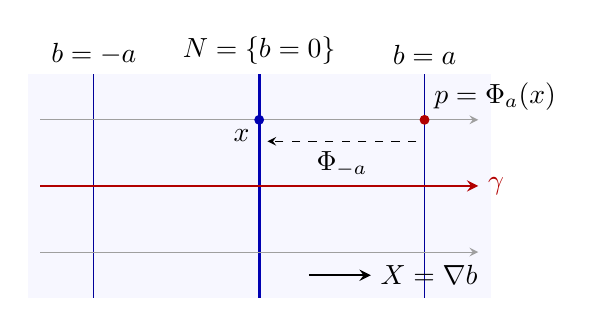
\begin{tikzpicture}[>=stealth,scale=1.05]
	\fill[blue!3] (-2.8,-1.35) rectangle (2.8,1.35);
	\draw[blue!60!black] (-2,-1.35)--(-2,1.35);
	\draw[very thick,blue!70!black] (0,-1.35)--(0,1.35);
	\draw[blue!60!black] (2,-1.35)--(2,1.35);
	\node[above] at (-2,1.35) {\(b=-a\)};
	\node[above] at (0,1.35) {\(N=\{b=0\}\)};
	\node[above] at (2,1.35) {\(b=a\)};
	\draw[->,gray!75] (-2.65,-.8)--(2.65,-.8);
	\draw[->,thick,red!70!black] (-2.65,0)--(2.65,0);
	\node[right,red!70!black] at (2.65,0) {\(\gamma\)};
	\draw[->,gray!75] (-2.65,.8)--(2.65,.8);
	\fill[blue!70!black] (0,.8) circle (1.7pt);
	\fill[red!70!black] (2,.8) circle (1.7pt);
	\node[below left] at (0,.8) {\(x\)};
	\node[above right] at (2,.8) {\(p=\Phi_a(x)\)};
	\draw[->,dashed] (1.9,.54)--(.1,.54);
	\node[below] at (1,.54) {\(\Phi_{-a}\)};
	\draw[->,thick] (.6,-1.08)--(1.35,-1.08);
	\node[right] at (1.35,-1.08) {\(X=\nabla b\)};
\end{tikzpicture}

	\caption[平行梯度流与水平集乘积]{平行梯度流把 \(N=b^{-1}(0)\) 等距地送到各水平集。点 \(p\) 的乘积坐标是 \((b(p),\Phi_{-b(p)}p)\)。图中水平箭头表示流轨道，纵向线表示水平集；它们的平面形状只用于标示相交关系。}
	\label{g3:fig:splitting-flow}
\end{figure}

\begin{example}\label{g3:exm:ray-without-line-paraboloid}
	在 \(\mathbb R^3\) 中取抛物面 \(P=\{z=x^2+y^2\}\)，带诱导度量。用 \((x,y)\) 参数表示，度量为
	\[
		g=\mathrm dx^2+\mathrm dy^2+(2x\,\mathrm dx+2y\,\mathrm dy)^2
		\ge\mathrm dx^2+\mathrm dy^2.
	\]
	因此其内在 Cauchy 列在参数平面中也 Cauchy；参数落在某个有界圆盘内时，\(g\) 又受 Euclid 度量的常数倍控制，所以 Euclid 极限也是内在极限。故 \(P\) 完备，且显然非紧。\cref{g3:lem:complete-noncompact-ray}保证它从每点都有射线。

	取上单位法向 \((-2x,-2y,1)/\sqrt{1+4x^2+4y^2}\)。相应第二基本形式是 \(2(\mathrm dx^2+\mathrm dy^2)/\sqrt{1+4x^2+4y^2}\)，而第一基本形式的行列式为 \(1+4x^2+4y^2\)。Gauss 方程因而给出
	\[
		K=\frac{\det\operatorname{Hess}(x^2+y^2)}
		{(1+|\nabla(x^2+y^2)|^2)^2}
		=\frac4{(1+4x^2+4y^2)^2}>0.
	\]
	二维中 \(\operatorname{Ric}=Kg>0\)。若它有直线，分裂定理就给出 \(P\cong\mathbb R\times N^1\)；但两个一维因子的黎曼乘积曲率为零，与上式矛盾。所以有射线与有直线确有区别。
\end{example}

分裂结论也不能直接从一个覆盖空间下降到商空间。例如 \(\mathbb R^n\) 含有许多直线并可分裂，取格点平移的商却得到紧平坦环面。覆盖投影保持测地线方程与局部长度，却可能使远处两点有更短的连接，因而不保持直线的整体最短性。章末习题还会给出非紧平坦商空间的同类现象。

\ProseParagraphBreak

完备性控制的是另一个步骤。在 \(\mathbb R^2\setminus\{(0,1)\}\) 的 Euclid 度量上，\(b(x,y)=x\) 光滑调和，\(\nabla b=\partial_x\) 平行且长为一，\(x\) 轴也是测地直线。但是从 \((-1,1)\) 出发的梯度轨道在时间一到达被删去的点，不能继续；零水平集也断成两部分。这说明上述流与逆映射的整体构造确实使用了完备性。
% 纲要条目排为编号小节标题，并进入目录与书签；说明段仍保留于纲要注释中。


\begin{chaptersummary}
	Hodge 理论以度量为每个 de Rham 类选出唯一调和代表。Green 算子的两阶正则性增益给出正合、余正合与调和的正交分解；星算子把非零调和形式变成与它积分不为零的互补次数形式，从而得到对偶。代表和 Hodge 内积随度量改变，外积积分配对则由定向与上同调类决定；不可定向情形通过定向线丛保存同一配对结构。

	\ProseParagraphBreak

	Weitzenböck 公式把调和形式的外微分能量改写为协变导数能量与曲率项。一形式上的曲率项是 Ricci 作用，高阶形式需要相应的 \(\mathcal R_q\)。非负性给出平行性，某点的正定性给出消失。离开紧情形以后，距离截断将积分问题化为环带误差；完备性、平方可积性和增长条件各自承担明确的作用。

	\ProseParagraphBreak

	分裂证明把这些工具用在一条测地直线上。两侧 Busemann 函数之和具有内部最大值，弱最大值原理使它恒为零，因而两侧函数各自调和并光滑。沿渐近射线的增长确定梯度长度为一，Bochner 公式使该梯度平行；完整的梯度流最终把流形等距地识别为水平集与实直线的乘积。
\end{chaptersummary}

\BookExercises

\begin{exercise}\label{g3:ex:self-dual-four-forms}
	在定向四维内积空间的正向正交余标架 \(e^1,e^2,e^3,e^4\) 中，求 \(*:\Lambda^2\to\Lambda^2\) 的两个特征空间及正交归一基。再设 \(M\) 为定向闭四维黎曼流形，证明每个实调和二形式唯一分为调和的自对偶与反自对偶部分，并计算 \(\int_M\omega\wedge\omega\)。
\end{exercise}
\begin{solution}
	记 \(e^{ij}=e^i\wedge e^j\)。补指标的排列符号给出
	\[
		*e^{12}=e^{34},\qquad *e^{13}=-e^{24},\qquad
		*e^{14}=e^{23}.
	\]
	因为二形式上 \(*^2=I\)，反方向的三个公式也随之确定。特征值 \(+1\) 的正交归一基为
	\[
		\frac{e^{12}+e^{34}}{\sqrt2},\quad
		\frac{e^{13}-e^{24}}{\sqrt2},\quad
		\frac{e^{14}+e^{23}}{\sqrt2};
	\]
	把每项中的第二个加数变号，便得特征值 \(-1\) 的正交归一基。两空间各三维且互相正交。

	在流形上令 \(\omega_\pm=(\omega\pm *\omega)/2\)。星与 Laplace 交换，所以 \(\omega\) 调和时两个分量都调和；特征空间分解保证唯一。由于 \(\omega_+,\omega_-\) 正交，
	\[
		\omega\wedge\omega
		=\omega_+\wedge *\omega_+
		-\omega_-\wedge *\omega_-
		=(|\omega_+|^2-|\omega_-|^2)\operatorname{vol}_g.
	\]
	于是所求积分为 \(\|\omega_+\|_2^2-\|\omega_-\|_2^2\)。中间次数的外积配对在这两个调和子空间上分别正定、负定；它与始终正定的 Hodge 内积不同。
\end{solution}

\begin{exercise}\label{g3:ex:explicit-torus-hodge-pieces}
	在标准平坦环面 \((\mathbb R/2\pi\mathbb Z)^2\) 上，对
	\[
		\omega=(2+\cos x)\,\mathrm dx+(-1+\sin x)\,\mathrm dy
	\]
	求调和、正合与余正合分量，并求 \(\delta G_1\omega\)、\(\mathrm dG_1\omega\)。计算三个分量各自的平方 \(L^2\) 范数。
\end{exercise}
\begin{solution}
	平坦环面上的调和形式系数为常数，故
	\(h=2\,\mathrm dx-\mathrm dy\)。
	其余两个分量可直接写成
	\[
		\mathrm d(\sin x)=\cos x\,\mathrm dx,\qquad
		\delta(\cos x\,\mathrm dx\wedge\mathrm dy)=\sin x\,\mathrm dy.
	\]
	二者都具有零平均系数，且它们与 \(h\) 及彼此正交，故这就是 Hodge 分解。

	Laplace 逐分量作用为 \(-\partial_x^2-\partial_y^2\)，所以
	\[
		G_1\omega=\cos x\,\mathrm dx+\sin x\,\mathrm dy,
		\qquad
		\delta G_1\omega=\sin x,\qquad
		\mathrm dG_1\omega=\cos x\,\mathrm dx\wedge\mathrm dy.
	\]
	这里 Green 解的系数均零平均，确实正交于调和核。环面面积为 \(4\pi^2\)，而 \(\int_0^{2\pi}\cos^2x\,\mathrm dx=\int_0^{2\pi}\sin^2x\,\mathrm dx=\pi\)，故三个平方范数分别为
	\(20\pi^2,2\pi^2,2\pi^2\)，总和为 \(24\pi^2\)。
\end{solution}

\begin{exercise}\label{g3:ex:conformal-middle-hodge}
	设 \(M^n\) 为定向闭黎曼流形，\(\widetilde g=e^{2\varphi}g\)，其中 \(\varphi\) 为实光滑函数。证明在 \(k\) 形式上
	\[
		*_{\widetilde g}=e^{(n-2k)\varphi}*_g.
	\]
	当 \(n=2k\) 时，证明两度量的调和 \(k\) 形式空间相同，且这些形式的 \(L^2\) 内积相同。说明这一结论为何不意味着所有次数的调和代表都不变。
\end{exercise}
\begin{solution}
	余切向量的内积乘以 \(e^{-2\varphi}\)，所以 \(k\) 形式内积乘以 \(e^{-2k\varphi}\)；体积形式乘以 \(e^{n\varphi}\)。代入星的定义，由外积配对的非退化性得到所求公式。同时
	\[
		(\alpha,\beta)_{\widetilde g}
		=\int_M e^{(n-2k)\varphi}\langle\alpha,\beta\rangle_g\,\mu_g.
	\]
	在中间次数上，这个内积不变。

	若 \(n=2k\)，内侧作用于 \(k\) 形式的星不变，而外侧作用于 \(k+1\) 形式的星乘以 \(e^{-2\varphi}\)，因此
	\(\delta_{\widetilde g}\alpha=e^{-2\varphi}\delta_g\alpha\)。
	外微分本来就与度量无关。闭流形上的调和条件等价于 \(\mathrm d\alpha=\delta\alpha=0\)，故两种调和空间相同。其他次数中，内侧星的比例因子一般不是常数，外微分会对它求导；例如正文中非恒定共形环面的调和顶次形式由常系数 \(\mathrm dx\wedge\mathrm dy\) 变成 \(e^{2\varphi}\mathrm dx\wedge\mathrm dy\) 的常数倍。
\end{solution}

\begin{exercise}\label{g3:ex:circle-pullback-projection}
	两圆周都带标准度量 \(\mathrm d\theta^2\)。给定整数 \(m\ge1\) 及 \(0<|\varepsilon|<m\)，令
	\[
		F([\theta])=[m\theta+\varepsilon\sin\theta].
	\]
	证明 \(F\) 是 \(m\) 重光滑覆盖，计算 \(F^*(\mathrm d\theta)\) 的调和代表。它本身是否调和？若将源圆周的度量改为 \(F^*(\mathrm d\theta^2)\)，答案如何变化？
\end{exercise}
\begin{solution}
	实直线上的提升 \(\widetilde F(\theta)=m\theta+\varepsilon\sin\theta\) 满足
	\(\widetilde F(\theta+2\pi)=\widetilde F(\theta)+2m\pi\)，故下降为圆周映射。其导数 \(m+\varepsilon\cos\theta>0\)，且提升严格递增、从 \(-\infty\) 走到 \(+\infty\)。在一周期内，每个模 \(2\pi\) 的值恰有 \(m\) 个原像；逆函数定理在每个原像附近给出局部光滑逆，因而是 \(m\) 重覆盖。

	拉回为
	\[
		F^*(\mathrm d\theta)
		=(m+\varepsilon\cos\theta)\,\mathrm d\theta
		=m\,\mathrm d\theta+\mathrm d(\varepsilon\sin\theta).
	\]
	标准度量下，一形式调和当且仅当系数为常数，所以它不调和，调和代表为 \(m\,\mathrm d\theta\)。新度量为 \(a^2\mathrm d\theta^2\)，其中 \(a=m+\varepsilon\cos\theta>0\)。此时拉回恰为 \(a\,\mathrm d\theta\)，由余微分公式立即得到它调和。这个局部等距的拉回现象与普通光滑拉回后需要调和投影的情形相符。
\end{solution}

\begin{exercise}\label{g3:ex:sphere-top-form-primitive}
	设 \(S^2\subset\mathbb R^3\) 为单位球面，带标准度量和外法向定向，\(z\) 为第三坐标限制。求方程
	\[
		\Delta_2 u=z\,\operatorname{vol}_{S^2}
	\]
	唯一正交于调和核的解，并为 \(z\,\operatorname{vol}_{S^2}\) 写出一个全局光滑原像。若右端改为 \((1+z)\operatorname{vol}_{S^2}\)，方程是否可解？
\end{exercise}
\begin{solution}
	球面梯度为 \(\nabla z=e_3-zx\)。沿球面切向量 \(X\) 求环境导数并取切向部分，得
	\(\nabla_X\nabla z=-zX\)，故 \(\operatorname{Hess}z=-zg\)、\(\Delta_0z=2z\)。反射对称性给出 \(\int_{S^2}z\,\mu_g=0\)。
	星与 Laplace 交换，因此
	\[
		u=\frac12z\,\operatorname{vol}_{S^2}
	\]
	满足方程。调和顶次形式是体积形式的常数倍，上述零积分保证 \(u\) 正交于它们，所以解具有所要求的唯一性。

	令 \(\eta=\delta u=-\tfrac12*\mathrm dz\)。由于 \(\mathrm du=0\)，有
	\(\mathrm d\eta=\Delta_2u=z\,\operatorname{vol}_{S^2}\)。
	它的光滑性已由整体星算子保证；在球坐标 \(z=\cos\theta\) 中还可写成
	\[
		\eta=\frac12\sin^2\theta\,\mathrm d\phi
		=\frac12(x\,\mathrm dy-y\,\mathrm dx)\big|_{S^2},
	\]
	最后一个表达式直接说明极点处没有奇性。若改用右端 \((1+z)\operatorname{vol}_{S^2}\)，它与调和体积形式的内积为 \(4\pi\ne0\)，不满足 Green 可解条件，故无解。
\end{solution}

\begin{exercise}\label{g3:ex:torus-two-pairings}
	在 \(T^2=(\mathbb R/2\pi\mathbb Z)^2\) 上取定向 \(\mathrm dx\wedge\mathrm dy\) 及度量
	\(g=a^2\mathrm dx^2+b^2\mathrm dy^2\)，其中 \(a,b>0\) 为常数。在 \(H_{\mathrm{dR}}^1(T^2;\mathbb R)\) 的基 \([\mathrm dx],[\mathrm dy]\) 中，分别计算外积积分配对、Hodge 内积及星算子的矩阵。解释前者与后两者对 \(a,b\) 的依赖为何不同。
\end{exercise}
\begin{solution}
	系数恒定的形式 \(\mathrm dx,\mathrm dy\) 调和，且由平坦环面的 Hodge 计算构成一阶上同调基。正交余标架为 \(a\,\mathrm dx,b\,\mathrm dy\)，所以
	\[
		*\mathrm dx=\frac ba\,\mathrm dy,\qquad
		*\mathrm dy=-\frac ab\,\mathrm dx.
	\]
	以输入向量的像作为矩阵列，星矩阵为
	\[
		S=\begin{pmatrix}0&-a/b\\ b/a&0\end{pmatrix}.
	\]
	积分 \(\int_{T^2}\mathrm dx\wedge\mathrm dy=4\pi^2\)，故外积配对矩阵为
	\[
		I=4\pi^2\begin{pmatrix}0&1\\-1&0\end{pmatrix}.
	\]
	Hodge 内积满足 \((\alpha,\beta)=\int\alpha\wedge *\beta\)，所以其矩阵为
	\[
		G=IS=4\pi^2\begin{pmatrix}b/a&0\\0&a/b\end{pmatrix}.
	\]
	外积积分只用定向和上同调类；度量决定互补方向的长度比例，从而改变星与正定内积。这里 \(S^2=-I_2\)，而 \(IS\) 正定，亦与一形式星的平方及配对公式一致。
\end{solution}

\begin{exercise}\label{g3:ex:ricci-eigenvalue-bound}
	设 \(M^n\) 为连通闭黎曼流形，\(n\ge2\)，且
	\(\operatorname{Ric}\ge(n-1)\kappa g\)，其中 \(\kappa>0\)。
	\begin{enumerate}
		\item 证明对任意实光滑函数 \(f\)，有
		\[
			\int_M(\Delta f)^2\,\mu_g
			=\int_M|\operatorname{Hess}f|^2\,\mu_g
			 +\int_M\operatorname{Ric}(\nabla f,\nabla f)\,\mu_g.
		\]
		\item 若 \(f\ne0\)、\(\Delta f=\lambda f\)、\(\lambda>0\)，证明
		\(\lambda\ge n\kappa\)。若取等，证明
		\(\operatorname{Hess}f=-\kappa f\,g\)。
		\item 在单位圆球 \(S^n\) 上用坐标函数验证下界达到。
	\end{enumerate}
\end{exercise}
\begin{solution}
	1. 对函数 Bochner 公式积分，左侧的散度积分为零，而
	\[
		\int_M\langle\nabla\Delta f,\nabla f\rangle\,\mu_g
		=\int_M(\Delta f)^2\,\mu_g.
	\]
	移项即得恒等式。

	2. 对称矩阵的迹不等式给出
	\[
		|\operatorname{Hess}f|^2
		\ge\frac1n(\operatorname{tr}\operatorname{Hess}f)^2
		=\frac1n(\Delta f)^2.
	\]
	又有 \(\int|\nabla f|^2=\lambda\int f^2\)。因此
	\[
		\lambda^2\int f^2
		\ge\frac{\lambda^2}{n}\int f^2
		    +(n-1)\kappa\lambda\int f^2.
	\]
	除以正数 \((n-1)\lambda\int f^2\)，得到
	\(\lambda/n\ge\kappa\)。若 \(\lambda=n\kappa\)，则上述两项非负误差的积分都为零，特别是
	\[
		\operatorname{Hess}f
		=\frac{\operatorname{tr}\operatorname{Hess}f}{n}g
		=-\frac{\lambda f}{n}g=-\kappa f\,g
	\]
	逐点成立。

	3. 在 \(S^n\subset\mathbb R^{n+1}\) 上取 \(f(x)=x_{n+1}\)，并以
	\(E=(0,\ldots,0,1)\) 表示环境常向量。切向梯度为
	\(\nabla f=E-fx\)。对切向量 \(X\) 求环境导数再投到切空间，
	\[
		\nabla_X\nabla f
		=\bigl(-X(f)x-fX\bigr)^\top=-fX.
	\]
	故 \(\operatorname{Hess}f=-fg\)，取负迹得 \(\Delta f=nf\)。
	单位圆球的 Ricci 曲率为 \((n-1)g\)，所以 \(\kappa=1\) 时下界取等。
\end{solution}

\begin{exercise}\label{g3:ex:parallel-forms-sphere-circle}
	给 \(M=S^2\times S^1\) 配单位圆球与长度 \(2\pi\) 圆周的乘积度量。记
	\(\vartheta\) 为圆周上的标准平行一形式，\(\sigma\) 为圆球的面积形式，并沿投影拉回到 \(M\)。求各阶实调和形式，证明它们分别由
	\[
		1,\qquad \vartheta,\qquad \sigma,\qquad
		\sigma\wedge\vartheta
	\]
	张成。说明这里 Ricci 非负为何没有给出一阶消失。
\end{exercise}
\begin{solution}
	乘积联络保持两个因子的分布。圆球切平面的曲率算子为一，含圆周方向的混合二向量曲率为零，所以整个曲率算子非负。因此各阶调和形式均平行。

	对调和一形式 \(\alpha\)，令 \(X=\alpha^\sharp\)。它满足
	\(\operatorname{Ric}(X,X)=0\)。乘积的 Ricci 二次型为
	\[
		\operatorname{Ric}(X,X)=|X_{S^2}|^2,
	\]
	故 \(X\) 只能沿圆周方向，\(\alpha=h\vartheta\)。
	因为 \(\alpha,\vartheta\) 都平行且 \(\vartheta\) 无零点，得到
	\(\mathrm dh=0\)，连通性给出 \(h\) 为常数。因此
	\(\mathcal H^1(M)=\mathbb R\vartheta\)。

	取乘积定向。Hodge 星保持平行性并在一形式与二形式间给出同构，而
	\(*\vartheta=\sigma\)，故 \(\mathcal H^2(M)=\mathbb R\sigma\)。
	零阶调和函数平行，因而为常数；星再给出
	\(\mathcal H^3(M)=\mathbb R(\sigma\wedge\vartheta)\)。
	这些列出的形式确实都平行，所以同时证明了包含关系的另一方向。

	Ricci 在每一点的圆周方向上都为零，因此没有任何一点使其正定。一阶形式 \(\vartheta\) 恰好处于这一零方向中。它的圆周积分为 \(2\pi\)，所以其上同调类非零。
\end{solution}

\begin{exercise}\label{g3:ex:flat-quotient-parallel-invariants}
	在 Euclid 平面上令
	\[
		a(x,y)=(x+1,y),\qquad b(x,y)=(-x,y+1),
	\]
	并令 \(\Gamma\) 为它们生成的等距变换群。证明
	\(M=\mathbb R^2/\Gamma\) 是连通闭平坦曲面，并求其全部实调和形式。由此说明平坦性不保证 \(b_1(M)=\dim M\)。
\end{exercise}
\begin{solution}
	关系 \(bab^{-1}=a^{-1}\) 说明每个群元素可唯一写成
	\(a^m b^k\)，作用为
	\[
		a^m b^k(x,y)=((-1)^k x+m,y+k),
		\qquad m,k\in\mathbb Z.
	\]
	若 \(k\ne0\)，其第二坐标发生非零平移；若 \(k=0,m\ne0\)，第一坐标发生非零平移。因此非恒等元素均无不动点。对任意紧集，只有有限个整数 \(m,k\) 能使其像与原紧集相交，所以作用适当不连续，商为光滑无边界曲面，平坦度量下降。先用 \(b\) 的幂把 \(y\) 移入 \([0,1]\)，再用 \(a\) 的幂把 \(x\) 移入 \([0,1]\)，可见紧矩形的像覆盖商空间，故商紧。连通性从 \(\mathbb R^2\) 继承。

	曲率项恒为零，所以调和形式恰为平行形式。将其提升到 \(\mathbb R^2\)，平行性意味着它在标准余标架中的系数为常数；下降的条件恰是 \(\Gamma\) 不变性。平移 \(a\) 不改变这些常系数形式，而
	\[
		b^*\mathrm dx=-\mathrm dx,\qquad
		b^*\mathrm dy=\mathrm dy,\qquad
		b^*(\mathrm dx\wedge\mathrm dy)
		   =-\mathrm dx\wedge\mathrm dy.
	\]
	故零阶调和空间为 \(\mathbb R\)，一阶由下降的 \(\mathrm dy\) 张成，二阶为零。于是
	\(b_0=1,b_1=1,b_2=0\)。平坦度量的环路平行移动仍可翻转一个方向；平行一形式必须同时保留这一信息，所以其维数可以小于二。该曲面非定向，其 Poincar\'e 配对应像式\eqref{g3:eq:twisted-poincare-pairing}那样使用定向线丛，不能要求普通实系数的零阶与顶阶维数相等。
\end{solution}

\begin{exercise}\label{g3:ex:bochner-cohomology-subalgebra}
	设 \(M^n\) 为连通闭黎曼流形。
	\begin{enumerate}
		\item 若 \(\operatorname{Ric}\ge0\)、\(r=b_1(M)\)，证明由外积诱导的分次代数映射
		\[
			\Lambda^*H_{\mathrm{dR}}^1(M;\mathbb R)
			\longrightarrow H_{\mathrm{dR}}^*(M;\mathbb R)
		\]
		为单射。因此 \(b_q(M)\ge\binom rq\)，其中 \(0\le q\le r\)。
		\item 若曲率算子 \(\mathcal R\ge0\)，证明对每个 \(p\in M\)，将上同调类先取调和代表再在 \(p\) 求值，给出分次代数单射
		\[
			H_{\mathrm{dR}}^*(M;\mathbb R)
			\longrightarrow\Lambda^*\mathrm T_p^*M.
		\]
	\end{enumerate}
\end{exercise}
\begin{solution}
	1. 取 \(H_{\mathrm{dR}}^1\) 的一组基的调和代表
	\(\alpha_1,\ldots,\alpha_r\)。Ricci 非负使它们全部平行。固定一点 \(p\)；求值映射在平行形式上单射，因此
	\(\alpha_1(p),\ldots,\alpha_r(p)\) 线性无关。相应的
	\(\binom rq\) 个外积在 \(\Lambda^q\mathrm T_p^*M\) 中线性无关。

	每个全局外积
	\(\alpha_{i_1}\wedge\cdots\wedge\alpha_{i_q}\) 都平行，因而调和。若这些形式的某个线性组合代表零上同调类，则它作为调和代表只能为零；在 \(p\) 求值，得到全部系数为零。因此每个次数上的映射均单射。外积与上同调乘法的定义相容，故所得映射是分次代数单射，并得到维数下界。

	2. 曲率算子非负使所有次数的调和形式都平行，所以两个调和形式的外积仍平行且调和。它代表两个原上同调类的乘积，故由唯一性，这个外积就是乘积类的调和代表。于是取调和代表成为分次代数同构到调和形式组成的子代数。求值显然保持外积，且在每个次数的平行形式空间上单射，复合即为所求。通常调和形式的外积未必调和；这里使乘法相容的具体原因是平行性。
\end{solution}

\begin{exercise}\label{g3:ex:incomplete-cutoff-obstruction}
	在不完备流形 \((0,1)\) 上取 Euclid 度量。证明若 \(\chi\) 紧支、Lipschitz 且 \(\chi(1/2)=1\)，则 \(\|\chi'\|_{L^\infty}\ge2\)。据此说明不能存在局部最终等于一而梯度范数趋零的紧支截断族。用 \(u(x)=x\) 检验不完备情形下 \(L^2\) 分布调和函数未必为常数，并指出对它直接使用全空间能量恒等式错在哪里。
\end{exercise}
\begin{solution}
	紧支性使某个 \(a\in(0,1/2)\) 满足 \(\chi(a)=0\)。绝对连续性给出
	\[
		1=|\chi(1/2)-\chi(a)|
		\le(1/2-a)\|\chi'\|_\infty,
	\]
	因此 \(\|\chi'\|_\infty\ge(1/2-a)^{-1}>2\)，尤其有题设下界。局部最终等于一的族必定在 \(1/2\) 处最终取值一，故梯度范数不可能趋零。

	函数 \(u=x\) 满足 \(-u''=0\) 且 \(\int_0^1u^2=1/3<\infty\)，但 \(u'=1\)。它在 \((0,1)\) 内的分布方程只允许紧支测试，不能将 \(u\) 本身直接当作紧支测试函数。若在闭区间上计算，真正的公式是
	\[
		0=\int_0^1(-u'')u
		=\int_0^1|u'|^2-[u'u]_0^1=1-1.
	\]
	被漏掉的端点通量恰好抵消梯度能量；紧支截断的导数无法趋零，反映了同一个障碍。
\end{solution}

\begin{exercise}\label{g3:ex:subquadratic-harmonic-growth}
	设 \((M,g)\) 非空、连通、完备、光滑且无边界，并有
	\(\operatorname{Vol}B_R(o)\le CR^\nu\) 对 \(R\ge1\) 成立，其中 \(\nu\ge0\)。设弱调和函数 \(u\in H^1_{\mathrm{loc}}(M;\mathbb R)\) 满足
	\[
		|u(x)-a|\le C(1+d(o,x))^\alpha
	\]
	几乎处处，其中 \(a\in\mathbb R\)、\(\alpha\ge0\)。证明若 \(2\alpha+\nu<2\)，则 \(u\) 为常数。将结论应用于平坦圆柱上的有界调和函数，并解释为什么圆柱上的非零平行一形式 \(\mathrm d\theta\) 满足式\eqref{g3:eq:harmonic-form-annular-growth}却不属于 \(L^2\)。
\end{exercise}
\begin{solution}
	在 \(A_R\) 上，增长界给出 \(|u-a|^2\le C'(1+2R)^{2\alpha}\)。所以
	\[
		R^{-2}\int_{A_R}|u-a|^2\,\mu_g
		\le C''R^{2\alpha+\nu-2}\longrightarrow0.
	\]
	\Cref{g3:prop:complete-harmonic-caccioppoli}遂给出常数结论；其连续光滑代表由\cref{g3:prop:weak-harmonic-smoothing}确定。

	在 \(S^1\times\mathbb R\) 上取 \(\mathrm d\theta^2+\mathrm dt^2\)，圆周长度为 \(2\pi\)。以 \((1,0)\) 为球心，距离球包含于 \(S^1\times(-R,R)\)，故体积至多 \(4\pi R\)。因此可取 \(\nu=1\)；有界调和函数可取 \(a=0,\alpha=0\)，满足严格不等式。

	一形式 \(\mathrm d\theta\) 的长度恒为一，平行，因而调和。其环带平方积分至多为 \(8\pi R\)，乘 \(R^{-2}\) 后趋零；但全圆柱体积无限，所以它不平方可积。这说明环带增长条件能适用于某些非 \(L^2\) 形式，而其结论只是闭、余闭或在曲率条件下平行，不能据此自动推出消失。
\end{solution}

\begin{exercise}\label{g3:ex:hyperbolic-disk-exact-l2-forms}
	在单位圆盘 \(D\subset\mathbb C\) 上取
	\[
		g=\frac{4}{(1-|z|^2)^2}(\mathrm dx^2+\mathrm dy^2).
	\]
	证明该度量完备。对整数 \(m\ge1\)，令 \(f_m(z)=\operatorname{Re}z^m\)、\(\omega_m=\mathrm df_m\)。证明 \(\omega_m\) 是非零的 \(L^2\) 调和一形式，计算 \(\|\omega_m\|_2^2\)，并证明不同 \(m\) 对应的形式两两正交。说明这些形式在普通 de Rham 上同调中的类，以及为何这不与非负曲率项下的消失结论矛盾。
\end{exercise}
\begin{solution}
	写 \(\lambda=2/(1-r^2)\)。任意从原点到半径 \(r\) 处的道路，其长度至少为
	\[
		\int_0^r\frac{2\,\mathrm ds}{1-s^2}
		=\log\frac{1+r}{1-r},
	\]
	因为沿道路有 \(|\dot r|\le|\dot z|\)；径向线段达到此长度。因此有界距离球留在 Euclid 半径严格小于一的闭盘中。该闭盘上度量与 Euclid 度量一致可比，距离闭球是紧集。Hopf--Rinow 定理给出完备性。

	二维坐标公式为
	\[
		\Delta_g f=-\lambda^{-2}(\partial_x^2f+\partial_y^2f).
	\]
	\(f_m\) 是 Euclid 调和多项式，故 \(\Delta_gf_m=0\)。于是
	\(\mathrm d\omega_m=0\)、\(\delta_g\omega_m=\Delta_gf_m=0\)，从而 \(\Delta_1\omega_m=0\)。一形式的平方长度贡献 \(\lambda^{-2}\)，密度贡献 \(\lambda^2\)，故它们相消：
	\[
		\|\omega_m\|_{L^2(g)}^2
		=\int_D|\mathrm df_m|_{\mathrm{Eucl}}^2\,\mathrm dx\mathrm dy
		=\int_0^{2\pi}\!\int_0^1m^2r^{2m-2}r\,\mathrm dr\mathrm d\theta
		=\pi m.
	\]
	对 \(m\ne\ell\)，梯度配对的角向因子为 \(\cos((m-\ell)\theta)\)，其积分为零，所以各形式两两正交。这已经给出一个无限的线性无关族。

	每个 \(\omega_m=\mathrm df_m\) 都是全局正合形式，因此其普通 de Rham 类为零；非零 \(L^2\) 调和形式不能在非紧情形中仅凭普通上同调类判定。该度量的 Gauss 曲率为负一：用 \(K=-\lambda^{-2}(\partial_x^2+\partial_y^2)\log\lambda\)，其中 \((\partial_x^2+\partial_y^2)\log\lambda=4/(1-r^2)^2\)，即可核对。二维的一形式曲率项为 Ricci 作用，故 \(\mathcal R_1=-I\)，不满足非负假设。
\end{solution}

\begin{exercise}\label{g3:ex:weak-subharmonic-limit-hypotheses}
	说明以下两点。
	\begin{enumerate}
		\item 在 \(\mathbb R^n\)、\(n\ge3\)，函数 \(u(x)=-(1+|x|^2)^{-(n-2)/2}\) 是有界、非恒定的光滑次调和函数。本书采用 \(\Delta=-\sum_i\partial_i^2\)，请计算其 \(\Delta u\) 并解释它为何不违背强最大值原理。
		\item 在 \(\mathbb R\) 上，将零函数仅在原点改成取值一。所得点态函数与零函数代表同一个 \(H^1_{\mathrm{loc}}\) 元素，且分布调和，却在原点有严格最大值。解释强最大值定理为什么要指定连续代表。
	\end{enumerate}
\end{exercise}
\begin{solution}
	（1）令 \(r=|x|\)、\(a=(n-2)/2\)。对 \(v=(1+r^2)^{-a}\)，径向求导给出
	\[
		v''+\frac{n-1}{r}v'
		=-n(n-2)(1+r^2)^{-(n+2)/2}.
	\]
	此式在原点按光滑延拓理解。由于 \(u=-v\)，有
	\[
		\Delta u=-n(n-2)(1+|x|^2)^{-(n+2)/2}<0.
	\]
	所以 \(u\) 次调和，取值于 \([-1,0)\)，而上确界零仅在趋向无穷远时逼近，没有在内部达到。强最大值原理的接触假设不满足。

	（2）改变零测集上的取值不改变任何测试积分或弱导数，所以这个点态函数的分布 Laplace 仍为零。其唯一连续调和代表是处处为零的函数，而所给的特殊点态代表不连续。强最大值结论比较的是指定连续代表的点值；若允许任意修改零测集上的值，内部极值就不再由弱方程决定。
\end{solution}

\begin{optionalexercise}\label{g3:ex:hyperbolic-busemann-failure}
	在双曲上半平面 \(\mathbb H^2=\{(x,y):y>0\}\) 上取度量 \(g=y^{-2}(\mathrm dx^2+\mathrm dy^2)\) 与直线 \(\gamma(t)=(0,e^t)\)。采用本书的 Busemann 符号与 \(\Delta=-\operatorname{div}\nabla\)。计算 \(b_+,b_-\) 及 \(\Delta b_\pm\)，验证 \(b_++b_-\le0\) 在线上取等号，却不恒为零，并指出分裂证明中的哪一项假设失效。计算中可以使用上半平面反演的等距性，但须核对它。
\end{optionalexercise}
\begin{solution}
	任意连接两点的曲线满足
	\[
		L_g(c)\ge\int\frac{|y'|}{y}\,\mathrm ds
		\ge|\log y_1-\log y_0|.
	\]
	竖直曲线达到这个下界，所以 \(\gamma\) 确为单位速直线。固定 \((x,y)\)，当 \(T>\log y\) 时，先沿竖直方向走到 \((x,e^T)\)，再水平走到 \((0,e^T)\)，得到
	\[
		T-\log y\le d_g((x,y),\gamma(T))
		\le T-\log y+|x|e^{-T}.
	\]
	因此 \(b_+(x,y)=\log y\)。

	令
	\[
		I(x,y)=\left(-\frac{x}{x^2+y^2},\frac{y}{x^2+y^2}\right).
	\]
	写成复变量就是 \(I(z)=-1/z\)，故 Euclid 长度被乘以 \(|z|^{-2}\)，新高度也等于 \(y|z|^{-2}\)，两者之比不变。因此 \(I^*g=g\)。它又满足 \(I(\gamma(-T))=\gamma(T)\)，所以
	\[
		b_-(x,y)=b_+(I(x,y))
		=\log\frac{y}{x^2+y^2}.
	\]
	于是
	\[
		b_++b_-=
		\log\frac{y^2}{x^2+y^2}\le0,
	\]
	等号恰在 \(x=0\) 时成立。

	二维共形度量的散度坐标式直接给出
	\(\Delta=-y^2(\partial_x^2+\partial_y^2)\)。从而 \(\Delta\log y=1\)；\(\log(x^2+y^2)\) 在上半平面是 Euclid 调和函数，也可由等距性得 \(\Delta b_-=1\)。所以
	\[
		\Delta(b_++b_-)=2>0.
	\]
	这里和函数是本书符号下的弱超调和函数，不能对它使用弱次调和的强最大值原理。双曲度量有 \(K=-1\)，从而 \(\operatorname{Ric}=-g\)；失效的正是 Ricci 非负条件，而直线与完备性均成立。
\end{solution}

\begin{optionalexercise}\label{g3:ex:flat-mobius-no-line}
	令 \(G:\mathbb R^2\to\mathbb R^2\) 为 \(G(x,y)=(x+1,-y)\)，并给商空间
	\[
		M=\mathbb R^2/\langle G\rangle
	\]
	赋予使投影局部等距的平坦度量。证明 \(M\) 光滑、无边界、完备且非紧，并显式给出一条射线；再证明 \(M\) 没有测地直线。由此说明在非紧情形，万有覆盖中的等距 \(\mathbb R\) 因子也可能不能下降到商空间。
\end{optionalexercise}
\begin{solution}
	有 \(G^k(x,y)=(x+k,(-1)^ky)\)。非零整数 \(k\) 改变 \(x\) 坐标，所以作用自由；对两个固定紧集，只有有限个整数平移能使其相交。因此作用适当不连续。每个半径小于 \(1/3\) 的 Euclid 小球与其非平凡平移不交，投影在这样的球上给出局部等距坐标，于是商是光滑无边界平坦流形。

	Euclid 覆盖空间完备，\cref{g3:prop:riemannian-covering-distance}给出商的完备性及距离公式
	\[
		d_M([p],[q])=\min_{k\in\mathbb Z}|p-G^kq|.
	\]
	函数 \(|y|\) 下降到商上且无界，故 \(M\) 非紧。曲线 \(\eta(t)=[(0,t)]\)、\(t\ge0\)，是一条射线：对 \(s,t\ge0\)，偶数 \(k\) 给出的距离平方是 \(k^2+(s-t)^2\)，奇数 \(k\) 给出 \(k^2+(s+t)^2\)。它们均不小于 \((s-t)^2\)，且 \(k=0\) 达到该值。

	另一方面，商上的任意单位速全时测地线都能提升为 Euclid 单位速直线
	\[
		\widetilde\sigma(t)=(at+b,ct+d),\qquad a^2+c^2=1.
	\]
	对任意 \(T>0\)，选奇数 \(k_T\) 使 \(|2aT+k_T|\le1\)。则
	\[
		\bigl|\widetilde\sigma(-T)-G^{k_T}\widetilde\sigma(T)\bigr|^2
		=(2aT+k_T)^2+4d^2\le1+4d^2.
	\]
	因此其投影两端的距离有与 \(T\) 无关的上界，而参数长度为 \(2T\)。充分大的 \(T\) 使该段不再最短，所以不存在测地直线。任意 \(\mathbb R\times N\) 都含有直线，故 \(M\) 不可能有这样的整体等距分解，尽管其万有覆盖就是可分裂的 \(\mathbb R^2\)。
\end{solution}

\begin{optionalexercise}\label{g3:ex:several-harmonic-functions-splitting}
	设 \((M^n,g)\) 连通、完备、光滑、无边界且 \(\operatorname{Ric}\ge0\)。设 \(1\le k\le n\)，\(f_1,\ldots,f_k\) 为实值光滑调和函数，满足 \(\sum_{i=1}^k|\nabla f_i|^2\) 为常数，并且 \((\nabla f_i)\) 在某一点线性无关。证明 \(M\) 等距于 \(\mathbb R^k\times N\)，其中 \(N\) 连通完备且具有非负 Ricci 曲率。说明为什么只假定存在 \(k\) 个线性无关的平行向量场还不足以得到这个结论。
\end{optionalexercise}
\begin{solution}
	对每个 \(f_i\) 使用函数 Bochner 公式并求和。总梯度平方为常数，调和性又消去 \(\nabla\Delta f_i\)，得到
	\[
		0=-\sum_i|\operatorname{Hess}f_i|^2
		-\sum_i\operatorname{Ric}(\nabla f_i,\nabla f_i).
	\]
	每个被减去的量都非负，故每个 \(X_i=\nabla f_i\) 平行。Gram 矩阵 \(C=(\langle X_i,X_j\rangle)\) 因而在连通的 \(M\) 上恒定；一点处的线性无关使它正定。对函数向量施加常矩阵 \(C^{-1/2}\)，再减去某一点的函数值，可得到函数 \(u_1,\ldots,u_k\)，其梯度 \(Y_i\) 处处正交归一，且有共同零点。

	每个 \(Y_i\) 都有全时等距流 \(\Phi^{(i)}\)：长度为一与完备性保证全时存在，平行性保证保持度量。又有
	\[
		[Y_i,Y_j]=\nabla_{Y_i}Y_j-\nabla_{Y_j}Y_i=0.
	\]
	沿第 \(i\) 个流推前 \(Y_j\) 时向量场保持不变，积分曲线唯一性遂使这些流两两交换。由于 \(\mathrm du_j(Y_i)=\delta_{ij}\)，共同水平集
	\(N=\{u_1=\cdots=u_k=0\}\) 是非空的光滑余维 \(k\) 子流形。定义
	\[
		F(t,x)=\Phi_{t_1}^{(1)}\circ\cdots\circ\Phi_{t_k}^{(k)}(x).
	\]
	它满足 \(u_i(F(t,x))=t_i\)，而逆映射为
	\[
		p\longmapsto\left(
		(u_1(p),\ldots,u_k(p)),\,
		\Phi_{-u_1(p)}^{(1)}\circ\cdots\circ
		\Phi_{-u_k(p)}^{(k)}(p)\right).
	\]
	两式光滑且互逆，给出全局微分同胚。各个流等距并保持 \(Y_i\)，而 \(TN\) 是它们的共同正交补，所以
	\[
		g(\mathrm dF(a,v),\mathrm dF(c,w))
		=\sum_{i=1}^k a_ic_i+g_N(v,w).
	\]
	于是 \(F\) 等距。逆映射的第二分量是从连通 \(M\) 到 \(N\) 的满射，故 \(N\) 连通。\(N\) 是闭水平集；乘积投影不增加长度，因此其内在距离等于 \(M\) 距离的限制，完备性随之得到。乘积曲率公式给出 \(\operatorname{Ric}_N\ge0\)。若 \(k=n\)，连通的零维 \(N\) 就是一个点。

	平坦环面有 \(n\) 个线性无关的平行向量场，却不能等距于 \(\mathbb R^n\)。它们的对偶一形式有非零周期，并非全局实值函数的微分；本题给定的 \(f_i\) 排除了这个整体障碍。
\end{solution}

\begin{optionalexercise}\label{g3:ex:two-ends-splitting}
	设 \((M^n,g)\) 连通、完备、光滑、无边界且 \(\operatorname{Ric}\ge0\)。若存在紧集 \(K\subset M\)，使 \(M\setminus K\) 至少有两个无界连通分支，证明 \(M\) 等距于 \(\mathbb R\times N\)，其中 \(N\) 紧。提示：先连接不同分支中趋于无穷远的点，并把最短测地线经过 \(K\) 的时刻移到零。
\end{optionalexercise}
\begin{solution}
	固定 \(o\in M\)，在两个无界分支 \(U,V\) 中分别取 \(p_j,q_j\)，使 \(d(o,p_j),d(o,q_j)\to\infty\)。由完备性，存在连接 \(p_j,q_j\) 的单位速最短测地线。它必须经过 \(K\)：否则其连通像将包含在 \(M\setminus K\) 的同一个连通分支中，不能连接 \(U\) 与 \(V\)。取一个交点 \(z_j\in K\)，以此为参数零点，将曲线记为
	\[
		\sigma_j:[-a_j,b_j]\to M,
		\qquad \sigma_j(0)=z_j.
	\]
	若 \(C=\max_{z\in K}d(o,z)\)，则
	\[
		a_j=d(p_j,z_j)\ge d(o,p_j)-C\to\infty,
		\qquad b_j\to\infty.
	\]
	紧集 \(K\) 上的单位切球丛是紧的，可用有限个局部正交标架与单位球面的紧性验证。取子列使 \((z_j,\dot\sigma_j(0))\to(z,v)\)。完备性与测地线初值的光滑依赖给出全时极限测地线 \(\sigma\)。任意固定有限参数段最终包含于 \([-a_j,b_j]\)，距离的连续性使该段在极限中仍最短。因此 \(\sigma\) 是直线，分裂定理给出 \(M\cong\mathbb R\times N\)，其中 \(N\) 连通完备。

	若 \(N\) 非紧，证明 \(\mathbb R\times N\) 不可能具有题设性质。将 \(K\) 置于一个紧矩形 \([-A,A]\times C\) 内，其中 \(C\subset N\) 为紧集。非紧性保证 \(N\setminus C\ne\varnothing\)。矩形外部
	\[
		W=\bigl(((-\infty,-A)\cup(A,\infty))\times N\bigr)
		\ \cup\ \bigl(\mathbb R\times(N\setminus C)\bigr)
	\]
	是道路连通的：上下两个区域各自道路连通，因为连通流形 \(N\) 道路连通；取一个 \(x_0\in N\setminus C\)，竖直线 \(\mathbb R\times\{x_0\}\) 将它们相连；其余竖直通道也与这两个区域相交。又有 \(W\subset M\setminus K\)。题设的两个无界分支都必须与 \(W\) 相交，因为紧矩形有界。因此它们属于同一个连通分支，矛盾。故 \(N\) 必紧。
\end{solution}

% !TeX root = ../../Book3.tex
% 纲要标题：## 第16章　热核、谱渐近与几何系数
% 纲要位置：几何学计划纲要.md，第 2747 行。
% 正文状态：初稿；尚未正式审核。

% 纲要内容开始
% 
% > 本章目标与证明范围：谱展开构造和短时局部参数构造分别证明，再比较二者。Weyl 渐近和逆谱问题在明确的余项与 Tauber 型输入之后展开。
% 
% 纲要内容结束

\chapter{热核、谱渐近与几何系数}
\label{g3:ch:16}
\BookChapterNumber{g3:ch:16}

\begin{chapterabstract}
	热演化把 Laplace 的离散谱与流形的局部几何放在同一个核中。本章先由谱展开及 Sobolev 估计构造光滑热核，证明半群律、最大值、质量保持和热迹公式；再在测地坐标中解运输方程，通过截断与 Volterra 修正建立带统一余项的短时展开。对角首项给出体积，下一项给出标量曲率积分。经过正测度的 Tauber 引理，热迹首项转化为 Weyl 特征值渐近。最后用变分原理建立曲率与直径估计，算出球面和环面的谱，并以两个十六维平坦环面说明完整谱仍不能确定等距类型。
\end{chapterabstract}

\begin{learninggoals}
	\begin{itemize}
		\item 从非负 Laplace 的特征展开构造热半群，证明平滑作用及 \(L^2\) 连续分布解的唯一性。
		\item 用取值泛函的平方和估计建立核级数的光滑收敛与热迹公式。
		\item 在测地坐标中求出 Gaussian 修正系数，控制截断误差及 Volterra 级数。
		\item 从法坐标体积密度计算前两个对角热系数，说明积分余项的统一性。
		\item 证明从热迹首项到谱计数首项的 Tauber 引理，并核对 Weyl 常数及尺度。
		\item 运用极小极大原则和 Bochner 公式估计特征值，识别曲率、连通性与直径的作用。
		\item 计算球面、平坦环面的特征值及重数，验证等谱不等距的具体格构造。
	\end{itemize}
\end{learninggoals}

在周长 \(2\pi\) 的圆周上，初始温度中的 \(\cos(k\theta)\) 随时间变为 \(e^{-k^2t}\cos(k\theta)\)。振荡越快，衰减越快；充分长时间以后，只剩平均温度。反过来看很短的时间，满足 \(k^2t\) 不大的频率还没有受到很强的抑制，其数量约为 \(t^{-1/2}\)。这提示我们：把所有衰减因子相加，可能从短时间行为读出高频谱的分布。

\ProseParagraphBreak

同一过程也可以从空间看。热量起初集中在一点附近，随后向周围扩散；欧氏模型中的扩散宽度是 \(\sqrt t\)。在流形上，足够小的邻域接近切空间，首先出现的仍是 Gaussian 核，但体积密度与曲率会修正它。谱展开是整体的，测地坐标计算是局部的；证明二者构造出同一个热核，便把短时几何计算变成谱的陈述。

\ProseParagraphBreak

这条联系也提出了逆向问题。若已知所有特征值及重数，能否恢复流形？本章先明确能够恢复的量，再直接构造等谱不等距的环面。例子中的格有不同的最短向量关系，却在每个长度上有相同的向量数；因此“频率及其重数”与“频率方向之间的关系”是两种不同的信息。

\ProseParagraphBreak

本章主干在光滑闭流形上展开，沿用 \(\Delta=-\operatorname{div}\operatorname{grad}\) 及正体积密度。所需分析是第十一章的 Sobolev 嵌入、第十二至十三章的椭圆正则性与离散谱；曲率系数使用第三章的法坐标展开，谱下界使用第十五章的 Bochner 公式。热核构造及迹的延伸阅读见 Berline、Getzler、Vergne 的第2.3—2.6节\cite[第2章，2.3--2.6节]{BerlineGetzlerVergne2004}；等谱环面的原始例子见 Milnor 的论文\cite[第542页]{Milnor1964Isospectral}。

% !TeX root = ../../Book3.tex
% 纲要标题：### 16.1 热半群和谱构造
% 纲要位置：几何学计划纲要.md，第 2751 行。
% 正文状态：初稿；尚未正式审核。

% 纲要内容开始
% 
% * Laplace 算子的热半群
% * 热方程解与平滑作用
% * 核的存在、对称性和半群律
% * 最大值与质量保持
% 
% 纲要内容结束

\section{热半群和谱构造}
\label{g3:sec:1601}

一个特征函数的热演化特别简单：若 \(\Delta\phi=\lambda\phi\)，则 \(e^{-t\lambda}\phi\) 满足 \(\partial_tu+\Delta u=0\)。一般初值可以按特征函数展开，因此热方程先变成各个频率独立衰减的问题。要从这个想法得到可用的热核，还须证明三件事：级数确实定义了解，正时间消除了初值的不光滑性，并且解能写成对初值的积分。本节用第十三章的谱范数及第十一章的嵌入完成这些步骤。

\subsection{Laplace 算子的热半群}
\label{g3:subsec:1601:01}

本章的基本对象是非空的 \(n\ge1\) 维光滑闭黎曼流形 \((M,g)\)，这里“闭”表示紧且无边界，不要求可定向。积分使用正体积密度 \(\mu_g\)，复 \(L^2\) 内积对第一变量线性。函数 Laplace 为
\[
	\Delta=-\operatorname{div}\operatorname{grad},\qquad
	(\Delta f,f)_{L^2}=\|\mathrm df\|_2^2\quad(f\in C^\infty(M)).
\]
由\cref{g3:thm:positive-elliptic-realization,g3:thm:elliptic-discrete-spectrum}，其定义域为 \(H^2(M)\) 的实现非负自伴，并有光滑正交归一特征基。本章从 \(0\) 开始编号，按重数排列为
\begin{equation}\label{g3:eq:heat-spectrum-enumeration}
	\Delta\phi_j=\lambda_j\phi_j,\qquad
	0=\lambda_0\le\lambda_1\le\cdots\longrightarrow\infty,
	\qquad j=0,1,\ldots.
\end{equation}
零特征函数在每个连通分支上为常数，因为其外微分的平方积分为零。紧流形只有有限多个连通分支，所以零特征值的重数就是分支数；仅当 \(M\) 连通时才有 \(\lambda_1>0\)。由于 \(\Delta\) 保持实函数，每个特征空间可选实正交基，再复化得到所需基。以下核公式允许使用任意复正交基。

\begin{definition}\label{g3:def:heat-semigroup}
	设 \((M,g)\) 为非空的正维光滑闭黎曼流形。对 \(t\ge0\) 及 \(f\in L^2(M)\)，定义
	\begin{equation}\label{g3:eq:heat-semigroup-series}
		T_tf=e^{-t\Delta}f\coloneqq
		\sum_{j=0}^{\infty}e^{-t\lambda_j}(f,\phi_j)_{L^2}\phi_j.
	\end{equation}
	这个算子族称为 \(\Delta\) 的\term[rebanqun]{热半群}[heat semigroup]。
\end{definition}

因为 \(0<e^{-t\lambda_j}\le1\)，级数在 \(L^2\) 中收敛。同一特征空间上的乘数是一个标量，换正交基不改变算子，因此定义只依赖于 \(\Delta\)。这里的指数由谱展开定义，并不要求把无界算子的幂级数逐项作用于任意 \(L^2\) 函数。

\begin{proposition}\label{g3:prop:heat-semigroup-properties}
	设 \((M,g)\) 为非空的正维光滑闭黎曼流形。上述 \(T_t\) 是自伴的 \(L^2\) 压缩算子，且
	\[
		T_0=I,\qquad T_{t+s}=T_tT_s\quad(t,s\ge0),\qquad
		T_tf\longrightarrow f\text{ 在 }L^2\text{ 中 }(t\downarrow0).
	\]
	在 \(f\in H^2(M)\) 时，\(\frac{\mathrm d}{\mathrm dt}T_tf=-\Delta T_tf\)，导数在 \(t=0\) 按右导数理解。反之，若 \((T_tf-f)/t\) 在 \(L^2\) 中有极限，则 \(f\in H^2(M)\)。
\end{proposition}
\begin{proof}
	正交展开给出 \(\|T_tf\|_2^2=\sum_j e^{-2t\lambda_j}|(f,\phi_j)|^2\le\|f\|_2^2\)，实乘数给出自伴性，乘数相乘给出半群律。由于 \(|e^{-t\lambda_j}-1|\le1\)，对平方可和的系数列使用支配收敛，得到强连续性；半群律又把这一结论移到任意时间。

	若 \(f\in H^2\)，由式\eqref{g3:eq:spectral-domain}有 \(\sum_j\lambda_j^2|(f,\phi_j)|^2<\infty\)。不等式 \(|(e^{-t\lambda}-1)/t|\le\lambda\) 允许在 \(L^2\) 中对级数求右导数，得到 \(-\Delta f\)；正时间的导数同理。反之，若差商收敛于 \(h\)，逐项与 \(\phi_j\) 配对便得 \((h,\phi_j)=-\lambda_j(f,\phi_j)\)。平方和恒等式给出上述带权可和性，故 \(f\in H^2\)。
\end{proof}

\subsection{热方程解与平滑作用}
\label{g3:subsec:1601:02}

指数衰减比任意多项式增长都快，而第十三章已将导数范数转成特征系数上的多项式权。这两件事合在一起，便能解释热方程为何立即使初值光滑。此时还不需要知道第 \(j\) 个特征值究竟增长多快。

\begin{theorem}\label{g3:thm:heat-spectral-solution}
	设 \((M,g)\) 为非空的正维光滑闭黎曼流形，\(f\in L^2(M)\)。则 \(u(t)=T_tf\) 属于 \(C([0,\infty);L^2(M))\)，在 \((0,\infty)\times M\) 上光滑，满足
	\[
		\partial_tu+\Delta u=0,\qquad u(0)=f.
	\]
	它是具有上述 \(L^2\) 连续性和初值的唯一分布解。对每个整数 \(m,p\ge0\)，存在常数 \(C_{m,p}\)，使
	\begin{equation}\label{g3:eq:heat-sobolev-smoothing}
		\|\partial_t^pT_tf\|_{H^{2m}}
		\le C_{m,p}t^{-m-p}\|f\|_2,
		\qquad 0<t\le1.
	\end{equation}
	若 \(f\) 光滑，则解及其任意阶空间、时间导数连续延伸至 \(t=0\)。
\end{theorem}
\begin{proof}
	由\cref{g3:thm:elliptic-spectral-sobolev}，\(H^{2m}\) 范数等价于系数的权 \((1+\lambda_j)^{2m}\) 的平方和。对 \(0<t\le1\)，令 \(s=t\lambda\)，则
	\[
		(1+\lambda)^m\lambda^p e^{-t\lambda}
		\le t^{-m-p}(1+s)^{m+p}e^{-s}
		\le C_{m,p}t^{-m-p}.
	\]
	这给出式\eqref{g3:eq:heat-sobolev-smoothing}。在时间区间 \([\varepsilon,A]\subset(0,\infty)\) 上，给各项乘任意次 \(\lambda_j\) 后，所有 \(H^{2m}\) 级数仍一致收敛；可先在有限和上求导，再用同一估计控制尾项。选择 \(2m>r+n/2\)，由\cref{g3:cor:higher-sobolev-embedding}得到任意 \(C^r\) 空间范数中的收敛与时间可微性。因此解联合光滑，并满足热方程。强初值已由上一命题证明。

	再设 \(v\in C([0,A];L^2)\) 为同初值的分布解。取测试函数 \(\eta(t)\overline{\phi_j(x)}\)，其中 \(\eta\in C_c^\infty((0,A))\)，便知连续函数 \(v_j(t)=(v(t),\phi_j)\) 在分布意义下满足
	\(v_j'+\lambda_jv_j=0\)。乘 \(e^{t\lambda_j}\) 后导数为零，故它为常数：一维分布导数为零的结论可由局部卷积得到，再以重叠区间上的常数相容延拓。初值确定 \(v_j(t)=e^{-t\lambda_j}(f,\phi_j)\)，完备特征基遂给出 \(v=T_tf\)。

	若 \(f\) 光滑，则其全部谱权平方和有限。对任意 \(m,p\)，对 \(\lambda_j^p(f,\phi_j)\) 使用带权支配收敛，得 \(\partial_t^pT_tf\to(-\Delta)^pf\) 在 \(H^{2m}\) 中收敛；高阶嵌入完成最后的断言。
\end{proof}

\begin{example}\label{g3:exm:circle-heat-decay}
	在周长 \(2\pi\) 的圆周上，初值 \(f(\theta)=2+\cos\theta+3\sin(4\theta)\) 演化为
	\[
		T_tf=2+e^{-t}\cos\theta+3e^{-16t}\sin(4\theta).
	\]
	平均值保持不变，四倍频率的衰减率是原来的十六倍。对于一般 \(L^2\) 初值，逐频率相乘给出的仍是同一个解；刚才的定理负责保证无穷叠加在正时间成为光滑函数。
\end{example}

能量恒等式进一步说明这种衰减的方向。对 \(t>0\)，有
\begin{equation}\label{g3:eq:heat-energy-dissipation}
	\frac{\mathrm d}{\mathrm dt}\|T_tf\|_2^2
	=-2(\Delta T_tf,T_tf)=-2\|\mathrm dT_tf\|_2^2.
\end{equation}
先在 \([\varepsilon,A]\) 上积分，再令 \(\varepsilon\downarrow0\)，得到 \(\|T_Af\|_2^2+2\int_0^A\|\mathrm dT_tf\|_2^2\,\mathrm dt=\|f\|_2^2\)。初值可以没有弱一阶导数，但正时间导数能量的这一时间积分仍有限。

\subsection{核的存在、对称性和半群律}
\label{g3:subsec:1601:03}

算子作用于整个初值函数，积分核则记录从一点到另一点的传播。把式\eqref{g3:eq:heat-semigroup-series}中的内积展开，候选核应为 \(\sum_j e^{-t\lambda_j}\phi_j(x)\overline{\phi_j(y)}\)。问题是该级数能否逐点乃至逐阶求导。以下先估计热演化后在一点取值的线性泛函，从而直接控制核级数的平方和。

\begin{lemma}\label{g3:lem:heat-evaluation-square-sum}
	设 \((M,g)\) 为非空的正维光滑闭黎曼流形。固定有限坐标覆盖，在较小坐标闭集内，对每个多重指标 \(\alpha\) 和 \(\tau>0\)，有一致估计
	\[
		\sum_{j=0}^\infty e^{-2\tau\lambda_j}
		|\partial^\alpha\phi_j(x)|^2\le C_{\alpha,\tau}.
	\]
	常数可在 \(\tau\) 的任意紧正时间区间内统一选择。
\end{lemma}
\begin{proof}
	由式\eqref{g3:eq:heat-sobolev-smoothing}及高阶嵌入，\(f\mapsto\partial^\alpha T_\tau f(x)\) 是 \(L^2\) 上的连续线性泛函，其范数一致不超过 \(C\)。在任意有限和 \(f=\sum_{j=0}^N c_j\phi_j\) 上，它等于 \(\sum_{j=0}^N c_j e^{-\tau\lambda_j}\partial^\alpha\phi_j(x)\)。在 \(\sum|c_j|^2=1\) 下取上确界，得到该有限系数列的平方和不超过 \(C^2\)。令 \(N\to\infty\) 即得结论。
\end{proof}

\begin{theorem}\label{g3:thm:heat-kernel-spectral}
	设 \((M,g)\) 为非空的正维光滑闭黎曼流形。存在唯一的光滑函数 \(K\) 定义于 \((0,\infty)\times M\times M\)，使对任意 \(f\in L^2(M)\) 有
	\begin{equation}\label{g3:eq:heat-kernel-action}
		T_tf(x)=\int_M K(t,x,y)f(y)\,\mu_g(y).
	\end{equation}
	它由级数
	\begin{equation}\label{g3:eq:heat-kernel-series}
		K(t,x,y)=\sum_{j=0}^\infty e^{-t\lambda_j}
		\phi_j(x)\overline{\phi_j(y)}
	\end{equation}
	给出；任意阶空间与时间导数在 \([\varepsilon,A]\times M\times M\) 上一致收敛，其中 \(0<\varepsilon<A<\infty\)。它为实值，满足
	\begin{align}
		K(t,x,y)&=K(t,y,x),\label{g3:eq:heat-kernel-symmetry}\\
		K(t+s,x,y)&=\int_M K(t,x,z)K(s,z,y)\,\mu_g(z)
		\quad(t,s>0),\label{g3:eq:heat-kernel-semigroup}\\
		(\partial_t+\Delta_x)K&=0.
	\end{align}
	此函数称为 \((M,g)\) 的\term[rehe]{热核}[heat kernel]。
\end{theorem}
\begin{proof}
	固定 \(\varepsilon>0\)，取任意空间导数 \(\partial_x^\alpha,\partial_y^\beta\) 和时间导数阶数 \(p\)。对 \(t\ge\varepsilon\) 及 \(j>N\)，有
	\[
		\lambda_j^p e^{-t\lambda_j}
		\le C_{p,\varepsilon}e^{-\varepsilon\lambda_{N+1}/4}
		e^{-\varepsilon\lambda_j/2}.
	\]
	因此导数级数的绝对值尾和不超过
	\[
		C_{p,\varepsilon}e^{-\varepsilon\lambda_{N+1}/4}
		\left(\sum_{j>N}e^{-\varepsilon\lambda_j/2}
		|\partial^\alpha\phi_j(x)|^2\right)^{1/2}
		\left(\sum_{j>N}e^{-\varepsilon\lambda_j/2}
		|\partial^\beta\phi_j(y)|^2\right)^{1/2}.
	\]
	上一引理以 \(\tau=\varepsilon/4\) 控制两个平方和，而前面的指数趋于零。于是级数及任意导数局部一致收敛，定义光滑核并允许逐项代入热方程。这一证明只用 \(\lambda_j\to\infty\)，并未预设计数函数的增长率。

	对有限特征和，式\eqref{g3:eq:heat-kernel-action}由正交性成立。对一般 \(f\in L^2\)，有限和在 \(L^2\) 中逼近，左侧经 \(T_t:L^2\to C^0\) 连续，右侧因连续核的各行有一致有界的 \(L^2\) 范数而连续，故积分公式仍成立。若两个连续核给出同一算子，则固定 \(x\) 后其差与所有 \(L^2\) 函数积分为零；取差的复共轭作测试，知该行恒为零，得到唯一性。

	交换 \(x,y\) 对级数取复共轭，得到 Hermitian 对称性。选实特征基时每项为实数，所以核实值，得到式\eqref{g3:eq:heat-kernel-symmetry}。半群律的两边分别是 \(T_{t+s}\) 与 \(T_tT_s\) 的连续核；积分可由紧性及核连续性交换次序，唯一性给出式\eqref{g3:eq:heat-kernel-semigroup}。
\end{proof}

\begin{proposition}\label{g3:prop:heat-kernel-trace}
	设 \((M,g)\) 为非空的正维光滑闭黎曼流形。对每个 \(t>0\)，\(T_t\) 是迹类算子，其热迹为
	\begin{equation}\label{g3:eq:heat-kernel-trace}
		Z(t)\coloneqq\operatorname{Tr}(T_t)
		=\sum_{j=0}^\infty e^{-t\lambda_j}
		=\int_M K(t,x,x)\,\mu_g(x)<\infty.
	\end{equation}
\end{proposition}
\begin{proof}
	对正紧算子，特征值之和有限即称为迹类，该和就是迹。这里 \(T_t\) 的有限谱截断在算子范数中收敛，因为尾部乘数的上确界趋于零，所以它紧且正。上一引理取 \(\alpha=0,\tau=t/2\)，给出对角级数的一致上界；各项非负，积分与求和可由单调收敛交换，得到
	\[
		\int_M\sum_j e^{-t\lambda_j}|\phi_j(x)|^2\,\mu_g(x)
		=\sum_j e^{-t\lambda_j}\|\phi_j\|_2^2.
	\]
	左侧因 \(M\) 紧而有限，正是核在对角上的积分。这个迹与所选正交基无关：任意另一正交基 \((\psi_k)\) 都满足
	\(\sum_k(T_t\psi_k,\psi_k)=\sum_{k,j}e^{-t\lambda_j}|(\psi_k,\phi_j)|^2=\sum_j e^{-t\lambda_j}\)，交换非负求和并使用完备性即可。
\end{proof}

同一构造也适用于丛值问题。若 \(E\to M\) 为正秩 Hermitian 丛，\(P\) 是光滑、形式自伴、非负的二阶椭圆算子，则把上述特征函数换成特征截面，得到光滑的 \(\operatorname{Hom}(E_y,E_x)\) 值核
\begin{equation}\label{g3:eq:bundle-heat-kernel}
	K_P(t,x,y)v=\sum_j e^{-t\lambda_j}\phi_j(x)
	\langle v,\phi_j(y)\rangle_{E_y}.
\end{equation}
有限平凡化中对各分量应用同一取值泛函估计，即可逐项得到核级数及全部导数的收敛；对称性变为 \(K_P(t,x,y)=K_P(t,y,x)^*\)，半群公式中的乘法为纤维映射复合。积分对角上的纤维迹给出 \(\operatorname{Tr}(e^{-tP})\)。因此 Hodge Laplace 及后续平方型算子也有这一谱构造；下面的标量次序结论则依赖于函数具有大小次序。

\subsection{最大值与质量保持}
\label{g3:subsec:1601:04}

对于实温度，热方程还有谱表达不直接显出的性质：最高温度不会上升，最低温度不会下降。闭流形没有边界通量，因而总热量保持不变。这些事实将使核成为一个带质量一的非负平均权。

\begin{proposition}\label{g3:prop:heat-maximum-mass}
	设 \((M,g)\) 为非空的正维光滑闭黎曼流形。其标量热核满足
	\[
		K(t,x,y)\ge0,\qquad
		\int_MK(t,x,y)\,\mu_g(y)=1
		\quad(t>0,x\in M).
	\]
	对实连续初值 \(f\)，有 \(\min_M f\le T_tf\le\max_M f\)，且 \(T_tf\to f\) 一致成立。对每个 \(1\le p\le\infty\)，核公式定义 \(L^p\) 压缩算子；对 \(p<\infty\) 它在 \(t=0\) 强连续。对任意 \(f\in L^1(M)\)，有 \(\int_MT_tf\,\mu_g=\int_Mf\,\mu_g\)。
\end{proposition}
\begin{proof}
	先设 \(f\) 为实光滑函数，\(u=T_tf\)。固定 \(A>0\) 和 \(\varepsilon>0\)，令 \(w=u-\varepsilon t\)。若 \(w\) 在 \([0,A]\times M\) 的最大值严格大于 \(\max f\)，最大点 \((t_0,x_0)\) 必有 \(t_0>0\)。在空间最大点处 \(\Delta w\ge0\)，而 \(\partial_tw(t_0,x_0)\ge0\)：内部时间点导数为零，末端时间点从左侧看导数非负。于是 \((\partial_t+\Delta)w\ge0\)，与其等于 \(-\varepsilon\) 矛盾。令 \(\varepsilon\downarrow0\) 得上界，对 \(-u\) 同理得下界。取实特征基也可见实初值保持实值。

	若在某处 \(K(t,x,y_0)<0\)，连续性给出一个 \(y_0\) 的邻域，核在其中为负。选择支撑于该邻域的非零非负光滑初值，积分公式便与刚才的非负性矛盾，故 \(K\ge0\)。由于 \(\Delta1=0\)，谱定义给出 \(T_t1=1\)，即核的行质量为一；对称性又给出列质量为一。

	非负质量一的积分权给出 \(|T_tf(x)|^p\le\int K(t,x,y)|f(y)|^p\,\mu_g(y)\)（\(1\le p<\infty\)），再按 \(x\) 积分即得 \(L^p\) 压缩性；\(p=\infty\) 直接估计积分。这也把算子延拓到全部 \(L^p\)，并由非负积分或绝对可积性保证公式合法。光滑函数在 \(C^0\) 中一致稠密，且对光滑初值已有 \(T_tf\to f\) 一致成立，利用压缩性即可逼近连续初值。对 \(p<\infty\) 使用 \(C^\infty\) 在 \(L^p\) 中稠密，得到强连续性。最后对 \(L^1\) 初值交换积分，并使用核的列质量一，得到总质量保持。
\end{proof}

\begin{proposition}\label{g3:prop:heat-large-time}
	设 \((M,g)\) 为非空的正维光滑闭黎曼流形，\(\Pi_0\) 是投影到在各连通分支上为常数的函数空间，\(\lambda_+\) 是最小正特征值。则对 \(f\in L^2(M)\)，有
	\[
		\|T_tf-\Pi_0f\|_2\le e^{-\lambda_+t}\|f-\Pi_0f\|_2.
	\]
	对每个整数 \(r\ge0\)，在 \(t\ge1\) 时还有
	\[
		\|T_tf-\Pi_0f\|_{C^r}
		\le C_r e^{-\lambda_+(t-1)}\|f-\Pi_0f\|_2.
	\]
	在一个连通分支 \(M_a\) 上，\(\Pi_0f=\operatorname{Vol}(M_a)^{-1}\int_{M_a}f\,\mu_g\)。
\end{proposition}
\begin{proof}
	去掉零特征项后，所有乘数都不超过 \(e^{-\lambda_+t}\)，平方求和得到第一式。对 \(t\ge1\) 写成 \(T_1T_{t-1}(f-\Pi_0f)\)，先用第一式，再用固定正时间的 \(L^2\to C^r\) 平滑估计，得到第二式。各分支的归一化常数函数构成零特征空间的正交基，所以投影就是逐分支平均。
\end{proof}

热核兼有两种尺度：长时间只留下每个连通分支上的平均，短时间则集中在对角附近。下一节将直接从局部度量构造短时核，并解释曲率如何进入这种集中。
% 纲要条目排为编号小节标题，并进入目录与书签；说明段仍保留于纲要注释中。

% !TeX root = ../../Book3.tex
% 纲要标题：### 16.2 短时热核的局部构造
% 纲要位置：几何学计划纲要.md，第 2758 行。
% 正文状态：初稿；尚未正式审核。

% 纲要内容开始
% 
% * 测地距离和 Gaussian 主项
% * 运输方程与系数递推
% * 截断参数核的误差
% * Volterra 修正及余项控制
% * 局部构造与谱核的一致性
% 
% 纲要内容结束

\section{短时热核的局部构造}
\label{g3:sec:1602}

热核在时间很小时主要集中于距离约为 \(\sqrt t\) 的范围。这个尺度上，切空间中的 Gaussian 核给出主项，度量及其导数则进入逐阶修正。本节从这些局部数据构造一个近似核，再用收敛的时间卷积级数消去误差。最后借上一节的唯一性识别所得核，并证明可逐阶求导的统一余项。

\subsection{测地距离和 Gaussian 主项}
\label{g3:subsec:1602:01}
本节先固定非空、\(n\ge1\) 维的光滑闭黎曼流形 \((M,g)\)，采用 \(\Delta=-\operatorname{div}\operatorname{grad}\) 和体积密度 \(\mu_g\)。流形可以不连通；下面的局部核在不同连通分支之间取零。对各连通分支使用\cref{g3:lem:uniform-normal-neighborhood}，再以紧性取统一半径，存在 \(\rho>0\)，使 \(d(x,y)<\rho\) 时可唯一写成
\[
	x=\exp_yv,\qquad v\in\mathrm T_yM,\qquad |v|=r=d(x,y).
\]
映射 \((y,v)\mapsto(\exp_yv,y)\) 在此邻域为微分同胚。用 \(\mathrm T_yM\) 上由 \(g_y\) 决定的 Euclid 密度 \(\mathrm dv\) 定义
\begin{equation}\label{g3:eq:heat-normal-density}
	\exp_y^*\mu_g=J_y(v)\,\mathrm dv,
	\qquad J(x,y)=J_y(v).
\end{equation}
于是 \(J>0\) 联合光滑，\(J(y,y)=1\)，且法坐标的一阶导数消失给出 \(\mathrm d_vJ_y(0)=0\)。这里不要求可定向。

\ProseParagraphBreak

在 Euclid 空间中，基本核为
\[
	G_{\mathbb R^n}(t,v)=(4\pi t)^{-n/2}
	\exp\!\left(-\frac{|v|^2}{4t}\right).
\]
直接求导可验证 \((\partial_t-\sum_i\partial_i^2)G_{\mathbb R^n}=0\)；逐坐标积分和一维 Gaussian 积分给出总质量为一。令 \(v=\sqrt t\,w\)，便见质量集中于 \(|v|\) 为 \(\sqrt t\) 量级的区域。因此在法邻域中取
\begin{equation}\label{g3:eq:heat-geodesic-gaussian}
	G(t,x,y)=(4\pi t)^{-n/2}e^{-r^2/(4t)}.
\end{equation}
它的指数已经使用了真实测地距离，但体积扩张还会使它偏离热方程。

\begin{figure}[htbp]
	\centering
	% !TeX root = ../Book3.tex
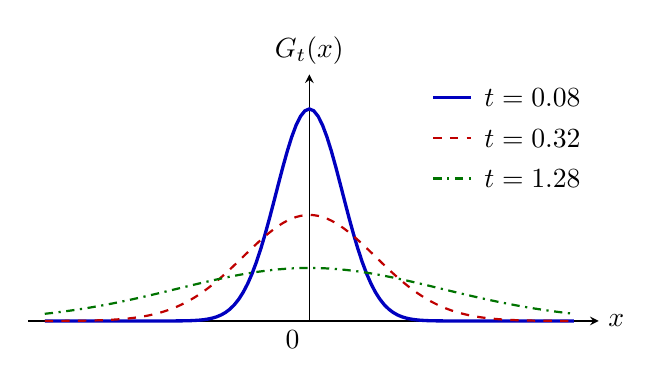
\begin{tikzpicture}[x=1.05cm,y=2.7cm,>=stealth]
	\draw[->] (-3.4,0)--(3.5,0) node[right] {\(x\)};
	\draw[->] (0,0)--(0,1.16) node[above] {\(G_t(x)\)};
	\draw[very thick,blue!75!black,domain=-3.2:3.2,samples=121]
		plot (\x,{exp(-\x*\x/.32)/sqrt(4*pi*.08)});
	\draw[thick,red!75!black,dashed,domain=-3.2:3.2,samples=121]
		plot (\x,{exp(-\x*\x/1.28)/sqrt(4*pi*.32)});
	\draw[thick,green!45!black,dash dot,domain=-3.2:3.2,samples=121]
		plot (\x,{exp(-\x*\x/5.12)/sqrt(4*pi*1.28)});
	\draw[very thick,blue!75!black] (1.5,1.05)--(1.95,1.05);
	\node[right] at (2,1.05) {\(t=0.08\)};
	\draw[thick,red!75!black,dashed] (1.5,.86)--(1.95,.86);
	\node[right] at (2,.86) {\(t=0.32\)};
	\draw[thick,green!45!black,dash dot] (1.5,.67)--(1.95,.67);
	\node[right] at (2,.67) {\(t=1.28\)};
	\node[below left] at (0,0) {\(0\)};
\end{tikzpicture}

	\caption{一维 Euclid Gaussian 核的高度与扩散尺度}
	\label{g3:fig:gaussian-scale}
\end{figure}

\Cref{g3:fig:gaussian-scale}画出三个时刻的一维模型。时间缩小为原来的四分之一时，峰值增大为两倍，集中宽度缩小为一半，而总积分仍为一。流形上将保留这种局部尺度，并用系数修正密度与曲率造成的差别。

\begin{lemma}\label{g3:lem:heat-gaussian-transport-identity}
	设 \((M^n,g)\) 为非空、\(n\ge1\) 维的光滑闭黎曼流形。在 \(d(x,y)<\rho\) 的统一法邻域中，令 \(J\) 和 \(G\) 分别由式\eqref{g3:eq:heat-normal-density}及式\eqref{g3:eq:heat-geodesic-gaussian}定义。取 \(\Delta=-\operatorname{div}\operatorname{grad}\)，定义作用于 \(x\) 变量的算子
	\[
		\mathcal T=r\partial_r+\tfrac12r\partial_r\log J.
	\]
	其中 \(r\partial_r\) 在法坐标中为 \(v^i\partial_{v^i}\)，故在对角上光滑延伸。对任意光滑的 \(a(t,x,y)\)，有
	\begin{equation}\label{g3:eq:heat-gaussian-transport-identity}
		(\partial_t+\Delta_x)(Ga)
		=G\left(\partial_ta+\Delta_xa+t^{-1}\mathcal Ta\right).
	\end{equation}
\end{lemma}
\begin{proof}
	Gauss 引理给出 \(|\mathrm d_xr|=1\)。极坐标中的体积密度为 \(r^{n-1}J_y(r\theta)\,\mathrm dr\,\mathrm d\theta\)，所以在 \(r>0\) 处
	\[
		\Delta r=-\frac{n-1}{r}-\partial_r\log J,
		\qquad \Delta(r^2)=-2n-2r\partial_r\log J.
	\]
	利用 \(\Delta(e^h)=e^h(\Delta h-|\mathrm dh|^2)\)，可得
	\[
		\frac{\partial_tG}{G}=-\frac n{2t}+\frac{r^2}{4t^2},
		\qquad
		\frac{\Delta_xG}{G}=\frac n{2t}
		+\frac{r\partial_r\log J}{2t}-\frac{r^2}{4t^2}.
	\]
	两式的 \(t^{-2}\) 项及常数 \(t^{-1}\) 项抵消。再用
	\(\Delta(Ga)=G\Delta a+a\Delta G-2\langle\mathrm dG,\mathrm da\rangle\)
	和 \(\mathrm dG/G=-r\,\mathrm dr/(2t)\)，便得结论。两边在 \(r=0\) 处均光滑，故等式也在那里成立。
\end{proof}

因而主项的修正首先是一个沿径向测地线的一阶问题。二阶算子 \(\Delta_x\) 将在后一阶才进入递推；这使系数能够逐个确定。

\subsection{运输方程与系数递推}
\label{g3:subsec:1602:02}
寻找形式为 \(G\sum_{j=0}^Nt^ju_j(x,y)\) 的近似解。代入式\eqref{g3:eq:heat-gaussian-transport-identity}，依次令 \(t^{-1},t^0,\ldots,t^{N-1}\) 的系数为零，得到\term[yunshu fangcheng]{运输方程}[transport equation]
\begin{equation}\label{g3:eq:heat-transport-recursion}
	\mathcal Tu_0=0,\qquad
	(\mathcal T+j)u_j=-\Delta_xu_{j-1}\quad(j\ge1),
	\qquad u_0(y,y)=1.
\end{equation}
最后一个条件保证对角上的质量归一化。
\symidx{\(u_j(x,y)\)：短时热核的运输系数}

\begin{proposition}\label{g3:prop:heat-transport-coefficients}
	设 \((M^n,g)\) 为非空、\(n\ge1\) 维的光滑闭黎曼流形，\(\Delta=-\operatorname{div}\operatorname{grad}\)，\(J\) 为式\eqref{g3:eq:heat-normal-density}的法坐标密度。在统一法邻域 \(d(x,y)<\rho\) 上，式\eqref{g3:eq:heat-transport-recursion}有唯一的光滑系数列。具体地，若 \(x=\exp_yv\)、\(z_s=\exp_y(sv)\)，则
	\begin{align}
		u_0(x,y)&=J_y(v)^{-1/2},\label{g3:eq:heat-u0-density}\\
		u_j(x,y)&=-J_y(v)^{-1/2}
		\int_0^1s^{j-1}J_y(sv)^{1/2}
		(\Delta_xu_{j-1})(z_s,y)\,\mathrm ds,
		\quad j\ge1.\label{g3:eq:heat-transport-integral}
	\end{align}
	特别地，
	\begin{equation}\label{g3:eq:heat-diagonal-recursion}
		u_0(y,y)=1,\qquad
		u_j(y,y)=-\frac1j(\Delta_xu_{j-1})(y,y).
	\end{equation}
\end{proposition}
\begin{proof}
	固定 \(y\) 和单位方向 \(\theta\)。把方程乘以 \(r^{j-1}J_y(r\theta)^{1/2}\)，便得到
	\[
		\partial_r\bigl(r^jJ_y(r\theta)^{1/2}u_j(\exp_y(r\theta),y)\bigr)
		=-r^{j-1}J_y(r\theta)^{1/2}
		(\Delta_xu_{j-1})(\exp_y(r\theta),y).
	\]
	当 \(j=0\) 时，右边取零，归一化给出 \(J^{1/2}u_0=1\)。当 \(j\ge1\) 时，光滑性迫使左边括号在 \(r=0\) 为零。从零积分到 \(r\)，再令积分变量为 \(rs\)，即得式\eqref{g3:eq:heat-transport-integral}。

	该积分式也证明了对角处的光滑性。若 \(u_{j-1}\) 联合光滑，其被积函数在 \((s,y,v)\in[0,1]\times\{|v|<\rho\}\) 上光滑，任意固定阶导数可移入有限区间积分，因而 \(u_j\) 联合光滑。由归纳得到全部系数。齐次方程的差解满足 \(r^jJ^{1/2}w\) 沿径向恒定；\(j\ge1\) 时光滑性使该常数为零，\(j=0\) 时由归一化也为零。这证明唯一性。最后令 \(v=0\)，利用 \(\int_0^1s^{j-1}\,\mathrm ds=1/j\)，得到对角公式。
\end{proof}

\begin{example}\label{g3:exm:flat-local-heat-coefficients}
	在一个 Euclid 开片中，\(J=1\)，所以 \(u_0=1\)、\(u_j=0\) 对所有 \(j\ge1\) 成立。同样的结论适用于平坦环面的充分小法邻域。它并不表示环面的全局热核只有一个 Gaussian 项；热流绕过全局闭路所产生的贡献，要由局部核之外的修正记录。
\end{example}

式\eqref{g3:eq:heat-transport-integral}每次只沿唯一短测地线积分，因此系数由该线附近的度量决定。在 \(v=0\) 处对该积分式求固定阶导数，右端只含 \(J\) 及上一系数的有限阶导数；逐层回代到 \(u_0=J^{-1/2}\)，可知对角上的有限阶系数只依赖有限阶度量导数。这里尚未断言无限级数收敛；接下来将对每个有限截断单独给出误差界。

\subsection{截断参数核的误差}
\label{g3:subsec:1602:03}
取 \(\chi\in C^\infty(M\times M)\)，它在 \(r<\rho/3\) 时为一，在 \(r>2\rho/3\) 时为零，且在法邻域中只依赖 \(r^2\)。定义\term[canshu he]{参数核}[parametrix]
\begin{equation}\label{g3:eq:heat-cutoff-parametrix}
	H_N(t,x,y)=\chi(x,y)G(t,x,y)\sum_{j=0}^Nt^ju_j(x,y),
	\qquad R_N=(\partial_t+\Delta_x)H_N,
\end{equation}
并在法邻域外取零。截断使它成为全局光滑核；代价是截断变化的环带上产生附加误差。

\begin{lemma}\label{g3:lem:heat-parametrix-error-bounds}
	设 \((M^n,g)\) 为非空、\(n\ge1\) 维的光滑闭黎曼流形，\(\Delta=-\operatorname{div}\operatorname{grad}\)。固定整数 \(N\ge0\)，按式\eqref{g3:eq:heat-cutoff-parametrix}取参数核 \(H_N\) 及残差 \(R_N\)。在任意固定的有限坐标覆盖及其相对紧小片上，对多重指标 \(\alpha,\beta\) 和整数 \(\ell\ge0\)，存在常数 \(C,c>0\)，使 \(0<t\le1\) 时
	\begin{align}
		|\partial_x^\alpha\partial_y^\beta\partial_t^\ell H_N|
		&\le Ct^{-n/2-(|\alpha|+|\beta|)/2-\ell}e^{-r^2/(ct)},\label{g3:eq:heat-parametrix-gaussian-bound}\\
		|\partial_x^\alpha\partial_y^\beta\partial_t^\ell R_N|
		&\le Ct^{N-n/2-(|\alpha|+|\beta|)/2-\ell}e^{-r^2/(ct)}.\label{g3:eq:heat-residual-gaussian-bound}
	\end{align}
	右端只需在核的支集附近解释；支集外左端为零。对核 \(A\) 记
	\[
		\|A\|_{\mathrm{int}}=
		\max\left\{\sup_x\int_M|A(x,y)|\,\mu_g(y),
		\sup_y\int_M|A(x,y)|\,\mu_g(x)\right\}.
	\]
	则
	\begin{equation}\label{g3:eq:heat-parametrix-integral-bounds}
		\|H_N(t)\|_{\mathrm{int}}\le C,
		\qquad \|R_N(t)\|_{\mathrm{int}}\le Ct^N.
	\end{equation}
	对每个整数 \(m\ge0\)，还成立
	\begin{equation}\label{g3:eq:heat-residual-sobolev-bound}
		\sup_y\|\partial_y^\beta R_N(t,\cdot,y)\|_{H^m(M)}
		\le Ct^{N-n/4-(m+|\beta|)/2}.
	\end{equation}
\end{lemma}
\begin{proof}
	运输方程给出确切公式
	\begin{equation}\label{g3:eq:heat-cutoff-residual}
		R_N=\chi Gt^N\Delta_xu_N
		+(\Delta_x\chi)G\sum_{j=0}^Nt^ju_j
		-2\left\langle\mathrm d_x\chi,
		\mathrm d_x\left(G\sum_{j=0}^Nt^ju_j\right)\right\rangle.
	\end{equation}
	先考察第一项。\(r^2\) 联合光滑，在对角上二阶消失，故其一次导数为 \(O(r)\)，二阶及以上的固定阶导数一致有界。对 \(e^{-r^2/(4t)}\) 求一次空间导数，增加的因子为 \(O(r/t)\)；求高阶导数得到这种因子及 \(O(t^{-1})\) 的有限乘积。把 \(r/\sqrt t\) 的任意固定幂吸收到略弱的 Gaussian 中，即
	\[
		s^a e^{-s^2/4}\le C_a e^{-s^2/8}\quad(s\ge0),
	\]
	便知每一空间导数至多损失 \(t^{-1/2}\)。一次时间导数至多损失 \(t^{-1}\)。系数及其固定阶导数在截断支集上一致有界，因此得到所需估计。

	式\eqref{g3:eq:heat-cutoff-residual}的后两项支集满足 \(r\ge\rho/3\)。在那里，对于任意 \(A,B>0\)，均有 \(t^{-A}e^{-\rho^2/(Bt)}=O(t^L)\)，其中 \(L\) 可任意指定。这由令 \(s=1/t\) 后指数压过多项式直接得到。留出一部分 Gaussian 衰减，便能吸收截断项产生的全部负幂并补足 \(t^N\)。同一计算给出 \(H_N\) 的导数估计。

	法坐标中的 \(J\) 在所用紧集上有一致上下界，故缩放 \(v=\sqrt t\,w\) 给出
	\[
		\sup_y\int_{r<\rho}e^{-r^2/(ct)}\,\mu_g(x)\le C_ct^{n/2},
	\]
	交换 \(x,y\) 后同样成立。积分点态界便得式\eqref{g3:eq:heat-parametrix-integral-bounds}。将残差的空间导数界平方后积分、开平方，得到 \(L^2\) 因子 \(t^{n/4}\)；再把 \(x\) 变量中不超过 \(m\) 阶的导数相加，便得式\eqref{g3:eq:heat-residual-sobolev-bound}。有限覆盖及光滑截断只改变常数。
\end{proof}

\begin{lemma}\label{g3:lem:heat-parametrix-initial-value}
	设 \((M^n,g)\) 为非空、\(n\ge1\) 维的光滑闭黎曼流形。对任意整数 \(N\ge0\)，式\eqref{g3:eq:heat-cutoff-parametrix}的核 \(H_N(t)\) 在 \(0<t\le1\) 时定义 \(L^2(M)\) 上一致有界的算子。若 \(f\in C^0(M)\)，则 \(t\downarrow0\) 时 \(H_N(t)f\to f\) 一致；若 \(f\in L^2(M)\)，则此收敛在 \(L^2\) 中成立。
\end{lemma}
\begin{proof}
	对任意核 \(A\)，两次使用积分估计得到
	\[
		|Af(x)|^2\le
		\left(\int|A(x,y)|\,\mu_g(y)\right)
		\left(\int|A(x,y)||f(y)|^2\,\mu_g(y)\right),
		\quad \|Af\|_2\le\|A\|_{\mathrm{int}}\|f\|_2.
	\]
	因此上一引理给出算子的一致有界性。

	对连续 \(f\)，在以 \(x\) 为中心的法坐标 \(y=\exp_xw\) 中作 \(w=\sqrt t\,z\)。被积的光滑系数在 \(w=0\) 的值为 \(u_0(x,x)J_x(0)=1\)。在任意固定的小球内，它与 \(f(y)\) 相乘后一致接近 \(f(x)\)；小球外的 Gaussian 积分一致趋零。Euclid Gaussian 总质量为一，所以零阶项趋于 \(f(x)\)，且由紧性收敛一致。其余项含 \(t^j\)、\(j\ge1\)，积分范数为 \(O(t^j)\)，因而趋零。最后用光滑函数在 \(L^2\) 中的稠密性及已证的一致算子界，得到一般初值的强收敛。
\end{proof}

\subsection{Volterra 修正及余项控制}
\label{g3:subsec:1602:04}
对于两个随时间变化的核，定义只积分过去时间的卷积
\begin{equation}\label{g3:eq:heat-volterra-convolution}
	(A*B)(t,x,y)=\int_0^t\int_M
	A(t-s,x,z)B(s,z,y)\,\mu_g(z)\,\mathrm ds.
\end{equation}
这样的积分称为 \term[Volterra juanji]{Volterra 卷积}[Volterra convolution]。\footnote{Samuel Giuseppe Vito Volterra（1860--1940），意大利数学家，研究积分方程、泛函分析及数学物理；其积分方程方法将逐次代入与连续变量中的极限联系起来。}在以下绝对收敛的范围内，Fubini 定理给出结合律。若 \(R_N\) 是 \(H_N\) 的误差，就希望找 \(\Phi_N\) 满足
\[
	\Phi_N+R_N+R_N*\Phi_N=0.
\]
逐次代入给出候选级数 \(-R_N+R_N*R_N-\cdots\)。其收敛来自时间单纯形的阶乘，而不要求 \(R_N(t)\) 在每个时刻的算子范数都小于一。

\begin{lemma}\label{g3:lem:heat-volterra-series}
	设 \((M^n,g)\) 为非空、\(n\ge1\) 维的光滑闭黎曼流形。固定整数 \(N>n/2\)，令 \(R=R_N\) 为式\eqref{g3:eq:heat-cutoff-parametrix}中非负标量 Laplace 算子的残差，按式\eqref{g3:eq:heat-volterra-convolution}定义 \(R^{*1}=R\)、\(R^{*(k+1)}=R*R^{*k}\)。对 \(0<t\le1\)，有
	\begin{align}
		\|R^{*k}(t)\|_{\mathrm{int}}
		&\le\frac{C^k(N!)^k}{(k(N+1)-1)!}
		t^{k(N+1)-1},\label{g3:eq:heat-volterra-integral-power}\\
		\|R^{*k}(t)\|_\infty
		&\le\frac{k^{n/2}C^k(N!)^k}{(k(N+1)-1)!}
		t^{k(N+1)-1-n/2}.\label{g3:eq:heat-volterra-point-power}
	\end{align}
	因此
	\begin{equation}\label{g3:eq:heat-volterra-correction}
		\Phi_N=\sum_{k=1}^\infty(-1)^kR_N^{*k}
	\end{equation}
	在 \([0,1]\times M\times M\) 上一致收敛为连续核，在 \(t=0\) 取零，并且
	\begin{equation}\label{g3:eq:heat-volterra-correction-bounds}
		\Phi_N+R_N+R_N*\Phi_N=0,
		\quad \|\Phi_N(t)\|_{\mathrm{int}}\le Ct^N,
		\quad \|\Phi_N(t)\|_\infty\le Ct^{N-n/2}.
	\end{equation}
\end{lemma}
\begin{proof}
	把 \(k\) 重卷积写成时间单纯形 \(\tau_i>0\)、\(\sum_i\tau_i=t\) 上的积分。对每个固定时间组，空间核复合的积分范数不超过各因子积分范数之积，因此不超过 \(C^k\prod_i\tau_i^N\)。反复使用
	\[
		\int_0^t(t-s)^as^b\,\mathrm ds
		=\frac{a!b!}{(a+b+1)!}t^{a+b+1}
		\quad(a,b\text{ 为非负整数})
	\]
	便得式\eqref{g3:eq:heat-volterra-integral-power}；这个一维公式可由分部积分对 \(a\) 归纳证明。

	为估计点态值，在每个时间组中选最大的 \(\tau_j\)，于是 \(\tau_j\ge t/k\)。将第 \(j\) 个核用点态界 \(C\tau_j^{N-n/2}\) 控制，其前面的核依次用行积分界，后面的核依次用列积分界，所得空间积分至多为
	\[
		C^k\tau_j^{-n/2}\prod_i\tau_i^N
		\le C^k(k/t)^{n/2}\prod_i\tau_i^N.
	\]
	再积分同一个时间单纯形即得第二个估计。这一步同时用到了行、列两种积分界。

	阶乘分母使两个级数在 \(0<t\le1\) 上绝对收敛；提取首项的 \(t^N\) 或 \(t^{N-n/2}\) 后，余下级数仍一致有界。\(R_N\) 因 \(N>n/2\) 连续延伸为零，有限重卷积也连续；上述一致收敛遂给出 \(\Phi_N\) 的连续性。利用积分界交换求和与卷积，相邻各项抵消，得到第一条恒等式。
\end{proof}

\begin{proposition}\label{g3:prop:heat-local-corrected-kernel}
	设 \((M^n,g)\) 为非空、\(n\ge1\) 维的光滑闭黎曼流形，\(\Delta=-\operatorname{div}\operatorname{grad}\)。对任意整数 \(N>n/2\)，取式\eqref{g3:eq:heat-cutoff-parametrix}的参数核 \(H_N\) 及式\eqref{g3:eq:heat-volterra-correction}的核 \(\Phi_N\)，令
	\begin{equation}\label{g3:eq:heat-local-corrected-kernel}
		\widetilde K_N=H_N+H_N*\Phi_N.
	\end{equation}
	它在 \((0,1]\times M\times M\) 上连续，满足分布方程
	\((\partial_t+\Delta_x)\widetilde K_N=0\)，并且
	\begin{equation}\label{g3:eq:heat-volterra-remainder}
		\|\widetilde K_N(t)-H_N(t)\|_\infty
		\le Ct^{N+1-n/2},\qquad
		\|\widetilde K_N(t)-H_N(t)\|_{\mathrm{int}}
		\le Ct^{N+1}.
	\end{equation}
	对任意 \(f\in L^2(M)\)，\(\widetilde K_N(t)f\) 连续延伸到 \(t=0\)，其 \(L^2\) 初值为 \(f\)。
\end{proposition}
\begin{proof}
	积分范数估计直接来自
	\(\int_0^t\|H_N(t-s)\|_{\mathrm{int}}
	\|\Phi_N(s)\|_{\mathrm{int}}\,\mathrm ds\le Ct^{N+1}\)。
	点态估计把积分分成 \(s\le t/2\) 和 \(s\ge t/2\)。在第一段，用 \(H_N(t-s)\) 的上确界和 \(\Phi_N(s)\) 的列积分界；在第二段，用 \(H_N(t-s)\) 的行积分界和 \(\Phi_N(s)\) 的上确界。于是
	\[
		|H_N*\Phi_N|
		\le C\int_0^{t/2}(t-s)^{-n/2}s^N\,\mathrm ds
		+C\int_{t/2}^ts^{N-n/2}\,\mathrm ds
		\le Ct^{N+1-n/2}.
	\]
	在固定的正时间附近，避开两个积分端点后被积核连续且有界；接近 \(s=0\) 的部分由上述界控制，接近 \(s=t\) 的长度为 \(\varepsilon\) 的部分由 \(H_N\) 的行积分界控制为 \(C\varepsilon\)。先截去端点，再让 \(\varepsilon\downarrow0\)，证明卷积连续。相同论证与积分范数界也给出作用于 \(L^2\) 后的正时间连续性，初值则由\cref{g3:lem:heat-parametrix-initial-value}得到。

	为了验证方程，将 \(H_N,R_N\) 在负时间延为零。对任意光滑紧支集的双变量时空测试函数 \(\psi(t,x,y)\)，沿法坐标作与初值引理相同的缩放，可得
	\[
		\int_{M\times M}H_N(\varepsilon,x,y)\psi(\varepsilon,x,y)
		\,\mu_g(x)\mu_g(y)
		\longrightarrow\int_M\psi(0,x,x)\,\mu_g(x).
	\]
	具体说，在对角附近令 \(y=\exp_x(\sqrt\varepsilon\,v)\)，光滑系数一致趋于 \(\psi(0,x,x)\)，外部尾项由 Gaussian 控制；高阶项含正幂 \(\varepsilon^j\)，因而消失。于是以 \(\psi\) 配对，在 \(t\ge\varepsilon\) 上对时间分部积分，再令 \(\varepsilon\downarrow0\)，得到
	\[
		(\partial_t+\Delta_x)H_N
		=\delta_0(t)I+R_N
	\]
	的核分布恒等式。这里 \(I\) 的核是对角上的单位分布；残差在零附近可积，所以取极限合法。再与 \(\Phi_N\) 卷积，Fubini 定理和前述绝对积分界给出
	\[
		(\partial_t+\Delta_x)(H_N*\Phi_N)
		=\Phi_N+R_N*\Phi_N.
	\]
	这也可先让测试函数避开时间端点，再按同样估计取极限。因此 \(t>0\) 时，\(\widetilde K_N\) 的残差为 \(R_N+\Phi_N+R_N*\Phi_N=0\)。整个计算在分布意义下进行，未对零时间处奇异的 Gaussian 核直接求导后交换积分。
\end{proof}

\subsection{局部构造与谱核的一致性}
\label{g3:subsec:1602:05}
现在已有一个满足正确方程和初值的连续核。对 \(f\in L^2(M)\)，\cref{g3:thm:heat-spectral-solution}的唯一性立即给出
\[
	\widetilde K_N(t)f=T_tf\qquad(0<t\le1).
\]
两侧的连续积分核必相同：固定 \(x\) 后，核之差与所有 \(L^2\) 函数积分为零，取该行之差的复共轭作测试即可。因此 \(\widetilde K_N=K\)，其中 \(K\) 是上一节的谱核。这同时证明了它不依赖所选截断函数或足够大的 \(N\)，并且在正时间联合光滑。

\ProseParagraphBreak

下一定理给出全部有限阶导数的误差。其证明先取比目标阶数更高的截断，得到一个很小的光滑误差，然后把多取的有限项减回去。这样可以分别控制零时间的可积性和最终余项的精确阶数。

\begin{theorem}\label{g3:thm:heat-parametrix-expansion}
	设 \((M^n,g)\) 为非空、\(n\ge1\) 维的光滑闭黎曼流形，\(K\) 是非负算子 \(\Delta=-\operatorname{div}\operatorname{grad}\) 的热核。取上述法邻域、截断函数及运输系数。对每个整数 \(N\ge0\)，有
	\begin{equation}\label{g3:eq:heat-parametrix-expansion}
		K(t,x,y)=\chi(x,y)(4\pi t)^{-n/2}e^{-r^2/(4t)}
		\sum_{j=0}^Nt^ju_j(x,y)+E_N(t,x,y).
	\end{equation}
	对任意固定的多重指标 \(\alpha,\beta\) 和整数 \(\ell\ge0\)，在有限坐标覆盖的相对紧小片上存在一致常数，使
	\begin{equation}\label{g3:eq:heat-parametrix-derivative-remainder}
		|\partial_x^\alpha\partial_y^\beta\partial_t^\ell E_N(t,x,y)|
		\le Ct^{N+1-n/2-(|\alpha|+|\beta|)/2-\ell},
		\qquad 0<t\le1.
	\end{equation}
	特别地，以下对角余项对 \(x\in M\) 一致：
	\begin{equation}\label{g3:eq:heat-diagonal-uniform-remainder}
		K(t,x,x)=(4\pi t)^{-n/2}\sum_{j=0}^Nt^ju_j(x,x)
		+O(t^{N+1-n/2}).
	\end{equation}
\end{theorem}
\begin{proof}
	先说明高阶残差如何控制误差。由\cref{g3:thm:elliptic-spectral-sobolev}，对每个偶数 \(m=2q\)，算子 \(T_t\) 在 \(H^m\) 上一致有界，\(0\le t\le1\)：在等价的谱范数中，它只把各系数乘以 \(e^{-t\lambda_j}\le1\)。

	若整数 \(L\) 足够大，使式\eqref{g3:eq:heat-residual-sobolev-bound}的右端在零附近可积，则令
	\begin{equation}\label{g3:eq:heat-high-remainder-duhamel}
		W_L(t,\cdot,y)=-\int_0^tT_{t-s}R_L(s,\cdot,y)\,\mathrm ds.
	\end{equation}
	这是 \(H^m\) 中的积分，且初值为零。为核对方程，将被积函数投到特征函数 \(\phi_j\) 上，所得系数为
	\[
		-\int_0^te^{-(t-s)\lambda_j}
		(R_L(s,\cdot,y),\phi_j)\,\mathrm ds.
	\]
	该系数满足导数加 \(\lambda_j\) 倍自身等于残差系数的负值。有限谱和满足非齐次方程，利用 \(L^1((0,1);H^m)\) 的残差控制，取极限即得 \((\partial_t+\Delta)W_L=-R_L\) 的分布等式。

	取 \(L>n/2\)。已经证明的式\eqref{g3:eq:heat-volterra-remainder}说明 \(E_L=K-H_L\) 对每个固定 \(y\) 在 \(t=0\) 有零 \(L^2\) 初值；它满足同一非齐次方程。因此 \(E_L-W_L\) 是零初值的 \(L^2\) 连续齐次分布解，唯一性给出 \(E_L=W_L\)。对 \(y\) 求固定阶导数也可以移入式\eqref{g3:eq:heat-high-remainder-duhamel}，因为相应的 \(H^m\) 范数有统一可积上界。于是
	\begin{equation}\label{g3:eq:heat-high-remainder-sobolev}
		\sup_y\|\partial_y^\beta E_L(t,\cdot,y)\|_{H^m}
		\le Ct^{L+1-n/4-(m+|\beta|)/2}.
	\end{equation}

	现在固定 \(N,\alpha,\beta,\ell\)。选择偶数 \(m>|\alpha|+2\ell+n/2\)，再选择整数
	\[
		L\ge N+m+|\beta|+2\ell+n+2.
	\]
	这些选择保证以上积分可积，也保证式\eqref{g3:eq:heat-high-remainder-sobolev}的指数不小于目标指数
	\(N+1-n/2-(|\alpha|+|\beta|)/2-\ell\)。由高阶 Sobolev 嵌入，它控制 \(E_L\) 的 \(x\) 变量中不超过 \(|\alpha|+2\ell\) 阶的导数。时间导数用已经成立的方程递推：
	\[
		\partial_t^\ell E_L=(-\Delta)^\ell E_L
		-\sum_{j=0}^{\ell-1}(-\Delta)^{\ell-1-j}\partial_t^jR_L
		\qquad(\ell\ge1).
	\]
	第一项由刚才的 Sobolev 界控制。对求和项使用式\eqref{g3:eq:heat-residual-gaussian-bound}，其空间阶数为 \(|\alpha|+2(\ell-1-j)\)，时间阶数为 \(j\)，故指数至少为
	\(L+1-n/2-(|\alpha|+|\beta|)/2-\ell\)，也足够。这里全在正时间的光滑函数上运算。

	最后写
	\[
		E_N=E_L+(H_L-H_N)
		=E_L+\chi G\sum_{j=N+1}^Lt^ju_j.
	\]
	有限和的每项经同样的 Gaussian 导数估计，恰好满足式\eqref{g3:eq:heat-parametrix-derivative-remainder}。合并两部分即得结论。对角上 \(\chi=1\)、\(r=0\)，令 \(\alpha=\beta=\ell=0\) 得最后一式。
\end{proof}

这一展开是逐个 \(N\) 的渐近断言，不需要 \(\sum_{j\ge0}t^ju_j\) 收敛。离开对角的任意固定邻域，显式 Gaussian 项连同所有固定阶导数均小于任意幂；再任意提高 \(N\)，可知真正热核在该区域也具有同样的任意幂衰减。对角系数则保存了短时仍然可见的几何信息。

\ProseParagraphBreak

后续的 Hodge 与 Dirac 问题需要丛值版本。下面把新增的几何步骤写出；时间卷积与余项估计仍是已经证明的有限维范数估计。

\begin{proposition}\label{g3:prop:laplace-type-heat-parametrix}
	设 \((M^n,g)\) 为非空、\(n\ge1\) 维的光滑闭黎曼流形，\(E\to M\) 为正秩光滑 Hermitian 丛，\(\nabla\) 为相容联络，\(V\) 为光滑自伴丛自同态。假设 \(P=\nabla^*\nabla+V\) 非负。令 \(\tau(x,y):E_y\to E_x\) 为沿唯一短径向测地线的平行移动，则 \(P\) 的热核有式\eqref{g3:eq:heat-parametrix-expansion}及式\eqref{g3:eq:heat-parametrix-derivative-remainder}的丛值版本，其中乘积解释为纤维映射复合，导数在有限光滑平凡化中计算。其系数满足
	\begin{align}
		u_0^E(x,y)&=J(x,y)^{-1/2}\tau(x,y),\label{g3:eq:bundle-heat-leading-coefficient}\\
		\left(r\nabla_{\partial_r}+\tfrac r2\partial_r\log J+j\right)u_j^E
		&=-P_xu_{j-1}^E\qquad(j\ge1),\label{g3:eq:bundle-heat-transport}\\
		u_1^E(y,y)&=u_1(y,y)I_{E_y}-V(y).\label{g3:eq:bundle-heat-first-potential}
	\end{align}
	这里 \(u_1\) 是同一度量的标量系数。
\end{proposition}
\begin{proof}
	对标量 \(G\) 与丛值 \(a\)，相容联络的乘法公式为
	\[
		P(Ga)=GPa+(\Delta G)a-2\nabla_{\operatorname{grad}G}a.
	\]
	所以 Gaussian 计算只需把径向普通导数换为协变导数。由于 \(\nabla_{\partial_r}\tau=0\)，零阶运输方程给出所述 \(u_0^E\)。令 \(x=\exp_yv\)、\(z_s=\exp_y(sv)\)，高阶解具体为
	\[
		u_j^E(x,y)=-J(x,y)^{-1/2}\tau(x,y)
		\int_0^1s^{j-1}J(z_s,y)^{1/2}\tau(z_s,y)^{-1}
		(P_xu_{j-1}^E)(z_s,y)\,\mathrm ds.
	\]
	平行移动对端点光滑依赖，所以此式给出联合光滑的系数；径向常微分方程和对角正则性再次给出唯一性。固定有限平凡化，矩阵的算子范数满足 \(\|AB\|\le\|A\|\|B\|\)，且纤维秩有限。因此残差估计、行列积分界、时间单纯形估计与收敛级数逐项成立。上一节的丛值谱核具有同一 \(L^2\) 连续分布解唯一性；第十三章的丛值谱范数又给出 \(H^{2q}\) 上的一致有界性。因此识别及高阶余项证明的每一步均适用。

	最后核算 \(u_1^E\)。固定 \(y\)，从 \(E_y\) 的正交标架作径向平行移动。在所得标架中，\(\tau\) 的矩阵为常值 \(I\)，联络矩阵 \(A_i(v)\) 满足 \(v^iA_i(v)=0\)。一次微分后在 \(v=0\) 取值，得 \(A_i(0)=0\)；二次微分给出 \(\partial_iA_j(0)+\partial_jA_i(0)=0\)，特别有 \(\sum_i\partial_iA_i(0)=0\)。法坐标在中心的 Christoffel 符号也为零，故 \((\nabla^*\nabla\tau)(y,y)=0\)。又因 \(\mathrm d_xJ(y,y)=0\)，乘法公式给出
	\[
		(P_xu_0^E)(y,y)=(\Delta_xJ^{-1/2})(y,y)I+V(y).
	\]
	在一阶运输方程的对角上取值，再与标量公式\eqref{g3:eq:heat-diagonal-recursion}比较，即得式\eqref{g3:eq:bundle-heat-first-potential}。
\end{proof}

下一节的\cref{g3:prop:heat-diagonal-first-coefficients}将由法坐标体积密度算出 \(u_1(x,x)=\operatorname{Scal}(x)/6\)。因此丛值一阶系数为 \(\operatorname{Scal}(x)I/6-V(x)\)：度量的体积扩张与算子的零阶势分别贡献这两个项。
% 纲要条目排为编号小节标题，并进入目录与书签；说明段仍保留于纲要注释中。

% !TeX root = ../../Book3.tex
% 纲要标题：### 16.3 热迹和谱渐近
% 纲要位置：几何学计划纲要.md，第 2766 行。
% 正文状态：初稿；尚未正式审核。

% 纲要内容开始
% 
% * 对角系数与体积、标量曲率
% * 积分余项与热迹展开
% * 正测度的 Tauber 引理
% * Weyl 律与特征值增长
% 
% 纲要内容结束

\section{热迹和谱渐近}
\label{g3:sec:1603}

短时间内，热核主要集中在距离约为 \(\sqrt t\) 的邻域。上一节把这种集中写成 Gaussian 因子与光滑系数的乘积；现在沿对角积分，就能把局部度量信息转成全体特征值的共同约束。体积决定热迹的首项，标量曲率的积分决定下一项。要进一步知道某个阈值以下有多少特征值，还须从指数加权的和中恢复没有平滑的计数函数。

\ProseParagraphBreak

本节设 \((M,g)\) 是非空的 \(n\) 维光滑闭黎曼流形，\(n\ge1\)，不要求连通或定向。沿用 \(\Delta=-\operatorname{div}\nabla\)、黎曼体积密度 \(\mu_g\)，以及式\eqref{g3:eq:heat-spectrum-enumeration}中从 \(j=0\) 开始、按重数排列且包含全部零模的特征值 \(\lambda_j\)。局部系数仍记为 \(u_j(x,y)\)，其中 Laplace 算子作用于第一个变量。

\subsection{对角系数与体积、标量曲率}
\label{g3:subsec:1603:01}
固定 \(y\in M\)，在以 \(y\) 为中心的正交法坐标中写
\[
	x=\exp_y(v),\qquad r=|v|,\qquad
	\exp_y^*\mu_g=J_y(v)\,\mathrm dv.
\]
这里 \(J_y(0)=1\)。体积密度 \(J_y\) 描述指数映射对体积的改变，而热核的主振幅正好补偿其中一半的改变。

\begin{proposition}\label{g3:prop:heat-diagonal-first-coefficients}
	设 \((M,g)\) 是非空的 \(n\ge1\) 维光滑闭黎曼流形，\(\Delta=-\operatorname{div}\nabla\)，\(u_j(x,y)\) 是由上一节运输方程构造的标量热核局部系数。在对角的充分小邻域内，首系数为
	\begin{equation}\label{g3:eq:heat-leading-density}
		u_0(\exp_y(v),y)=J_y(v)^{-1/2}.
	\end{equation}
	前两个对角系数满足
	\begin{equation}\label{g3:eq:heat-first-diagonal-values}
		u_0(y,y)=1,\qquad
		u_1(y,y)=\frac16\operatorname{Scal}_g(y).
	\end{equation}
\end{proposition}
\begin{proof}
	上一节的运输方程为
	\[
		\left(r\partial_r+\frac r2\partial_r\log J_y\right)u_0=0,
		\qquad u_0(y,y)=1,
	\]
	以及对 \(j\ge1\)，
	\[
		\left(r\partial_r+j+\frac r2\partial_r\log J_y\right)u_j
		=-\Delta_xu_{j-1}.
	\]
	在每条径向测地线上，第一个方程等价于
	\(\partial_r(J_y^{1/2}u_0)=0\)。用 \(r=0\) 时的值确定常数，得到式\eqref{g3:eq:heat-leading-density}。

	由\cref{g3:prop:normal-volume-density}的法坐标展开，
	\[
		J_y(v)=1-\frac16\operatorname{Ric}_{ab}(y)v^av^b+O(|v|^3),
	\]
	所以
	\[
		u_0(\exp_y(v),y)
		=1+\frac1{12}\operatorname{Ric}_{ab}(y)v^av^b+O(|v|^3).
	\]
	这些是光滑函数的 Taylor 展开；余项的二阶导数在原点为零，因此二阶导数由显示出的二次项确定。在法坐标中心 \(g_{ab}=\delta_{ab}\)、\(\partial_cg_{ab}=0\)，故
	\[
		\left.\Delta_xu_0(x,y)\right|_{x=y}
		=-\left.\sum_a\partial_{v^a}^2
		\left(1+\frac1{12}\operatorname{Ric}_{bc}(y)v^bv^c\right)
		\right|_{v=0}
		=-\frac16\sum_a\operatorname{Ric}_{aa}(y).
	\]
	最后在 \(j=1\) 的运输方程中令 \(v=0\)。径向向量场
	\(r\partial_r=\sum_av^a\partial_{v^a}\) 在原点消失，且
	\(r\partial_r\log J_y\) 也在那里为零，得到
	\(u_1(y,y)=-\Delta_xu_0(y,y)=\operatorname{Scal}_g(y)/6\)。
\end{proof}

这一计算同时检查了符号与常数：正标量曲率使 \(u_1(x,x)\) 为正。其来源是法坐标体积密度中的负二次项，经负半次幂变号，再经非负号约定的 Laplace 算子变号，最后运输方程右侧还带一个负号。局部递推与对角系数的标准处理可参见 \cite[第2章，2.5--2.6节]{BerlineGetzlerVergne2004}。

\begin{example}\label{g3:exm:constant-curvature-heat-coefficient}
	若度量的截面曲率恒为 \(\kappa\)，则
	\(\operatorname{Ric}=(n-1)\kappa g\)，从而
	\(u_1(x,x)=n(n-1)\kappa/6\)。半径为 \(R\) 的圆球面上这个值为 \(n(n-1)/(6R^2)\)。平坦度量则有更强的局部结论：在充分小的平坦坐标中 \(J_y=1\)，故 \(u_0=1\)；由运输方程及其光滑解的唯一性，逐次得到 \(u_j=0\)（\(j\ge1\)）。这说明平坦闭流形上所有更高的局部幂次系数均为零，尽管热核仍受到全局几何的影响。
\end{example}

\subsection{积分余项与热迹展开}
\label{g3:subsec:1603:02}
由\cref{g3:prop:heat-kernel-trace}，\term[reji]{热迹}[heat trace]有两个相等的表达式：
\[
	Z(t)=\operatorname{Tr}(e^{-t\Delta})
	=\sum_{j=0}^{\infty}e^{-t\lambda_j}
	=\int_M K(t,x,x)\,\mu_g(x).
\]
谱表达式只含特征值；积分表达式允许使用局部构造。连接两者时，关键是上一节的余项对整个对角一致。

\begin{theorem}\label{g3:thm:heat-trace-expansion}
	设 \((M,g)\) 为非空的 \(n\ge1\) 维光滑闭黎曼流形。定义
	\[
		a_\ell(g)=\int_Mu_\ell(x,x)\,\mu_g(x),\qquad \ell=0,1,\ldots.
	\]
	对每个整数 \(N\ge0\)，当 \(t\downarrow0\) 时有
	\begin{equation}\label{g3:eq:heat-trace-full-expansion}
		Z(t)=(4\pi t)^{-n/2}
		\left(\sum_{\ell=0}^{N}a_\ell(g)t^\ell+O(t^{N+1})\right).
	\end{equation}
	其中
	\begin{equation}\label{g3:eq:heat-trace-first-two}
		a_0(g)=\operatorname{Vol}_g(M),\qquad
		a_1(g)=\frac16\int_M\operatorname{Scal}_g\,\mu_g.
	\end{equation}
\end{theorem}
\begin{proof}
	\Cref{g3:thm:heat-parametrix-expansion}的截断函数在对角附近恒为一，Gaussian 因子在 \(x=y\) 时也为一。因此存在 \(C_N,t_N>0\)，使对所有 \(x\in M\) 和 \(0<t\le t_N\)，
	\[
		\left|K(t,x,x)-(4\pi t)^{-n/2}
		\sum_{\ell=0}^{N}t^\ell u_\ell(x,x)\right|
		\le C_Nt^{N+1-n/2}.
	\]
	在 \(M\) 上积分，误差的绝对值不超过
	\(C_N\operatorname{Vol}_g(M)t^{N+1-n/2}\)。
	再用热核迹公式，即得式\eqref{g3:eq:heat-trace-full-expansion}。前两个系数由\cref{g3:prop:heat-diagonal-first-coefficients}直接积分得到。
\end{proof}

式\eqref{g3:eq:heat-trace-full-expansion}是一项一项提高精度的渐近展开。它表示每次固定 \(N\) 后都有相应的误差估计，并不要求无穷级数 \(\sum_\ell a_\ell t^\ell\) 收敛。若 \(M\) 有多个连通分支，热迹及每个 \(a_\ell\) 都按分支相加。

\ProseParagraphBreak

全展开使用包含零特征值的热迹 \(Z(t)\)。设零特征值重数为 \(m_0\)，则仅对正特征值求和得到 \(Z(t)-m_0\)。这个有界差不影响 \(t^{-n/2}\) 的首项，却不能在讨论完整展开时省略；当 \(n\) 为偶数时，它正好改变常数次幂的系数。

\ProseParagraphBreak

为了从热迹读出计数，定义正离散测度和\term[pujishu hanshu]{谱计数函数}[spectral counting function]
\begin{equation}\label{g3:eq:spectral-counting-measure}
	\nu=\sum_{j=0}^{\infty}\delta_{\lambda_j},\qquad
	N(\Lambda)=\nu([0,\Lambda])
	=\#\{j\ge0:\lambda_j\le\Lambda\},\qquad \Lambda\ge0.
\end{equation}
每个特征值的重数由重复的点质量体现；在每个有界区间内只有有限个这样的点质量。于是
\[
	Z(t)=\int_{[0,\infty)}e^{-t\lambda}\,\mathrm d\nu(\lambda).
\]
指数权把不连续的阶梯函数平滑为 \(Z(t)\)。下面证明，正性足以把热迹的首项转换成计数函数的首项。
\symidx{\(N(\Lambda)\)：包含零模并按重数计算的谱计数函数}

\subsection{正测度的 Tauber 引理}
\label{g3:subsec:1603:03}
从变换的渐近行为恢复原对象的渐近行为，称为 Tauber 型问题。\footnote{Alfred Tauber（1866--1942），长期在维也纳任教的数学家，研究分析学、级数与函数论。}下面的\term[Tauber yinli]{Tauber 引理}[Tauberian lemma]只要求测度非负，适用于刚才的离散谱测度。证明中将正半轴缩放后变成紧区间，再用多项式逼近恢复一个区间的质量；所需逼近也在证明中给出。

\begin{lemma}\label{g3:lem:laplace-tauber-counting}
	设 \(\nu\) 是 \([0,\infty)\) 上的非负局部有限 Borel 测度，并且
	\[
		F(t)=\int_{[0,\infty)}e^{-t\lambda}\,\mathrm d\nu(\lambda)<\infty
		\qquad(t>0).
	\]
	若存在 \(A>0,\alpha>0\)，使 \(t^\alpha F(t)\to A\)（\(t\downarrow0\)），则
	\begin{equation}\label{g3:eq:laplace-tauber-limit}
		\lim_{R\to\infty}R^{-\alpha}\nu([0,R])
		=\frac{A}{\Gamma(\alpha+1)}.
	\end{equation}
	这里
	\(\Gamma(s)=\int_0^\infty e^{-x}x^{s-1}\,\mathrm dx\)（\(s>0\)）。
\end{lemma}
\begin{proof}
	先说明极限测度应是什么。定义缩放测度
	\[
		\nu_R(B)=R^{-\alpha}\nu(RB)
		\quad(B\subset[0,\infty)\text{ 为 Borel 集}).
	\]
	对每个固定 \(s>0\)，有
	\begin{equation}\label{g3:eq:tauber-scaled-laplace}
		\int e^{-sx}\,\mathrm d\nu_R(x)
		=R^{-\alpha}F(s/R)\longrightarrow As^{-\alpha}.
	\end{equation}
	而密度测度
	\[
		\mathrm d\nu_\infty(x)
		=\frac{A}{\Gamma(\alpha)}x^{\alpha-1}\,\mathrm dx
	\]
	具有同一 Laplace 变换 \(As^{-\alpha}\)：在积分中作代换 \(z=sx\) 即得。Gamma 积分在零点因 \(\alpha>0\) 可积，在无穷远因指数衰减可积。分部积分还给出
	\(\Gamma(\alpha+1)=\alpha\Gamma(\alpha)\)。

	这些测度在整个正半轴上的总质量可能无穷，所以先乘一个指数权。对 \(f\in C([0,1])\)，用
	\begin{equation}\label{g3:eq:tauber-compact-measures}
		\int_{[0,1]}f(y)\,\mathrm d\rho_R(y)
		=\int_{[0,\infty)}f(e^{-x})e^{-x}\,\mathrm d\nu_R(x)
	\end{equation}
	定义有限正测度 \(\rho_R\)；这是测度 \(e^{-x}\mathrm d\nu_R\) 在映射 \(x\mapsto e^{-x}\) 下的推前，在 \(y=0\) 处赋质量零。用 \(\nu_\infty\) 同样定义 \(\rho_\infty\)。式\eqref{g3:eq:tauber-scaled-laplace}说明，对每个整数 \(k\ge0\)，
	\[
		\int y^k\,\mathrm d\rho_R
		\longrightarrow A(k+1)^{-\alpha}
		=\int y^k\,\mathrm d\rho_\infty.
	\]
	尤其 \(\rho_R([0,1])\to A\)，这些总质量在 \(R\) 充分大时一致有界。有限线性组合立即给出任意多项式的积分收敛。

	现在把多项式换成连续函数。对实连续函数 \(f\)，令
	\[
		P_mf(y)=\sum_{k=0}^{m}f(k/m)\binom{m}{k}y^k(1-y)^{m-k}.
	\]
	权 \(p_{m,k}(y)=\binom{m}{k}y^k(1-y)^{m-k}\) 非负，和为一。由二项式恒等式及其一、二阶导数，
	\[
		\sum_k(k/m)p_{m,k}=y,\qquad
		\sum_k(k/m-y)^2p_{m,k}
		=\frac{y(1-y)}m\le\frac1{4m}.
	\]
	设 \(\omega_f(\delta)=\sup_{|z-y|\le\delta}|f(z)-f(y)|\)。把和分成
	\(|k/m-y|\le\delta\) 与其补集，第二部分的权之和不超过
	\(1/(4m\delta^2)\)，于是
	\[
		\lVert P_mf-f\rVert_\infty
		\le\omega_f(\delta)+\frac{2\lVert f\rVert_\infty}{4m\delta^2}.
	\]
	先令 \(m\to\infty\)，再令 \(\delta\downarrow0\)，一致连续性给出一致逼近。若 \(f\) 为复值，对实部、虚部分别应用即可。利用总质量的一致有界性，对任意逼近多项式 \(p\) 有
	\[
		\left|\int f\,\mathrm d\rho_R-\int f\,\mathrm d\rho_\infty\right|
		\le\left|\int p\,\mathrm d\rho_R-\int p\,\mathrm d\rho_\infty\right|
		+\lVert f-p\rVert_\infty
		\bigl(\rho_R([0,1])+\rho_\infty([0,1])\bigr).
	\]
	先令 \(R\to\infty\)，再提高逼近精度，得到对所有 \(f\in C([0,1])\) 的积分收敛。

	最后恢复需要的区间质量。记 \(a=e^{-1}\)，并定义
	\[
		h(y)=
		\begin{cases}
			0,&0\le y<a,\\
			y^{-1},&a\le y\le1.
		\end{cases}
	\]
	由式\eqref{g3:eq:tauber-compact-measures}，
	\(\int h\,\mathrm d\rho_R=\nu_R([0,1])\)。函数 \(h\) 在 \(a\) 处不连续，因此再做一次上下逼近。取 \(0<\delta<a/2\)，令 \(\chi_-\) 在 \([0,a]\) 为零，在 \([a,a+\delta]\) 线性上升到一，此后恒为一；令 \(\chi_+\) 在 \([0,a-\delta]\) 为零，在 \([a-\delta,a]\) 线性上升到一，此后恒为一。定义连续函数 \(h_\pm(y)=\chi_\pm(y)/y\)，并令其在 \(y=0\) 为零。于是
	\[
		h_-\le h\le h_+,\qquad
		0\le h_+-h_-\le
		\frac{\mathbf 1_{[a-\delta,a+\delta]}}{a-\delta}.
	\]
	正测度允许保留这个积分不等式。对两端先令 \(R\to\infty\)，再令 \(\delta\downarrow0\)。\(\rho_\infty\) 在 \(a\) 处没有原子，因为 \(\nu_\infty\) 有密度且 \(a\) 的原像仅为 \(x=1\)。故上下极限相同，得到
	\[
		\nu_R([0,1])\longrightarrow\nu_\infty([0,1])
		=\frac{A}{\Gamma(\alpha)}\int_0^1x^{\alpha-1}\,\mathrm dx
		=\frac{A}{\Gamma(\alpha+1)}.
	\]
	这就是式\eqref{g3:eq:laplace-tauber-limit}。
\end{proof}

这里的正性有两个具体用途：总质量控制连续函数的逼近误差，函数的上下界控制区间质量。该证明只给出首项极限，没有从热迹余项中自动产生计数函数的余项。特别是，计数函数在重特征值处会跳跃，这些跳跃在热迹中已被指数权平滑。

\subsection{Weyl 律与特征值增长}
\label{g3:subsec:1603:04}
记 \(\omega_n\) 为 \(\mathbb R^n\) 中单位球的欧氏体积。热迹首项与刚才的引理给出\term[Weyl lv]{Weyl 律}[Weyl law]，其常数取决于我们对 Laplace 算子、频率及计数重数的约定。

\begin{theorem}\label{g3:thm:weyl-leading-law}
	设 \((M,g)\) 为非空的 \(n\ge1\) 维光滑闭黎曼流形，\(\lambda_j\) 是非负函数 Laplace 算子的特征值，按重数排列并包含零模。则
	\begin{equation}\label{g3:eq:weyl-leading-law}
		N(\Lambda)\sim
		\frac{\omega_n\operatorname{Vol}_g(M)}{(2\pi)^n}
		\Lambda^{n/2}
		\qquad(\Lambda\to\infty).
	\end{equation}
\end{theorem}
\begin{proof}
	由热迹展开，
	\[
		t^{n/2}Z(t)\longrightarrow
		(4\pi)^{-n/2}\operatorname{Vol}_g(M).
	\]
	对式\eqref{g3:eq:spectral-counting-measure}的正测度应用\cref{g3:lem:laplace-tauber-counting}，取
	\(\alpha=n/2\)、\(A=(4\pi)^{-n/2}\operatorname{Vol}_g(M)\)，得到
	\[
		N(\Lambda)\sim
		\frac{\operatorname{Vol}_g(M)}
		{(4\pi)^{n/2}\Gamma(n/2+1)}\Lambda^{n/2}.
	\]
	为核对另一种常数写法，欧氏 Gaussian 积分先由二维极坐标算得
	\((\int_{\mathbb R}e^{-s^2}\,\mathrm ds)^2=\pi\)，再逐坐标积分得
	\(\int_{\mathbb R^n}e^{-|x|^2}\,\mathrm dx=\pi^{n/2}\)。
	另一方面，径向积分给出
	\[
		\pi^{n/2}
		=n\omega_n\int_0^\infty e^{-r^2}r^{n-1}\,\mathrm dr
		=\omega_n\Gamma(n/2+1).
	\]
	因此两个常数确实相等，得到式\eqref{g3:eq:weyl-leading-law}。
\end{proof}

若改为计算频率 \(\sqrt{\lambda_j}\le R\) 的个数，就应把 \(\Lambda=R^2\) 代入，增长次幂成为 \(R^n\)。若删去全部零模，计数只减少有限的 \(m_0\)，首项保持不变。两种改变应分别处理，不能把特征值与其平方根的增长率混在一起。

\begin{corollary}\label{g3:cor:eigenvalue-weyl-growth}
	在\cref{g3:thm:weyl-leading-law}的假设下，按本章的编号约定，
	\begin{equation}\label{g3:eq:eigenvalue-weyl-growth}
		\lambda_j\sim
		4\pi^2\left(\frac{j}{\omega_n\operatorname{Vol}_g(M)}\right)^{2/n}
		\qquad(j\to\infty).
	\end{equation}
\end{corollary}
\begin{proof}
	写 \(C=\omega_n\operatorname{Vol}_g(M)/(2\pi)^n>0\)，
	\(\alpha=n/2\)。给定 \(0<\varepsilon<C\)，充分大的 \(\Lambda\) 满足
	\[
		(C-\varepsilon)\Lambda^\alpha
		\le N(\Lambda)\le(C+\varepsilon)\Lambda^\alpha.
	\]
	因为 \(\lambda_j\to\infty\)，对充分大的 \(j\) 可在 \(\Lambda=\lambda_j\) 使用右侧不等式。即使 \(\lambda_j\) 有重数，仍有
	\(j+1\le N(\lambda_j)\)，从而
	\[
		\lambda_j\ge\left(\frac{j+1}{C+\varepsilon}\right)^{1/\alpha}.
	\]
	再取 \(\Lambda=((j+1)/(C-\varepsilon))^{1/\alpha}\)，左侧不等式给出
	\(N(\Lambda)\ge j+1\)，所以 \(\lambda_j\le\Lambda\)。合起来，
	\[
		\left(\frac{j+1}{C+\varepsilon}\right)^{1/\alpha}
		\le\lambda_j\le
		\left(\frac{j+1}{C-\varepsilon}\right)^{1/\alpha}.
	\]
	先令 \(j\to\infty\)，再令 \(\varepsilon\downarrow0\)，便有
	\(\lambda_j\sim(j/C)^{1/\alpha}\)。代入 \(C,\alpha\) 即得结论。
\end{proof}

\begin{example}\label{g3:exm:circle-counting-oscillation}
	在周长 \(L>0\) 的圆周 \(\mathbb R/L\mathbb Z\) 上，
	\(\Delta=-\mathrm d^2/\mathrm dx^2\)。周期常微分方程
	\(-f''=\lambda f\) 表明，零特征值只有常数函数，正特征值为
	\[
		\lambda_{2m-1}=\lambda_{2m}
		=(2\pi m/L)^2,\qquad m=1,2,\ldots,
	\]
	对应正弦和余弦。正交特征基的完备性保证这些就是全部谱。因此
	\[
		N(\Lambda)=1+2\left\lfloor\frac{L\sqrt\Lambda}{2\pi}\right\rfloor
		=\frac L\pi\sqrt\Lambda+O(1).
	\]
	因 \(\omega_1=2\)，这与 Weyl 常数完全一致。圆周是平坦的，故其热迹在首项之后的全部幂次系数为零。但是
	\[
		N(\Lambda)-\frac L\pi\sqrt\Lambda
		=1-2\left\{\frac{L\sqrt\Lambda}{2\pi}\right\}
	\]
	并不趋于一个常数：在
	\(\Lambda_m=(2\pi m/L)^2\) 上其值为一，在
	\(\Lambda'_m=(2\pi(m+1/2)/L)^2\) 上其值为零。
	这里 \(\{s\}=s-\lfloor s\rfloor\) 为小数部分。这个例子说明，即使热迹拥有每一阶展开，也不能据此直接给 \(N(\Lambda)\) 写出逐项对应的后续展开。
\end{example}
% 纲要条目排为编号小节标题，并进入目录与书签；说明段仍保留于纲要注释中。

% !TeX root = ../../Book3.tex
% 纲要标题：### 16.4 谱估计及逆谱限制
% 纲要位置：几何学计划纲要.md，第 2773 行。
% 正文状态：初稿；尚未正式审核。

% 纲要内容开始
% 
% * Rayleigh 商和极小极大原则
% * 曲率、直径与特征值估计
% * 球面和环面的谱
% * 等谱不等距及可恢复信息
% 
% ---
% 
% 纲要内容结束

\section{谱估计及逆谱限制}
\label{g3:sec:1604}

热迹从许多高频特征值的共同作用中提取局部几何，而一个低阶特征值常由某个简单函数控制。两种观察各有用途：变分原理把几何构造变成谱的不等式，显式模型则让我们判断这些不等式保留了多少信息。即使知道全部特征值及其重数，也可能无法确定度量；本节将给出可以直接核算的十六维平坦环面例子。

\ProseParagraphBreak

本节讨论闭光滑黎曼流形上的标量算子 \(\Delta=-\operatorname{div}\nabla\)，复内积对第一变量线性。特征值从 \(\lambda_0\) 起按重数排列；在连通情形中，\(\lambda_0=0<\lambda_1\)。使用 \(H^1\) 函数作测试，是因为能量只需要一个弱导数，也因此可以直接使用距离截断。

\subsection{Rayleigh 商和极小极大原则}
\label{g3:subsec:1604:01}
给定非零 \(u\in H^1(M;\mathbb C)\)，定义其\term[Rayleigh shang]{Rayleigh 商}[Rayleigh quotient]为
\[
	\mathscr Q_g(u)=\frac{\int_M|\mathrm du|_g^2\,\mu_g}{\int_M|u|^2\,\mu_g}.
\]
它对非零常数倍不变。若 \(\Delta u=\lambda u\)，分部积分就给出 \(\mathscr Q_g(u)=\lambda\)；关键在于一般函数的商也能约束特征值。\footnote{John William Strutt, Lord Rayleigh（1842--1919），英国物理学家，研究声学、波动与散射理论，著有 \emph{The Theory of Sound}。}

\begin{lemma}\label{g3:lem:laplace-form-spectral-expansion}
	设 \((M^n,g)\) 为非空闭光滑黎曼流形，\(n\ge1\)，\((e_j)_{j\ge0}\) 是标量 \(\Delta\) 的 \(L^2\) 正交归一特征基，\(\Delta e_j=\lambda_je_j\)。对 \(u=\sum_jc_je_j\in L^2(M;\mathbb C)\)，有
	\[
		u\in H^1(M)
		\quad\Longleftrightarrow\quad
		\sum_j(1+\lambda_j)|c_j|^2<\infty.
	\]
	此时展开在 \(H^1\) 中收敛，且
	\begin{equation}\label{g3:eq:laplace-form-spectral-expansion}
		\|u\|_2^2=\sum_j|c_j|^2,\qquad
		\|\mathrm du\|_2^2=\sum_j\lambda_j|c_j|^2.
	\end{equation}
\end{lemma}
\begin{proof}
	\Cref{g3:thm:elliptic-discrete-spectrum}给出所需光滑特征基。在 \(H^1\) 上使用内积
	\[
		B(u,v)=(u,v)_{L^2}+(\mathrm du,\mathrm dv)_{L^2}.
	\]
	有限坐标覆盖中度量与密度有统一的上下界，所以该内积范数与第十一章的 \(H^1\) 范数等价，特别地它使 \(H^1\) 成为 Hilbert 空间。由光滑稠密性及分部积分，
	\[
		B(u,e_j)=(1+\lambda_j)(u,e_j)_{L^2}.
	\]
	因此 \(e_j/\sqrt{1+\lambda_j}\) 是 \(B\) 正交归一系。若 \(u\) 与其全部正交，则所有 \(L^2\) 系数为零，故 \(u=0\)。这证明该系在 \(H^1\) 中也完备。其 Hilbert 空间展开恰为 \(\sum_jc_je_j\)，平方和恒等式给出
	\(B(u,u)=\sum_j(1+\lambda_j)|c_j|^2\)。减去 \(L^2\) 恒等式即得能量公式。

	反之，若带权平方和有限，则有限部分和在 \(B\) 范数中为 Cauchy 列，因而有 \(H^1\) 极限。其 \(L^2\) 极限为给定的 \(u\)，故 \(u\in H^1\)，并保留上述等式。
\end{proof}

\begin{theorem}[极小极大原则]\label{g3:thm:laplace-minmax}
	设 \((M^n,g)\) 为非空闭光滑黎曼流形，\(n\ge1\)。把标量 Laplace 特征值按重数排列为
	\(0=\lambda_0\le\lambda_1\le\cdots\)。记 Rayleigh 商 \(\mathscr Q_g(u)=\int_M|\mathrm du|^2\,\mu_g/\int_M|u|^2\,\mu_g\)（\(u\ne0\)）。对每个整数 \(k\ge0\)，有
	\begin{align}
		\lambda_k
		&=\min_{\substack{V\subset H^1(M;\mathbb C)\\\dim V=k+1}}
		  \ \max_{0\ne u\in V}\mathscr Q_g(u),
		\label{g3:eq:laplace-minmax}\\
		\lambda_k
		&=\max_{\substack{W\subset L^2(M;\mathbb C)\\\dim W=k}}
		  \ \inf_{\substack{0\ne u\in H^1(M)\\u\perp W}}
		  \mathscr Q_g(u).
		\label{g3:eq:laplace-maxmin}
	\end{align}
	若 \(M\) 连通，则零特征值为单重，且
	\begin{equation}\label{g3:eq:first-eigenvalue-mean-zero}
		\lambda_1=\min_{\substack{0\ne u\in H^1(M)\\\int_Mu\,\mu_g=0}}
		\mathscr Q_g(u)>0.
	\end{equation}
	最后一式取等当且仅当 \(u\) 属于 \(\lambda_1\) 特征空间。全部结论也可在实函数空间中陈述。
\end{theorem}
\begin{proof}
	令 \(E_k=\operatorname{span}\{e_0,\ldots,e_k\}\)。由式\eqref{g3:eq:laplace-form-spectral-expansion}，\(E_k\) 上每个非零向量的商不超过 \(\lambda_k\)，且 \(e_k\) 达到它。反过来，任意 \(k+1\) 维空间 \(V\subset H^1\) 中，\(k\) 个线性条件
	\((u,e_0)=\cdots=(u,e_{k-1})=0\)
	有非零解。对此解的谱展开只有 \(j\ge k\) 的项，故
	\[
		\mathscr Q_g(u)=\frac{\sum_{j\ge k}\lambda_j|c_j|^2}{\sum_{j\ge k}|c_j|^2}\ge\lambda_k.
	\]
	有限维单位球紧，商在其上连续，所以这里的最大值确实存在；两边合起来证明式\eqref{g3:eq:laplace-minmax}，并说明外面的最小值由 \(E_k\) 达到。

	对于任意 \(k\) 维 \(W\subset L^2\)，同样的维数论证给出非零 \(u\in E_k\cap W^\perp\)，所以内层下确界不超过 \(\lambda_k\)。取 \(W=E_{k-1}\) 时，上述带权平均不小于 \(\lambda_k\)，且由 \(e_k\) 达到；\(k=0\) 时取 \(W=\{0\}\)。这证明第二式。

	若 \(\Delta u=0\)，则 \(\|\mathrm du\|_2^2=(\Delta u,u)=0\)，所以 \(u\) 在每个连通分支上为常数。紧流形的分支数有限，因为分支为开集且构成开覆盖。因此零特征值的重数等于分支数。连通时核恰为常数，\(u\perp e_0\) 就是均值为零；离散谱给出 \(\lambda_1>0\)。此时
	\[
		\|\mathrm du\|_2^2-\lambda_1\|u\|_2^2
		=\sum_{j\ge1}(\lambda_j-\lambda_1)|c_j|^2.
	\]
	每项非负，和为零恰好排除所有高于 \(\lambda_1\) 的分量，得到等号条件。算子具有实系数，每个复特征空间是相应实特征空间的复化；也可直接在实 Hilbert 空间中重复证明。
\end{proof}

这里的重数不能丢掉。若 \(\lambda_k=\lambda_{k+1}\)，增加一个测试方向仍可能留在同一个特征空间中。计算上，任取一个 \(k+1\) 维测试空间都给出 \(\lambda_k\) 的上界；寻找下界则必须控制所有满足相应正交条件的函数。

\subsection{曲率、直径与特征值估计}
\label{g3:subsec:1604:02}
曲率可以通过 Bochner 公式控制每个特征函数的 Hessian，从而产生下界。直径则允许在两个远离的区域构造低能量函数，产生另一方向的不等式。两种估计使用的几何条件并不相同。

\termidx[Lichnerowicz tezhengzhi guji]{Lichnerowicz 特征值估计}
\foreignidx{Lichnerowicz eigenvalue estimate}
\begin{theorem}[Lichnerowicz 特征值估计]\label{g3:thm:lichnerowicz-bound}
	设 \((M^n,g)\) 为连通闭光滑黎曼流形，\(n\ge2\)，且
	\(\operatorname{Ric}\ge(n-1)\kappa g\)，其中 \(\kappa>0\)。则每个正的标量 Laplace 特征值都满足
	\[
		\lambda\ge n\kappa.
	\]
	若实非零特征函数 \(f\) 的特征值等于 \(n\kappa\)，则
	\(\operatorname{Hess}f=-\kappa f g\)。
\end{theorem}
Lichnerowicz 的估计具有正确的球面常数。\footnote{André Lichnerowicz（1915--1998），法国数学家，研究微分几何与数学物理，在整体黎曼几何、相对论和辛几何中作出贡献。}先证明不等式，随后将直接算出球面的全部特征值。
\begin{proof}
	任一正特征空间含有非零实特征函数：把一个复特征函数拆成实部与虚部即可。取这样的 \(f\)，满足 \(\Delta f=\lambda f\)。\Cref{g3:thm:bochner-function}给出
	\[
		\frac12\Delta|\nabla f|^2
		=\langle\nabla\Delta f,\nabla f\rangle
		 -|\operatorname{Hess}f|^2-\operatorname{Ric}(\nabla f,\nabla f).
	\]
	在闭流形上积分，散度项为零；分部积分还给出
	\[
		\int_M(\Delta f)^2\,\mu_g
		=\int_M|\operatorname{Hess}f|^2\,\mu_g
		 +\int_M\operatorname{Ric}(\nabla f,\nabla f)\,\mu_g,
		\qquad
		\int_M|\nabla f|^2\,\mu_g=\lambda\int_Mf^2\,\mu_g.
	\]
	一个实对称 \(n\times n\) 矩阵满足平方范数不小于迹平方的 \(1/n\)，且等号恰在矩阵为标量矩阵时成立。用于 Hessian，并注意其迹为 \(-\Delta f\)，得到
	\[
		\lambda^2\int_Mf^2
		\ge\frac{\lambda^2}{n}\int_Mf^2
		 +(n-1)\kappa\lambda\int_Mf^2.
	\]
	除以 \((n-1)\lambda\int_Mf^2>0\)，即得 \(\lambda\ge n\kappa\)。若等号成立，矩阵迹不等式与 Ricci 下界所产生的两个非负误差积分均为零，连续性使它们逐点为零。于是
	\(\operatorname{Hess}f=(\operatorname{tr}\operatorname{Hess}f/n)g=-\kappa f g\)。
\end{proof}

\begin{proposition}\label{g3:prop:diameter-eigenvalue-upper}
	设 \((M^n,g)\) 为连通闭光滑黎曼流形，\(n\ge2\)，\(\operatorname{Ric}\ge0\)，直径为 \(D>0\)。记 \(\lambda_1\) 为非负标量 Laplace 算子的第一正特征值，则
	\[
		\lambda_1\le\frac{64\cdot2^n}{D^2}.
	\]
\end{proposition}
\begin{proof}
	紧性给出 \(p,q\in M\)，使 \(d(p,q)=D\)。令 \(r=D/4\)，并定义
	\[
		\phi_p(x)=\max\{1-d(p,x)/r,0\},\qquad
		\phi_q(x)=\max\{1-d(q,x)/r,0\}.
	\]
	距离函数的 Lipschitz 性使它们属于 \(H^1\)，且弱梯度范数至多为 \(1/r\)；这正是\cref{g3:prop:complete-lipschitz-cutoffs}中使用的局部链式计算。它们的支集分别在两个不相交的闭 \(r\) 球内。在半径 \(r/2\) 的内球上函数至少为 \(1/2\)，故
	\[
		\mathscr Q_g(\phi_p)
		\le\frac{4}{r^2}\frac{\operatorname{Vol}B(p,r)}{\operatorname{Vol}B(p,r/2)}
		\le\frac{4\cdot2^n}{r^2}.
	\]
	第二步是\cref{g3:thm:bishop-gromov}的 \(k=0\) 情形；\(M\) 闭而连通，所以完备性成立。同一估计适用于 \(q\)。由于两个函数的支集不相交，它们的 \(L^2\) 内积与梯度内积都为零。任意非零 \(u=a\phi_p+b\phi_q\) 的 Rayleigh 商因此是两商的非负加权平均，不超过 \(4\cdot2^n/r^2\)。用极小极大原则中的二维测试空间，得到所求上界。
\end{proof}

上述常数由两个线性截断和一次体积比较给出。\(D^{-2}\) 的尺度则是必需的：把度量换成 \(a^2g\)，直径乘以 \(a\)，能量商和全部特征值乘以 \(a^{-2}\)。连通的一维闭流形是一个长度为 \(L\) 的圆周，此时 \(D=L/2\)、\(\lambda_1=4\pi^2/L^2=\pi^2/D^2\)，可直接由周期方程计算。

\subsection{球面和环面的谱}
\label{g3:subsec:1604:03}
圆球的旋转对称性把特征函数组织成多项式的齐次部分；平坦环面的平移对称性则把它们组织成指数函数。两个模型都须验证完备性：写出一批特征函数，还不能说明没有遗漏其他特征值。

\begin{theorem}\label{g3:thm:sphere-function-spectrum}
	设 \(S_a^n\subset\mathbb R^{n+1}\) 为半径 \(a>0\) 的圆球，\(n\ge1\)，带诱导度量。其标量 Laplace 特征值恰为
	\begin{equation}\label{g3:eq:sphere-function-spectrum}
		\lambda_\ell=\frac{\ell(\ell+n-1)}{a^2},\qquad \ell=0,1,2,\ldots,
	\end{equation}
	对应特征空间由 \(\mathbb R^{n+1}\) 上 \(\ell\) 次齐次调和多项式的限制组成，实维数或复维数为
	\[
		m_\ell=\binom{n+\ell}{n}-\binom{n+\ell-2}{n}.
	\]
	这里当上标小于 \(n\) 时，第二个二项式系数取零。
\end{theorem}
\begin{proof}
	先令 \(a=1\)，记 \(N=n+1\)，\(\mathcal P_\ell\) 为 \(N\) 个变量的 \(\ell\) 次齐次多项式空间，\(\mathcal H_\ell=\ker(\sum_i\partial_i^2)\cap\mathcal P_\ell\)。极坐标中的 Euclid 度量为 \(\mathrm dr^2+r^2g_{S^n}\)，密度为 \(r^n\mathrm dr\,\mu_{S^n}\)。代入散度公式，得到非负号约定下
	\[
		\Delta_{\mathbb R^N}
		=-\partial_r^2-\frac nr\partial_r+\frac1{r^2}\Delta_{S^n}.
	\]
	若 \(P\in\mathcal H_\ell\)，写 \(P(r\theta)=r^\ell Y(\theta)\)，便得
	\[
		0=\Delta_{\mathbb R^N}P
		=r^{\ell-2}\bigl(\Delta_{S^n}Y-\ell(\ell+n-1)Y\bigr).
	\]
	因此限制确为所述特征函数。齐次性还说明限制映射单射：球面上为零就使每条过原点的射线上为零。

	下面证明这些空间已经足够大。在 \(\mathcal P_\ell\) 上定义正定内积：不同单项式正交，且 \(\langle x^\alpha,x^\alpha\rangle=\alpha!\)。直接比较系数可知，乘以 \(x_i\) 与 \(\partial_i\) 互为伴随，因此乘以 \(|x|^2\) 与 \(\sum_i\partial_i^2\) 互为伴随。有限维正交补于是给出
	\[
		\mathcal P_\ell=\mathcal H_\ell\oplus |x|^2\mathcal P_{\ell-2},
	\]
	其中负次数空间取零。乘以 \(|x|^2\) 单射，故
	\(\dim\mathcal H_\ell=\dim\mathcal P_\ell-\dim\mathcal P_{\ell-2}\)，即所述重数。重复分解任意多项式的齐次部分，再在 \(|x|=1\) 上限制，说明所有多项式限制均为有限个 \(\mathcal H_j\) 限制的和。

	为验证这些限制稠密，给出所需多项式逼近的具体理由。若 \(f\in C(S^n)\)，在立方体 \([-1,1]^N\) 上用
	\(F(x)=\zeta(|x|)f(x/|x|)\) 延拓，其中 \(\zeta\) 连续、在原点附近为零、在半径一附近为一，并令 \(F(0)=0\)。于是 \(F\) 连续，且在球面上等于 \(f\)。将立方体仿射移到 \([0,1]^N\)。对其上的连续函数 \(F\)，定义多项式
	\[
		B_mF(x)=\sum_{0\le j_1,\ldots,j_N\le m}
		F(j_1/m,\ldots,j_N/m)
		\prod_{i=1}^N\binom m{j_i}x_i^{j_i}(1-x_i)^{m-j_i}.
	\]
	这些非负权重的和为一。若把它们看作独立二项分布的权重，令 \(J_i\) 的均值为 \(mx_i\)，则
	\(\sum_i\mathbb E|J_i/m-x_i|^2\le N/(4m)\)。对任意 \(\delta>0\)，落在 \(|J/m-x|\ge\delta\) 的权重和至多为 \(N/(4m\delta^2)\)，这是将平方距离在该集合上以 \(\delta^2\) 下界估计的直接结果。由一致连续性，
	\[
		|B_mF(x)-F(x)|
		\le\sup_{|z-x|<\delta}|F(z)-F(x)|
		 +2\|F\|_\infty\frac{N}{4m\delta^2}.
	\]
	先取小 \(\delta\)，再取大 \(m\)，得到一致逼近；复函数分别处理实部与虚部。限制回球面，证明多项式限制在 \(C(S^n)\) 中一致稠密，进而在 \(L^2\) 中稠密。

	各数 \(\ell(\ell+n-1)\) 随 \(\ell\ge0\) 严格增加。不同特征值的空间由自伴性正交，每个 \(\mathcal H_\ell\) 的限制又有限维。刚证的稠密性说明把各空间的正交归一基合起来就是 \(L^2\) 基。若另有特征函数，它与所有不同特征值的空间正交；若其特征值不在此列，则它为零，若在此列，则它正是该有限维空间的元素。这证明没有遗漏，并确定全部重数。最后，半径缩放使度量乘以 \(a^2\)，由能量商或散度公式知特征值乘以 \(a^{-2}\)，完成一般情形。
\end{proof}

例如，\(S^2\) 的特征值为 \(\ell(\ell+1)\)，重数为 \(2\ell+1\)；\(S^1\) 的正特征值为 \(\ell^2\)，每个重数为二。一般 \(S_a^n\) 的第一正特征空间由坐标函数张成，\(\lambda_1=n/a^2\)，而 \(\operatorname{Ric}=(n-1)a^{-2}g\)；当 \(n\ge2\) 时，它达到 Lichnerowicz 下界。

\begin{theorem}\label{g3:thm:flat-torus-spectrum}
	设 \(\Lambda=B\mathbb Z^n\subset\mathbb R^n\) 为满秩格，\(n\ge1\)，\(B\) 为可逆实矩阵。给 \(T_\Lambda=\mathbb R^n/\Lambda\) 赋予 Euclid 商度量，并定义对偶格
	\[
		\Lambda^*=\{\xi\in\mathbb R^n:\langle\xi,v\rangle\in\mathbb Z\text{ 对所有 }v\in\Lambda\}
		=B^{-\mathsf T}\mathbb Z^n.
	\]
	令 \(V=|\det B|\)。则
	\[
		e_\xi([x])=V^{-1/2}e^{2\pi\mathrm i\langle\xi,x\rangle},\qquad \xi\in\Lambda^*,
	\]
	组成 \(L^2(T_\Lambda;\mathbb C)\) 的正交归一基，且
	\begin{equation}\label{g3:eq:flat-torus-spectrum}
		\Delta e_\xi=4\pi^2|\xi|^2e_\xi.
	\end{equation}
	因此 \(4\pi^2r\) 的重数等于 \(\#\{\xi\in\Lambda^*:|\xi|^2=r\}\)。两个这样的平坦环面等距，当且仅当存在正交变换 \(Q\) 使 \(Q\Lambda_1=\Lambda_2\)。
\end{theorem}
\begin{proof}
	对偶格条件恰好保证指数在 \(x\) 与 \(x+v\)、\(v\in\Lambda\) 处相同，故函数良定义。令 \(x=Bt\)，基本平行多面体对应 \(0\le t_i<1\)，体积元为 \(V\,\mathrm dt\)。当 \(\xi=B^{-\mathsf T}k\) 时，指数成为 \(e^{2\pi\mathrm i k\cdot t}\)，所以逐坐标积分给出正交归一性。

	\Cref{g3:exm:circle-elliptic-spectrum}已证明一维周期指数的完备性，改变量后也适用于周期一。它的有限乘积同样完备：若一个 \(L^2([0,1]^n)\) 函数与全部乘积指数正交，先对后 \(n-1\) 个变量取固定频率的系数，Fubini 与 Cauchy--Schwarz 使它成为第一变量的 \(L^2\) 函数；其全部一维系数为零，故几乎处处为零。后 \(n-1\) 个频率只有可数多个，可以去掉一个共同零测集；归纳使用低维完备性，得到原函数几乎处处为零。如此证明乘积指数完备。

	局部算子为 \(-\sum_i\partial_i^2\)，直接求导即得式\eqref{g3:eq:flat-torus-spectrum}。满秩格在每个有界球内只有有限多个点，所以重数有限；上述完备性保证全部谱已被列出。

	若 \(Q\Lambda_1=\Lambda_2\)，映射 \([x]\mapsto[Qx]\) 显然给出等距同构。反之，设 \(F:T_{\Lambda_1}\to T_{\Lambda_2}\) 是等距同构，取 \(F([0])=[b]\)，并在平坦切空间的自然识别下令 \(Q=\mathrm dF_{[0]}\)，则 \(Q\) 正交。等距映射保持测地线及其初速度，故对每个 \(x\in\mathbb R^n\)，两条测地线的唯一性给出
	\[
		F([tx])=[b+tQx]\qquad(t\in\mathbb R).
	\]
	取 \(x\in\Lambda_1\)、\(t=1\)，得到 \(Qx\in\Lambda_2\)。对逆映射作同样推导得到 \(Q^{-1}\Lambda_2\subset\Lambda_1\)，所以两格恰由 \(Q\) 对应。
\end{proof}

平坦环面的谱因而记录对偶格的每种向量长度及出现次数；它没有逐个标记这些向量，更没有直接给出它们之间的夹角。下一例将使这个信息缺口成为真正的不等距。

\subsection{等谱不等距及可恢复信息}
\label{g3:subsec:1604:04}
两个闭黎曼流形的标量 Laplace 特征值连同重数相同，就称它们\term[dengpu]{等谱}[isospectral]。Milnor 在1964年给出十六维平坦环面的等谱不等距例子。\footnote{John Willard Milnor（1931--），美国数学家，研究微分拓扑、代数拓扑与动力系统，发现七维球面的非标准光滑结构。}\cite[第542页]{Milnor1964Isospectral}下面将这个例子所需的格与计数恒等式全部写出。

\begin{example}\label{g3:exm:milnor-isospectral-tori}
	在 \(\mathbb R^m\) 中令
	\[
		D_m=\{z\in\mathbb Z^m:\textstyle\sum_i z_i\text{ 为偶数}\},\qquad
		h_m=(1/2,\ldots,1/2),\qquad
		D_m^+=D_m\cup(h_m+D_m).
	\]
	取 \(E_8=D_8^+\)，并在 \(\mathbb R^{16}\) 中定义
	\[
		L_A=E_8\oplus E_8,\qquad L_B=D_{16}^+.
	\]
	则平坦环面 \(T_A=\mathbb R^{16}/L_A\) 与 \(T_B=\mathbb R^{16}/L_B\) 等谱而不等距。
\end{example}
\begin{proof}
	先核对这确实是可用于谱计算的自对偶格。以下 \(m=8\) 或 \(16\)。因 \(2h_m=(1,\ldots,1)\in D_m\)，两个陪集的并 \(D_m^+\) 对加法和取负封闭，是满秩离散格。\(D_m\) 在 \(\mathbb Z^m\) 中指数为二，故基本平行多面体体积为二；\(D_m\) 又在 \(D_m^+\) 中指数为二，所以 \(D_m^+\) 的基本体积为一。对 \(z\in D_m\)，有 \(h_m\cdot z=\frac12\sum z_i\in\mathbb Z\)，且 \(|h_m|^2=m/4\in\mathbb Z\)。因此格中任意两向量内积为整数，即 \(D_m^+\subset(D_m^+)^*\)。对偶格的基本体积是原体积的倒数，两者此时同为一；包含关系的指数为一，故二者相等。正交直和也保持自对偶性，所以 \(L_A^*=L_A\)、\(L_B^*=L_B\)。

	接着比较向量长度。对 \(0<q<1\)，定义三个绝对收敛的级数
	\[
		\theta_3(q)=\sum_{k\in\mathbb Z}q^{k^2},\qquad
		\theta_4(q)=\sum_{k\in\mathbb Z}(-1)^kq^{k^2},\qquad
		\theta_2(q)=\sum_{k\in\mathbb Z}q^{(k+1/2)^2}.
	\]
	格的长度生成函数为 \(\Theta_L(q)=\sum_{v\in L}q^{|v|^2}\)。用 \((1+(-1)^{\sum z_i})/2\) 选出偶数坐标和，得到
	\[
		\Theta_{D_m}(q)=\frac{\theta_3(q)^m+\theta_4(q)^m}{2}.
	\]
	对于半整数陪集，同样的奇偶筛选含有
	\(\sum_k(-1)^kq^{(k+1/2)^2}=0\)：替换 \(k\mapsto-k-1\) 保持指数却改变符号。因此
	\begin{equation}\label{g3:eq:even-lattice-theta}
		\Theta_{D_m^+}(q)
		=\frac{\theta_2(q)^m+\theta_3(q)^m+\theta_4(q)^m}{2}.
	\end{equation}

	所需的四次恒等式可以用一个正交变换证明，无须先建立模形式理论。令
	\[
		H=\frac12
		\begin{pmatrix}
			1&1&1&1\\
			1&1&-1&-1\\
			1&-1&1&-1\\
			1&-1&-1&1
		\end{pmatrix},\qquad H^{\mathsf T}H=H^2=I.
	\]
	若 \(z\in\mathbb Z^4\) 的坐标和为奇数，则 \(Hz\) 的各坐标为半整数。写 \(Hz=w+h_4\)，有
	\(\sum_iw_i=2z_1-2\)，故 \(w\in D_4\)。反之，若 \(v=w+h_4\)、\(w\in D_4\)，则 \(Hw\) 为整数向量，\(Hh_4=(1,0,0,0)\)，所以 \(Hv\in\mathbb Z^4\)，且其坐标和为 \(2v_1\)，是奇数。于是 \(H\) 给出从奇数坐标和的整数向量到 \(h_4+D_4\) 的保长双射。半整数格的另一奇偶类与这个类也等长对应：只改变第一个坐标的符号，整数部分就从 \(w_1\) 变成 \(-w_1-1\)，从而翻转坐标和的奇偶性。因此
	\[
		\theta_2(q)^4
		=2\sum_{\substack{z\in\mathbb Z^4\\\sum z_i\text{ 为奇数}}}q^{|z|^2}
		=\theta_3(q)^4-\theta_4(q)^4.
	\]
	令 \(a=\theta_2(q)^4\)、\(b=\theta_4(q)^4\)，则 \(\theta_3(q)^4=a+b\)。式\eqref{g3:eq:even-lattice-theta}给出
	\[
		\begin{split}
		\Theta_{L_A}(q)
		&=\left(\frac{a^2+b^2+(a+b)^2}{2}\right)^2
		 =(a^2+ab+b^2)^2,\\
		\Theta_{L_B}(q)
		&=\frac{a^4+b^4+(a+b)^4}{2}
		 =(a^2+ab+b^2)^2.
		\end{split}
	\]
	这些格的向量平方长度为非负整数，因而生成函数是 \(|q|<1\) 内的幂级数。幂级数系数的唯一性说明每个平方长度的向量数相同。两格自对偶，\cref{g3:thm:flat-torus-spectrum}遂给出两个环面的谱及重数完全相同。

	最后须区分格本身。把格中平方长度为二的向量称为这里的根，以根为顶点，两个不同顶点的内积非零时连接一条边。任何格的正交同构均保持这张有限图。\(D_m\) 的根恰为 \(\pm e_i\pm e_j\)、\(i\ne j\)。当 \(m\ge3\) 时这些根的图连通：支集恰重合一个指标的两根直接相连；支集不交时，取一个在两支集各含一个指标的根作桥；支集相同而正交时，使用第三个指标作桥；相反的两根也直接相连。

	\(D_{16}^+\) 的半整数向量平方长度至少为 \(16/4=4\)，所以其全部根就是 \(D_{16}\) 的根，图连通。\(E_8\) 的根除 \(D_8\) 的根外，还有各坐标为 \(\pm1/2\)、负号个数为偶数的向量；每个这样的根都与某个 \(\pm e_i\pm e_j\) 内积非零，例如使这两个符号与其相应坐标同号。故 \(E_8\) 的根图也连通。\(E_8\) 的非零向量平方长度至少为二，所以 \(L_A=E_8\oplus E_8\) 的每个根恰位于一个因子内，两个因子中的根互相正交。因此 \(L_A\) 的根图恰有两个连通分支，而 \(L_B\) 的根图只有一个。两格不可能正交同构，环面等距判据于是证明 \(T_A\) 与 \(T_B\) 不等距。
\end{proof}

例中两环面的体积均为一，第一正特征值均为 \(8\pi^2\)，重数均为 \(480\)：\(D_{16}\) 有 \(4\binom{16}{2}=480\) 个根，而每个 \(E_8\) 有 \(4\binom82+2^7=240\) 个根。相同的数量并没有保留根之间的全部内积关系。

\begin{proposition}\label{g3:prop:audible-basic-invariants}
	在非空、正维、闭光滑黎曼流形的范围内，标量 Laplace 谱连同重数决定维数、总体积、标量曲率的积分以及连通分支数。更一般地，它决定标量热迹展开中的每个积分系数。
\end{proposition}
\begin{proof}
	给定谱即可对每个 \(t>0\) 确定 \(Z(t)=\sum_je^{-t\lambda_j}\)。\Cref{g3:thm:heat-trace-expansion}给出
	\[
		Z(t)=(4\pi t)^{-n/2}
		\left(V+\frac t6\int_M\operatorname{Scal}\,\mu_g+O(t^2)\right),\qquad V>0.
	\]
	因此
	\[
		n=-2\lim_{t\downarrow0}\frac{\log Z(t)}{\log t},\qquad
		V=\lim_{t\downarrow0}(4\pi t)^{n/2}Z(t),
	\]
	而
	\[
		\int_M\operatorname{Scal}\,\mu_g
		=6\lim_{t\downarrow0}\frac{(4\pi t)^{n/2}Z(t)-V}{t}.
	\]
	逐次减去已经恢复的项，再除以下一幂 \(t\)，同样恢复任意固定阶积分热系数。最后，极小极大原则证明中的零核计算说明 \(\dim\ker\Delta\) 恰为连通分支数；该数就是谱中零的重数。
\end{proof}

这里恢复的是标量曲率的积分，而非逐点的曲率函数。Milnor 例子甚至有完全相同的零曲率局部模型，差别发生在整体格的识别方式。另须区分两种渐近：热迹含有 \(t\int\operatorname{Scal}/6\) 这一项，并不自动赋予计数函数一个相应的次项。\Cref{g3:thm:weyl-leading-law}所证的 Tauber 推论给出主项；谱计数的更精细余项需要另行论证，不能直接把热迹展开逐项反演。
% 纲要条目排为编号小节标题，并进入目录与书签；说明段仍保留于纲要注释中。


\begin{chaptersummary}
	热半群给每个频率乘上 \(e^{-t\lambda}\)。谱范数和 Sobolev 嵌入使这一操作在正时间具有任意阶平滑性，并给出光滑积分核与有限热迹。标量最大值原理进一步保证核非负、质量为一；长时间则收敛到逐连通分支的平均。

	\ProseParagraphBreak

	短时间的信息来自另一种构造：测地距离决定 Gaussian 指数，运输方程依次修正局部系数，截断与 Volterra 级数消除方程误差。统一余项使对角展开可以积分，得到体积和标量曲率积分等热不变量。正测度 Tauber 引理把热迹的首项变成 Weyl 律，同时保留了计数所需的重数和归一化。

	\ProseParagraphBreak

	变分原理把测试函数的能量变成谱界，球面与环面的计算则给出可以逐项检验的模型。全部函数谱确定维数、体积、总标量曲率和连通分支数，却仍可能对应不同的等距类型；两个十六维格的构造具体展示了这一限制。
\end{chaptersummary}

\BookExercises

\begin{exercise}\label{g3:ex:discontinuous-heat-initial-data}
	在周长 \(2\pi\) 的圆周上，令 \(f\) 为弧 \((-\pi/2,\pi/2)\) 的示性函数，端点取值任意。计算 \(T_tf\) 的 Fourier 级数，证明它在每个有限 \(L^p\) 范数中趋于 \(f\)，但在 \(L^\infty\) 中不趋于 \(f\)。求 \(e^t(T_tf-1/2)\) 的长时间极限。
\end{exercise}
\begin{solution}
	\(f\) 为偶函数，其平均值为 \(1/2\)，第 \(m\ge1\) 个余弦系数为
	\[
		a_m=\frac1\pi\int_{-\pi/2}^{\pi/2}\cos(m\theta)\,\mathrm d\theta
		=\frac{2\sin(m\pi/2)}{\pi m}.
	\]
	故对 \(t>0\)，有
	\[
		T_tf(\theta)=\frac12+\frac2\pi\sum_{k=0}^\infty
		\frac{(-1)^k}{2k+1}e^{-(2k+1)^2t}\cos((2k+1)\theta).
	\]
	指数因子保证各阶导数级数在正时间一致收敛。\(f\in L^p\) 对每个有限 \(p\) 成立，\cref{g3:prop:heat-maximum-mass}给出所需强收敛。

	在 \(\theta=\pi/2\) 处，所有余弦项为零，所以 \(T_tf=1/2\)。由于 \(T_tf\) 连续，从这个点的内侧趋近时 \(f=1\)，外侧趋近时 \(f=0\)，两侧的误差绝对值都趋于 \(1/2\)。每个足够小的单侧邻域都有正测度，故 \(\|T_tf-f\|_\infty\ge1/2\)，端点的取值不会改变结论。

	乘以 \(e^t\) 后，首个余弦项保持为 \((2/\pi)\cos\theta\)，其余项含 \(e^{-((2k+1)^2-1)t}\)、\(k\ge1\)。对任意固定阶导数，在 \(t\ge1\) 时以可和的 Gaussian 系数支配，得到长时间极限 \((2/\pi)\cos\theta\)，且收敛在每个 \(C^r\) 范数中成立。
\end{solution}

\begin{exercise}\label{g3:ex:backward-heat-instability}
	固定 \(T>0\)。在光滑闭流形上，用谱系数刻画 \(h\in L^2\) 属于 \(T_T(L^2)\) 的充要条件。在标准圆周上，构造一列光滑终值 \(h_k\to0\)，使其在时间 \(0\) 的逆热初值的 \(L^2\) 范数趋于无穷；再构造一个不属于 \(T_T(L^2)\) 的光滑 \(h\)。
\end{exercise}
\begin{solution}
	写 \(h=\sum_j h_j\phi_j\)。若 \(h=T_Tf\)，则必有 \(f_j=e^{T\lambda_j}h_j\)，因此充要条件是
	\[
		\sum_j e^{2T\lambda_j}|h_j|^2<\infty.
	\]
	条件成立时，这个系数列给出唯一初值；唯一性来自所有热乘数均不为零。

	在圆周上取 \(h_k(\theta)=e^{-Tk^2/2}\cos(k\theta)\)。对每个固定整数 \(r\)，有 \(\|h_k\|_{C^r}\le C_rk^r e^{-Tk^2/2}\to0\)，所以它甚至在光滑函数拓扑中趋于零。对应初值却是 \(e^{Tk^2/2}\cos(k\theta)\)，其 \(L^2\) 范数为 \(\sqrt\pi e^{Tk^2/2}\to\infty\)。

	再取
	\[
		h(\theta)=\sum_{k=1}^\infty e^{-\sqrt{k}}\cos(k\theta).
	\]
	对每个 \(r\)，\(\sum k^r e^{-\sqrt{k}}<\infty\)，这可用代换 \(x=s^2\) 的积分比较验证。因此该级数及各阶导数一致收敛，\(h\) 光滑。但逆热系数含 \(e^{Tk^2-\sqrt{k}}\)，不趋于零，更不平方可和，故它不是任何 \(L^2\) 初值在时间 \(T\) 的热演化。正向平滑既造成逆过程不连续，也使正时间算子的像小于全部光滑函数。
\end{solution}

\begin{exercise}\label{g3:ex:forced-heat-semigroup}
	设 \(M\) 为光滑闭流形，\(f\in L^2(M)\)，\(F\in C^\infty([0,A]\times M)\)。求 \(L^2\) 连续的非齐次热方程 \(\partial_tu+\Delta u=F\)、\(u(0)=f\) 的解，证明唯一性并计算其总质量。在标准圆周上计算 \(f=0\)、\(F(t,\theta)=\cos(2\theta)\) 的解。
\end{exercise}
\begin{solution}
	答案是
	\[
		u(t)=T_tf+\int_0^tT_{t-s}F(s)\,\mathrm ds.
	\]
	积分先在 \(L^2\) 中定义；被积函数连续且范数不超过 \(\|F(s)\|_2\)，因此存在，且积分项在 \(t\downarrow0\) 时趋于零。因 \(F\) 及其导数在各个 Sobolev 范数中一致有界，谱范数给出 \(T_{t-s}\) 在这些空间中的一致有界性，允许在积分内求空间导数。时间求导时上限贡献 \(F(t)\)，内部贡献 \(-\int_0^t\Delta T_{t-s}F(s)\,\mathrm ds\)；再次求导可逐次使用 \(F\) 的光滑性。因此所得函数在正时间光滑，满足方程。

	两个同初值解的差为 \(L^2\) 连续的齐次分布解，\cref{g3:thm:heat-spectral-solution}给出唯一性。按质量保持及 Fubini 定理，
	\[
		\int_Mu(t)\,\mu_g=\int_Mf\,\mu_g+
		\int_0^t\int_MF(s,x)\,\mu_g(x)\,\mathrm ds.
	\]
	在圆周的指定情形，\(\cos(2\theta)\) 的特征值为 \(4\)，所以
	\(u(t,\theta)=\frac{1-e^{-4t}}4\cos(2\theta)\)。该解的质量始终为零，并趋向零平均的 Poisson 解 \(\frac14\cos(2\theta)\)。
\end{solution}

\begin{exercise}\label{g3:ex:product-heat-kernel}
	设 \(M,N\) 为非空的正维光滑闭黎曼流形，乘积取乘积度量。证明其函数谱是两个因子谱的全部两两和，保留相应重数；求乘积热核及热迹。说明零特征值重数如何变化。
\end{exercise}
\begin{solution}
	取两个因子的正交归一特征基 \((\phi_i)\)、\((\psi_j)\)，特征值分别为 \(\lambda_i,\nu_j\)。乘积度量的体积密度为 \(\mu_M\mu_N\)，Laplace 分解为 \(\Delta_M+\Delta_N\)，故 \(\phi_i(x)\psi_j(y)\) 是特征值 \(\lambda_i+\nu_j\) 的正交归一函数。

	这些函数完备。事实上，若 \(h\in L^2(M\times N)\) 与它们都正交，固定 \(j\) 后，函数 \(h_j(x)=\int_Nh(x,y)\overline{\psi_j(y)}\,\mu_N(y)\) 属于 \(L^2(M)\)，且与全部 \(\phi_i\) 正交，所以 \(h_j=0\)。去掉可数个零测集后，对几乎处处的 \(x\)，\(h(x,\cdot)\) 与全部 \(\psi_j\) 正交，因此为零。于是 \(h=0\)。

	将此基代入热核级数，利用正时间的绝对一致收敛，得到
	\[
		K_{M\times N}(t,(x,y),(x',y'))
		=K_M(t,x,x')K_N(t,y,y'),\qquad
		Z_{M\times N}(t)=Z_M(t)Z_N(t).
	\]
	每个固定特征值的重数是所有满足 \(\lambda_i+\nu_j=\lambda\) 的指标对数目。因为两谱非负，和为零恰好要求两项均为零，故零模数相乘；这也对应乘积的连通分支数相乘。
\end{solution}

\begin{exercise}\label{g3:ex:hodge-heat-green-integral}
	设 \(M\) 为光滑闭黎曼流形，\(T_t^{(q)}=e^{-t\Delta_q}\) 是 \(q\) 形式 Hodge Laplace 的热半群，\(\Pi_q\) 为调和投影。证明它在光滑形式上与 \(\mathrm d\)、\(\delta\) 交换次数；有定向时也与 Hodge 星交换相应次数。证明
	\[
		G_q\omega=\int_0^\infty(T_t^{(q)}-\Pi_q)\omega\,\mathrm dt
	\]
	在 \(L^2\) 中成立，其中 \(G_q\) 为 Green 算子。若 \(\omega\) 光滑且闭合，用这一积分构造 \(\omega-\Pi_q\omega\) 的规范原像。
\end{exercise}
\begin{solution}
	第十五章已证明 \(\Delta_{q+1}\mathrm d=\mathrm d\Delta_q\)、\(\Delta_{q-1}\delta=\delta\Delta_q\) 及有定向时的 \(\Delta_{n-q}*=*\Delta_q\)。因此特征值为 \(\lambda\) 的形式经过这些算子后，若非零仍属于特征值 \(\lambda\) 的相应次数空间。先对有限特征和比较乘数 \(e^{-t\lambda}\)，再用光滑谱展开的收敛，得到
	\[
		\mathrm dT_t^{(q)}=T_t^{(q+1)}\mathrm d,\qquad
		\delta T_t^{(q)}=T_t^{(q-1)}\delta,\qquad
		*T_t^{(q)}=T_t^{(n-q)}*.
	\]

	设 \(\lambda_+\) 为 \(\Delta_q\) 的最小正特征值。谱乘数给出
	\(\|(T_t^{(q)}-\Pi_q)\omega\|_2\le e^{-t\lambda_+}\|(I-\Pi_q)\omega\|_2\)，故积分在 \(L^2\) 范数下绝对收敛。与各特征向量配对，零模系数为零，正特征值 \(\lambda\) 的系数为 \(\int_0^\infty e^{-t\lambda}\omega_\lambda\,\mathrm dt=\lambda^{-1}\omega_\lambda\)。这正是式\eqref{g3:eq:green-spectral-series}的 Green 算子；椭圆估计还给出结果属于 \(H^2\)。

	若 \(\omega\) 光滑，上述积分在每个固定 Sobolev 范数中也收敛：零附近用 \(\omega\) 的高阶谱范数控制，无穷远用正谱间隙控制。因此可以取 \(\delta\) 并令
	\[
		\alpha=\delta\int_0^\infty(T_t^{(q)}-\Pi_q)\omega\,\mathrm dt
		=\delta G_q\omega.
	\]
	若 \(\mathrm d\omega=0\)，交换关系给出 \(\mathrm dG_q\omega=0\)，所以
	\(\mathrm d\alpha=(\mathrm d\delta+\delta\mathrm d)G_q\omega=\omega-\Pi_q\omega\)。此外 \(\delta\alpha=0\)，且 \(\alpha\) 与全部闭的 \((q-1)\) 形式正交，因为 \((\delta G_q\omega,\eta)=(G_q\omega,\mathrm d\eta)=0\)。这就是第十五章规范原像的热演化表达；\(q=0\) 时闭函数已调和，原像断言按零次以下空间为零理解。
\end{solution}

\begin{exercise}\label{g3:ex:heat-locality-to-all-orders}
	设 \((M^n,g)\)、\((N^n,h)\) 为非空、\(n\ge1\) 维的光滑闭黎曼流形，\(\varphi:U\to V\) 是两者非空开片之间的等距微分同胚。令 \(C\subset U\) 为紧集，\(K_M,K_N\) 为标量热核。证明对任意 \(A>0\)，当 \(t\downarrow0\) 时
	\[
		\sup_{x\in C}|K_M(t,x,x)-K_N(t,\varphi(x),\varphi(x))|=O(t^A).
	\]
	进一步证明，对这个差取任意固定阶的 \(x\) 坐标导数和时间导数后，结论仍成立。以不同周长的平坦圆周为例，说明局部热核相差小于任意幂不推出全局等谱。
\end{exercise}
\begin{solution}
	取 \(C\) 的相对紧开邻域 \(U_0\)，使 \(\overline U_0\subset U\)。由紧性，可取统一小半径，使以 \(\overline U_0\) 为中心的相关短测地线留在 \(U\) 内；再缩小半径，使它们及其像都位于两流形的法邻域中。等距映射保持联络和测地线，故
	\[
		\varphi(\exp_y^M v)=\exp_{\varphi(y)}^N(\mathrm d\varphi_yv).
	\]
	这些线在各自法邻域中都是全局最短线，因此测地距离、法坐标体积密度及标量 Laplace 算子都由 \(\varphi\) 对应。运输方程及其归一化于是完全相同，唯一性给出
	\[
		u_j^M(x,y)=u_j^N(\varphi(x),\varphi(y))
	\]
	对上述邻域内的 \((x,y)\) 和所有 \(j\ge0\) 成立。

	对角上的每个有限阶展开因而逐项抵消。由\cref{g3:thm:heat-parametrix-expansion}，截断到阶数 \(L\) 后，两个对角核之差一致为 \(O(t^{L+1-n/2})\)。给定 \(A\)，选 \(L\) 使 \(L+1-n/2\ge A\)，即得第一个结论。

	若再取 \(r\) 阶 \(x\) 导数，对角复合 \(x\mapsto(x,x)\) 的链式法则把它写成双变量总空间阶数不超过 \(r\) 的导数之和。对 \(\varphi\) 的坐标复合也只有有界的光滑系数，因为只在 \(\overline U_0\) 上计算。连同 \(\ell\) 阶时间导数，余项由
	\(Ct^{L+1-n/2-r/2-\ell}\) 控制。相同的系数恒等式使已截出的部分及其导数全部抵消；任意提高 \(L\)，便得到任何指定的 \(O(t^A)\)。

	周长 \(L_1\ne L_2\) 的两个平坦圆周都有彼此等距的小弧段，故满足刚才的局部结论。但它们的热迹首项分别为 \((4\pi t)^{-1/2}L_1\) 和 \((4\pi t)^{-1/2}L_2\)。若全局谱相同，则所有正时间热迹相同，与这两个不同的首项矛盾。因此局部任意幂精度的吻合仍允许不同的全局谱。
\end{solution}

\begin{exercise}\label{g3:ex:product-heat-transport}
	设 \((M_i^{n_i},g_i)\)、\(i=1,2\)，为非空正维光滑闭黎曼流形，\(M=M_1\times M_2\) 取乘积度量。以 \(u_j^{(i)}\)、\(u_j\) 表示因子及乘积的标量运输系数。记
	\[
		a_j(g_i)=\int_{M_i}u_j^{(i)}(x_i,x_i)\,\mu_{g_i}(x_i),
		\qquad a_j(g)=\int_Mu_j(x,x)\,\mu_g(x).
	\]
	\begin{enumerate}
		\item 直接用运输方程在充分小的乘积法邻域内证明
		\[
			u_j((x_1,x_2),(y_1,y_2))
			=\sum_{p+q=j}u_p^{(1)}(x_1,y_1)u_q^{(2)}(x_2,y_2).
		\]
		写出对角上的一阶、二阶公式。
		\item 证明 \(a_j(g)=\sum_{p+q=j}a_p(g_1)a_q(g_2)\)，并明确写出 \(j=1,2\) 时的体积因子及混合项。说明它与\cref{g3:ex:product-heat-kernel}的乘积热核公式相容。
	\end{enumerate}
\end{exercise}
\begin{solution}
	1. 乘积联络的测地线方程分成两个因子的方程，故
	\[
		\exp_{(y_1,y_2)}(v_1,v_2)
		=(\exp_{y_1}v_1,\exp_{y_2}v_2),\qquad
		J(v_1,v_2)=J_1(v_1)J_2(v_2).
	\]
	同时 \(\Delta=\Delta_1+\Delta_2\)，且 \(u_0=u_0^{(1)}u_0^{(2)}\)。乘积上的径向向量场为
	\(v_1^i\partial_{v_1^i}+v_2^a\partial_{v_2^a}\)，所以运输算子满足 \(\mathcal T=\mathcal T_1+\mathcal T_2\)。令
	\(w_j=\sum_{p+q=j}u_p^{(1)}u_q^{(2)}\)，则
	\[
		\begin{aligned}
			(\mathcal T+j)w_j
			&=\sum_{p+q=j}\left[
			((\mathcal T_1+p)u_p^{(1)})u_q^{(2)}
			+u_p^{(1)}((\mathcal T_2+q)u_q^{(2)})\right]\\
			&=-(\Delta_1+\Delta_2)w_{j-1}.
		\end{aligned}
	\]
	其中 \(p=0\) 或 \(q=0\) 的对应零阶运输项为零。运输解的唯一性给出 \(w_j=u_j\)。

	在对角上 \(u_0^{(i)}=1\)，所以
	\[
		u_1(x,x)=u_1^{(1)}(x_1,x_1)+u_1^{(2)}(x_2,x_2),
	\]
	\[
		u_2(x,x)=u_2^{(1)}(x_1,x_1)+u_2^{(2)}(x_2,x_2)
		+u_1^{(1)}(x_1,x_1)u_1^{(2)}(x_2,x_2).
	\]

	2. 体积密度为乘积密度，对有限项逐项应用 Fubini 定理，得到
	\[
		a_j(g)=\sum_{p+q=j}
		\left(\int_{M_1}u_p^{(1)}(x_1,x_1)\,\mu_{g_1}\right)
		\left(\int_{M_2}u_q^{(2)}(x_2,x_2)\,\mu_{g_2}\right).
	\]
	记 \(v_i=\operatorname{Vol}_{g_i}(M_i)=a_0(g_i)\)，则
	\[
		\begin{aligned}
			a_1(g)&=v_2a_1(g_1)+v_1a_1(g_2),\\
			a_2(g)&=v_2a_2(g_1)+v_1a_2(g_2)+a_1(g_1)a_1(g_2).
		\end{aligned}
	\]
	其中混合项为
	\[
		a_1(g_1)a_1(g_2)=\frac1{36}
		\left(\int_{M_1}\operatorname{Scal}_{g_1}\,\mu_{g_1}\right)
		\left(\int_{M_2}\operatorname{Scal}_{g_2}\,\mu_{g_2}\right).
	\]
	由\cref{g3:ex:product-heat-kernel}已证的核公式，积分对角得 \(Z_M(t)=Z_{M_1}(t)Z_{M_2}(t)\)。将两因子的有限热迹展开相乘并收集各次幂，得到相同的系数卷积，且维数因子相乘为 \((4\pi t)^{-(n_1+n_2)/2}\)。
\end{solution}

\begin{exercise}\label{g3:ex:constant-potential-heat-coefficients}
	设 \((M^n,g)\) 为非空正维光滑闭黎曼流形，\(c\ge0\) 为常数，\(P=\Delta+c\)。以 \(u_j\) 表示 \(\Delta\) 的运输系数，\(v_j\) 表示 \(P\) 的运输系数。证明
	\[
		K_P(t,x,y)=e^{-ct}K(t,x,y),\qquad
		v_j(x,y)=\sum_{m=0}^j\frac{(-c)^m}{m!}u_{j-m}(x,y).
	\]
	写出 \(v_1(x,x)\)、\(v_2(x,x)\)，并说明常势的符号如何反映在短时衰减中。
\end{exercise}
\begin{solution}
	对 \(e^{-ct}K\) 求导，得到
	\[
		(\partial_t+\Delta+c)(e^{-ct}K)
		=e^{-ct}(\partial_t+\Delta)K=0.
	\]
	乘数 \(e^{-ct}\to1\)，所以初值不变。丛值热方程唯一性用于平凡线丛，给出第一式；也可直接把全部特征值从 \(\lambda_j\) 移为 \(\lambda_j+c\)。

	对第二式可直接核对运输方程。记 \(a_m=(-c)^m/m!\) 并令 \(u_{-1}=0\)。因为 \((\mathcal T+k)u_k=-\Delta u_{k-1}\) 对 \(k\ge1\) 成立，且 \(\mathcal Tu_0=0\)，有
	\[
		\begin{aligned}
			(\mathcal T+j)\sum_{m=0}^ja_mu_{j-m}
			&=-\Delta\sum_{m=0}^{j-1}a_mu_{j-1-m}
			+\sum_{m=1}^jm a_mu_{j-m}\\
			&=-(\Delta+c)\sum_{m=0}^{j-1}a_mu_{j-1-m}.
		\end{aligned}
	\]
	最后一步用了 \(m a_m=-c a_{m-1}\)。零阶系数仍为 \(u_0\)，故运输唯一性确定了 \(v_j\)。

	在对角上 \(u_0=1\)，于是
	\[
		v_1(x,x)=u_1(x,x)-c,\qquad
		v_2(x,x)=u_2(x,x)-c\,u_1(x,x)+\frac{c^2}{2}.
	\]
	特别地，\(v_1=\operatorname{Scal}/6-c\)。正的常势把每个谱模态再乘以 \(e^{-ct}\)，因此一阶修正恰为 \(-c\)，与热流的额外衰减一致。由 \(e^{-ct}\) 的有限 Taylor 公式及本节统一余项，也可验证这些系数对应实际渐近展开。
\end{solution}

\begin{exercise}\label{g3:ex:circle-variable-potential-coefficients}
	设 \(S_L=\mathbb R/L\mathbb Z\) 带弧长度量，\(V\in C^\infty(S_L,\mathbb R)\)、\(V\ge0\)，令 \(P=-\partial_x^2+V(x)\)。证明在一个长度小于 \(L/2\) 的弧长坐标片内，运输系数满足
	\[
		u_0^P(x,y)=1,\qquad
		u_1^P(x,y)=-\int_0^1V(y+s(x-y))\,\mathrm ds.
	\]
	进一步计算对角二阶系数，并证明
	\[
		\operatorname{Tr}(e^{-tP})
		=(4\pi t)^{-1/2}
		\left[
		L-t\int_{S_L}V\,\mathrm dx
		+\frac{t^2}{2}\int_{S_L}V^2\,\mathrm dx+O(t^3)
		\right].
	\]
\end{exercise}
\begin{solution}
	平坦弧长坐标中 \(J=1\)，联络平凡，所以 \(u_0^P=1\)。一阶运输方程为
	\[
		\bigl((x-y)\partial_x+1\bigr)u_1^P(x,y)=-V(x).
	\]
	在端点处光滑的唯一解由径向积分给出，正是题中公式。令 \(x=y\)，得到 \(u_1^P(y,y)=-V(y)\)。

	计算下一阶时必须先在 \(y\) 固定的情况下对 \(x\) 求导，不能把对角函数 \(-V(y)\) 当作待求导的双变量函数。由积分式，
	\[
		\partial_x^2u_1^P(x,y)
		=-\int_0^1s^2V''(y+s(x-y))\,\mathrm ds,
		\qquad
		(\partial_x^2u_1^P)(y,y)=-\frac13V''(y).
	\]
	在二阶运输方程的对角上取值，得到
	\[
		\begin{aligned}
			u_2^P(y,y)
			&=-\frac12(P_xu_1^P)(y,y)\\
			&=-\frac12\left(\frac13V''(y)-V(y)^2\right)
			=\frac12V(y)^2-\frac16V''(y).
		\end{aligned}
	\]
	由丛值参数核命题及一致对角余项，
	\[
		K_P(t,x,x)=(4\pi t)^{-1/2}
		\left[1-tV(x)+t^2\left(\frac12V(x)^2-\frac16V''(x)\right)
		+O(t^3)\right],
	\]
	括号内余项对 \(x\) 一致。积分可逐项进行；周期性给出
	\(\int_0^LV''(x)\,\mathrm dx=V'(L)-V'(0)=0\)。再用热迹等于对角核积分，便得题中公式。局部二阶系数能看见势的二阶导数，但该导数项在闭圆周的总热迹中消失。
\end{solution}

\begin{exercise}\label{g3:ex:heat-metric-scaling}
	设 \((M,g)\) 是非空的 \(n\ge1\) 维光滑闭黎曼流形，\(s>0\)，令 \(g_s=s^2g\)。用下标 \(s\) 表示新度量下的对象，证明
	\[
		\lambda_{j,s}=s^{-2}\lambda_j,\qquad
		K_s(t,x,y)=s^{-n}K(t/s^2,x,y),\qquad
		Z_s(t)=Z(t/s^2).
	\]
	进而证明热迹系数满足 \(a_\ell(g_s)=s^{n-2\ell}a_\ell(g)\)，并用体积与标量曲率直接核对 \(\ell=0,1\) 的情形。
\end{exercise}
\begin{solution}
	在任意坐标中，\((g_s)^{ij}=s^{-2}g^{ij}\)，
	\(\sqrt{\det g_s}=s^n\sqrt{\det g}\)。因 \(s\) 为常数，坐标公式
	\[
		\Delta f=-\frac1{\sqrt{\det g}}\,
		\partial_i\bigl(\sqrt{\det g}\,g^{ij}\partial_jf\bigr)
	\]
	给出 \(\Delta_s=s^{-2}\Delta\)，同时 \(\mu_{g_s}=s^n\mu_g\)。
	原来的正交归一特征基 \(\phi_j\) 变成新内积下的
	\(\phi_{j,s}=s^{-n/2}\phi_j\)，特征值为 \(s^{-2}\lambda_j\)，重数不变。将这两式代入谱核级数即得
	\[
		K_s(t,x,y)=\sum_j e^{-t s^{-2}\lambda_j}
		s^{-n}\phi_j(x)\overline{\phi_j(y)}
		=s^{-n}K(t/s^2,x,y).
	\]
	对角积分中的体积因子 \(s^n\) 正好消去 \(s^{-n}\)，得到 \(Z_s(t)=Z(t/s^2)\)。

	对任意 \(N\)，代入热迹展开，
	\[
		Z_s(t)=(4\pi t)^{-n/2}
		\left(\sum_{\ell=0}^N s^{n-2\ell}a_\ell(g)t^\ell
		+O(t^{N+1})\right),
	\]
	其中 \(s\) 已固定。渐近系数唯一：两个这样的展开相减，若第一个不同的系数位于 \(\ell\)，则除以 \(t^\ell\) 后令 \(t\downarrow0\) 得到矛盾。因此 \(a_\ell(g_s)=s^{n-2\ell}a_\ell(g)\)。

	体积显然满足 \(\operatorname{Vol}_{g_s}=s^n\operatorname{Vol}_g\)。常数缩放不改变 Levi-Civita 联络，故作为 \((1,3)\) 张量的曲率不变；其迹所给的 \((0,2)\) Ricci 张量也不变。再用逆度量收缩，得到
	\(\operatorname{Scal}_{g_s}=s^{-2}\operatorname{Scal}_g\)。因而
	\[
		\frac16\int_M\operatorname{Scal}_{g_s}\,\mu_{g_s}
		=s^{n-2}\frac16\int_M\operatorname{Scal}_g\,\mu_g,
	\]
	与前两个系数的缩放公式一致。
\end{solution}

\begin{exercise}\label{g3:ex:circle-periodized-heat-trace}
	在周长 \(L>0\) 的平坦圆周 \(\mathbb R/L\mathbb Z\) 上，直接从一维 Gaussian 核证明
	\[
		K(t,x,y)=\frac1{\sqrt{4\pi t}}
		\sum_{m\in\mathbb Z}
		\exp\left(-\frac{(x-y+mL)^2}{4t}\right).
	\]
	说明级数逐项求导和初值条件为何成立，并推出
	\[
		Z(t)=\frac L{\sqrt{4\pi t}}
		\left(1+2\sum_{m=1}^{\infty}e^{-m^2L^2/(4t)}\right).
	\]
	证明括号内的余项为 \(O(e^{-L^2/(4t)})\)，并解释这与谱计数函数存在有界振荡并不矛盾。
\end{exercise}
\begin{solution}
	记 \(G(t,z)=(4\pi t)^{-1/2}e^{-z^2/(4t)}\)。它满足
	\((\partial_t-\partial_z^2)G=0\)，且
	\(\int_{\mathbb R}G(t,z)\,\mathrm dz=1\)。
	取 \(0<\varepsilon<A<\infty\)，并在基本区间内选取 \(x,y\) 的代表。任意固定阶的 \(t,x,y\) 导数都是 Gaussian 乘一个关于 \(x-y+mL\) 的多项式，以及在 \([\varepsilon,A]\) 上有界的 \(t\) 的负幂。因此第 \(m\) 项导数的绝对值由
	\(C(1+|m|)^d e^{-c m^2}\) 控制，常数依赖于导数阶数、\(\varepsilon,A,L\)，而与 \(m,x,y\) 无关。这个控制序列可和，所以级数及任意阶导数一致收敛，给出光滑函数。平移 \(x\) 或 \(y\) 一个周期只重排求和指标，故核在圆周上良定义，并满足热方程。

	令 \(f\) 为连续的 \(L\)-周期函数。绝对可积性允许逐项积分，再把各区间平移拼接，得到
	\[
		\int_0^L\sum_{m\in\mathbb Z}G(t,x-y+mL)f(y)\,\mathrm dy
		=\int_{\mathbb R}G(t,x-z)f(z)\,\mathrm dz.
	\]
	给定 \(\delta>0\)，右侧与 \(f(x)\) 之差的绝对值不超过
	\[
		\sup_{|h|\le\delta,\,x}|f(x-h)-f(x)|
		+2\lVert f\rVert_\infty
		\int_{|h|>\delta}G(t,h)\,\mathrm dh.
	\]
	Gaussian 的二阶矩为 \(2t\)（分部积分即可计算），所以最后的尾积分不超过 \(2t/\delta^2\)。先令 \(t\downarrow0\)，再令 \(\delta\downarrow0\)，周期连续函数的一致连续性给出一致初值。由\cref{g3:thm:heat-spectral-solution}的唯一性，这个核给出的解就是 \(T_tf\)；连续函数在 \(L^2\) 中稠密，核的唯一性遂给出题述公式。

	对角上 \(x-y=0\)，积分一个长度为 \(L\) 的基本区间，即得所需热迹。令 \(q=e^{-L^2/(4t)}\)，由 \(m^2\ge m\)（\(m\ge1\)），
	\[
		0\le\sum_{m=1}^\infty e^{-m^2L^2/(4t)}
		=\sum_{m=1}^\infty q^{m^2}
		\le\frac q{1-q}.
	\]
	对 \(0<t\le1\)，分母一致远离零，故余项为 \(O(e^{-L^2/(4t)})\)。它小于任意固定幂次 \(t^N\) 的常数倍，所以 \(a_0=L\)、\(a_\ell=0\)（\(\ell\ge1\)）。

	另一方面，\cref{g3:exm:circle-counting-oscillation}给出
	\(N(\Lambda)=1+2\lfloor L\sqrt\Lambda/(2\pi)\rfloor\)。
	减去首项后的误差为有界而不收敛的锯齿状函数。热迹是这个离散谱的指数加权和，平滑后的误差可以指数小；Tauber 引理保证的是首项恢复，并没有把这种强误差估计直接传回阶梯状计数函数。
\end{solution}

\begin{exercise}\label{g3:ex:tauber-positivity-essential}
	考虑 \([0,\infty)\) 上的局部有限有符号测度
	\[
		\sigma=\sum_{m=1}^\infty\bigl(1+(-1)^m m\bigr)\delta_m.
	\]
	证明其 Laplace 积分对每个 \(t>0\) 绝对收敛，且
	\[
		t\int e^{-t\lambda}\,\mathrm d\sigma(\lambda)\longrightarrow1.
	\]
	但是 \(\sigma([0,R])/R\) 没有极限。进一步证明 Laplace 积分本身在所有 \(t>0\) 都为正，并指出 Tauber 引理中哪个条件不能被这个较弱的正性替代。
\end{exercise}
\begin{solution}
	取 \(q=e^{-t}\in(0,1)\)。因为
	\(\sum_{m\ge1}(1+m)q^m<\infty\)，Laplace 积分绝对收敛。
	对收敛的几何级数求导，得到
	\[
		F_\sigma(t)=\sum_{m=1}^\infty(1+(-1)^m m)q^m
		=\frac q{1-q}-\frac q{(1+q)^2}.
	\]
	由 \((1-e^{-t})/t\to1\) 可知 \(tq/(1-q)\to1\)，而第二项有界，故 \(tF_\sigma(t)\to1\)。
	此外 \((1+q)^2>1-q\)，所以 \(F_\sigma(t)>0\)。

	在偶数端点 \(R=2k\) 处，
	\[
		\sum_{m=1}^{2k}(-1)^m m
		=(-1+2)+(-3+4)+\cdots+(-(2k-1)+2k)=k,
	\]
	故 \(\sigma([0,2k])=3k\)，比值等于 \(3/2\)。在奇数端点，
	\[
		\sigma([0,2k+1])
		=3k+1-(2k+1)=k,
	\]
	比值趋于 \(1/2\)。两个子列的极限不同。

	Tauber 引理要求的是测度非负，这使区间计数单调；仅要求若干积分为正不能替代它。有符号测度不能把 \(h_-\le h\le h_+\) 变成同方向的积分不等式；其总质量也不能代替总变差控制一致逼近误差。这个例子满足 Laplace 积分正性，却同时失去了证明中这两个工具。
\end{solution}

\begin{exercise}\label{g3:ex:weyl-windows-moments}
	设 \((M,g)\) 为非空的 \(n\ge1\) 维光滑闭黎曼流形，记
	\[
		\alpha=n/2,\qquad
		C=\frac{\omega_n\operatorname{Vol}_g(M)}{(2\pi)^n}.
	\]
	由 Weyl 律证明：对 \(0\le a<b\)，
	\[
		\#\{j:a\Lambda<\lambda_j\le b\Lambda\}
		\sim C(b^\alpha-a^\alpha)\Lambda^\alpha.
	\]
	再证明对任意 \(r>0\)，
	\[
		\sum_{\lambda_j\le\Lambda}\lambda_j^r
		\sim\frac{C\alpha}{\alpha+r}\Lambda^{\alpha+r}.
	\]
	各处均按重数求和，并说明零模的作用。
\end{exercise}
\begin{solution}
	谱窗内的个数等于 \(N(b\Lambda)-N(a\Lambda)\)。当 \(a>0\)，对两项分别使用 Weyl 律，得
	\[
		N(b\Lambda)-N(a\Lambda)
		=C(b^\alpha-a^\alpha)\Lambda^\alpha+o(\Lambda^\alpha).
	\]
	因 \(b^\alpha-a^\alpha>0\)，这就是所求等价。当 \(a=0\)，
	\(N(0)\) 是有限的零模重数，减去它不改变主项，同一结论成立。

	对每个 \(0\le\lambda\le\Lambda\)，有
	\(\lambda^r=\Lambda^r-r\int_\lambda^\Lambda s^{r-1}\,\mathrm ds\)。
	对有限个特征值求和并交换有限和与积分，得到精确恒等式
	\[
		\sum_{\lambda_j\le\Lambda}\lambda_j^r
		=\Lambda^rN(\Lambda)
		-r\int_0^\Lambda s^{r-1}N(s)\,\mathrm ds.
	\]
	积分在零点有限，因为 \(N\) 在有界区间内有界且 \(r>0\)。给定 \(\varepsilon>0\)，可取 \(S>0\)，使 \(s\ge S\) 时
	\(|N(s)-Cs^\alpha|\le\varepsilon s^\alpha\)。
	因此
	\[
		\left|\int_S^\Lambda s^{r-1}
		\bigl(N(s)-Cs^\alpha\bigr)\,\mathrm ds\right|
		\le\frac{\varepsilon}{\alpha+r}\Lambda^{\alpha+r}.
	\]
	区间 \([0,S]\) 的积分是与 \(\Lambda\) 无关的有限常数。先令 \(\Lambda\to\infty\)，再令 \(\varepsilon\downarrow0\)，便得
	\[
		\int_0^\Lambda s^{r-1}N(s)\,\mathrm ds
		=\frac C{\alpha+r}\Lambda^{\alpha+r}
		+o(\Lambda^{\alpha+r}).
	\]
	代入精确恒等式，系数为
	\(C-rC/(\alpha+r)=C\alpha/(\alpha+r)\)，证明完毕。
	零模在左侧贡献零；在右侧，其对第一项的贡献
	\(m_0\Lambda^r\) 与积分中的贡献
	\(r m_0\int_0^\Lambda s^{r-1}\,\mathrm ds\) 正好抵消。
\end{solution}

\begin{exercise}\label{g3:ex:metric-comparison-eigenvalues}
	设 \(M^n\) 为非空闭光滑流形，\(n\ge1\)，\(g,h\) 为光滑黎曼度量，且存在 \(0<a\le b\) 使
	\(a^2g\le h\le b^2g\) 作为切向量上的二次型成立。证明对每个按重数从零起编号的特征值，有
	\[
		a^n b^{-n-2}\lambda_j(g)
		\le\lambda_j(h)
		\le b^n a^{-n-2}\lambda_j(g).
	\]
	当 \(h=c^2g\) 时，求出精确的比例。解释为何这里必须同时比较余切向量长度与体积密度。
\end{exercise}
\begin{solution}
	在 \(g\) 正交标架下，\(h\) 的矩阵特征值位于 \([a^2,b^2]\)。取逆矩阵和行列式平方根，分别得到
	\[
		b^{-2}|\xi|_g^2\le|\xi|_h^2\le a^{-2}|\xi|_g^2,
		\qquad a^n\mu_g\le\mu_h\le b^n\mu_g.
	\]
	两个度量给出的 \(H^1\) 空间作为向量空间相同，范数等价。对其中任意非零函数，分子与分母分别比较，得到
	\[
		a^n b^{-n-2}\mathscr Q_g(u)
		\le\mathscr Q_h(u)
		\le b^n a^{-n-2}\mathscr Q_g(u).
	\]
	对任意 \(j+1\) 维测试空间先取最大值，再对所有这些空间取最小值，极小极大原则即给出结论；零特征值及其重数也包含在内。若 \(h=c^2g\)，则余切长度平方乘以 \(c^{-2}\)，密度乘以 \(c^n\)，所以每个非零函数的能量商恰乘以 \(c^{-2}\)，即 \(\lambda_j(h)=c^{-2}\lambda_j(g)\)。在一般双边比较中，密度的上下界不能先行约掉，因为它随点变化，分子与分母中的函数权重也不同。
\end{solution}

\begin{exercise}\label{g3:ex:projective-space-scalar-spectrum}
	设 \(n\ge2\)，给 \(\mathbb{RP}^n=S^n/\{I,-I\}\) 赋予单位圆球的商度量。求其全部标量 Laplace 特征值及重数，特别地求第一正特征值及其重数，并与 Ricci 下界给出的估计比较。
\end{exercise}
\begin{solution}
	覆盖为局部等距，故函数拉回与 Laplace 算子交换。\(\mathbb{RP}^n\) 上的光滑函数恰对应 \(S^n\) 上满足 \(f(-x)=f(x)\) 的光滑函数。一个 \(\ell\) 次齐次多项式满足 \(P(-x)=(-1)^\ell P(x)\)，所以球面第 \(\ell\) 个特征空间中，当 \(\ell\) 偶数时全部下降，当 \(\ell\) 奇数时只有零函数下降。

	这里也可检查完备性：对任意偶函数，把球面谱展开的每个部分和再作平均 \((f(x)+f(-x))/2\)，便消去全部奇次数，且仍在 \(L^2\) 中收敛。故所求谱恰为
	\[
		\lambda_k=2k(2k+n-1),\qquad
		m_k=\binom{n+2k}{n}-\binom{n+2k-2}{n},
		\qquad k=0,1,\ldots.
	\]
	第一正特征值为 \(2(n+1)\)，重数为
	\(\binom{n+2}{2}-1=n(n+3)/2\)。商仍有 \(\operatorname{Ric}=(n-1)g\)，所以 Lichnerowicz 估计给出 \(\lambda_1\ge n\)，在这个商上严格不等。球面上达到等号的坐标函数是奇函数，不能下降，这解释了第一特征值的改变。
\end{solution}

\begin{exercise}\label{g3:ex:rectangular-torus-fixed-area-spectrum}
	固定 \(A>0\)。考虑平坦矩形环面
	\[
		T_L=\mathbb R^2/(L\mathbb Z\oplus(A/L)\mathbb Z),\qquad L>0.
	\]
	求其第一正标量特征值及重数，证明在面积固定的这一族内，第一正特征值在正方形处达到唯一最大值，并说明 \(L\to\infty\) 时的行为。再计算直径，判断该族中 \(\lambda_1\operatorname{diam}(T_L)^2\) 是否可能趋于零。
\end{exercise}
\begin{solution}
	对偶格为 \(L^{-1}\mathbb Z\oplus(L/A)\mathbb Z\)，所以全部特征值为
	\[
		4\pi^2\left(\frac{k^2}{L^2}+\frac{m^2L^2}{A^2}\right),
		\qquad (k,m)\in\mathbb Z^2.
	\]
	最短的非零对偶格向量沿某个坐标轴，故
	\[
		\lambda_1(T_L)=\frac{4\pi^2}{\max\{L,A/L\}^2}\le\frac{4\pi^2}{A}.
	\]
	等号当且仅当 \(L=\sqrt A\)。此时两个轴各有两个最短向量，重数为四；其余情形只有较长边对应的轴给出最短对偶向量，重数为二。当 \(L\to\infty\) 时，\(\lambda_1\to0\)。这族曲率恒为零、面积固定，说明这些条件不能给出一致的正特征值下界。

	每个差向量都可以逐坐标归约到 \([-L/2,L/2]\times[-A/(2L),A/(2L)]\)，该代表具有最短长度。因此
	\[
		D_L^2=\frac14\left(L^2+\frac{A^2}{L^2}\right).
	\]
	若 \(s=\max\{L,A/L\}\)、\(r=\min\{L,A/L\}\)，则
	\[
		\lambda_1D_L^2=\pi^2\left(1+\frac{r^2}{s^2}\right)\in(\pi^2,2\pi^2].
	\]
	所以这个尺度不变的乘积不会趋于零，且在长细极限趋于 \(\pi^2\)。特征值趋零同时伴随直径趋于无穷，与正文的直径上界相容。
\end{solution}

\begin{exercise}\label{g3:ex:milnor-all-form-spectra}
	设 \(T_\Lambda=\mathbb R^n/\Lambda\) 为平坦环面，\(0\le q\le n\)。证明 \(q\) 次形式的 Hodge Laplace 谱等于标量谱中的每个特征值再重复 \(\binom nq\) 次，并求其调和空间。由此证明正文的两个十六维 Milnor 环面在每个次数上都有相同的形式谱，虽然仍不等距。
\end{exercise}
\begin{solution}
	Euclid 常一形式 \(\mathrm dx^1,\ldots,\mathrm dx^n\) 对全部格点平移不变，因而下降为环面上的全局平行正交余标架。每个复 \(q\) 形式唯一写成
	\[
		\omega=\sum_{|I|=q}f_I\,\mathrm dx^I.
	\]
	曲率为零，Weitzenböck 公式给出 \(\Delta_q=\nabla^*\nabla\)；在该平行余标架中联络只对系数求导，因此
	\[
		\Delta_q\omega=\sum_{|I|=q}(\Delta_0f_I)\,\mathrm dx^I.
	\]
	将标量正交归一特征基与这 \(\binom nq\) 个平行形式相乘，就得到形式空间的正交归一特征基。若某标量特征值原有重数 \(m\)，形式上的重数为 \(m\binom nq\)。特别地，零特征空间恰由全部常系数 \(q\) 形式张成，维数为 \(\binom nq\)。对正文两个十六维环面，标量谱及重数已经相同，上述公式遂给出各次数的等谱；正文的根图仍证明它们不等距。这个现象也见 Milnor 原文末段。\cite[第542页]{Milnor1964Isospectral}
\end{solution}

% !TeX root = ../../Book3.tex
% 纲要标题：## 第17章　Gauss–Bonnet–陈定理与指标理论
% 纲要位置：几何学计划纲要.md，第 2782 行。
% 正文状态：初稿；尚未正式审核。

% 纲要内容开始
% 
% > 本章目标与证明范围：高维 Euler 公式保留完整证明。自旋与一般指标理论区分“构造可以证明”“局部公式需要更多分析”“一般指标定理外引”三个层次，不能把 Euler 特例扩大成一般证明。
% 
% 纲要内容结束

\chapter{Gauss–Bonnet–陈定理与指标理论}
\label{g3:ch:17}
\BookChapterNumber{g3:ch:17}

\begin{chapterabstract}
	曲率的局部表达可以在积分后成为拓扑整数。本章从 Pfaffian 构造 Euler 形式，证明其闭性与联络无关性，再在单位球丛上构造归一化转移形式。去掉向量场的孤立零点后，Stokes 定理把曲率积分化为边界映射度；结合 Poincaré--Hopf 定理，得到任意闭定向偶维黎曼流形的 Gauss--Bonnet--陈公式。选读部分构造 Clifford 模与自旋 Dirac 算子，推导 Lichnerowicz 公式，并说明正标量曲率对调和自旋子的限制。最后区分解析指标与符号的拓扑指标，准确引入一般指标定理，比较 de Rham、signature 和 spin 三种模型。
\end{chapterabstract}

\begin{learninggoals}
	\begin{itemize}
		\item 从外代数定义 Pfaffian，核对换架、直和与定向反转的符号。
		\item 计算 Euler 形式及联络路径的转移形式，恢复曲面中的 \(K\,\mathrm{vol}/(2\pi)\)。
		\item 在单位球丛上构造角形式，证明其纤维积分为一，并追踪去球后的边界定向。
		\item 把局部零点指标与曲率积分联系起来，完成高维 Euler 积分公式的证明。
		\item 构造自旋子丛及其 Dirac 算子，推导曲率收缩中的 \(\operatorname{Scal}/4\)。
		\item 识别椭圆符号的紧支 \(K\) 类，分清指标定理的外部输入与三个模型中可直接计算的解析指标。
	\end{itemize}
\end{learninggoals}

半径为 \(a\) 的圆球面，其 Gaussian 曲率为 \(a^{-2}\)，面积为 \(4\pi a^2\)，所以总曲率始终是 \(4\pi\)。改变半径改变了每一点的曲率和面积，却没有改变积分。曲面 Gauss--Bonnet 定理说明，这个不变量等于 \(2\pi\chi(S^2)\)。到了四维及更高偶数维，曲率不再由一个函数概括，首先要找出究竟应积分哪个曲率组合。

\ProseParagraphBreak

Pfaffian 把曲率二形式按定向配对，给出所需的 Euler 形式。其积分为何与向量场零点的总指标相同，则需要一个几何转换。陈省身的内蕴证明把问题提升到单位切球丛：每一个单位向量都在拉回切丛中给出一个典范非零向量，因此原来可能无法消除的零点障碍，在球丛上变成了一个边界积分。\footnote{陈省身（Shiing-Shen Chern，1911--2004），美籍华人数学家，研究整体微分几何、示性类与联络理论。}本章沿这条路线构造转移形式并计算全部归一化常数，原始论证见\cite[第2--3节，第749--752页]{Chern1944GaussBonnet}。

\ProseParagraphBreak

\chapref{g3:ch:15}还给出另一种计算 Euler 示性数的方法：把各次数调和形式的维数交错相加。令 \(D=\mathrm d+\delta\)，则 \(D^2=\Delta\)，而 \(D\) 在偶次与奇次形式之间交换。每个正特征值的两边模态可以配对，最后留下零模维数之差。这使曲率积分、上同调和椭圆算子的核出现在同一问题中，也自然引出指标观点。

\ProseParagraphBreak

前两节构成本章主干，使用\chapref{g3:ch:03}的曲率、微分形式与 Stokes 定理，以及第二卷第16.3节的局部指标和第17.4.3小节已证的 Poincaré--Hopf 定理。后两节为选读，需要\chapref{g3:ch:13}的椭圆 Fredholm 理论以及\chapref{g3:ch:15}、\chapref{g3:ch:16}的 Hodge、热核工具；涉及拓扑 \(K\) 理论时，就近恢复第二卷第24章的符号类和推前构造。一般指标等式采用明确的外部定理，定位见\cite[第6节，定理(6.7)，第520页]{AtiyahSinger1968I}及\cite[第5--6节]{AtiyahSinger1968III}。

% !TeX root = ../../Book3.tex
% 纲要标题：### 17.1 Euler 形式的构造
% 纲要位置：几何学计划纲要.md，第 2786 行。
% 正文状态：初稿；尚未正式审核。

% 纲要内容开始
% 
% * Pfaffian 的线性代数
% * 曲率形式和归一化
% * 陈–Weil 闭性及联络无关性
% 
% 纲要内容结束

\section{Euler 形式的构造}
\label{g3:sec:1701}

曲面上的曲率积分使用 \(K\,\mathrm dA\)：曲率给出函数，定向面积形式把它变成可积分的二形式。在 \(2m\) 维，曲率本身是一个取值于斜对称矩阵的二形式。我们需要从这个矩阵中提取一个 \(2m\) 次形式，并使它在正交标架变化时不变、在定向反转时变号。Pfaffian 恰好具有这些性质。

\subsection{Pfaffian 的线性代数}
\label{g3:subsec:1701:01}
先把流形放在一边。设 \(V\) 为定向实 \(2m\) 维内积空间，\(m\ge1\)，并选取正向正交基及其对偶基 \(\varepsilon^1,\ldots,\varepsilon^{2m}\)。对斜对称实矩阵 \(X=(X_{ij})\)，令
\[
	\eta_X=\frac12\sum_{i,j=1}^{2m}X_{ij}\varepsilon^i\wedge\varepsilon^j.
\]
顶外幂只有一个方向，因此 \(\eta_X^m/m!\) 必为体积元的倍数。这个倍数称为 \(X\) 的\term[Pfaffian]{Pfaffian}[Pfaffian]。\footnote{Johann Friedrich Pfaff（1765--1825），德国数学家，研究微积分与一阶偏微分方程及其微分系统。}
\begin{definition}\label{g3:def:pfaffian}
	设 \(X\) 为实 \(2m\) 阶斜对称矩阵，\(m\ge1\)。定义 \(m\) 次齐次多项式
	\begin{equation}\label{g3:eq:pfaffian-definition}
		\operatorname{Pf}(X)
		=\frac1{2^m m!}\sum_{\sigma\in S_{2m}}\operatorname{sgn}(\sigma)
		X_{\sigma(1)\sigma(2)}\cdots X_{\sigma(2m-1)\sigma(2m)}.
	\end{equation}
	令 \(\varepsilon^i\) 为 \(\mathbb R^{2m}\) 的标准对偶基、\(\eta_X=\tfrac12\sum_{i,j}X_{ij}\varepsilon^i\wedge\varepsilon^j\)。等价地，\(\eta_X^m/m!=\operatorname{Pf}(X)\varepsilon^1\wedge\cdots\wedge\varepsilon^{2m}\)。空矩阵的 Pfaffian 约定为 \(1\)。
\end{definition}
\symidx{\(\operatorname{Pf}(X)\)：斜对称矩阵的 Pfaffian}

展开 \(\eta_X^m\) 时，重复的基指标产生零项；其余项由 \(1,\ldots,2m\) 的排列给出，正是式\eqref{g3:eq:pfaffian-definition}。分母中的 \(2^m\) 来自每一对指标的两个顺序，\(m!\) 来自各二形式因子的排列。

\begin{proposition}\label{g3:prop:pfaffian-algebra}
	设 \(X\) 为实 \(2m\) 阶斜对称矩阵，\(m\ge1\)，\(B\) 为任意实 \(2m\) 阶矩阵。则
	\begin{equation}\label{g3:eq:pfaffian-change-frame}
		\operatorname{Pf}(B^{\mathsf T}XB)=\det(B)\operatorname{Pf}(X),
		\qquad \operatorname{Pf}(X)^2=\det X.
	\end{equation}
	若 \(X=X_1\oplus X_2\)，且两个块均为偶数阶，按先第一块、后第二块定向，则
	\(\operatorname{Pf}(X)=\operatorname{Pf}(X_1)\operatorname{Pf}(X_2)\)。这些恒等式也适用于实交换代数中的矩阵系数。
\end{proposition}
\begin{proof}
	把 \(B\) 看作 \(V\) 上的线性映射，则 \(B^*\eta_X=\eta_{B^{\mathsf T}XB}\)，而 \(B^*\) 在顶外幂上乘 \(\det B\)。对定义中的顶次式拉回即得第一式，包括 \(B\) 不可逆的情形。分块时 \(\eta_X=\eta_{X_1}+\eta_{X_2}\)；能在各块同时达到顶次的项只有相应的幂次组合，其二项式系数被阶乘抵消，得到乘法公式。

	为证明平方公式，可逐次把实斜对称矩阵化为正交二阶块。若 \(X\ne0\)，对称非负算子 \(-X^2\) 有一个正特征值 \(a^2\)。取对应单位向量 \(v\)，令 \(w=-Xv/a\)，则 \(v,w\) 正交且 \(Xv=-aw\)、\(Xw=av\)。它们张成的平面及其正交补均在 \(X\) 下不变。重复这个过程，剩下的零空间维数为偶数，可以任意两两配对。因此存在正交矩阵 \(Q\)，使
	\[
		Q^{\mathsf T}XQ=\bigoplus_{j=1}^m
		\begin{pmatrix}0&a_j\\-a_j&0\end{pmatrix}.
	\]
	右侧的 Pfaffian 为 \(\prod_j a_j\)，行列式为 \(\prod_j a_j^2\)。换基式和 \((\det Q)^2=1\) 给出所需平方公式。最后，以上恒等式都是实系数多项式恒等式：对所有实矩阵成立便说明各单项式系数相等，因此可以把变量代入任意实交换代数。
\end{proof}

例如
\[
	\operatorname{Pf}\begin{pmatrix}0&a\\-a&0\end{pmatrix}=a,
	\qquad
	\operatorname{Pf}\begin{pmatrix}
		0&a&b&c\\-a&0&d&e\\-b&-d&0&f\\-c&-e&-f&0
	\end{pmatrix}=af-be+cd.
\]
平方公式说明 Pfaffian 保留了行列式丢失的定向信息：把一个基向量反号，Pfaffian 反号，行列式不变。随后把 \(a,b,\ldots\) 换成二形式时，乘法就是外乘；偶次形式彼此交换，所以上述多项式计算仍然适用。

\ProseParagraphBreak

改变联络时，需要把曲率多项式对某个方向求导。为此用 \(\operatorname{Pf}(X_1,\ldots,X_m)\) 表示 Pfaffian 的对称多重线性极化，具体定义为
\begin{equation}\label{g3:eq:pfaffian-polarization}
	\operatorname{Pf}(X_1,\ldots,X_m)
	=\left.\frac1{m!}\frac{\partial^m}{\partial t_1\cdots\partial t_m}
	\operatorname{Pf}\left(\sum_{r=1}^m t_rX_r\right)\right|_{t_1=\cdots=t_m=0}.
\end{equation}
它满足 \(\operatorname{Pf}(X,\ldots,X)=\operatorname{Pf}(X)\)。对矩阵值微分形式，先写成实矩阵与标量形式的有限和，再按参数顺序外乘标量形式，便得到同一多重线性表达。若两个参数的形式次数为 \(p,q\)，交换它们带符号 \((-1)^{pq}\)。特别地，一个一形式与若干二形式之间的换位都不产生符号。

\subsection{曲率形式和归一化}
\label{g3:subsec:1701:02}
设 \(E\to M\) 是光滑流形上的定向实秩 \(2m\) 向量丛，带光滑内积和度量联络 \(\nabla\)。局部选取正向正交标架 \(e=(e_1,\ldots,e_{2m})\)，以列指标记录被微分的向量：
\begin{equation}\label{g3:eq:euler-connection-curvature}
	\nabla e_j=\sum_i e_i\omega_{ij},\qquad
	\Omega=\mathrm d\omega+\omega\wedge\omega,\qquad
	\Omega_{ij}(X,Y)=\langle R^E(X,Y)e_j,e_i\rangle.
\end{equation}
度量相容性给出 \(\omega^{\mathsf T}=-\omega\)、\(\Omega^{\mathsf T}=-\Omega\)。这里 \(R^E(X,Y)=[\nabla_X,\nabla_Y]-\nabla_{[X,Y]}\)，与本卷的向量曲率次序相同。

\begin{definition}\label{g3:def:euler-form}
	设 \(E\to M\) 为光滑流形上的定向实秩 \(2m\ge2\) 内积丛，\(\nabla\) 为度量联络。定义其\term[Euler xingshi]{Euler 形式}[Euler form]为
	\begin{equation}\label{g3:eq:euler-form}
		e(E,\nabla)=e(\nabla)\coloneqq\frac1{(2\pi)^m}\operatorname{Pf}(\Omega)
		\in\Omega^{2m}(M;\mathbb R),
	\end{equation}
	其中在正向正交标架 \(e_j\) 中写 \(\nabla e_j=\sum_i e_i\omega_{ij}\)，\(\Omega=\mathrm d\omega+\omega\wedge\omega\)；\(\operatorname{Pf}\) 为 Pfaffian。
\end{definition}
\symidx{\(e(\nabla)\)：度量联络的 Euler 形式}

这个局部定义确实能粘合。若 \(e'=eQ\)、\(Q:M\supset U\to\operatorname{SO}(2m)\)，则
\[
	\omega'=Q^{-1}\omega Q+Q^{-1}\mathrm dQ,\qquad
	\Omega'=Q^{-1}\Omega Q=Q^{\mathsf T}\Omega Q.
\]
由\cref{g3:prop:pfaffian-algebra}，\(\operatorname{Pf}(\Omega')=\operatorname{Pf}(\Omega)\)。同样的计算说明，反转丛定向使 \(e(\nabla)\) 反号，拉回丛及拉回联络的 Euler 形式则为原形式的拉回。

\begin{example}\label{g3:exm:euler-surface-normalization}
	设 \((M^2,g)\) 为定向光滑黎曼曲面，\((e_1,e_2)\) 为正向正交标架，\((\theta^1,\theta^2)\) 为对偶标架。写 \(\nabla e_1=\alpha e_2\)，则 \(\omega_{21}=\alpha\)、\(\omega_{12}=-\alpha\)，从而 \(\Omega_{12}=-\mathrm d\alpha\)。另一方面，本卷的截面曲率为 \(K=\langle R(e_1,e_2)e_2,e_1\rangle\)，所以
	\[
		\Omega_{12}=K\,\theta^1\wedge\theta^2,
		\qquad e(\mathrm TM,\nabla)=\frac{K}{2\pi}\,\mathrm{vol}_g.
	\]
	因此 \(2\pi\) 的归一化恢复了曲面 Gauss--Bonnet 公式中的曲率积分。
\end{example}

\begin{proposition}\label{g3:prop:euler-constant-curvature}
	设 \((M^{2m},g)\) 为定向光滑黎曼流形，\(m\ge1\)，截面曲率恒为 \(\kappa\)。其 Levi-Civita 联络满足
	\begin{equation}\label{g3:eq:euler-space-form}
		e(\nabla)=\frac{(2m)!}{2^{2m}m!\pi^m}\,\kappa^m\mathrm{vol}_g.
	\end{equation}
\end{proposition}
\begin{proof}
	式\eqref{g3:eq:constant-curvature-tensor}给出 \(R(X,Y)Z=\kappa(\langle Z,Y\rangle X-\langle Z,X\rangle Y)\)，故 \(\Omega_{ij}=\kappa\theta^i\wedge\theta^j\)。代入式\eqref{g3:eq:pfaffian-definition}，每个排列项的外乘符号与其前面的 \(\operatorname{sgn}(\sigma)\) 抵消，全部 \((2m)!\) 项均为 \(\kappa^m\mathrm{vol}_g\)。再乘 \((2\pi)^{-m}/(2^m m!)\) 即得结论。
\end{proof}

例如四维常曲率情形为 \(e(\nabla)=3\kappa^2\mathrm{vol}_g/(4\pi^2)\)。一般四维流形的曲率形式未必具有 \(\Omega_{ij}=\kappa\theta^i\wedge\theta^j\) 的形式；这时应使用完整表达
\[
	e(\nabla)=\frac1{4\pi^2}
	\bigl(\Omega_{12}\wedge\Omega_{34}-\Omega_{13}\wedge\Omega_{24}
	+\Omega_{14}\wedge\Omega_{23}\bigr).
\]
三组配对共同把不同曲率平面的信息组合成顶次形式。

\subsection{陈–Weil 闭性及联络无关性}
\label{g3:subsec:1701:03}
Euler 形式由某个联络计算，拓扑数却不应随联络的选择改变。关键是把联络变化造成的差写成一个外微分。这是\term[Chen Weil fangfa]{陈--Weil 方法}[Chern--Weil theory]在 Euler 多项式上的具体实现。\footnote{André Abraham Weil（1906--1998），法国数学家，研究数论、代数几何与群论。}

\begin{lemma}\label{g3:lem:pfaffian-covariant-differential}
	设 \(E\to M\) 为定向实秩 \(2m\ge2\) 内积丛，\(\nabla\) 为光滑度量联络。对取值于斜对称自同态的齐次微分形式 \(A_r\in\Omega^{p_r}(M;\mathfrak{so}(E))\)，有
	\begin{equation}\label{g3:eq:pfaffian-covariant-differential}
		\mathrm d\operatorname{Pf}(A_1,\ldots,A_m)
		=\sum_{r=1}^m(-1)^{p_1+\cdots+p_{r-1}}
		\operatorname{Pf}(A_1,\ldots,\mathrm d_\nabla A_r,\ldots,A_m).
	\end{equation}
	其中局部写作 \(\mathrm d_\nabla A=\mathrm dA+\omega\wedge A-(-1)^{\deg A}A\wedge\omega\)。曲率满足 \(\mathrm d_\nabla\Omega=0\)。
\end{lemma}
\begin{proof}
	先解释式\eqref{g3:eq:pfaffian-covariant-differential}的两端为何都是全局形式。Pfaffian 对 \(Q\in\operatorname{SO}(2m)\) 的不变性经极化后仍成立，\(A_r\) 及 \(\mathrm d_\nabla A_r\) 在换架时都按 \(Q^{-1}(\cdot)Q\) 变换，因此两端与正交标架无关。

	固定 \(x\in M\)，可选局部正向正交标架使 \(\omega(x)=0\)：从任意框架出发，在中心为 \(x\) 的坐标 \(z\) 中用 \(Q(z)=\exp(-\sum_a z^a\omega_a(x))\) 换架即可。在这一点，所有外协变微分均成为普通外微分，极化表达是若干标量形式外乘的常系数线性组合，外微分的乘积法则正给出所述符号。由于 \(x\) 任意，等式处处成立。

	最后直接展开 \(\Omega=\mathrm d\omega+\omega\wedge\omega\)：
	\[
		\mathrm d\Omega=\mathrm d\omega\wedge\omega-\omega\wedge\mathrm d\omega,
		\qquad
		\omega\wedge\Omega-\Omega\wedge\omega
		=\omega\wedge\mathrm d\omega-\mathrm d\omega\wedge\omega.
	\]
	相加为零，即 Bianchi 恒等式。
\end{proof}

\begin{theorem}[Euler 形式的陈--Weil 性质]\label{g3:thm:euler-chern-weil}
	设 \(E\to M\) 为光滑流形上的定向实秩 \(2m\ge2\) 内积丛，\(\nabla^0,\nabla^1\) 为光滑度量联络。令
	\[
		A=\nabla^1-\nabla^0\in\Omega^1(M;\mathfrak{so}(E)),\qquad
		\nabla^t=\nabla^0+tA,\quad 0\le t\le1,
	\]
	并记 \(\Omega_t\) 为 \(\nabla^t\) 的曲率。则 \(e(\nabla^j)\) 为闭形式，且定义在 \(M\) 上的 \((2m-1)\) 次形式
	\begin{equation}\label{g3:eq:euler-transgression-form}
		\operatorname{TP}(\nabla^0,\nabla^1)
		=\frac{m}{(2\pi)^m}\int_0^1
		\operatorname{Pf}(A,\underbrace{\Omega_t,\ldots,\Omega_t}_{m-1\text{ 个}})\,\mathrm dt
	\end{equation}
	满足
	\begin{equation}\label{g3:eq:euler-transgression}
		\mathrm d\operatorname{TP}(\nabla^0,\nabla^1)
		=e(\nabla^1)-e(\nabla^0).
	\end{equation}
	因而 \([e(\nabla)]\in H_{\mathrm{dR}}^{2m}(M)\) 与度量联络的选择无关。
\end{theorem}
\begin{proof}
	曲率为二形式，各参数之间交换时无符号。\cref{g3:lem:pfaffian-covariant-differential}和 Bianchi 恒等式给出
	\[
		\mathrm d\operatorname{Pf}(\Omega)=m\operatorname{Pf}(\mathrm d_\nabla\Omega,\Omega,\ldots,\Omega)=0.
	\]
	因此在任意维数的底空间上，Euler 形式都闭。

	在同一局部标架中 \(\omega_t=\omega_0+tA\)。对曲率求导得
	\[
		\frac{\mathrm d}{\mathrm dt}\Omega_t
		=\mathrm dA+\omega_t\wedge A+A\wedge\omega_t
		=\mathrm d_{\nabla^t}A.
	\]
	极化后的乘积法则遂给出
	\[
		\begin{aligned}
			\frac{\mathrm d}{\mathrm dt}e(\nabla^t)
			&=\frac{m}{(2\pi)^m}\operatorname{Pf}(\mathrm d_{\nabla^t}A,\Omega_t,\ldots,\Omega_t)\\
			&=\mathrm d\left[\frac{m}{(2\pi)^m}\operatorname{Pf}(A,\Omega_t,\ldots,\Omega_t)\right].
		\end{aligned}
	\]
	第二步中所有含 \(\mathrm d_{\nabla^t}\Omega_t\) 的项都为零。\(A\) 是两个联络的差，按自同态值一形式变换；所以被积形式全局定义，而不是依赖某张标架的局部原函数。在有限区间上积分，与外微分交换，就得到式\eqref{g3:eq:euler-transgression}。
\end{proof}

形式 \(\operatorname{TP}\) 称为这两个联络之间的\term[zhuanyi xingshi]{转移形式}[transgression form]。若基空间闭且定向、维数为 \(2m\)，Stokes 定理立即给出 \(\int_Me(\nabla^1)=\int_Me(\nabla^0)\)。下一节将把同一公式用在球丛上：在那里有一个全局非零截面，可构造曲率退化的联络，使 Euler 形式变成零，留下一个可精确计算的边界形式。

\begin{proposition}\label{g3:prop:euler-form-basic-properties}
	设 \(E\to M\) 为定向实偶数秩光滑向量丛。令 \(e(\nabla)=(2\pi)^{-m}\operatorname{Pf}(\Omega_\nabla)\)，其中 \(2m=\operatorname{rank}E\)。此 de Rham 类 \([e(\nabla)]\) 也不依赖内积。对定向偶数秩内积丛 \(E_1,E_2\) 及其度量联络，有
	\[
		e(\nabla^1\oplus\nabla^2)=e(\nabla^1)\wedge e(\nabla^2),
	\]
	其中直和采用先 \(E_1\)、后 \(E_2\) 的定向。若一个度量联络有处处非零的平行截面，则其 Euler 形式恒为零。
\end{proposition}
\begin{proof}
	对两个内积 \(h_0,h_1\)，存在唯一 \(h_0\) 对称正定丛自同态 \(B\)，使 \(h_1(v,w)=h_0(Bv,w)\)。令 \(S=B^{-1/2}\)，便有 \(h_1(Sv,Sw)=h_0(v,w)\)，且 \(S\) 保向。正定平方根光滑：在正定矩阵处，平方映射的导数 \(H\mapsto CH+HC\) 在对称矩阵空间可逆，因为在 \(C\) 的正交特征基中各分量乘以两个正特征值之和；局部反函数定理与正定平方根的唯一性给出光滑性。将一个 \(h_1\) 度量联络由 \(S\) 运回，得到 \(h_0\) 度量联络；它的 Euler 形式与原联络相同，再应用\cref{g3:thm:euler-chern-weil}即可。

	直和曲率矩阵为分块对角矩阵，Pfaffian 的乘法公式给出第二个结论。若 \(u\) 是处处非零的平行截面，逐连通分支把它归一化，并选以 \(u\) 为首向量的局部正交标架。由 \(R^Eu=0\)，曲率矩阵的首列及首行均为零，每个 Pfaffian 单项式都含其中一个因子，故全部为零。
\end{proof}

曲率形式的闭性来自 Bianchi 恒等式，联络无关性来自路径积分。两者都能在任意维数的底空间上使用；把所得顶次形式积分后为何得到整数，下一节将通过向量场零点的映射度来解释。
% 纲要条目排为编号小节标题，并进入目录与书签；说明段仍保留于纲要注释中。

% !TeX root = ../../Book3.tex
% 纲要标题：### 17.2 Gauss–Bonnet–陈定理的转移证明
% 纲要位置：几何学计划纲要.md，第 2792 行。
% 正文状态：初稿；尚未正式审核。

% 纲要内容开始
% 
% * 拉回丛的典范截面
% * 转移形式及其外微分
% * 纤维积分的归一化
% * 孤立零点附近的边界积分
% * Poincaré–Hopf 与整体 Euler 公式
% 
% 纲要内容结束

\section{Gauss–Bonnet–陈定理的转移证明}
\label{g3:sec:1702}

Euler 形式已经由曲率构造出来，但其积分为什么是一个拓扑整数，还需要把曲率与可计数的对象联系起来。第二卷第22.3.3小节曾通过 Euler 类的曲率代表给出这一比较。本节给出另一种完整证明：把 Euler 形式拉到单位球丛，利用那里的典范非零截面构造原形式；再用一个向量场把原形式拉回穿孔流形，孔洞的边界积分便读出零点指标。球丛转移与零点计数相结合的思路来自陈省身的内蕴证明\cite[第2--3节，第749--752页]{Chern1944GaussBonnet}。这里以两联络之间的转移公式组织计算，并逐项核对纤维上的常数与边界方向。

\subsection{拉回丛的典范截面}
\label{g3:subsec:1702:01}
先把切丛暂时换成一般的定向 Euclid 丛。设 \(E\to B\) 为光滑无边界流形上的定向实秩 \(2m\) 丛，\(m\ge1\)，带光滑纤维内积及相容联络 \(\nabla\)。其单位球丛是
\[
	S(E)=\{(x,v):x\in B,\ v\in E_x,\ |v|=1\},
	\qquad \pi:S(E)\longrightarrow B.
\]
正向正交平凡化把它写成 \(U\times S^{2m-1}\)；换架属于 \(\operatorname{SO}(2m)\)，因而保持球面方向。每根纤维 \(S(E_x)\) 都采用有向空间 \(E_x\) 中单位球的外法向优先边界取向。

\ProseParagraphBreak

拉回丛 \(\pi^*E\to S(E)\) 的纤维在 \((x,v)\) 处是 \(E_x\)，所以它有一个无须选择的单位截面
\begin{equation}\label{g3:eq:sphere-tautological-section}
	u(x,v)=v.
\end{equation}
这就是球丛上的\term[qiuceng dianfan danwei jiemian]{典范单位截面}[tautological unit section]。它不等于底丛 \(E\) 上的非零截面：每个底点上所有可能方向都仍保留在球丛中。记
\[
	D=\pi^*\nabla,\qquad w=Du\in\Omega^1(S(E);\pi^*E).
\]
度量相容性给出 \(\langle u,w\rangle=\frac12\mathrm d|u|^2=0\)。在正交标架中，\(u\) 是列向量，\(w=\mathrm du+\omega u\)；转置只作用于纤维指标。

\begin{lemma}\label{g3:lem:tautological-parallel-connection}
	设 \(E\to B\) 为光滑无边界流形上的定向实秩 \(2m\ge2\) Euclid 丛，\(\nabla\) 为相容联络。在其单位球丛上取式\eqref{g3:eq:sphere-tautological-section}的截面 \(u\)，令 \(D=\pi^*\nabla\)、\(w=Du\)。则
	\begin{equation}\label{g3:eq:tautological-parallel-connection}
		D^0=D+C,\qquad C=uw^{\mathsf T}-wu^{\mathsf T}
	\end{equation}
	是 \(\pi^*E\) 上的相容联络，满足 \(D^0u=0\)。它的 Euler 形式恒为零。
\end{lemma}
\begin{proof}
	这里的表达式内在地指
	\[
		C(Z)v=u\langle w(Z),v\rangle-w(Z)\langle u,v\rangle,
		\qquad Z\in\mathrm T S(E),\ v\in\pi^*E.
	\]
	所以 \(C\) 是全局定义的丛自同态值一形式。交换 \(v\) 与另一个纤维向量，可直接验证 \(C(Z)\) 斜对称；因此给相容联络 \(D\) 加上 \(C\) 后仍相容。又因 \(|u|=1\)、\(\langle u,w\rangle=0\)，有 \(Cu=-w\)，从而 \(D^0u=Du+Cu=0\)。

	记 \(D^0\) 的曲率为 \(\Omega^0\)。由 \((D^0)^2u=0\)，得到 \(\Omega^0u=0\)。在任一点附近，将 \(u\) 补成正向正交标架，其曲率矩阵的第一列为零，斜对称性使第一行也为零。Pfaffian 展开中的每个乘积都含指标 \(1\)，因而每项为零。故 \(e(D^0)=0\)。
\end{proof}

这个修改保留了正交结构，同时使一条单位方向平行。Pfaffian 必须使用全部 \(2m\) 个纤维方向；当曲率在其中一条方向上消失时，Euler 形式也就消失。这正是选择球丛的作用。

\subsection{转移形式及其外微分}
\label{g3:subsec:1702:02}
将上一节的联络转移公式用于 \(D^0\) 与 \(D\)。记
\[
	A=D-D^0=-C,\qquad D^t=D^0+tA,\qquad 0\le t\le1,
\]
并以 \(\Omega^t\) 表示 \(D^t\) 的曲率。定义 \(S(E)\) 上的 \(2m-1\) 形式
\begin{equation}\label{g3:eq:sphere-euler-transgression}
	\Psi_\nabla=-\frac{m}{(2\pi)^m}
	\int_0^1\operatorname{Pf}
	\bigl(A,\underbrace{\Omega^t,\ldots,\Omega^t}_{m-1\text{ 个}}\bigr)\,\mathrm dt.
\end{equation}
\symidx{\(\Psi_\nabla\)：单位球丛上的归一化 Euler 转移形式}
当 \(m=1\) 时没有曲率因子，积分式就是 \(-A_{12}/(2\pi)\)。一般情形中，一个一形式与 \(m-1\) 个二形式给出次数 \(2m-1\)。对称极化 \(\operatorname{Pf}(A,\Omega^t,\ldots,\Omega^t)\) 采用上一节的归一化。

\begin{proposition}\label{g3:prop:sphere-euler-transgression-differential}
	设 \(E\to B\) 为光滑无边界流形上的定向实秩 \(2m\ge2\) Euclid 丛，\(\nabla\) 为相容联络。式\eqref{g3:eq:sphere-euler-transgression}定义一个全局光滑实形式，并满足
	\begin{equation}\label{g3:eq:sphere-euler-transgression-differential}
		\mathrm d\Psi_\nabla=-\pi^*e(\nabla).
	\end{equation}
	此构造在保向等距丛同构及联络拉回下自然。
\end{proposition}
\begin{proof}
	\(D,D^0\) 都是同一 Euclid 丛上的全局相容联络，其差 \(A\) 是张量。换正交标架时，\(A\) 与 \(\Omega^t\) 同时共轭；Pfaffian 极化的不变性说明积分中的局部表达粘合成全局形式。对光滑被积形式在紧参数区间积分，也保持光滑性。

	由\cref{g3:thm:euler-chern-weil}及式\eqref{g3:eq:euler-transgression}，
	\[
		\mathrm d\Psi_\nabla
		=-\bigl(e(D)-e(D^0)\bigr)
		=-\pi^*e(\nabla).
	\]
	最后一步用了前一引理及曲率对拉回的自然性。所有构造只使用单位截面、联络、内积、外积和保向不变多项式；逐项拉回便得到自然性。
\end{proof}

等式前面的负号是有意选择的。稍后从底流形挖去小球时，新边界的外法向指向被挖去的球内；这会再产生一个负号。两者相消之后，正的局部指标才给 Euler 积分贡献正数。不过，仅有外微分等式还不能决定常数：还须证明 \(\Psi_\nabla\) 沿每根有向球面纤维的积分恰为 \(1\)。

\subsection{纤维积分的归一化}
\label{g3:subsec:1702:03}
固定 \(x\in B\)。沿纤维 \(S(E_x)\)，拉回联络 \(D\) 没有底方向的联络项；选 \(E_x\) 的一个正向正交基，就把它识别成固定向量空间 \(\mathbb R^{2m}\) 上的平凡联络 \(\mathrm d\)。因此这一限制上的全部计算只涉及单位球面的坐标 \(u_1,\ldots,u_{2m}\)，与底空间曲率无关。

\begin{theorem}\label{g3:thm:sphere-euler-angular-form}
	设 \(E\to B\) 为光滑无边界流形上的定向实秩 \(2m\ge2\) Euclid 丛，\(\nabla\) 为相容联络。式\eqref{g3:eq:sphere-euler-transgression}的形式满足
	\[
		\mathrm d\Psi_\nabla=-\pi^*e(\nabla),\qquad
		\int_{S(E_x)}\Psi_\nabla=1\quad(x\in B).
	\]
	更具体地，在每根纤维的正向正交坐标中，
	\begin{equation}\label{g3:eq:sphere-angular-normalization}
		\left.\Psi_\nabla\right|_{S(E_x)}
		=\frac{(m-1)!}{2\pi^m}\,\sigma_{2m-1},
		\qquad
		\sigma_{2m-1}=
		\sum_{i=1}^{2m}(-1)^{i-1}u_i\,
		\mathrm du_1\wedge\cdots\wedge\widehat{\mathrm du_i}
		\wedge\cdots\wedge\mathrm du_{2m}.
	\end{equation}
	这里 \(\sigma_{2m-1}\) 是外法向优先的标准球面体积形式。
\end{theorem}
\begin{proof}
	外微分公式已经证明。以下限制在一根纤维上；这时 \(w=\mathrm du\)，于是
	\[
		C=u\,\mathrm du^{\mathsf T}-\mathrm du\,u^{\mathsf T},
		\quad A=-C,\quad D^t=\mathrm d+(1-t)C,
		\quad \Omega^t=(1-t)\mathrm dC+(1-t)^2C\wedge C.
	\]
	整个表达在 \(\operatorname{SO}(2m)\) 的常值换架下不变。该群在球面上传递，所以只需在 \(u=e_1\) 处计算。在这里 \(\mathrm du_1=0\) 于球面的切空间，记 \(\theta_a=\mathrm du_a\)、\(2\le a\le2m\)。有
	\[
		C_{1a}=\theta_a,\quad C_{a1}=-\theta_a,\quad
		A_{1a}=-\theta_a,\quad A_{a1}=\theta_a.
	\]
	其余 \(C_{ab}\) 在此点为零，但它们的外微分不能省略。由完整公式求导，
	\[
		\mathrm dC=2\,\mathrm du\wedge\mathrm du^{\mathsf T},
		\qquad
		(\mathrm dC)_{ab}=2\theta_a\wedge\theta_b,
		\qquad
		(C\wedge C)_{ab}=-\theta_a\wedge\theta_b.
	\]
	因此
	\begin{equation}\label{g3:eq:angular-fiber-path-curvature}
		\Omega^t_{ab}=(1-t^2)\theta_a\wedge\theta_b
		\quad(a,b\ge2),\qquad
		\Omega^t_{1a}=\Omega^t_{a1}=0.
	\end{equation}

	现在展开极化 Pfaffian。因为只有一个奇次因子 \(A\)，将它越过二次曲率因子不产生符号，所以对称极化可写成
	\[
		\operatorname{Pf}(A,\Omega^t,\ldots,\Omega^t)
		=\frac1{2^m m!}\sum_{\tau\in S_{2m}}\operatorname{sgn}(\tau)
		A_{\tau(1)\tau(2)}
		\wedge\Omega^t_{\tau(3)\tau(4)}
		\wedge\cdots\wedge\Omega^t_{\tau(2m-1)\tau(2m)}.
	\]
	非零项必须让指标 \(1\) 出现在第一对中：有两种位置、\(2m-1\) 种配对指标，以及余下 \((2m-2)!\) 种排列，总计 \(2(2m-1)!\) 项。每项均等于
	\(- (1-t^2)^{m-1}\theta_2\wedge\cdots\wedge\theta_{2m}\)：
	若 \(1\) 在第一位，负号来自 \(A_{1a}=-\theta_a\)；若它在第二位，置换符号再反转一次。其余排列的符号与把楔积重排为 \(2,\ldots,2m\) 的符号相消。因此
	\[
		\operatorname{Pf}(A,\Omega^t,\ldots,\Omega^t)
		=-\frac{(2m-1)!}{2^{m-1}m!}(1-t^2)^{m-1}
		\theta_2\wedge\cdots\wedge\theta_{2m}.
	\]
	当 \(m=1\) 时，曲率因子为空积，计数公式仍给出 \(-\theta_2\)。

	设 \(I_m=\int_0^1(1-t^2)^{m-1}\,\mathrm dt\)。有 \(I_1=1\)，对 \(m\ge2\) 将 \(t(1-t^2)^{m-1}\) 的导数积分，得到
	\[
		(2m-1)I_m=2(m-1)I_{m-1},\qquad
		I_m=\frac{2^{2m-2}((m-1)!)^2}{(2m-1)!}.
	\]
	代入式\eqref{g3:eq:sphere-euler-transgression}，其负号与刚才的负号相消，得到
	\[
		\Psi_\nabla
		=\frac{m}{(2\pi)^m}\,
		\frac{(2m-1)!}{2^{m-1}m!}\,I_m\,
		\theta_2\wedge\cdots\wedge\theta_{2m}
		=\frac{(m-1)!}{2\pi^m}
		\theta_2\wedge\cdots\wedge\theta_{2m}.
	\]
	在 \(u=e_1\) 处，外法向是 \(e_1\)，因此 \((e_2,\ldots,e_{2m})\) 正是球面的正向基，\(\sigma_{2m-1}=\theta_2\wedge\cdots\wedge\theta_{2m}\)。旋转不变性遂给出整根纤维上的式\eqref{g3:eq:sphere-angular-normalization}。

	最后直接核算球面积。逐坐标 Gaussian 积分和极坐标分别给出
	\[
		\pi^m=\int_{\mathbb R^{2m}}e^{-|z|^2}\,\mathrm dz
		=\operatorname{Vol}(S^{2m-1})
		\int_0^\infty e^{-r^2}r^{2m-1}\,\mathrm dr.
	\]
	令 \(s=r^2\)，再分部积分 \(m-1\) 次，径向积分为 \((m-1)!/2\)。所以球面积为 \(2\pi^m/(m-1)!\)，与前面的系数相乘恰为一。
\end{proof}

这说明 \(\Psi_\nabla\) 的纤维限制就是总积分为一的角形式。它在整个球丛上一般不闭，外微分恰好记录底丛的 Euler 形式。若底丛有全局单位截面 \(s:B\to S(E)\)，则拉回后得到
\[
	e(\nabla)=-\mathrm d(s^*\Psi_\nabla).
\]
因而非零截面使 Euler 形式恰当；零点存在时，缺少的原形式将由零点周围的边界积分补足。

\subsection{孤立零点附近的边界积分}
\label{g3:subsec:1702:04}
下面把底空间与丛的秩都取为 \(n=2m\)。设 \(M^n\) 定向，\(E\to M\) 也定向，并有光滑截面 \(s\)，它在点 \(p\) 有孤立零点。在以 \(p\) 为中心的正向坐标球 \(B_\varepsilon\) 上选择正向正交丛标架，写截面系数为 \(F(x)\in\mathbb R^n\)。在 \(\partial B_\varepsilon\) 上归一化，得到
\[
	f_\varepsilon:S^{n-1}\longrightarrow S^{n-1},
	\qquad f_\varepsilon(\theta)
	=\frac{F(\varepsilon\theta)}{|F(\varepsilon\theta)|}.
\]
其映射度称为截面的\term[jiemian jubu zhibiao]{局部指标}[local index]，记为 \(\operatorname{ind}_p(s)\)。源球面和目标球面均取外法向优先方向。改变小半径给出球壳中的归一化同伦；改变正向丛标架时，变换矩阵在球上可沿径向缩到中心的常值正交矩阵，后者的球面度为 \(+1\)。改变正向底坐标，则由第二卷第16.3.1小节中局部度的坐标不变性保持同一个整数。因此指标与这些选择无关。

\ProseParagraphBreak

当 \(E=\mathrm TM\) 并使用与 \(M\) 一致的方向时，这就是第二卷第16.3.1小节的向量场局部指标。那里使用坐标切标架；将它正交化得到正向标架，两个分量映射相差一个处处正行列式的矩阵函数。将矩阵函数缩到中心，再用正行列式线性映射的度为 \(+1\)，可知两种定义相同。第二卷第16.1.2小节的映射度比较定理还给出：对光滑 \(f:S^{n-1}\to S^{n-1}\)，
\begin{equation}\label{g3:eq:angular-degree-integral}
	\int_{S^{n-1}}f^*\left(\frac{\sigma_{n-1}}{\operatorname{Vol}(S^{n-1})}\right)
	=\deg f.
\end{equation}
这里 \(n-1\ge1\)，所以正好适用该处连通闭定向流形的积分公式。

\begin{proposition}\label{g3:prop:angular-local-index-integral}
	设 \(M^{2m}\) 为定向光滑无边界流形，\(m\ge1\)，\(E\to M\) 为定向实秩 \(2m\) Euclid 丛，\(\nabla\) 为相容联络。设光滑截面 \(s\) 在闭坐标球 \(\overline B_\varepsilon\) 内恰有一个零点 \(p\)，且该零点在球内。令 \(\widehat s=s/|s|\)，并用上述构造定义 \(\Psi_\nabla\)。给 \(\partial B_\varepsilon\) 取球的外法向优先方向，则
	\begin{equation}\label{g3:eq:angular-local-index-integral}
		\int_{\partial B_\varepsilon}\widehat s^*\Psi_\nabla
		=\operatorname{ind}_p(s)-\int_{B_\varepsilon}e(\nabla).
	\end{equation}
	特别地，若这些坐标球以 \(p\) 为中心、半径趋零，左边趋于 \(\operatorname{ind}_p(s)\)。零点不要求非退化。
\end{proposition}
\begin{proof}
	先把坐标球写成以 \(p\) 为零点的 \(\{|x|\le\varepsilon\}\)，并在其中取正向正交平凡化。考虑从边界上的单位截面到中心纤维的同伦，写成从中心向边界的参数方向：
	\[
		H:[0,1]\times S^{2m-1}\longrightarrow S(E),\qquad
		H(t,\theta)=(t\varepsilon\theta,f_\varepsilon(\theta)).
	\]
	第二分量表示所选正交标架中的单位向量。即使 \(s\) 在零点非常退化，这个同伦也光滑，因为对固定的 \(\varepsilon\)，只使用非零的边界值。它在 \(t=1\) 等于 \(\widehat s\) 的边界参数化，在 \(t=0\) 则是目标纤维中的 \(f_\varepsilon\)。

	给圆柱取 \(\mathrm dt\) 在前、球面方向在后的乘积取向。其边界在 \(t=1\) 取正号、在 \(t=0\) 取负号，故 Stokes 定理和式\eqref{g3:eq:sphere-euler-transgression-differential}给出
	\[
		\int_{\partial B_\varepsilon}\widehat s^*\Psi_\nabla
		-\int_{S^{2m-1}}f_\varepsilon^*
		\left(\left.\Psi_\nabla\right|_{S(E_p)}\right)
		=-\int_{[0,1]\times S^{2m-1}}(\pi\circ H)^*e(\nabla).
	\]
	第二项由纤维归一化及式\eqref{g3:eq:angular-degree-integral}等于 \(\operatorname{ind}_p(s)\)。底映射 \(\pi\circ H(t,\theta)=t\varepsilon\theta\) 是通常的径向极坐标参数化。\(t>0\) 时，它按 \(\mathrm dt\) 在前的方向正向覆盖穿孔球一次；\(t=0\) 的退化集合不影响顶次积分。因此右边恰为 \(-\int_{B_\varepsilon}e(\nabla)\)，得到所述等式。

	若原球的中心未取在 \(p\)，可用保持边界方向的球内坐标调整将 \(p\) 移到中心；或者先取以 \(p\) 为中心的更小球，再在两球之间对 \(\widehat s^*\Psi_\nabla\) 应用 Stokes 定理，得到相同公式。最后，Euler 形式光滑，在固定坐标中系数有界，因此 \(\int_{B_\varepsilon}e(\nabla)=O(\varepsilon^{2m})\)，极限成立。
\end{proof}

证明中的同伦只移动底点，不改变记录下来的边界方向。这使误差完全由光滑的 Euler 形式在小球内的积分控制，无须对 \(\widehat s\) 的高阶导数作任何估计。因而具有较高绕转数的退化零点，与非退化零点一样适用。

\subsection{Poincaré–Hopf 与整体 Euler 公式}
\label{g3:subsec:1702:05}
现在令 \(M\) 闭。有限个零点给出有限个孔洞，把前一命题的边界贡献相加，就能恢复整个 Euler 积分。

\begin{theorem}\label{g3:thm:euler-form-index-sum}
	设 \(M^{2m}\) 为闭定向光滑流形，\(m\ge1\)，\(E\to M\) 为定向实秩 \(2m\) Euclid 丛，\(\nabla\) 为相容联络。若光滑截面 \(s\) 只有孤立零点，则零点有限，并且
	\begin{equation}\label{g3:eq:euler-form-index-sum}
		\int_Me(\nabla)=\sum_{s(p)=0}\operatorname{ind}_p(s).
	\end{equation}
	允许 \(s\) 处处非零，此时右边为空和。
\end{theorem}
\begin{proof}
	零点集是紧空间中的闭离散集，故有限，记为 \(p_1,\ldots,p_k\)。在各点周围取两两不交的正向坐标球 \(B_i\)，闭球内无其他零点，令
	\[
		M_0=M\setminus\bigcup_{i=1}^k\operatorname{Int}B_i.
	\]
	这里 \(M_0\) 保留了各小球边界，是紧带边界流形。在其上 \(\widehat s\) 全局有定义，且
	\(\mathrm d(\widehat s^*\Psi_\nabla)=-e(\nabla)\)。

	必须区分同一个小球面的两个方向。作为 \(\partial B_i\)，外法向从球内指向外面；作为 \(\partial M_0\)，外法向从保留部分指向孔洞，如\cref{g3:fig:puncture-orientation}所示。这两条法向相反，故
	\[
		\partial M_0=-\coprod_{i=1}^k\partial B_i.
	\]
	因此 Stokes 定理给出
	\[
		-\int_{M_0}e(\nabla)
		=\int_{\partial M_0}\widehat s^*\Psi_\nabla
		=-\sum_{i=1}^k\int_{\partial B_i}\widehat s^*\Psi_\nabla.
	\]
	代入式\eqref{g3:eq:angular-local-index-integral}并移项，得到
	\[
		\int_{M_0}e(\nabla)+\sum_i\int_{B_i}e(\nabla)
		=\sum_i\operatorname{ind}_{p_i}(s).
	\]
	左边就是 \(\int_Me(\nabla)\)，所以甚至无须再令球半径趋零。若没有零点，直接在闭流形上积分恰当形式
	\(e(\nabla)=-\mathrm d(\widehat s^*\Psi_\nabla)\)，也得到零。
\end{proof}

\begin{figure}[htbp]
	\centering
	% !TeX root = ../Book3.tex
% 两幅图只画一个坐标邻域；灰色区域没有画出人为外边界。
\begin{tikzpicture}[x=1cm,y=1cm,>=stealth,font=\small]
	\begin{scope}[shift={(-2.5,0)}]
		\fill[blue!9] (0,0) circle (1);
		\draw[thick,blue!70!black] (0,0) circle (1);
		\draw[very thick,blue!70!black,->] (25:1) arc[start angle=25,end angle=88,radius=1];
		\draw[thick,->] (1,0)--(1.7,0) node[right] {\(\nu_B\)};
		\fill (0,0) circle (1.2pt) node[below] {\(p\)};
		\node at (0,.43) {\(B\)};
		\node[below] at (0,-1.25) {\(\partial B\)：球的边界方向};
	\end{scope}
	\begin{scope}[shift={(2.7,0)}]
		\fill[gray!13] (-1.65,-1.15) rectangle (1.65,1.15);
		\fill[white] (0,0) circle (1);
		\draw[thick,red!75!black] (0,0) circle (1);
		\draw[very thick,red!75!black,->] (145:1) arc[start angle=145,end angle=82,radius=1];
		\draw[thick,->] (1,0)--(.37,0) node[below left] {\(\nu_{M_0}\)};
		\fill (0,0) circle (1.2pt) node[below] {\(p\)};
		\node at (0,.43) {挖去的球};
		\node[right] at (1.1,.8) {\(M_0\)};
		\node[below] at (0,-1.25) {\(\partial M_0\)：朝孔洞的外法向};
	\end{scope}
\end{tikzpicture}

	\caption{同一小球面的两种边界方向。右图只画孔洞附近的坐标区域，灰色表示保留部分，并非给闭流形添加一个外边界。}
	\label{g3:fig:puncture-orientation}
\end{figure}

切丛的局部指标和已由第二卷第17.4.3小节的 Poincaré--Hopf 定理确定：在任意正维光滑闭流形上，只有孤立零点的光滑向量场满足
\[
	\sum_{X(p)=0}\operatorname{ind}_p(X)=\chi(M).
\]
该处先用 Morse 梯度场的局部指标 \((-1)^\lambda\) 和把手的 Euler 等式得到结论，再用总指标的同伦不变性推广到任意孤立零点场。这里需要的正是闭流形版本。第二卷第17.1.3小节还证明了光滑 Morse 函数的存在；在闭流形上，其梯度场只有有限个非退化零点，因而总能提供满足要求的向量场。

\begin{theorem}[Gauss--Bonnet--陈定理]\label{g3:thm:gauss-bonnet-chern}
	设 \((M^{2m},g)\) 为闭定向光滑黎曼流形，\(m\ge1\)，\(\nabla^g\) 为 Levi--Civita 联络。在正向正交标架中写
	\(\nabla^ge_j=\sum_i e_i\omega_{ij}\)，并记
	\(\Omega=\mathrm d\omega+\omega\wedge\omega\)。则
	\begin{equation}\label{g3:eq:gauss-bonnet-chern}
		\frac1{(2\pi)^m}\int_M\operatorname{Pf}(\Omega)=\chi(M).
	\end{equation}
	同一公式也适用于 \(\mathrm TM\) 上任意保持 \(g\) 的联络，不要求该联络无挠。
\end{theorem}
\begin{proof}
	选取上述 Morse 梯度场 \(X\)，将\cref{g3:thm:euler-form-index-sum}用于 \(E=\mathrm TM\) 及给定的相容联络。切丛的方向与 \(M\) 的方向一致，所以局部指标正是 Poincaré--Hopf 定理所用的指标。于是
	\[
		\frac1{(2\pi)^m}\int_M\operatorname{Pf}(\Omega)
		=\int_Me(\nabla)
		=\sum_{X(p)=0}\operatorname{ind}_p(X)
		=\chi(M).
	\]
	证明只用了度量相容性，没有使用无挠性，因此最后一条断言同时成立。不连通时，在有限个连通分支上分别应用并相加即可。
\end{proof}

式\eqref{g3:eq:gauss-bonnet-chern}称为\term[Gauss Bonnet Chen dingli]{Gauss--Bonnet--陈定理}[Gauss--Bonnet--Chern theorem]。其整数值来自球面映射度，纤维积分的归一化则把这个整数与具体曲率多项式连接起来。若反转 \(M\) 的方向，切丛的方向及 Pfaffian 同时反转，积分所用方向也反转一次，所以最终数值不变。

\begin{example}\label{g3:exm:euler-surface-and-flat}
	二维时 \(\Omega_{12}=K\,\mathrm dA\)，所以公式恢复
	\[
		\frac1{2\pi}\int_MK\,\mathrm dA=\chi(M).
	\]
	在任意偶维，若闭定向黎曼流形的 Levi--Civita 曲率恒为零，Pfaffian 也恒为零，故其 Euler 示性数为零。更一般地，只要定向切丛允许某个平坦的度量联络，同一结论就成立；此处的联络可以不同于 Levi--Civita 联络。
\end{example}

闭性在 Stokes 步骤中有明确作用。对于带边界流形，原有外边界不会与零点小球相消，会留下单位向量场沿边界的转移积分；习题将推导这个版本。不可定向时，局部 Euler 形式要与局部体积方向同时处理，才能拼成可积分密度；其定向双覆盖版本也在习题中给出。
% 纲要条目排为编号小节标题，并进入目录与书签；说明段仍保留于纲要注释中。

% !TeX root = ../../Book3.tex
% 纲要标题：### 17.3* Dirac 型算子与自旋
% 纲要位置：几何学计划纲要.md，第 2800 行。
% 正文状态：初稿；尚未正式审核。

% 纲要内容开始
% 
% * Clifford 代数和 Clifford 丛
% * spin 提升与自旋子丛
% * Dirac 算子及符号
% * Lichnerowicz 公式与正标量曲率障碍
% 
% 纲要内容结束

\OptionalSection{Dirac 型算子与自旋}{g3:sec:1703}

Laplace 算子的主符号是 \(|\xi|^2\) 乘以恒等映射。如果希望找到一个一阶算子，使它的平方具有这个主符号，就需要把切向量表示成满足特定反交换关系的线性映射。Clifford 代数记录这一关系，自旋结构则解决这些局部表示能否沿流形一致粘合的问题。本节把代数构造、联络和椭圆算子接在一起，最后从一个点态恒等式推出正标量曲率的障碍。

\ProseParagraphBreak

本节的黎曼流形均光滑、无边界，维数 \(n\ge2\)；需要紧性时另行说明。曲率沿用
\(R(X,Y)=[\nabla_X,\nabla_Y]-\nabla_{[X,Y]}\)，Clifford 乘法采用负号约定，Hermitian 内积对第一变量线性。第二卷已建立 spin 提升的拓扑判据；这里还要具体构造提升后的表示和微分算子。

\subsection{Clifford 代数和 Clifford 丛}
\label{g3:subsec:1703:01}
设 \((V,g)\) 是 \(n\) 维实内积空间。其\term[Clifford daishu]{Clifford 代数}[Clifford algebra]定义为张量代数的商
\[
	\operatorname{Cl}(V,g)=T(V)\big/\langle v\otimes v+g(v,v)1:v\in V\rangle.
\]
由极化，商中的基本关系为
\begin{equation}\label{g3:eq:clifford-negative-relation}
	vw+wv=-2g(v,w)1.
\end{equation}
因此，给定含幺代数 \(A\) 以及满足同一关系的线性映射 \(c:V\to A\)，就存在唯一含幺代数同态 \(\operatorname{Cl}(V,g)\to A\) 延拓 \(c\)。这种把二次关系放入乘法的办法源自 Clifford 的工作。\footnote{William Kingdon Clifford（1845--1879），英国数学家，研究非欧几何以及几何与代数的联系，提出了后来以他命名的代数。}

\begin{proposition}\label{g3:prop:clifford-basis}
	设 \(e_1,\ldots,e_n\) 是实内积空间 \(V\) 的正交归一基。记 \(e_\varnothing=1\)，并对 \(I=\{i_1<\cdots<i_r\}\) 记 \(e_I=e_{i_1}\cdots e_{i_r}\)。则这些 \(2^n\) 个元素构成 \(\operatorname{Cl}(V,g)\) 的一组实基。奇、偶长度单项式分别张成其 \(\mathbb Z/2\mathbb Z\) 分次的奇、偶部分。
\end{proposition}
\begin{proof}
	关系 \(e_i^2=-1\) 和 \(e_ie_j=-e_je_i\)（\(i\ne j\)）把每个单项式整理成某个 \(e_I\) 的带符号倍数，所以这些元素张成商代数。
	为证线性无关，在 \(\Lambda^*V^*\) 上令
	\[
		c(v)=\varepsilon(v^\flat)-\iota_v,
	\]
	其中 \(\varepsilon\) 表示外乘。恒等式
	\(\iota_v\varepsilon(w^\flat)+\varepsilon(w^\flat)\iota_v=g(v,w)\)
	和楔乘、收缩各自的反交换关系给出
	\(c(v)c(w)+c(w)c(v)=-2g(v,w)\)。于是得到商代数的表示。将 \(c(e_{i_1})\cdots c(e_{i_r})\) 作用于常数 \(1\)，由于各指标不同，收缩项全为零，结果是 \(e^{i_1}\wedge\cdots\wedge e^{i_r}\)。这些外形式线性无关，故 \(e_I\) 也线性无关。定义关系只改变偶数个因子，因而乘积保留长度的奇偶性，给出所述分次。
\end{proof}

在实 Clifford 代数上有反自同构 \(a\mapsto a^*\)，由 \(v^*=-v\) 和 \((ab)^*=b^*a^*\) 确定；在复化 \(\operatorname{Cl}^{\mathbb C}(V)=\operatorname{Cl}(V)\otimes_{\mathbb R}\mathbb C\) 上再令它对标量共轭。正交映射保留定义关系，故自然作用于 Clifford 代数。把这个作用用于切丛的正交标架转移函数，便得到光滑代数丛 \(\operatorname{Cl}(TM)\)。其存在不要求流形定向，也不要求自旋结构。Levi--Civita 联络按乘积法则延拓到此丛；由于 \(\nabla g=0\)，它保留商关系。

\ProseParagraphBreak

自旋子所用的表示比 \(\Lambda^*V^*\) 小。在偶数维 \(n=2m\) 中，取
\(\Sigma_{2m}=\Lambda^*\mathbb C^m\)，并令 \(\varepsilon_a\) 为第 \(a\) 个标准基向量的外乘，\(\iota_a=\varepsilon_a^*\) 为对应收缩。定义
\begin{equation}\label{g3:eq:spin-module-explicit}
	c(e_{2a-1})=\varepsilon_a-\iota_a,
	\qquad c(e_{2a})=\mathrm i(\varepsilon_a+\iota_a),
	\qquad 1\le a\le m.
\end{equation}
每个 \(c(e_j)\) 都是斜 Hermitian 映射；直接使用楔乘与收缩关系可得 \(c(e_j)^2=-1\)，不同指标的映射反交换。因此它给出 \(\operatorname{Cl}_{2m}^{\mathbb C}\) 的表示。

\begin{proposition}\label{g3:prop:complex-spin-module}
	当 \(n=2m\ge2\) 时，式\eqref{g3:eq:spin-module-explicit}诱导代数同构
	\[
		\operatorname{Cl}_{2m}^{\mathbb C}\simeq\operatorname{End}_{\mathbb C}(\Sigma_{2m}),
		\qquad \dim_{\mathbb C}\Sigma_{2m}=2^m.
	\]
	定义
	\begin{equation}\label{g3:eq:spin-chirality}
		\Gamma=\mathrm i^m c(e_1)\cdots c(e_{2m}).
	\end{equation}
	则 \(\Gamma^*=\Gamma\)、\(\Gamma^2=1\)，它在 \(\Lambda^r\mathbb C^m\) 上等于 \((-1)^r\)。它与每个 \(c(v)\) 反交换，与偶 Clifford 元素的作用交换。两特征空间 \(\Sigma_{2m}^{\pm}\) 的维数均为 \(2^{m-1}\)。
\end{proposition}
\begin{proof}
	由式\eqref{g3:eq:spin-module-explicit}可以线性解出所有 \(\varepsilon_a,\iota_a\)。算子
	\(P_0=\prod_{a=1}^m\iota_a\varepsilon_a\)
	是到 \(\Lambda^0\mathbb C^m\) 的投影。若 \(I=\{i_1<\cdots<i_r\}\)、\(J=\{j_1<\cdots<j_s\}\)，算子
	\(\varepsilon_{i_1}\cdots\varepsilon_{i_r}P_0\iota_{j_s}\cdots\iota_{j_1}\)
	把基向量 \(e_J\) 送到 \(e_I\)，把其余外代数基向量送到零。因此表示的像含有全部矩阵单位，即全部端同态代数。两边复维数均为 \(2^{2m}\)，故它是同构，特别地这个表示不可约。
	记 \(N_a=\varepsilon_a\iota_a\)，则
	\(\mathrm i c(e_{2a-1})c(e_{2a})=1-2N_a\)。不同 \(a\) 的这些偶算子交换，故 \(\Gamma=\prod_a(1-2N_a)\)，这正是外次数的奇偶算子。其余性质随即成立；\(c(e_1)\) 在两个特征空间间给出同构，所以二者维数相等。
\end{proof}

若 \(n=2m+1\ge3\)，仍取 \(\Sigma_n=\Lambda^*\mathbb C^m\)，保留前 \(2m\) 个作用，再定义 \(c(e_{2m+1})=\mathrm i\Gamma\)。这个新作用平方为 \(-1\)，并与其余作用反交换，故同样得到不可约复 Clifford 模，维数为 \(2^m\)。也可选择相反号，以下固定上述选择。奇数维中，前 \(2m\) 个方向产生的 \(\Gamma\) 依赖这个方向的选取；它不是流形上的自然手性分次。本节只在偶数维中使用 \(S^+\oplus S^-\)。

\subsection{spin 提升与自旋子丛}
\label{g3:subsec:1703:02}
记 \(\operatorname{Cl}_n=\operatorname{Cl}(\mathbb R^n)\)。定义 \(\operatorname{Spin}(n)\) 为其中所有偶数个单位向量的乘积所成的群，空乘积等于 \(1\)。单位向量 \(u\) 的逆为 \(-u\)，所以这确实是群，且包含于偶部分。它通过共轭作用于 \(\mathbb R^n\)：
\[
	\rho(s)v=svs^{-1}.
\]
下面同时核对这一作用的值域和它的覆盖性质。

\begin{theorem}\label{g3:thm:spin-double-cover}
	对每个 \(n\ge2\)，\(\operatorname{Spin}(n)\) 是连通 Lie 群，\(\rho:\operatorname{Spin}(n)\to\operatorname{SO}(n)\) 是满的二重覆盖，其核为 \(\{1,-1\}\)。当 \(n=2\) 时，
	\[
		\operatorname{Spin}(2)=\{\cos t+\sin t\,e_1e_2:t\in\mathbb R\},
	\]
	且 \(\rho\) 把参数 \(t\) 送到平面上角度 \(2t\) 的旋转。
\end{theorem}
\begin{proof}
	设 \(r_u(v)=v-2g(u,v)u\) 是单位向量 \(u\) 的正交超平面反射。Clifford 关系给出 \(uvu^{-1}=-r_u(v)\)。于是偶数个单位向量的共轭作用是偶数个反射的乘积，属于 \(\operatorname{SO}(n)\)。每个正交映射都是反射的乘积：若 \(Ae_1\ne e_1\)，以 \(Ae_1-e_1\) 为法向的反射将 \(Ae_1\) 送到 \(e_1\)；在 \(e_1^\perp\) 上继续归纳，至多用 \(n\) 次反射就把 \(A\) 化为恒等映射。若 \(Ae_1=e_1\)，直接在正交补上归纳。行列式等于 \(1\) 时反射的个数必为偶数。因此 \(\rho\) 满。
	若偶元素 \(s\) 与所有 \(e_j\) 交换，把它写成有序单项式的线性组合。共轭 \(e_j(\cdot)e_j^{-1}\) 在偶单项式 \(e_I\) 上的作用，当 \(j\notin I\) 时为 \(+1\)，当 \(j\in I\) 时为 \(-1\)。所以同时与全部 \(e_j\) 交换的偶元素只能是标量。又因单位向量的乘积满足 \(s^*s=1\)，标量只能为 \(\pm1\)。两者确实都在群中，因为 \(e_1e_1=-1\)。这证明核的断言。
	还需证明它在单位元附近确实是光滑覆盖。对斜对称映射 \(A:\mathbb R^n\to\mathbb R^n\)，令
	\begin{equation}\label{g3:eq:spin-lie-algebra-lift}
		b(A)=\frac14\sum_{i,j=1}^n g(Ae_i,e_j)e_ie_j.
	\end{equation}
	从
	\([e_ie_j,e_k]=2(\delta_{ik}e_j-\delta_{jk}e_i)\)
	可得 \([b(A),v]=Av\)。在正交二维旋转块中，\(b(A)\) 是若干彼此交换的 \((\theta/2)e_ie_j\) 之和；而
	\[
		\exp(te_ie_j)=\cos t+\sin t\,e_ie_j
		=e_i(-\cos t\,e_i+\sin t\,e_j)
	\]
	是两个单位向量的乘积。因此 \(\exp b(A)\in\operatorname{Spin}(n)\)。对共轭作用求导并使用 \([b(A),v]=Av\)，得到 \(\rho(\exp b(A))=\exp A\)。在 \(\operatorname{SO}(n)\) 单位元的充分小邻域 \(U\) 内，矩阵对数光滑，故
	\[
		h(Q)=\exp b(\log Q),\qquad Q\in U,
	\]
	是光滑截面。核的计算说明 \(\rho^{-1}(U)=h(U)\sqcup(-h(U))\)。缩小 \(U\)，两个分支分别位于 Clifford 代数中 \(1\) 与 \(-1\) 的不交邻域；它们在 \(\rho^{-1}(U)\) 中都是开集，且 \(\rho\) 分别与 \(h\)、\(-h\) 互逆。这些局部图经群平移给出 Lie 群结构和二重覆盖；乘法与求逆在这些图中光滑，因为它们来自有限维 Clifford 代数的乘法及 \(s^{-1}=s^*\)。
	最后，\(S^{n-1}\) 在 \(n\ge2\) 时连通。任一单位向量乘积 \(uv\) 都可沿 \(v\) 到 \(-u\) 的路径连接到 \(u(-u)=1\)；把一个偶乘积分成这样的二因子组，即知群连通。二维时偶代数由 \(1,e_1e_2\) 张成，且 \((e_1e_2)^2=-1\)，上面的指数公式给出整个群。共轭在 \(e_1\) 上的值为 \(\cos(2t)e_1+\sin(2t)e_2\)，故旋转角确为 \(2t\)。
\end{proof}

二维的覆盖是圆周的平方映射，并非普适覆盖；在 \(n\ge3\) 时，第二卷第8.4.3小节的“经典群的一、二次同伦群”命题给出 \(\pi_1(\operatorname{SO}(n))=\mathbb Z/2\mathbb Z\)，所以连通二重覆盖就是普适覆盖。这一区别不影响下面的提升定义。

\begin{definition}\label{g3:def:riemannian-spin-structure}
	设 \((M^n,g)\) 是定向黎曼流形，\(n\ge2\)，\(P_{\operatorname{SO}}(TM)\) 是其定向正交标架主丛。一个\term[spin-jiegou]{spin 结构}[spin structure]（也称自旋结构）由主 \(\operatorname{Spin}(n)\) 丛 \(Q\to M\) 和覆盖恒等映射的光滑映射 \(\eta:Q\to P_{\operatorname{SO}}(TM)\) 组成，满足
	\[
		\eta(qs)=\eta(q)\rho(s),
	\]
	且 \(\eta\) 在每个纤维上是上述二重覆盖。等价结构的丛同构还须与 \(\eta\) 相容。
\end{definition}

第二卷第21.4.4小节的“spin 提升准则”已证明：对紧光滑流形上的定向实向量丛 \(E\)（秩至少为 \(2\)），这样的提升存在当且仅当 \(w_2(E)=0\)；存在时，等价类集合是 \(H^1(M;\mathbb F_2)\) 的挠子。其具体含义也可以从转移函数看出：把 \(\operatorname{SO}(n)\) 的转移函数逐个提升到 \(\operatorname{Spin}(n)\) 后，三重交叠上的乘积可能为 \(-1\)；这些符号构成代表 \(w_2\) 的二上闭链。提升存在后，改变粘合的符号得到一上闭链，等价改变对应一上边界。因此自旋结构是一项额外的整体选择。

\ProseParagraphBreak

例如，第二卷第21.4.2小节“球丛和低维切丛”中的闭定向曲面例已算出：\(w_2(TM)\) 是 Euler 类模 \(2\) 的约化，而 Euler 数 \(2-2g\) 为偶数，所以 \(w_2(TM)=0\)。结合第21.4.4小节的提升及分类准则，亏格 \(g\) 的闭连通定向曲面便有 \(2^{2g}\) 个自旋结构等价类。相反，第21.4.4小节的复射影空间例给出 \(w_2(T\mathbb{CP}^2)\ne0\)，所以 \(\mathbb{CP}^2\) 没有自旋结构。前述 \(\operatorname{Cl}(TM)\) 在这两个情形中却都存在。

\ProseParagraphBreak

把第一小节的表示限制到 \(\operatorname{Spin}(n)\)，记为 \(\kappa\)。由于每个单位向量的 Clifford 作用都是酉映射，\(\kappa\) 是酉表示。给定自旋结构，定义其复\term[zixuanzi cong]{自旋子丛}[spinor bundle]
\[
	S=Q\times_\kappa\Sigma_n,
	\qquad (qs,z)\sim(q,\kappa(s)z).
\]
它的复秩是 \(2^{\lfloor n/2\rfloor}\)。若 \(v\in T_xM\)，\(q\in Q_x\) 对应标架 \(\eta(q):\mathbb R^n\to T_xM\)，令
\[
	c(v)[q,z]=[q,c(\eta(q)^{-1}v)z].
\]
恒等式 \(\kappa(s)c(a)\kappa(s)^{-1}=c(\rho(s)a)\) 保证这一定义与代表无关。偶数维时，定向体积元素及 \(\Gamma\) 在 \(\operatorname{Spin}(n)\) 下不变，因此得到全局正交分解
\(S=S^+\oplus S^-\)，两丛的秩均为 \(2^{n/2-1}\)。

\begin{proposition}\label{g3:prop:spin-connection-curvature}
	设 \((M^n,g)\) 是定向黎曼自旋流形，\(n\ge2\)。Levi--Civita 联络唯一提升为 \(Q\) 上的主联络，并在 \(S\) 上诱导 Hermitian 联络 \(\nabla^S\)，满足
	\begin{equation}\label{g3:eq:spin-connection-compatibility}
		\nabla^S_X(c(v)\psi)=c(\nabla_Xv)\psi+c(v)\nabla^S_X\psi.
	\end{equation}
	在一个可提升的定向正交标架 \(e_1,\ldots,e_n\) 中，令 \(c_a=c(e_a)\)，则其局部公式和曲率公式为
	\begin{align}
		\nabla^S_X\psi
		&=X\psi+\frac14\sum_{a,b}g(\nabla_Xe_a,e_b)c_ac_b\psi,
		\label{g3:eq:spin-connection-local}\\
		R^S(X,Y)
		&=\frac14\sum_{a,b}g(R(X,Y)e_a,e_b)c_ac_b.
		\label{g3:eq:spin-curvature-local}
	\end{align}
	在偶数维中，此联络保留 \(S^+\) 和 \(S^-\)。
\end{proposition}
\begin{proof}
	由二重覆盖可知 \(\rho_*:\mathfrak{spin}(n)\to\mathfrak{so}(n)\) 是同构，其逆恰是式\eqref{g3:eq:spin-lie-algebra-lift}的 \(b\)。若 \(\omega\) 是正交标架丛的 Levi--Civita 主联络形式，则 \(b(\eta^*\omega)\) 满足主联络的等变条件和在竖直向量上的归一化条件，所以给出提升。任何提升都必须经 \(\rho_*\) 送到 \(\eta^*\omega\)，故唯一。代入表示即得式\eqref{g3:eq:spin-connection-local}。
	对实斜对称系数，\(c_ac_b\)（\(a\ne b\)）是斜 Hermitian 映射，所以该联络保留内积。已证的交换子关系 \([b(A),v]=Av\) 在表示中变为 \([c(b(A)),c(v)]=c(Av)\)；加上对 \(v\) 的系数求导，恰好给出式\eqref{g3:eq:spin-connection-compatibility}。偶 Clifford 作用与 \(\Gamma\) 交换，故分次也被保留。
	最后，Lie 群同态的微分保留括号，故提升联络的曲率为 \(b\) 作用于原联络曲率。也可直接把式\eqref{g3:eq:spin-connection-local}代入两个协变导数的交换子：一阶项相消，零阶项就是 \(c(b(R(X,Y)))\)。由 \(b\) 的公式即得式\eqref{g3:eq:spin-curvature-local}。
\end{proof}

按本章的列指标记号 \(\nabla e_b=\sum_a e_a\omega_{ab}\)，有 \(\omega_{ab}(X)=g(\nabla_Xe_b,e_a)\)，所以式\eqref{g3:eq:spin-connection-local}中的联络项也可写为 \(-\tfrac14\sum_{a,b}\omega_{ab}(X)c_ac_b\)。曲率公式在相同列指标约定下具有同样的负号。

\subsection{Dirac 算子及符号}
\label{g3:subsec:1703:03}
设 \(E\to M\) 是 Hermitian 丛，带有满足式\eqref{g3:eq:clifford-negative-relation}的斜 Hermitian 作用 \(c:TM\to\operatorname{End}(E)\)，并带有满足式\eqref{g3:eq:spin-connection-compatibility}同类乘积法则的 Hermitian 联络 \(\nabla^E\)。这种资料称为带相容联络的 Clifford 模丛。其\term[Dirac suanzi]{Dirac 算子}[Dirac operator]定义为
\begin{equation}\label{g3:eq:clifford-dirac-definition}
	D_E\psi=\sum_{j=1}^n c(e_j)\nabla^E_{e_j}\psi.
\end{equation}
这是把协变导数与 Clifford 乘法作收缩，所以不依赖正交标架。取 \(E=S\) 及其自旋联络时，称为自旋 Dirac 算子，以下简记为 \(D\)。它的名称来自 Dirac 对相对论性波动方程的一阶化。\footnote{Paul Adrien Maurice Dirac（1902--1984），英国理论物理学家，参与建立量子力学的数学形式，并于1928年提出描述相对论性自旋 \(1/2\) 粒子的 Dirac 方程。}

\begin{theorem}\label{g3:thm:spin-dirac-elliptic}
	设 \((M^n,g)\) 是光滑无边界黎曼流形，\(n\ge2\)，\(E\) 是上述带相容 Hermitian 联络的 Clifford 模丛。则 \(D_E\) 的主符号及其平方为
	\begin{equation}\label{g3:eq:dirac-principal-symbol}
		\sigma_1(D_E)(x,\xi)=\mathrm i c(\xi^\sharp),
		\qquad \sigma_1(D_E)(x,\xi)^2=|\xi|^2\operatorname{Id}_{E_x}.
	\end{equation}
	因此 \(D_E\) 椭圆且形式自伴。若 \(M\) 闭，则它在 \(L^2(E)\) 上以 \(H^1(E)\) 为定义域是自伴算子，核有限维且由光滑截面组成；其 \(H^1(E)\to L^2(E)\) 实现是 Fredholm 算子。
\end{theorem}
\begin{proof}
	由乘积法则，\(D_E(f\psi)-fD_E\psi=c((\mathrm df)^\sharp)\psi\)。本卷的符号约定把一阶导数替换为 \(\mathrm i\xi\)，故得到第一式。再用 Clifford 关系，\((\mathrm i c(\xi^\sharp))^2=|\xi|^2\)，这同时证明非零余切向量处的可逆性。
	为证形式自伴，取紧支光滑截面 \(\psi,\varphi\)，定义复向量场
	\(Z=\sum_j\langle c(e_j)\psi,\varphi\rangle e_j\)。在任一点选取正规正交标架，利用联络相容性和 \(c(e_j)^*=-c(e_j)\)，得到
	\[
		\operatorname{div}Z
		=\sum_j\bigl(\langle c(e_j)\nabla^E_{e_j}\psi,\varphi\rangle
		+\langle c(e_j)\psi,\nabla^E_{e_j}\varphi\rangle\bigr)
		=\langle D_E\psi,\varphi\rangle-\langle\psi,D_E\varphi\rangle.
	\]
	对实部、虚部分别应用紧支散度公式，即得 \((D_E\psi,\varphi)_{L^2}=(\psi,D_E\varphi)_{L^2}\)。闭流形上的定义域和自伴性由\cref{g3:prop:elliptic-adjoint-domain}推出；有限维光滑核与 Fredholm 性由\cref{g3:thm:elliptic-fredholm}推出。
\end{proof}

自旋 Dirac 算子的平方是非负的二阶算子：闭流形上
\((D^2\psi,\psi)=\|D\psi\|_2^2\)。在偶数维 \(n=2m\) 中，\(\Gamma\) 平行且与 Clifford 向量作用反交换，所以
\[
	D\Gamma=-\Gamma D,\qquad
	D=\begin{pmatrix}0&D^-\\D^+&0\end{pmatrix}
	\quad\text{于 }S^+\oplus S^-.
\]
\(\mathrm i c(\xi^\sharp)\) 在 \(S^+\) 与 \(S^-\) 之间互为同构，故 \(D^+:H^1(S^+)\to L^2(S^-)\) 也椭圆。其形式伴随为 \(D^-\)，因此在闭流形上
\begin{equation}\label{g3:eq:spin-analytic-index}
	\operatorname{ind}D^+=\dim\ker D^+-\dim\ker D^-.
\end{equation}
这里全算子 \(D\) 的自伴性与分次算子 \(D^+\) 的指标是两个相容的事实：前者的指标总为零，后者比较的是两个不同手性中的零模数。

\ProseParagraphBreak

在欧氏空间及其平坦自旋标架中，\(D=\sum_jc(e_j)\partial_j\)，反交换关系立即给出 \(D^2=-\sum_j\partial_j^2\)。曲率非零时，协变导数彼此不交换。下一小节将计算这个交换子产生的全部零阶项。

\subsection{Lichnerowicz 公式与正标量曲率障碍}
\label{g3:subsec:1703:04}
先在任意带相容联络的 Clifford 模丛上计算。于一点选取满足 \(\nabla e_j=0\) 的正规正交标架，展开式\eqref{g3:eq:clifford-dirac-definition}并把不同指标配对，得到
\[
	D_E^2=-\sum_i\nabla^E_{e_i}\nabla^E_{e_i}
	+\sum_{i<j}c(e_i)c(e_j)R^E(e_i,e_j).
\]
恢复粗 Laplace 算子的坐标不变表达式，即为
\begin{equation}\label{g3:eq:dirac-square-general-curvature}
	D_E^2=(\nabla^E)^*\nabla^E
	+\frac12\sum_{i,j}c(e_i)c(e_j)R^E(e_i,e_j).
\end{equation}
联络曲率在这一步尚未化成标量。对自旋子丛，式\eqref{g3:eq:spin-curvature-local}使这一收缩特别简单。

\begin{theorem}[Lichnerowicz 公式]\label{g3:thm:spin-lichnerowicz}
	设 \((M^n,g)\) 是光滑无边界定向黎曼自旋流形，\(n\ge2\)，\(S\) 配备 Levi--Civita 联络诱导的自旋联络。则其自旋 Dirac 算子满足
	\begin{equation}\label{g3:eq:spin-lichnerowicz}
		D^2=(\nabla^S)^*\nabla^S+\frac{\operatorname{Scal}_g}{4}\operatorname{Id}_S.
	\end{equation}
	这是局部微分算子恒等式，不要求 \(M\) 紧。
\end{theorem}
\begin{proof}
	为把本卷的曲率符号和 Clifford 乘法同时保留，记
	\[
		C_{ijab}=g(R(e_i,e_j)e_a,e_b),\qquad c_j=c(e_j).
	\]
	它在 \((i,j)\)、\((a,b)\) 内分别反对称，且 \(C_{ijab}=C_{abij}\)。注意这里最后两个指标的顺序与第三章的 \(\operatorname{Rm}(e_i,e_j,e_a,e_b)\) 相反。由式\eqref{g3:eq:dirac-square-general-curvature}和式\eqref{g3:eq:spin-curvature-local}，待计算的零阶项为
	\[
		\mathcal K=\frac18\sum_{i,j,a,b}C_{ijab}c_ic_jc_ac_b.
	\]
	在每一对指标相同的项本来就是零，因此非零项的指标集只有两、三或四个不同元素。下面分别归并。
	若有四个不同指标，固定 \(i<j<a<b\)，把它们按次序移到 \(c_ic_jc_ac_b\) 后，系数为
	\[
		8\bigl(C_{ijab}-C_{iajb}+C_{ibja}\bigr).
	\]
	因子 \(8\) 来自每一对内部的两种次序和两对的交换。第一 Bianchi 恒等式给出
	\(C_{ijab}+C_{jaib}+C_{aijb}=0\)；再用对称性将后两项分别写成 \(C_{ibja}\) 与 \(-C_{iajb}\)，故这一系数为零。
	若恰有三个不同指标，两对指标共有一个。交换两对不改变 \(C_{ijab}\)，而相应的两个 Clifford 二重积反交换。例如在三个指标互异时，
	\[
		(c_ic_j)(c_ic_b)+(c_ic_b)(c_ic_j)=0.
	\]
	其余共有指标的位置通过两对内的反对称性化到这一式。因此这些项也成对抵消。
	最后，若只有两个不同指标，则对每个有序对 \(i\ne j\)，只有 \((a,b)=(i,j)\) 或 \((j,i)\) 两项。由 \(c_ic_jc_ic_j=-1\) 和 \(c_ic_jc_jc_i=1\)，它们的和为
	\[
		-2C_{ijij}\operatorname{Id}_S
		=2g(R(e_i,e_j)e_j,e_i)\operatorname{Id}_S.
	\]
	而 \(\sum_{i,j}g(R(e_i,e_j)e_j,e_i)=\operatorname{Scal}_g\)。故总和为 \(2\operatorname{Scal}_g\operatorname{Id}_S\)，再乘 \(1/8\) 即得 \(\mathcal K=\operatorname{Scal}_g/4\)，证明公式。
\end{proof}

这个计算解释了为什么自旋子最终只看到标量曲率：四个不同指标由 Bianchi 恒等式消去，三个不同指标由 Clifford 反交换消去，留下的两指标收缩正是截面曲率之和。一般 Clifford 模丛仍应使用式\eqref{g3:eq:dirac-square-general-curvature}；其联络曲率未必具有自旋曲率公式。

\begin{corollary}\label{g3:cor:spin-positive-scalar-vanishing}
	设 \((M^n,g)\) 是非空闭连通定向黎曼自旋流形，\(n\ge2\)。若 \(\operatorname{Scal}_g\ge0\)，则每个满足 \(D\psi=0\) 的自旋子都是平行的。若标量曲率还在某一点严格为正，则 \(\ker D=0\)。特别地，若 \(\operatorname{Scal}_g\ge s_0>0\)，则对一切光滑自旋子有
	\[
		\|D\psi\|_2^2\ge\frac{s_0}{4}\|\psi\|_2^2.
	\]
	在偶数维中，只要 \(g\) 的标量曲率处处为正，就有 \(\operatorname{ind}D^+=0\)。
\end{corollary}
\begin{proof}
	积分式\eqref{g3:eq:spin-lichnerowicz}并分部积分，得到
	\begin{equation}\label{g3:eq:spin-integrated-lichnerowicz}
		\|D\psi\|_2^2=\|\nabla^S\psi\|_2^2
		+\frac14\int_M\operatorname{Scal}_g|\psi|^2\,\mu_g.
	\end{equation}
	当 \(D\psi=0\) 且标量曲率非负时，两项都为零，故 \(\psi\) 平行。平行截面的长度在连通流形上为常数；如果标量曲率在一点为正，其与 \(|\psi|^2\) 的乘积在那里为零，就迫使这个常数为零。下界估计也直接来自积分公式。偶数维时 \(\ker D=\ker D^+\oplus\ker D^-\)，所以两个核均为零，式\eqref{g3:eq:spin-analytic-index}给出指标为零。
\end{proof}

为了把“给定度量的核消失”变成“流形不允许某种度量”，还要证明所用的指标不会随度量改变。这里需要识别不同度量的自旋子丛，而不能直接把它们当成同一个丛。

\begin{proposition}\label{g3:prop:spin-index-metric-independent}
	设 \(M^{2m}\) 是闭定向光滑流形，\(m\ge1\)，固定其一个自旋结构。按下面的标架识别沿度量变化运输此结构，则 \(\operatorname{ind}D_g^+\) 与黎曼度量 \(g\) 无关。因此，如果这个指标非零，\(M\) 不存在处处正标量曲率的黎曼度量。
\end{proposition}
\begin{proof}
	给定两度量 \(g_0,g_1\)，取 \(g_t=(1-t)g_0+tg_1\)。定义正定 \(g_0\) 对称端同态 \(A_t\)，使
	\(g_t(v,w)=g_0(A_tv,w)\)，并令 \(B_t=A_t^{-1/2}\)。正定矩阵的正平方根光滑依赖其系数：例如线性化方程 \(C^2=A\) 得 \(CH+HC=K\)，在正定 \(C\) 的特征基中以正数 \(\lambda_i+\lambda_j\) 相除即可解出 \(H\)，有限维隐函数定理遂给出光滑性。因此 \(B_t\) 光滑，且
	\(g_t(B_tv,B_tw)=g_0(v,w)\)。它把 \(g_0\) 的定向正交标架送到 \(g_t\) 的定向正交标架。
	若 \(Q,\eta_0\) 表示原自旋结构，令 \(\eta_t=B_t\circ\eta_0\)，便在同一个主丛 \(Q\) 上得到了运输后的自旋结构。于是所有关联丛可统一写成 \(Q\times_\kappa\Sigma_{2m}\)，手性分次也固定。其 Clifford 作用满足 \(c_t(v)=c_0(B_t^{-1}v)\)，提升联络由式\eqref{g3:eq:spin-connection-local}光滑依赖于 \(t\)。
	用 \(g_0\) 固定 \(H^1(S^+)\) 与 \(L^2(S^-)\) 的范数。紧性保证其他 \(g_t\) 定义的范数与它们一致等价。局部表示中 \(D_{g_t}^+\) 的一阶及零阶系数连续依赖 \(t\)，故
	\(t\mapsto D_{g_t}^+\) 在 \(\mathcal L(H^1(S^+),L^2(S^-))\) 中连续。每个算子都椭圆，\cref{g3:thm:index-local-constancy}遂说明其指标恒定。若某个度量具有正标量曲率，上一推论使它的指标为零，与非零恒定指标矛盾。
\end{proof}

\Cref{g3:thm:spin-ahat-index}将把这个解析指标识别为
\(\langle\widehat A(TM),[M]\rangle\)。在接受那里明确引入的指标定理后，就得到拓扑表述：非零 \(\widehat A\) 数阻碍闭自旋流形上的正标量曲率。奇数维的自旋 Dirac 算子仍满足核消失结论，但本节的手性指标只定义在偶数维中。
% 纲要条目排为编号小节标题，并进入目录与书签；说明段仍保留于纲要注释中。

% !TeX root = ../../Book3.tex
% 纲要标题：### 17.4* Atiyah–Singer 指标定理及其应用
% 纲要位置：几何学计划纲要.md，第 2807 行。
% 正文状态：初稿；尚未正式审核。

% 纲要内容开始
% 
% * 椭圆符号与解析指标
% * 拓扑 K 类和推前
% * Atiyah–Singer 指标定理
% * de Rham、符号差与 spin 指标
% 
% ---
% 
% 纲要内容结束

\OptionalSection{Atiyah–Singer 指标定理及其应用}{g3:sec:1704}

一个椭圆算子的核与余核可以随系数变化，但二者的维数之差保持得更稳定。第十三章已从泛函分析证明这种稳定性；本节把决定这个整数的主符号送入拓扑 \(K\) 理论，再陈述它与拓扑推前相等的指标定理。最后比较三种算子：它们都能写成一个奇的自伴算子的非对角块，所用的分次却不同，因而测量不同的拓扑量。
\ProseParagraphBreak
全节的流形均非空、光滑、紧致且无边界，维数 \(n\ge1\)。向量丛取光滑有限秩复丛，Hermitian 内积第一变量线性。一般指标定理本身采用明确的外部结果；其符号类和推前沿用第二卷第24.4节的构造。本节会证明从本卷 Fredholm、Hodge 与谱理论直接得到的解析识别。

\subsection{椭圆符号与解析指标}
\label{g3:subsec:1704:01}
设 \(P:C^\infty(M;E)\to C^\infty(M;F)\) 是 \(d\ge1\) 阶线性微分算子。在局部标架中写作
\[
	P=\sum_{|\alpha|\le d}a_\alpha(x)\partial^\alpha,
	\qquad
	\sigma_P(x,\xi)=\sum_{|\alpha|=d}a_\alpha(x)(i\xi)^\alpha.
\]
我们继续使用 Fourier 符号约定 \(\partial_j\mapsto i\xi_j\)。最高阶部分的坐标变换规律说明，\(\sigma_P\) 是 \(\pi^*E\to\pi^*F\) 的丛映射，其中 \(\pi:\mathrm T^*M\to M\)；它对纤维变量正齐次 \(d\) 次。椭圆性是 \(\xi\ne0\) 时此映射可逆，特别地，\(E,F\) 在每个分支上的秩相同。

\begin{definition}\label{g3:def:analytic-index}
	闭流形上复丛之间的椭圆算子 \(P\) 的\term[jiexi-zhibiao]{解析指标}[analytic index]定义为
	\begin{equation}\label{g3:eq:analytic-index}
		\operatorname{ind}_{\mathrm a}P
		=\dim_{\mathbb C}\ker P-\dim_{\mathbb C}\ker P^*.
	\end{equation}
	这里 \(P^*\) 是所选密度和丛度量的形式伴随，两个核均由光滑截面组成。
\end{definition}
\symidx{\(\operatorname{ind}_{\mathrm a}P\)：复椭圆算子的解析指标}

\cref{g3:thm:elliptic-fredholm}证明 \(P:H^d(E)\to L^2(F)\) 的像闭且等于 \((\ker P^*)^\perp\)，所以式\eqref{g3:eq:analytic-index}就是其 Fredholm 指标。\cref{g3:cor:elliptic-range-hk}还说明，对每个整数 \(k\ge0\)，改用 \(P:H^{k+d}(E)\to H^k(F)\) 得到同一个整数。更换度量只改变等价范数及余核的正交表示，不改变商空间 \(H^k(F)/P(H^{k+d}(E))\)，因而也不改变指标。

\begin{proposition}\label{g3:prop:index-algebra}
	闭流形上的椭圆算子满足
	\[
		\operatorname{ind}_{\mathrm a}(P\oplus Q)
		=\operatorname{ind}_{\mathrm a}P+\operatorname{ind}_{\mathrm a}Q,
		\qquad
		\operatorname{ind}_{\mathrm a}P^*
		=-\operatorname{ind}_{\mathrm a}P.
	\]
	固定阶数的椭圆系数连续族具有局部不变的指标；给算子加入较低阶项也不改变指标。
\end{proposition}
\begin{proof}
	直和的核与伴随核分别直和，得到第一式。\cref{g3:prop:elliptic-adjoint-domain}把 Hilbert 伴随识别为定义域 \(H^d\) 上的形式伴随；再次取伴随恢复 \(P\)，故第二式成立。固定阶数的系数连续性给出 \(H^d\to L^2\) 的算子范数连续性，应用\cref{g3:thm:index-local-constancy}即可。若 \(B\) 的阶数小于 \(d\)，则 \(P+tB\) 的主符号始终等于 \(\sigma_P\)，沿 \(0\le t\le1\) 使用同一结论。
\end{proof}

形式自伴算子的指标为零，因此几何上有意义的非零指标往往来自它的一个分块。设 \(E=E^+\oplus E^-\) 为正交分次丛，\(\Gamma\) 在两块上分别等于 \(+I,-I\)。一个形式自伴且满足 \(D\Gamma=-\Gamma D\) 的一阶椭圆算子具有形式
\begin{equation}\label{g3:eq:odd-elliptic-block}
	D=\begin{pmatrix}0&D^-\\D^+&0\end{pmatrix},
	\qquad D^-=(D^+)^*,
	\qquad
	D^2=\begin{pmatrix}D^-D^+&0\\0&D^+D^-\end{pmatrix}.
\end{equation}
它的两个非对角块都是椭圆算子。我们要计算的是
\(\operatorname{ind}D^+=\dim\ker D^+-\dim\ker D^-\)，而非总算子 \(D\) 的指标。选定分次也就选定了这个差的顺序。

\subsection{拓扑 K 类和推前}
\label{g3:subsec:1704:02}
先恢复符号类的具体含义。紧 Hausdorff 空间 \(X\) 上的 \(K^0(X)\) 是由复向量丛的形式差生成，并满足 \([E\oplus F]=[E]+[F]\) 的群。对有限 CW 对 \((X,A)\)，相对群可以用三元组 \((E,F,\alpha)\) 描述，其中 \(\alpha:E|_A\to F|_A\) 为同构；允许稳定增加 \((G,G,I)\)、丛同构以及经过可逆映射的同伦。能将 \(\alpha\) 延拓成整个 \(X\) 上同构的三元组代表零。逆元是 \((F,E,\alpha^{-1})\)。第二卷第24.2.1小节已证明，这个模型等于 \(\widetilde K^0(X/A)\)。
% 跨卷依赖：g2:prop:k-triple-model。
\ProseParagraphBreak
对局部紧空间 \(Y\)，定义 \(K_c^0(Y)=\widetilde K^0(Y^+)\)，其中 \(Y^+\) 是单点紧化。这里的“紧支”指两张丛在某个紧集之外由给定映射相识别；它并不要求丛本身在无穷远消失。给 \(\mathrm T^*M\) 选度量，其单位盘丛、球丛记为 \(D(\mathrm T^*M),S(\mathrm T^*M)\)。径向紧化给出
\[
	K_c^0(\mathrm T^*M)
	\cong K^0\bigl(D(\mathrm T^*M),S(\mathrm T^*M)\bigr).
\]

\begin{definition}\label{g3:def:elliptic-symbol-class}
	设 \(M\) 为闭光滑流形，\(E,F\to M\) 为同秩有限秩光滑复向量丛，\(P:C^\infty(E)\to C^\infty(F)\) 为正阶光滑椭圆算子，\(\pi:\mathrm T^*M\to M\) 为投影。选底度量，\(S(\mathrm T^*M)\) 为单位余球丛，\(\sigma_P\) 为主符号。其\term[fuhao-K-lei]{符号 \(K\) 类}[symbol \(K\)-class]是
	\begin{equation}\label{g3:eq:elliptic-symbol-class}
		[\sigma_P]
		=\bigl[\pi^*E,\pi^*F,\sigma_P|_{S(\mathrm T^*M)}\bigr]
		\in K_c^0(\mathrm T^*M).
	\end{equation}
\end{definition}
\symidx{\([\sigma_P]\in K_c^0(\mathrm T^*M)\)：椭圆算子的符号 \(K\) 类}

椭圆性恰好保证第三项在球丛上可逆。改变单位球丛只需沿正径向伸缩，齐次性给出一条可逆同伦，故此类不依赖辅助度量。它也不依赖较低阶项，并随符号的可逆同伦保持不变。直和对应于 \(K\) 群加法。
\ProseParagraphBreak
要从这个类得到整数，还需要推前的定向约定。设 \(V\to X\) 为复秩 \(r\) 丛，\(p:V\to X\)，\(v\) 是 \(p^*V\) 的典范截面。外乘构成复形
\[
	0\longrightarrow p^*\Lambda^0V
	\xrightarrow{\,v\wedge\,}p^*\Lambda^1V
	\xrightarrow{\,v\wedge\,}\cdots
	\xrightarrow{\,v\wedge\,}p^*\Lambda^rV\longrightarrow0.
\]
若 \(v\ne0\)，由度量给出的收缩 \(\iota_v\) 满足
\((v\wedge)\iota_v+\iota_v(v\wedge)=|v|^2I\)，所以这个复形在零截面外正合。把奇偶次数合并，映射
\[
	\varepsilon(v)+\iota_v:
	p^*\Lambda^{\mathrm{ev}}V\longrightarrow p^*\Lambda^{\mathrm{odd}}V
\]
在零截面外可逆，定义 \(K\) 理论的 Thom 类\footnote{René Thom（1923--2002），法国数学家，研究示性类、配边与微分拓扑，后来发展了突变理论。}
\(\lambda_V\)。这里采用的是 \(\Lambda^*V\)，不是 \(\Lambda^*V^*\)。第二卷第24.4.3小节已证明复丛 Thom 同构
\begin{equation}\label{g3:eq:k-thom-index-convention}
	K^0(X)\longrightarrow K_c^0(V),
	\qquad a\longmapsto p^*a\cdot\lambda_V
\end{equation}
以及它的紧支版本；直和满足 \(\lambda_{V\oplus W}=\lambda_V\lambda_W\)。
% 跨卷依赖：g2:prop:complex-k-thom。
\ProseParagraphBreak
这个约定的符号可以在复直线上查清。若 \(H\) 是 \(\mathbb CP^1\) 上典范线丛的对偶，\(\beta=[H]-1\) 是以 \(\int_{\mathbb CP^1}c_1(H)=1\) 归一化的 Bott 元素，\footnote{Raoul Bott（1923--2005），生于匈牙利、长期任教于美国的数学家，研究拓扑与微分几何，建立了拓扑 \(K\) 理论的周期性定理。}则上述外乘复形给出
\begin{equation}\label{g3:eq:index-bott-normalization}
	\lambda_{\mathbb C}=-\beta,
	\qquad
	\lambda_{\mathbb C^N}=(-1)^N\beta^{\boxtimes N}.
\end{equation}
第二卷第24.4.3小节已用圆盘边界的粘接方向证明第一式，第二式由外积得到。定义
\[
	b_N:K_c^0(\mathbb C^N)\xrightarrow{\cong}\mathbb Z,
	\qquad b_N(\lambda_{\mathbb C^N})=1.
\]
以后推前到一点时始终使用这个 \(b_N\)；若把生成元换成 \(\beta^{\boxtimes N}\)，末尾的归一化也必须同时改变。
% 跨卷依赖：g2:eq:k-koszul-bott-sign。

\begin{definition}\label{g3:def:topological-index}
	设 \(M\) 为闭光滑流形。选光滑嵌入 \(i:M\hookrightarrow\mathbb R^N\)，以度量识别 \(\mathrm T^*M\cong\mathrm TM\)。令
	\[
		j=\mathrm Ti:\mathrm TM\hookrightarrow
		\mathrm T\mathbb R^N\cong\mathbb C^N,
		\qquad (x,v)\longmapsto x+iv.
	\]
	用 \(j\) 的复法丛的 Thom 同构及管状邻域延拓定义 \(j_!\)，令 \(b_N:K_c^0(\mathbb C^N)\to\mathbb Z\) 为将标准复 Bott 类送到一的 Bott 同构。\term[tuopu-zhibiao]{拓扑指标}[topological index]为
	\begin{equation}\label{g3:eq:topological-index}
		\operatorname{ind}_{\mathrm t}
		=b_N\circ j_!:
		K_c^0(\mathrm T^*M)\longrightarrow\mathbb Z.
	\end{equation}
\end{definition}
\symidx{\(\operatorname{ind}_{\mathrm t}\)：紧支 \(K\) 理论上的拓扑指标}

这里有两步几何数据需要说明。若 \(\nu\to M\) 是 \(i\) 的实法丛，给切丛选联络后，\(j\) 的法丛识别为
\[
	\pi^*(\nu\oplus\nu)\cong\pi^*(\nu\otimes_{\mathbb R}\mathbb C).
\]
第一份 \(\nu\) 描述底点的法向位移，第二份描述切向量的法向分量；复结构采用 \((a,b)\mapsto a+ib\)。给 \(a\in K_c^0(\mathrm TM)\) 乘这个复法丛的 \(\lambda\) 类，再经管状邻域送入 \(\mathbb C^N\)，最后在邻域外延拓为零，便得到 \(j_!a\)。延拓为零在单点紧化上是压缩邻域补集所诱导的拉回，故不需要把某张非零秩丛直接“补成零丛”。
\ProseParagraphBreak
这里使用的拓扑输入有明确来源：闭光滑流形具有有限 CW 型，见第二卷第17.2.4小节的 Morse 胞腔结论；光滑嵌入及管状邻域的存在见第二卷第15.1、15.3节；相对 \(K\) 群、复丛 Thom 同构及其外积相容性见第二卷第24.2--24.4节。第二卷第24.4.3小节已逐项建立上述推前的选择无关性。简要回顾如下：度量、联络及管状邻域的连续变化给出同伦；把环境增大一个实维数，会在法丛中增加一条复直线，因此 \(j_!a\) 乘上 \(\lambda_{\mathbb C}\)，而 \(b_{N+1}\) 恰好将这个因子消去。任意两个嵌入 \(i_0,i_1\) 在共同环境中由
\[
	x\longmapsto(\cos t\,i_0(x),\sin t\,i_1(x)),
	\qquad 0\le t\le\pi/2,
\]
连接为嵌入族；配合稳定化就得到同一个整数。这也解释了式\eqref{g3:eq:index-bott-normalization}为何关系到推前的良定义。
% 跨卷依赖：g2:cor:morse-cell-type；g2:thm:weak-whitney-compact；g2:thm:tubular-neighborhood；g2:eq:topological-index-pushforward。

\subsection{Atiyah–Singer 指标定理}
\label{g3:subsec:1704:03}
现在两边都有了独立定义：左边是两个有限维核之差，右边由主符号、复法丛和拓扑推前构成。Atiyah--Singer 指标定理把它们识别起来。\footnote{Michael Francis Atiyah（1929--2019），英国数学家，参与建立拓扑 \(K\) 理论及椭圆算子的指标理论。}

\termidx[Atiyah Singer zhibiao dingli]{Atiyah--Singer 指标定理}
\foreignidx{Atiyah--Singer index theorem}
\begin{theorem}[Atiyah--Singer 指标定理]\label{g3:thm:atiyah-singer-index}
	设 \(M\) 为闭光滑流形，\(\dim M\ge1\)，\(E,F\) 为光滑有限秩复向量丛，\(P:C^\infty(M;E)\to C^\infty(M;F)\) 为光滑系数的正阶椭圆微分算子。采用式\eqref{g3:eq:elliptic-symbol-class}的符号类及式\eqref{g3:eq:topological-index}的推前归一化，则
	\begin{equation}\label{g3:eq:atiyah-singer-index}
		\operatorname{ind}_{\mathrm a}P
		=\operatorname{ind}_{\mathrm t}[\sigma_P].
	\end{equation}
	此陈述不要求 \(M\) 定向，也不要求 \(M\) 具有复结构或 spin 结构。
\end{theorem}

这里采用原论文第一篇第6节定理(6.7)在平凡群情形的结论，见\cite[第520页]{AtiyahSinger1968I}。其推前使用第3节的复外代数类，构造和嵌入无关性的讨论见原刊第493--498页，正是上面恢复的约定。完整证明还要建立解析指标对嵌入推前的相容性；本节将这一步作为外部定理使用。
\ProseParagraphBreak
该等式比“加入低阶项不改变指标”更强：它说明所有具有相同紧支 \(K\) 类的符号得到同一指标，即使它们原先作用在不同的丛之间，或需要稳定增加丛之后才相互比较。仅凭第十三章固定 Banach 空间中的局部不变性，不能直接完成这些比较。

\begin{proposition}\label{g3:prop:graded-heat-index}
	设 \((M,g)\) 为非空光滑闭黎曼流形，\(\dim M=n\ge1\)，其上光滑 Hermitian 分次丛 \(E=E^+\oplus E^-\) 带形式自伴奇椭圆算子 \(D\)，令 \(D^+=D|_{E^+}:C^\infty(E^+)\to C^\infty(E^-)\)、\(D^-=D|_{E^-}=(D^+)^*\)，\(\Gamma|_{E^\pm}=\pm I\)；设 \(D\) 为一阶且 \(D^2\) 为 Laplace 型。令 \(K_{D^2}(t,x,y)\) 为其热核，并定义纤维\term[chaoji]{超迹}[supertrace]
	\(\operatorname{str}A=\operatorname{tr}(\Gamma A)\)。则每个 \(t>0\) 都有
	\begin{equation}\label{g3:eq:graded-heat-index}
		\operatorname{ind}D^+
		=\operatorname{Tr}(e^{-tD^-D^+})
		-\operatorname{Tr}(e^{-tD^+D^-})
		=\int_M\operatorname{str}K_{D^2}(t,x,x)\,\mu_g.
	\end{equation}
\end{proposition}
\begin{proof}
	两个对角块非负、形式自伴且椭圆，第十三章的自伴实现和离散谱结论适用。若
	\(D^-D^+u=\lambda u\)，\(\lambda>0\)，则 \(u\) 光滑，且
	\[
		D^+D^-(D^+u)=\lambda D^+u,
		\qquad
		\lVert D^+u\rVert_{L^2}^2=\lambda\lVert u\rVert_{L^2}^2.
	\]
	所以 \(D^+\) 将正特征空间单射到另一块的同一特征空间。反向映射为 \(\lambda^{-1}D^-\)，故二者是同构，正特征值的重数逐一相同。零特征空间分别为 \(\ker D^+\) 与 \(\ker D^-\)。

	\cref{g3:prop:heat-kernel-trace}的丛版本保证两边各自的热迹有限，谱和绝对收敛。因此逐个抵消正谱不会改变和，剩下的恰为两个零特征空间的维数之差。最后对两块分别使用核迹公式，再相减，得到纤维超迹的积分。
\end{proof}

这一步完全来自谱配对，还没有计算任何曲率多项式。若 \(n=2m\)，第十六章的丛热核展开给出
\[
	K_{D^2}(t,x,x)\sim(4\pi t)^{-m}
	\sum_{j\ge0}t^j u_j(x,x).
\]
由于余项在 \(M\) 上统一，式\eqref{g3:eq:graded-heat-index}已经推出
\begin{equation}\label{g3:eq:integrated-supertrace-coefficients}
	\int_M\operatorname{str}u_j(x,x)\,\mu_g=0\quad(j<m),
	\qquad
	\operatorname{ind}D^+
	=(4\pi)^{-m}\int_M\operatorname{str}u_m(x,x)\,\mu_g.
\end{equation}
的确，将统一展开积分，依次乘以最低的 \(t\) 幂并令 \(t\downarrow0\)，即可逐项消去负幂系数，再取常数项。
\ProseParagraphBreak
一般局部指标公式还需要更精细的计算：对相应的几何算子，证明低阶系数的超迹在每一点消失，并将临界阶 \((4\pi)^{-m}\operatorname{str}u_m(x,x)\mu_g\) 识别为指定的示性形式。这涉及曲率在分次模上的作用和临界阶系数，单有 \(u_0\) 及 \(u_1\) 的公式不能处理任意维数。局部指标定理及其热核系数表述见\cite[第4章，4.1节]{BerlineGetzlerVergne2004}。本章前两节以另一条完整的转移形式论证得到 Euler 积分公式；下面的符号差与 spin 示性数公式采用注明的外部结论。

\subsection{de Rham、符号差与 spin 指标}
\label{g3:subsec:1704:04}
先取复外形式丛 \(E=\Lambda^*\mathrm T^*M\otimes\mathbb C\)，按次数奇偶分次，并令 \(D=\mathrm d+\delta\)。由
\[
	\sigma_D(x,\xi)=i\bigl(\varepsilon(\xi)-\iota_{\xi^\sharp}\bigr),
	\qquad \sigma_D(x,\xi)^2=|\xi|^2I,
\]
它是奇的形式自伴椭圆算子，且 \(D^2=\Delta\)。这里不需要定向，因为形式内积与 \(\delta\) 可以直接用黎曼密度定义。

\begin{proposition}\label{g3:prop:de-rham-analytic-index}
	任意闭光滑流形 \(M\) 上，按次数奇偶分次的算子
	\[
		D_{\mathrm{dR}}^+:
		\Omega^{\mathrm{ev}}(M;\mathbb C)
		\longrightarrow\Omega^{\mathrm{odd}}(M;\mathbb C),
		\qquad D_{\mathrm{dR}}^+=(\mathrm d+\delta)|_{\mathrm{ev}},
	\]
	满足 \(\operatorname{ind}D_{\mathrm{dR}}^+=\chi(M)\)。若 \(M\) 定向且维数为 \(2m\)，则
	\[
		\operatorname{ind}D_{\mathrm{dR}}^+
		=\int_M e(\mathrm TM,\nabla^{\mathrm{LC}}).
	\]
\end{proposition}
\begin{proof}
	由\cref{g3:prop:form-hodge-energy}，\(\ker D=\ker\Delta\)。于是
	\[
		\operatorname{ind}D_{\mathrm{dR}}^+
		=\sum_{q=0}^n(-1)^q\dim_{\mathbb C}\mathcal H^q(M)
		=\sum_{q=0}^n(-1)^q\dim_{\mathbb C}H_{\mathrm{dR}}^q(M;\mathbb C),
	\]
	第二个等号来自\cref{g3:thm:hodge-de-rham}。第二卷第7.3.4小节的 de Rham 比较把这些空间识别为奇异上同调；第3.4节的同调 Euler 公式将其交错维数之和识别为 \(\chi(M)\)。最后一式正是本章已证的\cref{g3:thm:gauss-bonnet-chern}。
	% 跨卷依赖：g2:thm:de-rham；g2:thm:euler-homology。
\end{proof}

signature 模型仍使用全部外形式，但换了一个分次。设 \(M\) 闭、定向且 \(\dim M=4k\)，\(k\ge1\)。在 \(q\) 形式上定义
\begin{equation}\label{g3:eq:signature-grading}
	\tau\alpha=(-1)^{q(q-1)/2+k}*\alpha.
\end{equation}
这里 \(*\) 复线性延拓，\(\tau\) 将 \(q\) 次形式送到 \(4k-q\) 次。由
\(*^2=(-1)^{q(4k-q)}\) 计算得 \(\tau^2=I\)；它还是等距映射，故自伴。其 \(\pm1\) 特征丛记为 \(E_\tau^\pm\)。
\ProseParagraphBreak
用\cref{g3:prop:hodge-star-commutes}中的
\(\mathrm d*\alpha=(-1)^q*\delta\alpha\)、
\(\delta*\alpha=(-1)^{q+1}*\mathrm d\alpha\)，并比较相邻次数的因子，就得到
\[
	\tau\mathrm d=-\delta\tau,
	\qquad \tau\delta=-\mathrm d\tau,
	\qquad \tau D=-D\tau.
\]
例如 \(\tau\mathrm d\alpha\) 的因子为
\((-1)^{(q+1)q/2+k}\)，而 \(\delta\tau\alpha\) 的因子为
\((-1)^{q(q-1)/2+k+q+1}\)，二者相差一个负号。因此
\[
	B^+=(\mathrm d+\delta)|_{E_\tau^+}:
	C^\infty(M;E_\tau^+)\longrightarrow C^\infty(M;E_\tau^-)
\]
是一个椭圆算子，称为\term[signature-suanzi]{signature 算子}[signature operator]的正半部分。

\begin{proposition}\label{g3:prop:signature-analytic-index}
	闭定向 \(4k\) 维流形上，中间维实上同调的对称非退化形式
	\[
		Q([\alpha],[\beta])=\int_M\alpha\wedge\beta,
		\qquad [\alpha],[\beta]\in H_{\mathrm{dR}}^{2k}(M;\mathbb R),
	\]
	具有\term[fuhao-cha]{符号差}[signature] \(\operatorname{sign}(M)\)，即其正、负惯性指数之差。任选光滑黎曼度量，以 \(*\) 为复线性 Hodge 星、\(\delta=\mathrm d^*\)，在 \(q\) 次形式上置 \(\tau=(-1)^{q(q-1)/2+k}*\)，并令 \(B^+=(\mathrm d+\delta)|_{\ker(\tau-I)}\) 取值于 \(\ker(\tau+I)\)。则，
	\[
		\operatorname{ind}B^+=\operatorname{sign}(M).
	\]
\end{proposition}
\begin{proof}
	非退化性由\cref{g3:thm:hodge-poincare-duality}得到。由 Hodge 定理，可在实调和形式空间计算 \(Q\)。因为 \(\tau\) 与 \(\Delta=D^2\) 交换，
	\(\operatorname{ind}B^+\) 等于 \(\tau\) 在全部复调和形式上的迹。

	若 \(q<2k\)，则 \(\tau\) 交换 \(\mathcal H^q\) 与 \(\mathcal H^{4k-q}\)。这一对空间上的正负特征空间分别由 \(h+\tau h\) 与 \(h-\tau h\) 参数化，维数相等，故对迹的贡献为零。只剩下中间维。此时
	\[
		(-1)^{(2k)(2k-1)/2+k}=1,
	\]
	所以 \(\tau=*\)。在实中间维调和空间上，\(*^2=I\)，其正负特征空间正交，且
	\[
		Q(\alpha,\beta)=(\alpha,*\beta)_{L^2}.
	\]
	因此 \(Q\) 在正特征空间上正定，在负特征空间上负定，两者互相正交。其符号差就是这两个实维数之差。复化后的复维数等于原实维数，恰好给出 \(\operatorname{ind}B^+\)。
\end{proof}

为写下另外两个示性数，恢复第二卷第21.3.5小节的 Pontryagin 类\footnote{Lev Semenovich Pontryagin（1908--1988），俄罗斯数学家，研究拓扑、拓扑群与控制理论；实向量丛的这组示性类以他命名。}
\(p_j(V)=(-1)^j c_{2j}(V\otimes_{\mathbb R}\mathbb C)\)。
在有理上同调中用形式根记作 \(p(V)=\prod_j(1+x_j^2)\)，其中 \(x_j\) 的形式次数为 \(2\)。定义
\begin{equation}\label{g3:eq:l-ahat-series}
	L(V)=\prod_j\frac{x_j}{\tanh x_j},
	\qquad
	\widehat A(V)=\prod_j\frac{x_j/2}{\sinh(x_j/2)}.
\end{equation}
\symidx{\(L(V),\widehat A(V)\)：实向量丛的 Hirzebruch \(L\) 类与 \(\widehat A\) 类}
每个因子都是 \(x_j\) 的偶幂级数，乘积的齐次部分是 \(x_j^2\) 的对称多项式，因而是 \(p_1,p_2,\ldots\) 的唯一有理多项式。这里无需假设 \(V\) 在原底空间上实际分裂。低次项为
\begin{align}
	L(V)&=1+\frac{p_1}{3}
	+\frac{7p_2-p_1^2}{45}+\cdots,\label{g3:eq:l-low-degrees}\\
	\widehat A(V)&=1-\frac{p_1}{24}
	+\frac{7p_1^2-4p_2}{5760}+\cdots.\label{g3:eq:ahat-low-degrees}
\end{align}
这些类的下标若写成 \(L_{4j},\widehat A_{4j}\)，表示上同调次数 \(4j\)。与基本类配对时只取顶次部分。第二卷第22.3节还给出了相应的曲率代表，因此配对也可以写成微分形式的积分。
% 跨卷依赖：g2:def:pontryagin-classes；g2:eq:pontryagin-curvature-forms。
\ProseParagraphBreak
符号差的拓扑公式是 Hirzebruch 符号差定理。\footnote{Friedrich Hirzebruch（1927--2012），德国数学家，长期任教于波恩大学，研究示性类、符号差与代数几何中的指标公式。}这里将它作为一般指标理论的一个明确的外部几何公式使用。
\termidx[Hirzebruch fuhaocha dingli]{Hirzebruch 符号差定理}
\foreignidx{Hirzebruch signature theorem}
\begin{theorem}\label{g3:thm:signature-l-index}
	设 \(M\) 为闭定向 \(4k\) 维光滑流形，\(k\ge1\)，任选光滑黎曼度量，以 \(*\) 为复线性 Hodge 星、\(\delta=\mathrm d^*\)，在 \(q\) 次形式上置 \(\tau=(-1)^{q(q-1)/2+k}*\)，并令 \(B^+=(\mathrm d+\delta)|_{\ker(\tau-I)}\) 取值于 \(\ker(\tau+I)\)。以 \(L(\mathrm TM)\) 表示由特征级数 \(x/\tanh x\) 定义的 Hirzebruch \(L\) 类，配对取次数 \(4k\) 的部分，则
	\begin{equation}\label{g3:eq:signature-l-index}
		\operatorname{ind}B^+
		=\operatorname{sign}(M)
		=\langle L(\mathrm TM),[M]\rangle.
	\end{equation}
\end{theorem}
该示性数等式及所用 \(L\) 级数可见\cite[第6节，式(6.5)及定理(6.6)，第577页]{AtiyahSinger1968III}。其中解析指标等于符号差的部分，我们已经在上一命题中证明。
\ProseParagraphBreak
最后设 \(M^{2m}\) 带 spin 结构。采用上一节的复自旋子丛 \(S=S^+\oplus S^-\) 及
\[
	\Gamma=i^m c(e_1)\cdots c(e_{2m}),
	\qquad S^\pm=\ker(\Gamma\mp I),
	\qquad D^+:C^\infty(S^+)\to C^\infty(S^-).
\]
\cref{g3:thm:spin-dirac-elliptic}已证明 \(D\) 形式自伴、椭圆并交换自旋子的两个分次；\cref{g3:thm:spin-lichnerowicz}给出其平方。因而 \(\operatorname{ind}D^+\) 是正、负调和自旋子维数之差，并满足式\eqref{g3:eq:graded-heat-index}。

\begin{theorem}\label{g3:thm:spin-ahat-index}
	设 \((M^{2m},g)\) 为闭定向光滑黎曼流形，\(m\ge1\)，并选定一个 spin 结构，\(S^\pm\) 为体积元 \(\Gamma=\mathrm i^m c(e_1)\cdots c(e_{2m})\) 的 \(\pm1\) 特征丛，\(D^+:C^\infty(S^+)\to C^\infty(S^-)\) 为自旋 Dirac 算子；\(\widehat A(\mathrm TM)\) 由特征级数 \((x/2)/\sinh(x/2)\) 定义，配对取次数 \(2m\) 的部分。则
	\begin{equation}\label{g3:eq:spin-ahat-index}
		\operatorname{ind}D^+
		=\langle\widehat A(\mathrm TM),[M]\rangle.
	\end{equation}
	当 \(\dim M\equiv2\pmod4\) 时，右端因没有相应次数的项而为零。
\end{theorem}

该公式在 \(4k\) 维的原始陈述见\cite[第5节，式(5.2)及定理(5.3)，第570--571页]{AtiyahSinger1968III}；同处也指出其余偶数维的无扭曲自旋子指标为零。本节采用的 \(\widehat A\) 归一化明确写在式\eqref{g3:eq:l-ahat-series}中。结合\cref{g3:cor:spin-positive-scalar-vanishing}立即得到：若闭 spin 流形存在处处正标量曲率的度量，则其 \(\widehat A\) 数为零。这个结论中的曲率导致核消失已在上一节证明；将核的指标识别为示性数使用的是刚刚注明的外部定理。

\begin{example}\label{g3:exm:four-dimensional-indices}
	设 \(M\) 为闭定向四维流形。de Rham 指标为 \(\chi(M)\)，signature 指标为
	\(\frac13\langle p_1(\mathrm TM),[M]\rangle\)。若 \(M\) 还带 spin 结构，则
	\[
		\operatorname{ind}D^+
		=-\frac1{24}\langle p_1(\mathrm TM),[M]\rangle
		=-\frac18\operatorname{sign}(M).
	\]
	因此单从这个复指标公式已得到：spin 四维流形的符号差是 \(8\) 的倍数；若还存在正标量曲率度量，则符号差为零。这几个指标并不相同。例如四维球面的调和上同调只在 \(0,4\) 次各有一维，所以 de Rham 指标为 \(2\)，符号差为 \(0\)。
\end{example}

三种模型由同一条解析机制连接：正谱在两个分次之间配对，零谱留下一个整数。次数奇偶分次保留上同调的交错维数；signature 分次在中间维保留交形式的正负差；自旋子分次保留两类调和自旋子的维数差。要把这些整数写成曲率积分，必须进一步识别与各自分次相适应的示性形式。
% 纲要条目排为编号小节标题，并进入目录与书签；说明段仍保留于纲要注释中。


\begin{chaptersummary}
	Euler 形式是曲率矩阵的归一化 Pfaffian。换架公式保证它全局定义，Bianchi 恒等式保证闭性，联络路径给出不同代表之间的转移形式。单位球丛上的典范截面使一个比较联络的 Euler 形式消失，于是拉回的 Euler 形式成为角形式的外微分。

	\ProseParagraphBreak

	角形式在每根球面纤维上的积分为一，这是曲率积分与整数指标连接的归一化。去掉向量场零点后，内边界的负定向和转移公式的负号相消，边界映射度给出各零点指标；Poincaré--Hopf 定理遂把它们的和识别为 Euler 示性数。

	\ProseParagraphBreak

	Dirac 算子的平方把二阶椭圆分析与曲率联系起来。自旋情形的零阶项为 \(\operatorname{Scal}/4\)，从而正标量曲率使调和自旋子消失。一般指标定理进一步把核与余核之差解释为符号的拓扑不变量；de Rham、signature 与 spin 模型分别给出 Euler 示性数、交形式的符号差和 \(\widehat A\) 数，各自的分次、定向与自旋条件决定了公式的适用对象。
\end{chaptersummary}

\BookExercises
\begin{exercise}\label{g3:ex:pfaffian-variation}
	设 \(X(t)\) 为一个开区间上的光滑可逆实 \(2m\) 阶斜对称矩阵族，\(m\ge1\)。证明
	\[
		\frac{\mathrm d}{\mathrm dt}\operatorname{Pf}(X(t))
		=\frac12\operatorname{Pf}(X(t))\operatorname{tr}(X(t)^{-1}\dot X(t)).
	\]
	再用四阶公式说明：Pfaffian 在奇异矩阵处仍有多项式意义下的导数，但题中含逆矩阵的表达式在那里没有定义。
\end{exercise}
\begin{solution}
	先由 \(\det(X+hY)=\det X\det(I+hX^{-1}Y)\) 及行列式的展开得到
	\[
		\left.\frac{\mathrm d}{\mathrm dh}\det(X+hY)\right|_{h=0}
		=\det X\operatorname{tr}(X^{-1}Y).
	\]
	对 \(\operatorname{Pf}(X)^2=\det X\) 求导，得到
	\[
		2\operatorname{Pf}(X)\frac{\mathrm d}{\mathrm dt}\operatorname{Pf}(X)
		=\operatorname{Pf}(X)^2\operatorname{tr}(X^{-1}\dot X).
	\]
	因为 \(X\) 可逆，Pfaffian 非零，可以除去一个 Pfaffian 因子，得到所求公式。这里没有选择平方根的正负支；Pfaffian 本来就是固定的多项式。

	四阶时写上三角变量为 \(a,b,c,d,e,f\)，则
	\[
		\mathrm d\operatorname{Pf}
		=f\,\mathrm da+a\,\mathrm df-e\,\mathrm db-b\,\mathrm de+d\,\mathrm dc+c\,\mathrm dd.
	\]
	例如取 \(X(t)=\left(\begin{smallmatrix}0&t\\-t&0\end{smallmatrix}\right)\oplus\left(\begin{smallmatrix}0&1\\-1&0\end{smallmatrix}\right)\)，则 \(\operatorname{Pf}(X(t))=t\)，在 \(t=0\) 的导数为 \(1\)。此时 \(X(0)^{-1}\) 不存在；多项式导数仍然良好，不能把逆矩阵公式逐项代入这个点。
\end{solution}

\begin{exercise}\label{g3:ex:trivial-plane-nonzero-euler-form}
	令 \(T^2=(\mathbb R/2\pi\mathbb Z)^2\)，取定向 \(\mathrm dx\wedge\mathrm dy\)。在平凡定向 Euclid 平面丛上固定正向正交标架 \((e_1,e_2)\)，令 \(\alpha=\sin x\,\mathrm dy\)，并定义度量联络
	\[
		\nabla e_1=\alpha e_2,\qquad \nabla e_2=-\alpha e_1.
	\]
	计算曲率、Euler 形式及其积分；求从平凡联络到 \(\nabla\) 的转移形式。解释为何这里的 Euler 形式不是恒零的，但它的上同调类为零。
\end{exercise}
\begin{solution}
	\(\mathrm dx,\mathrm dy\) 是从覆盖空间下降的全局一形式，\(\sin x\) 也是周期函数，故联络全局定义。联络矩阵及其曲率为
	\[
		\omega=\begin{pmatrix}0&-\alpha\\\alpha&0\end{pmatrix},\qquad
		\Omega=\begin{pmatrix}0&-\cos x\,\mathrm dx\wedge\mathrm dy\\
		\cos x\,\mathrm dx\wedge\mathrm dy&0\end{pmatrix}.
	\]
	这里 \(\omega\wedge\omega=0\)，因为每项含 \(\alpha\wedge\alpha\)。因此
	\[
		e(\nabla)=-\frac{\cos x}{2\pi}\,\mathrm dx\wedge\mathrm dy,
		\qquad \int_{T^2}e(\nabla)=0.
	\]
	秩二时转移公式没有曲率因子，直接给出
	\[
		\operatorname{TP}(\mathrm d,\nabla)=-\frac{\alpha}{2\pi},\qquad
		\mathrm d\operatorname{TP}(\mathrm d,\nabla)=e(\nabla).
	\]
	该二形式在 \(\cos x\ne0\) 的点非零，却是恰当形式。平凡丛允许平坦联络，也允许题中非平坦联络；联络无关的是 Euler 形式的上同调类，而非每一点的曲率值。
\end{solution}

\begin{exercise}\label{g3:ex:euler-metric-scaling}
	设 \((M^{2m},g)\) 为定向光滑黎曼流形，\(m\ge1\)，\(s>0\) 为常数，\(g_s=s^2g\)。证明两个 Levi-Civita 联络相同，且
	\[
		e(\nabla^{g_s})=e(\nabla^g).
	\]
	若 \(e(\nabla^g)=\mathcal E_g\mathrm{vol}_g\)，求 \(\mathcal E_{g_s}\)。用常曲率公式再次核对这个缩放次数。
\end{exercise}
\begin{solution}
	Koszul 公式的两边同时乘以常数 \(s^2\)，因此确定的联络不变。若 \((e_i)\) 为 \(g\) 的正向正交标架，则 \((s^{-1}e_i)\) 为 \(g_s\) 的正向正交标架，且
	\[
		\nabla(s^{-1}e_j)=\sum_i(s^{-1}e_i)\omega_{ij}.
	\]
	联络矩阵和曲率矩阵在这两组标架中完全相同，代入 Pfaffian 即得 Euler 形式相同。

	体积形式变为 \(\mathrm{vol}_{g_s}=s^{2m}\mathrm{vol}_g\)，所以
	\(\mathcal E_{g_s}=s^{-2m}\mathcal E_g\)。若 \(g\) 的截面曲率为常数 \(\kappa\)，则 \(g_s\) 的截面曲率为 \(s^{-2}\kappa\)。式\eqref{g3:eq:euler-space-form}中的 \(\kappa^m\) 因而乘 \(s^{-2m}\)，与体积因子正好抵消。这项计算同时检查了 Pfaffian 的次数和 \(2m\) 维积分所需的量纲。
\end{solution}

\begin{exercise}\label{g3:ex:euler-product-surfaces}
	设 \((\Sigma_1,g_1)\)、\((\Sigma_2,g_2)\) 为闭连通定向光滑黎曼曲面，其 Gaussian 曲率为 \(K_1,K_2\)。乘积取乘积度量和先第一因子、后第二因子的定向。直接计算
	\[
		e(\nabla^{\Sigma_1\times\Sigma_2})
		=\frac{K_1K_2}{4\pi^2}\,\mathrm{vol}_{g_1}\wedge\mathrm{vol}_{g_2},
	\]
	这里各因子的形式均理解为经投影拉回。再由本章的 Euler 积分公式证明 \(\chi(\Sigma_1\times\Sigma_2)=\chi(\Sigma_1)\chi(\Sigma_2)\)，并比较 \(S^2\times S^2\) 与 \(S^2\times T^2\)。
\end{exercise}
\begin{solution}
	乘积度量的 Koszul 公式表明，联络分别沿两个因子作用，两个因子的切向量之间没有混合曲率。在按因子排列的正向正交标架下，曲率矩阵的两个二阶块分别为
	\[
		\begin{pmatrix}0&K_i\mathrm{vol}_{g_i}\\-K_i\mathrm{vol}_{g_i}&0\end{pmatrix},\qquad i=1,2.
	\]
	因此四阶 Pfaffian 中只有 \(\Omega_{12}\wedge\Omega_{34}\) 保留，给出题中的公式。由 Fubini 定理及\cref{g3:thm:gauss-bonnet-chern}，
	\[
		\begin{aligned}
			\chi(\Sigma_1\times\Sigma_2)
			&=\int_{\Sigma_1\times\Sigma_2}e(\nabla)\\
			&=\left(\frac1{2\pi}\int_{\Sigma_1}K_1\mathrm{vol}_{g_1}\right)
			\left(\frac1{2\pi}\int_{\Sigma_2}K_2\mathrm{vol}_{g_2}\right)
			=\chi(\Sigma_1)\chi(\Sigma_2).
		\end{aligned}
	\]
	两个单位圆球面的乘积有 Euler 示性数 \(4\)，其 Euler 形式为 \(\mathrm{vol}/(4\pi^2)\)。若第二因子取平坦环面，第二块曲率为零，所以整个 Euler 形式为零，\(\chi(S^2\times T^2)=0\)。第一个因子的曲率仍为正；四维 Euler 形式反映的是两个因子曲率的乘积。
\end{solution}

\begin{exercise}\label{g3:ex:rank-two-angular-form}
	设 \(E\to B\) 为定向 Euclid 平面丛，\(\nabla\) 为度量联络。在正向正交标架 \((e_1,e_2)\) 中写
	\[
		\nabla e_1=\alpha e_2,\qquad \nabla e_2=-\alpha e_1,
		\qquad u=\cos\theta\,e_1+\sin\theta\,e_2.
	\]
	由球丛上的转移构造直接证明
	\[
		\Psi_\nabla=\frac{\mathrm d\theta+\alpha}{2\pi}.
	\]
	再把标架旋转角 \(\beta\)，核对这个表达式如何粘合，并验证 \(\mathrm d\Psi_\nabla=-\pi^*e(\nabla)\) 及纤维积分为 \(1\)。这里局部角度只需在适当的小开集上选择。
\end{exercise}
\begin{solution}
	令 \(J\) 为纤维中保持定向的直角旋转，即 \(Je_1=e_2\)、\(Je_2=-e_1\)。在拉回标架中，联络矩阵为 \(\alpha J\)，而
	\[
		Du=(\mathrm d\theta+\alpha)Ju.
	\]
	记 \(q=\mathrm d\theta+\alpha\)。由 \((u,Ju)\) 为正向正交基，修正项
	\(C=u(Du)^{\mathsf T}-(Du)u^{\mathsf T}\)
	满足 \(Cu=-qJu\)、\(CJu=qu\)，所以 \(C=-qJ\)。因此 \(A=D-D^0=qJ\)，其矩阵的 \((1,2)\) 分量为 \(-q\)。秩二时没有曲率因子，式\eqref{g3:eq:sphere-euler-transgression}直接给出 \(\Psi_\nabla=-A_{12}/(2\pi)=q/(2\pi)\)。

	把标架改为
	\[
		e'_1=\cos\beta\,e_1+\sin\beta\,e_2,
		\qquad e'_2=-\sin\beta\,e_1+\cos\beta\,e_2.
	\]
	直接微分得 \(\alpha'=\alpha+\mathrm d\beta\)。同一单位向量的角度变为 \(\theta'=\theta-\beta\)，故
	\(\mathrm d\theta'+\alpha'=\mathrm d\theta+\alpha\)。改变角度分支只加 \(2\pi\) 的整数倍，不改变微分，因此该表达在球丛上确实全局定义。

	曲率矩阵满足 \(\Omega_{12}=-\mathrm d\alpha\)，所以
	\[
		e(\nabla)=-\frac{\mathrm d\alpha}{2\pi},
		\qquad \mathrm d\Psi_\nabla=\frac{\pi^*\mathrm d\alpha}{2\pi}=-\pi^*e(\nabla).
	\]
	式中此前省略的 \(\alpha\) 拉回已显式写出。沿一根正向圆周纤维，\(\alpha\) 的拉回为零，角度 \(\theta\) 增加 \(2\pi\)，因此积分为 \(1\)。
\end{solution}

\begin{exercise}\label{g3:ex:gauss-bonnet-smooth-boundary}
	设 \((M^{2m},g)\) 为紧定向光滑黎曼流形，\(m\ge1\)，允许光滑边界。记 \(\nu\) 为外单位法向，\(\nabla\) 为 Levi-Civita 联络，\(\Psi_\nabla\) 为球丛上的归一化转移形式。证明
	\[
		\int_M e(\nabla)+\int_{\partial M}\nu^*\Psi_\nabla=\chi(M).
	\]
	边界取外法向优先方向。二维时，令 \(J\) 为正向直角旋转，\(T=J\nu\) 为正向单位切向量，并定义有符号测地曲率
	\(k_g=\langle\nabla_TT,JT\rangle\)。证明上式成为
	\[
		\int_M K\,\mathrm dA+\int_{\partial M}k_g\,\mathrm ds=2\pi\chi(M),
	\]
	并用 Euclid 圆盘检查边界项的符号。
\end{exercise}
\begin{solution}
	球丛构造及 \(\mathrm d\Psi_\nabla=-\pi^*e(\nabla)\) 都是光滑系数的局部计算，因此在边界附近把坐标系数光滑延拓后，同样成立到边界。正定性在足够小的延拓邻域中保持；最终公式与延拓选择无关。

	第二卷第17.1.4小节的带边界 Morse 函数构造，给出边界为最高水平、全部临界点在内部且非退化的函数。它对给定度量的梯度 \(X\) 也严格外向：在边界上微分沿切方向为零、沿内向方向为负，故 \(\langle X,\nu\rangle=\mathrm df(\nu)>0\)。这样选取的 \(X\) 只有有限个内部零点。第二卷第17.4.4小节的带边界 Poincaré--Hopf 定理给出
	\[
		\sum_p\operatorname{ind}_p(X)=\chi(M).
	\]
	若有无边界连通分支，在这些分支另选 Morse 梯度场即可。

	挖去各零点周围的不交小球 \(B_i\)，令 \(M_0=M\setminus\bigcup_i\operatorname{Int}B_i\)。它的边界是原有外边界和负向的小球面之并，故
	\[
		-\int_{M_0}e(\nabla)
		=\int_{\partial M}\widehat X^*\Psi_\nabla
		-\sum_i\int_{\partial B_i}\widehat X^*\Psi_\nabla.
	\]
	代入式\eqref{g3:eq:angular-local-index-integral}，将球内 Euler 积分移回左侧，得到
	\[
		\int_Me(\nabla)+\int_{\partial M}\widehat X^*\Psi_\nabla
		=\sum_i\operatorname{ind}_{p_i}(X)=\chi(M).
	\]
	剩下要把边界上的 \(\widehat X\) 换成 \(\nu\)。向量 \((1-t)\widehat X+t\nu\) 的外法向分量始终为正，故归一化给出它们之间的光滑单位截面同伦 \(H:[0,1]\times\partial M\to S(\mathrm TM)\)。其底映射与 \(t\) 无关，所以顶次形式 \((\pi\circ H)^*e(\nabla)\) 为零。再次用 Stokes 定理，
	\[
		\int_{\partial M}\nu^*\Psi_\nabla
		-\int_{\partial M}\widehat X^*\Psi_\nabla
		=\int_{[0,1]\times\partial M}H^*\mathrm d\Psi_\nabla=0.
	\]
	由此得到第一式。

	二维时，\cref{g3:ex:rank-two-angular-form}说明对任意单位截面 \(u\)，其转移形式拉回在向量 \(Y\) 上的值为
	\(\langle\nabla_Yu,Ju\rangle/(2\pi)\)。取 \(u=\nu\)、\(Y=T=J\nu\)，有
	\[
		2\pi(\nu^*\Psi_\nabla)(T)
		=\langle\nabla_T\nu,T\rangle
		=-\langle\nu,\nabla_TT\rangle
		=\langle\nabla_TT,JT\rangle=k_g,
	\]
	因为 \(JT=-\nu\)。再用 \(e(\nabla)=K\,\mathrm dA/(2\pi)\)，即得曲面公式。半径 \(R\) 的 Euclid 圆盘取逆时针边界，\(K=0\)、\(k_g=1/R\)、边界长度为 \(2\pi R\)，故左边为 \(2\pi=2\pi\chi(D^2)\)。
\end{solution}

\begin{exercise}\label{g3:ex:unoriented-euler-density}
	设 \((M^{2m},g)\) 为闭光滑黎曼流形，\(m\ge1\)，不要求可定向。在每个定向坐标域内，令 \(e_{\mathrm{loc}}(\nabla)\) 为按照该方向计算的切丛 Euler 形式，并写
	\[
		e_{\mathrm{loc}}(\nabla)=F_g\,\mathrm{vol}_{g,\mathrm{loc}}.
	\]
	证明 \(F_g\) 拼成全局光滑函数，密度 \(F_g\,\mu_g\) 满足
	\[
		\int_MF_g\,\mu_g=\chi(M).
	\]
	使用定向双覆盖完成证明，并计算单位圆球面商度量下 \(\mathbb{RP}^{2m}\) 的该积分。证明中说明为何双覆盖的 Euler 示性数为原来的两倍。
\end{exercise}
\begin{solution}
	反转局部方向时，切丛 Pfaffian 与局部体积形式都反号，故比值 \(F_g\) 不变。在方向一致的交集上两者本来就分别相同，因此 \(F_g\) 是全局光滑函数。它可以有正负号，\(F_g\,\mu_g\) 是有符号密度，而非必为正的测度。

	令 \(p:\widetilde M\to M\) 为定向双覆盖：其点是在底点处选择的一种切空间方向。它具有典范定向，取拉回度量后 \(p\) 局部等距。联络与曲率在局部等距下自然，故
	\[
		e(\nabla^{\widetilde M})=(F_g\circ p)\,\mathrm{vol}_{\widetilde g}.
	\]
	在均匀覆盖坐标域上每个积分出现两份，用有限单位分解相加，得到
	\[
		\int_{\widetilde M}e(\nabla^{\widetilde M})
		=2\int_MF_g\,\mu_g.
	\]
	这也适用于可定向分支，其定向双覆盖由两个分支组成。

	可直接用已证的向量场指标公式核对 Euler 示性数的倍数。选取 \(M\) 上一个 Morse 函数的梯度场 \(X\)，由 \(\mathrm dp\) 定义提升场 \(\widetilde X\)。每个零点恰有两个提升；在由 \(p\) 对应的局部坐标中，两个场的分量函数相同，因此两个提升零点的局部指标都等于原指标。第二卷第17.4.3小节的 Poincaré--Hopf 定理不要求流形可定向，故
	\[
		\chi(\widetilde M)=\sum_{\widetilde X(q)=0}\operatorname{ind}_q(\widetilde X)
		=2\sum_{X(x)=0}\operatorname{ind}_x(X)=2\chi(M).
	\]
	在 \(\widetilde M\) 上应用\cref{g3:thm:gauss-bonnet-chern}，将前两式相除以 \(2\)，即得所求公式。

	对径映射在 \(S^{2m}\) 上反向，商映射 \(S^{2m}\to\mathbb{RP}^{2m}\) 正是定向双覆盖，并且对题中度量局部等距。球面高度函数只有两极两个临界点，其梯度的指标分别为 \((-1)^{2m}=1\) 与 \(1\)，因此 \(\chi(S^{2m})=2\)。由上面的二倍关系，\(\chi(\mathbb{RP}^{2m})=1\)，Euler 密度积分也为 \(1\)。这项计算不需要给射影空间选一个不存在的整体方向。
\end{solution}

\begin{exercise}\label{g3:ex:angular-integral-arbitrary-index}
	在 \(\mathbb R^{2m}=\mathbb C^m\) 上采用复坐标给出的实方向，\(m\ge1\)。对整数 \(k\ge1\)，考虑平凡定向实秩 \(2m\) 丛的截面
	\[
		F_k(z)=(z_1^k,z_2,\ldots,z_m),\qquad
		F_{-k}(z)=(\overline z_1^{\,k},z_2,\ldots,z_m),
		\qquad F_0(z)=(|z|^2,0,\ldots,0).
	\]
	证明它们只有原点一个零点，局部指标分别为 \(k,-k,0\)。若 \(\nabla\) 为该丛上任意光滑度量联络，求 \(\widehat F_j=F_j/|F_j|\) 在半径 \(\varepsilon\) 球面上的转移积分；再说明平坦联络与一般联络所得积分的区别。归一化使用平凡丛的标准内积。
\end{exercise}
\begin{solution}
	三个映射的零点都只有原点。对 \(F_k\)，在固定小球的边界上有正下界 \(c=\min|F_k|>0\)。选小的正实数 \(a\)，使 \(a<c\)、\(a^{1/k}<\varepsilon\)。同伦
	\[
		F_k(z)-t(a,0,\ldots,0),\qquad 0\le t\le1,
	\]
	始终在边界非零。在 \(t=1\) 时，零点正是 \(z_1^k=a\)、\(z_2=\cdots=z_m=0\) 的 \(k\) 个解。每个解处，第一复坐标的导数是乘以非零复数 \(kz_1^{k-1}\)，其二阶实行列式为 \(|kz_1^{k-1}|^2>0\)；其他坐标的导数为恒等。因此全部零点非退化且各指标为 \(+1\)。第二卷第16.3.3小节的边界同伦不变性与局部指标可加性给出 \(\operatorname{ind}_0(F_k)=k\)。

	对 \(F_{-k}\) 作同样的平移。每个零点处，第一坐标的实微分是一个非零复数乘法与复共轭的复合。复共轭的实行列式为 \(-1\)，所以每个零点的指标为 \(-1\)，总和为 \(-k\)。而 \(F_0/|F_0|\) 在每个小球面上都是常值 \((1,0,\ldots,0)\)，其映射度为零。因此任何整数都可以由这种光滑孤立零点实现。

	将式\eqref{g3:eq:angular-local-index-integral}用于平凡丛和这些截面，得到对每个整数 \(j\)，
	\[
		\int_{\partial B_\varepsilon}\widehat F_j^*\Psi_\nabla
		=j-\int_{B_\varepsilon}e(\nabla).
	\]
	这里球面取标准实方向诱导的边界方向。若联络平坦，Euler 形式恒为零，转移积分对每个半径都恰等于整数 \(j\)。对一般度量联络，球内 Euler 积分可能非零，因此固定半径上的转移积分未必是整数；其与 \(j\) 的差为 \(O(\varepsilon^{2m})\)，在半径趋零时仍趋于 \(j\)。局部指标来自边界映射度，曲率修正则记录所用联络在球内的信息。
\end{solution}

\begin{optionalexercise}\label{g3:ex:spin-two-half-angle}
	在 \(\Sigma_2=\Lambda^*\mathbb C\) 的基 \((1,e)\) 下，写出 \(c(e_1),c(e_2),\Gamma\) 的矩阵，计算 \(s(t)=\cos t+\sin t\,e_1e_2\) 的自旋表示。证明该表示不能下降为 \(\operatorname{SO}(2)\) 的表示，并求平坦二维空间中 \(D\) 的矩阵微分表达式。
\end{optionalexercise}
\begin{solution}
	外乘和收缩的矩阵分别为
	\[
		\varepsilon=\begin{pmatrix}0&0\\1&0\end{pmatrix},\qquad
		\iota=\begin{pmatrix}0&1\\0&0\end{pmatrix}.
	\]
	所以
	\[
		c(e_1)=\begin{pmatrix}0&-1\\1&0\end{pmatrix},\qquad
		c(e_2)=\begin{pmatrix}0&\mathrm i\\\mathrm i&0\end{pmatrix},\qquad
		\Gamma=\mathrm i c(e_1)c(e_2)=\begin{pmatrix}1&0\\0&-1\end{pmatrix}.
	\]
	乘积 \(c(e_1)c(e_2)=\operatorname{diag}(-\mathrm i,\mathrm i)\)，从而
	\[
		\kappa(s(t))=\begin{pmatrix}e^{-\mathrm it}&0\\0&e^{\mathrm it}\end{pmatrix}.
	\]
	\(\rho(s(t))\) 是旋转角 \(2t\) 的正交映射，因此物理空间中的一次 \(2\pi\) 旋转由 \(s(\pi)=-1\) 表示，它在自旋子上作用为 \(-\operatorname{Id}\)。如果存在 \(\widetilde\kappa:\operatorname{SO}(2)\to\operatorname{GL}(\Sigma_2)\) 使 \(\kappa=\widetilde\kappa\circ\rho\)，则 \(\kappa(-1)=\widetilde\kappa(1)=\operatorname{Id}\)，矛盾。
	在标准平坦标架中，联络项为零，故
	\[
		D=\begin{pmatrix}
			0&-\partial_{x_1}+\mathrm i\partial_{x_2}\\
			\partial_{x_1}+\mathrm i\partial_{x_2}&0
		\end{pmatrix}.
	\]
	两个非对角微分算子的乘积均为 \(-\partial_{x_1}^2-\partial_{x_2}^2\)，直接检验了平坦情形的 \(D^2=\Delta\operatorname{Id}\)。
\end{solution}

\begin{optionalexercise}\label{g3:ex:flat-torus-spin-spectrum}
	设 \(T^n=\mathbb R^n/(L_1\mathbb Z\oplus\cdots\oplus L_n\mathbb Z)\)，\(n\ge2\)，各 \(L_j>0\)，取标准平坦度量和定向。对每个 \(\epsilon=(\epsilon_1,\ldots,\epsilon_n)\in\{0,1/2\}^n\)，构造其平移提升的符号为 \(e^{2\pi\mathrm i\epsilon_j}\) 的自旋结构。证明这给出全部 \(2^n\) 个等价类，并计算各结构的 Dirac 谱及零特征空间。对非零频率，应给出正、负特征值各自的重数；不同频率产生同一数值时再累加重数。
\end{optionalexercise}
\begin{solution}
	以 \(\ell\in\mathbb Z^n\) 表示平移 \(x\mapsto x+(L_1\ell_1,\ldots,L_n\ell_n)\)，定义符号特征
	\[
		\chi_\epsilon(\ell)=\exp\left(2\pi\mathrm i\sum_j\epsilon_j\ell_j\right)\in\{1,-1\}.
	\]
	让 \(\mathbb Z^n\) 作用于 \(\mathbb R^n\times\operatorname{Spin}(n)\)：
	\[
		\ell\cdot(x,s)=(x+L\ell,\chi_\epsilon(\ell)s).
	\]
	这个作用自由且适当不连续，并与右 \(\operatorname{Spin}(n)\) 作用交换。商主丛 \(Q_\epsilon\) 通过 \([x,s]\mapsto([x],\rho(s))\) 映到平凡的定向正交标架丛，给出自旋结构。两种不同 \(\epsilon\) 在某个坐标圆周上的提升具有不同的端点符号，因而其差的一上闭链代表不同的 \(H^1(T^n;\mathbb F_2)\) 类。由于坐标圆周给出 \(H_1(T^n;\mathbb Z)=\mathbb Z^n\)，有 \(H^1(T^n;\mathbb F_2)=\mathbb F_2^n\)；第二卷的分类结论说明这些 \(2^n\) 个结构恰为全部。
	对应自旋子可看成满足
	\[
		\psi(x+L_j e_j)=e^{2\pi\mathrm i\epsilon_j}\psi(x)
	\]
	的 \(\Sigma_n\) 值函数。乘以标量因子 \(\exp(-2\pi\mathrm i\sum_j\epsilon_j x_j/L_j)\) 后成为周期函数，所以普通 Fourier 展开给出完整正交分解
	\[
		\psi(x)=\sum_{k\in\mathbb Z^n}e^{2\pi\mathrm i\langle\xi_k,x\rangle}v_k,
		\qquad (\xi_k)_j=\frac{k_j+\epsilon_j}{L_j},\quad v_k\in\Sigma_n.
	\]
	平坦自旋联络在覆盖空间上是普通微分，因此第 \(k\) 个频率块上的算子为
	\[
		D_k=2\pi\mathrm i c(\xi_k),\qquad D_k^2=4\pi^2|\xi_k|^2\operatorname{Id}.
	\]
	若 \(\xi_k\ne0\)，取单位向量 \(a\perp\xi_k\)，这是 \(n\ge2\) 保证的。可逆映射 \(c(a)\) 与 \(\mathrm i c(\xi_k)\) 反交换，故将正、负特征空间互相同构。于是两个特征值是
	\[
		\lambda_{k,\pm}=\pm2\pi\left(\sum_{j=1}^n\frac{(k_j+\epsilon_j)^2}{L_j^2}\right)^{1/2},
	\]
	每个频率块中各有重数 \(2^{\lfloor n/2\rfloor-1}\)。Fourier 基的完备性保证没有遗漏的谱；更具体地，块上单位特征基的并给出 \(L^2\) 的正交特征基，\(H^1\) 定义域恰对应带权平方和有限的系数。
	零频率出现当且仅当所有 \(\epsilon_j=0\)，此时只能是 \(k=0\)，核为所有常值自旋子，维数 \(2^{\lfloor n/2\rfloor}\)。其余自旋结构的核为零。因此同一平坦度量上的自旋结构选择会改变零模数。
\end{solution}

\begin{optionalexercise}\label{g3:ex:spin-sharper-eigenvalue-bound}
	设 \((M^n,g)\) 为非空闭连通定向自旋流形，\(n\ge2\)，且 \(\operatorname{Scal}_g\ge s_0>0\)。对光滑自旋子定义
	\[
		P_X\psi=\nabla^S_X\psi+\frac1n c(X)D\psi.
	\]
	证明任意非零 Dirac 特征自旋子 \(D\psi=\lambda\psi\) 满足
	\[
		\lambda^2\ge\frac{n}{4(n-1)}s_0.
	\]
	证明等号成立当且仅当该特征自旋子满足 \(\nabla^S_X\psi=-(\lambda/n)c(X)\psi\) 且 \(\operatorname{Scal}_g\equiv s_0\)。
\end{optionalexercise}
\begin{solution}
	用任意正交归一标架求和，并利用 \(c(e_j)^*=-c(e_j)\)，得到
	\begin{align*}
		\sum_j|P_{e_j}\psi|^2
		&=|\nabla^S\psi|^2+\frac1n|D\psi|^2
		+\frac2n\operatorname{Re}\sum_j\langle\nabla^S_{e_j}\psi,c(e_j)D\psi\rangle\\
		&=|\nabla^S\psi|^2-\frac1n|D\psi|^2.
	\end{align*}
	将其积分，再代入式\eqref{g3:eq:spin-integrated-lichnerowicz}，便得
	\[
		\frac{n-1}{n}\|D\psi\|_2^2
		=\|P\psi\|_2^2+\frac14\int_M\operatorname{Scal}_g|\psi|^2\,\mu_g
		\ge\frac{s_0}{4}\|\psi\|_2^2.
	\]
	特征值是实数，代入 \(D\psi=\lambda\psi\) 并除以非零范数平方，得到下界。
	若等号成立，则 \(P\psi=0\)，且 \((\operatorname{Scal}_g-s_0)|\psi|^2=0\) 处处成立。前一式给出题述协变导数关系。由于 \(\lambda\) 实且 \(c(X)\) 斜 Hermitian，
	\[
		 X(|\psi|^2)=2\operatorname{Re}\langle\nabla^S_X\psi,\psi\rangle
		=-\frac{2\lambda}{n}\operatorname{Re}\langle c(X)\psi,\psi\rangle=0.
	\]
	连通性及 \(\psi\not\equiv0\) 说明其长度是正的常数，故 \(\operatorname{Scal}_g\equiv s_0\)。反过来，若两条件成立，则上面的积分恒等式右边恰为 \((s_0/4)\|\psi\|_2^2\)，所以得到等号。
\end{solution}

\begin{optionalexercise}\label{g3:ex:forms-dirac-not-spin-dirac}
	在光滑无边界黎曼流形上，给 \(E=\Lambda^*T^*M\otimes\mathbb C\) 配备诱导联络以及 \(c(v)=\varepsilon(v^\flat)-\iota_v\)。证明其 Dirac 算子是 \(\mathrm d+\delta\)，平方为各次数 Hodge Laplace 算子的直和。用单位圆球面 \(S^2\) 上的一个具体截面说明：一般 Clifford 模丛的曲率项不能直接替换成 \(\operatorname{Scal}/4\)。
\end{optionalexercise}
\begin{solution}
	楔乘与收缩的反交换关系给出 Clifford 关系；二者互为伴随，故 \(c(v)\) 斜 Hermitian。诱导联络保持度量、楔乘和收缩，因而满足 Clifford 相容性。取一点的正规正交标架，第十五章的局部公式给出
	\[
		\mathrm d=\sum_j\varepsilon(e^j)\nabla_{e_j},\qquad
		\delta=-\sum_j\iota_{e_j}\nabla_{e_j}.
	\]
	所以 \(D_E=\sum_jc(e_j)\nabla_{e_j}=\mathrm d+\delta\)。由 \(\mathrm d^2=\delta^2=0\)，有 \(D_E^2=\mathrm d\delta+\delta\mathrm d\)，且此算子保留形式次数。
	单位 \(S^2\) 的标量曲率恒为 \(2\)。常数 \(0\)-形式 \(1\) 是一个非零平行截面，并满足 \(D_E1=0\)。若对这个模丛也有 \(D_E^2=\nabla^*\nabla+\operatorname{Scal}/4\)，把两边作用于 \(1\) 就会得到 \(0=1/2\)，矛盾。正确的式\eqref{g3:eq:dirac-square-general-curvature}使用外形式丛的曲率；该曲率在 \(0\)-形式上作用为零，因而与上述计算相符。自旋子丛的曲率公式是 Lichnerowicz 标量项成立的关键条件。
\end{solution}

\begin{optionalexercise}\label{g3:ex:index-bott-stabilization}
	设 \(M\) 为闭流形，\(a\in K_c^0(\mathrm T^*M)\)。对嵌入
	\(i:M\hookrightarrow\mathbb R^N\)，设切映射推前满足
	\[
		(\mathrm Ti)_!a=q_N\beta^{\boxtimes N},
		\qquad q_N\in\mathbb Z,
	\]
	其中 \(\beta=[H]-1\) 是式\eqref{g3:eq:index-bott-normalization}的正生成元。
	证明增加一个零的环境坐标后 \(q_{N+1}=-q_N\)，而
	\((-1)^Nq_N\) 不变。将此应用于 \(S^2\) 上的 de Rham 符号，分别求标准嵌入 \(S^2\hookrightarrow\mathbb R^3\) 及其 \(\mathbb R^4\) 中稳定化所给的 \(q_N\)。说明为什么不能一面沿用 \(\Lambda^*V\) 的 Thom 类，一面把 \(q_N\) 直接叫作拓扑指标。
\end{optionalexercise}
\begin{solution}
	环境从 \(\mathbb R^N\) 增到 \(\mathbb R^{N+1}\) 时，切映射法丛增加一条复直线。Thom 类的乘法公式及
	\(\lambda_{\mathbb C}=-\beta\) 给出
	\[
		(\mathrm Ti_{\mathrm{new}})_!a
		=(\mathrm Ti)_!a\boxtimes\lambda_{\mathbb C}
		=-q_N\beta^{\boxtimes(N+1)}.
	\]
	因此 \(q_{N+1}=-q_N\)。另一方面，
	\[
		b_N\bigl(q_N\beta^{\boxtimes N}\bigr)
		=(-1)^Nq_N,
	\]
	因为 \(b_N(\lambda_{\mathbb C^N})=1\)。增加一个维数恰好同时改变两个负号，故此整数稳定。

	球面 \(S^2\) 的实上同调在 \(0,2\) 次各一维，其余为零。由\cref{g3:prop:de-rham-analytic-index,g3:thm:atiyah-singer-index}，该符号的拓扑指标为 \(2\)。于是
	\[
		(-1)^3q_3=2,\qquad (-1)^4q_4=2,
		\qquad q_3=-2,\quad q_4=2.
	\]
	若直接取 \(q_N\)，同一个符号仅因增加一个无用的环境坐标就改变所谓指标。这不是解析指标的性质，而是把两种生成元归一化混用了。采用 \(\beta^{\boxtimes N}\) 当然也能描述 \(K\) 群，但此时推前到整数的映射必须带上 \((-1)^N\)。
\end{solution}

\begin{optionalexercise}\label{g3:ex:cp4-index-comparison}
	给 \(M=\mathbb CP^4\) 赋复定向。利用第二卷第7.4节与第21.4.1小节已经得到的
	\[
		H^*(M;\mathbb R)=\mathbb R[h]/(h^5),
		\qquad \langle h^4,[M]\rangle=1,
		\qquad p(\mathrm TM)=(1+h^2)^5,
	\]
	其中 \(h\) 是超平面类的实系数像，计算 \(\chi(M)\)、\(\operatorname{sign}(M)\)、\(\langle L_8(\mathrm TM),[M]\rangle\) 及
	\(\langle\widehat A_8(\mathrm TM),[M]\rangle\)。用指标的整性说明 \(M\) 不存在 spin 结构，并区分本题中哪几个数已经是实际定义的算子的指标。
	% 跨卷依赖：g2:eq:projective-de-rham-ring；g2:eq:complex-projective-pontryagin。
\end{optionalexercise}
\begin{solution}
	非零上同调空间在 \(0,2,4,6,8\) 次各为一维，因此 \(\chi(M)=5\)。中间维空间 \(H^4(M;\mathbb R)\) 由 \(h^2\) 生成，且
	\[
		Q(h^2,h^2)=\langle h^4,[M]\rangle=1.
	\]
	所以交形式为一维正定，\(\operatorname{sign}(M)=1\)。

	展开切丛公式，得到
	\[
		p_1=5h^2,\qquad p_2=10h^4,\qquad p_1^2=25h^4.
	\]
	由式\eqref{g3:eq:l-low-degrees}，
	\[
		\langle L_8,[M]\rangle
		=\frac{7\cdot10-25}{45}=1,
	\]
	与直接算出的符号差一致。而式\eqref{g3:eq:ahat-low-degrees}给出
	\[
		\langle\widehat A_8,[M]\rangle
		=\frac{7\cdot25-4\cdot10}{5760}
		=\frac{135}{5760}=\frac3{128}.
	\]
	若 \(M\) 有 spin 结构，\cref{g3:thm:spin-ahat-index}将使这个数等于两个有限维复向量空间维数之差，因而是整数，与 \(3/128\) 矛盾。

	de Rham 算子与signature 算子已经在 \(M\) 上定义，指标分别为 \(5\) 与 \(1\)。\(\widehat A\) 类作为 Pontryagin 类的有理多项式也能在 \(M\) 上定义，但这里不存在无扭曲 spin 自旋子丛，故 \(3/128\) 不能被解释为本节 spin Dirac 算子的指标。
\end{solution}

\begin{optionalexercise}\label{g3:ex:surface-product-signature}
	令 \(\Sigma_g,\Sigma_h\) 为亏格分别为 \(g,h\ge0\) 的闭连通定向曲面，给 \(M=\Sigma_g\times\Sigma_h\) 赋乘积定向。使用域系数的乘积上同调分解，直接求 \(H^2(M;\mathbb R)\) 上交形式的正、负惯性指数，并比较 de Rham 指标与 signature 指标。再利用切丛直和说明 \(p_1(\mathrm TM)=0\)，核对符号差公式。
\end{optionalexercise}
\begin{solution}
	选归一化的顶次类 \(a\in H^2(\Sigma_g;\mathbb R)\)、
	\(b\in H^2(\Sigma_h;\mathbb R)\)，其积分均为 \(1\)。以后将它们与向 \(M\) 的拉回用同一字母表示。选第一张曲面的辛基
	\(u_i,v_i\)（\(1\le i\le g\)）及第二张曲面的辛基
	\(s_j,t_j\)（\(1\le j\le h\)），使
	\[
		\int_{\Sigma_g}u_i\wedge v_{i'}=\delta_{ii'},
		\qquad
		\int_{\Sigma_h}s_j\wedge t_{j'}=\delta_{jj'},
	\]
	同类基向量的配对为零。辛基的存在可以逐次选一对配对非零的向量、归一化，再取其配对正交补，有限归纳得到。

	乘积分解为
	\[
		H^2(M;\mathbb R)
		=\operatorname{span}\{a,b\}
		\oplus
		\bigl(H^1(\Sigma_g;\mathbb R)\otimes H^1(\Sigma_h;\mathbb R)\bigr).
	\]
	第一块上 \(a^2=b^2=0\)、\(\int_Ma\wedge b=1\)，所以矩阵为
	\(\left(\begin{smallmatrix}0&1\\1&0\end{smallmatrix}\right)\)，贡献一正一负。该块与第二块正交，因为相乘后至少有一张曲面上的形式次数超过 \(2\)。

	第二块分解为 \(gh\) 个互相正交的四维空间。固定 \(i,j\)，令
	\[
		A=u_i\wedge s_j,\quad B=u_i\wedge t_j,\quad
		C=v_i\wedge s_j,\quad D=v_i\wedge t_j.
	\]
	将第二张曲面的一形式移过第一张曲面的一形式会产生一个负号。因此该块的非零配对恰为
	\[
		Q(A,D)=-1,\qquad Q(B,C)=1,
	\]
	以及对称位置的相同数值。它是两个双曲平面的直和，贡献两正两负。综上，
	\[
		b_2^+(M)=1+2gh,\qquad b_2^-(M)=1+2gh,
		\qquad\operatorname{sign}(M)=0.
	\]
	若 \(g=0\) 或 \(h=0\)，相应的四维块为空，上述公式仍成立。

	乘积上同调还给出
	\[
		b_0=b_4=1,\qquad b_1=b_3=2g+2h,\qquad b_2=2+4gh.
	\]
	于是 de Rham 指标为
	\(\chi(M)=4(1-g)(1-h)\)，signature 指标为 \(0\)。最后
	\[
		\mathrm TM\cong
		\pi_1^*\mathrm T\Sigma_g\oplus\pi_2^*\mathrm T\Sigma_h.
	\]
	第一 Pontryagin 类对直和相加，而两张曲面上四次上同调均为零，故 \(p_1(\mathrm TM)=0\)。符号差公式
	\(\operatorname{sign}(M)=\frac13\langle p_1,[M]\rangle\)
	再次给出零。这里符号差的消失已经由交形式直接证明，示性类公式提供了独立的比较。
\end{solution}

\begin{optionalexercise}\label{g3:ex:spin-eight-dimensional-numbers}
	设 \(M\) 为闭定向 spin 八维流形，记
	\[
		a=\langle p_1(\mathrm TM)^2,[M]\rangle,\qquad
		b=\langle p_2(\mathrm TM),[M]\rangle.
	\]
	用 \(a,b\) 写出符号差 \(s\) 与 spin Dirac 指标 \(I\)，再反解 \(a,b\)。若 \(M\) 存在正标量曲率度量，\(a,b,s\) 必须满足什么关系？特别地，说明任何满足 \(a=896,b=128\) 的此类流形均不可能存在正标量曲率度量。本题不要求证明具有这组示性数的流形存在。
\end{optionalexercise}
\begin{solution}
	八次齐次项给出
	\[
		s=\frac{7b-a}{45},\qquad
		I=\frac{7a-4b}{5760}.
	\]
	消去 \(a\)，有
	\(45b=5760I+315s\)，从而
	\[
		b=7s+128I,\qquad a=4s+896I.
	\]
	因为 \(s,I\) 均为整数，示性数必须落在由
	\((4,7)\)、\((896,128)\) 生成的整数格中。等价地，
	\(7b-a\) 必须被 \(45\) 整除，\(7a-4b\) 必须被 \(5760\) 整除；这些是符号差公式和 spin 指标整性共同施加的必要条件。

	若存在正标量曲率度量，Lichnerowicz 公式使所有调和自旋子消失，所以 \(I=0\)。于是
	\[
		a=4s,\qquad b=7s,\qquad 7a=4b.
	\]
	这些是必要条件，并未从中推出正标量曲率度量的存在。对题设数值，
	\[
		s=\frac{7\cdot128-896}{45}=0,\qquad
		I=\frac{7\cdot896-4\cdot128}{5760}=1.
	\]
	非零 spin Dirac 指标给出所求障碍。这个例子也说明符号差为零与自旋子指标为零是不同的条件，八维时一个并不由另一个决定。
\end{solution}

